\documentclass[twoside]{book}

% Packages required by doxygen
\usepackage{calc}
\usepackage{doxygen}
\usepackage{graphicx}
\usepackage[utf8]{inputenc}
\usepackage{makeidx}
\usepackage{multicol}
\usepackage{multirow}
\usepackage{textcomp}
\usepackage[table]{xcolor}

% Font selection
\usepackage[T1]{fontenc}
\usepackage{mathptmx}
\usepackage[scaled=.90]{helvet}
\usepackage{courier}
\usepackage{amssymb}
\usepackage{sectsty}
\renewcommand{\familydefault}{\sfdefault}
\allsectionsfont{%
  \fontseries{bc}\selectfont%
  \color{darkgray}%
}
\renewcommand{\DoxyLabelFont}{%
  \fontseries{bc}\selectfont%
  \color{darkgray}%
}

% Page & text layout
\usepackage{geometry}
\geometry{%
  a4paper,%
  top=2.5cm,%
  bottom=2.5cm,%
  left=2.5cm,%
  right=2.5cm%
}
\tolerance=750
\hfuzz=15pt
\hbadness=750
\setlength{\emergencystretch}{15pt}
\setlength{\parindent}{0cm}
\setlength{\parskip}{0.2cm}
\makeatletter
\renewcommand{\paragraph}{%
  \@startsection{paragraph}{4}{0ex}{-1.0ex}{1.0ex}{%
    \normalfont\normalsize\bfseries\SS@parafont%
  }%
}
\renewcommand{\subparagraph}{%
  \@startsection{subparagraph}{5}{0ex}{-1.0ex}{1.0ex}{%
    \normalfont\normalsize\bfseries\SS@subparafont%
  }%
}
\makeatother

% Headers & footers
\usepackage{fancyhdr}
\pagestyle{fancyplain}
\fancyhead[LE]{\fancyplain{}{\bfseries\thepage}}
\fancyhead[CE]{\fancyplain{}{}}
\fancyhead[RE]{\fancyplain{}{\bfseries\leftmark}}
\fancyhead[LO]{\fancyplain{}{\bfseries\rightmark}}
\fancyhead[CO]{\fancyplain{}{}}
\fancyhead[RO]{\fancyplain{}{\bfseries\thepage}}
\fancyfoot[LE]{\fancyplain{}{}}
\fancyfoot[CE]{\fancyplain{}{}}
\fancyfoot[RE]{\fancyplain{}{\bfseries\scriptsize Generated on Mon Jul 24 2017 14\-:09\-:02 for G4\-E\-M\-M\-A Header Files by Doxygen }}
\fancyfoot[LO]{\fancyplain{}{\bfseries\scriptsize Generated on Mon Jul 24 2017 14\-:09\-:02 for G4\-E\-M\-M\-A Header Files by Doxygen }}
\fancyfoot[CO]{\fancyplain{}{}}
\fancyfoot[RO]{\fancyplain{}{}}
\renewcommand{\footrulewidth}{0.4pt}
\renewcommand{\chaptermark}[1]{%
  \markboth{#1}{}%
}
\renewcommand{\sectionmark}[1]{%
  \markright{\thesection\ #1}%
}

% Indices & bibliography
\usepackage{natbib}
\usepackage[titles]{tocloft}
\setcounter{tocdepth}{3}
\setcounter{secnumdepth}{5}
\makeindex

% Hyperlinks (required, but should be loaded last)
\usepackage{ifpdf}
\ifpdf
  \usepackage[pdftex,pagebackref=true]{hyperref}
\else
  \usepackage[ps2pdf,pagebackref=true]{hyperref}
\fi
\hypersetup{%
  colorlinks=true,%
  linkcolor=blue,%
  citecolor=blue,%
  unicode%
}

% Custom commands
\newcommand{\clearemptydoublepage}{%
  \newpage{\pagestyle{empty}\cleardoublepage}%
}


%===== C O N T E N T S =====

\begin{document}

% Titlepage & ToC
\hypersetup{pageanchor=false}
\pagenumbering{roman}
\begin{titlepage}
\vspace*{7cm}
\begin{center}%
{\Large G4\-E\-M\-M\-A Header Files }\\
\vspace*{1cm}
{\large Generated by Doxygen 1.8.6}\\
\vspace*{0.5cm}
{\small Mon Jul 24 2017 14:09:02}\\
\end{center}
\end{titlepage}
\clearemptydoublepage
\tableofcontents
\clearemptydoublepage
\pagenumbering{arabic}
\hypersetup{pageanchor=true}

%--- Begin generated contents ---
\chapter{Module Index}
\section{Modules}
Here is a list of all modules\+:\begin{DoxyCompactList}
\item \contentsline{section}{Abstract Classes}{\pageref{group__abstract__classes}}{}
\item \contentsline{section}{Arithmetic Functions}{\pageref{group__arithmetic__functions}}{}
\item \contentsline{section}{Mathemetical Functions}{\pageref{group__math__functions}}{}
\item \contentsline{section}{Parametric Families of Functions}{\pageref{group__parametric__functions}}{}
\item \contentsline{section}{Interpolating Functions}{\pageref{group__interpolators}}{}
\item \contentsline{section}{Functions which are containers for, or functions of, other functions}{\pageref{group__containers}}{}
\item \contentsline{section}{Factory classes which reduce silly template typing}{\pageref{group__factories}}{}
\item \contentsline{section}{Classes which provide coordinate system transformations, wih derivatives}{\pageref{group__transforms}}{}
\end{DoxyCompactList}

\chapter{Hierarchical Index}
\section{Class Hierarchy}
This inheritance list is sorted roughly, but not completely, alphabetically\+:\begin{DoxyCompactList}
\item \contentsline{section}{c2\+\_\+const\+\_\+ptr$<$ float\+\_\+type $>$}{\pageref{classc2__const__ptr}}{}
\begin{DoxyCompactList}
\item \contentsline{section}{c2\+\_\+ptr$<$ float\+\_\+type $>$}{\pageref{classc2__ptr}}{}
\item \contentsline{section}{c2\+\_\+typed\+\_\+ptr$<$ float\+\_\+type, c2\+\_\+class $>$}{\pageref{classc2__typed__ptr}}{}
\end{DoxyCompactList}
\item \contentsline{section}{c2\+\_\+const\+\_\+ptr$<$ G4double $>$}{\pageref{classc2__const__ptr}}{}
\begin{DoxyCompactList}
\item \contentsline{section}{c2\+\_\+ptr$<$ G4double $>$}{\pageref{classc2__ptr}}{}
\end{DoxyCompactList}
\item \contentsline{section}{c2\+\_\+factory$<$ float\+\_\+type $>$}{\pageref{classc2__factory}}{}
\item \contentsline{section}{c2\+\_\+fblock$<$ float\+\_\+type $>$}{\pageref{classc2__fblock}}{}
\item \contentsline{section}{c2\+\_\+function$<$ float\+\_\+type $>$}{\pageref{classc2__function}}{}
\begin{DoxyCompactList}
\item \contentsline{section}{c2\+\_\+binary\+\_\+function$<$ float\+\_\+type $>$}{\pageref{classc2__binary__function}}{}
\begin{DoxyCompactList}
\item \contentsline{section}{c2\+\_\+composed\+\_\+function\+\_\+p$<$ float\+\_\+type $>$}{\pageref{classc2__composed__function__p}}{}
\item \contentsline{section}{c2\+\_\+diff\+\_\+p$<$ float\+\_\+type $>$}{\pageref{classc2__diff__p}}{}
\item \contentsline{section}{c2\+\_\+product\+\_\+p$<$ float\+\_\+type $>$}{\pageref{classc2__product__p}}{}
\item \contentsline{section}{c2\+\_\+ratio\+\_\+p$<$ float\+\_\+type $>$}{\pageref{classc2__ratio__p}}{}
\item \contentsline{section}{c2\+\_\+sum\+\_\+p$<$ float\+\_\+type $>$}{\pageref{classc2__sum__p}}{}
\end{DoxyCompactList}
\item \contentsline{section}{c2\+\_\+cached\+\_\+function\+\_\+p$<$ float\+\_\+type $>$}{\pageref{classc2__cached__function__p}}{}
\item \contentsline{section}{c2\+\_\+classic\+\_\+function\+\_\+p$<$ float\+\_\+type $>$}{\pageref{classc2__classic__function__p}}{}
\item \contentsline{section}{c2\+\_\+connector\+\_\+function\+\_\+p$<$ float\+\_\+type $>$}{\pageref{classc2__connector__function__p}}{}
\item \contentsline{section}{c2\+\_\+constant\+\_\+p$<$ float\+\_\+type $>$}{\pageref{classc2__constant__p}}{}
\item \contentsline{section}{c2\+\_\+exp\+\_\+p$<$ float\+\_\+type $>$}{\pageref{classc2__exp__p}}{}
\item \contentsline{section}{c2\+\_\+identity\+\_\+p$<$ float\+\_\+type $>$}{\pageref{classc2__identity__p}}{}
\item \contentsline{section}{c2\+\_\+inverse\+\_\+function\+\_\+p$<$ float\+\_\+type $>$}{\pageref{classc2__inverse__function__p}}{}
\item \contentsline{section}{c2\+\_\+linear\+\_\+p$<$ float\+\_\+type $>$}{\pageref{classc2__linear__p}}{}
\item \contentsline{section}{c2\+\_\+log\+\_\+p$<$ float\+\_\+type $>$}{\pageref{classc2__log__p}}{}
\item \contentsline{section}{c2\+\_\+piecewise\+\_\+function\+\_\+p$<$ float\+\_\+type $>$}{\pageref{classc2__piecewise__function__p}}{}
\item \contentsline{section}{c2\+\_\+plugin\+\_\+function\+\_\+p$<$ float\+\_\+type $>$}{\pageref{classc2__plugin__function__p}}{}
\begin{DoxyCompactList}
\item \contentsline{section}{c2\+\_\+const\+\_\+plugin\+\_\+function\+\_\+p$<$ float\+\_\+type $>$}{\pageref{classc2__const__plugin__function__p}}{}
\end{DoxyCompactList}
\item \contentsline{section}{c2\+\_\+power\+\_\+law\+\_\+p$<$ float\+\_\+type $>$}{\pageref{classc2__power__law__p}}{}
\item \contentsline{section}{c2\+\_\+quadratic\+\_\+p$<$ float\+\_\+type $>$}{\pageref{classc2__quadratic__p}}{}
\item \contentsline{section}{c2\+\_\+recip\+\_\+p$<$ float\+\_\+type $>$}{\pageref{classc2__recip__p}}{}
\item \contentsline{section}{c2\+\_\+scaled\+\_\+function\+\_\+p$<$ float\+\_\+type $>$}{\pageref{classc2__scaled__function__p}}{}
\item \contentsline{section}{c2\+\_\+sin\+\_\+p$<$ float\+\_\+type $>$}{\pageref{classc2__sin__p}}{}
\begin{DoxyCompactList}
\item \contentsline{section}{c2\+\_\+cos\+\_\+p$<$ float\+\_\+type $>$}{\pageref{classc2__cos__p}}{}
\end{DoxyCompactList}
\item \contentsline{section}{c2\+\_\+sqrt\+\_\+p$<$ float\+\_\+type $>$}{\pageref{classc2__sqrt__p}}{}
\item \contentsline{section}{c2\+\_\+tan\+\_\+p$<$ float\+\_\+type $>$}{\pageref{classc2__tan__p}}{}
\item \contentsline{section}{interpolating\+\_\+function\+\_\+p$<$ float\+\_\+type $>$}{\pageref{classinterpolating__function__p}}{}
\begin{DoxyCompactList}
\item \contentsline{section}{accumulated\+\_\+histogram$<$ float\+\_\+type $>$}{\pageref{classaccumulated__histogram}}{}
\item \contentsline{section}{arrhenius\+\_\+interpolating\+\_\+function\+\_\+p$<$ float\+\_\+type $>$}{\pageref{classarrhenius__interpolating__function__p}}{}
\item \contentsline{section}{lin\+\_\+log\+\_\+interpolating\+\_\+function\+\_\+p$<$ float\+\_\+type $>$}{\pageref{classlin__log__interpolating__function__p}}{}
\item \contentsline{section}{log\+\_\+lin\+\_\+interpolating\+\_\+function\+\_\+p$<$ float\+\_\+type $>$}{\pageref{classlog__lin__interpolating__function__p}}{}
\item \contentsline{section}{log\+\_\+log\+\_\+interpolating\+\_\+function\+\_\+p$<$ float\+\_\+type $>$}{\pageref{classlog__log__interpolating__function__p}}{}
\end{DoxyCompactList}
\end{DoxyCompactList}
\item \contentsline{section}{c2\+\_\+function$<$ G4double $>$}{\pageref{classc2__function}}{}
\begin{DoxyCompactList}
\item \contentsline{section}{c2\+\_\+linear\+\_\+p$<$ G4double $>$}{\pageref{classc2__linear__p}}{}
\item \contentsline{section}{c2\+\_\+plugin\+\_\+function\+\_\+p$<$ G4double $>$}{\pageref{classc2__plugin__function__p}}{}
\begin{DoxyCompactList}
\item \contentsline{section}{c2\+\_\+const\+\_\+plugin\+\_\+function\+\_\+p$<$ G4double $>$}{\pageref{classc2__const__plugin__function__p}}{}
\end{DoxyCompactList}
\end{DoxyCompactList}
\item \contentsline{section}{c2\+\_\+function\+\_\+transformation$<$ float\+\_\+type $>$}{\pageref{classc2__function__transformation}}{}
\begin{DoxyCompactList}
\item \contentsline{section}{c2\+\_\+arrhenius\+\_\+function\+\_\+transformation$<$ float\+\_\+type $>$}{\pageref{classc2__arrhenius__function__transformation}}{}
\item \contentsline{section}{c2\+\_\+lin\+\_\+lin\+\_\+function\+\_\+transformation$<$ float\+\_\+type $>$}{\pageref{classc2__lin__lin__function__transformation}}{}
\item \contentsline{section}{c2\+\_\+lin\+\_\+log\+\_\+function\+\_\+transformation$<$ float\+\_\+type $>$}{\pageref{classc2__lin__log__function__transformation}}{}
\item \contentsline{section}{c2\+\_\+log\+\_\+lin\+\_\+function\+\_\+transformation$<$ float\+\_\+type $>$}{\pageref{classc2__log__lin__function__transformation}}{}
\item \contentsline{section}{c2\+\_\+log\+\_\+log\+\_\+function\+\_\+transformation$<$ float\+\_\+type $>$}{\pageref{classc2__log__log__function__transformation}}{}
\end{DoxyCompactList}
\item \contentsline{section}{c2\+\_\+transformation$<$ float\+\_\+type $>$}{\pageref{classc2__transformation}}{}
\begin{DoxyCompactList}
\item \contentsline{section}{c2\+\_\+transformation\+\_\+linear$<$ float\+\_\+type $>$}{\pageref{classc2__transformation__linear}}{}
\item \contentsline{section}{c2\+\_\+transformation\+\_\+log$<$ float\+\_\+type $>$}{\pageref{classc2__transformation__log}}{}
\item \contentsline{section}{c2\+\_\+transformation\+\_\+recip$<$ float\+\_\+type $>$}{\pageref{classc2__transformation__recip}}{}
\end{DoxyCompactList}
\item \contentsline{section}{E\+M\+Field\+Debugger}{\pageref{classEMFieldDebugger}}{}
\item \contentsline{section}{E\+M\+M\+A\+Analysis\+Manager}{\pageref{classEMMAAnalysisManager}}{}
\item \contentsline{section}{E\+M\+M\+A\+Element\+Field}{\pageref{classEMMAElementField}}{}
\begin{DoxyCompactList}
\item \contentsline{section}{B\+G\+Field1}{\pageref{classBGField1}}{}
\item \contentsline{section}{B\+G\+Field2}{\pageref{classBGField2}}{}
\item \contentsline{section}{B\+G\+Field3}{\pageref{classBGField3}}{}
\item \contentsline{section}{B\+G\+Field4}{\pageref{classBGField4}}{}
\item \contentsline{section}{B\+G\+Field5}{\pageref{classBGField5}}{}
\item \contentsline{section}{B\+G\+Field6}{\pageref{classBGField6}}{}
\item \contentsline{section}{B\+G\+Field7}{\pageref{classBGField7}}{}
\end{DoxyCompactList}
\item exception\begin{DoxyCompactList}
\item \contentsline{section}{c2\+\_\+exception}{\pageref{classc2__exception}}{}
\end{DoxyCompactList}
\item \contentsline{section}{G4\+Coulomb\+Kinematics\+Info}{\pageref{structG4CoulombKinematicsInfo}}{}
\item \contentsline{section}{G4\+Electro\+Magnetic\+Field}{\pageref{classG4ElectroMagneticField}}{}
\begin{DoxyCompactList}
\item \contentsline{section}{E\+M\+M\+A\+Global\+Field}{\pageref{classEMMAGlobalField}}{}
\end{DoxyCompactList}
\item \contentsline{section}{G4\+Hadronic\+Interaction}{\pageref{classG4HadronicInteraction}}{}
\begin{DoxyCompactList}
\item \contentsline{section}{E\+M\+M\+A\+Nuclear\+Reaction\+Two\+Body}{\pageref{classEMMANuclearReactionTwoBody}}{}
\end{DoxyCompactList}
\item \contentsline{section}{G4\+Hadronic\+Process}{\pageref{classG4HadronicProcess}}{}
\begin{DoxyCompactList}
\item \contentsline{section}{E\+M\+M\+A\+Nuclear\+Reaction\+Process}{\pageref{classEMMANuclearReactionProcess}}{}
\end{DoxyCompactList}
\item \contentsline{section}{G4\+Screened\+Collision\+Stage}{\pageref{classG4ScreenedCollisionStage}}{}
\begin{DoxyCompactList}
\item \contentsline{section}{G4\+Screened\+Coulomb\+Classical\+Kinematics}{\pageref{classG4ScreenedCoulombClassicalKinematics}}{}
\item \contentsline{section}{G4\+Single\+Scatter}{\pageref{classG4SingleScatter}}{}
\end{DoxyCompactList}
\item \contentsline{section}{G4\+Screened\+Coulomb\+Cross\+Section\+Info}{\pageref{classG4ScreenedCoulombCrossSectionInfo}}{}
\begin{DoxyCompactList}
\item \contentsline{section}{G4\+Screened\+Coulomb\+Classical\+Kinematics}{\pageref{classG4ScreenedCoulombClassicalKinematics}}{}
\item \contentsline{section}{G4\+Screened\+Coulomb\+Cross\+Section}{\pageref{classG4ScreenedCoulombCrossSection}}{}
\begin{DoxyCompactList}
\item \contentsline{section}{G4\+Native\+Screened\+Coulomb\+Cross\+Section}{\pageref{classG4NativeScreenedCoulombCrossSection}}{}
\end{DoxyCompactList}
\item \contentsline{section}{G4\+Screened\+Nuclear\+Recoil}{\pageref{classG4ScreenedNuclearRecoil}}{}
\item \contentsline{section}{G4\+Single\+Scatter}{\pageref{classG4SingleScatter}}{}
\end{DoxyCompactList}
\item \contentsline{section}{G4\+Screening\+Tables}{\pageref{structG4ScreeningTables}}{}
\item \contentsline{section}{G4\+Stepping\+Verbose}{\pageref{classG4SteppingVerbose}}{}
\begin{DoxyCompactList}
\item \contentsline{section}{E\+M\+M\+A\+Stepping\+Verbose}{\pageref{classEMMASteppingVerbose}}{}
\end{DoxyCompactList}
\item \contentsline{section}{G4\+U\+Imessenger}{\pageref{classG4UImessenger}}{}
\begin{DoxyCompactList}
\item \contentsline{section}{E\+M\+M\+A\+Detector\+Const\+Messenger}{\pageref{classEMMADetectorConstMessenger}}{}
\item \contentsline{section}{E\+M\+M\+A\+Event\+Action\+Messenger}{\pageref{classEMMAEventActionMessenger}}{}
\item \contentsline{section}{E\+M\+M\+A\+Ion\+Physics\+Messenger}{\pageref{classEMMAIonPhysicsMessenger}}{}
\item \contentsline{section}{E\+M\+M\+A\+Primary\+Generator\+Messenger}{\pageref{classEMMAPrimaryGeneratorMessenger}}{}
\end{DoxyCompactList}
\item \contentsline{section}{G4\+User\+Event\+Action}{\pageref{classG4UserEventAction}}{}
\begin{DoxyCompactList}
\item \contentsline{section}{E\+M\+M\+A\+Event\+Action}{\pageref{classEMMAEventAction}}{}
\end{DoxyCompactList}
\item \contentsline{section}{G4\+User\+Stacking\+Action}{\pageref{classG4UserStackingAction}}{}
\begin{DoxyCompactList}
\item \contentsline{section}{Stacking\+Action}{\pageref{classStackingAction}}{}
\end{DoxyCompactList}
\item \contentsline{section}{G4\+User\+Stepping\+Action}{\pageref{classG4UserSteppingAction}}{}
\begin{DoxyCompactList}
\item \contentsline{section}{E\+M\+M\+A\+Stepping\+Action}{\pageref{classEMMASteppingAction}}{}
\end{DoxyCompactList}
\item \contentsline{section}{G4\+User\+Tracking\+Action}{\pageref{classG4UserTrackingAction}}{}
\begin{DoxyCompactList}
\item \contentsline{section}{Tracking\+Action}{\pageref{classTrackingAction}}{}
\end{DoxyCompactList}
\item \contentsline{section}{G4\+V\+Cross\+Section\+Data\+Set}{\pageref{classG4VCrossSectionDataSet}}{}
\begin{DoxyCompactList}
\item \contentsline{section}{E\+M\+M\+A\+Nuclear\+Reaction\+Data\+Set}{\pageref{classEMMANuclearReactionDataSet}}{}
\end{DoxyCompactList}
\item \contentsline{section}{G4\+V\+Discrete\+Process}{\pageref{classG4VDiscreteProcess}}{}
\begin{DoxyCompactList}
\item \contentsline{section}{F04\+Step\+Max}{\pageref{classF04StepMax}}{}
\item \contentsline{section}{G4\+Screened\+Nuclear\+Recoil}{\pageref{classG4ScreenedNuclearRecoil}}{}
\end{DoxyCompactList}
\item \contentsline{section}{G4\+V\+Hit}{\pageref{classG4VHit}}{}
\begin{DoxyCompactList}
\item \contentsline{section}{E\+M\+M\+A\+Drift\+Chamber\+Hit}{\pageref{classEMMADriftChamberHit}}{}
\item \contentsline{section}{E\+M\+M\+A\+Ion\+Chamber\+Hit}{\pageref{classEMMAIonChamberHit}}{}
\end{DoxyCompactList}
\item \contentsline{section}{G4\+V\+Modular\+Physics\+List}{\pageref{classG4VModularPhysicsList}}{}
\begin{DoxyCompactList}
\item \contentsline{section}{E\+M\+M\+A\+Physics\+List}{\pageref{classEMMAPhysicsList}}{}
\end{DoxyCompactList}
\item \contentsline{section}{G4\+V\+N\+I\+E\+L\+Partition}{\pageref{classG4VNIELPartition}}{}
\begin{DoxyCompactList}
\item \contentsline{section}{G4\+Lindhard\+Robinson\+Partition}{\pageref{classG4LindhardRobinsonPartition}}{}
\end{DoxyCompactList}
\item \contentsline{section}{G4\+V\+Physics\+Constructor}{\pageref{classG4VPhysicsConstructor}}{}
\begin{DoxyCompactList}
\item \contentsline{section}{E\+M\+M\+A\+E\+M\+Physics}{\pageref{classEMMAEMPhysics}}{}
\item \contentsline{section}{E\+M\+M\+A\+General\+Physics}{\pageref{classEMMAGeneralPhysics}}{}
\item \contentsline{section}{E\+M\+M\+A\+Hadron\+Physics}{\pageref{classEMMAHadronPhysics}}{}
\item \contentsline{section}{E\+M\+M\+A\+Ion\+Physics}{\pageref{classEMMAIonPhysics}}{}
\item \contentsline{section}{E\+M\+M\+A\+Muon\+Physics}{\pageref{classEMMAMuonPhysics}}{}
\end{DoxyCompactList}
\item \contentsline{section}{G4\+V\+P\+V\+Parameterisation}{\pageref{classG4VPVParameterisation}}{}
\begin{DoxyCompactList}
\item \contentsline{section}{Cathode\+Wire\+Parameterisation}{\pageref{classCathodeWireParameterisation}}{}
\item \contentsline{section}{P\+G\+A\+C\+Wire\+Parameterisation}{\pageref{classPGACWireParameterisation}}{}
\end{DoxyCompactList}
\item \contentsline{section}{G4\+V\+Sensitive\+Detector}{\pageref{classG4VSensitiveDetector}}{}
\begin{DoxyCompactList}
\item \contentsline{section}{E\+M\+M\+A\+Drift\+Chamber}{\pageref{classEMMADriftChamber}}{}
\item \contentsline{section}{E\+M\+M\+A\+Ion\+Chamber}{\pageref{classEMMAIonChamber}}{}
\end{DoxyCompactList}
\item \contentsline{section}{G4\+V\+User\+Detector\+Construction}{\pageref{classG4VUserDetectorConstruction}}{}
\begin{DoxyCompactList}
\item \contentsline{section}{E\+M\+M\+A\+Detector\+Construction}{\pageref{classEMMADetectorConstruction}}{}
\end{DoxyCompactList}
\item \contentsline{section}{G4\+V\+User\+Primary\+Generator\+Action}{\pageref{classG4VUserPrimaryGeneratorAction}}{}
\begin{DoxyCompactList}
\item \contentsline{section}{E\+M\+M\+A\+Primary\+Generator\+Action}{\pageref{classEMMAPrimaryGeneratorAction}}{}
\end{DoxyCompactList}
\item \contentsline{section}{Spectrometer\+Construction}{\pageref{classSpectrometerConstruction}}{}
\end{DoxyCompactList}

\chapter{Class Index}
\section{Class List}
Here are the classes, structs, unions and interfaces with brief descriptions\-:\begin{DoxyCompactList}
\item\contentsline{section}{\hyperlink{classaccumulated__histogram}{accumulated\-\_\-histogram$<$ float\-\_\-type $>$} \\*An \hyperlink{classinterpolating__function__p}{interpolating\-\_\-function\-\_\-p} which is the cumulative integral of a histogram.

Note than binedges should be one element longer than binheights, since the lower \& upper edges are specified. Note that this is a malformed spline, since the second derivatives are all zero, so it has less continuity. Also, note that the bin edges can be given in backwards order to generate the reversed accumulation (starting at the high end) }{\pageref{classaccumulated__histogram}}{}
\item\contentsline{section}{\hyperlink{classarrhenius__interpolating__function__p}{arrhenius\-\_\-interpolating\-\_\-function\-\_\-p$<$ float\-\_\-type $>$} \\*A spline with X in reciprocal space and Y transformed in log space.

Most useful for thermodynamic types of data where Y is roughly A$\ast$exp(-\/\-B/x). Typical examples are reaction rate data, and thermistor calibration data }{\pageref{classarrhenius__interpolating__function__p}}{}
\item\contentsline{section}{\hyperlink{classBGField1}{B\-G\-Field1} }{\pageref{classBGField1}}{}
\item\contentsline{section}{\hyperlink{classBGField2}{B\-G\-Field2} }{\pageref{classBGField2}}{}
\item\contentsline{section}{\hyperlink{classBGField3}{B\-G\-Field3} }{\pageref{classBGField3}}{}
\item\contentsline{section}{\hyperlink{classBGField4}{B\-G\-Field4} }{\pageref{classBGField4}}{}
\item\contentsline{section}{\hyperlink{classBGField5}{B\-G\-Field5} }{\pageref{classBGField5}}{}
\item\contentsline{section}{\hyperlink{classBGField6}{B\-G\-Field6} }{\pageref{classBGField6}}{}
\item\contentsline{section}{\hyperlink{classBGField7}{B\-G\-Field7} }{\pageref{classBGField7}}{}
\item\contentsline{section}{\hyperlink{classc2__arrhenius__function__transformation}{c2\-\_\-arrhenius\-\_\-function\-\_\-transformation$<$ float\-\_\-type $>$} \\*Transformation of a function in and out of Arrhenius (1/x vs. log(y)) space }{\pageref{classc2__arrhenius__function__transformation}}{}
\item\contentsline{section}{\hyperlink{classc2__binary__function}{c2\-\_\-binary\-\_\-function$<$ float\-\_\-type $>$} \\*Provides support for \hyperlink{classc2__function}{c2\-\_\-function} objects which are constructed from two other \hyperlink{classc2__function}{c2\-\_\-function} objects }{\pageref{classc2__binary__function}}{}
\item\contentsline{section}{\hyperlink{classc2__cached__function__p}{c2\-\_\-cached\-\_\-function\-\_\-p$<$ float\-\_\-type $>$} \\*A container into which any other \hyperlink{classc2__function}{c2\-\_\-function} can be dropped.

It allows a function to be pre-\/evaluated at a point, and used at multiple places in an expression efficiently. If it is re-\/evaluated at the previous point, it returns the remembered values; otherwise, it re-\/evauates the function at the new point }{\pageref{classc2__cached__function__p}}{}
\item\contentsline{section}{\hyperlink{classc2__classic__function__p}{c2\-\_\-classic\-\_\-function\-\_\-p$<$ float\-\_\-type $>$} \\*Container into which any conventional c-\/style function can be dropped, to create a degenerate \hyperlink{classc2__function}{c2\-\_\-function} without derivatives. Mostly useful for sampling into interpolating functions. construct a reference to this with c2\-\_\-classic\-\_\-function()

The factory function \hyperlink{classc2__factory_ae5c9140b2bfcc6416682562b99479974}{c2\-\_\-factory\-::classic\-\_\-function()} creates $\ast$new \hyperlink{classc2__classic__function__p_a8b2d09d67a8835902fd6c684d5b183b7}{c2\-\_\-classic\-\_\-function\-\_\-p()} }{\pageref{classc2__classic__function__p}}{}
\item\contentsline{section}{\hyperlink{classc2__composed__function__p}{c2\-\_\-composed\-\_\-function\-\_\-p$<$ float\-\_\-type $>$} \\*Provides function composition (nesting)

This allows evaluation of {\itshape f(g(x))} where {\itshape f} and {\itshape g} are \hyperlink{classc2__function}{c2\-\_\-function} objects }{\pageref{classc2__composed__function__p}}{}
\item\contentsline{section}{\hyperlink{classc2__connector__function__p}{c2\-\_\-connector\-\_\-function\-\_\-p$<$ float\-\_\-type $>$} \\*Create a \hyperlink{classc2__function}{c2\-\_\-function} which smoothly connects two other c2\-\_\-functions.

This takes two points and generates a polynomial which matches two \hyperlink{classc2__function}{c2\-\_\-function} arguments at those two points, with two derivatives at each point, and an arbitrary value at the center of the region. It is useful for splicing together functions over rough spots (0/0, for example) }{\pageref{classc2__connector__function__p}}{}
\item\contentsline{section}{\hyperlink{classc2__const__plugin__function__p}{c2\-\_\-const\-\_\-plugin\-\_\-function\-\_\-p$<$ float\-\_\-type $>$} \\*C2\-\_\-plugin\-\_\-function\-\_\-p which promises not to fiddle with the plugged function.

The factory function \hyperlink{classc2__factory_aebeb20651a347e1fa8f14118faf2588e}{c2\-\_\-factory\-::const\-\_\-plugin\-\_\-function()} creates $\ast$new \hyperlink{classc2__const__plugin__function__p_a443dc7bcbdc6e458673b98aedf53ad56}{c2\-\_\-const\-\_\-plugin\-\_\-function\-\_\-p()} }{\pageref{classc2__const__plugin__function__p}}{}
\item\contentsline{section}{\hyperlink{classc2__const__ptr}{c2\-\_\-const\-\_\-ptr$<$ float\-\_\-type $>$} \\*Create a container for a \hyperlink{classc2__function}{c2\-\_\-function} which handles the reference counting.

It is useful as a smart container to hold a \hyperlink{classc2__function}{c2\-\_\-function} and keep the reference count correct. The recommended way for a class to store a \hyperlink{classc2__function}{c2\-\_\-function} which is handed in from the outside is for it to have a \hyperlink{classc2__ptr}{c2\-\_\-ptr} member into which the passed-\/in function is stored. This way, when the class instance is deleted, it will automatically dereference any function which it was handed }{\pageref{classc2__const__ptr}}{}
\item\contentsline{section}{\hyperlink{classc2__constant__p}{c2\-\_\-constant\-\_\-p$<$ float\-\_\-type $>$} \\*C2\-\_\-function which is constant

The factory function \hyperlink{classc2__factory_a98e385b2b927d15d4376821302061d4d}{c2\-\_\-factory\-::constant()} creates $\ast$new \hyperlink{classc2__constant__p}{c2\-\_\-constant\-\_\-p()} }{\pageref{classc2__constant__p}}{}
\item\contentsline{section}{\hyperlink{classc2__cos__p}{c2\-\_\-cos\-\_\-p$<$ float\-\_\-type $>$} \\*Compute cos(x) with its derivatives.

The factory function \hyperlink{classc2__factory_abc5ea51417ecef590629a39f7a2227e4}{c2\-\_\-factory\-::cos()} creates $\ast$new \hyperlink{classc2__cos__p}{c2\-\_\-cos\-\_\-p} }{\pageref{classc2__cos__p}}{}
\item\contentsline{section}{\hyperlink{classc2__diff__p}{c2\-\_\-diff\-\_\-p$<$ float\-\_\-type $>$} \\*Create a \hyperlink{classc2__function}{c2\-\_\-function} which is the difference of two other c2\-\_\-functions.

This should always be constructed using \hyperlink{classc2__function_a4c56a4673e00bfad37143c403a0c94c8}{c2\-\_\-function\-::operator-\/()} }{\pageref{classc2__diff__p}}{}
\item\contentsline{section}{\hyperlink{classc2__exception}{c2\-\_\-exception} \\*Exception class for \hyperlink{classc2__function}{c2\-\_\-function} operations }{\pageref{classc2__exception}}{}
\item\contentsline{section}{\hyperlink{classc2__exp__p}{c2\-\_\-exp\-\_\-p$<$ float\-\_\-type $>$} \\*Compute exp(x) with its derivatives.

The factory function \hyperlink{classc2__factory_ad6c29a455b386c1971e6614f6962f3da}{c2\-\_\-factory\-::exp()} creates $\ast$new \hyperlink{classc2__exp__p}{c2\-\_\-exp\-\_\-p} }{\pageref{classc2__exp__p}}{}
\item\contentsline{section}{\hyperlink{classc2__factory}{c2\-\_\-factory$<$ float\-\_\-type $>$} \\*Factory of pre-\/templated \hyperlink{classc2__function}{c2\-\_\-function} generators }{\pageref{classc2__factory}}{}
\item\contentsline{section}{\hyperlink{classc2__fblock}{c2\-\_\-fblock$<$ float\-\_\-type $>$} \\*Structure used to hold evaluated function data at a point }{\pageref{classc2__fblock}}{}
\item\contentsline{section}{\hyperlink{classc2__function}{c2\-\_\-function$<$ float\-\_\-type $>$} \\*Parent class for all c2\-\_\-functions.

c2\-\_\-functions know their value, first, and second derivative at almost every point. They can be efficiently combined with binary operators, via \hyperlink{classc2__binary__function}{c2\-\_\-binary\-\_\-function}, composed via c2\-\_\-composed\-\_\-function\-\_\-, have their roots found via \hyperlink{classc2__function_acd17a7191226578c866d82cb2e9ff89f}{find\-\_\-root()}, and be adaptively integrated via \hyperlink{classc2__function_a89ce5e2f44ebfaf9eb4d66605cde4fde}{partial\-\_\-integrals()} or \hyperlink{classc2__function_a675c5056562332be2e49b38485d322b7}{integral()}. They also can carry information with them about how to find 'interesting' points on the function. This information is set with \hyperlink{classc2__function_a23828c75121b442899ab7a80cf5abbb0}{set\-\_\-sampling\-\_\-grid()} and extracted with \hyperlink{classc2__function_ad03264dcc015e5d0b1b6eb30df3f32be}{get\-\_\-sampling\-\_\-grid()} }{\pageref{classc2__function}}{}
\item\contentsline{section}{\hyperlink{classc2__function__transformation}{c2\-\_\-function\-\_\-transformation$<$ float\-\_\-type $>$} \\*Transformation of a function in and out of a coordinate space, using 2 c2\-\_\-transformations }{\pageref{classc2__function__transformation}}{}
\item\contentsline{section}{\hyperlink{classc2__identity__p}{c2\-\_\-identity\-\_\-p$<$ float\-\_\-type $>$} \\*Compute x with its derivatives.

The factory function \hyperlink{classc2__factory_a66970667d203c0e63a016b08d2472dc4}{c2\-\_\-factory\-::identity()} creates $\ast$new \hyperlink{classc2__identity__p}{c2\-\_\-identity\-\_\-p} }{\pageref{classc2__identity__p}}{}
\item\contentsline{section}{\hyperlink{classc2__inverse__function__p}{c2\-\_\-inverse\-\_\-function\-\_\-p$<$ float\-\_\-type $>$} \\*Create the formal inverse function of another function

for example, given a \hyperlink{classc2__function}{c2\-\_\-function} {\itshape f} }{\pageref{classc2__inverse__function__p}}{}
\item\contentsline{section}{\hyperlink{classc2__lin__lin__function__transformation}{c2\-\_\-lin\-\_\-lin\-\_\-function\-\_\-transformation$<$ float\-\_\-type $>$} \\*Transformation of a function in and out of lin-\/lin space }{\pageref{classc2__lin__lin__function__transformation}}{}
\item\contentsline{section}{\hyperlink{classc2__lin__log__function__transformation}{c2\-\_\-lin\-\_\-log\-\_\-function\-\_\-transformation$<$ float\-\_\-type $>$} \\*Transformation of a function in and out of lin-\/log space }{\pageref{classc2__lin__log__function__transformation}}{}
\item\contentsline{section}{\hyperlink{classc2__linear__p}{c2\-\_\-linear\-\_\-p$<$ float\-\_\-type $>$} \\*Create a linear mapping of another function

for example, given a \hyperlink{classc2__function}{c2\-\_\-function} {\itshape f} }{\pageref{classc2__linear__p}}{}
\item\contentsline{section}{\hyperlink{classc2__log__lin__function__transformation}{c2\-\_\-log\-\_\-lin\-\_\-function\-\_\-transformation$<$ float\-\_\-type $>$} \\*Transformation of a function in and out of log-\/lin space }{\pageref{classc2__log__lin__function__transformation}}{}
\item\contentsline{section}{\hyperlink{classc2__log__log__function__transformation}{c2\-\_\-log\-\_\-log\-\_\-function\-\_\-transformation$<$ float\-\_\-type $>$} \\*Transformation of a function in and out of log-\/log space }{\pageref{classc2__log__log__function__transformation}}{}
\item\contentsline{section}{\hyperlink{classc2__log__p}{c2\-\_\-log\-\_\-p$<$ float\-\_\-type $>$} \\*Compute log(x) with its derivatives.

The factory function \hyperlink{classc2__factory_af20c7c4fee421c8ee0b51bac1c42302e}{c2\-\_\-factory\-::log()} creates $\ast$new \hyperlink{classc2__log__p}{c2\-\_\-log\-\_\-p} }{\pageref{classc2__log__p}}{}
\item\contentsline{section}{\hyperlink{classc2__piecewise__function__p}{c2\-\_\-piecewise\-\_\-function\-\_\-p$<$ float\-\_\-type $>$} \\*Create a \hyperlink{classc2__function}{c2\-\_\-function} which is a piecewise assembly of other c2\-\_\-functions.

The functions must have increasing, non-\/overlapping domains. Any empty space between functions will be filled with a linear interpolation }{\pageref{classc2__piecewise__function__p}}{}
\item\contentsline{section}{\hyperlink{classc2__plugin__function__p}{c2\-\_\-plugin\-\_\-function\-\_\-p$<$ float\-\_\-type $>$} \\*Container into which any other \hyperlink{classc2__function}{c2\-\_\-function} can be dropped, to allow expressions with replacable components.

It is useful for plugging different Interpolating\-Functions into a \hyperlink{classc2__function}{c2\-\_\-function} expression. It saves a lot of effort in other places with casting away const declarations }{\pageref{classc2__plugin__function__p}}{}
\item\contentsline{section}{\hyperlink{classc2__power__law__p}{c2\-\_\-power\-\_\-law\-\_\-p$<$ float\-\_\-type $>$} \\*Create a power law mapping of another function

for example, given a \hyperlink{classc2__function}{c2\-\_\-function} {\itshape f} }{\pageref{classc2__power__law__p}}{}
\item\contentsline{section}{\hyperlink{classc2__product__p}{c2\-\_\-product\-\_\-p$<$ float\-\_\-type $>$} \\*Create a \hyperlink{classc2__function}{c2\-\_\-function} which is the product of two other c2\-\_\-functions.

This should always be constructed using \hyperlink{classc2__function_a7744675c98a8ec63320ac1c0b61bec9c}{c2\-\_\-function\-::operator$\ast$()} }{\pageref{classc2__product__p}}{}
\item\contentsline{section}{\hyperlink{classc2__ptr}{c2\-\_\-ptr$<$ float\-\_\-type $>$} \\*Create a container for a \hyperlink{classc2__function}{c2\-\_\-function} which handles the reference counting }{\pageref{classc2__ptr}}{}
\item\contentsline{section}{\hyperlink{classc2__quadratic__p}{c2\-\_\-quadratic\-\_\-p$<$ float\-\_\-type $>$} \\*Create a quadratic mapping of another function

for example, given a \hyperlink{classc2__function}{c2\-\_\-function} {\itshape f} }{\pageref{classc2__quadratic__p}}{}
\item\contentsline{section}{\hyperlink{classc2__ratio__p}{c2\-\_\-ratio\-\_\-p$<$ float\-\_\-type $>$} \\*Create a \hyperlink{classc2__function}{c2\-\_\-function} which is the ratio of two other c2\-\_\-functions.

This should always be constructed using \hyperlink{classc2__function_a93ac28dfe5daebea84d147b8e346e60c}{c2\-\_\-function\-::operator/()} }{\pageref{classc2__ratio__p}}{}
\item\contentsline{section}{\hyperlink{classc2__recip__p}{c2\-\_\-recip\-\_\-p$<$ float\-\_\-type $>$} \\*Compute scale/x with its derivatives.

The factory function \hyperlink{classc2__factory_adda01279d6b1059843e2aecc5be5d95e}{c2\-\_\-factory\-::recip()} creates $\ast$new \hyperlink{classc2__recip__p}{c2\-\_\-recip\-\_\-p} }{\pageref{classc2__recip__p}}{}
\item\contentsline{section}{\hyperlink{classc2__scaled__function__p}{c2\-\_\-scaled\-\_\-function\-\_\-p$<$ float\-\_\-type $>$} \\*Create a very lightweight method to return a scalar multiple of another function. \textbackslash{} \textbackslash{}

The factory function \hyperlink{classc2__factory_a81a7b686b7ffa389ad4dcd8d18997332}{c2\-\_\-factory\-::scaled\-\_\-function()} creates $\ast$new \hyperlink{classc2__scaled__function__p}{c2\-\_\-scaled\-\_\-function\-\_\-p} }{\pageref{classc2__scaled__function__p}}{}
\item\contentsline{section}{\hyperlink{classc2__sin__p}{c2\-\_\-sin\-\_\-p$<$ float\-\_\-type $>$} \\*Compute sin(x) with its derivatives.

The factory function \hyperlink{classc2__factory_a866854d4fdd6c6678512151dbcd635a5}{c2\-\_\-factory\-::sin()} creates $\ast$new \hyperlink{classc2__sin__p}{c2\-\_\-sin\-\_\-p} }{\pageref{classc2__sin__p}}{}
\item\contentsline{section}{\hyperlink{classc2__sqrt__p}{c2\-\_\-sqrt\-\_\-p$<$ float\-\_\-type $>$} \\*Compute sqrt(x) with its derivatives.

The factory function \hyperlink{classc2__factory_a5b189f66ec65267f3812cdc45ccf072d}{c2\-\_\-factory\-::sqrt()} creates $\ast$new \hyperlink{classc2__sqrt__p_a780a0f48a8fb428b2cb9fac74b7b56e7}{c2\-\_\-sqrt\-\_\-p()} }{\pageref{classc2__sqrt__p}}{}
\item\contentsline{section}{\hyperlink{classc2__sum__p}{c2\-\_\-sum\-\_\-p$<$ float\-\_\-type $>$} \\*Create a \hyperlink{classc2__function}{c2\-\_\-function} which is the sum of two other \hyperlink{classc2__function}{c2\-\_\-function} objects.

This should always be constructed using \hyperlink{classc2__function_a268b206b47c55e635e5f0a9e0f3e8ded}{c2\-\_\-function\-::operator+()} }{\pageref{classc2__sum__p}}{}
\item\contentsline{section}{\hyperlink{classc2__tan__p}{c2\-\_\-tan\-\_\-p$<$ float\-\_\-type $>$} \\*Compute tan(x) with its derivatives.

The factory function \hyperlink{classc2__factory_a2f83cbd3be646166f7e3bef1e27244b9}{c2\-\_\-factory\-::tan()} creates $\ast$new \hyperlink{classc2__tan__p}{c2\-\_\-tan\-\_\-p} }{\pageref{classc2__tan__p}}{}
\item\contentsline{section}{\hyperlink{classc2__transformation}{c2\-\_\-transformation$<$ float\-\_\-type $>$} \\*Transformation of a coordinate, including an inverse }{\pageref{classc2__transformation}}{}
\item\contentsline{section}{\hyperlink{classc2__transformation__linear}{c2\-\_\-transformation\-\_\-linear$<$ float\-\_\-type $>$} \\*Identity transform }{\pageref{classc2__transformation__linear}}{}
\item\contentsline{section}{\hyperlink{classc2__transformation__log}{c2\-\_\-transformation\-\_\-log$<$ float\-\_\-type $>$} \\*Log axis transform }{\pageref{classc2__transformation__log}}{}
\item\contentsline{section}{\hyperlink{classc2__transformation__recip}{c2\-\_\-transformation\-\_\-recip$<$ float\-\_\-type $>$} \\*Reciprocal axis transform }{\pageref{classc2__transformation__recip}}{}
\item\contentsline{section}{\hyperlink{classc2__typed__ptr}{c2\-\_\-typed\-\_\-ptr$<$ float\-\_\-type, c2\-\_\-class $>$} \\*Create a non-\/generic container for a \hyperlink{classc2__function}{c2\-\_\-function} which handles the reference counting }{\pageref{classc2__typed__ptr}}{}
\item\contentsline{section}{\hyperlink{classCathodeWireParameterisation}{Cathode\-Wire\-Parameterisation} }{\pageref{classCathodeWireParameterisation}}{}
\item\contentsline{section}{\hyperlink{classEMFieldDebugger}{E\-M\-Field\-Debugger} }{\pageref{classEMFieldDebugger}}{}
\item\contentsline{section}{\hyperlink{classEMMAAnalysisManager}{E\-M\-M\-A\-Analysis\-Manager} }{\pageref{classEMMAAnalysisManager}}{}
\item\contentsline{section}{\hyperlink{classEMMADetectorConstMessenger}{E\-M\-M\-A\-Detector\-Const\-Messenger} }{\pageref{classEMMADetectorConstMessenger}}{}
\item\contentsline{section}{\hyperlink{classEMMADetectorConstruction}{E\-M\-M\-A\-Detector\-Construction} }{\pageref{classEMMADetectorConstruction}}{}
\item\contentsline{section}{\hyperlink{classEMMADriftChamber}{E\-M\-M\-A\-Drift\-Chamber} }{\pageref{classEMMADriftChamber}}{}
\item\contentsline{section}{\hyperlink{classEMMADriftChamberHit}{E\-M\-M\-A\-Drift\-Chamber\-Hit} }{\pageref{classEMMADriftChamberHit}}{}
\item\contentsline{section}{\hyperlink{classEMMAElementField}{E\-M\-M\-A\-Element\-Field} }{\pageref{classEMMAElementField}}{}
\item\contentsline{section}{\hyperlink{classEMMAEMPhysics}{E\-M\-M\-A\-E\-M\-Physics} }{\pageref{classEMMAEMPhysics}}{}
\item\contentsline{section}{\hyperlink{classEMMAEventAction}{E\-M\-M\-A\-Event\-Action} }{\pageref{classEMMAEventAction}}{}
\item\contentsline{section}{\hyperlink{classEMMAEventActionMessenger}{E\-M\-M\-A\-Event\-Action\-Messenger} }{\pageref{classEMMAEventActionMessenger}}{}
\item\contentsline{section}{\hyperlink{classEMMAGeneralPhysics}{E\-M\-M\-A\-General\-Physics} }{\pageref{classEMMAGeneralPhysics}}{}
\item\contentsline{section}{\hyperlink{classEMMAGlobalField}{E\-M\-M\-A\-Global\-Field} }{\pageref{classEMMAGlobalField}}{}
\item\contentsline{section}{\hyperlink{classEMMAHadronPhysics}{E\-M\-M\-A\-Hadron\-Physics} }{\pageref{classEMMAHadronPhysics}}{}
\item\contentsline{section}{\hyperlink{classEMMAIonChamber}{E\-M\-M\-A\-Ion\-Chamber} }{\pageref{classEMMAIonChamber}}{}
\item\contentsline{section}{\hyperlink{classEMMAIonChamberHit}{E\-M\-M\-A\-Ion\-Chamber\-Hit} }{\pageref{classEMMAIonChamberHit}}{}
\item\contentsline{section}{\hyperlink{classEMMAIonPhysics}{E\-M\-M\-A\-Ion\-Physics} }{\pageref{classEMMAIonPhysics}}{}
\item\contentsline{section}{\hyperlink{classEMMAIonPhysicsMessenger}{E\-M\-M\-A\-Ion\-Physics\-Messenger} }{\pageref{classEMMAIonPhysicsMessenger}}{}
\item\contentsline{section}{\hyperlink{classEMMAMuonPhysics}{E\-M\-M\-A\-Muon\-Physics} }{\pageref{classEMMAMuonPhysics}}{}
\item\contentsline{section}{\hyperlink{classEMMANuclearReactionDataSet}{E\-M\-M\-A\-Nuclear\-Reaction\-Data\-Set} }{\pageref{classEMMANuclearReactionDataSet}}{}
\item\contentsline{section}{\hyperlink{classEMMANuclearReactionProcess}{E\-M\-M\-A\-Nuclear\-Reaction\-Process} }{\pageref{classEMMANuclearReactionProcess}}{}
\item\contentsline{section}{\hyperlink{classEMMANuclearReactionTwoBody}{E\-M\-M\-A\-Nuclear\-Reaction\-Two\-Body} }{\pageref{classEMMANuclearReactionTwoBody}}{}
\item\contentsline{section}{\hyperlink{classEMMAPhysicsList}{E\-M\-M\-A\-Physics\-List} }{\pageref{classEMMAPhysicsList}}{}
\item\contentsline{section}{\hyperlink{classEMMAPrimaryGeneratorAction}{E\-M\-M\-A\-Primary\-Generator\-Action} }{\pageref{classEMMAPrimaryGeneratorAction}}{}
\item\contentsline{section}{\hyperlink{classEMMAPrimaryGeneratorMessenger}{E\-M\-M\-A\-Primary\-Generator\-Messenger} }{\pageref{classEMMAPrimaryGeneratorMessenger}}{}
\item\contentsline{section}{\hyperlink{classEMMASteppingAction}{E\-M\-M\-A\-Stepping\-Action} }{\pageref{classEMMASteppingAction}}{}
\item\contentsline{section}{\hyperlink{classEMMASteppingVerbose}{E\-M\-M\-A\-Stepping\-Verbose} }{\pageref{classEMMASteppingVerbose}}{}
\item\contentsline{section}{\hyperlink{classF04StepMax}{F04\-Step\-Max} }{\pageref{classF04StepMax}}{}
\item\contentsline{section}{\hyperlink{structG4CoulombKinematicsInfo}{G4\-Coulomb\-Kinematics\-Info} }{\pageref{structG4CoulombKinematicsInfo}}{}
\item\contentsline{section}{\hyperlink{classG4LindhardRobinsonPartition}{G4\-Lindhard\-Robinson\-Partition} }{\pageref{classG4LindhardRobinsonPartition}}{}
\item\contentsline{section}{\hyperlink{classG4NativeScreenedCoulombCrossSection}{G4\-Native\-Screened\-Coulomb\-Cross\-Section} }{\pageref{classG4NativeScreenedCoulombCrossSection}}{}
\item\contentsline{section}{\hyperlink{classG4ScreenedCollisionStage}{G4\-Screened\-Collision\-Stage} }{\pageref{classG4ScreenedCollisionStage}}{}
\item\contentsline{section}{\hyperlink{classG4ScreenedCoulombClassicalKinematics}{G4\-Screened\-Coulomb\-Classical\-Kinematics} }{\pageref{classG4ScreenedCoulombClassicalKinematics}}{}
\item\contentsline{section}{\hyperlink{classG4ScreenedCoulombCrossSection}{G4\-Screened\-Coulomb\-Cross\-Section} }{\pageref{classG4ScreenedCoulombCrossSection}}{}
\item\contentsline{section}{\hyperlink{classG4ScreenedCoulombCrossSectionInfo}{G4\-Screened\-Coulomb\-Cross\-Section\-Info} }{\pageref{classG4ScreenedCoulombCrossSectionInfo}}{}
\item\contentsline{section}{\hyperlink{classG4ScreenedNuclearRecoil}{G4\-Screened\-Nuclear\-Recoil} \\*A process which handles screened Coulomb collisions between nuclei }{\pageref{classG4ScreenedNuclearRecoil}}{}
\item\contentsline{section}{\hyperlink{structG4ScreeningTables}{G4\-Screening\-Tables} }{\pageref{structG4ScreeningTables}}{}
\item\contentsline{section}{\hyperlink{classG4SingleScatter}{G4\-Single\-Scatter} }{\pageref{classG4SingleScatter}}{}
\item\contentsline{section}{\hyperlink{classG4VNIELPartition}{G4\-V\-N\-I\-E\-L\-Partition} }{\pageref{classG4VNIELPartition}}{}
\item\contentsline{section}{\hyperlink{classinterpolating__function__p}{interpolating\-\_\-function\-\_\-p$<$ float\-\_\-type $>$} \\*Create a cubic spline interpolation of a set of (x,y) pairs

This is one of the main reasons for \hyperlink{classc2__function}{c2\-\_\-function} objects to exist }{\pageref{classinterpolating__function__p}}{}
\item\contentsline{section}{\hyperlink{classlin__log__interpolating__function__p}{lin\-\_\-log\-\_\-interpolating\-\_\-function\-\_\-p$<$ float\-\_\-type $>$} \\*A spline with Y transformed into log space.

Most useful for functions looking like y=exp(x) }{\pageref{classlin__log__interpolating__function__p}}{}
\item\contentsline{section}{\hyperlink{classlog__lin__interpolating__function__p}{log\-\_\-lin\-\_\-interpolating\-\_\-function\-\_\-p$<$ float\-\_\-type $>$} \\*A spline with X transformed into log space.

Most useful for functions looking like y=log(x) or any other function with a huge X dynamic range, and a slowly varying Y }{\pageref{classlog__lin__interpolating__function__p}}{}
\item\contentsline{section}{\hyperlink{classlog__log__interpolating__function__p}{log\-\_\-log\-\_\-interpolating\-\_\-function\-\_\-p$<$ float\-\_\-type $>$} \\*A spline with X and Y transformed into log space.

Most useful for functions looking like y=x$^\wedge$n or any other function with a huge X and Y dynamic range }{\pageref{classlog__log__interpolating__function__p}}{}
\item\contentsline{section}{\hyperlink{classPGACWireParameterisation}{P\-G\-A\-C\-Wire\-Parameterisation} }{\pageref{classPGACWireParameterisation}}{}
\item\contentsline{section}{\hyperlink{classSpectrometerConstruction}{Spectrometer\-Construction} }{\pageref{classSpectrometerConstruction}}{}
\item\contentsline{section}{\hyperlink{classStackingAction}{Stacking\-Action} }{\pageref{classStackingAction}}{}
\item\contentsline{section}{\hyperlink{classTrackingAction}{Tracking\-Action} }{\pageref{classTrackingAction}}{}
\end{DoxyCompactList}

\chapter{File Index}
\section{File List}
Here is a list of all documented files with brief descriptions\-:\begin{DoxyCompactList}
\item\contentsline{section}{\hyperlink{BGField1_8hh}{B\-G\-Field1.\-hh} \\*B\-G\-Field1-\/7 are 7 almost identical headers that define 7 similar classes derived from \char`\"{}\-E\-M\-M\-A\-Element\-Field.\-hh.\char`\"{} They each descibe an E\-M field that is part of E\-M\-M\-A }{\pageref{BGField1_8hh}}{}
\item\contentsline{section}{\hyperlink{BGField2_8hh}{B\-G\-Field2.\-hh} \\*B\-G\-Field1-\/7 are 7 almost identical headers that define 7 similar classes derived from \char`\"{}\-E\-M\-M\-A\-Element\-Field.\-hh.\char`\"{} They each descibe an E\-M field that is part of E\-M\-M\-A }{\pageref{BGField2_8hh}}{}
\item\contentsline{section}{\hyperlink{BGField3_8hh}{B\-G\-Field3.\-hh} \\*B\-G\-Field1-\/7 are 7 almost identical headers that define 7 similar classes derived from \char`\"{}\-E\-M\-M\-A\-Element\-Field.\-hh.\char`\"{} They each descibe an E\-M field that is part of E\-M\-M\-A }{\pageref{BGField3_8hh}}{}
\item\contentsline{section}{\hyperlink{BGField4_8hh}{B\-G\-Field4.\-hh} \\*B\-G\-Field1-\/7 are 7 almost identical headers that define 7 similar classes derived from \char`\"{}\-E\-M\-M\-A\-Element\-Field.\-hh.\char`\"{} They each descibe an E\-M field that is part of E\-M\-M\-A }{\pageref{BGField4_8hh}}{}
\item\contentsline{section}{\hyperlink{BGField5_8hh}{B\-G\-Field5.\-hh} \\*B\-G\-Field1-\/7 are 7 almost identical headers that define 7 similar classes derived from \char`\"{}\-E\-M\-M\-A\-Element\-Field.\-hh.\char`\"{} They each descibe an E\-M field that is part of E\-M\-M\-A }{\pageref{BGField5_8hh}}{}
\item\contentsline{section}{\hyperlink{BGField6_8hh}{B\-G\-Field6.\-hh} \\*B\-G\-Field1-\/7 are 7 almost identical headers that define 7 similar classes derived from \char`\"{}\-E\-M\-M\-A\-Element\-Field.\-hh.\char`\"{} They each descibe an E\-M field that is part of E\-M\-M\-A }{\pageref{BGField6_8hh}}{}
\item\contentsline{section}{\hyperlink{BGField7_8hh}{B\-G\-Field7.\-hh} \\*B\-G\-Field1-\/7 are 7 almost identical headers that define 7 similar classes derived from \char`\"{}\-E\-M\-M\-A\-Element\-Field.\-hh.\char`\"{} They each descibe an E\-M field that is part of E\-M\-M\-A }{\pageref{BGField7_8hh}}{}
\item\contentsline{section}{\hyperlink{c2__factory_8hh}{c2\-\_\-factory.\-hh} \\*Provides a factory class to avoid an infinite number of template declarations }{\pageref{c2__factory_8hh}}{}
\item\contentsline{section}{\hyperlink{c2__function_8hh}{c2\-\_\-function.\-hh} \\*Provides the headers for the general \hyperlink{classc2__function}{c2\-\_\-function} algebra which supports fast, flexible operations on piecewise-\/twice-\/differentiable functions }{\pageref{c2__function_8hh}}{}
\item\contentsline{section}{\hyperlink{CathodeWireParameterisation_8hh}{Cathode\-Wire\-Parameterisation.\-hh} \\*This is a parameterisation that describes a series of cylinders (wires) along X }{\pageref{CathodeWireParameterisation_8hh}}{}
\item\contentsline{section}{\hyperlink{EMFieldDebugger_8hh}{E\-M\-Field\-Debugger.\-hh} \\*This header declares a class used in the corresponding source file that calculates the value of E\-M fields at different locations in the simulation }{\pageref{EMFieldDebugger_8hh}}{}
\item\contentsline{section}{\hyperlink{EMMAAnalysisManager_8hh}{E\-M\-M\-A\-Analysis\-Manager.\-hh} \\*This header calls upon several root files and declares other functions for a source file. These functions call upon and write to R\-O\-O\-T files to display simulation outcomes or results }{\pageref{EMMAAnalysisManager_8hh}}{}
\item\contentsline{section}{\hyperlink{EMMADetectorConstMessenger_8hh}{E\-M\-M\-A\-Detector\-Const\-Messenger.\-hh} \\*This header file contains deals with user commands relating to detector construction }{\pageref{EMMADetectorConstMessenger_8hh}}{}
\item\contentsline{section}{\hyperlink{EMMADetectorConstruction_8hh}{E\-M\-M\-A\-Detector\-Construction.\-hh} \\*This header file builds on the G4 header \char`\"{}\-G4\-V\-User\-Detector\-Construction.\-hh\char`\"{} to set the global G4 variables specifying the materials and simulation attributes of the E\-M\-M\-A detectors. Several E\-M\-M\-A functions (regarding its detectors) are also defined }{\pageref{EMMADetectorConstruction_8hh}}{}
\item\contentsline{section}{\hyperlink{EMMADriftChamber_8hh}{E\-M\-M\-A\-Drift\-Chamber.\-hh} \\*This header contains the class required to run the P\-G\-A\-C drift chamber (see also G4\-Sensitive\-Detector.\-hh) }{\pageref{EMMADriftChamber_8hh}}{}
\item\contentsline{section}{\hyperlink{EMMADriftChamberHit_8hh}{E\-M\-M\-A\-Drift\-Chamber\-Hit.\-hh} \\*This class manages the hit object in regards to the drift chamber part of the simulation. It defines global variables and functions for the G4 code to run necessary hit simulations. The virtual methods draw() and print() are used. For further details about each part of this file, examine the accompanying explanations adjacent to the classes }{\pageref{EMMADriftChamberHit_8hh}}{}
\item\contentsline{section}{\hyperlink{EMMAElementField_8hh}{E\-M\-M\-A\-Element\-Field.\-hh} \\*This is the interface class used by Global\-Field to compute the field value at a given point\mbox{[}\mbox{]} }{\pageref{EMMAElementField_8hh}}{}
\item\contentsline{section}{\hyperlink{EMMAEMPhysics_8hh}{E\-M\-M\-A\-E\-M\-Physics.\-hh} \\*The G4 header \char`\"{}\-G4\-V\-Physics\-Constructor.\-hh\char`\"{} contains a virtual class that must be used to create concrete classes for specific applications (such as E\-M\-M\-A). This header builds such a concrete class to include E\-M\-M\-A's specific particles and processes. Specifically, this header defines particles and processes required to simulate E\-M interactions }{\pageref{EMMAEMPhysics_8hh}}{}
\item\contentsline{section}{\hyperlink{EMMAEventAction_8hh}{E\-M\-M\-A\-Event\-Action.\-hh} \\*This header defines the user's action class, and specifically, the beginning and end of a user action. It generates from the Primary\-Generator headers as the user begins an action. Contains functions that are invoked by G4\-Event\-Manager }{\pageref{EMMAEventAction_8hh}}{}
\item\contentsline{section}{\hyperlink{EMMAEventActionMessenger_8hh}{E\-M\-M\-A\-Event\-Action\-Messenger.\-hh} \\*This file is responsible for deleting commands, delivering commands to destination classes, defining global G4 variables specific to E\-M\-M\-A, and replying the current values of the parameters (again as described the \char`\"{}\-G4\-U\-Imessenger.\-hh\char`\"{} source file) regarding the event action (from the primary generator) }{\pageref{EMMAEventActionMessenger_8hh}}{}
\item\contentsline{section}{\hyperlink{EMMAGeneralPhysics_8hh}{E\-M\-M\-A\-General\-Physics.\-hh} \\*This header defines particles and processes required for other more specific physics processes }{\pageref{EMMAGeneralPhysics_8hh}}{}
\item\contentsline{section}{\hyperlink{EMMAGlobalField_8hh}{E\-M\-M\-A\-Global\-Field.\-hh} \\*Handles the global Electro\-Magnetic field }{\pageref{EMMAGlobalField_8hh}}{}
\item\contentsline{section}{\hyperlink{EMMAHadronPhysics_8hh}{E\-M\-M\-A\-Hadron\-Physics.\-hh} \\*The G4 header \char`\"{}\-G4\-V\-Physics\-Constructor.\-hh\char`\"{} contains a virtual class that must be used to create concrete classes for specific applications (such as E\-M\-M\-A). Specifically, this header defines particles and processes required to simulate hadron interactions }{\pageref{EMMAHadronPhysics_8hh}}{}
\item\contentsline{section}{\hyperlink{EMMAIonChamber_8hh}{E\-M\-M\-A\-Ion\-Chamber.\-hh} \\*This defines a calorimeter sensitive detector class (ion chamber). Uses the inherited G4 detector construction classes to build the operation of the ion chamber }{\pageref{EMMAIonChamber_8hh}}{}
\item\contentsline{section}{\hyperlink{EMMAIonChamberHit_8hh}{E\-M\-M\-A\-Ion\-Chamber\-Hit.\-hh} \\*Calorimeter (ion chamber) hit class\-: defines data members to store the the energy deposit and track lengths of charged particles in a selected volume }{\pageref{EMMAIonChamberHit_8hh}}{}
\item\contentsline{section}{\hyperlink{EMMAIonPhysics_8hh}{E\-M\-M\-A\-Ion\-Physics.\-hh} \\*The G4 header \char`\"{}\-G4\-V\-Physics\-Constructor.\-hh\char`\"{} contains a virtual class that must be used to create concrete classes for specific applications (such as E\-M\-M\-A). Specifically, this header defines particles and processes required to simulate ion interactions }{\pageref{EMMAIonPhysics_8hh}}{}
\item\contentsline{section}{\hyperlink{EMMAIonPhysicsMessenger_8hh}{E\-M\-M\-A\-Ion\-Physics\-Messenger.\-hh} \\*This header file contains deals with user commands relating to ionic physics processes }{\pageref{EMMAIonPhysicsMessenger_8hh}}{}
\item\contentsline{section}{\hyperlink{EMMAMuonPhysics_8hh}{E\-M\-M\-A\-Muon\-Physics.\-hh} \\*The G4 header \char`\"{}\-G4\-V\-Physics\-Constructor.\-hh\char`\"{} contains a virtual class that must be used to create concrete classes for specific applications (such as E\-M\-M\-A). Specifically, this header defines particles and processes required to simulate muon interactions }{\pageref{EMMAMuonPhysics_8hh}}{}
\item\contentsline{section}{\hyperlink{EMMANuclearReactionDataSet_8hh}{E\-M\-M\-A\-Nuclear\-Reaction\-Data\-Set.\-hh} \\*Data set for (two body) nuclear reaction cross sections. Inherited from similar G4 headers }{\pageref{EMMANuclearReactionDataSet_8hh}}{}
\item\contentsline{section}{\hyperlink{EMMANuclearReactionProcess_8hh}{E\-M\-M\-A\-Nuclear\-Reaction\-Process.\-hh} \\*Nuclear-\/reaction process for projectile (Z1,A1) striking target (Z2,A2) with cross section (cs) }{\pageref{EMMANuclearReactionProcess_8hh}}{}
\item\contentsline{section}{\hyperlink{EMMANuclearReactionTwoBody_8hh}{E\-M\-M\-A\-Nuclear\-Reaction\-Two\-Body.\-hh} \\*Nuclear-\/reaction model for two-\/body final-\/state (Z3,A3)+(Z4,A4) after a two body reaction between a projectile and target }{\pageref{EMMANuclearReactionTwoBody_8hh}}{}
\item\contentsline{section}{\hyperlink{EMMAPhysicsList_8hh}{E\-M\-M\-A\-Physics\-List.\-hh} \\*E\-M\-M\-A's specific objects and particles are registered from the virtual class in \char`\"{}\-G4\-V\-Physics\-Constructor.\-hh.\char`\"{} These objects are registered to G4\-User\-Physics\-List, which is the parent of \char`\"{}\-G4\-V\-Modular\-Physics\-List.\-hh.\char`\"{} This header defines a concrete class inherited from \char`\"{}\-G4\-V\-Modular\-Physics\-List.\-hh\char`\"{} }{\pageref{EMMAPhysicsList_8hh}}{}
\item\contentsline{section}{\hyperlink{EMMAPrimaryGeneratorAction_8hh}{E\-M\-M\-A\-Primary\-Generator\-Action.\-hh} \\*This is an important class responsible for primary particle or vertex generation. It is required by G4; the Primary Generator is not an actual physical component of E\-M\-M\-A but rather a G4 construction element. This class is the concrete class stemming from the virtual class found in \char`\"{}\-G4\-V\-User\-Primary\-Generator\-Action.\-hh.\char`\"{} }{\pageref{EMMAPrimaryGeneratorAction_8hh}}{}
\item\contentsline{section}{\hyperlink{EMMAPrimaryGeneratorMessenger_8hh}{E\-M\-M\-A\-Primary\-Generator\-Messenger.\-hh} \\*This file is responsible for deleting commands, delivering commands to destination classes, defining global G4 variables specific to E\-M\-M\-A, and replying the current values of the parameters (again as described the \char`\"{}\-G4\-U\-Imessenger.\-hh\char`\"{} source file) regarding the primary generator (of the events) }{\pageref{EMMAPrimaryGeneratorMessenger_8hh}}{}
\item\contentsline{section}{\hyperlink{EMMASteppingAction_8hh}{E\-M\-M\-A\-Stepping\-Action.\-hh} \\*Headers that have to do with \char`\"{}stepping\char`\"{} (loops) is related to tracking the particle and its interactions with its surroundings. This class defines functions that build on \char`\"{}\-G4\-User\-Stepping\-Action.\-hh,\char`\"{} which represents user actions during \char`\"{}stepping.\char`\"{} }{\pageref{EMMASteppingAction_8hh}}{}
\item\contentsline{section}{\hyperlink{EMMASteppingVerbose_8hh}{E\-M\-M\-A\-Stepping\-Verbose.\-hh} \\*This class manages the verbose outputs in G4\-Stepping\-Manager. It shows how to extract information during the tracking of a particle }{\pageref{EMMASteppingVerbose_8hh}}{}
\item\contentsline{section}{\hyperlink{F04StepMax_8hh}{F04\-Step\-Max.\-hh} \\*Header defines a class relating to the step (tracking) of a particle involved in a discrete process. For more general information see this header's dependencies }{\pageref{F04StepMax_8hh}}{}
\item\contentsline{section}{\hyperlink{G4LindhardPartition_8hh}{G4\-Lindhard\-Partition.\-hh} \\*A seemingly periphery code that calculates the non-\/ionizing energy loss of radiation via the Lindhard partition function. Used to calculate energy deposited in target by the beam thereby affecting energy of recoils }{\pageref{G4LindhardPartition_8hh}}{}
\item\contentsline{section}{\hyperlink{G4ScreenedNuclearRecoil_8hh}{G4\-Screened\-Nuclear\-Recoil.\-hh} \\*Builds the process of screened electromagnetic nuclear elastic scattering. Declares many functions primarily used for coulomb interactions between nuclei }{\pageref{G4ScreenedNuclearRecoil_8hh}}{}
\item\contentsline{section}{\hyperlink{PGACWireParameterisation_8hh}{P\-G\-A\-C\-Wire\-Parameterisation.\-hh} \\*A parameterisation that describes a series of cylinders along Z (the wires in the P\-C\-A\-G ioin drift chamber) }{\pageref{PGACWireParameterisation_8hh}}{}
\item\contentsline{section}{\hyperlink{SpectrometerConstruction_8hh}{Spectrometer\-Construction.\-hh} \\*Builds the E\-M\-M\-A spectrometer through defining classes and variables, including those for slit control. This header is built upon the virtual classes inherited from \char`\"{}\-G4\-V\-User\-Detector\-Construction.\-hh.\char`\"{} }{\pageref{SpectrometerConstruction_8hh}}{}
\item\contentsline{section}{{\bfseries Stacking\-Action.\-hh} }{\pageref{StackingAction_8hh}}{}
\item\contentsline{section}{{\bfseries Tracking\-Action.\-hh} }{\pageref{TrackingAction_8hh}}{}
\end{DoxyCompactList}

\chapter{Module Documentation}
\hypertarget{group__abstract__classes}{}\section{Abstract Classes}
\label{group__abstract__classes}\index{Abstract Classes@{Abstract Classes}}
\subsection*{Classes}
\begin{DoxyCompactItemize}
\item 
class \hyperlink{classc2__function}{c2\+\_\+function$<$ float\+\_\+type $>$}
\begin{DoxyCompactList}\small\item\em the parent class for all c2\+\_\+functions.

c2\+\_\+functions know their value, first, and second derivative at almost every point. They can be efficiently combined with binary operators, via \hyperlink{classc2__binary__function}{c2\+\_\+binary\+\_\+function}, composed via c2\+\_\+composed\+\_\+function\+\_\+, have their roots found via \hyperlink{classc2__function_acd17a7191226578c866d82cb2e9ff89f}{find\+\_\+root()}, and be adaptively integrated via \hyperlink{classc2__function_a89ce5e2f44ebfaf9eb4d66605cde4fde}{partial\+\_\+integrals()} or \hyperlink{classc2__function_a675c5056562332be2e49b38485d322b7}{integral()}. They also can carry information with them about how to find \textquotesingle{}interesting\textquotesingle{} points on the function. This information is set with \hyperlink{classc2__function_a23828c75121b442899ab7a80cf5abbb0}{set\+\_\+sampling\+\_\+grid()} and extracted with \hyperlink{classc2__function_ad03264dcc015e5d0b1b6eb30df3f32be}{get\+\_\+sampling\+\_\+grid()}. \end{DoxyCompactList}\item 
class \hyperlink{classc2__binary__function}{c2\+\_\+binary\+\_\+function$<$ float\+\_\+type $>$}
\begin{DoxyCompactList}\small\item\em Provides support for \hyperlink{classc2__function}{c2\+\_\+function} objects which are constructed from two other \hyperlink{classc2__function}{c2\+\_\+function} objects. \end{DoxyCompactList}\end{DoxyCompactItemize}


\subsection{Detailed Description}

\hypertarget{group__arithmetic__functions}{\section{Arithmetic Functions}
\label{group__arithmetic__functions}\index{Arithmetic Functions@{Arithmetic Functions}}
}
\subsection*{Classes}
\begin{DoxyCompactItemize}
\item 
class \hyperlink{classc2__scaled__function__p}{c2\-\_\-scaled\-\_\-function\-\_\-p$<$ float\-\_\-type $>$}
\begin{DoxyCompactList}\small\item\em Create a very lightweight method to return a scalar multiple of another function. \textbackslash{} \textbackslash{}

The factory function \hyperlink{classc2__factory_a81a7b686b7ffa389ad4dcd8d18997332}{c2\-\_\-factory\-::scaled\-\_\-function()} creates $\ast$new \hyperlink{classc2__scaled__function__p}{c2\-\_\-scaled\-\_\-function\-\_\-p}. \end{DoxyCompactList}\item 
class \hyperlink{classc2__composed__function__p}{c2\-\_\-composed\-\_\-function\-\_\-p$<$ float\-\_\-type $>$}
\begin{DoxyCompactList}\small\item\em Provides function composition (nesting)

This allows evaluation of {\itshape f(g(x))} where {\itshape f} and {\itshape g} are \hyperlink{classc2__function}{c2\-\_\-function} objects. \end{DoxyCompactList}\item 
class \hyperlink{classc2__sum__p}{c2\-\_\-sum\-\_\-p$<$ float\-\_\-type $>$}
\begin{DoxyCompactList}\small\item\em create a \hyperlink{classc2__function}{c2\-\_\-function} which is the sum of two other \hyperlink{classc2__function}{c2\-\_\-function} objects.

This should always be constructed using \hyperlink{classc2__function_a268b206b47c55e635e5f0a9e0f3e8ded}{c2\-\_\-function\-::operator+()} \end{DoxyCompactList}\item 
class \hyperlink{classc2__diff__p}{c2\-\_\-diff\-\_\-p$<$ float\-\_\-type $>$}
\begin{DoxyCompactList}\small\item\em create a \hyperlink{classc2__function}{c2\-\_\-function} which is the difference of two other c2\-\_\-functions.

This should always be constructed using \hyperlink{classc2__function_a4c56a4673e00bfad37143c403a0c94c8}{c2\-\_\-function\-::operator-\/()} \end{DoxyCompactList}\item 
class \hyperlink{classc2__product__p}{c2\-\_\-product\-\_\-p$<$ float\-\_\-type $>$}
\begin{DoxyCompactList}\small\item\em create a \hyperlink{classc2__function}{c2\-\_\-function} which is the product of two other c2\-\_\-functions.

This should always be constructed using \hyperlink{classc2__function_a7744675c98a8ec63320ac1c0b61bec9c}{c2\-\_\-function\-::operator$\ast$()} \end{DoxyCompactList}\item 
class \hyperlink{classc2__ratio__p}{c2\-\_\-ratio\-\_\-p$<$ float\-\_\-type $>$}
\begin{DoxyCompactList}\small\item\em create a \hyperlink{classc2__function}{c2\-\_\-function} which is the ratio of two other c2\-\_\-functions.

This should always be constructed using \hyperlink{classc2__function_a93ac28dfe5daebea84d147b8e346e60c}{c2\-\_\-function\-::operator/()} \end{DoxyCompactList}\end{DoxyCompactItemize}


\subsection{Detailed Description}

\hypertarget{group__math__functions}{\section{Mathemetical Functions}
\label{group__math__functions}\index{Mathemetical Functions@{Mathemetical Functions}}
}
\subsection*{Classes}
\begin{DoxyCompactItemize}
\item 
class \hyperlink{classc2__sin__p}{c2\-\_\-sin\-\_\-p$<$ float\-\_\-type $>$}
\begin{DoxyCompactList}\small\item\em compute sin(x) with its derivatives.

The factory function \hyperlink{classc2__factory_a866854d4fdd6c6678512151dbcd635a5}{c2\-\_\-factory\-::sin()} creates $\ast$new \hyperlink{classc2__sin__p}{c2\-\_\-sin\-\_\-p} \end{DoxyCompactList}\item 
class \hyperlink{classc2__cos__p}{c2\-\_\-cos\-\_\-p$<$ float\-\_\-type $>$}
\begin{DoxyCompactList}\small\item\em compute cos(x) with its derivatives.

The factory function \hyperlink{classc2__factory_abc5ea51417ecef590629a39f7a2227e4}{c2\-\_\-factory\-::cos()} creates $\ast$new \hyperlink{classc2__cos__p}{c2\-\_\-cos\-\_\-p} \end{DoxyCompactList}\item 
class \hyperlink{classc2__tan__p}{c2\-\_\-tan\-\_\-p$<$ float\-\_\-type $>$}
\begin{DoxyCompactList}\small\item\em compute tan(x) with its derivatives.

The factory function \hyperlink{classc2__factory_a2f83cbd3be646166f7e3bef1e27244b9}{c2\-\_\-factory\-::tan()} creates $\ast$new \hyperlink{classc2__tan__p}{c2\-\_\-tan\-\_\-p} \end{DoxyCompactList}\item 
class \hyperlink{classc2__log__p}{c2\-\_\-log\-\_\-p$<$ float\-\_\-type $>$}
\begin{DoxyCompactList}\small\item\em compute log(x) with its derivatives.

The factory function \hyperlink{classc2__factory_af20c7c4fee421c8ee0b51bac1c42302e}{c2\-\_\-factory\-::log()} creates $\ast$new \hyperlink{classc2__log__p}{c2\-\_\-log\-\_\-p} \end{DoxyCompactList}\item 
class \hyperlink{classc2__exp__p}{c2\-\_\-exp\-\_\-p$<$ float\-\_\-type $>$}
\begin{DoxyCompactList}\small\item\em compute exp(x) with its derivatives.

The factory function \hyperlink{classc2__factory_ad6c29a455b386c1971e6614f6962f3da}{c2\-\_\-factory\-::exp()} creates $\ast$new \hyperlink{classc2__exp__p}{c2\-\_\-exp\-\_\-p} \end{DoxyCompactList}\item 
class \hyperlink{classc2__sqrt__p}{c2\-\_\-sqrt\-\_\-p$<$ float\-\_\-type $>$}
\begin{DoxyCompactList}\small\item\em compute sqrt(x) with its derivatives.

The factory function \hyperlink{classc2__factory_a5b189f66ec65267f3812cdc45ccf072d}{c2\-\_\-factory\-::sqrt()} creates $\ast$new \hyperlink{classc2__sqrt__p_a780a0f48a8fb428b2cb9fac74b7b56e7}{c2\-\_\-sqrt\-\_\-p()} \end{DoxyCompactList}\item 
class \hyperlink{classc2__identity__p}{c2\-\_\-identity\-\_\-p$<$ float\-\_\-type $>$}
\begin{DoxyCompactList}\small\item\em compute x with its derivatives.

The factory function \hyperlink{classc2__factory_a66970667d203c0e63a016b08d2472dc4}{c2\-\_\-factory\-::identity()} creates $\ast$new \hyperlink{classc2__identity__p}{c2\-\_\-identity\-\_\-p} \end{DoxyCompactList}\end{DoxyCompactItemize}


\subsection{Detailed Description}

\hypertarget{group__parametric__functions}{\section{Parametric Families of Functions}
\label{group__parametric__functions}\index{Parametric Families of Functions@{Parametric Families of Functions}}
}
\subsection*{Classes}
\begin{DoxyCompactItemize}
\item 
class \hyperlink{classc2__scaled__function__p}{c2\-\_\-scaled\-\_\-function\-\_\-p$<$ float\-\_\-type $>$}
\begin{DoxyCompactList}\small\item\em Create a very lightweight method to return a scalar multiple of another function. \textbackslash{} \textbackslash{}

The factory function \hyperlink{classc2__factory_a81a7b686b7ffa389ad4dcd8d18997332}{c2\-\_\-factory\-::scaled\-\_\-function()} creates $\ast$new \hyperlink{classc2__scaled__function__p}{c2\-\_\-scaled\-\_\-function\-\_\-p}. \end{DoxyCompactList}\item 
class \hyperlink{classc2__constant__p}{c2\-\_\-constant\-\_\-p$<$ float\-\_\-type $>$}
\begin{DoxyCompactList}\small\item\em a \hyperlink{classc2__function}{c2\-\_\-function} which is constant

The factory function \hyperlink{classc2__factory_a98e385b2b927d15d4376821302061d4d}{c2\-\_\-factory\-::constant()} creates $\ast$new \hyperlink{classc2__constant__p}{c2\-\_\-constant\-\_\-p()} \end{DoxyCompactList}\item 
class \hyperlink{classc2__recip__p}{c2\-\_\-recip\-\_\-p$<$ float\-\_\-type $>$}
\begin{DoxyCompactList}\small\item\em compute scale/x with its derivatives.

The factory function \hyperlink{classc2__factory_adda01279d6b1059843e2aecc5be5d95e}{c2\-\_\-factory\-::recip()} creates $\ast$new \hyperlink{classc2__recip__p}{c2\-\_\-recip\-\_\-p} \end{DoxyCompactList}\item 
class \hyperlink{classc2__linear__p}{c2\-\_\-linear\-\_\-p$<$ float\-\_\-type $>$}
\begin{DoxyCompactList}\small\item\em create a linear mapping of another function

for example, given a \hyperlink{classc2__function}{c2\-\_\-function} {\itshape f} \end{DoxyCompactList}\item 
class \hyperlink{classc2__quadratic__p}{c2\-\_\-quadratic\-\_\-p$<$ float\-\_\-type $>$}
\begin{DoxyCompactList}\small\item\em create a quadratic mapping of another function

for example, given a \hyperlink{classc2__function}{c2\-\_\-function} {\itshape f} \end{DoxyCompactList}\item 
class \hyperlink{classc2__power__law__p}{c2\-\_\-power\-\_\-law\-\_\-p$<$ float\-\_\-type $>$}
\begin{DoxyCompactList}\small\item\em create a power law mapping of another function

for example, given a \hyperlink{classc2__function}{c2\-\_\-function} {\itshape f} \end{DoxyCompactList}\item 
class \hyperlink{classc2__connector__function__p}{c2\-\_\-connector\-\_\-function\-\_\-p$<$ float\-\_\-type $>$}
\begin{DoxyCompactList}\small\item\em create a \hyperlink{classc2__function}{c2\-\_\-function} which smoothly connects two other c2\-\_\-functions.

This takes two points and generates a polynomial which matches two \hyperlink{classc2__function}{c2\-\_\-function} arguments at those two points, with two derivatives at each point, and an arbitrary value at the center of the region. It is useful for splicing together functions over rough spots (0/0, for example). \end{DoxyCompactList}\end{DoxyCompactItemize}


\subsection{Detailed Description}

\hypertarget{group__interpolators}{\section{Interpolating Functions}
\label{group__interpolators}\index{Interpolating Functions@{Interpolating Functions}}
}
\subsection*{Classes}
\begin{DoxyCompactItemize}
\item 
class \hyperlink{classinterpolating__function__p}{interpolating\-\_\-function\-\_\-p$<$ float\-\_\-type $>$}
\begin{DoxyCompactList}\small\item\em create a cubic spline interpolation of a set of (x,y) pairs

This is one of the main reasons for \hyperlink{classc2__function}{c2\-\_\-function} objects to exist. \end{DoxyCompactList}\item 
class \hyperlink{classlog__lin__interpolating__function__p}{log\-\_\-lin\-\_\-interpolating\-\_\-function\-\_\-p$<$ float\-\_\-type $>$}
\begin{DoxyCompactList}\small\item\em A spline with X transformed into log space.

Most useful for functions looking like y=log(x) or any other function with a huge X dynamic range, and a slowly varying Y. \end{DoxyCompactList}\item 
class \hyperlink{classlin__log__interpolating__function__p}{lin\-\_\-log\-\_\-interpolating\-\_\-function\-\_\-p$<$ float\-\_\-type $>$}
\begin{DoxyCompactList}\small\item\em A spline with Y transformed into log space.

Most useful for functions looking like y=exp(x) \end{DoxyCompactList}\item 
class \hyperlink{classlog__log__interpolating__function__p}{log\-\_\-log\-\_\-interpolating\-\_\-function\-\_\-p$<$ float\-\_\-type $>$}
\begin{DoxyCompactList}\small\item\em A spline with X and Y transformed into log space.

Most useful for functions looking like y=x$^\wedge$n or any other function with a huge X and Y dynamic range. \end{DoxyCompactList}\item 
class \hyperlink{classarrhenius__interpolating__function__p}{arrhenius\-\_\-interpolating\-\_\-function\-\_\-p$<$ float\-\_\-type $>$}
\begin{DoxyCompactList}\small\item\em A spline with X in reciprocal space and Y transformed in log space.

Most useful for thermodynamic types of data where Y is roughly A$\ast$exp(-\/\-B/x). Typical examples are reaction rate data, and thermistor calibration data. \end{DoxyCompactList}\item 
class \hyperlink{classaccumulated__histogram}{accumulated\-\_\-histogram$<$ float\-\_\-type $>$}
\begin{DoxyCompactList}\small\item\em An \hyperlink{classinterpolating__function__p}{interpolating\-\_\-function\-\_\-p} which is the cumulative integral of a histogram.

Note than binedges should be one element longer than binheights, since the lower \& upper edges are specified. Note that this is a malformed spline, since the second derivatives are all zero, so it has less continuity. Also, note that the bin edges can be given in backwards order to generate the reversed accumulation (starting at the high end) \end{DoxyCompactList}\end{DoxyCompactItemize}


\subsection{Detailed Description}

\hypertarget{group__containers}{\section{Functions which are containers for, or functions of, other functions}
\label{group__containers}\index{Functions which are containers for, or functions of, other functions@{Functions which are containers for, or functions of, other functions}}
}
\subsection*{Classes}
\begin{DoxyCompactItemize}
\item 
class \hyperlink{classc2__classic__function__p}{c2\-\_\-classic\-\_\-function\-\_\-p$<$ float\-\_\-type $>$}
\begin{DoxyCompactList}\small\item\em a container into which any conventional c-\/style function can be dropped, to create a degenerate \hyperlink{classc2__function}{c2\-\_\-function} without derivatives. Mostly useful for sampling into interpolating functions. construct a reference to this with c2\-\_\-classic\-\_\-function()

The factory function \hyperlink{classc2__factory_ae5c9140b2bfcc6416682562b99479974}{c2\-\_\-factory\-::classic\-\_\-function()} creates $\ast$new \hyperlink{classc2__classic__function__p_a8b2d09d67a8835902fd6c684d5b183b7}{c2\-\_\-classic\-\_\-function\-\_\-p()} \end{DoxyCompactList}\item 
class \hyperlink{classc2__const__ptr}{c2\-\_\-const\-\_\-ptr$<$ float\-\_\-type $>$}
\begin{DoxyCompactList}\small\item\em create a container for a \hyperlink{classc2__function}{c2\-\_\-function} which handles the reference counting.

It is useful as a smart container to hold a \hyperlink{classc2__function}{c2\-\_\-function} and keep the reference count correct. The recommended way for a class to store a \hyperlink{classc2__function}{c2\-\_\-function} which is handed in from the outside is for it to have a \hyperlink{classc2__ptr}{c2\-\_\-ptr} member into which the passed-\/in function is stored. This way, when the class instance is deleted, it will automatically dereference any function which it was handed. \end{DoxyCompactList}\item 
class \hyperlink{classc2__ptr}{c2\-\_\-ptr$<$ float\-\_\-type $>$}
\begin{DoxyCompactList}\small\item\em create a container for a \hyperlink{classc2__function}{c2\-\_\-function} which handles the reference counting. \end{DoxyCompactList}\item 
class \hyperlink{classc2__typed__ptr}{c2\-\_\-typed\-\_\-ptr$<$ float\-\_\-type, c2\-\_\-class $>$}
\begin{DoxyCompactList}\small\item\em create a non-\/generic container for a \hyperlink{classc2__function}{c2\-\_\-function} which handles the reference counting. \end{DoxyCompactList}\item 
class \hyperlink{classc2__plugin__function__p}{c2\-\_\-plugin\-\_\-function\-\_\-p$<$ float\-\_\-type $>$}
\begin{DoxyCompactList}\small\item\em a container into which any other \hyperlink{classc2__function}{c2\-\_\-function} can be dropped, to allow expressions with replacable components.

It is useful for plugging different Interpolating\-Functions into a \hyperlink{classc2__function}{c2\-\_\-function} expression. It saves a lot of effort in other places with casting away const declarations. \end{DoxyCompactList}\item 
class \hyperlink{classc2__const__plugin__function__p}{c2\-\_\-const\-\_\-plugin\-\_\-function\-\_\-p$<$ float\-\_\-type $>$}
\begin{DoxyCompactList}\small\item\em a \hyperlink{classc2__plugin__function__p}{c2\-\_\-plugin\-\_\-function\-\_\-p} which promises not to fiddle with the plugged function.

The factory function \hyperlink{classc2__factory_aebeb20651a347e1fa8f14118faf2588e}{c2\-\_\-factory\-::const\-\_\-plugin\-\_\-function()} creates $\ast$new \hyperlink{classc2__const__plugin__function__p_a443dc7bcbdc6e458673b98aedf53ad56}{c2\-\_\-const\-\_\-plugin\-\_\-function\-\_\-p()} \end{DoxyCompactList}\item 
class \hyperlink{classc2__scaled__function__p}{c2\-\_\-scaled\-\_\-function\-\_\-p$<$ float\-\_\-type $>$}
\begin{DoxyCompactList}\small\item\em Create a very lightweight method to return a scalar multiple of another function. \textbackslash{} \textbackslash{}

The factory function \hyperlink{classc2__factory_a81a7b686b7ffa389ad4dcd8d18997332}{c2\-\_\-factory\-::scaled\-\_\-function()} creates $\ast$new \hyperlink{classc2__scaled__function__p}{c2\-\_\-scaled\-\_\-function\-\_\-p}. \end{DoxyCompactList}\item 
class \hyperlink{classc2__cached__function__p}{c2\-\_\-cached\-\_\-function\-\_\-p$<$ float\-\_\-type $>$}
\begin{DoxyCompactList}\small\item\em A container into which any other \hyperlink{classc2__function}{c2\-\_\-function} can be dropped.

It allows a function to be pre-\/evaluated at a point, and used at multiple places in an expression efficiently. If it is re-\/evaluated at the previous point, it returns the remembered values; otherwise, it re-\/evauates the function at the new point. \end{DoxyCompactList}\item 
class \hyperlink{classc2__inverse__function__p}{c2\-\_\-inverse\-\_\-function\-\_\-p$<$ float\-\_\-type $>$}
\begin{DoxyCompactList}\small\item\em create the formal inverse function of another function

for example, given a \hyperlink{classc2__function}{c2\-\_\-function} {\itshape f} \end{DoxyCompactList}\item 
class \hyperlink{classc2__piecewise__function__p}{c2\-\_\-piecewise\-\_\-function\-\_\-p$<$ float\-\_\-type $>$}
\begin{DoxyCompactList}\small\item\em create a \hyperlink{classc2__function}{c2\-\_\-function} which is a piecewise assembly of other c2\-\_\-functions.

The functions must have increasing, non-\/overlapping domains. Any empty space between functions will be filled with a linear interpolation. \end{DoxyCompactList}\end{DoxyCompactItemize}


\subsection{Detailed Description}

\hypertarget{group__factories}{}\section{Factory classes which reduce silly template typing}
\label{group__factories}\index{Factory classes which reduce silly template typing@{Factory classes which reduce silly template typing}}
\subsection*{Classes}
\begin{DoxyCompactItemize}
\item 
class \hyperlink{classc2__factory}{c2\+\_\+factory$<$ float\+\_\+type $>$}
\begin{DoxyCompactList}\small\item\em a factory of pre-\/templated \hyperlink{classc2__function}{c2\+\_\+function} generators \end{DoxyCompactList}\end{DoxyCompactItemize}


\subsection{Detailed Description}

\hypertarget{group__transforms}{\section{Classes which provide coordinate system transformations, wih derivatives}
\label{group__transforms}\index{Classes which provide coordinate system transformations, wih derivatives@{Classes which provide coordinate system transformations, wih derivatives}}
}
\subsection*{Classes}
\begin{DoxyCompactItemize}
\item 
class \hyperlink{classc2__transformation}{c2\-\_\-transformation$<$ float\-\_\-type $>$}
\begin{DoxyCompactList}\small\item\em a transformation of a coordinate, including an inverse \end{DoxyCompactList}\item 
class \hyperlink{classc2__transformation__linear}{c2\-\_\-transformation\-\_\-linear$<$ float\-\_\-type $>$}
\begin{DoxyCompactList}\small\item\em the identity transform \end{DoxyCompactList}\item 
class \hyperlink{classc2__transformation__log}{c2\-\_\-transformation\-\_\-log$<$ float\-\_\-type $>$}
\begin{DoxyCompactList}\small\item\em log axis transform \end{DoxyCompactList}\item 
class \hyperlink{classc2__transformation__recip}{c2\-\_\-transformation\-\_\-recip$<$ float\-\_\-type $>$}
\begin{DoxyCompactList}\small\item\em reciprocal axis transform \end{DoxyCompactList}\item 
class \hyperlink{classc2__function__transformation}{c2\-\_\-function\-\_\-transformation$<$ float\-\_\-type $>$}
\begin{DoxyCompactList}\small\item\em a transformation of a function in and out of a coordinate space, using 2 c2\-\_\-transformations \end{DoxyCompactList}\item 
class \hyperlink{classc2__lin__lin__function__transformation}{c2\-\_\-lin\-\_\-lin\-\_\-function\-\_\-transformation$<$ float\-\_\-type $>$}
\begin{DoxyCompactList}\small\item\em a transformation of a function in and out of lin-\/lin space \end{DoxyCompactList}\item 
class \hyperlink{classc2__log__log__function__transformation}{c2\-\_\-log\-\_\-log\-\_\-function\-\_\-transformation$<$ float\-\_\-type $>$}
\begin{DoxyCompactList}\small\item\em a transformation of a function in and out of log-\/log space \end{DoxyCompactList}\item 
class \hyperlink{classc2__lin__log__function__transformation}{c2\-\_\-lin\-\_\-log\-\_\-function\-\_\-transformation$<$ float\-\_\-type $>$}
\begin{DoxyCompactList}\small\item\em a transformation of a function in and out of lin-\/log space \end{DoxyCompactList}\item 
class \hyperlink{classc2__log__lin__function__transformation}{c2\-\_\-log\-\_\-lin\-\_\-function\-\_\-transformation$<$ float\-\_\-type $>$}
\begin{DoxyCompactList}\small\item\em a transformation of a function in and out of log-\/lin space \end{DoxyCompactList}\item 
class \hyperlink{classc2__arrhenius__function__transformation}{c2\-\_\-arrhenius\-\_\-function\-\_\-transformation$<$ float\-\_\-type $>$}
\begin{DoxyCompactList}\small\item\em a transformation of a function in and out of Arrhenius (1/x vs. log(y)) space \end{DoxyCompactList}\end{DoxyCompactItemize}


\subsection{Detailed Description}

\chapter{Class Documentation}
\hypertarget{classaccumulated__histogram}{}\section{accumulated\+\_\+histogram$<$ float\+\_\+type $>$ Class Template Reference}
\label{classaccumulated__histogram}\index{accumulated\+\_\+histogram$<$ float\+\_\+type $>$@{accumulated\+\_\+histogram$<$ float\+\_\+type $>$}}


An \hyperlink{classinterpolating__function__p}{interpolating\+\_\+function\+\_\+p} which is the cumulative integral of a histogram.

Note than binedges should be one element longer than binheights, since the lower \& upper edges are specified. Note that this is a malformed spline, since the second derivatives are all zero, so it has less continuity. Also, note that the bin edges can be given in backwards order to generate the reversed accumulation (starting at the high end)  




{\ttfamily \#include \char`\"{}c2\+\_\+function.\+hh\char`\"{}}



Inheritance diagram for accumulated\+\_\+histogram$<$ float\+\_\+type $>$\+:
\nopagebreak
\begin{figure}[H]
\begin{center}
\leavevmode
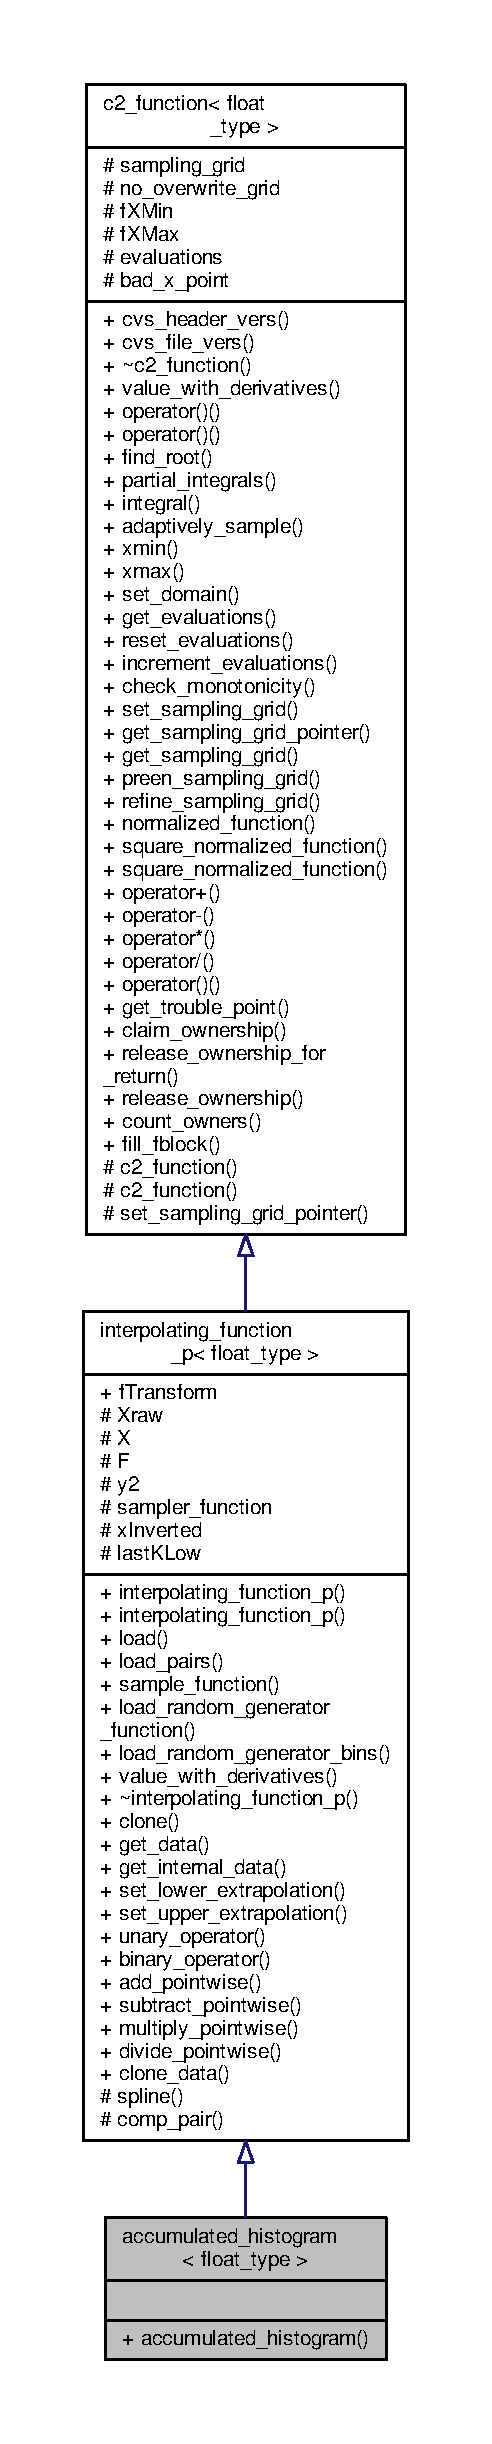
\includegraphics[height=550pt]{classaccumulated__histogram__inherit__graph}
\end{center}
\end{figure}


Collaboration diagram for accumulated\+\_\+histogram$<$ float\+\_\+type $>$\+:
\nopagebreak
\begin{figure}[H]
\begin{center}
\leavevmode
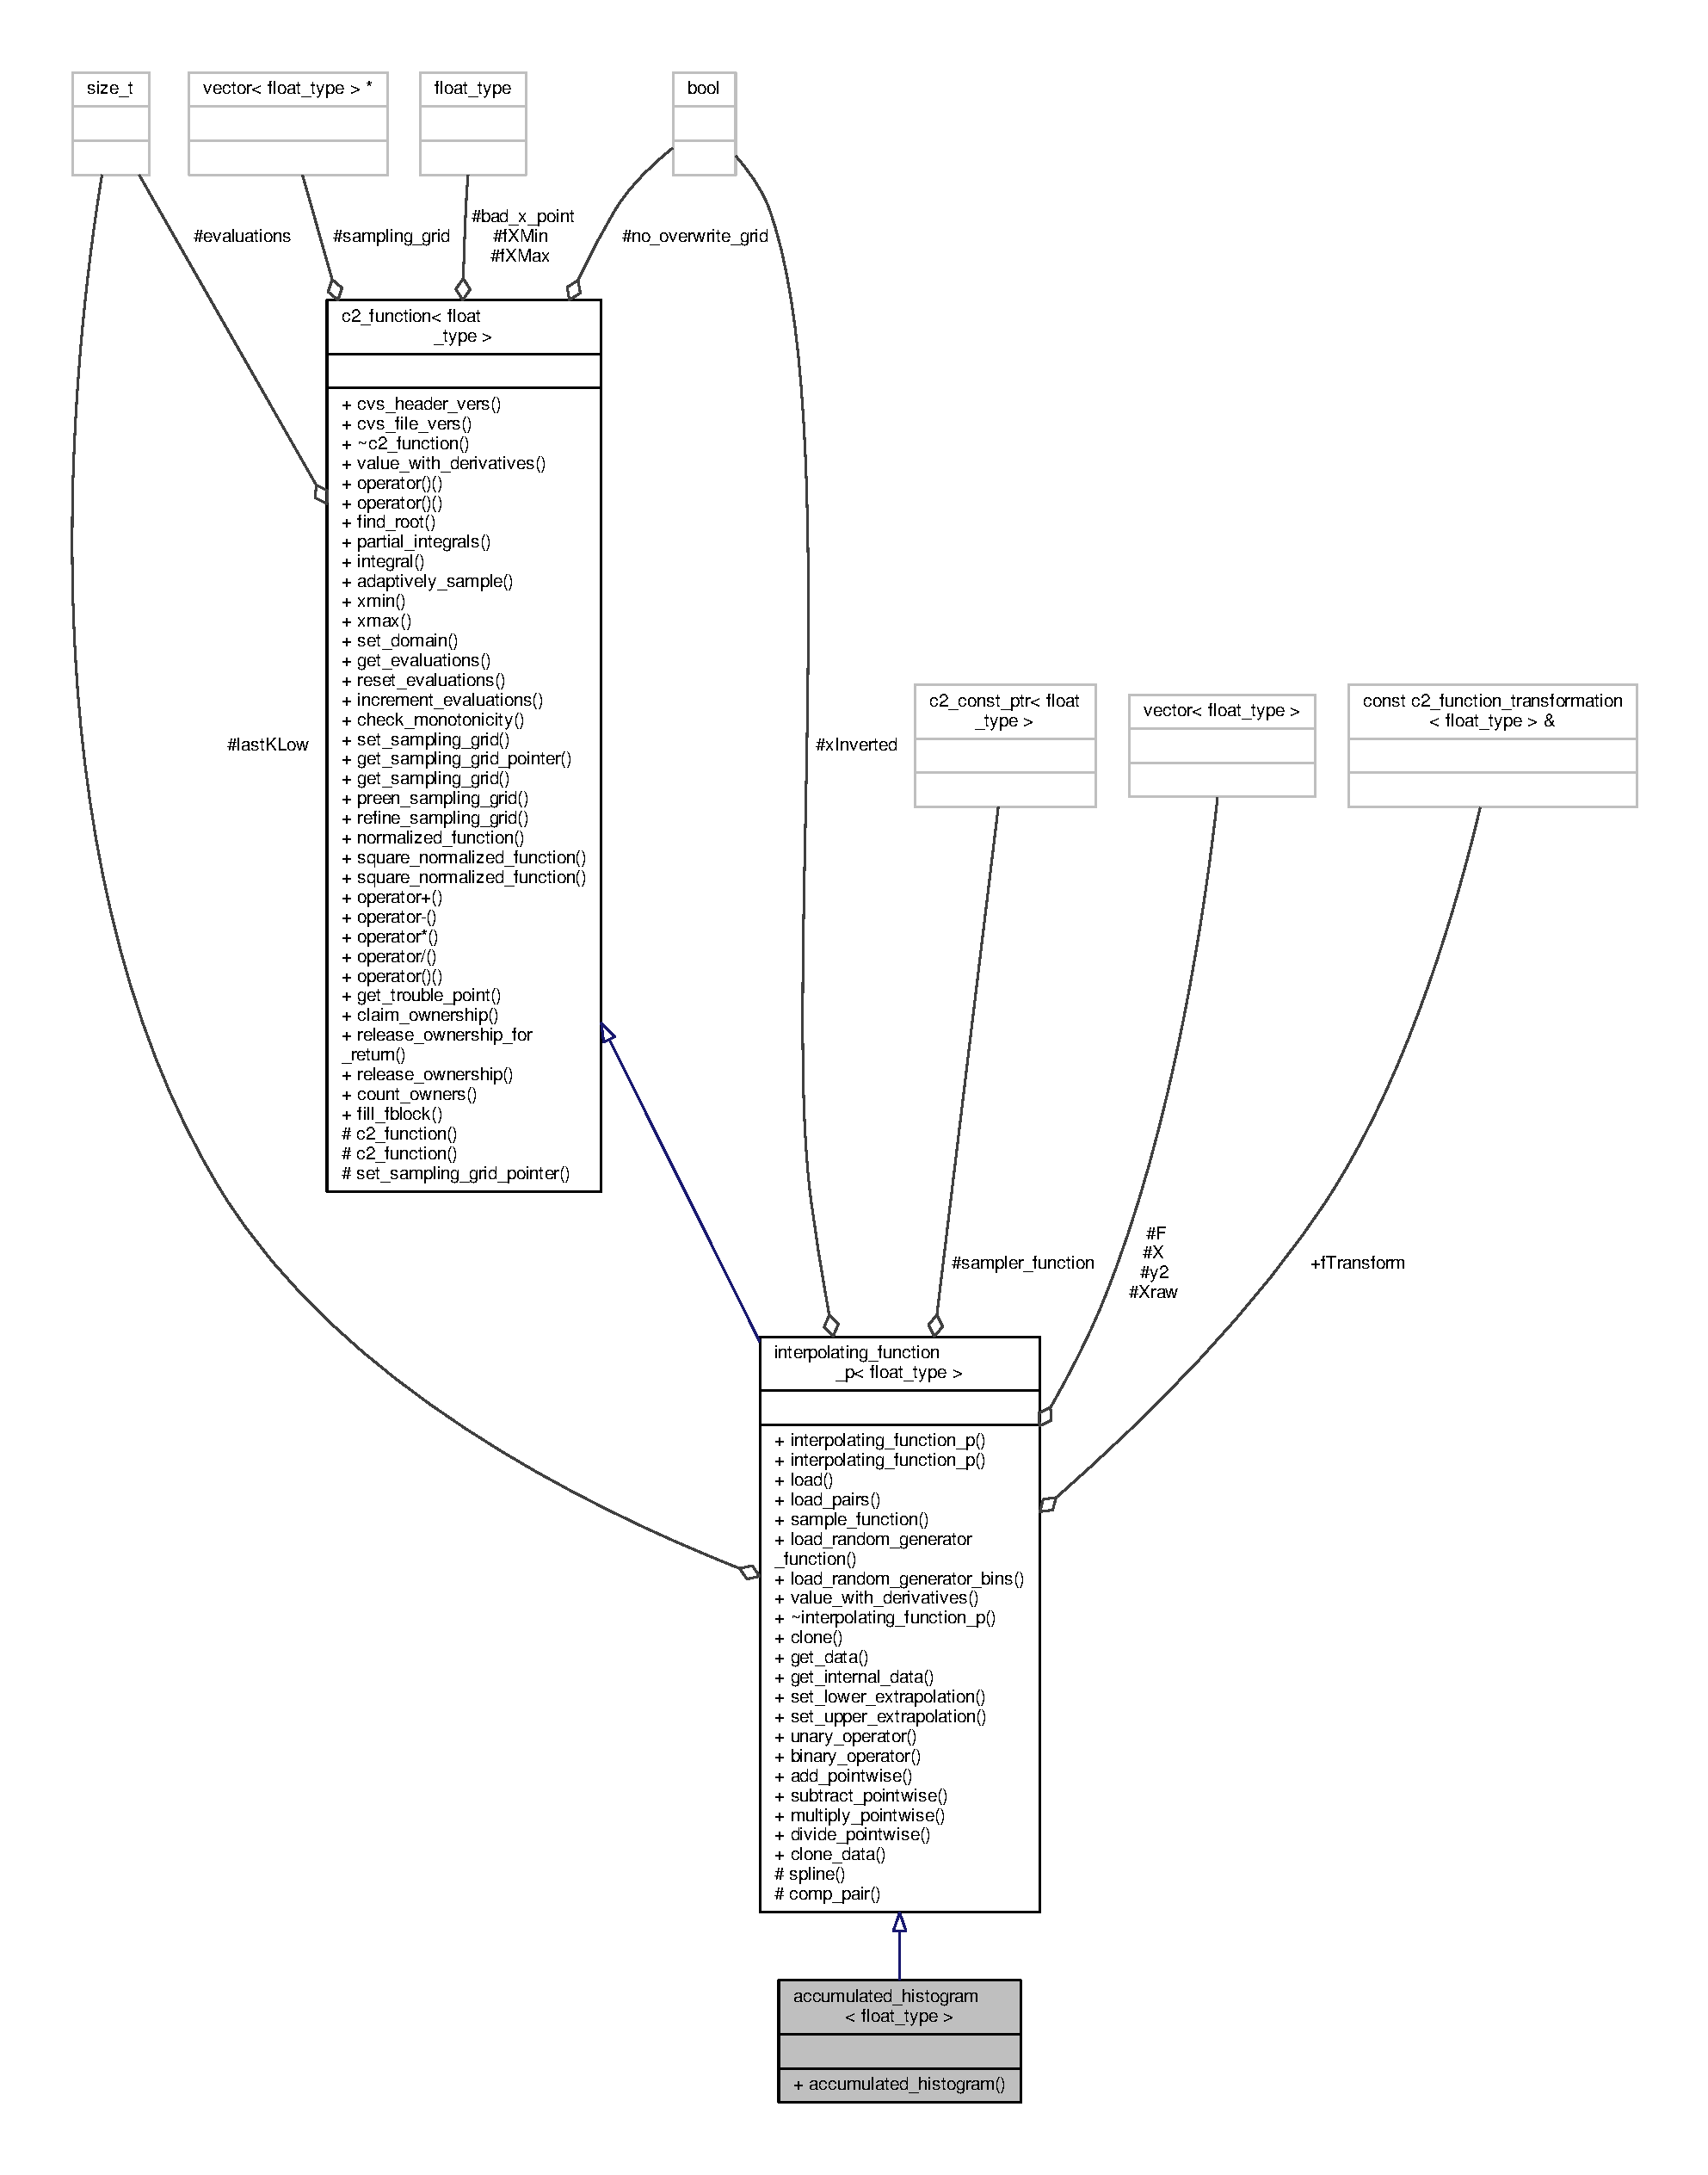
\includegraphics[width=350pt]{classaccumulated__histogram__coll__graph}
\end{center}
\end{figure}
\subsection*{Public Member Functions}
\begin{DoxyCompactItemize}
\item 
\hyperlink{classaccumulated__histogram_a54f0bb356a90baa58ff635ef8094dfc8}{accumulated\+\_\+histogram} (const std\+::vector$<$ float\+\_\+type $>$binedges, const std\+::vector$<$ float\+\_\+type $>$ binheights, bool normalize=false, bool inverse\+\_\+function=false, bool drop\+\_\+zeros=true)
\begin{DoxyCompactList}\small\item\em Construct the integrated histogram. \end{DoxyCompactList}\end{DoxyCompactItemize}
\subsection*{Additional Inherited Members}


\subsection{Detailed Description}
\subsubsection*{template$<$typename float\+\_\+type = double$>$\\*
class accumulated\+\_\+histogram$<$ float\+\_\+type $>$}

An \hyperlink{classinterpolating__function__p}{interpolating\+\_\+function\+\_\+p} which is the cumulative integral of a histogram.

Note than binedges should be one element longer than binheights, since the lower \& upper edges are specified. Note that this is a malformed spline, since the second derivatives are all zero, so it has less continuity. Also, note that the bin edges can be given in backwards order to generate the reversed accumulation (starting at the high end) 

\subsection{Constructor \& Destructor Documentation}
\index{accumulated\+\_\+histogram@{accumulated\+\_\+histogram}!accumulated\+\_\+histogram@{accumulated\+\_\+histogram}}
\index{accumulated\+\_\+histogram@{accumulated\+\_\+histogram}!accumulated\+\_\+histogram@{accumulated\+\_\+histogram}}
\subsubsection[{\texorpdfstring{accumulated\+\_\+histogram(const std\+::vector$<$ float\+\_\+type $>$binedges, const std\+::vector$<$ float\+\_\+type $>$ binheights, bool normalize=false, bool inverse\+\_\+function=false, bool drop\+\_\+zeros=true)}{accumulated_histogram(const std::vector< float_type >binedges, const std::vector< float_type > binheights, bool normalize=false, bool inverse_function=false, bool drop_zeros=true)}}]{\setlength{\rightskip}{0pt plus 5cm}template$<$typename float\+\_\+type  = double$>$ {\bf accumulated\+\_\+histogram}$<$ float\+\_\+type $>$\+::{\bf accumulated\+\_\+histogram} (
\begin{DoxyParamCaption}
\item[{const std\+::vector$<$ float\+\_\+type $>$}]{binedges, }
\item[{const std\+::vector$<$ float\+\_\+type $>$}]{binheights, }
\item[{bool}]{normalize = {\ttfamily false}, }
\item[{bool}]{inverse\+\_\+function = {\ttfamily false}, }
\item[{bool}]{drop\+\_\+zeros = {\ttfamily true}}
\end{DoxyParamCaption}
)}\hypertarget{classaccumulated__histogram_a54f0bb356a90baa58ff635ef8094dfc8}{}\label{classaccumulated__histogram_a54f0bb356a90baa58ff635ef8094dfc8}


Construct the integrated histogram. 


\begin{DoxyParams}{Parameters}
{\em binedges} & the edges of the bins in {\itshape binheights}. It should have one more element than {\itshape binheights} \\
\hline
{\em binheights} & the number of counts in each bin. \\
\hline
{\em normalize} & if true, normalize integral to 1 \\
\hline
{\em inverse\+\_\+function} & if true, drop zero channels, and return inverse function for random generation \\
\hline
{\em drop\+\_\+zeros} & eliminate null bins before integrating, so integral is strictly monotonic. \\
\hline
\end{DoxyParams}


The documentation for this class was generated from the following file\+:\begin{DoxyCompactItemize}
\item 
\hyperlink{c2__function_8hh}{c2\+\_\+function.\+hh}\end{DoxyCompactItemize}

\hypertarget{classarrhenius__interpolating__function__p}{}\section{arrhenius\+\_\+interpolating\+\_\+function\+\_\+p$<$ float\+\_\+type $>$ Class Template Reference}
\label{classarrhenius__interpolating__function__p}\index{arrhenius\+\_\+interpolating\+\_\+function\+\_\+p$<$ float\+\_\+type $>$@{arrhenius\+\_\+interpolating\+\_\+function\+\_\+p$<$ float\+\_\+type $>$}}


A spline with X in reciprocal space and Y transformed in log space.

Most useful for thermodynamic types of data where Y is roughly A$\ast$exp(-\/\+B/x). Typical examples are reaction rate data, and thermistor calibration data.  




{\ttfamily \#include \char`\"{}c2\+\_\+function.\+hh\char`\"{}}



Inheritance diagram for arrhenius\+\_\+interpolating\+\_\+function\+\_\+p$<$ float\+\_\+type $>$\+:
\nopagebreak
\begin{figure}[H]
\begin{center}
\leavevmode
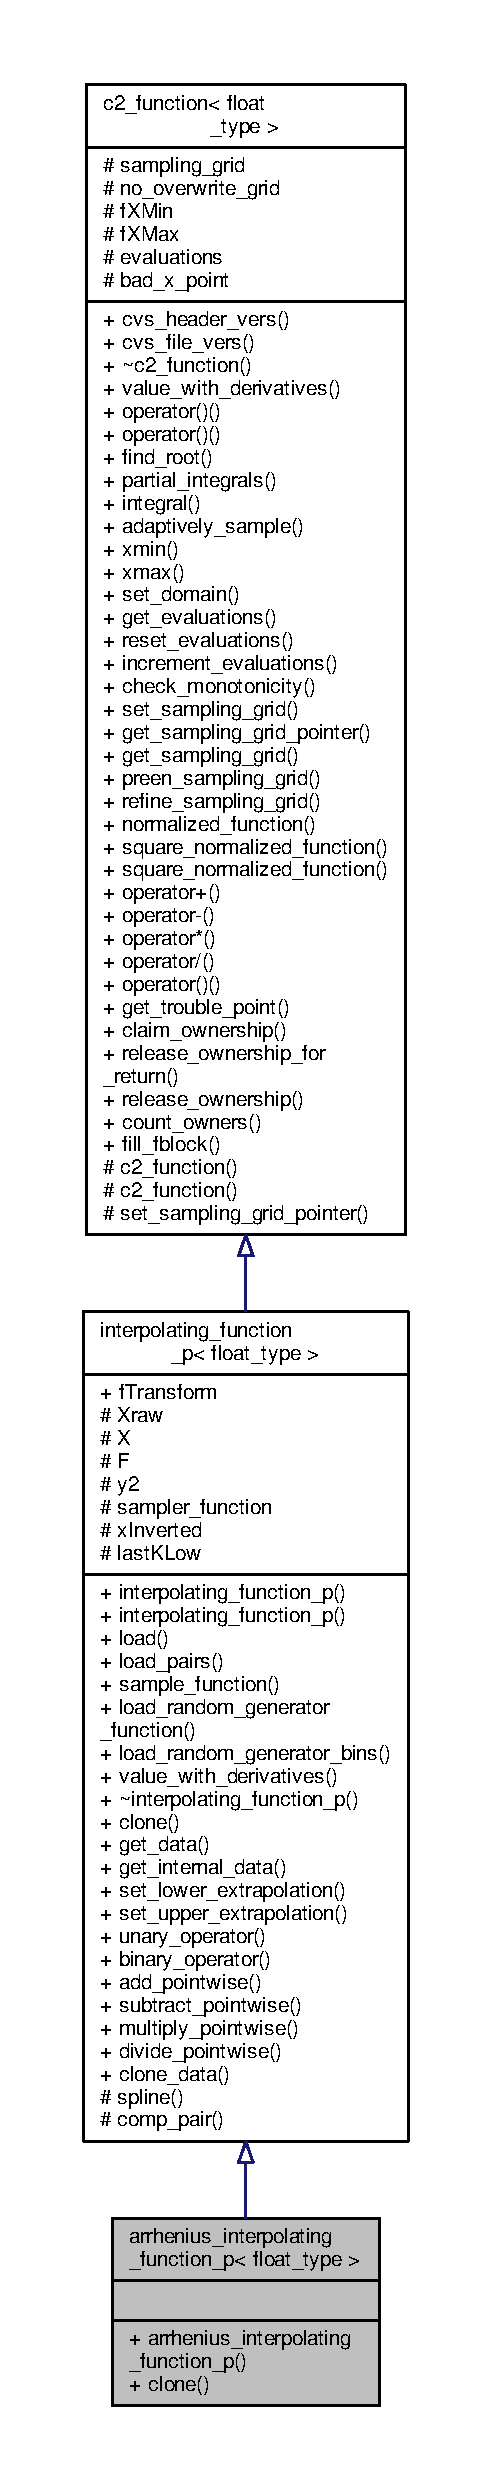
\includegraphics[height=550pt]{classarrhenius__interpolating__function__p__inherit__graph}
\end{center}
\end{figure}


Collaboration diagram for arrhenius\+\_\+interpolating\+\_\+function\+\_\+p$<$ float\+\_\+type $>$\+:
\nopagebreak
\begin{figure}[H]
\begin{center}
\leavevmode
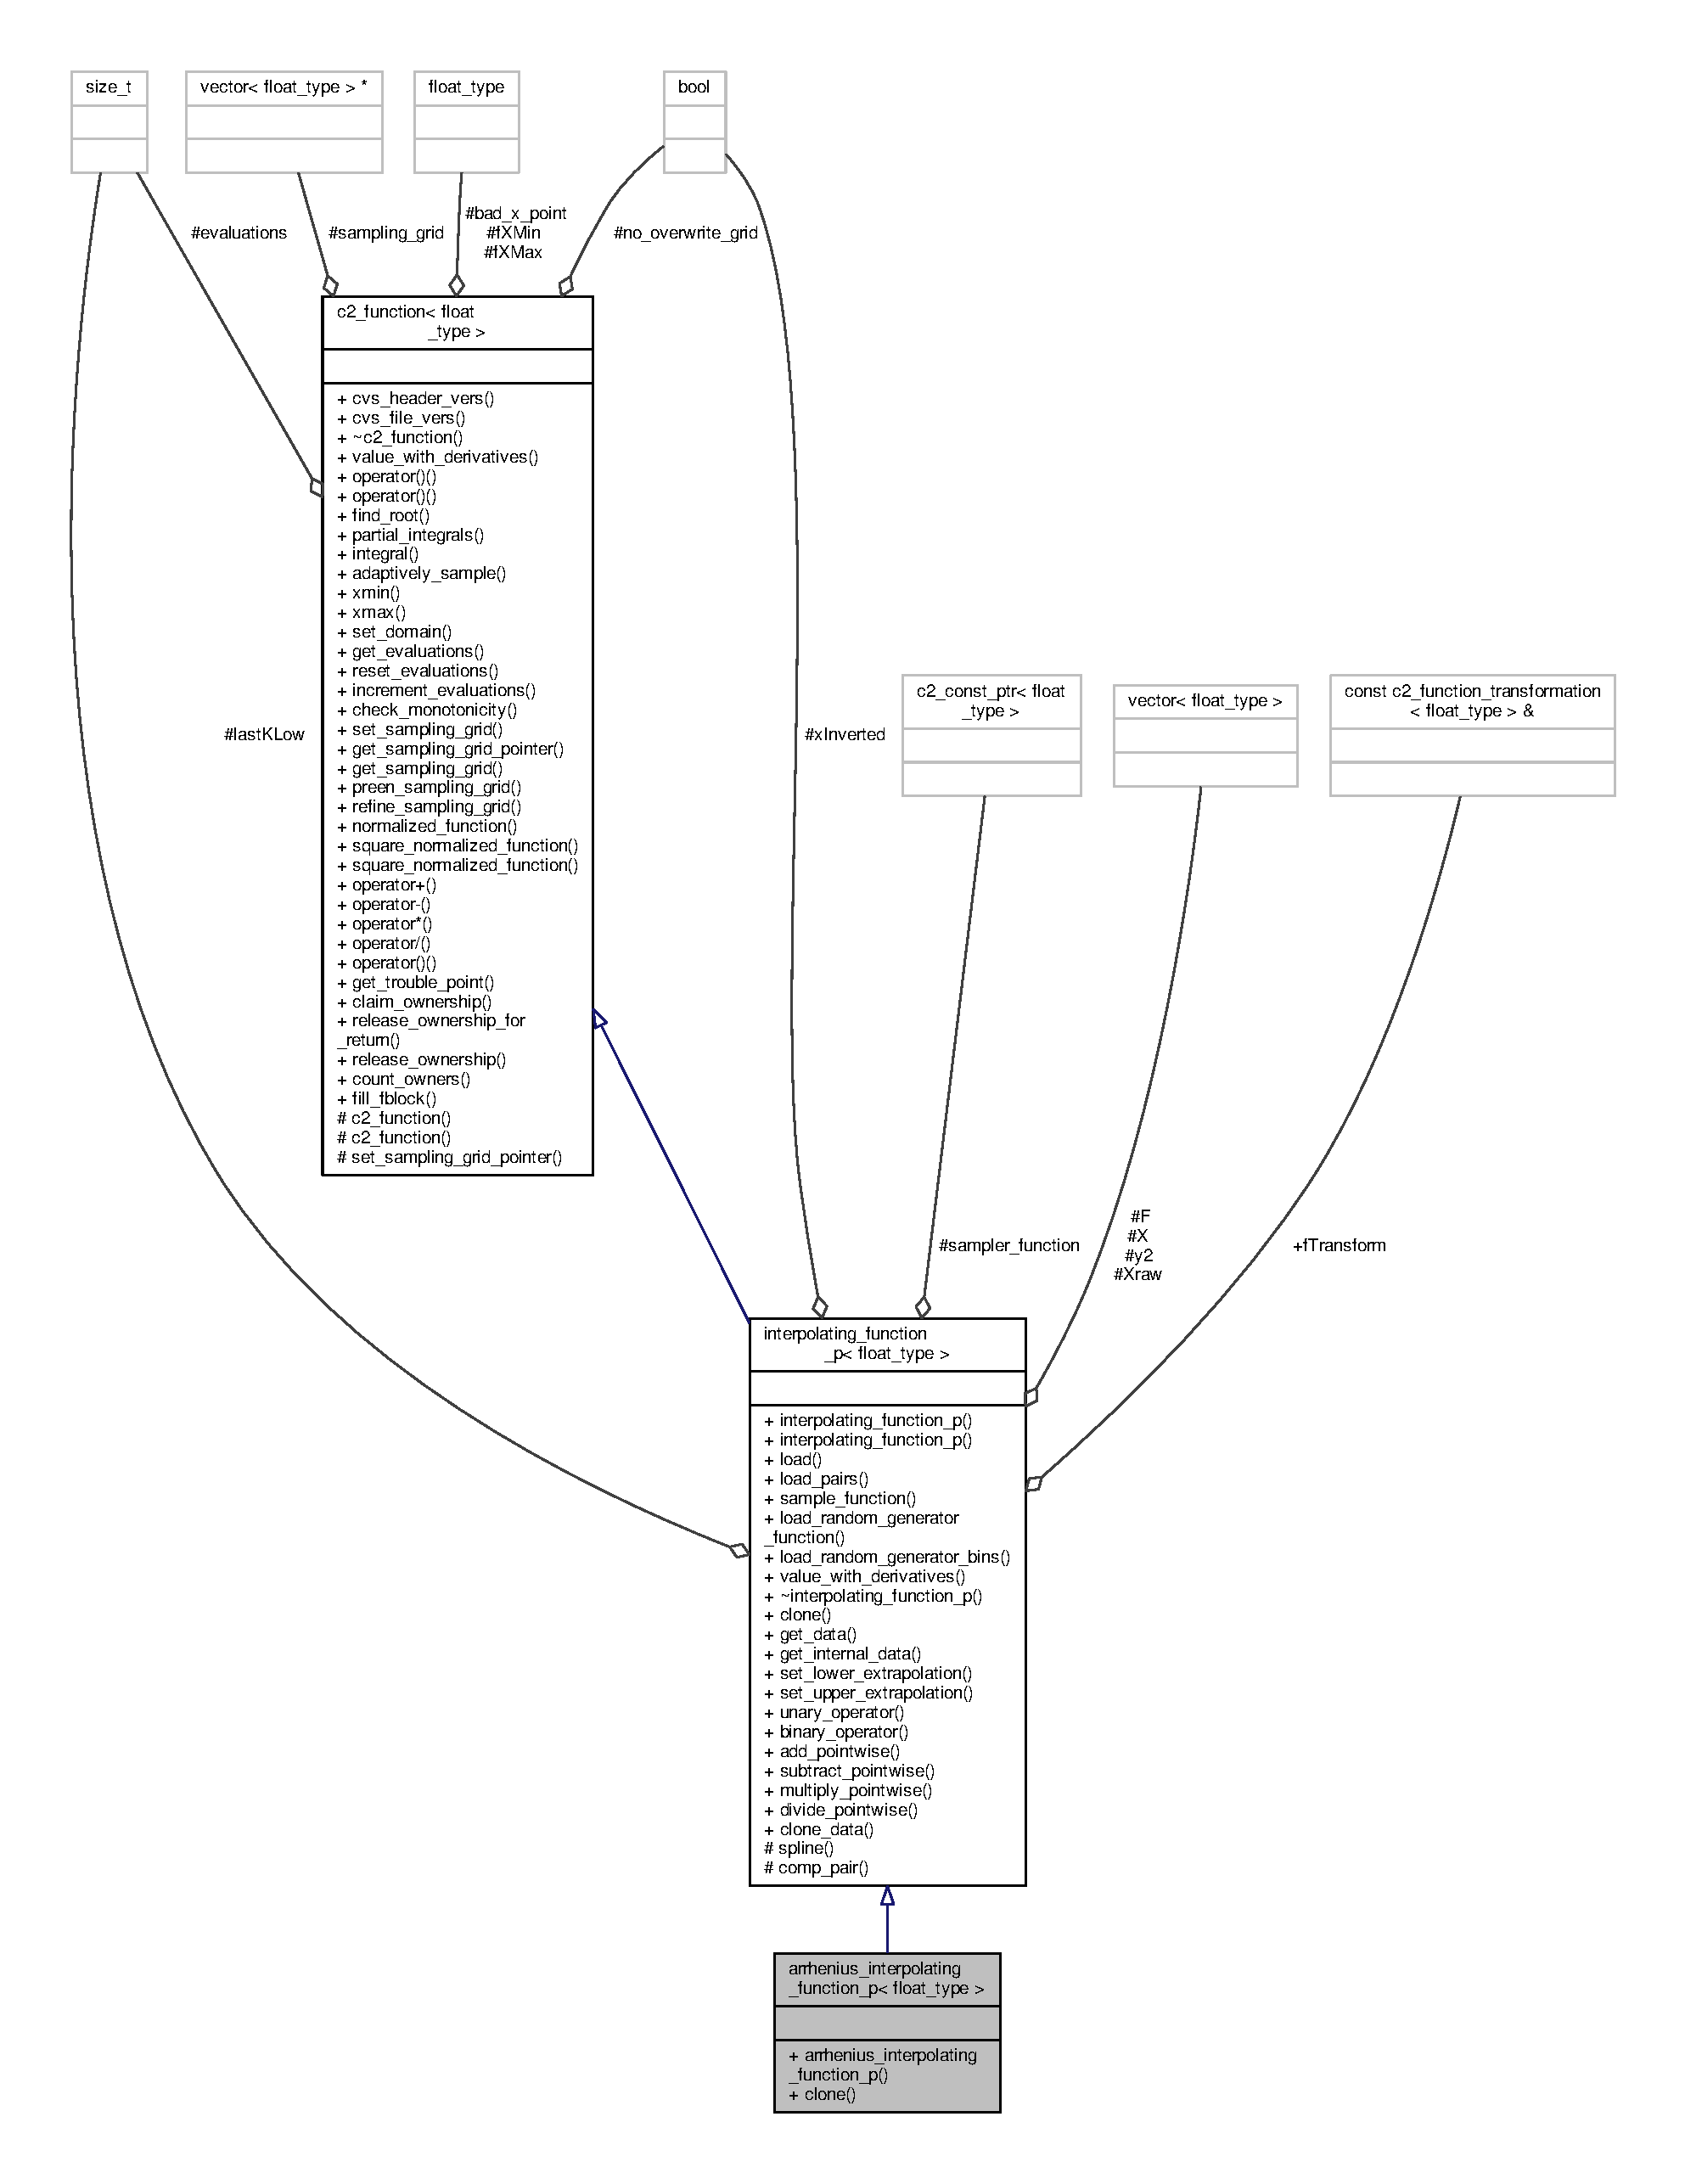
\includegraphics[width=350pt]{classarrhenius__interpolating__function__p__coll__graph}
\end{center}
\end{figure}
\subsection*{Public Member Functions}
\begin{DoxyCompactItemize}
\item 
\hyperlink{classarrhenius__interpolating__function__p_ad0557b1774e14d7a310aa14bb64d6bc5}{arrhenius\+\_\+interpolating\+\_\+function\+\_\+p} ()
\begin{DoxyCompactList}\small\item\em an empty arrhenius cubic-\/spline \hyperlink{classinterpolating__function__p}{interpolating\+\_\+function\+\_\+p} \end{DoxyCompactList}\item 
virtual \hyperlink{classinterpolating__function__p}{interpolating\+\_\+function\+\_\+p}$<$ float\+\_\+type $>$ \& \hyperlink{classarrhenius__interpolating__function__p_aad3096d6df4488e4226036fb52298ffa}{clone} () const   throw (c2\+\_\+exception)
\begin{DoxyCompactList}\small\item\em create a new, empty interpolating function of this type (virtual constructor) \end{DoxyCompactList}\end{DoxyCompactItemize}
\subsection*{Additional Inherited Members}


\subsection{Detailed Description}
\subsubsection*{template$<$typename float\+\_\+type = double$>$\\*
class arrhenius\+\_\+interpolating\+\_\+function\+\_\+p$<$ float\+\_\+type $>$}

A spline with X in reciprocal space and Y transformed in log space.

Most useful for thermodynamic types of data where Y is roughly A$\ast$exp(-\/\+B/x). Typical examples are reaction rate data, and thermistor calibration data. 

The factory function \hyperlink{classc2__factory_ac2ab3145f84167194ba1ff71aaaa6ffe}{c2\+\_\+factory\+::arrhenius\+\_\+interpolating\+\_\+function()} creates $\ast$new \hyperlink{classarrhenius__interpolating__function__p_ad0557b1774e14d7a310aa14bb64d6bc5}{arrhenius\+\_\+interpolating\+\_\+function\+\_\+p()} 

\subsection{Constructor \& Destructor Documentation}
\index{arrhenius\+\_\+interpolating\+\_\+function\+\_\+p@{arrhenius\+\_\+interpolating\+\_\+function\+\_\+p}!arrhenius\+\_\+interpolating\+\_\+function\+\_\+p@{arrhenius\+\_\+interpolating\+\_\+function\+\_\+p}}
\index{arrhenius\+\_\+interpolating\+\_\+function\+\_\+p@{arrhenius\+\_\+interpolating\+\_\+function\+\_\+p}!arrhenius\+\_\+interpolating\+\_\+function\+\_\+p@{arrhenius\+\_\+interpolating\+\_\+function\+\_\+p}}
\subsubsection[{\texorpdfstring{arrhenius\+\_\+interpolating\+\_\+function\+\_\+p()}{arrhenius_interpolating_function_p()}}]{\setlength{\rightskip}{0pt plus 5cm}template$<$typename float\+\_\+type  = double$>$ {\bf arrhenius\+\_\+interpolating\+\_\+function\+\_\+p}$<$ float\+\_\+type $>$\+::{\bf arrhenius\+\_\+interpolating\+\_\+function\+\_\+p} (
\begin{DoxyParamCaption}
{}
\end{DoxyParamCaption}
)\hspace{0.3cm}{\ttfamily [inline]}}\hypertarget{classarrhenius__interpolating__function__p_ad0557b1774e14d7a310aa14bb64d6bc5}{}\label{classarrhenius__interpolating__function__p_ad0557b1774e14d7a310aa14bb64d6bc5}


an empty arrhenius cubic-\/spline \hyperlink{classinterpolating__function__p}{interpolating\+\_\+function\+\_\+p} 



\subsection{Member Function Documentation}
\index{arrhenius\+\_\+interpolating\+\_\+function\+\_\+p@{arrhenius\+\_\+interpolating\+\_\+function\+\_\+p}!clone@{clone}}
\index{clone@{clone}!arrhenius\+\_\+interpolating\+\_\+function\+\_\+p@{arrhenius\+\_\+interpolating\+\_\+function\+\_\+p}}
\subsubsection[{\texorpdfstring{clone() const }{clone() const }}]{\setlength{\rightskip}{0pt plus 5cm}template$<$typename float\+\_\+type  = double$>$ virtual {\bf interpolating\+\_\+function\+\_\+p}$<$float\+\_\+type$>$\& {\bf arrhenius\+\_\+interpolating\+\_\+function\+\_\+p}$<$ float\+\_\+type $>$\+::clone (
\begin{DoxyParamCaption}
{}
\end{DoxyParamCaption}
) const throw  {\bf c2\+\_\+exception}) \hspace{0.3cm}{\ttfamily [inline]}, {\ttfamily [virtual]}}\hypertarget{classarrhenius__interpolating__function__p_aad3096d6df4488e4226036fb52298ffa}{}\label{classarrhenius__interpolating__function__p_aad3096d6df4488e4226036fb52298ffa}


create a new, empty interpolating function of this type (virtual constructor) 



Reimplemented from \hyperlink{classinterpolating__function__p_a8a2c601fde0ef3226e51d1f51b4f5f2f}{interpolating\+\_\+function\+\_\+p$<$ float\+\_\+type $>$}.



The documentation for this class was generated from the following file\+:\begin{DoxyCompactItemize}
\item 
\hyperlink{c2__function_8hh}{c2\+\_\+function.\+hh}\end{DoxyCompactItemize}

\hypertarget{classBGField1}{}\section{B\+G\+Field1 Class Reference}
\label{classBGField1}\index{B\+G\+Field1@{B\+G\+Field1}}


{\ttfamily \#include \char`\"{}B\+G\+Field1.\+hh\char`\"{}}



Inheritance diagram for B\+G\+Field1\+:
\nopagebreak
\begin{figure}[H]
\begin{center}
\leavevmode
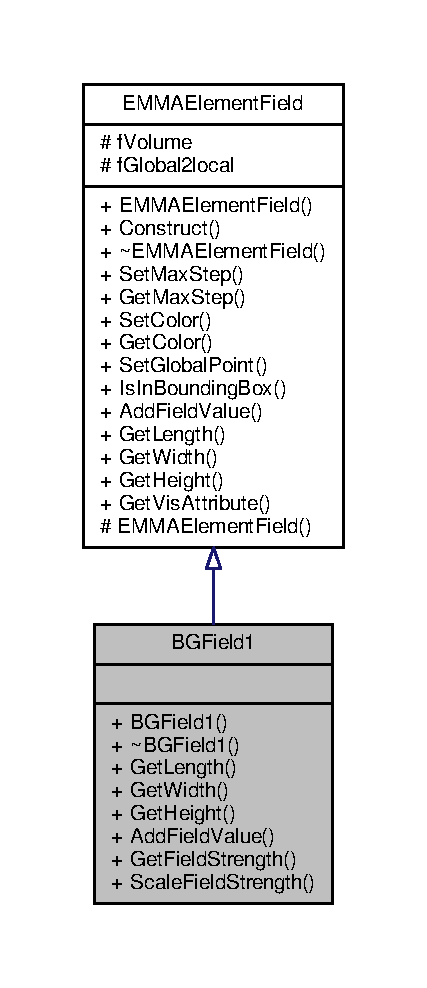
\includegraphics[width=205pt]{classBGField1__inherit__graph}
\end{center}
\end{figure}


Collaboration diagram for B\+G\+Field1\+:
\nopagebreak
\begin{figure}[H]
\begin{center}
\leavevmode
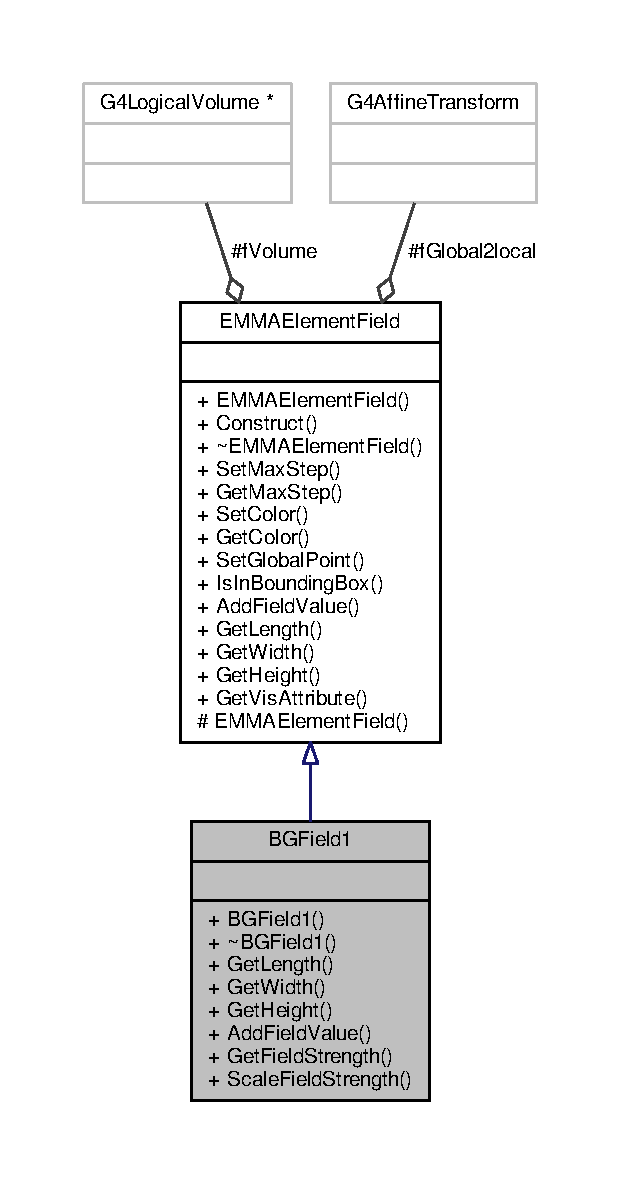
\includegraphics[height=550pt]{classBGField1__coll__graph}
\end{center}
\end{figure}
\subsection*{Public Member Functions}
\begin{DoxyCompactItemize}
\item 
\hyperlink{classBGField1_a1bc9224e371e4e289fb1104303a5e336}{B\+G\+Field1} (G4double xoffset, G4double zoffset, G4double zbefore, G4double zafter, G4\+Logical\+Volume $\ast$, G4\+Three\+Vector)
\item 
\hyperlink{classBGField1_a9f32073e612f55662a302942f5015177}{$\sim$\+B\+G\+Field1} ()
\item 
virtual G4double \hyperlink{classBGField1_a11ba0cbb1190e5f2340aa7907f7d66f9}{Get\+Length} ()
\item 
virtual G4double \hyperlink{classBGField1_a44eca4d023aac7e4bf9dd959760afa28}{Get\+Width} ()
\item 
virtual G4double \hyperlink{classBGField1_af1b93a1566b1a53a00eb1d3ccc77815a}{Get\+Height} ()
\item 
virtual void \hyperlink{classBGField1_aa6119f980c4bb2eb52067c1e66ffbae4}{Add\+Field\+Value} (const G4double Point\mbox{[}3\mbox{]}, G4double field\mbox{[}6\mbox{]}) const 
\item 
G4double \hyperlink{classBGField1_a105ef833b5e57d8624536ba7fcf4e382}{Get\+Field\+Strength} ()
\item 
void \hyperlink{classBGField1_ab0123f55a83d4a8a4c17b401478759a0}{Scale\+Field\+Strength} (G4double msf)
\end{DoxyCompactItemize}
\subsection*{Additional Inherited Members}


\subsection{Constructor \& Destructor Documentation}
\index{B\+G\+Field1@{B\+G\+Field1}!B\+G\+Field1@{B\+G\+Field1}}
\index{B\+G\+Field1@{B\+G\+Field1}!B\+G\+Field1@{B\+G\+Field1}}
\subsubsection[{\texorpdfstring{B\+G\+Field1(\+G4double xoffset, G4double zoffset, G4double zbefore, G4double zafter, G4\+Logical\+Volume $\ast$, G4\+Three\+Vector)}{BGField1(G4double xoffset, G4double zoffset, G4double zbefore, G4double zafter, G4LogicalVolume *, G4ThreeVector)}}]{\setlength{\rightskip}{0pt plus 5cm}B\+G\+Field1\+::\+B\+G\+Field1 (
\begin{DoxyParamCaption}
\item[{G4double}]{xoffset, }
\item[{G4double}]{zoffset, }
\item[{G4double}]{zbefore, }
\item[{G4double}]{zafter, }
\item[{G4\+Logical\+Volume $\ast$}]{, }
\item[{G4\+Three\+Vector}]{}
\end{DoxyParamCaption}
)}\hypertarget{classBGField1_a1bc9224e371e4e289fb1104303a5e336}{}\label{classBGField1_a1bc9224e371e4e289fb1104303a5e336}
\index{B\+G\+Field1@{B\+G\+Field1}!````~B\+G\+Field1@{$\sim$\+B\+G\+Field1}}
\index{````~B\+G\+Field1@{$\sim$\+B\+G\+Field1}!B\+G\+Field1@{B\+G\+Field1}}
\subsubsection[{\texorpdfstring{$\sim$\+B\+G\+Field1()}{~BGField1()}}]{\setlength{\rightskip}{0pt plus 5cm}B\+G\+Field1\+::$\sim$\+B\+G\+Field1 (
\begin{DoxyParamCaption}
{}
\end{DoxyParamCaption}
)}\hypertarget{classBGField1_a9f32073e612f55662a302942f5015177}{}\label{classBGField1_a9f32073e612f55662a302942f5015177}


\subsection{Member Function Documentation}
\index{B\+G\+Field1@{B\+G\+Field1}!Add\+Field\+Value@{Add\+Field\+Value}}
\index{Add\+Field\+Value@{Add\+Field\+Value}!B\+G\+Field1@{B\+G\+Field1}}
\subsubsection[{\texorpdfstring{Add\+Field\+Value(const G4double Point[3], G4double field[6]) const }{AddFieldValue(const G4double Point[3], G4double field[6]) const }}]{\setlength{\rightskip}{0pt plus 5cm}virtual void B\+G\+Field1\+::\+Add\+Field\+Value (
\begin{DoxyParamCaption}
\item[{const G4double}]{Point\mbox{[}3\mbox{]}, }
\item[{G4double}]{field\mbox{[}6\mbox{]}}
\end{DoxyParamCaption}
) const\hspace{0.3cm}{\ttfamily [virtual]}}\hypertarget{classBGField1_aa6119f980c4bb2eb52067c1e66ffbae4}{}\label{classBGField1_aa6119f980c4bb2eb52067c1e66ffbae4}
\index{B\+G\+Field1@{B\+G\+Field1}!Get\+Field\+Strength@{Get\+Field\+Strength}}
\index{Get\+Field\+Strength@{Get\+Field\+Strength}!B\+G\+Field1@{B\+G\+Field1}}
\subsubsection[{\texorpdfstring{Get\+Field\+Strength()}{GetFieldStrength()}}]{\setlength{\rightskip}{0pt plus 5cm}G4double B\+G\+Field1\+::\+Get\+Field\+Strength (
\begin{DoxyParamCaption}
{}
\end{DoxyParamCaption}
)\hspace{0.3cm}{\ttfamily [inline]}}\hypertarget{classBGField1_a105ef833b5e57d8624536ba7fcf4e382}{}\label{classBGField1_a105ef833b5e57d8624536ba7fcf4e382}
\index{B\+G\+Field1@{B\+G\+Field1}!Get\+Height@{Get\+Height}}
\index{Get\+Height@{Get\+Height}!B\+G\+Field1@{B\+G\+Field1}}
\subsubsection[{\texorpdfstring{Get\+Height()}{GetHeight()}}]{\setlength{\rightskip}{0pt plus 5cm}virtual G4double B\+G\+Field1\+::\+Get\+Height (
\begin{DoxyParamCaption}
{}
\end{DoxyParamCaption}
)\hspace{0.3cm}{\ttfamily [inline]}, {\ttfamily [virtual]}}\hypertarget{classBGField1_af1b93a1566b1a53a00eb1d3ccc77815a}{}\label{classBGField1_af1b93a1566b1a53a00eb1d3ccc77815a}


Implements \hyperlink{classEMMAElementField_a3cbd223805ba24b5313e16ca540c326c}{E\+M\+M\+A\+Element\+Field}.

\index{B\+G\+Field1@{B\+G\+Field1}!Get\+Length@{Get\+Length}}
\index{Get\+Length@{Get\+Length}!B\+G\+Field1@{B\+G\+Field1}}
\subsubsection[{\texorpdfstring{Get\+Length()}{GetLength()}}]{\setlength{\rightskip}{0pt plus 5cm}virtual G4double B\+G\+Field1\+::\+Get\+Length (
\begin{DoxyParamCaption}
{}
\end{DoxyParamCaption}
)\hspace{0.3cm}{\ttfamily [inline]}, {\ttfamily [virtual]}}\hypertarget{classBGField1_a11ba0cbb1190e5f2340aa7907f7d66f9}{}\label{classBGField1_a11ba0cbb1190e5f2340aa7907f7d66f9}


Implements \hyperlink{classEMMAElementField_adb2d90c3fdf25e17be541903bffca35b}{E\+M\+M\+A\+Element\+Field}.

\index{B\+G\+Field1@{B\+G\+Field1}!Get\+Width@{Get\+Width}}
\index{Get\+Width@{Get\+Width}!B\+G\+Field1@{B\+G\+Field1}}
\subsubsection[{\texorpdfstring{Get\+Width()}{GetWidth()}}]{\setlength{\rightskip}{0pt plus 5cm}virtual G4double B\+G\+Field1\+::\+Get\+Width (
\begin{DoxyParamCaption}
{}
\end{DoxyParamCaption}
)\hspace{0.3cm}{\ttfamily [inline]}, {\ttfamily [virtual]}}\hypertarget{classBGField1_a44eca4d023aac7e4bf9dd959760afa28}{}\label{classBGField1_a44eca4d023aac7e4bf9dd959760afa28}


Implements \hyperlink{classEMMAElementField_a41708a8f1e72d7788c0a53c80c297bf9}{E\+M\+M\+A\+Element\+Field}.

\index{B\+G\+Field1@{B\+G\+Field1}!Scale\+Field\+Strength@{Scale\+Field\+Strength}}
\index{Scale\+Field\+Strength@{Scale\+Field\+Strength}!B\+G\+Field1@{B\+G\+Field1}}
\subsubsection[{\texorpdfstring{Scale\+Field\+Strength(\+G4double msf)}{ScaleFieldStrength(G4double msf)}}]{\setlength{\rightskip}{0pt plus 5cm}void B\+G\+Field1\+::\+Scale\+Field\+Strength (
\begin{DoxyParamCaption}
\item[{G4double}]{msf}
\end{DoxyParamCaption}
)\hspace{0.3cm}{\ttfamily [inline]}}\hypertarget{classBGField1_ab0123f55a83d4a8a4c17b401478759a0}{}\label{classBGField1_ab0123f55a83d4a8a4c17b401478759a0}


The documentation for this class was generated from the following file\+:\begin{DoxyCompactItemize}
\item 
\hyperlink{BGField1_8hh}{B\+G\+Field1.\+hh}\end{DoxyCompactItemize}

\hypertarget{classBGField2}{\section{B\-G\-Field2 Class Reference}
\label{classBGField2}\index{B\-G\-Field2@{B\-G\-Field2}}
}
Inheritance diagram for B\-G\-Field2\-:\begin{figure}[H]
\begin{center}
\leavevmode
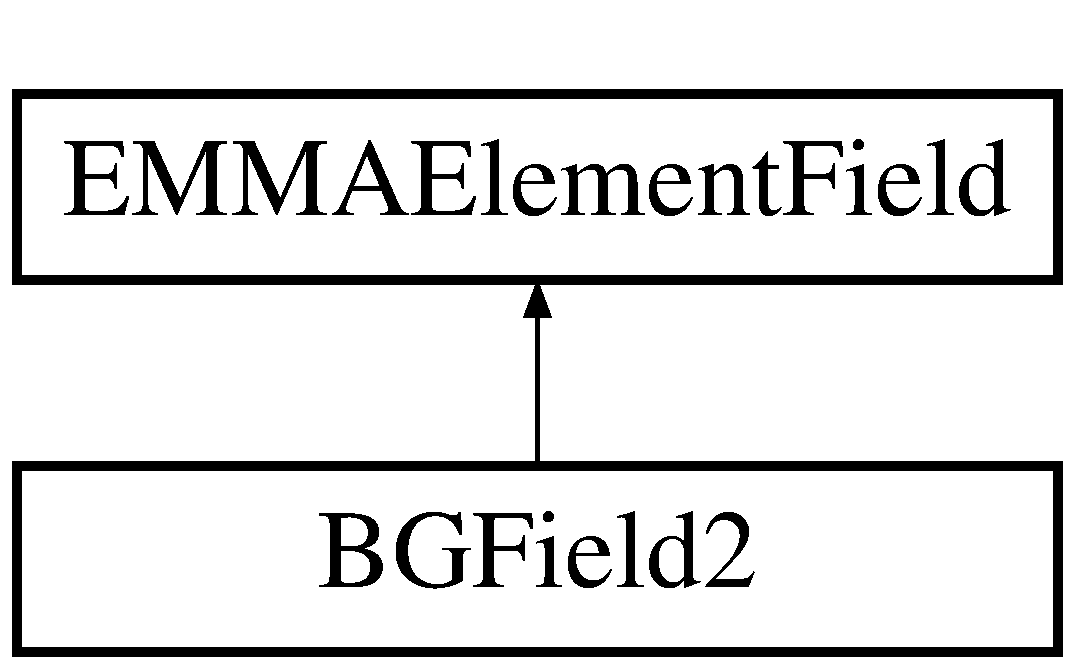
\includegraphics[height=2.000000cm]{classBGField2}
\end{center}
\end{figure}
\subsection*{Public Member Functions}
\begin{DoxyCompactItemize}
\item 
\hypertarget{classBGField2_abd68036adc384301852a843bb85bc704}{{\bfseries B\-G\-Field2} (G4double xoffset, G4double zoffset, G4double zbefore, G4double zafter, G4\-Logical\-Volume $\ast$, G4\-Three\-Vector)}\label{classBGField2_abd68036adc384301852a843bb85bc704}

\item 
\hypertarget{classBGField2_a856d0ce173b04e35c0e59ab14694d6ac}{virtual G4double {\bfseries Get\-Length} ()}\label{classBGField2_a856d0ce173b04e35c0e59ab14694d6ac}

\item 
\hypertarget{classBGField2_aa73fc7a95de254dd1aaba6d7b6248c68}{virtual G4double {\bfseries Get\-Width} ()}\label{classBGField2_aa73fc7a95de254dd1aaba6d7b6248c68}

\item 
\hypertarget{classBGField2_a8eb93f9ddd438617d363e8b194908d64}{virtual G4double {\bfseries Get\-Height} ()}\label{classBGField2_a8eb93f9ddd438617d363e8b194908d64}

\item 
\hypertarget{classBGField2_a6300d564c8722820ee8dd7d215283116}{virtual void {\bfseries Add\-Field\-Value} (const G4double Point\mbox{[}3\mbox{]}, G4double field\mbox{[}6\mbox{]}) const }\label{classBGField2_a6300d564c8722820ee8dd7d215283116}

\item 
\hypertarget{classBGField2_ac93970710ba6895256e4dba9ce459c1c}{G4double {\bfseries Get\-Field\-Strength} ()}\label{classBGField2_ac93970710ba6895256e4dba9ce459c1c}

\item 
\hypertarget{classBGField2_ae7f476b27eace05e7c6a6176e774eb77}{void {\bfseries Scale\-Field\-Strength} (G4double msf)}\label{classBGField2_ae7f476b27eace05e7c6a6176e774eb77}

\end{DoxyCompactItemize}
\subsection*{Additional Inherited Members}


The documentation for this class was generated from the following file\-:\begin{DoxyCompactItemize}
\item 
\hyperlink{BGField2_8hh}{B\-G\-Field2.\-hh}\end{DoxyCompactItemize}

\hypertarget{classBGField3}{\section{B\-G\-Field3 Class Reference}
\label{classBGField3}\index{B\-G\-Field3@{B\-G\-Field3}}
}
Inheritance diagram for B\-G\-Field3\-:\begin{figure}[H]
\begin{center}
\leavevmode
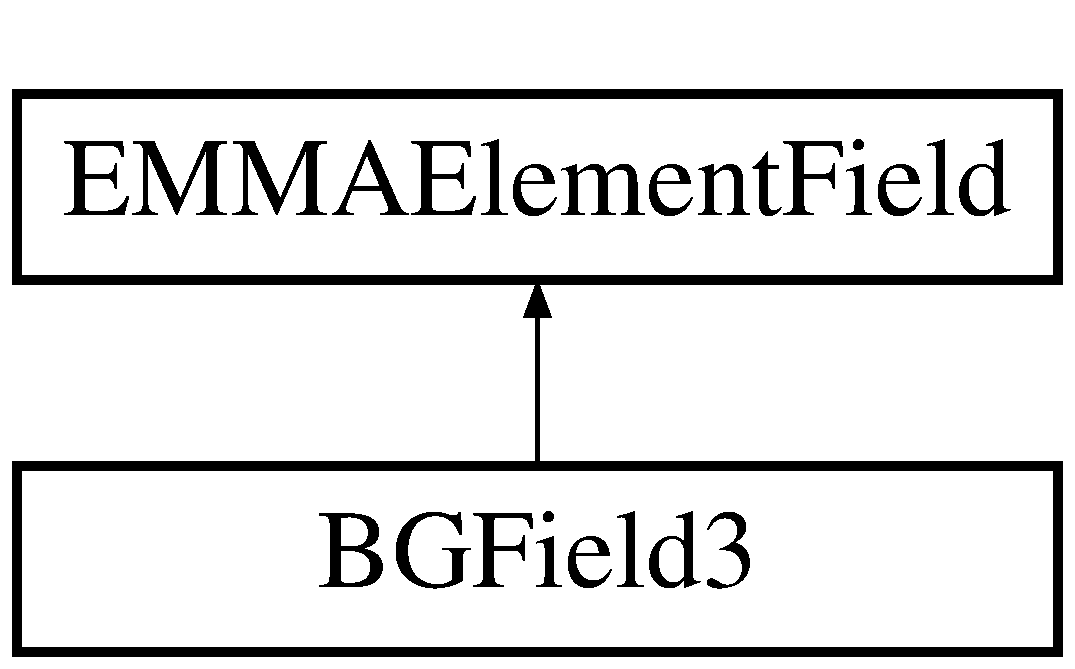
\includegraphics[height=2.000000cm]{classBGField3}
\end{center}
\end{figure}
\subsection*{Public Member Functions}
\begin{DoxyCompactItemize}
\item 
\hypertarget{classBGField3_af114b557b150290f35c94127763d7bab}{{\bfseries B\-G\-Field3} (G4double xoffset, G4double zoffset, G4double zbefore, G4double zafter, G4\-Logical\-Volume $\ast$, G4\-Three\-Vector)}\label{classBGField3_af114b557b150290f35c94127763d7bab}

\item 
\hypertarget{classBGField3_ae49dd0f301f73bae6fae3d2672823cf8}{virtual G4double {\bfseries Get\-Length} ()}\label{classBGField3_ae49dd0f301f73bae6fae3d2672823cf8}

\item 
\hypertarget{classBGField3_a84aaf81a6f511ca8d726c94d52f30336}{virtual G4double {\bfseries Get\-Width} ()}\label{classBGField3_a84aaf81a6f511ca8d726c94d52f30336}

\item 
\hypertarget{classBGField3_a9a3274bc5f550093663680da846ba954}{virtual G4double {\bfseries Get\-Height} ()}\label{classBGField3_a9a3274bc5f550093663680da846ba954}

\item 
\hypertarget{classBGField3_a994e1d640acab76909cc82abbd7a8c42}{virtual void {\bfseries Add\-Field\-Value} (const G4double Point\mbox{[}3\mbox{]}, G4double field\mbox{[}6\mbox{]}) const }\label{classBGField3_a994e1d640acab76909cc82abbd7a8c42}

\item 
\hypertarget{classBGField3_a15e84284be2eae47e39d5c793cefae77}{G4double {\bfseries Get\-Field\-Strength} ()}\label{classBGField3_a15e84284be2eae47e39d5c793cefae77}

\item 
\hypertarget{classBGField3_a5941caec9fb72a08a67d9ccd2ff6c00c}{void {\bfseries Scale\-Field\-Strength} (G4double esf)}\label{classBGField3_a5941caec9fb72a08a67d9ccd2ff6c00c}

\end{DoxyCompactItemize}
\subsection*{Additional Inherited Members}


The documentation for this class was generated from the following file\-:\begin{DoxyCompactItemize}
\item 
\hyperlink{BGField3_8hh}{B\-G\-Field3.\-hh}\end{DoxyCompactItemize}

\hypertarget{classBGField4}{}\section{B\+G\+Field4 Class Reference}
\label{classBGField4}\index{B\+G\+Field4@{B\+G\+Field4}}


{\ttfamily \#include \char`\"{}B\+G\+Field4.\+hh\char`\"{}}



Inheritance diagram for B\+G\+Field4\+:
\nopagebreak
\begin{figure}[H]
\begin{center}
\leavevmode
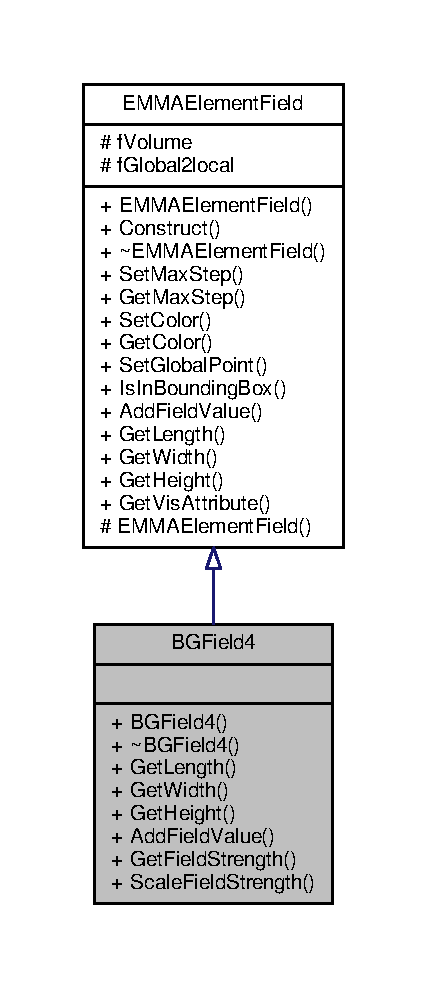
\includegraphics[width=205pt]{classBGField4__inherit__graph}
\end{center}
\end{figure}


Collaboration diagram for B\+G\+Field4\+:
\nopagebreak
\begin{figure}[H]
\begin{center}
\leavevmode
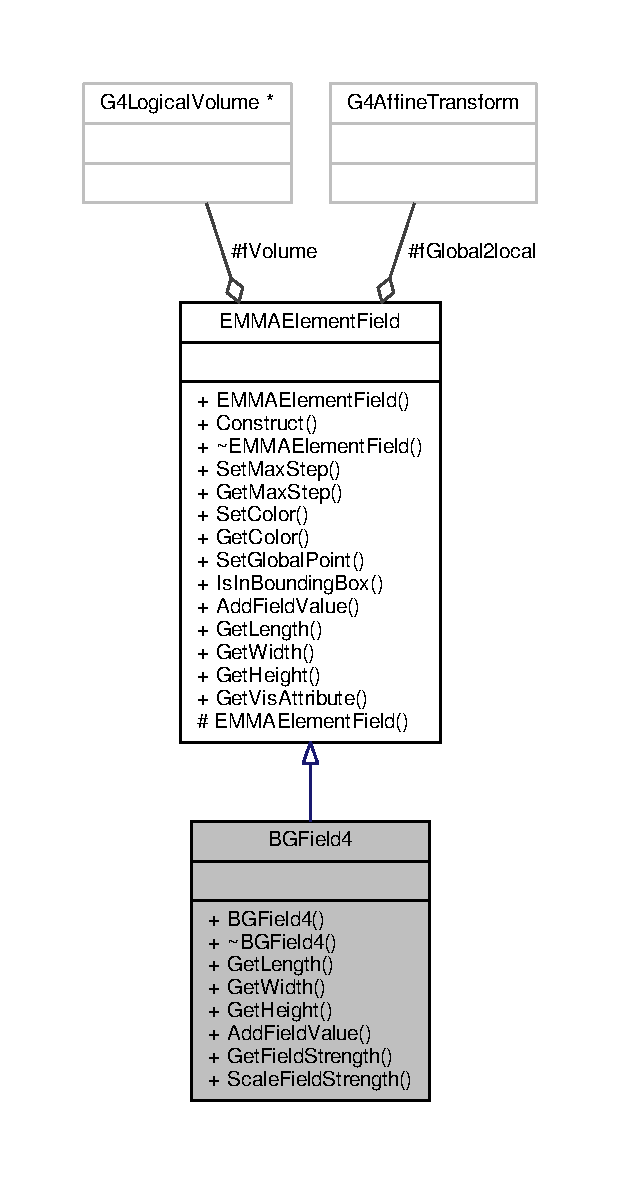
\includegraphics[height=550pt]{classBGField4__coll__graph}
\end{center}
\end{figure}
\subsection*{Public Member Functions}
\begin{DoxyCompactItemize}
\item 
\hyperlink{classBGField4_a616373e8c0c863aa7dba3eca5071a4fe}{B\+G\+Field4} (G4double xoffset, G4double zoffset, G4double zbefore, G4double zafter, G4\+Logical\+Volume $\ast$, G4\+Three\+Vector)
\item 
\hyperlink{classBGField4_a27bd8cf3f0b85067974a6646c0e72fa8}{$\sim$\+B\+G\+Field4} ()
\item 
virtual G4double \hyperlink{classBGField4_a96982694a0653d70dc49c0bddc9a1a0c}{Get\+Length} ()
\item 
virtual G4double \hyperlink{classBGField4_a4fc6f543ddaf430f26df8d0d7687da02}{Get\+Width} ()
\item 
virtual G4double \hyperlink{classBGField4_aaef21e47c9eb04de54c54eaaa447ddaa}{Get\+Height} ()
\item 
virtual void \hyperlink{classBGField4_a5fb7b43392be3ccf8851be3d5cef6906}{Add\+Field\+Value} (const G4double Point\mbox{[}3\mbox{]}, G4double field\mbox{[}6\mbox{]}) const 
\item 
G4double \hyperlink{classBGField4_a1a691325351535cc7130278a3478c482}{Get\+Field\+Strength} ()
\item 
void \hyperlink{classBGField4_a511d43c534dd4646f5662bf1f2e103b6}{Scale\+Field\+Strength} (G4double msf)
\end{DoxyCompactItemize}
\subsection*{Additional Inherited Members}


\subsection{Constructor \& Destructor Documentation}
\index{B\+G\+Field4@{B\+G\+Field4}!B\+G\+Field4@{B\+G\+Field4}}
\index{B\+G\+Field4@{B\+G\+Field4}!B\+G\+Field4@{B\+G\+Field4}}
\subsubsection[{\texorpdfstring{B\+G\+Field4(\+G4double xoffset, G4double zoffset, G4double zbefore, G4double zafter, G4\+Logical\+Volume $\ast$, G4\+Three\+Vector)}{BGField4(G4double xoffset, G4double zoffset, G4double zbefore, G4double zafter, G4LogicalVolume *, G4ThreeVector)}}]{\setlength{\rightskip}{0pt plus 5cm}B\+G\+Field4\+::\+B\+G\+Field4 (
\begin{DoxyParamCaption}
\item[{G4double}]{xoffset, }
\item[{G4double}]{zoffset, }
\item[{G4double}]{zbefore, }
\item[{G4double}]{zafter, }
\item[{G4\+Logical\+Volume $\ast$}]{, }
\item[{G4\+Three\+Vector}]{}
\end{DoxyParamCaption}
)}\hypertarget{classBGField4_a616373e8c0c863aa7dba3eca5071a4fe}{}\label{classBGField4_a616373e8c0c863aa7dba3eca5071a4fe}
\index{B\+G\+Field4@{B\+G\+Field4}!````~B\+G\+Field4@{$\sim$\+B\+G\+Field4}}
\index{````~B\+G\+Field4@{$\sim$\+B\+G\+Field4}!B\+G\+Field4@{B\+G\+Field4}}
\subsubsection[{\texorpdfstring{$\sim$\+B\+G\+Field4()}{~BGField4()}}]{\setlength{\rightskip}{0pt plus 5cm}B\+G\+Field4\+::$\sim$\+B\+G\+Field4 (
\begin{DoxyParamCaption}
{}
\end{DoxyParamCaption}
)}\hypertarget{classBGField4_a27bd8cf3f0b85067974a6646c0e72fa8}{}\label{classBGField4_a27bd8cf3f0b85067974a6646c0e72fa8}


\subsection{Member Function Documentation}
\index{B\+G\+Field4@{B\+G\+Field4}!Add\+Field\+Value@{Add\+Field\+Value}}
\index{Add\+Field\+Value@{Add\+Field\+Value}!B\+G\+Field4@{B\+G\+Field4}}
\subsubsection[{\texorpdfstring{Add\+Field\+Value(const G4double Point[3], G4double field[6]) const }{AddFieldValue(const G4double Point[3], G4double field[6]) const }}]{\setlength{\rightskip}{0pt plus 5cm}virtual void B\+G\+Field4\+::\+Add\+Field\+Value (
\begin{DoxyParamCaption}
\item[{const G4double}]{Point\mbox{[}3\mbox{]}, }
\item[{G4double}]{field\mbox{[}6\mbox{]}}
\end{DoxyParamCaption}
) const\hspace{0.3cm}{\ttfamily [virtual]}}\hypertarget{classBGField4_a5fb7b43392be3ccf8851be3d5cef6906}{}\label{classBGField4_a5fb7b43392be3ccf8851be3d5cef6906}
\index{B\+G\+Field4@{B\+G\+Field4}!Get\+Field\+Strength@{Get\+Field\+Strength}}
\index{Get\+Field\+Strength@{Get\+Field\+Strength}!B\+G\+Field4@{B\+G\+Field4}}
\subsubsection[{\texorpdfstring{Get\+Field\+Strength()}{GetFieldStrength()}}]{\setlength{\rightskip}{0pt plus 5cm}G4double B\+G\+Field4\+::\+Get\+Field\+Strength (
\begin{DoxyParamCaption}
{}
\end{DoxyParamCaption}
)\hspace{0.3cm}{\ttfamily [inline]}}\hypertarget{classBGField4_a1a691325351535cc7130278a3478c482}{}\label{classBGField4_a1a691325351535cc7130278a3478c482}
\index{B\+G\+Field4@{B\+G\+Field4}!Get\+Height@{Get\+Height}}
\index{Get\+Height@{Get\+Height}!B\+G\+Field4@{B\+G\+Field4}}
\subsubsection[{\texorpdfstring{Get\+Height()}{GetHeight()}}]{\setlength{\rightskip}{0pt plus 5cm}virtual G4double B\+G\+Field4\+::\+Get\+Height (
\begin{DoxyParamCaption}
{}
\end{DoxyParamCaption}
)\hspace{0.3cm}{\ttfamily [inline]}, {\ttfamily [virtual]}}\hypertarget{classBGField4_aaef21e47c9eb04de54c54eaaa447ddaa}{}\label{classBGField4_aaef21e47c9eb04de54c54eaaa447ddaa}


Implements \hyperlink{classEMMAElementField_a3cbd223805ba24b5313e16ca540c326c}{E\+M\+M\+A\+Element\+Field}.

\index{B\+G\+Field4@{B\+G\+Field4}!Get\+Length@{Get\+Length}}
\index{Get\+Length@{Get\+Length}!B\+G\+Field4@{B\+G\+Field4}}
\subsubsection[{\texorpdfstring{Get\+Length()}{GetLength()}}]{\setlength{\rightskip}{0pt plus 5cm}virtual G4double B\+G\+Field4\+::\+Get\+Length (
\begin{DoxyParamCaption}
{}
\end{DoxyParamCaption}
)\hspace{0.3cm}{\ttfamily [inline]}, {\ttfamily [virtual]}}\hypertarget{classBGField4_a96982694a0653d70dc49c0bddc9a1a0c}{}\label{classBGField4_a96982694a0653d70dc49c0bddc9a1a0c}


Implements \hyperlink{classEMMAElementField_adb2d90c3fdf25e17be541903bffca35b}{E\+M\+M\+A\+Element\+Field}.

\index{B\+G\+Field4@{B\+G\+Field4}!Get\+Width@{Get\+Width}}
\index{Get\+Width@{Get\+Width}!B\+G\+Field4@{B\+G\+Field4}}
\subsubsection[{\texorpdfstring{Get\+Width()}{GetWidth()}}]{\setlength{\rightskip}{0pt plus 5cm}virtual G4double B\+G\+Field4\+::\+Get\+Width (
\begin{DoxyParamCaption}
{}
\end{DoxyParamCaption}
)\hspace{0.3cm}{\ttfamily [inline]}, {\ttfamily [virtual]}}\hypertarget{classBGField4_a4fc6f543ddaf430f26df8d0d7687da02}{}\label{classBGField4_a4fc6f543ddaf430f26df8d0d7687da02}


Implements \hyperlink{classEMMAElementField_a41708a8f1e72d7788c0a53c80c297bf9}{E\+M\+M\+A\+Element\+Field}.

\index{B\+G\+Field4@{B\+G\+Field4}!Scale\+Field\+Strength@{Scale\+Field\+Strength}}
\index{Scale\+Field\+Strength@{Scale\+Field\+Strength}!B\+G\+Field4@{B\+G\+Field4}}
\subsubsection[{\texorpdfstring{Scale\+Field\+Strength(\+G4double msf)}{ScaleFieldStrength(G4double msf)}}]{\setlength{\rightskip}{0pt plus 5cm}void B\+G\+Field4\+::\+Scale\+Field\+Strength (
\begin{DoxyParamCaption}
\item[{G4double}]{msf}
\end{DoxyParamCaption}
)\hspace{0.3cm}{\ttfamily [inline]}}\hypertarget{classBGField4_a511d43c534dd4646f5662bf1f2e103b6}{}\label{classBGField4_a511d43c534dd4646f5662bf1f2e103b6}


The documentation for this class was generated from the following file\+:\begin{DoxyCompactItemize}
\item 
\hyperlink{BGField4_8hh}{B\+G\+Field4.\+hh}\end{DoxyCompactItemize}

\hypertarget{classBGField5}{}\section{B\+G\+Field5 Class Reference}
\label{classBGField5}\index{B\+G\+Field5@{B\+G\+Field5}}


{\ttfamily \#include \char`\"{}B\+G\+Field5.\+hh\char`\"{}}



Inheritance diagram for B\+G\+Field5\+:
\nopagebreak
\begin{figure}[H]
\begin{center}
\leavevmode
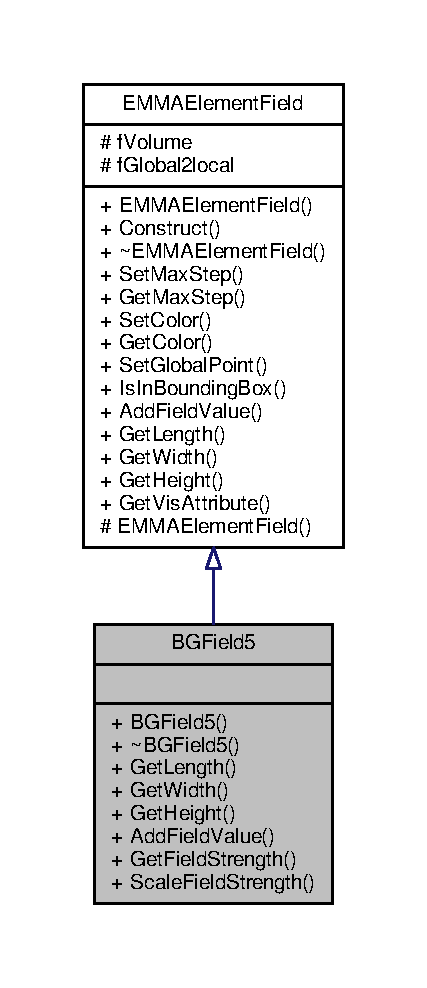
\includegraphics[width=205pt]{classBGField5__inherit__graph}
\end{center}
\end{figure}


Collaboration diagram for B\+G\+Field5\+:
\nopagebreak
\begin{figure}[H]
\begin{center}
\leavevmode
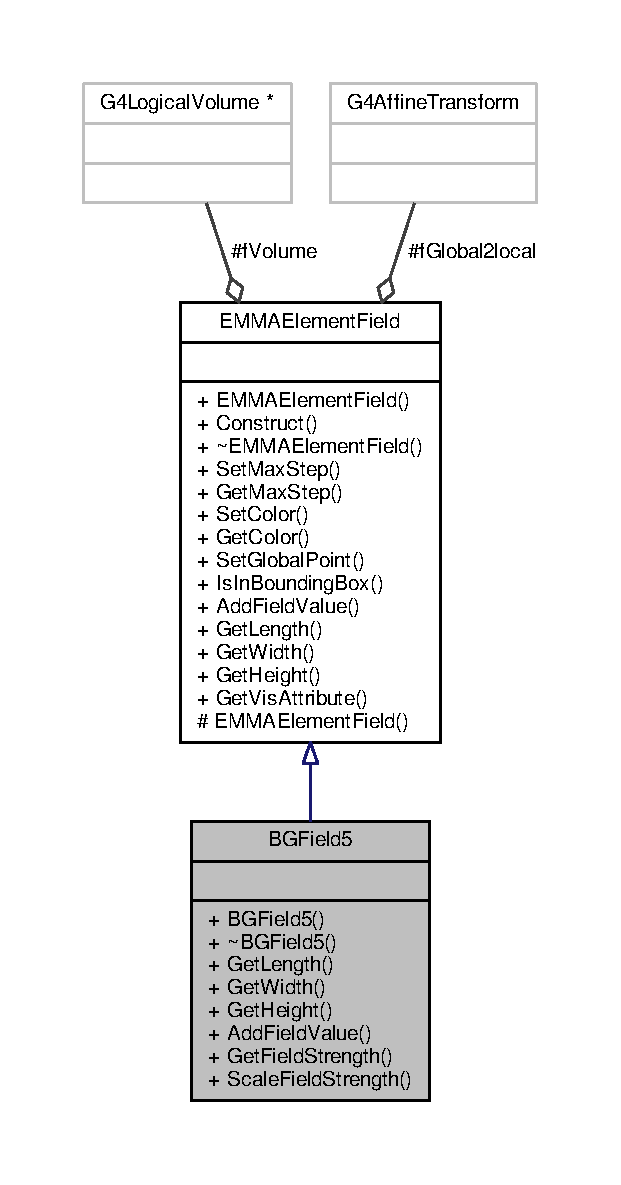
\includegraphics[height=550pt]{classBGField5__coll__graph}
\end{center}
\end{figure}
\subsection*{Public Member Functions}
\begin{DoxyCompactItemize}
\item 
\hyperlink{classBGField5_afe5dd17ba8949f419920c47952dbe10b}{B\+G\+Field5} (G4double xoffset, G4double zoffset, G4double zbefore, G4double zafter, G4\+Logical\+Volume $\ast$, G4\+Three\+Vector)
\item 
\hyperlink{classBGField5_abcbf36e1b0d700552977f55cd65eed2b}{$\sim$\+B\+G\+Field5} ()
\item 
virtual G4double \hyperlink{classBGField5_aa003bda3eb139d5c6f1bddbbc7ee9a3f}{Get\+Length} ()
\item 
virtual G4double \hyperlink{classBGField5_aca250c0313214b8ca38d47df1e1a45d2}{Get\+Width} ()
\item 
virtual G4double \hyperlink{classBGField5_ab9cdd6f73808a2e8cfc1ad14bc0ee4bb}{Get\+Height} ()
\item 
virtual void \hyperlink{classBGField5_a85ddce900e965338562cd7d6b28eb08d}{Add\+Field\+Value} (const G4double Point\mbox{[}3\mbox{]}, G4double field\mbox{[}6\mbox{]}) const 
\item 
G4double \hyperlink{classBGField5_a7fcafffe48960675096f1693203ae437}{Get\+Field\+Strength} ()
\item 
void \hyperlink{classBGField5_a3298d0794e6914bfebe6550a6b08ee26}{Scale\+Field\+Strength} (G4double esf)
\end{DoxyCompactItemize}
\subsection*{Additional Inherited Members}


\subsection{Constructor \& Destructor Documentation}
\index{B\+G\+Field5@{B\+G\+Field5}!B\+G\+Field5@{B\+G\+Field5}}
\index{B\+G\+Field5@{B\+G\+Field5}!B\+G\+Field5@{B\+G\+Field5}}
\subsubsection[{\texorpdfstring{B\+G\+Field5(\+G4double xoffset, G4double zoffset, G4double zbefore, G4double zafter, G4\+Logical\+Volume $\ast$, G4\+Three\+Vector)}{BGField5(G4double xoffset, G4double zoffset, G4double zbefore, G4double zafter, G4LogicalVolume *, G4ThreeVector)}}]{\setlength{\rightskip}{0pt plus 5cm}B\+G\+Field5\+::\+B\+G\+Field5 (
\begin{DoxyParamCaption}
\item[{G4double}]{xoffset, }
\item[{G4double}]{zoffset, }
\item[{G4double}]{zbefore, }
\item[{G4double}]{zafter, }
\item[{G4\+Logical\+Volume $\ast$}]{, }
\item[{G4\+Three\+Vector}]{}
\end{DoxyParamCaption}
)}\hypertarget{classBGField5_afe5dd17ba8949f419920c47952dbe10b}{}\label{classBGField5_afe5dd17ba8949f419920c47952dbe10b}
\index{B\+G\+Field5@{B\+G\+Field5}!````~B\+G\+Field5@{$\sim$\+B\+G\+Field5}}
\index{````~B\+G\+Field5@{$\sim$\+B\+G\+Field5}!B\+G\+Field5@{B\+G\+Field5}}
\subsubsection[{\texorpdfstring{$\sim$\+B\+G\+Field5()}{~BGField5()}}]{\setlength{\rightskip}{0pt plus 5cm}B\+G\+Field5\+::$\sim$\+B\+G\+Field5 (
\begin{DoxyParamCaption}
{}
\end{DoxyParamCaption}
)}\hypertarget{classBGField5_abcbf36e1b0d700552977f55cd65eed2b}{}\label{classBGField5_abcbf36e1b0d700552977f55cd65eed2b}


\subsection{Member Function Documentation}
\index{B\+G\+Field5@{B\+G\+Field5}!Add\+Field\+Value@{Add\+Field\+Value}}
\index{Add\+Field\+Value@{Add\+Field\+Value}!B\+G\+Field5@{B\+G\+Field5}}
\subsubsection[{\texorpdfstring{Add\+Field\+Value(const G4double Point[3], G4double field[6]) const }{AddFieldValue(const G4double Point[3], G4double field[6]) const }}]{\setlength{\rightskip}{0pt plus 5cm}virtual void B\+G\+Field5\+::\+Add\+Field\+Value (
\begin{DoxyParamCaption}
\item[{const G4double}]{Point\mbox{[}3\mbox{]}, }
\item[{G4double}]{field\mbox{[}6\mbox{]}}
\end{DoxyParamCaption}
) const\hspace{0.3cm}{\ttfamily [virtual]}}\hypertarget{classBGField5_a85ddce900e965338562cd7d6b28eb08d}{}\label{classBGField5_a85ddce900e965338562cd7d6b28eb08d}
\index{B\+G\+Field5@{B\+G\+Field5}!Get\+Field\+Strength@{Get\+Field\+Strength}}
\index{Get\+Field\+Strength@{Get\+Field\+Strength}!B\+G\+Field5@{B\+G\+Field5}}
\subsubsection[{\texorpdfstring{Get\+Field\+Strength()}{GetFieldStrength()}}]{\setlength{\rightskip}{0pt plus 5cm}G4double B\+G\+Field5\+::\+Get\+Field\+Strength (
\begin{DoxyParamCaption}
{}
\end{DoxyParamCaption}
)\hspace{0.3cm}{\ttfamily [inline]}}\hypertarget{classBGField5_a7fcafffe48960675096f1693203ae437}{}\label{classBGField5_a7fcafffe48960675096f1693203ae437}
\index{B\+G\+Field5@{B\+G\+Field5}!Get\+Height@{Get\+Height}}
\index{Get\+Height@{Get\+Height}!B\+G\+Field5@{B\+G\+Field5}}
\subsubsection[{\texorpdfstring{Get\+Height()}{GetHeight()}}]{\setlength{\rightskip}{0pt plus 5cm}virtual G4double B\+G\+Field5\+::\+Get\+Height (
\begin{DoxyParamCaption}
{}
\end{DoxyParamCaption}
)\hspace{0.3cm}{\ttfamily [inline]}, {\ttfamily [virtual]}}\hypertarget{classBGField5_ab9cdd6f73808a2e8cfc1ad14bc0ee4bb}{}\label{classBGField5_ab9cdd6f73808a2e8cfc1ad14bc0ee4bb}


Implements \hyperlink{classEMMAElementField_a3cbd223805ba24b5313e16ca540c326c}{E\+M\+M\+A\+Element\+Field}.

\index{B\+G\+Field5@{B\+G\+Field5}!Get\+Length@{Get\+Length}}
\index{Get\+Length@{Get\+Length}!B\+G\+Field5@{B\+G\+Field5}}
\subsubsection[{\texorpdfstring{Get\+Length()}{GetLength()}}]{\setlength{\rightskip}{0pt plus 5cm}virtual G4double B\+G\+Field5\+::\+Get\+Length (
\begin{DoxyParamCaption}
{}
\end{DoxyParamCaption}
)\hspace{0.3cm}{\ttfamily [inline]}, {\ttfamily [virtual]}}\hypertarget{classBGField5_aa003bda3eb139d5c6f1bddbbc7ee9a3f}{}\label{classBGField5_aa003bda3eb139d5c6f1bddbbc7ee9a3f}


Implements \hyperlink{classEMMAElementField_adb2d90c3fdf25e17be541903bffca35b}{E\+M\+M\+A\+Element\+Field}.

\index{B\+G\+Field5@{B\+G\+Field5}!Get\+Width@{Get\+Width}}
\index{Get\+Width@{Get\+Width}!B\+G\+Field5@{B\+G\+Field5}}
\subsubsection[{\texorpdfstring{Get\+Width()}{GetWidth()}}]{\setlength{\rightskip}{0pt plus 5cm}virtual G4double B\+G\+Field5\+::\+Get\+Width (
\begin{DoxyParamCaption}
{}
\end{DoxyParamCaption}
)\hspace{0.3cm}{\ttfamily [inline]}, {\ttfamily [virtual]}}\hypertarget{classBGField5_aca250c0313214b8ca38d47df1e1a45d2}{}\label{classBGField5_aca250c0313214b8ca38d47df1e1a45d2}


Implements \hyperlink{classEMMAElementField_a41708a8f1e72d7788c0a53c80c297bf9}{E\+M\+M\+A\+Element\+Field}.

\index{B\+G\+Field5@{B\+G\+Field5}!Scale\+Field\+Strength@{Scale\+Field\+Strength}}
\index{Scale\+Field\+Strength@{Scale\+Field\+Strength}!B\+G\+Field5@{B\+G\+Field5}}
\subsubsection[{\texorpdfstring{Scale\+Field\+Strength(\+G4double esf)}{ScaleFieldStrength(G4double esf)}}]{\setlength{\rightskip}{0pt plus 5cm}void B\+G\+Field5\+::\+Scale\+Field\+Strength (
\begin{DoxyParamCaption}
\item[{G4double}]{esf}
\end{DoxyParamCaption}
)\hspace{0.3cm}{\ttfamily [inline]}}\hypertarget{classBGField5_a3298d0794e6914bfebe6550a6b08ee26}{}\label{classBGField5_a3298d0794e6914bfebe6550a6b08ee26}


The documentation for this class was generated from the following file\+:\begin{DoxyCompactItemize}
\item 
\hyperlink{BGField5_8hh}{B\+G\+Field5.\+hh}\end{DoxyCompactItemize}

\hypertarget{classBGField6}{\section{B\-G\-Field6 Class Reference}
\label{classBGField6}\index{B\-G\-Field6@{B\-G\-Field6}}
}
Inheritance diagram for B\-G\-Field6\-:\begin{figure}[H]
\begin{center}
\leavevmode
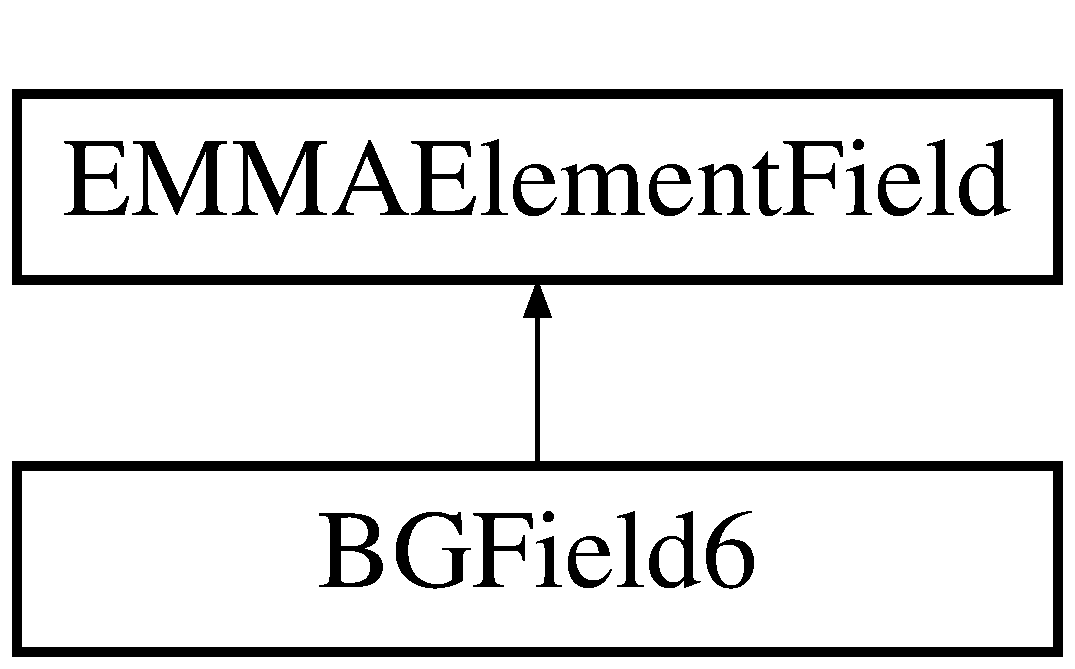
\includegraphics[height=2.000000cm]{classBGField6}
\end{center}
\end{figure}
\subsection*{Public Member Functions}
\begin{DoxyCompactItemize}
\item 
\hypertarget{classBGField6_a6f02a8a1e9643d6177d5f3f30d7a46e0}{{\bfseries B\-G\-Field6} (G4double xoffset, G4double zoffset, G4double zbefore, G4double zafter, G4\-Logical\-Volume $\ast$, G4\-Three\-Vector)}\label{classBGField6_a6f02a8a1e9643d6177d5f3f30d7a46e0}

\item 
\hypertarget{classBGField6_ae0703e3eeb230040b028aaae44b2f2a4}{virtual G4double {\bfseries Get\-Length} ()}\label{classBGField6_ae0703e3eeb230040b028aaae44b2f2a4}

\item 
\hypertarget{classBGField6_a620f1dfb4e72bf4cd8156eff68f4359a}{virtual G4double {\bfseries Get\-Width} ()}\label{classBGField6_a620f1dfb4e72bf4cd8156eff68f4359a}

\item 
\hypertarget{classBGField6_a47b7a214491b4317706fcd61d0f9feef}{virtual G4double {\bfseries Get\-Height} ()}\label{classBGField6_a47b7a214491b4317706fcd61d0f9feef}

\item 
\hypertarget{classBGField6_aaacc495750db2c0672cc4c7be39a6c8c}{virtual void {\bfseries Add\-Field\-Value} (const G4double Point\mbox{[}3\mbox{]}, G4double field\mbox{[}6\mbox{]}) const }\label{classBGField6_aaacc495750db2c0672cc4c7be39a6c8c}

\item 
\hypertarget{classBGField6_a4af95bf2bc47babe4c29f814bb8afa1c}{G4double {\bfseries Get\-Field\-Strength} ()}\label{classBGField6_a4af95bf2bc47babe4c29f814bb8afa1c}

\item 
\hypertarget{classBGField6_a8045ecf2de2401570f87f72270875b72}{void {\bfseries Scale\-Field\-Strength} (G4double msf)}\label{classBGField6_a8045ecf2de2401570f87f72270875b72}

\end{DoxyCompactItemize}
\subsection*{Additional Inherited Members}


The documentation for this class was generated from the following file\-:\begin{DoxyCompactItemize}
\item 
\hyperlink{BGField6_8hh}{B\-G\-Field6.\-hh}\end{DoxyCompactItemize}

\hypertarget{classBGField7}{\section{B\-G\-Field7 Class Reference}
\label{classBGField7}\index{B\-G\-Field7@{B\-G\-Field7}}
}
Inheritance diagram for B\-G\-Field7\-:\begin{figure}[H]
\begin{center}
\leavevmode
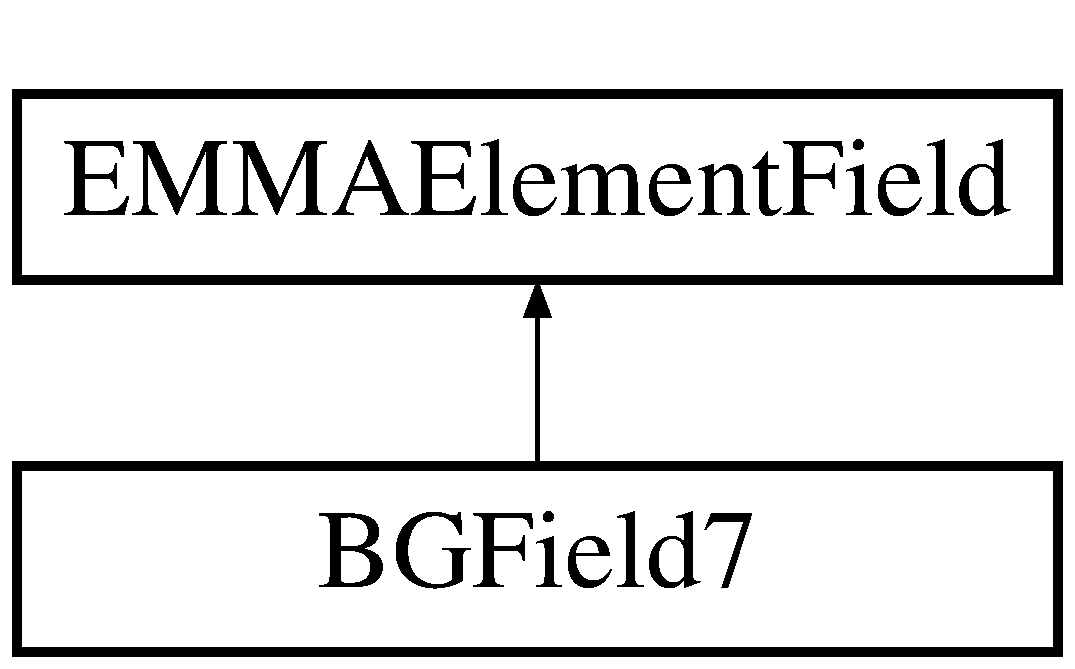
\includegraphics[height=2.000000cm]{classBGField7}
\end{center}
\end{figure}
\subsection*{Public Member Functions}
\begin{DoxyCompactItemize}
\item 
\hypertarget{classBGField7_a7a8a66516a7c721f5bbc537a11c74611}{{\bfseries B\-G\-Field7} (G4double xoffset, G4double zoffset, G4double zbefore, G4double zafter, G4\-Logical\-Volume $\ast$, G4\-Three\-Vector)}\label{classBGField7_a7a8a66516a7c721f5bbc537a11c74611}

\item 
\hypertarget{classBGField7_a4a490c55acab01b0fdd558ed8117c20d}{virtual G4double {\bfseries Get\-Length} ()}\label{classBGField7_a4a490c55acab01b0fdd558ed8117c20d}

\item 
\hypertarget{classBGField7_a26a7446a2a71f53d7e6562636cbd6dec}{virtual G4double {\bfseries Get\-Width} ()}\label{classBGField7_a26a7446a2a71f53d7e6562636cbd6dec}

\item 
\hypertarget{classBGField7_af997fdbf9563607d88ea8846674054f0}{virtual G4double {\bfseries Get\-Height} ()}\label{classBGField7_af997fdbf9563607d88ea8846674054f0}

\item 
\hypertarget{classBGField7_ace0f21a51ad1076f9cc7fc4558ee2ef7}{virtual void {\bfseries Add\-Field\-Value} (const G4double Point\mbox{[}3\mbox{]}, G4double field\mbox{[}6\mbox{]}) const }\label{classBGField7_ace0f21a51ad1076f9cc7fc4558ee2ef7}

\item 
\hypertarget{classBGField7_a504c09a6ed73181e1131e745817d80e1}{G4double {\bfseries Get\-Field\-Strength} ()}\label{classBGField7_a504c09a6ed73181e1131e745817d80e1}

\item 
\hypertarget{classBGField7_af175b7fc74bed2669bfb3036d6475dbb}{void {\bfseries Scale\-Field\-Strength} (G4double msf)}\label{classBGField7_af175b7fc74bed2669bfb3036d6475dbb}

\end{DoxyCompactItemize}
\subsection*{Additional Inherited Members}


The documentation for this class was generated from the following file\-:\begin{DoxyCompactItemize}
\item 
\hyperlink{BGField7_8hh}{B\-G\-Field7.\-hh}\end{DoxyCompactItemize}

\hypertarget{classc2__arrhenius__function__transformation}{\section{c2\-\_\-arrhenius\-\_\-function\-\_\-transformation$<$ float\-\_\-type $>$ Class Template Reference}
\label{classc2__arrhenius__function__transformation}\index{c2\-\_\-arrhenius\-\_\-function\-\_\-transformation$<$ float\-\_\-type $>$@{c2\-\_\-arrhenius\-\_\-function\-\_\-transformation$<$ float\-\_\-type $>$}}
}


a transformation of a function in and out of Arrhenius (1/x vs. log(y)) space  




{\ttfamily \#include $<$c2\-\_\-function.\-hh$>$}

Inheritance diagram for c2\-\_\-arrhenius\-\_\-function\-\_\-transformation$<$ float\-\_\-type $>$\-:\begin{figure}[H]
\begin{center}
\leavevmode
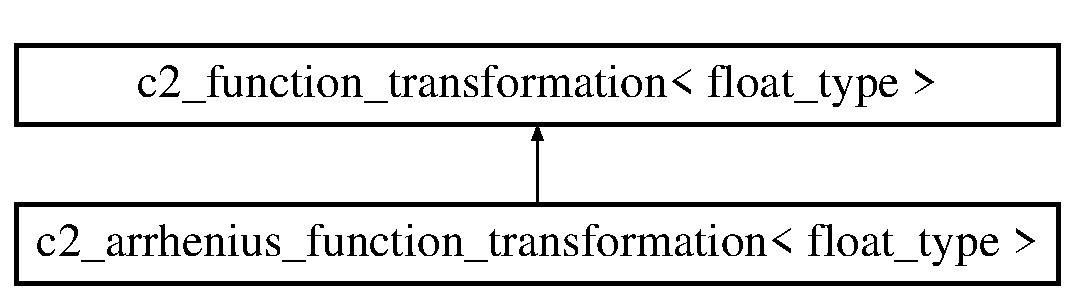
\includegraphics[height=2.000000cm]{classc2__arrhenius__function__transformation}
\end{center}
\end{figure}
\subsection*{Additional Inherited Members}


\subsection{Detailed Description}
\subsubsection*{template$<$typename float\-\_\-type$>$class c2\-\_\-arrhenius\-\_\-function\-\_\-transformation$<$ float\-\_\-type $>$}

a transformation of a function in and out of Arrhenius (1/x vs. log(y)) space 



The documentation for this class was generated from the following file\-:\begin{DoxyCompactItemize}
\item 
\hyperlink{c2__function_8hh}{c2\-\_\-function.\-hh}\end{DoxyCompactItemize}

\hypertarget{classc2__binary__function}{}\section{c2\+\_\+binary\+\_\+function$<$ float\+\_\+type $>$ Class Template Reference}
\label{classc2__binary__function}\index{c2\+\_\+binary\+\_\+function$<$ float\+\_\+type $>$@{c2\+\_\+binary\+\_\+function$<$ float\+\_\+type $>$}}


Provides support for \hyperlink{classc2__function}{c2\+\_\+function} objects which are constructed from two other \hyperlink{classc2__function}{c2\+\_\+function} objects.  




{\ttfamily \#include \char`\"{}c2\+\_\+function.\+hh\char`\"{}}



Inheritance diagram for c2\+\_\+binary\+\_\+function$<$ float\+\_\+type $>$\+:
\nopagebreak
\begin{figure}[H]
\begin{center}
\leavevmode
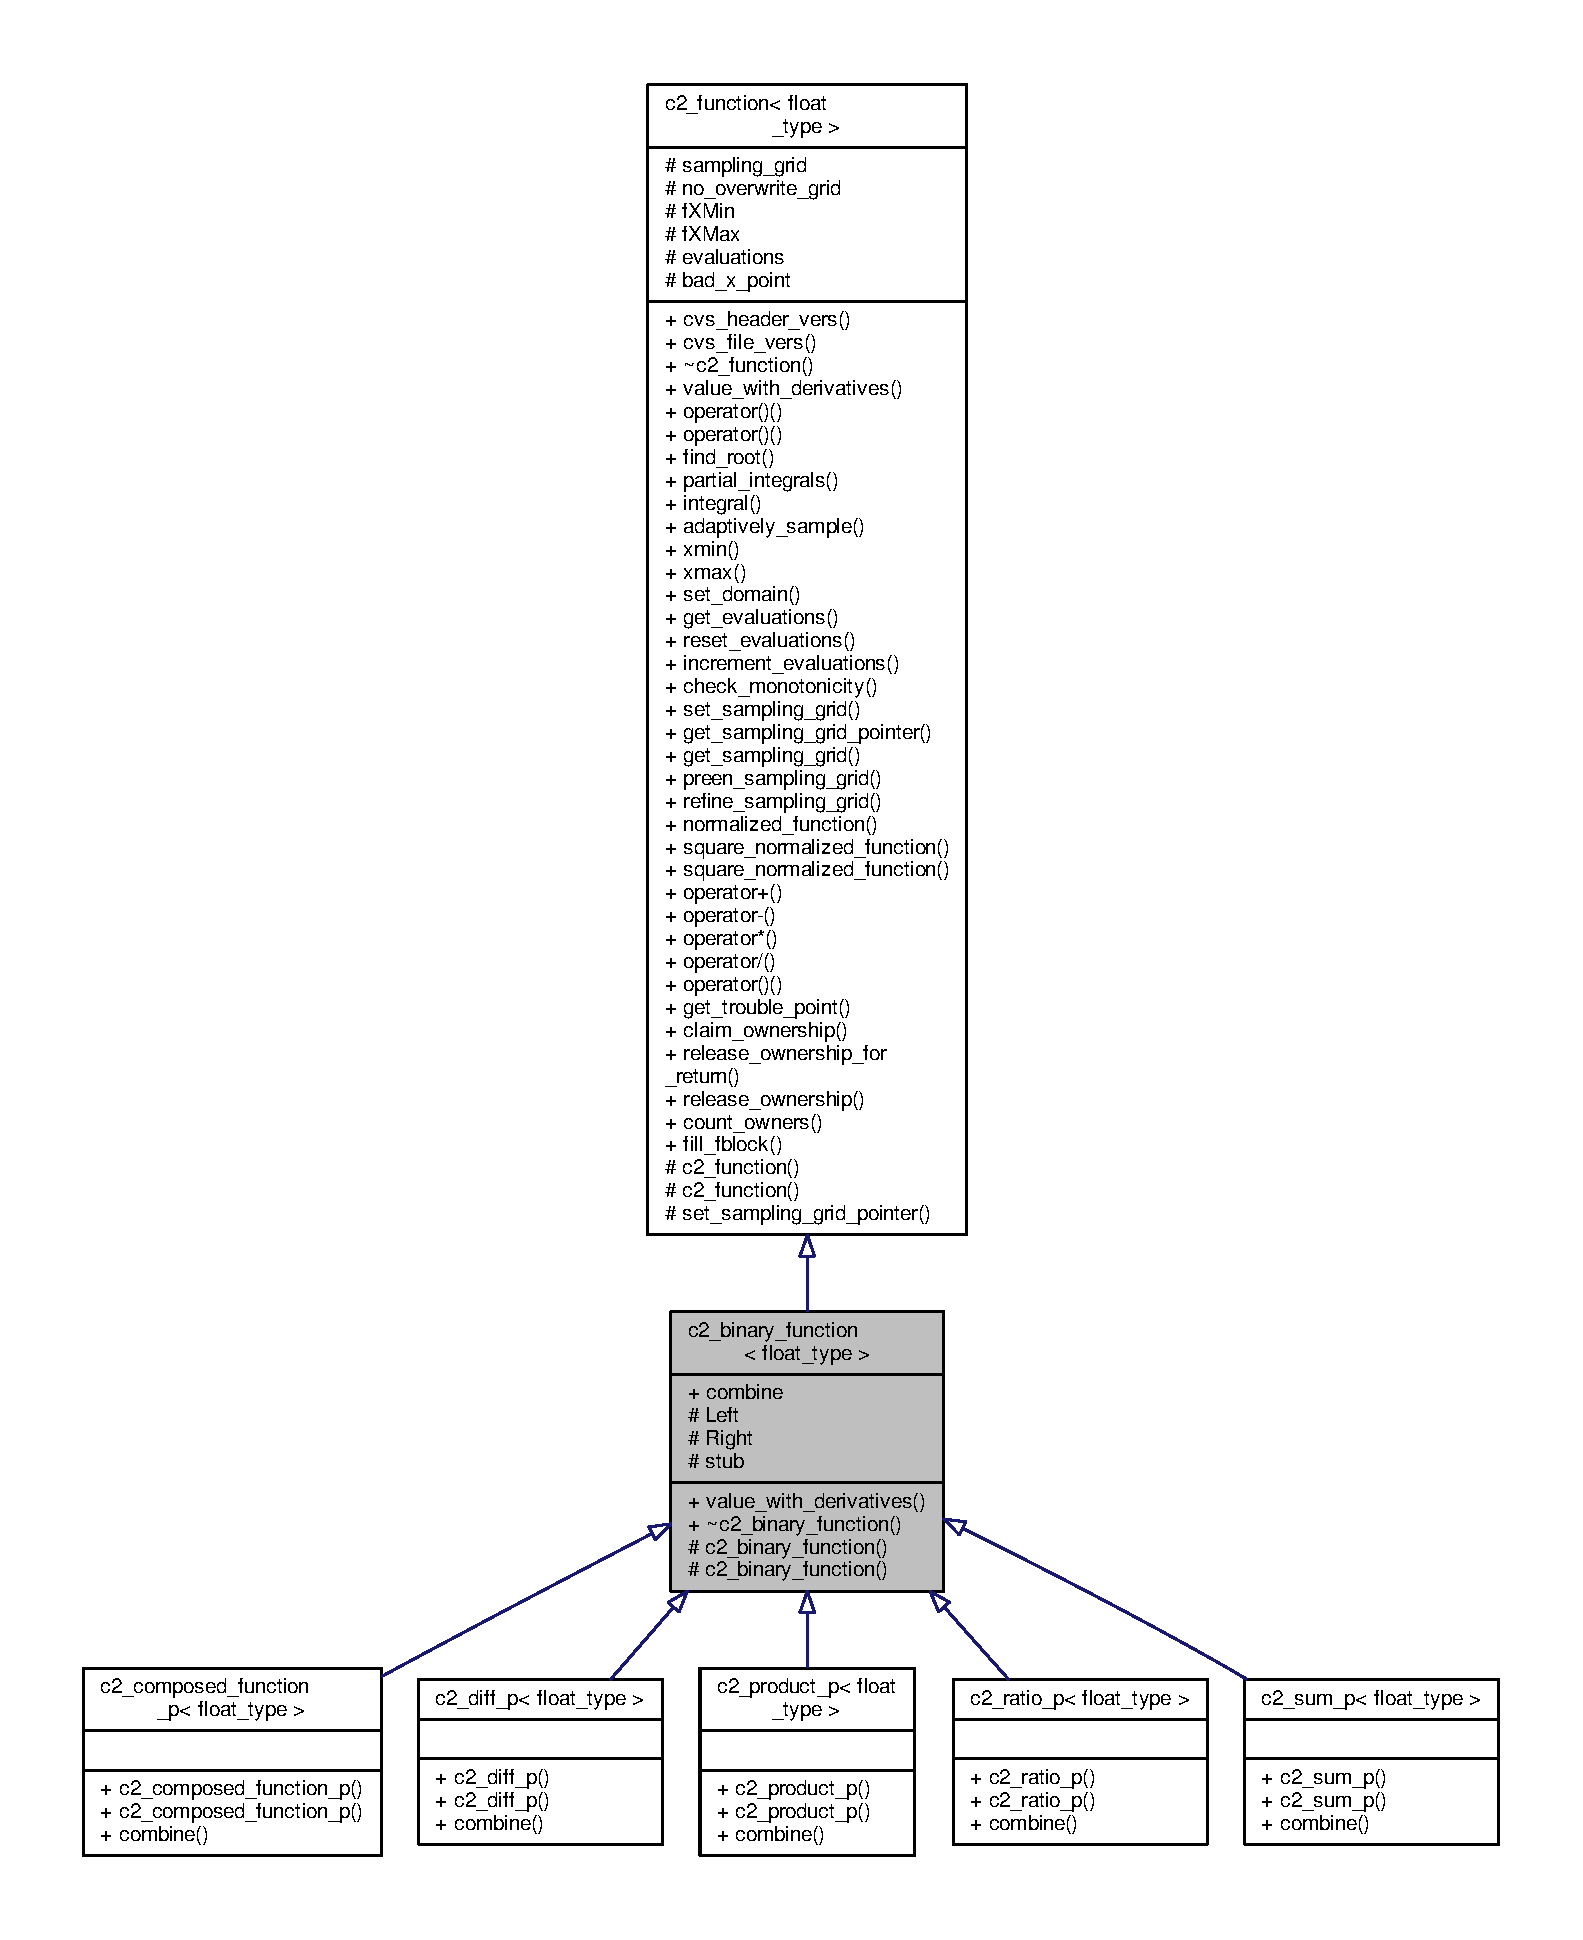
\includegraphics[width=350pt]{classc2__binary__function__inherit__graph}
\end{center}
\end{figure}


Collaboration diagram for c2\+\_\+binary\+\_\+function$<$ float\+\_\+type $>$\+:
\nopagebreak
\begin{figure}[H]
\begin{center}
\leavevmode
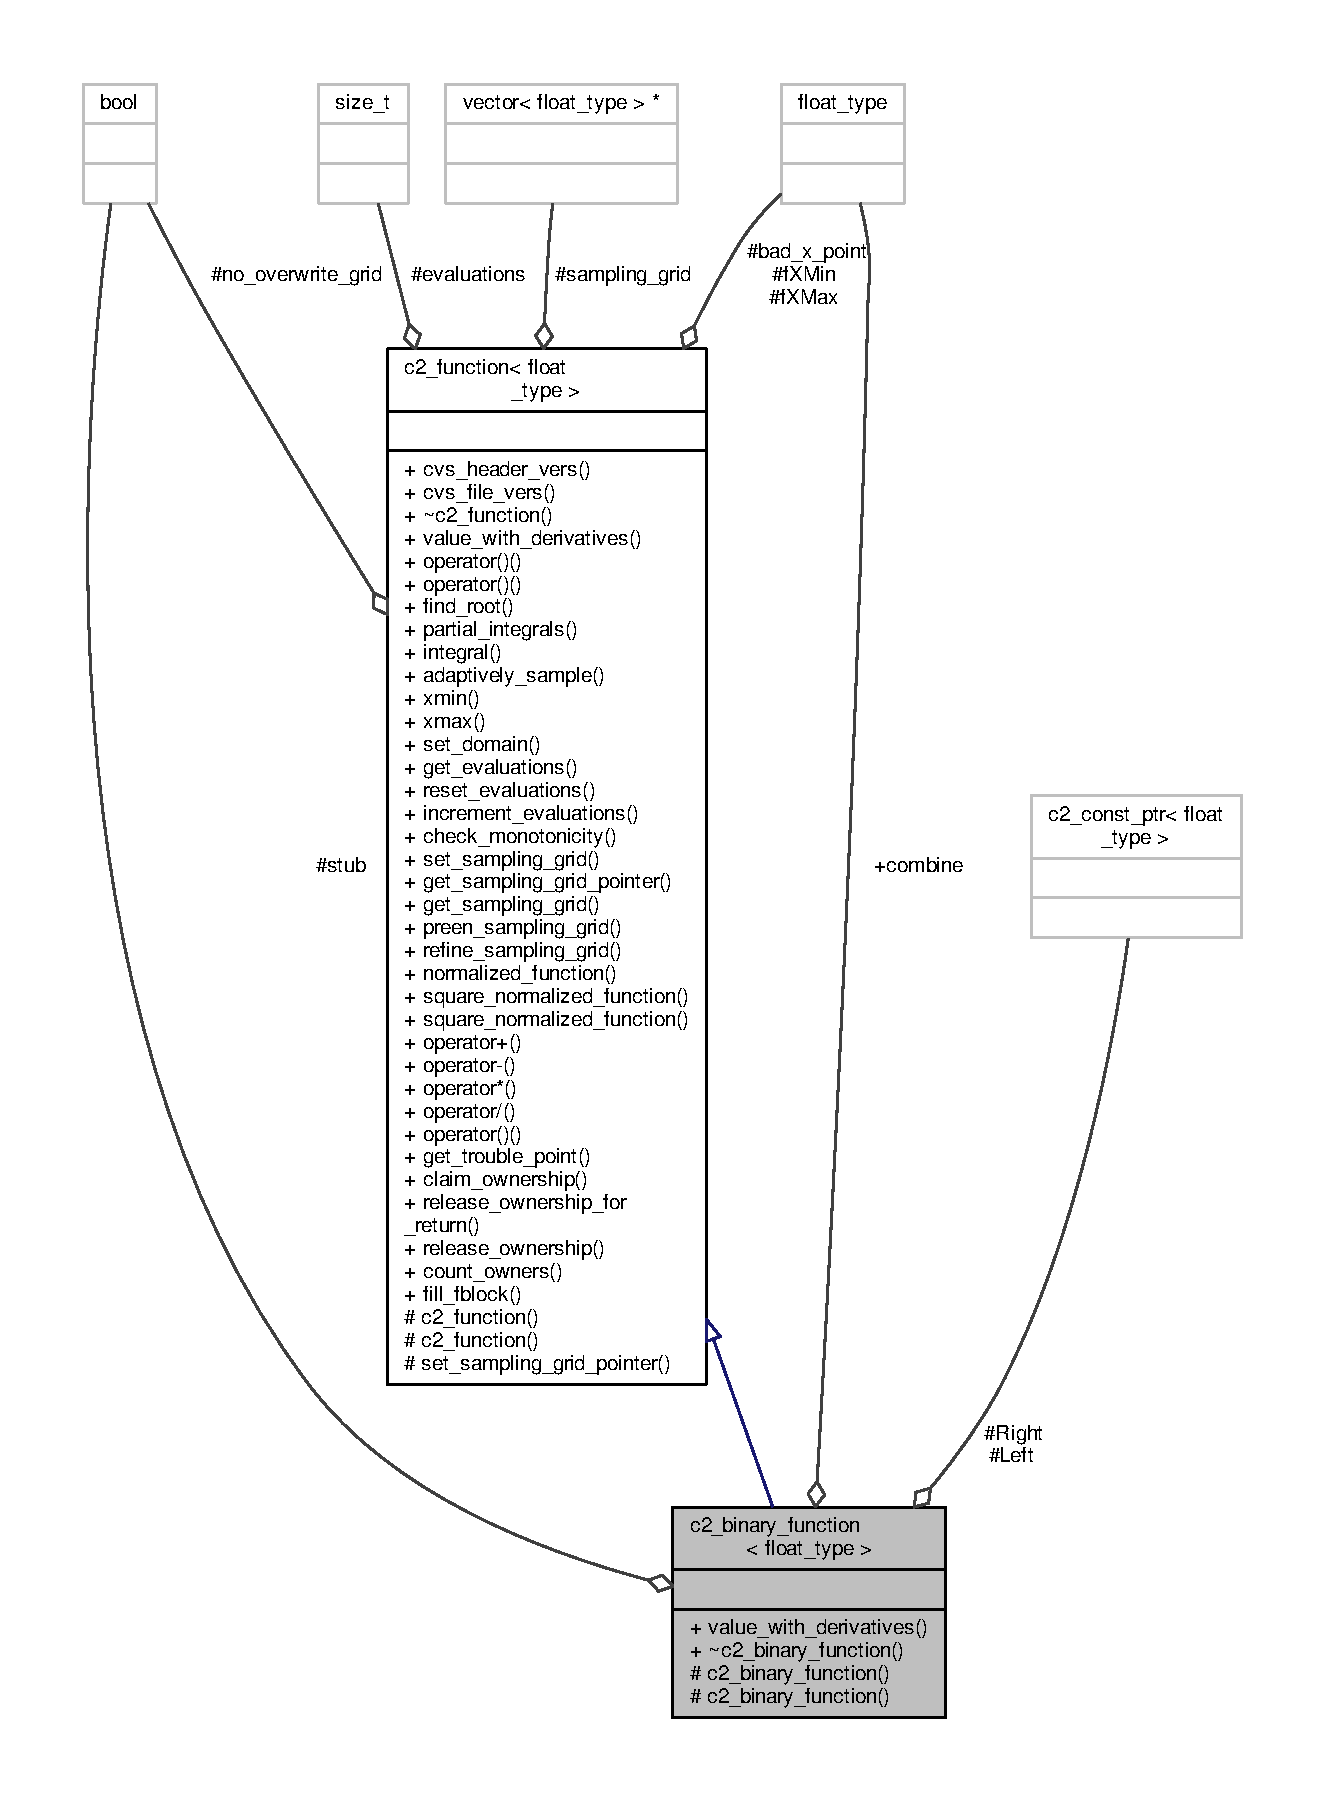
\includegraphics[width=350pt]{classc2__binary__function__coll__graph}
\end{center}
\end{figure}
\subsection*{Public Member Functions}
\begin{DoxyCompactItemize}
\item 
virtual float\+\_\+type \hyperlink{classc2__binary__function_a7ab60d022222ce65e99f8708bf2aae0d}{value\+\_\+with\+\_\+derivatives} (float\+\_\+type x, float\+\_\+type $\ast$yprime, float\+\_\+type $\ast$yprime2) const   throw (c2\+\_\+exception)
\begin{DoxyCompactList}\small\item\em function to manage the binary operation, used by \hyperlink{classc2__binary__function_a7ab60d022222ce65e99f8708bf2aae0d}{c2\+\_\+binary\+\_\+function\+::value\+\_\+with\+\_\+derivatives()} \end{DoxyCompactList}\item 
virtual \hyperlink{classc2__binary__function_aaec2d1f2a53845f36974b0b82786d4f2}{$\sim$c2\+\_\+binary\+\_\+function} ()
\begin{DoxyCompactList}\small\item\em destructor releases ownership of member functions \end{DoxyCompactList}\end{DoxyCompactItemize}
\subsection*{Public Attributes}
\begin{DoxyCompactItemize}
\item 
float\+\_\+type($\ast$const \hyperlink{classc2__binary__function_a03189b157a02b97b2f885196616c01a0}{combine} )(const \hyperlink{classc2__function}{c2\+\_\+function}$<$ float\+\_\+type $>$ \&left, const \hyperlink{classc2__function}{c2\+\_\+function}$<$ float\+\_\+type $>$ \&right, float\+\_\+type x, float\+\_\+type $\ast$yprime, float\+\_\+type $\ast$yprime2)
\end{DoxyCompactItemize}
\subsection*{Protected Member Functions}
\begin{DoxyCompactItemize}
\item 
\hyperlink{classc2__binary__function_a1daf580ba04ae495309f9c83bd615f68}{c2\+\_\+binary\+\_\+function} (float\+\_\+type($\ast$combiner)(const \hyperlink{classc2__function}{c2\+\_\+function}$<$ float\+\_\+type $>$ \&left, const \hyperlink{classc2__function}{c2\+\_\+function}$<$ float\+\_\+type $>$ \&right, float\+\_\+type x, float\+\_\+type $\ast$yprime, float\+\_\+type $\ast$yprime2), const \hyperlink{classc2__function}{c2\+\_\+function}$<$ float\+\_\+type $>$ \&left, const \hyperlink{classc2__function}{c2\+\_\+function}$<$ float\+\_\+type $>$ \&right)
\begin{DoxyCompactList}\small\item\em construct the binary function \end{DoxyCompactList}\item 
\hyperlink{classc2__binary__function_a99809843f818ae9c451a0339b0f46bdc}{c2\+\_\+binary\+\_\+function} (float\+\_\+type($\ast$combiner)(const \hyperlink{classc2__function}{c2\+\_\+function}$<$ float\+\_\+type $>$ \&left, const \hyperlink{classc2__function}{c2\+\_\+function}$<$ float\+\_\+type $>$ \&right, float\+\_\+type x, float\+\_\+type $\ast$yprime, float\+\_\+type $\ast$yprime2))
\begin{DoxyCompactList}\small\item\em construct a \textquotesingle{}stub\textquotesingle{} \hyperlink{classc2__binary__function}{c2\+\_\+binary\+\_\+function}, which provides access to the \hyperlink{classc2__binary__function_a03189b157a02b97b2f885196616c01a0}{combine()} function \end{DoxyCompactList}\end{DoxyCompactItemize}
\subsection*{Protected Attributes}
\begin{DoxyCompactItemize}
\item 
const \hyperlink{classc2__const__ptr}{c2\+\_\+const\+\_\+ptr}$<$ float\+\_\+type $>$ \hyperlink{classc2__binary__function_a53d43543e7057fe762fd14ae58ac327a}{Left}
\item 
const \hyperlink{classc2__const__ptr}{c2\+\_\+const\+\_\+ptr}$<$ float\+\_\+type $>$ \hyperlink{classc2__binary__function_a52b7fcaed6a4c3e3146dea43f562db8d}{Right}
\item 
bool \hyperlink{classc2__binary__function_a7d6abdb0e7fcfb4fd65833a42f93c561}{stub}
\begin{DoxyCompactList}\small\item\em if true, we don\textquotesingle{}t own any functions, we are just a source of a combining function. \end{DoxyCompactList}\end{DoxyCompactItemize}


\subsection{Detailed Description}
\subsubsection*{template$<$typename float\+\_\+type = double$>$\\*
class c2\+\_\+binary\+\_\+function$<$ float\+\_\+type $>$}

Provides support for \hyperlink{classc2__function}{c2\+\_\+function} objects which are constructed from two other \hyperlink{classc2__function}{c2\+\_\+function} objects. 

\subsection{Constructor \& Destructor Documentation}
\index{c2\+\_\+binary\+\_\+function@{c2\+\_\+binary\+\_\+function}!````~c2\+\_\+binary\+\_\+function@{$\sim$c2\+\_\+binary\+\_\+function}}
\index{````~c2\+\_\+binary\+\_\+function@{$\sim$c2\+\_\+binary\+\_\+function}!c2\+\_\+binary\+\_\+function@{c2\+\_\+binary\+\_\+function}}
\subsubsection[{\texorpdfstring{$\sim$c2\+\_\+binary\+\_\+function()}{~c2_binary_function()}}]{\setlength{\rightskip}{0pt plus 5cm}template$<$typename float\+\_\+type = double$>$ virtual {\bf c2\+\_\+binary\+\_\+function}$<$ float\+\_\+type $>$\+::$\sim${\bf c2\+\_\+binary\+\_\+function} (
\begin{DoxyParamCaption}
{}
\end{DoxyParamCaption}
)\hspace{0.3cm}{\ttfamily [inline]}, {\ttfamily [virtual]}}\hypertarget{classc2__binary__function_aaec2d1f2a53845f36974b0b82786d4f2}{}\label{classc2__binary__function_aaec2d1f2a53845f36974b0b82786d4f2}


destructor releases ownership of member functions 

\index{c2\+\_\+binary\+\_\+function@{c2\+\_\+binary\+\_\+function}!c2\+\_\+binary\+\_\+function@{c2\+\_\+binary\+\_\+function}}
\index{c2\+\_\+binary\+\_\+function@{c2\+\_\+binary\+\_\+function}!c2\+\_\+binary\+\_\+function@{c2\+\_\+binary\+\_\+function}}
\subsubsection[{\texorpdfstring{c2\+\_\+binary\+\_\+function(float\+\_\+type($\ast$combiner)(const c2\+\_\+function$<$ float\+\_\+type $>$ \&left, const c2\+\_\+function$<$ float\+\_\+type $>$ \&right, float\+\_\+type x, float\+\_\+type $\ast$yprime, float\+\_\+type $\ast$yprime2), const c2\+\_\+function$<$ float\+\_\+type $>$ \&left, const c2\+\_\+function$<$ float\+\_\+type $>$ \&right)}{c2_binary_function(float_type(*combiner)(const c2_function< float_type > &left, const c2_function< float_type > &right, float_type x, float_type *yprime, float_type *yprime2), const c2_function< float_type > &left, const c2_function< float_type > &right)}}]{\setlength{\rightskip}{0pt plus 5cm}template$<$typename float\+\_\+type = double$>$ {\bf c2\+\_\+binary\+\_\+function}$<$ float\+\_\+type $>$\+::{\bf c2\+\_\+binary\+\_\+function} (
\begin{DoxyParamCaption}
\item[{float\+\_\+type($\ast$)(const {\bf c2\+\_\+function}$<$ float\+\_\+type $>$ \&left, const {\bf c2\+\_\+function}$<$ float\+\_\+type $>$ \&right, float\+\_\+type x, float\+\_\+type $\ast$yprime, float\+\_\+type $\ast$yprime2)}]{combiner, }
\item[{const {\bf c2\+\_\+function}$<$ float\+\_\+type $>$ \&}]{left, }
\item[{const {\bf c2\+\_\+function}$<$ float\+\_\+type $>$ \&}]{right}
\end{DoxyParamCaption}
)\hspace{0.3cm}{\ttfamily [inline]}, {\ttfamily [protected]}}\hypertarget{classc2__binary__function_a1daf580ba04ae495309f9c83bd615f68}{}\label{classc2__binary__function_a1daf580ba04ae495309f9c83bd615f68}


construct the binary function 


\begin{DoxyParams}{Parameters}
{\em combiner} & pointer to the function which actualy knows how to execute the binary \\
\hline
{\em left} & the \hyperlink{classc2__function}{c2\+\_\+function} to be used in the left side of the binary relation \\
\hline
{\em right} & the \hyperlink{classc2__function}{c2\+\_\+function} to be used in the right side of the binary relation \\
\hline
\end{DoxyParams}
\index{c2\+\_\+binary\+\_\+function@{c2\+\_\+binary\+\_\+function}!c2\+\_\+binary\+\_\+function@{c2\+\_\+binary\+\_\+function}}
\index{c2\+\_\+binary\+\_\+function@{c2\+\_\+binary\+\_\+function}!c2\+\_\+binary\+\_\+function@{c2\+\_\+binary\+\_\+function}}
\subsubsection[{\texorpdfstring{c2\+\_\+binary\+\_\+function(float\+\_\+type($\ast$combiner)(const c2\+\_\+function$<$ float\+\_\+type $>$ \&left, const c2\+\_\+function$<$ float\+\_\+type $>$ \&right, float\+\_\+type x, float\+\_\+type $\ast$yprime, float\+\_\+type $\ast$yprime2))}{c2_binary_function(float_type(*combiner)(const c2_function< float_type > &left, const c2_function< float_type > &right, float_type x, float_type *yprime, float_type *yprime2))}}]{\setlength{\rightskip}{0pt plus 5cm}template$<$typename float\+\_\+type = double$>$ {\bf c2\+\_\+binary\+\_\+function}$<$ float\+\_\+type $>$\+::{\bf c2\+\_\+binary\+\_\+function} (
\begin{DoxyParamCaption}
\item[{float\+\_\+type($\ast$)(const {\bf c2\+\_\+function}$<$ float\+\_\+type $>$ \&left, const {\bf c2\+\_\+function}$<$ float\+\_\+type $>$ \&right, float\+\_\+type x, float\+\_\+type $\ast$yprime, float\+\_\+type $\ast$yprime2)}]{combiner}
\end{DoxyParamCaption}
)\hspace{0.3cm}{\ttfamily [inline]}, {\ttfamily [protected]}}\hypertarget{classc2__binary__function_a99809843f818ae9c451a0339b0f46bdc}{}\label{classc2__binary__function_a99809843f818ae9c451a0339b0f46bdc}


construct a \textquotesingle{}stub\textquotesingle{} \hyperlink{classc2__binary__function}{c2\+\_\+binary\+\_\+function}, which provides access to the \hyperlink{classc2__binary__function_a03189b157a02b97b2f885196616c01a0}{combine()} function 

\begin{DoxyNote}{Note}
Do not evaluate a \textquotesingle{}stub\textquotesingle{} ever. It is only used so that \hyperlink{classc2__binary__function_a03189b157a02b97b2f885196616c01a0}{combine()} can be called 
\end{DoxyNote}


\subsection{Member Function Documentation}
\index{c2\+\_\+binary\+\_\+function@{c2\+\_\+binary\+\_\+function}!value\+\_\+with\+\_\+derivatives@{value\+\_\+with\+\_\+derivatives}}
\index{value\+\_\+with\+\_\+derivatives@{value\+\_\+with\+\_\+derivatives}!c2\+\_\+binary\+\_\+function@{c2\+\_\+binary\+\_\+function}}
\subsubsection[{\texorpdfstring{value\+\_\+with\+\_\+derivatives(float\+\_\+type x, float\+\_\+type $\ast$yprime, float\+\_\+type $\ast$yprime2) const }{value_with_derivatives(float_type x, float_type *yprime, float_type *yprime2) const }}]{\setlength{\rightskip}{0pt plus 5cm}template$<$typename float\+\_\+type = double$>$ virtual float\+\_\+type {\bf c2\+\_\+binary\+\_\+function}$<$ float\+\_\+type $>$\+::value\+\_\+with\+\_\+derivatives (
\begin{DoxyParamCaption}
\item[{float\+\_\+type}]{x, }
\item[{float\+\_\+type $\ast$}]{yprime, }
\item[{float\+\_\+type $\ast$}]{yprime2}
\end{DoxyParamCaption}
) const throw  {\bf c2\+\_\+exception}) \hspace{0.3cm}{\ttfamily [inline]}, {\ttfamily [virtual]}}\hypertarget{classc2__binary__function_a7ab60d022222ce65e99f8708bf2aae0d}{}\label{classc2__binary__function_a7ab60d022222ce65e99f8708bf2aae0d}


function to manage the binary operation, used by \hyperlink{classc2__binary__function_a7ab60d022222ce65e99f8708bf2aae0d}{c2\+\_\+binary\+\_\+function\+::value\+\_\+with\+\_\+derivatives()} 



Implements \hyperlink{classc2__function_a44e0201159111350be7f746fc9026f67}{c2\+\_\+function$<$ float\+\_\+type $>$}.



\subsection{Member Data Documentation}
\index{c2\+\_\+binary\+\_\+function@{c2\+\_\+binary\+\_\+function}!combine@{combine}}
\index{combine@{combine}!c2\+\_\+binary\+\_\+function@{c2\+\_\+binary\+\_\+function}}
\subsubsection[{\texorpdfstring{combine}{combine}}]{\setlength{\rightskip}{0pt plus 5cm}template$<$typename float\+\_\+type = double$>$ float\+\_\+type($\ast$ const {\bf c2\+\_\+binary\+\_\+function}$<$ float\+\_\+type $>$\+::combine) (const {\bf c2\+\_\+function}$<$ float\+\_\+type $>$ \&left, const {\bf c2\+\_\+function}$<$ float\+\_\+type $>$ \&right, float\+\_\+type x, float\+\_\+type $\ast$yprime, float\+\_\+type $\ast$yprime2)}\hypertarget{classc2__binary__function_a03189b157a02b97b2f885196616c01a0}{}\label{classc2__binary__function_a03189b157a02b97b2f885196616c01a0}
\index{c2\+\_\+binary\+\_\+function@{c2\+\_\+binary\+\_\+function}!Left@{Left}}
\index{Left@{Left}!c2\+\_\+binary\+\_\+function@{c2\+\_\+binary\+\_\+function}}
\subsubsection[{\texorpdfstring{Left}{Left}}]{\setlength{\rightskip}{0pt plus 5cm}template$<$typename float\+\_\+type = double$>$ const {\bf c2\+\_\+const\+\_\+ptr}$<$float\+\_\+type$>$ {\bf c2\+\_\+binary\+\_\+function}$<$ float\+\_\+type $>$\+::Left\hspace{0.3cm}{\ttfamily [protected]}}\hypertarget{classc2__binary__function_a53d43543e7057fe762fd14ae58ac327a}{}\label{classc2__binary__function_a53d43543e7057fe762fd14ae58ac327a}
\index{c2\+\_\+binary\+\_\+function@{c2\+\_\+binary\+\_\+function}!Right@{Right}}
\index{Right@{Right}!c2\+\_\+binary\+\_\+function@{c2\+\_\+binary\+\_\+function}}
\subsubsection[{\texorpdfstring{Right}{Right}}]{\setlength{\rightskip}{0pt plus 5cm}template$<$typename float\+\_\+type = double$>$ const {\bf c2\+\_\+const\+\_\+ptr}$<$float\+\_\+type$>$ {\bf c2\+\_\+binary\+\_\+function}$<$ float\+\_\+type $>$\+::Right\hspace{0.3cm}{\ttfamily [protected]}}\hypertarget{classc2__binary__function_a52b7fcaed6a4c3e3146dea43f562db8d}{}\label{classc2__binary__function_a52b7fcaed6a4c3e3146dea43f562db8d}
\index{c2\+\_\+binary\+\_\+function@{c2\+\_\+binary\+\_\+function}!stub@{stub}}
\index{stub@{stub}!c2\+\_\+binary\+\_\+function@{c2\+\_\+binary\+\_\+function}}
\subsubsection[{\texorpdfstring{stub}{stub}}]{\setlength{\rightskip}{0pt plus 5cm}template$<$typename float\+\_\+type = double$>$ bool {\bf c2\+\_\+binary\+\_\+function}$<$ float\+\_\+type $>$\+::stub\hspace{0.3cm}{\ttfamily [protected]}}\hypertarget{classc2__binary__function_a7d6abdb0e7fcfb4fd65833a42f93c561}{}\label{classc2__binary__function_a7d6abdb0e7fcfb4fd65833a42f93c561}


if true, we don\textquotesingle{}t own any functions, we are just a source of a combining function. 



The documentation for this class was generated from the following file\+:\begin{DoxyCompactItemize}
\item 
\hyperlink{c2__function_8hh}{c2\+\_\+function.\+hh}\end{DoxyCompactItemize}

\hypertarget{classc2__cached__function__p}{}\section{c2\+\_\+cached\+\_\+function\+\_\+p$<$ float\+\_\+type $>$ Class Template Reference}
\label{classc2__cached__function__p}\index{c2\+\_\+cached\+\_\+function\+\_\+p$<$ float\+\_\+type $>$@{c2\+\_\+cached\+\_\+function\+\_\+p$<$ float\+\_\+type $>$}}


A container into which any other \hyperlink{classc2__function}{c2\+\_\+function} can be dropped.

It allows a function to be pre-\/evaluated at a point, and used at multiple places in an expression efficiently. If it is re-\/evaluated at the previous point, it returns the remembered values; otherwise, it re-\/evauates the function at the new point.  




{\ttfamily \#include \char`\"{}c2\+\_\+function.\+hh\char`\"{}}



Inheritance diagram for c2\+\_\+cached\+\_\+function\+\_\+p$<$ float\+\_\+type $>$\+:
\nopagebreak
\begin{figure}[H]
\begin{center}
\leavevmode
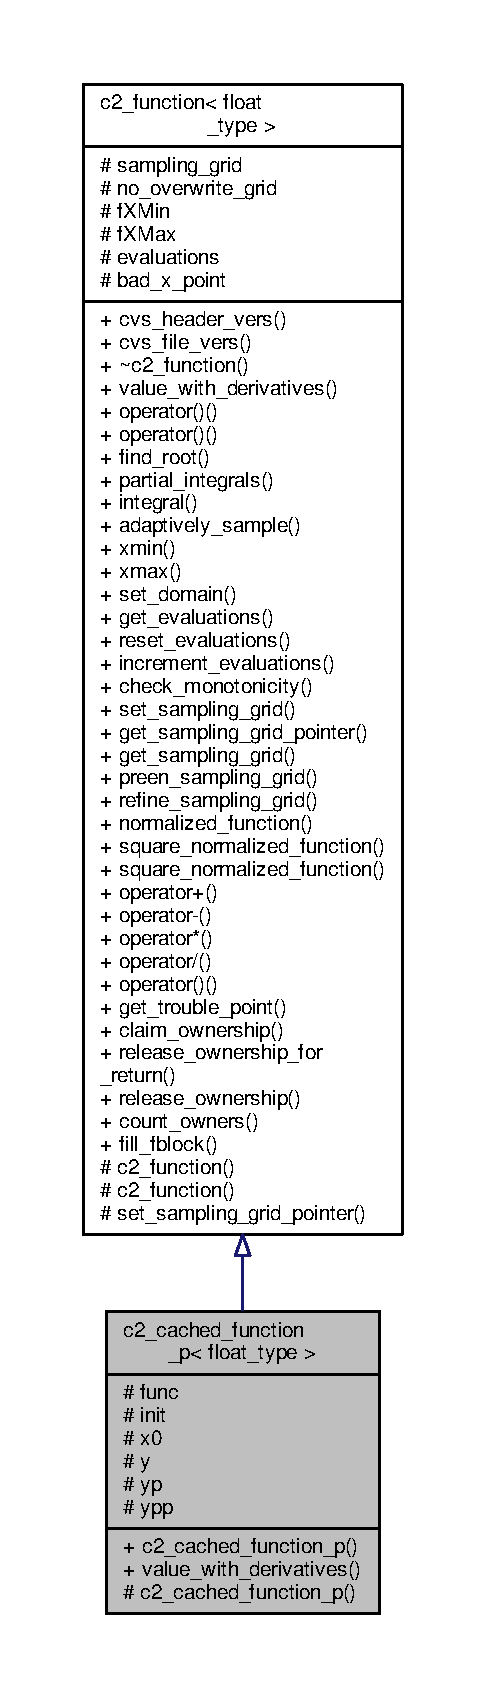
\includegraphics[height=550pt]{classc2__cached__function__p__inherit__graph}
\end{center}
\end{figure}


Collaboration diagram for c2\+\_\+cached\+\_\+function\+\_\+p$<$ float\+\_\+type $>$\+:
\nopagebreak
\begin{figure}[H]
\begin{center}
\leavevmode
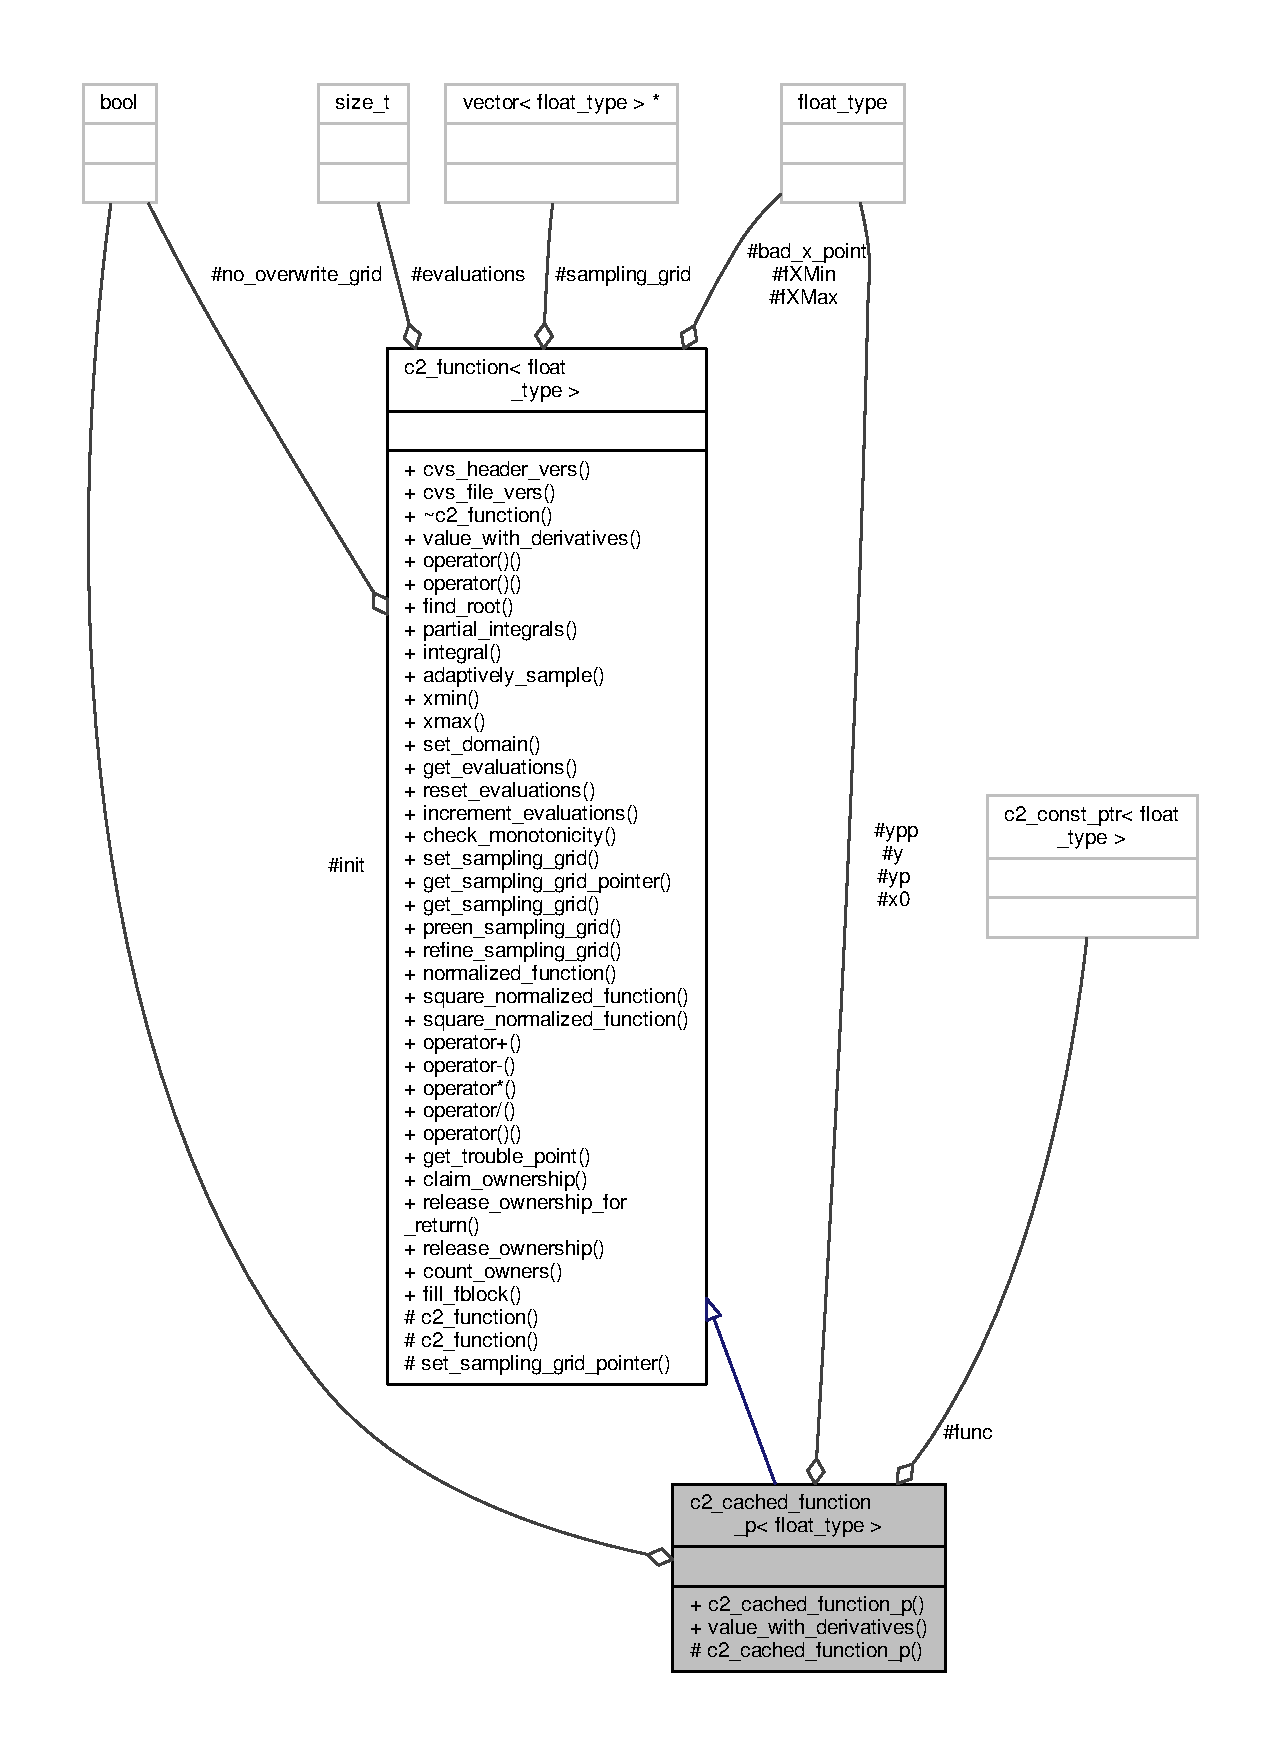
\includegraphics[width=350pt]{classc2__cached__function__p__coll__graph}
\end{center}
\end{figure}
\subsection*{Public Member Functions}
\begin{DoxyCompactItemize}
\item 
\hyperlink{classc2__cached__function__p_aac798ef75eb219dbf64a35fed575f217}{c2\+\_\+cached\+\_\+function\+\_\+p} (const \hyperlink{classc2__function}{c2\+\_\+function}$<$ float\+\_\+type $>$ \&f)
\begin{DoxyCompactList}\small\item\em construct the container \end{DoxyCompactList}\item 
virtual float\+\_\+type \hyperlink{classc2__cached__function__p_a09f22efcdcf81c1a7b353d10e29b193c}{value\+\_\+with\+\_\+derivatives} (float\+\_\+type x, float\+\_\+type $\ast$yprime, float\+\_\+type $\ast$yprime2) const   throw (c2\+\_\+exception)
\begin{DoxyCompactList}\small\item\em get the value and derivatives. \end{DoxyCompactList}\end{DoxyCompactItemize}
\subsection*{Protected Member Functions}
\begin{DoxyCompactItemize}
\item 
\hyperlink{classc2__cached__function__p_a0ab20552983f693a3a6eb1603858f21d}{c2\+\_\+cached\+\_\+function\+\_\+p} ()
\end{DoxyCompactItemize}
\subsection*{Protected Attributes}
\begin{DoxyCompactItemize}
\item 
const \hyperlink{classc2__const__ptr}{c2\+\_\+const\+\_\+ptr}$<$ float\+\_\+type $>$ \hyperlink{classc2__cached__function__p_a3918bce2ff2768a71256c5ef9346416e}{func}
\item 
bool \hyperlink{classc2__cached__function__p_a67f6484e64960b65ae0f7127d72707ff}{init}
\item 
float\+\_\+type \hyperlink{classc2__cached__function__p_a0dac26fccad111242068e3b43e387483}{x0}
\item 
float\+\_\+type \hyperlink{classc2__cached__function__p_a0104e340e54e7e0b7da2ac4ed5fce2a8}{y}
\item 
float\+\_\+type \hyperlink{classc2__cached__function__p_a5e6fa7f5df36abad202ae18c94555cf9}{yp}
\item 
float\+\_\+type \hyperlink{classc2__cached__function__p_aa4c8bb8e2184ba1560aa3c63cb73095a}{ypp}
\end{DoxyCompactItemize}


\subsection{Detailed Description}
\subsubsection*{template$<$typename float\+\_\+type = double$>$\\*
class c2\+\_\+cached\+\_\+function\+\_\+p$<$ float\+\_\+type $>$}

A container into which any other \hyperlink{classc2__function}{c2\+\_\+function} can be dropped.

It allows a function to be pre-\/evaluated at a point, and used at multiple places in an expression efficiently. If it is re-\/evaluated at the previous point, it returns the remembered values; otherwise, it re-\/evauates the function at the new point. 

The factory function \hyperlink{classc2__factory_aff889f94ad411d97f2e47f1c55fd0324}{c2\+\_\+factory\+::cached\+\_\+function()} creates $\ast$new \hyperlink{classc2__cached__function__p}{c2\+\_\+cached\+\_\+function\+\_\+p} 

\subsection{Constructor \& Destructor Documentation}
\index{c2\+\_\+cached\+\_\+function\+\_\+p@{c2\+\_\+cached\+\_\+function\+\_\+p}!c2\+\_\+cached\+\_\+function\+\_\+p@{c2\+\_\+cached\+\_\+function\+\_\+p}}
\index{c2\+\_\+cached\+\_\+function\+\_\+p@{c2\+\_\+cached\+\_\+function\+\_\+p}!c2\+\_\+cached\+\_\+function\+\_\+p@{c2\+\_\+cached\+\_\+function\+\_\+p}}
\subsubsection[{\texorpdfstring{c2\+\_\+cached\+\_\+function\+\_\+p(const c2\+\_\+function$<$ float\+\_\+type $>$ \&f)}{c2_cached_function_p(const c2_function< float_type > &f)}}]{\setlength{\rightskip}{0pt plus 5cm}template$<$typename float\+\_\+type  = double$>$ {\bf c2\+\_\+cached\+\_\+function\+\_\+p}$<$ float\+\_\+type $>$\+::{\bf c2\+\_\+cached\+\_\+function\+\_\+p} (
\begin{DoxyParamCaption}
\item[{const {\bf c2\+\_\+function}$<$ float\+\_\+type $>$ \&}]{f}
\end{DoxyParamCaption}
)\hspace{0.3cm}{\ttfamily [inline]}}\hypertarget{classc2__cached__function__p_aac798ef75eb219dbf64a35fed575f217}{}\label{classc2__cached__function__p_aac798ef75eb219dbf64a35fed575f217}


construct the container 


\begin{DoxyParams}{Parameters}
{\em f} & the function to be cached \\
\hline
\end{DoxyParams}
\index{c2\+\_\+cached\+\_\+function\+\_\+p@{c2\+\_\+cached\+\_\+function\+\_\+p}!c2\+\_\+cached\+\_\+function\+\_\+p@{c2\+\_\+cached\+\_\+function\+\_\+p}}
\index{c2\+\_\+cached\+\_\+function\+\_\+p@{c2\+\_\+cached\+\_\+function\+\_\+p}!c2\+\_\+cached\+\_\+function\+\_\+p@{c2\+\_\+cached\+\_\+function\+\_\+p}}
\subsubsection[{\texorpdfstring{c2\+\_\+cached\+\_\+function\+\_\+p()}{c2_cached_function_p()}}]{\setlength{\rightskip}{0pt plus 5cm}template$<$typename float\+\_\+type  = double$>$ {\bf c2\+\_\+cached\+\_\+function\+\_\+p}$<$ float\+\_\+type $>$\+::{\bf c2\+\_\+cached\+\_\+function\+\_\+p} (
\begin{DoxyParamCaption}
{}
\end{DoxyParamCaption}
)\hspace{0.3cm}{\ttfamily [inline]}, {\ttfamily [protected]}}\hypertarget{classc2__cached__function__p_a0ab20552983f693a3a6eb1603858f21d}{}\label{classc2__cached__function__p_a0ab20552983f693a3a6eb1603858f21d}


\subsection{Member Function Documentation}
\index{c2\+\_\+cached\+\_\+function\+\_\+p@{c2\+\_\+cached\+\_\+function\+\_\+p}!value\+\_\+with\+\_\+derivatives@{value\+\_\+with\+\_\+derivatives}}
\index{value\+\_\+with\+\_\+derivatives@{value\+\_\+with\+\_\+derivatives}!c2\+\_\+cached\+\_\+function\+\_\+p@{c2\+\_\+cached\+\_\+function\+\_\+p}}
\subsubsection[{\texorpdfstring{value\+\_\+with\+\_\+derivatives(float\+\_\+type x, float\+\_\+type $\ast$yprime, float\+\_\+type $\ast$yprime2) const }{value_with_derivatives(float_type x, float_type *yprime, float_type *yprime2) const }}]{\setlength{\rightskip}{0pt plus 5cm}template$<$typename float\+\_\+type  = double$>$ virtual float\+\_\+type {\bf c2\+\_\+cached\+\_\+function\+\_\+p}$<$ float\+\_\+type $>$\+::value\+\_\+with\+\_\+derivatives (
\begin{DoxyParamCaption}
\item[{float\+\_\+type}]{x, }
\item[{float\+\_\+type $\ast$}]{yprime, }
\item[{float\+\_\+type $\ast$}]{yprime2}
\end{DoxyParamCaption}
) const throw  {\bf c2\+\_\+exception}) \hspace{0.3cm}{\ttfamily [inline]}, {\ttfamily [virtual]}}\hypertarget{classc2__cached__function__p_a09f22efcdcf81c1a7b353d10e29b193c}{}\label{classc2__cached__function__p_a09f22efcdcf81c1a7b353d10e29b193c}


get the value and derivatives. 

There is required checking for null pointers on the derivatives, and most implementations should operate faster if derivatives are not needed. 
\begin{DoxyParams}[1]{Parameters}
\mbox{\tt in}  & {\em x} & the point at which to evaluate the function \\
\hline
\mbox{\tt out}  & {\em yprime} & the first derivative (if pointer is non-\/null) \\
\hline
\mbox{\tt out}  & {\em yprime2} & the second derivative (if pointer is non-\/null) \\
\hline
\end{DoxyParams}
\begin{DoxyReturn}{Returns}
the value of the function
\end{DoxyReturn}
Checks to see if the function is being re-\/evaluated at the previous point, and returns remembered values if so. 

Implements \hyperlink{classc2__function_a44e0201159111350be7f746fc9026f67}{c2\+\_\+function$<$ float\+\_\+type $>$}.



\subsection{Member Data Documentation}
\index{c2\+\_\+cached\+\_\+function\+\_\+p@{c2\+\_\+cached\+\_\+function\+\_\+p}!func@{func}}
\index{func@{func}!c2\+\_\+cached\+\_\+function\+\_\+p@{c2\+\_\+cached\+\_\+function\+\_\+p}}
\subsubsection[{\texorpdfstring{func}{func}}]{\setlength{\rightskip}{0pt plus 5cm}template$<$typename float\+\_\+type  = double$>$ const {\bf c2\+\_\+const\+\_\+ptr}$<$float\+\_\+type$>$ {\bf c2\+\_\+cached\+\_\+function\+\_\+p}$<$ float\+\_\+type $>$\+::func\hspace{0.3cm}{\ttfamily [protected]}}\hypertarget{classc2__cached__function__p_a3918bce2ff2768a71256c5ef9346416e}{}\label{classc2__cached__function__p_a3918bce2ff2768a71256c5ef9346416e}
\index{c2\+\_\+cached\+\_\+function\+\_\+p@{c2\+\_\+cached\+\_\+function\+\_\+p}!init@{init}}
\index{init@{init}!c2\+\_\+cached\+\_\+function\+\_\+p@{c2\+\_\+cached\+\_\+function\+\_\+p}}
\subsubsection[{\texorpdfstring{init}{init}}]{\setlength{\rightskip}{0pt plus 5cm}template$<$typename float\+\_\+type  = double$>$ bool {\bf c2\+\_\+cached\+\_\+function\+\_\+p}$<$ float\+\_\+type $>$\+::init\hspace{0.3cm}{\ttfamily [mutable]}, {\ttfamily [protected]}}\hypertarget{classc2__cached__function__p_a67f6484e64960b65ae0f7127d72707ff}{}\label{classc2__cached__function__p_a67f6484e64960b65ae0f7127d72707ff}
\index{c2\+\_\+cached\+\_\+function\+\_\+p@{c2\+\_\+cached\+\_\+function\+\_\+p}!x0@{x0}}
\index{x0@{x0}!c2\+\_\+cached\+\_\+function\+\_\+p@{c2\+\_\+cached\+\_\+function\+\_\+p}}
\subsubsection[{\texorpdfstring{x0}{x0}}]{\setlength{\rightskip}{0pt plus 5cm}template$<$typename float\+\_\+type  = double$>$ float\+\_\+type {\bf c2\+\_\+cached\+\_\+function\+\_\+p}$<$ float\+\_\+type $>$\+::x0\hspace{0.3cm}{\ttfamily [mutable]}, {\ttfamily [protected]}}\hypertarget{classc2__cached__function__p_a0dac26fccad111242068e3b43e387483}{}\label{classc2__cached__function__p_a0dac26fccad111242068e3b43e387483}
\index{c2\+\_\+cached\+\_\+function\+\_\+p@{c2\+\_\+cached\+\_\+function\+\_\+p}!y@{y}}
\index{y@{y}!c2\+\_\+cached\+\_\+function\+\_\+p@{c2\+\_\+cached\+\_\+function\+\_\+p}}
\subsubsection[{\texorpdfstring{y}{y}}]{\setlength{\rightskip}{0pt plus 5cm}template$<$typename float\+\_\+type  = double$>$ float\+\_\+type {\bf c2\+\_\+cached\+\_\+function\+\_\+p}$<$ float\+\_\+type $>$\+::y\hspace{0.3cm}{\ttfamily [mutable]}, {\ttfamily [protected]}}\hypertarget{classc2__cached__function__p_a0104e340e54e7e0b7da2ac4ed5fce2a8}{}\label{classc2__cached__function__p_a0104e340e54e7e0b7da2ac4ed5fce2a8}
\index{c2\+\_\+cached\+\_\+function\+\_\+p@{c2\+\_\+cached\+\_\+function\+\_\+p}!yp@{yp}}
\index{yp@{yp}!c2\+\_\+cached\+\_\+function\+\_\+p@{c2\+\_\+cached\+\_\+function\+\_\+p}}
\subsubsection[{\texorpdfstring{yp}{yp}}]{\setlength{\rightskip}{0pt plus 5cm}template$<$typename float\+\_\+type  = double$>$ float\+\_\+type {\bf c2\+\_\+cached\+\_\+function\+\_\+p}$<$ float\+\_\+type $>$\+::yp\hspace{0.3cm}{\ttfamily [mutable]}, {\ttfamily [protected]}}\hypertarget{classc2__cached__function__p_a5e6fa7f5df36abad202ae18c94555cf9}{}\label{classc2__cached__function__p_a5e6fa7f5df36abad202ae18c94555cf9}
\index{c2\+\_\+cached\+\_\+function\+\_\+p@{c2\+\_\+cached\+\_\+function\+\_\+p}!ypp@{ypp}}
\index{ypp@{ypp}!c2\+\_\+cached\+\_\+function\+\_\+p@{c2\+\_\+cached\+\_\+function\+\_\+p}}
\subsubsection[{\texorpdfstring{ypp}{ypp}}]{\setlength{\rightskip}{0pt plus 5cm}template$<$typename float\+\_\+type  = double$>$ float\+\_\+type {\bf c2\+\_\+cached\+\_\+function\+\_\+p}$<$ float\+\_\+type $>$\+::ypp\hspace{0.3cm}{\ttfamily [mutable]}, {\ttfamily [protected]}}\hypertarget{classc2__cached__function__p_aa4c8bb8e2184ba1560aa3c63cb73095a}{}\label{classc2__cached__function__p_aa4c8bb8e2184ba1560aa3c63cb73095a}


The documentation for this class was generated from the following file\+:\begin{DoxyCompactItemize}
\item 
\hyperlink{c2__function_8hh}{c2\+\_\+function.\+hh}\end{DoxyCompactItemize}

\hypertarget{classc2__classic__function__p}{\section{c2\-\_\-classic\-\_\-function\-\_\-p$<$ float\-\_\-type $>$ Class Template Reference}
\label{classc2__classic__function__p}\index{c2\-\_\-classic\-\_\-function\-\_\-p$<$ float\-\_\-type $>$@{c2\-\_\-classic\-\_\-function\-\_\-p$<$ float\-\_\-type $>$}}
}


a container into which any conventional c-\/style function can be dropped, to create a degenerate \hyperlink{classc2__function}{c2\-\_\-function} without derivatives. Mostly useful for sampling into interpolating functions. construct a reference to this with c2\-\_\-classic\-\_\-function()

The factory function \hyperlink{classc2__factory_ae5c9140b2bfcc6416682562b99479974}{c2\-\_\-factory\-::classic\-\_\-function()} creates $\ast$new \hyperlink{classc2__classic__function__p_a8b2d09d67a8835902fd6c684d5b183b7}{c2\-\_\-classic\-\_\-function\-\_\-p()}  




{\ttfamily \#include $<$c2\-\_\-function.\-hh$>$}

Inheritance diagram for c2\-\_\-classic\-\_\-function\-\_\-p$<$ float\-\_\-type $>$\-:\begin{figure}[H]
\begin{center}
\leavevmode
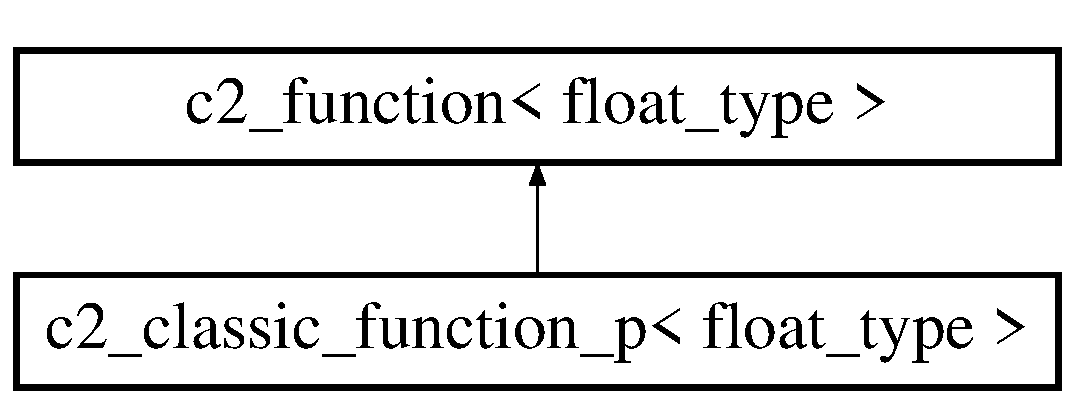
\includegraphics[height=2.000000cm]{classc2__classic__function__p}
\end{center}
\end{figure}
\subsection*{Public Member Functions}
\begin{DoxyCompactItemize}
\item 
\hyperlink{classc2__classic__function__p_a8b2d09d67a8835902fd6c684d5b183b7}{c2\-\_\-classic\-\_\-function\-\_\-p} (const float\-\_\-type($\ast$c\-\_\-func)(float\-\_\-type))
\begin{DoxyCompactList}\small\item\em construct the container \end{DoxyCompactList}\item 
virtual float\-\_\-type \hyperlink{classc2__classic__function__p_abf7fc11b0396fc249eb3300ed39b3cc3}{value\-\_\-with\-\_\-derivatives} (float\-\_\-type x, float\-\_\-type $\ast$yprime, float\-\_\-type $\ast$yprime2) const   throw (c2\-\_\-exception)
\begin{DoxyCompactList}\small\item\em get the value and derivatives. \end{DoxyCompactList}\end{DoxyCompactItemize}
\subsection*{Protected Attributes}
\begin{DoxyCompactItemize}
\item 
\hypertarget{classc2__classic__function__p_a1ff2ac38a9a119e6f68ef44bb382ece7}{const float\-\_\-type($\ast$ \hyperlink{classc2__classic__function__p_a1ff2ac38a9a119e6f68ef44bb382ece7}{func} )(float\-\_\-type)}\label{classc2__classic__function__p_a1ff2ac38a9a119e6f68ef44bb382ece7}

\begin{DoxyCompactList}\small\item\em pointer to our function \end{DoxyCompactList}\end{DoxyCompactItemize}
\subsection*{Additional Inherited Members}


\subsection{Detailed Description}
\subsubsection*{template$<$typename float\-\_\-type = double$>$class c2\-\_\-classic\-\_\-function\-\_\-p$<$ float\-\_\-type $>$}

a container into which any conventional c-\/style function can be dropped, to create a degenerate \hyperlink{classc2__function}{c2\-\_\-function} without derivatives. Mostly useful for sampling into interpolating functions. construct a reference to this with c2\-\_\-classic\-\_\-function()

The factory function \hyperlink{classc2__factory_ae5c9140b2bfcc6416682562b99479974}{c2\-\_\-factory\-::classic\-\_\-function()} creates $\ast$new \hyperlink{classc2__classic__function__p_a8b2d09d67a8835902fd6c684d5b183b7}{c2\-\_\-classic\-\_\-function\-\_\-p()} 

\subsection{Constructor \& Destructor Documentation}
\hypertarget{classc2__classic__function__p_a8b2d09d67a8835902fd6c684d5b183b7}{\index{c2\-\_\-classic\-\_\-function\-\_\-p@{c2\-\_\-classic\-\_\-function\-\_\-p}!c2\-\_\-classic\-\_\-function\-\_\-p@{c2\-\_\-classic\-\_\-function\-\_\-p}}
\index{c2\-\_\-classic\-\_\-function\-\_\-p@{c2\-\_\-classic\-\_\-function\-\_\-p}!c2_classic_function_p@{c2\-\_\-classic\-\_\-function\-\_\-p}}
\subsubsection[{c2\-\_\-classic\-\_\-function\-\_\-p}]{\setlength{\rightskip}{0pt plus 5cm}template$<$typename float\-\_\-type  = double$>$ {\bf c2\-\_\-classic\-\_\-function\-\_\-p}$<$ float\-\_\-type $>$\-::{\bf c2\-\_\-classic\-\_\-function\-\_\-p} (
\begin{DoxyParamCaption}
\item[{const float\-\_\-type($\ast$)(float\-\_\-type)}]{c\-\_\-func}
\end{DoxyParamCaption}
)\hspace{0.3cm}{\ttfamily [inline]}}}\label{classc2__classic__function__p_a8b2d09d67a8835902fd6c684d5b183b7}


construct the container 


\begin{DoxyParams}{Parameters}
{\em c\-\_\-func} & a pointer to a conventional c-\/style function \\
\hline
\end{DoxyParams}


\subsection{Member Function Documentation}
\hypertarget{classc2__classic__function__p_abf7fc11b0396fc249eb3300ed39b3cc3}{\index{c2\-\_\-classic\-\_\-function\-\_\-p@{c2\-\_\-classic\-\_\-function\-\_\-p}!value\-\_\-with\-\_\-derivatives@{value\-\_\-with\-\_\-derivatives}}
\index{value\-\_\-with\-\_\-derivatives@{value\-\_\-with\-\_\-derivatives}!c2_classic_function_p@{c2\-\_\-classic\-\_\-function\-\_\-p}}
\subsubsection[{value\-\_\-with\-\_\-derivatives}]{\setlength{\rightskip}{0pt plus 5cm}template$<$typename float\-\_\-type  = double$>$ virtual float\-\_\-type {\bf c2\-\_\-classic\-\_\-function\-\_\-p}$<$ float\-\_\-type $>$\-::value\-\_\-with\-\_\-derivatives (
\begin{DoxyParamCaption}
\item[{float\-\_\-type}]{x, }
\item[{float\-\_\-type $\ast$}]{yprime, }
\item[{float\-\_\-type $\ast$}]{yprime2}
\end{DoxyParamCaption}
) const throw  {\bf c2\-\_\-exception}) \hspace{0.3cm}{\ttfamily [inline]}, {\ttfamily [virtual]}}}\label{classc2__classic__function__p_abf7fc11b0396fc249eb3300ed39b3cc3}


get the value and derivatives. 

There is required checking for null pointers on the derivatives, and most implementations should operate faster if derivatives are not needed. 
\begin{DoxyParams}[1]{Parameters}
\mbox{\tt in}  & {\em x} & the point at which to evaluate the function \\
\hline
\mbox{\tt out}  & {\em yprime} & the first derivative (if pointer is non-\/null) \\
\hline
\mbox{\tt out}  & {\em yprime2} & the second derivative (if pointer is non-\/null) \\
\hline
\end{DoxyParams}
\begin{DoxyReturn}{Returns}
the value of the function Uses the internal function pointer set by set\-\_\-function(). 
\end{DoxyReturn}


Implements \hyperlink{classc2__function_a44e0201159111350be7f746fc9026f67}{c2\-\_\-function$<$ float\-\_\-type $>$}.



The documentation for this class was generated from the following file\-:\begin{DoxyCompactItemize}
\item 
\hyperlink{c2__function_8hh}{c2\-\_\-function.\-hh}\end{DoxyCompactItemize}

\hypertarget{classc2__composed__function__p}{}\section{c2\+\_\+composed\+\_\+function\+\_\+p$<$ float\+\_\+type $>$ Class Template Reference}
\label{classc2__composed__function__p}\index{c2\+\_\+composed\+\_\+function\+\_\+p$<$ float\+\_\+type $>$@{c2\+\_\+composed\+\_\+function\+\_\+p$<$ float\+\_\+type $>$}}


Provides function composition (nesting)

This allows evaluation of {\itshape f(g(x))} where {\itshape f} and {\itshape g} are \hyperlink{classc2__function}{c2\+\_\+function} objects.  




{\ttfamily \#include \char`\"{}c2\+\_\+function.\+hh\char`\"{}}



Inheritance diagram for c2\+\_\+composed\+\_\+function\+\_\+p$<$ float\+\_\+type $>$\+:
\nopagebreak
\begin{figure}[H]
\begin{center}
\leavevmode
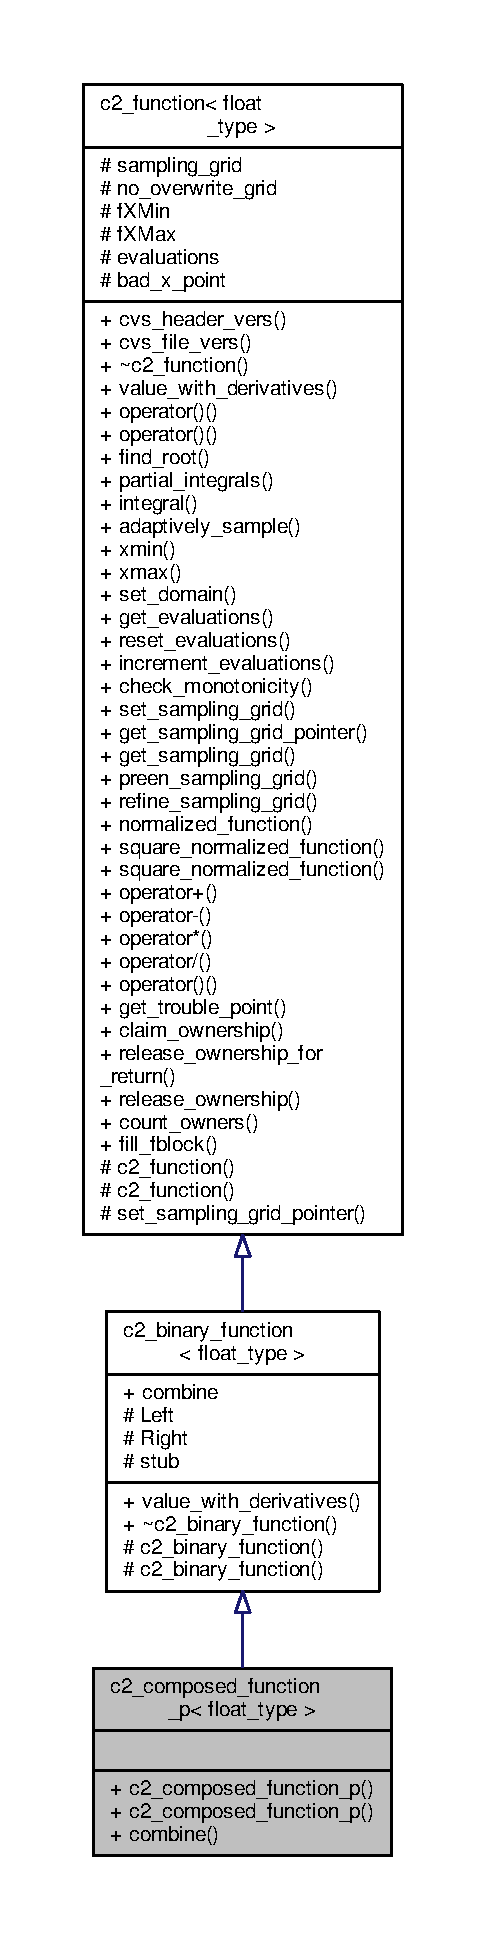
\includegraphics[height=550pt]{classc2__composed__function__p__inherit__graph}
\end{center}
\end{figure}


Collaboration diagram for c2\+\_\+composed\+\_\+function\+\_\+p$<$ float\+\_\+type $>$\+:
\nopagebreak
\begin{figure}[H]
\begin{center}
\leavevmode
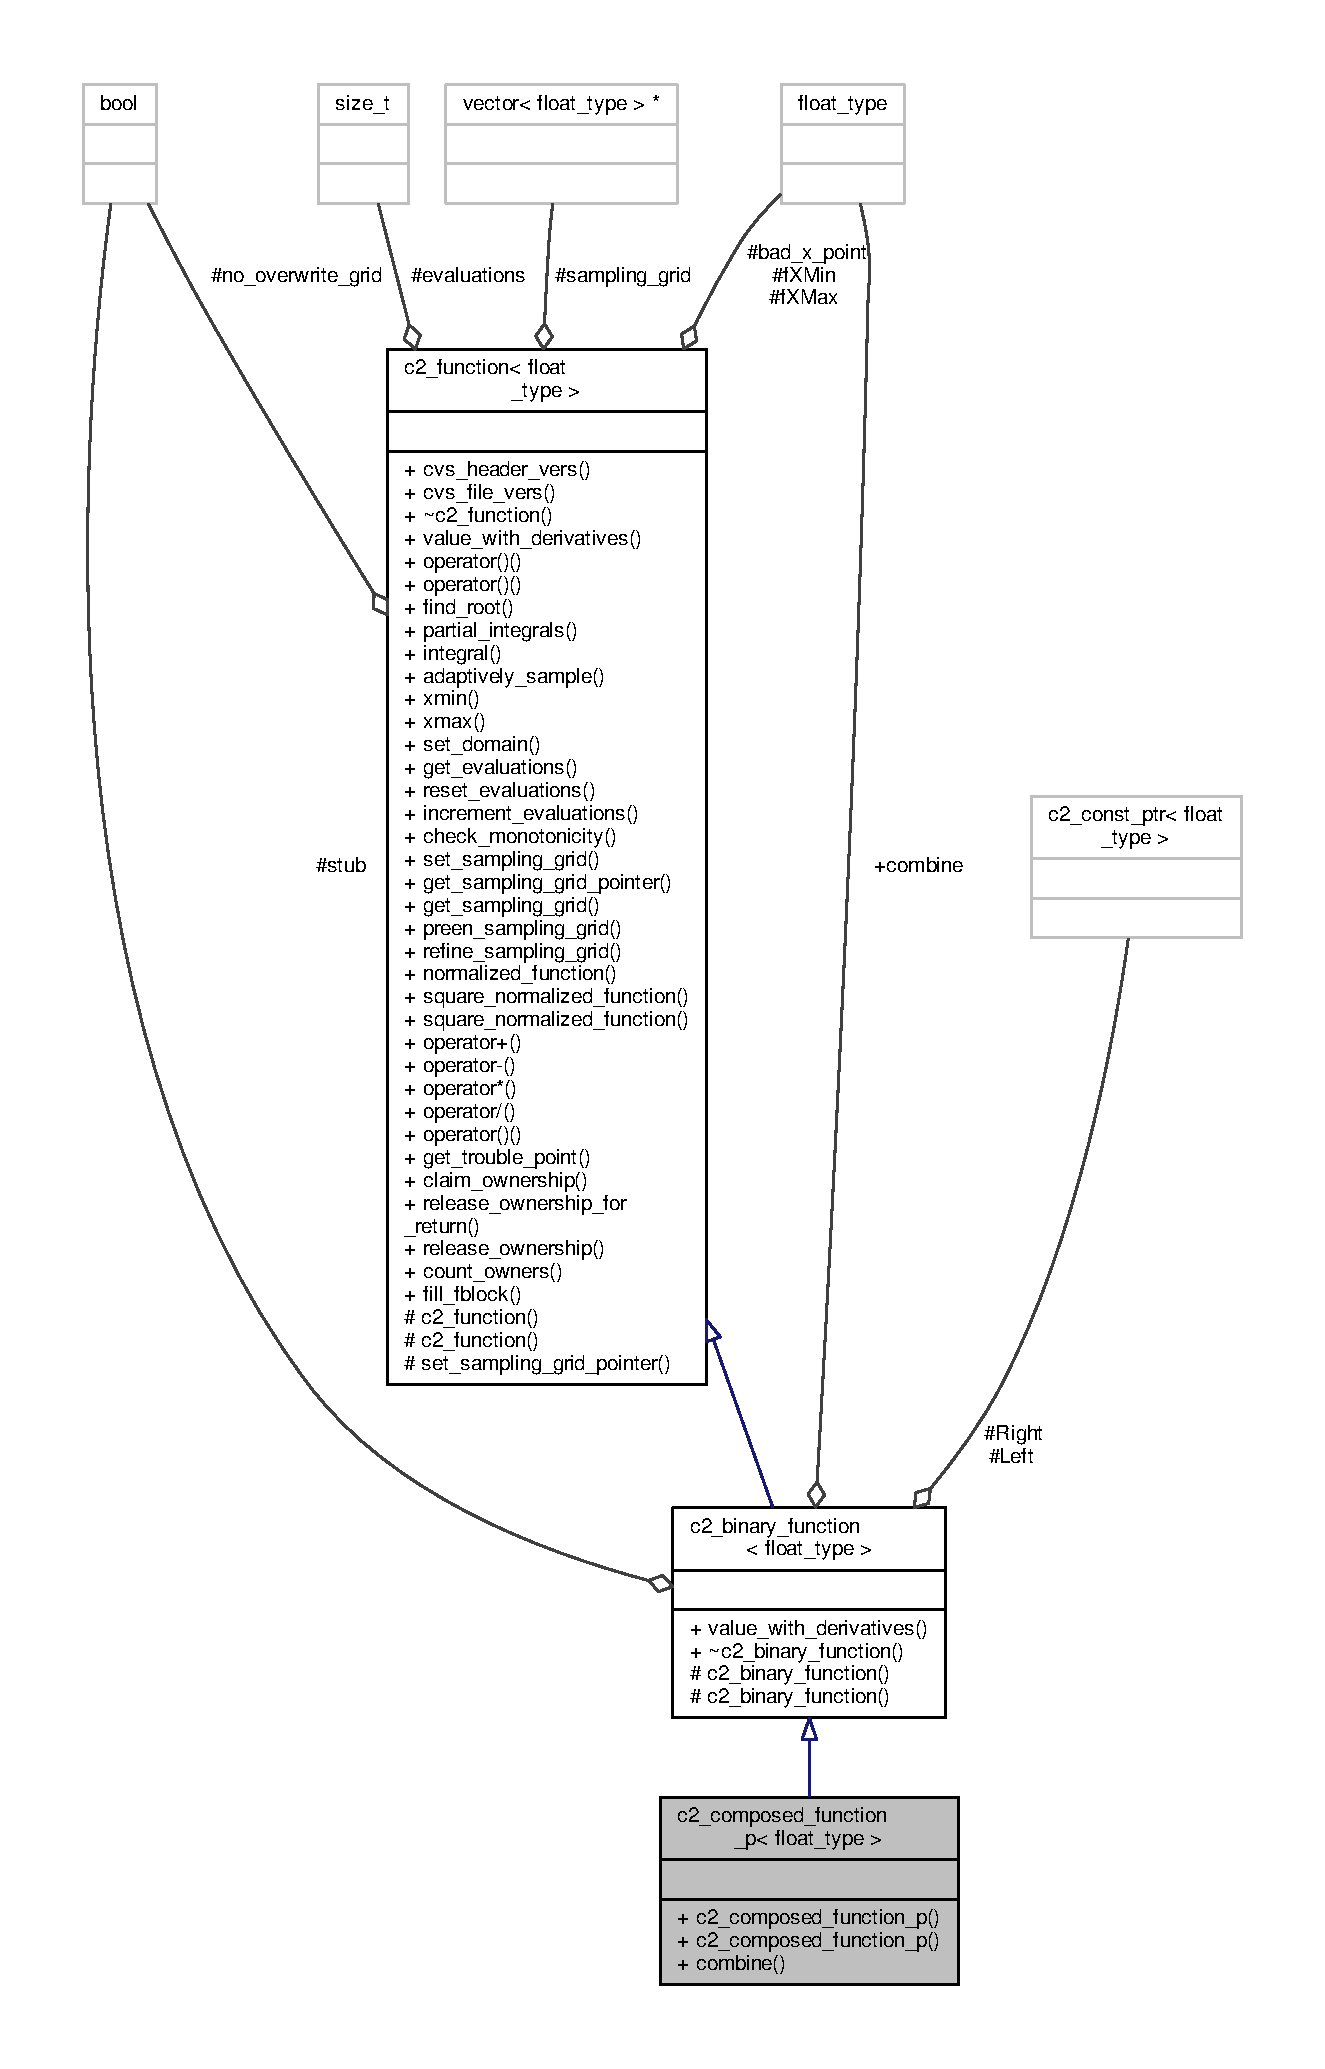
\includegraphics[width=350pt]{classc2__composed__function__p__coll__graph}
\end{center}
\end{figure}
\subsection*{Public Member Functions}
\begin{DoxyCompactItemize}
\item 
\hyperlink{classc2__composed__function__p_a45b7f7de47d2c363d51aa4f953e85edf}{c2\+\_\+composed\+\_\+function\+\_\+p} (const \hyperlink{classc2__function}{c2\+\_\+function}$<$ float\+\_\+type $>$ \&outer, const \hyperlink{classc2__function}{c2\+\_\+function}$<$ float\+\_\+type $>$ \&inner)
\begin{DoxyCompactList}\small\item\em construct {\itshape outer}( {\itshape inner} (x)) \end{DoxyCompactList}\item 
\hyperlink{classc2__composed__function__p_a5a1db2d4db6b02e054034452be85be06}{c2\+\_\+composed\+\_\+function\+\_\+p} ()
\begin{DoxyCompactList}\small\item\em Create a stub just for the combiner to avoid statics. \end{DoxyCompactList}\end{DoxyCompactItemize}
\subsection*{Static Public Member Functions}
\begin{DoxyCompactItemize}
\item 
static float\+\_\+type \hyperlink{classc2__composed__function__p_a9431a8977df47ca1fde4a4ba92525781}{combine} (const \hyperlink{classc2__function}{c2\+\_\+function}$<$ float\+\_\+type $>$ \&left, const \hyperlink{classc2__function}{c2\+\_\+function}$<$ float\+\_\+type $>$ \&right, float\+\_\+type x, float\+\_\+type $\ast$yprime, float\+\_\+type $\ast$yprime2)  throw (c2\+\_\+exception)
\begin{DoxyCompactList}\small\item\em execute math necessary to do composition \end{DoxyCompactList}\end{DoxyCompactItemize}
\subsection*{Additional Inherited Members}


\subsection{Detailed Description}
\subsubsection*{template$<$typename float\+\_\+type = double$>$\\*
class c2\+\_\+composed\+\_\+function\+\_\+p$<$ float\+\_\+type $>$}

Provides function composition (nesting)

This allows evaluation of {\itshape f(g(x))} where {\itshape f} and {\itshape g} are \hyperlink{classc2__function}{c2\+\_\+function} objects. 

This should always be constructed using \hyperlink{classc2__function_compose_operator}{c2\+\_\+function\+:\+:operator()} 

\subsection{Constructor \& Destructor Documentation}
\index{c2\+\_\+composed\+\_\+function\+\_\+p@{c2\+\_\+composed\+\_\+function\+\_\+p}!c2\+\_\+composed\+\_\+function\+\_\+p@{c2\+\_\+composed\+\_\+function\+\_\+p}}
\index{c2\+\_\+composed\+\_\+function\+\_\+p@{c2\+\_\+composed\+\_\+function\+\_\+p}!c2\+\_\+composed\+\_\+function\+\_\+p@{c2\+\_\+composed\+\_\+function\+\_\+p}}
\subsubsection[{\texorpdfstring{c2\+\_\+composed\+\_\+function\+\_\+p(const c2\+\_\+function$<$ float\+\_\+type $>$ \&outer, const c2\+\_\+function$<$ float\+\_\+type $>$ \&inner)}{c2_composed_function_p(const c2_function< float_type > &outer, const c2_function< float_type > &inner)}}]{\setlength{\rightskip}{0pt plus 5cm}template$<$typename float\+\_\+type = double$>$ {\bf c2\+\_\+composed\+\_\+function\+\_\+p}$<$ float\+\_\+type $>$\+::{\bf c2\+\_\+composed\+\_\+function\+\_\+p} (
\begin{DoxyParamCaption}
\item[{const {\bf c2\+\_\+function}$<$ float\+\_\+type $>$ \&}]{outer, }
\item[{const {\bf c2\+\_\+function}$<$ float\+\_\+type $>$ \&}]{inner}
\end{DoxyParamCaption}
)\hspace{0.3cm}{\ttfamily [inline]}}\hypertarget{classc2__composed__function__p_a45b7f7de47d2c363d51aa4f953e85edf}{}\label{classc2__composed__function__p_a45b7f7de47d2c363d51aa4f953e85edf}


construct {\itshape outer}( {\itshape inner} (x)) 

\begin{DoxyNote}{Note}
See \hyperlink{classc2__binary__function}{c2\+\_\+binary\+\_\+function} for discussion of ownership. 
\end{DoxyNote}

\begin{DoxyParams}{Parameters}
{\em outer} & the outer function \\
\hline
{\em inner} & the inner function \\
\hline
\end{DoxyParams}
\index{c2\+\_\+composed\+\_\+function\+\_\+p@{c2\+\_\+composed\+\_\+function\+\_\+p}!c2\+\_\+composed\+\_\+function\+\_\+p@{c2\+\_\+composed\+\_\+function\+\_\+p}}
\index{c2\+\_\+composed\+\_\+function\+\_\+p@{c2\+\_\+composed\+\_\+function\+\_\+p}!c2\+\_\+composed\+\_\+function\+\_\+p@{c2\+\_\+composed\+\_\+function\+\_\+p}}
\subsubsection[{\texorpdfstring{c2\+\_\+composed\+\_\+function\+\_\+p()}{c2_composed_function_p()}}]{\setlength{\rightskip}{0pt plus 5cm}template$<$typename float\+\_\+type = double$>$ {\bf c2\+\_\+composed\+\_\+function\+\_\+p}$<$ float\+\_\+type $>$\+::{\bf c2\+\_\+composed\+\_\+function\+\_\+p} (
\begin{DoxyParamCaption}
{}
\end{DoxyParamCaption}
)\hspace{0.3cm}{\ttfamily [inline]}}\hypertarget{classc2__composed__function__p_a5a1db2d4db6b02e054034452be85be06}{}\label{classc2__composed__function__p_a5a1db2d4db6b02e054034452be85be06}


Create a stub just for the combiner to avoid statics. 



\subsection{Member Function Documentation}
\index{c2\+\_\+composed\+\_\+function\+\_\+p@{c2\+\_\+composed\+\_\+function\+\_\+p}!combine@{combine}}
\index{combine@{combine}!c2\+\_\+composed\+\_\+function\+\_\+p@{c2\+\_\+composed\+\_\+function\+\_\+p}}
\subsubsection[{\texorpdfstring{combine(const c2\+\_\+function$<$ float\+\_\+type $>$ \&left, const c2\+\_\+function$<$ float\+\_\+type $>$ \&right, float\+\_\+type x, float\+\_\+type $\ast$yprime, float\+\_\+type $\ast$yprime2)}{combine(const c2_function< float_type > &left, const c2_function< float_type > &right, float_type x, float_type *yprime, float_type *yprime2)}}]{\setlength{\rightskip}{0pt plus 5cm}template$<$typename float\+\_\+type = double$>$ static float\+\_\+type {\bf c2\+\_\+composed\+\_\+function\+\_\+p}$<$ float\+\_\+type $>$\+::combine (
\begin{DoxyParamCaption}
\item[{const {\bf c2\+\_\+function}$<$ float\+\_\+type $>$ \&}]{left, }
\item[{const {\bf c2\+\_\+function}$<$ float\+\_\+type $>$ \&}]{right, }
\item[{float\+\_\+type}]{x, }
\item[{float\+\_\+type $\ast$}]{yprime, }
\item[{float\+\_\+type $\ast$}]{yprime2}
\end{DoxyParamCaption}
) throw  {\bf c2\+\_\+exception}) \hspace{0.3cm}{\ttfamily [inline]}, {\ttfamily [static]}}\hypertarget{classc2__composed__function__p_a9431a8977df47ca1fde4a4ba92525781}{}\label{classc2__composed__function__p_a9431a8977df47ca1fde4a4ba92525781}


execute math necessary to do composition 



The documentation for this class was generated from the following file\+:\begin{DoxyCompactItemize}
\item 
\hyperlink{c2__function_8hh}{c2\+\_\+function.\+hh}\end{DoxyCompactItemize}

\hypertarget{classc2__connector__function__p}{\section{c2\-\_\-connector\-\_\-function\-\_\-p$<$ float\-\_\-type $>$ Class Template Reference}
\label{classc2__connector__function__p}\index{c2\-\_\-connector\-\_\-function\-\_\-p$<$ float\-\_\-type $>$@{c2\-\_\-connector\-\_\-function\-\_\-p$<$ float\-\_\-type $>$}}
}


create a \hyperlink{classc2__function}{c2\-\_\-function} which smoothly connects two other c2\-\_\-functions.

This takes two points and generates a polynomial which matches two \hyperlink{classc2__function}{c2\-\_\-function} arguments at those two points, with two derivatives at each point, and an arbitrary value at the center of the region. It is useful for splicing together functions over rough spots (0/0, for example).  




{\ttfamily \#include $<$c2\-\_\-function.\-hh$>$}

Inheritance diagram for c2\-\_\-connector\-\_\-function\-\_\-p$<$ float\-\_\-type $>$\-:\begin{figure}[H]
\begin{center}
\leavevmode
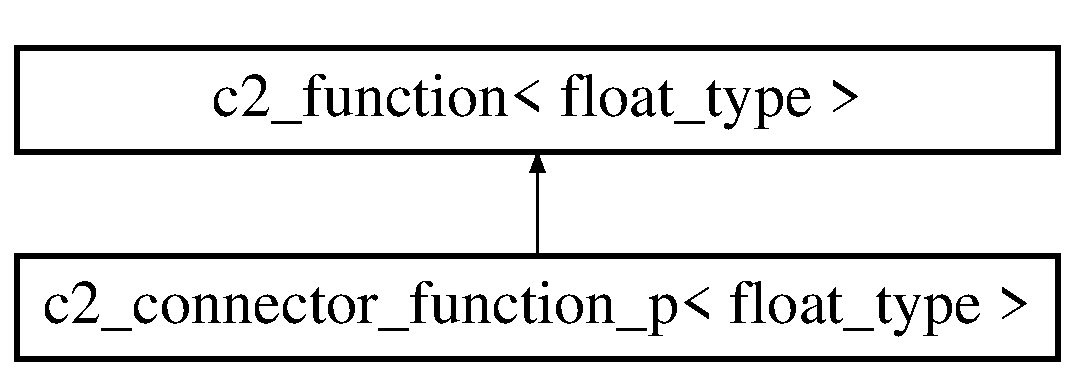
\includegraphics[height=2.000000cm]{classc2__connector__function__p}
\end{center}
\end{figure}
\subsection*{Public Member Functions}
\begin{DoxyCompactItemize}
\item 
\hyperlink{classc2__connector__function__p_a7827c6d4a19b57d2c63ac384cb91211c}{c2\-\_\-connector\-\_\-function\-\_\-p} (float\-\_\-type x0, const \hyperlink{classc2__function}{c2\-\_\-function}$<$ float\-\_\-type $>$ \&f0, float\-\_\-type x2, const \hyperlink{classc2__function}{c2\-\_\-function}$<$ float\-\_\-type $>$ \&f2, bool auto\-\_\-center, float\-\_\-type y1)
\begin{DoxyCompactList}\small\item\em construct the container from two functions \end{DoxyCompactList}\item 
\hyperlink{classc2__connector__function__p_a2445b30d02a6a968b0c36d39feefc537}{c2\-\_\-connector\-\_\-function\-\_\-p} (float\-\_\-type x0, float\-\_\-type y0, float\-\_\-type yp0, float\-\_\-type ypp0, float\-\_\-type x2, float\-\_\-type y2, float\-\_\-type yp2, float\-\_\-type ypp2, bool auto\-\_\-center, float\-\_\-type y1)
\begin{DoxyCompactList}\small\item\em construct the container from numerical values \end{DoxyCompactList}\item 
\hyperlink{classc2__connector__function__p_a359df91e0d5560c772cea46b22d7181c}{c2\-\_\-connector\-\_\-function\-\_\-p} (const \hyperlink{classc2__fblock}{c2\-\_\-fblock}$<$ float\-\_\-type $>$ \&fb0, const \hyperlink{classc2__fblock}{c2\-\_\-fblock}$<$ float\-\_\-type $>$ \&fb2, bool auto\-\_\-center, float\-\_\-type y1)
\begin{DoxyCompactList}\small\item\em construct the container from c2\-\_\-fblock$<$float\-\_\-type$>$ objects \end{DoxyCompactList}\item 
\hypertarget{classc2__connector__function__p_a3cf5737490d0653f6421cb8ea8390cbf}{virtual \hyperlink{classc2__connector__function__p_a3cf5737490d0653f6421cb8ea8390cbf}{$\sim$c2\-\_\-connector\-\_\-function\-\_\-p} ()}\label{classc2__connector__function__p_a3cf5737490d0653f6421cb8ea8390cbf}

\begin{DoxyCompactList}\small\item\em destructor \end{DoxyCompactList}\item 
virtual float\-\_\-type \hyperlink{classc2__connector__function__p_a0c748860e1ef547a0cce583c01abe175}{value\-\_\-with\-\_\-derivatives} (float\-\_\-type x, float\-\_\-type $\ast$yprime, float\-\_\-type $\ast$yprime2) const   throw (c2\-\_\-exception)
\begin{DoxyCompactList}\small\item\em get the value and derivatives. \end{DoxyCompactList}\end{DoxyCompactItemize}
\subsection*{Protected Member Functions}
\begin{DoxyCompactItemize}
\item 
\hypertarget{classc2__connector__function__p_af5f4cfcfcaf990a779710f25dedfff9b}{void \hyperlink{classc2__connector__function__p_af5f4cfcfcaf990a779710f25dedfff9b}{init} (const \hyperlink{classc2__fblock}{c2\-\_\-fblock}$<$ float\-\_\-type $>$ \&fb0, const \hyperlink{classc2__fblock}{c2\-\_\-fblock}$<$ float\-\_\-type $>$ \&fb2, bool auto\-\_\-center, float\-\_\-type y1)}\label{classc2__connector__function__p_af5f4cfcfcaf990a779710f25dedfff9b}

\begin{DoxyCompactList}\small\item\em fill container numerically \end{DoxyCompactList}\end{DoxyCompactItemize}
\subsection*{Protected Attributes}
\begin{DoxyCompactItemize}
\item 
\hypertarget{classc2__connector__function__p_aa9bafcf757d0607f897ab5e7d0acfb72}{float\-\_\-type {\bfseries fhinv}}\label{classc2__connector__function__p_aa9bafcf757d0607f897ab5e7d0acfb72}

\item 
\hypertarget{classc2__connector__function__p_a1e6f14a7d716a5915adf1985bbdc4c52}{float\-\_\-type {\bfseries fy1}}\label{classc2__connector__function__p_a1e6f14a7d716a5915adf1985bbdc4c52}

\item 
\hypertarget{classc2__connector__function__p_a3057f77c22dc61e93a1a3485780dd93f}{float\-\_\-type {\bfseries fa}}\label{classc2__connector__function__p_a3057f77c22dc61e93a1a3485780dd93f}

\item 
\hypertarget{classc2__connector__function__p_a3eff36726d4717fca41848605cd53916}{float\-\_\-type {\bfseries fb}}\label{classc2__connector__function__p_a3eff36726d4717fca41848605cd53916}

\item 
\hypertarget{classc2__connector__function__p_a0f0edb256a18551e2d054e47487d5b1d}{float\-\_\-type {\bfseries fc}}\label{classc2__connector__function__p_a0f0edb256a18551e2d054e47487d5b1d}

\item 
\hypertarget{classc2__connector__function__p_a2d06e77813b110a2c6ce09399d246704}{float\-\_\-type {\bfseries fd}}\label{classc2__connector__function__p_a2d06e77813b110a2c6ce09399d246704}

\item 
\hypertarget{classc2__connector__function__p_a64b954176b723477abf827e67bcfb7e7}{float\-\_\-type {\bfseries fe}}\label{classc2__connector__function__p_a64b954176b723477abf827e67bcfb7e7}

\item 
\hypertarget{classc2__connector__function__p_a39ca7caba5b003e6684eaf6c80920a8a}{float\-\_\-type {\bfseries ff}}\label{classc2__connector__function__p_a39ca7caba5b003e6684eaf6c80920a8a}

\end{DoxyCompactItemize}


\subsection{Detailed Description}
\subsubsection*{template$<$typename float\-\_\-type = double$>$class c2\-\_\-connector\-\_\-function\-\_\-p$<$ float\-\_\-type $>$}

create a \hyperlink{classc2__function}{c2\-\_\-function} which smoothly connects two other c2\-\_\-functions.

This takes two points and generates a polynomial which matches two \hyperlink{classc2__function}{c2\-\_\-function} arguments at those two points, with two derivatives at each point, and an arbitrary value at the center of the region. It is useful for splicing together functions over rough spots (0/0, for example). 

If {\itshape auto\-\_\-center} is true, the value at the midpoint is computed so that the resulting polynomial is of order 5. If {\itshape auto\-\_\-center} is false, the value {\itshape y1} is used at the midpoint, resulting in a polynomial of order 6.

This is usually used in conjunction with \hyperlink{classc2__piecewise__function__p}{c2\-\_\-piecewise\-\_\-function\-\_\-p} to assemble an apparently seamless function from a series of segments. \begin{DoxySeeAlso}{See Also}
Sample Applications and \hyperlink{classc2__function_aea75f73d6a97087571c163ae4e514652}{Adaptive sampling}
\end{DoxySeeAlso}
The factory function \hyperlink{classc2__factory_ac8c9d70e5c486a0025e288e5911f2a55}{c2\-\_\-factory\-::connector\-\_\-function()} creates $\ast$new \hyperlink{classc2__connector__function__p}{c2\-\_\-connector\-\_\-function\-\_\-p} 

\subsection{Constructor \& Destructor Documentation}
\hypertarget{classc2__connector__function__p_a7827c6d4a19b57d2c63ac384cb91211c}{\index{c2\-\_\-connector\-\_\-function\-\_\-p@{c2\-\_\-connector\-\_\-function\-\_\-p}!c2\-\_\-connector\-\_\-function\-\_\-p@{c2\-\_\-connector\-\_\-function\-\_\-p}}
\index{c2\-\_\-connector\-\_\-function\-\_\-p@{c2\-\_\-connector\-\_\-function\-\_\-p}!c2_connector_function_p@{c2\-\_\-connector\-\_\-function\-\_\-p}}
\subsubsection[{c2\-\_\-connector\-\_\-function\-\_\-p}]{\setlength{\rightskip}{0pt plus 5cm}template$<$typename float\-\_\-type = double$>$ {\bf c2\-\_\-connector\-\_\-function\-\_\-p}$<$ float\-\_\-type $>$\-::{\bf c2\-\_\-connector\-\_\-function\-\_\-p} (
\begin{DoxyParamCaption}
\item[{float\-\_\-type}]{x0, }
\item[{const {\bf c2\-\_\-function}$<$ float\-\_\-type $>$ \&}]{f0, }
\item[{float\-\_\-type}]{x2, }
\item[{const {\bf c2\-\_\-function}$<$ float\-\_\-type $>$ \&}]{f2, }
\item[{bool}]{auto\-\_\-center, }
\item[{float\-\_\-type}]{y1}
\end{DoxyParamCaption}
)}}\label{classc2__connector__function__p_a7827c6d4a19b57d2c63ac384cb91211c}


construct the container from two functions 


\begin{DoxyParams}{Parameters}
{\em x0} & the point at which to match {\itshape f1} and its derivatives \\
\hline
{\em f0} & the function on the left side to be connected \\
\hline
{\em x2} & the point at which to match {\itshape f2} and its derivatives \\
\hline
{\em f2} & the function on the right side to be connected \\
\hline
{\em auto\-\_\-center} & if true, no midpoint value is specified. If false, match the value {\itshape y1} at the midpoint \\
\hline
{\em y1} & the value to match at the midpoint, if {\itshape auto\-\_\-center} is false \\
\hline
\end{DoxyParams}
\begin{DoxyReturn}{Returns}
a \hyperlink{classc2__function}{c2\-\_\-function} with domain ({\itshape x0},{\itshape x2}) which smoothly connects {\itshape f0(x0)} and {\itshape f2(x2)} 
\end{DoxyReturn}
\hypertarget{classc2__connector__function__p_a2445b30d02a6a968b0c36d39feefc537}{\index{c2\-\_\-connector\-\_\-function\-\_\-p@{c2\-\_\-connector\-\_\-function\-\_\-p}!c2\-\_\-connector\-\_\-function\-\_\-p@{c2\-\_\-connector\-\_\-function\-\_\-p}}
\index{c2\-\_\-connector\-\_\-function\-\_\-p@{c2\-\_\-connector\-\_\-function\-\_\-p}!c2_connector_function_p@{c2\-\_\-connector\-\_\-function\-\_\-p}}
\subsubsection[{c2\-\_\-connector\-\_\-function\-\_\-p}]{\setlength{\rightskip}{0pt plus 5cm}template$<$typename float\-\_\-type = double$>$ {\bf c2\-\_\-connector\-\_\-function\-\_\-p}$<$ float\-\_\-type $>$\-::{\bf c2\-\_\-connector\-\_\-function\-\_\-p} (
\begin{DoxyParamCaption}
\item[{float\-\_\-type}]{x0, }
\item[{float\-\_\-type}]{y0, }
\item[{float\-\_\-type}]{yp0, }
\item[{float\-\_\-type}]{ypp0, }
\item[{float\-\_\-type}]{x2, }
\item[{float\-\_\-type}]{y2, }
\item[{float\-\_\-type}]{yp2, }
\item[{float\-\_\-type}]{ypp2, }
\item[{bool}]{auto\-\_\-center, }
\item[{float\-\_\-type}]{y1}
\end{DoxyParamCaption}
)}}\label{classc2__connector__function__p_a2445b30d02a6a968b0c36d39feefc537}


construct the container from numerical values 


\begin{DoxyParams}{Parameters}
{\em x0} & the position of the left edge \\
\hline
{\em y0} & the function derivative on the left boundary \\
\hline
{\em yp0} & the function second derivative on the left boundary \\
\hline
{\em ypp0} & the function value on the left boundary \\
\hline
{\em x2} & the position of the right edge \\
\hline
{\em y2} & the function derivative on the right boundary \\
\hline
{\em yp2} & the function second derivative on the right boundary \\
\hline
{\em ypp2} & the function value on the right boundary \\
\hline
{\em auto\-\_\-center} & if true, no midpoint value is specified. If false, match the value {\itshape y1} at the midpoint \\
\hline
{\em y1} & the value to match at the midpoint, if {\itshape auto\-\_\-center} is false \\
\hline
\end{DoxyParams}
\begin{DoxyReturn}{Returns}
a \hyperlink{classc2__function}{c2\-\_\-function} with domain ({\itshape x0},{\itshape x2}) which smoothly connects the points described \label{classc2__connector__function__p_c2_connector_raw_init_docs}%
\hypertarget{classc2__connector__function__p_c2_connector_raw_init_docs}{}%
 
\end{DoxyReturn}
\hypertarget{classc2__connector__function__p_a359df91e0d5560c772cea46b22d7181c}{\index{c2\-\_\-connector\-\_\-function\-\_\-p@{c2\-\_\-connector\-\_\-function\-\_\-p}!c2\-\_\-connector\-\_\-function\-\_\-p@{c2\-\_\-connector\-\_\-function\-\_\-p}}
\index{c2\-\_\-connector\-\_\-function\-\_\-p@{c2\-\_\-connector\-\_\-function\-\_\-p}!c2_connector_function_p@{c2\-\_\-connector\-\_\-function\-\_\-p}}
\subsubsection[{c2\-\_\-connector\-\_\-function\-\_\-p}]{\setlength{\rightskip}{0pt plus 5cm}template$<$typename float\-\_\-type = double$>$ {\bf c2\-\_\-connector\-\_\-function\-\_\-p}$<$ float\-\_\-type $>$\-::{\bf c2\-\_\-connector\-\_\-function\-\_\-p} (
\begin{DoxyParamCaption}
\item[{const {\bf c2\-\_\-fblock}$<$ float\-\_\-type $>$ \&}]{fb0, }
\item[{const {\bf c2\-\_\-fblock}$<$ float\-\_\-type $>$ \&}]{fb2, }
\item[{bool}]{auto\-\_\-center, }
\item[{float\-\_\-type}]{y1}
\end{DoxyParamCaption}
)}}\label{classc2__connector__function__p_a359df91e0d5560c772cea46b22d7181c}


construct the container from c2\-\_\-fblock$<$float\-\_\-type$>$ objects 


\begin{DoxyParams}{Parameters}
{\em fb0} & the left edge \\
\hline
{\em fb2} & the right edge \\
\hline
{\em auto\-\_\-center} & if true, no midpoint value is specified. If false, match the value {\itshape y1} at the midpoint \\
\hline
{\em y1} & the value to match at the midpoint, if {\itshape auto\-\_\-center} is false \\
\hline
\end{DoxyParams}
\begin{DoxyReturn}{Returns}
a \hyperlink{classc2__function}{c2\-\_\-function} with domain ({\itshape fb0.\-x},{\itshape fb2.\-x}) which smoothly connects {\itshape fb0} and {\itshape fb2} 
\end{DoxyReturn}


\subsection{Member Function Documentation}
\hypertarget{classc2__connector__function__p_a0c748860e1ef547a0cce583c01abe175}{\index{c2\-\_\-connector\-\_\-function\-\_\-p@{c2\-\_\-connector\-\_\-function\-\_\-p}!value\-\_\-with\-\_\-derivatives@{value\-\_\-with\-\_\-derivatives}}
\index{value\-\_\-with\-\_\-derivatives@{value\-\_\-with\-\_\-derivatives}!c2_connector_function_p@{c2\-\_\-connector\-\_\-function\-\_\-p}}
\subsubsection[{value\-\_\-with\-\_\-derivatives}]{\setlength{\rightskip}{0pt plus 5cm}template$<$typename float\-\_\-type = double$>$ virtual float\-\_\-type {\bf c2\-\_\-connector\-\_\-function\-\_\-p}$<$ float\-\_\-type $>$\-::value\-\_\-with\-\_\-derivatives (
\begin{DoxyParamCaption}
\item[{float\-\_\-type}]{x, }
\item[{float\-\_\-type $\ast$}]{yprime, }
\item[{float\-\_\-type $\ast$}]{yprime2}
\end{DoxyParamCaption}
) const throw  {\bf c2\-\_\-exception}) \hspace{0.3cm}{\ttfamily [virtual]}}}\label{classc2__connector__function__p_a0c748860e1ef547a0cce583c01abe175}


get the value and derivatives. 

There is required checking for null pointers on the derivatives, and most implementations should operate faster if derivatives are not needed. 
\begin{DoxyParams}[1]{Parameters}
\mbox{\tt in}  & {\em x} & the point at which to evaluate the function \\
\hline
\mbox{\tt out}  & {\em yprime} & the first derivative (if pointer is non-\/null) \\
\hline
\mbox{\tt out}  & {\em yprime2} & the second derivative (if pointer is non-\/null) \\
\hline
\end{DoxyParams}
\begin{DoxyReturn}{Returns}
the value of the function 
\end{DoxyReturn}


Implements \hyperlink{classc2__function_a44e0201159111350be7f746fc9026f67}{c2\-\_\-function$<$ float\-\_\-type $>$}.



The documentation for this class was generated from the following file\-:\begin{DoxyCompactItemize}
\item 
\hyperlink{c2__function_8hh}{c2\-\_\-function.\-hh}\end{DoxyCompactItemize}

\hypertarget{classc2__const__plugin__function__p}{}\section{c2\+\_\+const\+\_\+plugin\+\_\+function\+\_\+p$<$ float\+\_\+type $>$ Class Template Reference}
\label{classc2__const__plugin__function__p}\index{c2\+\_\+const\+\_\+plugin\+\_\+function\+\_\+p$<$ float\+\_\+type $>$@{c2\+\_\+const\+\_\+plugin\+\_\+function\+\_\+p$<$ float\+\_\+type $>$}}


a \hyperlink{classc2__plugin__function__p}{c2\+\_\+plugin\+\_\+function\+\_\+p} which promises not to fiddle with the plugged function.

The factory function \hyperlink{classc2__factory_aebeb20651a347e1fa8f14118faf2588e}{c2\+\_\+factory\+::const\+\_\+plugin\+\_\+function()} creates $\ast$new \hyperlink{classc2__const__plugin__function__p_a443dc7bcbdc6e458673b98aedf53ad56}{c2\+\_\+const\+\_\+plugin\+\_\+function\+\_\+p()}  




{\ttfamily \#include \char`\"{}c2\+\_\+function.\+hh\char`\"{}}



Inheritance diagram for c2\+\_\+const\+\_\+plugin\+\_\+function\+\_\+p$<$ float\+\_\+type $>$\+:
\nopagebreak
\begin{figure}[H]
\begin{center}
\leavevmode
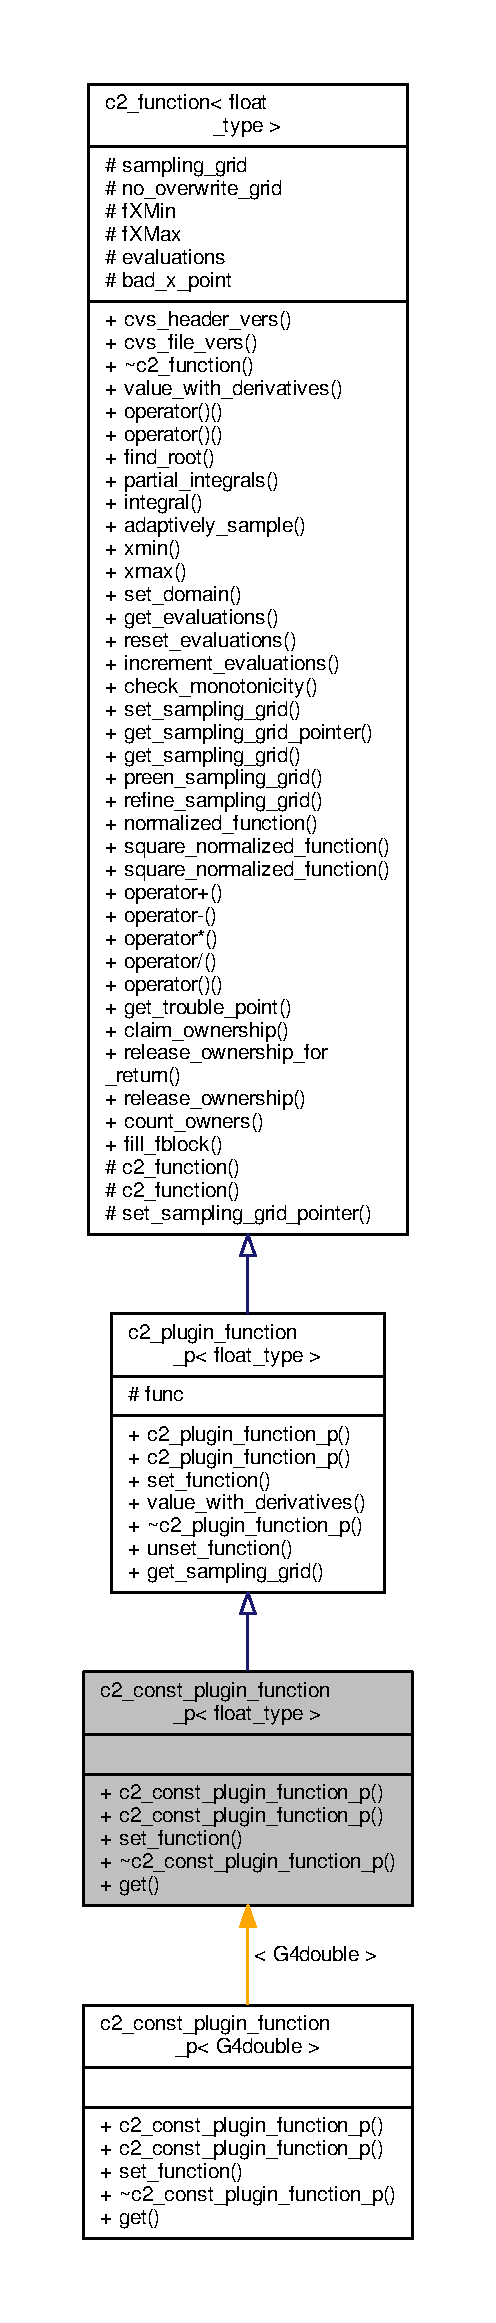
\includegraphics[height=550pt]{classc2__const__plugin__function__p__inherit__graph}
\end{center}
\end{figure}


Collaboration diagram for c2\+\_\+const\+\_\+plugin\+\_\+function\+\_\+p$<$ float\+\_\+type $>$\+:
\nopagebreak
\begin{figure}[H]
\begin{center}
\leavevmode
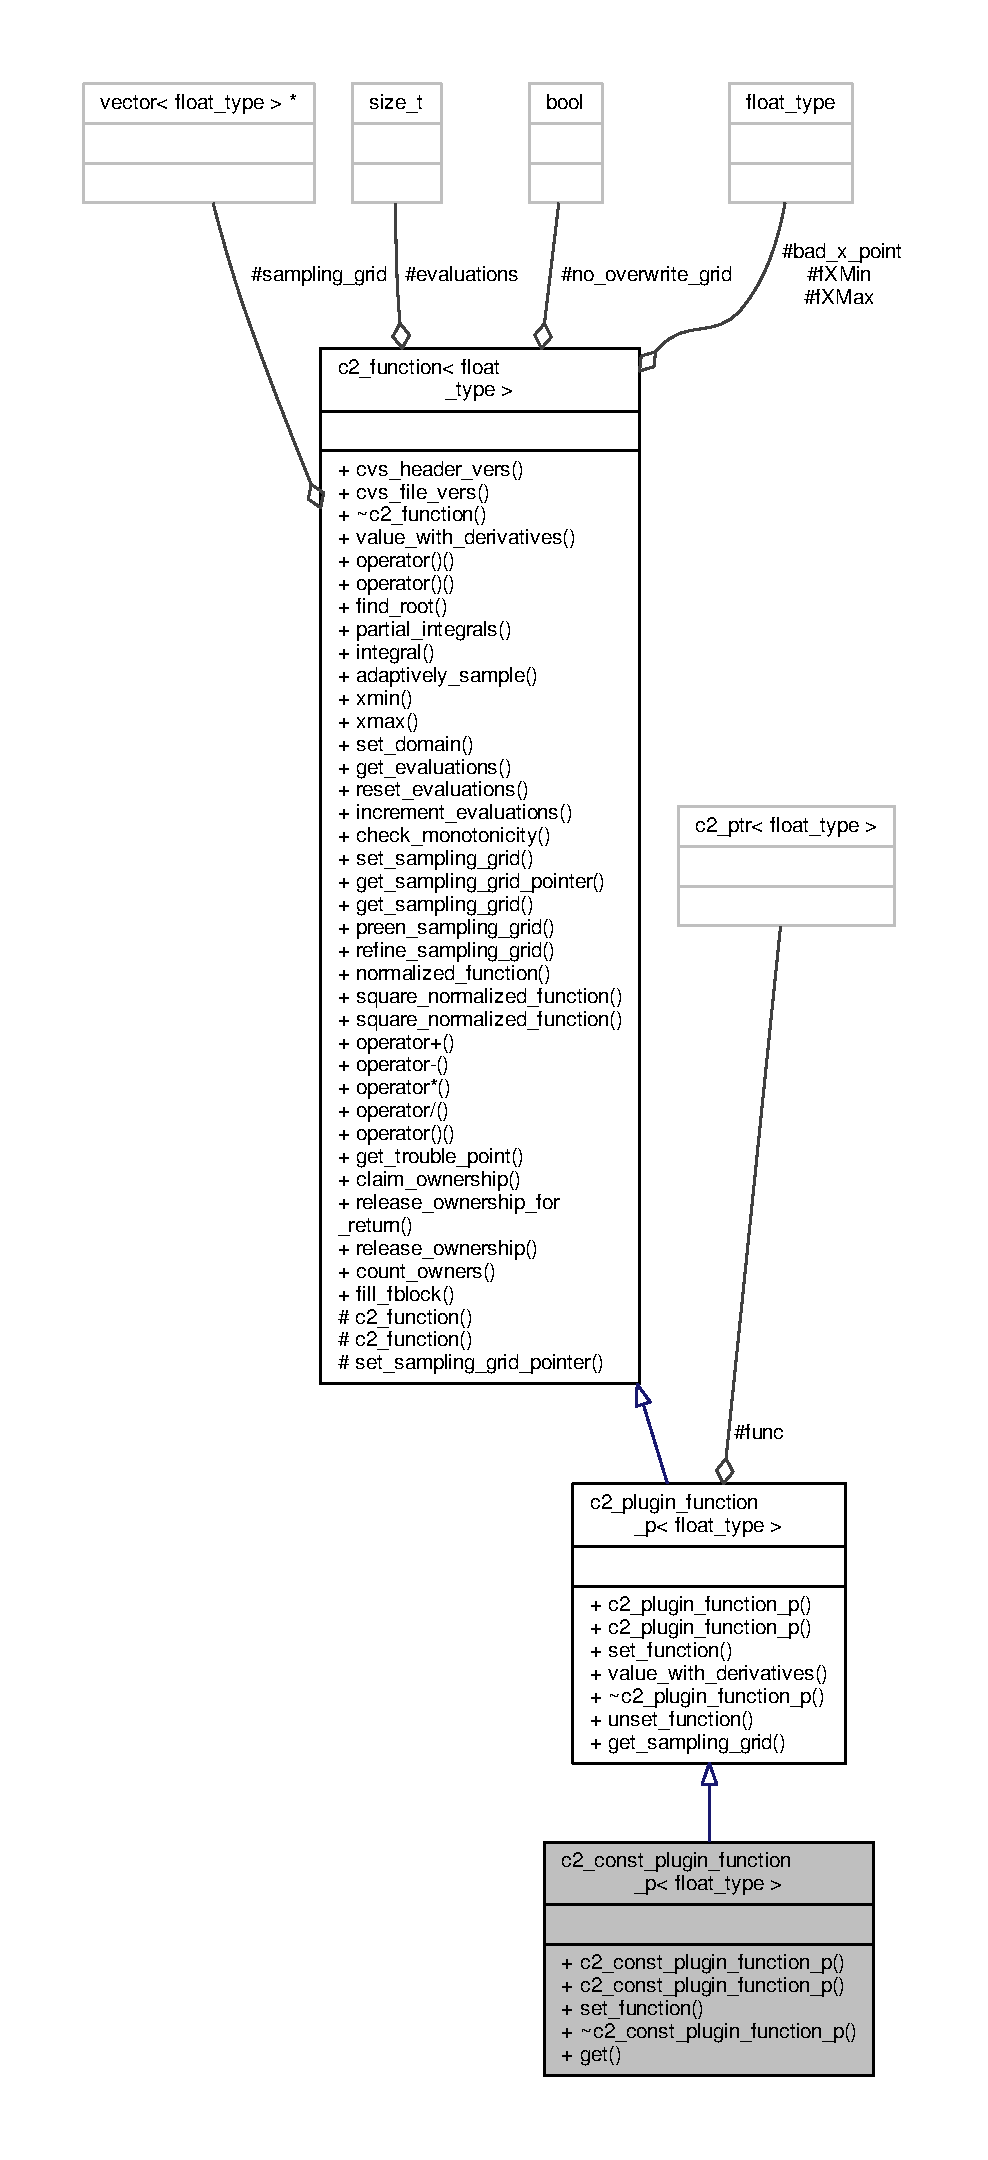
\includegraphics[height=550pt]{classc2__const__plugin__function__p__coll__graph}
\end{center}
\end{figure}
\subsection*{Public Member Functions}
\begin{DoxyCompactItemize}
\item 
\hyperlink{classc2__const__plugin__function__p_a443dc7bcbdc6e458673b98aedf53ad56}{c2\+\_\+const\+\_\+plugin\+\_\+function\+\_\+p} ()
\begin{DoxyCompactList}\small\item\em construct the container with no function \end{DoxyCompactList}\item 
\hyperlink{classc2__const__plugin__function__p_a61e0b34f7740fc05a9290f25c0615214}{c2\+\_\+const\+\_\+plugin\+\_\+function\+\_\+p} (const \hyperlink{classc2__function}{c2\+\_\+function}$<$ float\+\_\+type $>$ \&f)
\begin{DoxyCompactList}\small\item\em construct the container with a pre-\/defined function \end{DoxyCompactList}\item 
void \hyperlink{classc2__const__plugin__function__p_ab77027bb14278d0f9e49f661f784fdb5}{set\+\_\+function} (const \hyperlink{classc2__function}{c2\+\_\+function}$<$ float\+\_\+type $>$ $\ast$f)
\begin{DoxyCompactList}\small\item\em fill the container with a new function, or clear it with a null pointer \end{DoxyCompactList}\item 
virtual \hyperlink{classc2__const__plugin__function__p_a9b26b8f7469d38ff816b9a3d9b137745}{$\sim$c2\+\_\+const\+\_\+plugin\+\_\+function\+\_\+p} ()
\begin{DoxyCompactList}\small\item\em destructor \end{DoxyCompactList}\item 
const \hyperlink{classc2__function}{c2\+\_\+function}$<$ float\+\_\+type $>$ \& \hyperlink{classc2__const__plugin__function__p_ad754d7ac308b8ae26a83c61ba2c26df2}{get} () const   throw (c2\+\_\+exception)
\begin{DoxyCompactList}\small\item\em get a const reference to our owned function, for direct access \end{DoxyCompactList}\end{DoxyCompactItemize}
\subsection*{Additional Inherited Members}


\subsection{Detailed Description}
\subsubsection*{template$<$typename float\+\_\+type = double$>$\\*
class c2\+\_\+const\+\_\+plugin\+\_\+function\+\_\+p$<$ float\+\_\+type $>$}

a \hyperlink{classc2__plugin__function__p}{c2\+\_\+plugin\+\_\+function\+\_\+p} which promises not to fiddle with the plugged function.

The factory function \hyperlink{classc2__factory_aebeb20651a347e1fa8f14118faf2588e}{c2\+\_\+factory\+::const\+\_\+plugin\+\_\+function()} creates $\ast$new \hyperlink{classc2__const__plugin__function__p_a443dc7bcbdc6e458673b98aedf53ad56}{c2\+\_\+const\+\_\+plugin\+\_\+function\+\_\+p()} 

\subsection{Constructor \& Destructor Documentation}
\index{c2\+\_\+const\+\_\+plugin\+\_\+function\+\_\+p@{c2\+\_\+const\+\_\+plugin\+\_\+function\+\_\+p}!c2\+\_\+const\+\_\+plugin\+\_\+function\+\_\+p@{c2\+\_\+const\+\_\+plugin\+\_\+function\+\_\+p}}
\index{c2\+\_\+const\+\_\+plugin\+\_\+function\+\_\+p@{c2\+\_\+const\+\_\+plugin\+\_\+function\+\_\+p}!c2\+\_\+const\+\_\+plugin\+\_\+function\+\_\+p@{c2\+\_\+const\+\_\+plugin\+\_\+function\+\_\+p}}
\subsubsection[{\texorpdfstring{c2\+\_\+const\+\_\+plugin\+\_\+function\+\_\+p()}{c2_const_plugin_function_p()}}]{\setlength{\rightskip}{0pt plus 5cm}template$<$typename float\+\_\+type = double$>$ {\bf c2\+\_\+const\+\_\+plugin\+\_\+function\+\_\+p}$<$ float\+\_\+type $>$\+::{\bf c2\+\_\+const\+\_\+plugin\+\_\+function\+\_\+p} (
\begin{DoxyParamCaption}
{}
\end{DoxyParamCaption}
)\hspace{0.3cm}{\ttfamily [inline]}}\hypertarget{classc2__const__plugin__function__p_a443dc7bcbdc6e458673b98aedf53ad56}{}\label{classc2__const__plugin__function__p_a443dc7bcbdc6e458673b98aedf53ad56}


construct the container with no function 

\index{c2\+\_\+const\+\_\+plugin\+\_\+function\+\_\+p@{c2\+\_\+const\+\_\+plugin\+\_\+function\+\_\+p}!c2\+\_\+const\+\_\+plugin\+\_\+function\+\_\+p@{c2\+\_\+const\+\_\+plugin\+\_\+function\+\_\+p}}
\index{c2\+\_\+const\+\_\+plugin\+\_\+function\+\_\+p@{c2\+\_\+const\+\_\+plugin\+\_\+function\+\_\+p}!c2\+\_\+const\+\_\+plugin\+\_\+function\+\_\+p@{c2\+\_\+const\+\_\+plugin\+\_\+function\+\_\+p}}
\subsubsection[{\texorpdfstring{c2\+\_\+const\+\_\+plugin\+\_\+function\+\_\+p(const c2\+\_\+function$<$ float\+\_\+type $>$ \&f)}{c2_const_plugin_function_p(const c2_function< float_type > &f)}}]{\setlength{\rightskip}{0pt plus 5cm}template$<$typename float\+\_\+type = double$>$ {\bf c2\+\_\+const\+\_\+plugin\+\_\+function\+\_\+p}$<$ float\+\_\+type $>$\+::{\bf c2\+\_\+const\+\_\+plugin\+\_\+function\+\_\+p} (
\begin{DoxyParamCaption}
\item[{const {\bf c2\+\_\+function}$<$ float\+\_\+type $>$ \&}]{f}
\end{DoxyParamCaption}
)\hspace{0.3cm}{\ttfamily [inline]}}\hypertarget{classc2__const__plugin__function__p_a61e0b34f7740fc05a9290f25c0615214}{}\label{classc2__const__plugin__function__p_a61e0b34f7740fc05a9290f25c0615214}


construct the container with a pre-\/defined function 

\index{c2\+\_\+const\+\_\+plugin\+\_\+function\+\_\+p@{c2\+\_\+const\+\_\+plugin\+\_\+function\+\_\+p}!````~c2\+\_\+const\+\_\+plugin\+\_\+function\+\_\+p@{$\sim$c2\+\_\+const\+\_\+plugin\+\_\+function\+\_\+p}}
\index{````~c2\+\_\+const\+\_\+plugin\+\_\+function\+\_\+p@{$\sim$c2\+\_\+const\+\_\+plugin\+\_\+function\+\_\+p}!c2\+\_\+const\+\_\+plugin\+\_\+function\+\_\+p@{c2\+\_\+const\+\_\+plugin\+\_\+function\+\_\+p}}
\subsubsection[{\texorpdfstring{$\sim$c2\+\_\+const\+\_\+plugin\+\_\+function\+\_\+p()}{~c2_const_plugin_function_p()}}]{\setlength{\rightskip}{0pt plus 5cm}template$<$typename float\+\_\+type = double$>$ virtual {\bf c2\+\_\+const\+\_\+plugin\+\_\+function\+\_\+p}$<$ float\+\_\+type $>$\+::$\sim${\bf c2\+\_\+const\+\_\+plugin\+\_\+function\+\_\+p} (
\begin{DoxyParamCaption}
{}
\end{DoxyParamCaption}
)\hspace{0.3cm}{\ttfamily [inline]}, {\ttfamily [virtual]}}\hypertarget{classc2__const__plugin__function__p_a9b26b8f7469d38ff816b9a3d9b137745}{}\label{classc2__const__plugin__function__p_a9b26b8f7469d38ff816b9a3d9b137745}


destructor 



\subsection{Member Function Documentation}
\index{c2\+\_\+const\+\_\+plugin\+\_\+function\+\_\+p@{c2\+\_\+const\+\_\+plugin\+\_\+function\+\_\+p}!get@{get}}
\index{get@{get}!c2\+\_\+const\+\_\+plugin\+\_\+function\+\_\+p@{c2\+\_\+const\+\_\+plugin\+\_\+function\+\_\+p}}
\subsubsection[{\texorpdfstring{get() const }{get() const }}]{\setlength{\rightskip}{0pt plus 5cm}template$<$typename float\+\_\+type = double$>$ const {\bf c2\+\_\+function}$<$float\+\_\+type$>$\& {\bf c2\+\_\+const\+\_\+plugin\+\_\+function\+\_\+p}$<$ float\+\_\+type $>$\+::get (
\begin{DoxyParamCaption}
{}
\end{DoxyParamCaption}
) const throw  {\bf c2\+\_\+exception}) \hspace{0.3cm}{\ttfamily [inline]}}\hypertarget{classc2__const__plugin__function__p_ad754d7ac308b8ae26a83c61ba2c26df2}{}\label{classc2__const__plugin__function__p_ad754d7ac308b8ae26a83c61ba2c26df2}


get a const reference to our owned function, for direct access 

\index{c2\+\_\+const\+\_\+plugin\+\_\+function\+\_\+p@{c2\+\_\+const\+\_\+plugin\+\_\+function\+\_\+p}!set\+\_\+function@{set\+\_\+function}}
\index{set\+\_\+function@{set\+\_\+function}!c2\+\_\+const\+\_\+plugin\+\_\+function\+\_\+p@{c2\+\_\+const\+\_\+plugin\+\_\+function\+\_\+p}}
\subsubsection[{\texorpdfstring{set\+\_\+function(const c2\+\_\+function$<$ float\+\_\+type $>$ $\ast$f)}{set_function(const c2_function< float_type > *f)}}]{\setlength{\rightskip}{0pt plus 5cm}template$<$typename float\+\_\+type = double$>$ void {\bf c2\+\_\+const\+\_\+plugin\+\_\+function\+\_\+p}$<$ float\+\_\+type $>$\+::set\+\_\+function (
\begin{DoxyParamCaption}
\item[{const {\bf c2\+\_\+function}$<$ float\+\_\+type $>$ $\ast$}]{f}
\end{DoxyParamCaption}
)\hspace{0.3cm}{\ttfamily [inline]}}\hypertarget{classc2__const__plugin__function__p_ab77027bb14278d0f9e49f661f784fdb5}{}\label{classc2__const__plugin__function__p_ab77027bb14278d0f9e49f661f784fdb5}


fill the container with a new function, or clear it with a null pointer 



The documentation for this class was generated from the following file\+:\begin{DoxyCompactItemize}
\item 
\hyperlink{c2__function_8hh}{c2\+\_\+function.\+hh}\end{DoxyCompactItemize}

\hypertarget{classc2__const__ptr}{\section{c2\-\_\-const\-\_\-ptr$<$ float\-\_\-type $>$ Class Template Reference}
\label{classc2__const__ptr}\index{c2\-\_\-const\-\_\-ptr$<$ float\-\_\-type $>$@{c2\-\_\-const\-\_\-ptr$<$ float\-\_\-type $>$}}
}


create a container for a \hyperlink{classc2__function}{c2\-\_\-function} which handles the reference counting.

It is useful as a smart container to hold a \hyperlink{classc2__function}{c2\-\_\-function} and keep the reference count correct. The recommended way for a class to store a \hyperlink{classc2__function}{c2\-\_\-function} which is handed in from the outside is for it to have a \hyperlink{classc2__ptr}{c2\-\_\-ptr} member into which the passed-\/in function is stored. This way, when the class instance is deleted, it will automatically dereference any function which it was handed.  




{\ttfamily \#include $<$c2\-\_\-function.\-hh$>$}

Inheritance diagram for c2\-\_\-const\-\_\-ptr$<$ float\-\_\-type $>$\-:\begin{figure}[H]
\begin{center}
\leavevmode
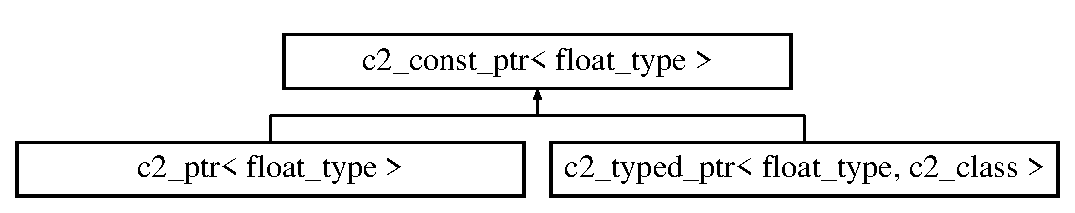
\includegraphics[height=2.000000cm]{classc2__const__ptr}
\end{center}
\end{figure}
\subsection*{Public Member Functions}
\begin{DoxyCompactItemize}
\item 
\hypertarget{classc2__const__ptr_a1f5f7e263b82efb9aa96e476c6ec21b1}{\hyperlink{classc2__const__ptr_a1f5f7e263b82efb9aa96e476c6ec21b1}{c2\-\_\-const\-\_\-ptr} ()}\label{classc2__const__ptr_a1f5f7e263b82efb9aa96e476c6ec21b1}

\begin{DoxyCompactList}\small\item\em construct the container with no function \end{DoxyCompactList}\item 
\hyperlink{classc2__const__ptr_a06e14fd555170fcd7c86ab7677961238}{c2\-\_\-const\-\_\-ptr} (const \hyperlink{classc2__function}{c2\-\_\-function}$<$ float\-\_\-type $>$ \&f)
\begin{DoxyCompactList}\small\item\em construct the container with a pre-\/defined function \end{DoxyCompactList}\item 
\hyperlink{classc2__const__ptr_abb60c8d3e444068e5ab618389dc0b82a}{c2\-\_\-const\-\_\-ptr} (const \hyperlink{classc2__const__ptr}{c2\-\_\-const\-\_\-ptr}$<$ float\-\_\-type $>$ \&src)
\begin{DoxyCompactList}\small\item\em copy constructor \end{DoxyCompactList}\item 
void \hyperlink{classc2__const__ptr_a2c7da9e9a936d57b2fb1a3cc7c636523}{set\-\_\-function} (const \hyperlink{classc2__function}{c2\-\_\-function}$<$ float\-\_\-type $>$ $\ast$f)
\begin{DoxyCompactList}\small\item\em fill the container with a new function, or clear it with a null pointer \end{DoxyCompactList}\item 
const \hyperlink{classc2__const__ptr}{c2\-\_\-const\-\_\-ptr}$<$ float\-\_\-type $>$ \& \hyperlink{classc2__const__ptr_a85155ba3652c0a1cba0a6d67d7b386dc}{operator=} (const \hyperlink{classc2__const__ptr}{c2\-\_\-const\-\_\-ptr}$<$ float\-\_\-type $>$ \&f)
\begin{DoxyCompactList}\small\item\em fill the container from another container \end{DoxyCompactList}\item 
const \hyperlink{classc2__function}{c2\-\_\-function}$<$ float\-\_\-type $>$ \& \hyperlink{classc2__const__ptr_a583d8d415ddcad806bbeb09f62ec6df6}{operator=} (const \hyperlink{classc2__function}{c2\-\_\-function}$<$ float\-\_\-type $>$ \&f)
\begin{DoxyCompactList}\small\item\em fill the container with a function \end{DoxyCompactList}\item 
void \hyperlink{classc2__const__ptr_a278e797ec2e770eaa80e84eb615819ac}{release\-\_\-for\-\_\-return} ()  throw (c2\-\_\-exception)
\begin{DoxyCompactList}\small\item\em release the function without destroying it, so it can be returned from a function \end{DoxyCompactList}\item 
void \hyperlink{classc2__const__ptr_aee1890c1f880174b9859d627d2c79425}{unset\-\_\-function} (void)
\begin{DoxyCompactList}\small\item\em clear the function \end{DoxyCompactList}\item 
\hypertarget{classc2__const__ptr_a13ec57f307039d21c12b20ab4aafda2f}{\hyperlink{classc2__const__ptr_a13ec57f307039d21c12b20ab4aafda2f}{$\sim$c2\-\_\-const\-\_\-ptr} ()}\label{classc2__const__ptr_a13ec57f307039d21c12b20ab4aafda2f}

\begin{DoxyCompactList}\small\item\em destructor \end{DoxyCompactList}\item 
\hypertarget{classc2__const__ptr_a6d9dd4874c62d571d4d016f2de4a8aeb}{const \hyperlink{classc2__function}{c2\-\_\-function}$<$ float\-\_\-type $>$ \& \hyperlink{classc2__const__ptr_a6d9dd4874c62d571d4d016f2de4a8aeb}{get} () const   throw (c2\-\_\-exception)}\label{classc2__const__ptr_a6d9dd4874c62d571d4d016f2de4a8aeb}

\begin{DoxyCompactList}\small\item\em get a reference to our owned function \end{DoxyCompactList}\item 
\hypertarget{classc2__const__ptr_a63812c6959fbef01ade67dfeff760341}{const \hyperlink{classc2__function}{c2\-\_\-function}$<$ float\-\_\-type $>$ $\ast$ \hyperlink{classc2__const__ptr_a63812c6959fbef01ade67dfeff760341}{get\-\_\-ptr} () const }\label{classc2__const__ptr_a63812c6959fbef01ade67dfeff760341}

\begin{DoxyCompactList}\small\item\em get an unchecked pointer to our owned function \end{DoxyCompactList}\item 
\hypertarget{classc2__const__ptr_a1a15e6786744bcebbe3bc8f0d53ad79d}{const \hyperlink{classc2__function}{c2\-\_\-function}$<$ float\-\_\-type $>$ $\ast$ \hyperlink{classc2__const__ptr_a1a15e6786744bcebbe3bc8f0d53ad79d}{operator-\/$>$} () const }\label{classc2__const__ptr_a1a15e6786744bcebbe3bc8f0d53ad79d}

\begin{DoxyCompactList}\small\item\em get a checked pointer to our owned function \end{DoxyCompactList}\item 
\hypertarget{classc2__const__ptr_a658dc06f2a368d0fb0514b460d222863}{bool \hyperlink{classc2__const__ptr_a658dc06f2a368d0fb0514b460d222863}{valid} () const }\label{classc2__const__ptr_a658dc06f2a368d0fb0514b460d222863}

\begin{DoxyCompactList}\small\item\em check if we have a valid function \end{DoxyCompactList}\item 
\hypertarget{classc2__const__ptr_a504b8baffa3de2180d200aa7bfcaaa3e}{\hyperlink{classc2__const__ptr_a504b8baffa3de2180d200aa7bfcaaa3e}{operator const c2\-\_\-function$<$ float\-\_\-type $>$ \&} () const }\label{classc2__const__ptr_a504b8baffa3de2180d200aa7bfcaaa3e}

\begin{DoxyCompactList}\small\item\em type coercion operator which lets us use a pointer as if it were a const \hyperlink{classc2__function}{c2\-\_\-function} \end{DoxyCompactList}\item 
float\-\_\-type \hyperlink{classc2__const__ptr_a7c9a4582f4ddb5eee68a8ebbd14b4280}{operator()} (float\-\_\-type x) const   throw (c2\-\_\-exception)
\begin{DoxyCompactList}\small\item\em convenience operator to make us look like a function \end{DoxyCompactList}\item 
float\-\_\-type \hyperlink{classc2__const__ptr_accdc2e24cc09242d3ded1b7a22ae803e}{operator()} (float\-\_\-type x, float\-\_\-type $\ast$yprime, float\-\_\-type $\ast$yprime2) const   throw (c2\-\_\-exception)
\begin{DoxyCompactList}\small\item\em convenience operator to make us look like a function \end{DoxyCompactList}\item 
\hyperlink{classc2__sum__p}{c2\-\_\-sum\-\_\-p}$<$ float\-\_\-type $>$ \& \hyperlink{classc2__const__ptr_ad93bdeb0b0e78f31ce4fa4b83b38cf27}{operator+} (const \hyperlink{classc2__function}{c2\-\_\-function}$<$ float\-\_\-type $>$ \&rhs) const   throw (c2\-\_\-exception)
\begin{DoxyCompactList}\small\item\em factory function to create a \hyperlink{classc2__sum__p}{c2\-\_\-sum\-\_\-p} from a regular algebraic expression. \end{DoxyCompactList}\item 
\hyperlink{classc2__diff__p}{c2\-\_\-diff\-\_\-p}$<$ float\-\_\-type $>$ \& \hyperlink{classc2__const__ptr_ac2bc3992872343e2160040631ab43ffe}{operator-\/} (const \hyperlink{classc2__function}{c2\-\_\-function}$<$ float\-\_\-type $>$ \&rhs) const   throw (c2\-\_\-exception)
\begin{DoxyCompactList}\small\item\em factory function to create a \hyperlink{classc2__diff__p}{c2\-\_\-diff\-\_\-p} from a regular algebraic expression. \end{DoxyCompactList}\item 
\hyperlink{classc2__product__p}{c2\-\_\-product\-\_\-p}$<$ float\-\_\-type $>$ \& \hyperlink{classc2__const__ptr_a7be0220692df9d2118a14ee855d617be}{operator$\ast$} (const \hyperlink{classc2__function}{c2\-\_\-function}$<$ float\-\_\-type $>$ \&rhs) const   throw (c2\-\_\-exception)
\begin{DoxyCompactList}\small\item\em factory function to create a \hyperlink{classc2__product__p}{c2\-\_\-product\-\_\-p} from a regular algebraic expression. \end{DoxyCompactList}\item 
\hyperlink{classc2__ratio__p}{c2\-\_\-ratio\-\_\-p}$<$ float\-\_\-type $>$ \& \hyperlink{classc2__const__ptr_ae3487ff977e84cd98e0ae1c495903766}{operator/} (const \hyperlink{classc2__function}{c2\-\_\-function}$<$ float\-\_\-type $>$ \&rhs) const   throw (c2\-\_\-exception)
\begin{DoxyCompactList}\small\item\em factory function to create a \hyperlink{classc2__ratio__p}{c2\-\_\-ratio\-\_\-p} from a regular algebraic expression. \end{DoxyCompactList}\item 
\hyperlink{classc2__composed__function__p}{c2\-\_\-composed\-\_\-function\-\_\-p}\\*
$<$ float\-\_\-type $>$ \& \hyperlink{classc2__const__ptr_a0fc370d82f1077fa7054e1a10a93ed6c}{operator()} (const \hyperlink{classc2__function}{c2\-\_\-function}$<$ float\-\_\-type $>$ \&inner) const   throw (c2\-\_\-exception)
\begin{DoxyCompactList}\small\item\em compose this function outside another. \end{DoxyCompactList}\end{DoxyCompactItemize}
\subsection*{Protected Attributes}
\begin{DoxyCompactItemize}
\item 
\hypertarget{classc2__const__ptr_a6de6b341a9e28137557dbe496813e415}{const \hyperlink{classc2__function}{c2\-\_\-function}$<$ float\-\_\-type $>$ $\ast$ {\bfseries func}}\label{classc2__const__ptr_a6de6b341a9e28137557dbe496813e415}

\end{DoxyCompactItemize}


\subsection{Detailed Description}
\subsubsection*{template$<$typename float\-\_\-type$>$class c2\-\_\-const\-\_\-ptr$<$ float\-\_\-type $>$}

create a container for a \hyperlink{classc2__function}{c2\-\_\-function} which handles the reference counting.

It is useful as a smart container to hold a \hyperlink{classc2__function}{c2\-\_\-function} and keep the reference count correct. The recommended way for a class to store a \hyperlink{classc2__function}{c2\-\_\-function} which is handed in from the outside is for it to have a \hyperlink{classc2__ptr}{c2\-\_\-ptr} member into which the passed-\/in function is stored. This way, when the class instance is deleted, it will automatically dereference any function which it was handed. 

This class contains a copy constructor and operator=, to make it fairly easy to make a std\-::vector of these objects, and have it work as expected. 

\subsection{Constructor \& Destructor Documentation}
\hypertarget{classc2__const__ptr_a06e14fd555170fcd7c86ab7677961238}{\index{c2\-\_\-const\-\_\-ptr@{c2\-\_\-const\-\_\-ptr}!c2\-\_\-const\-\_\-ptr@{c2\-\_\-const\-\_\-ptr}}
\index{c2\-\_\-const\-\_\-ptr@{c2\-\_\-const\-\_\-ptr}!c2_const_ptr@{c2\-\_\-const\-\_\-ptr}}
\subsubsection[{c2\-\_\-const\-\_\-ptr}]{\setlength{\rightskip}{0pt plus 5cm}template$<$typename float\-\_\-type$>$ {\bf c2\-\_\-const\-\_\-ptr}$<$ float\-\_\-type $>$\-::{\bf c2\-\_\-const\-\_\-ptr} (
\begin{DoxyParamCaption}
\item[{const {\bf c2\-\_\-function}$<$ float\-\_\-type $>$ \&}]{f}
\end{DoxyParamCaption}
)\hspace{0.3cm}{\ttfamily [inline]}}}\label{classc2__const__ptr_a06e14fd555170fcd7c86ab7677961238}


construct the container with a pre-\/defined function 


\begin{DoxyParams}{Parameters}
{\em f} & the function to store \\
\hline
\end{DoxyParams}
\hypertarget{classc2__const__ptr_abb60c8d3e444068e5ab618389dc0b82a}{\index{c2\-\_\-const\-\_\-ptr@{c2\-\_\-const\-\_\-ptr}!c2\-\_\-const\-\_\-ptr@{c2\-\_\-const\-\_\-ptr}}
\index{c2\-\_\-const\-\_\-ptr@{c2\-\_\-const\-\_\-ptr}!c2_const_ptr@{c2\-\_\-const\-\_\-ptr}}
\subsubsection[{c2\-\_\-const\-\_\-ptr}]{\setlength{\rightskip}{0pt plus 5cm}template$<$typename float\-\_\-type$>$ {\bf c2\-\_\-const\-\_\-ptr}$<$ float\-\_\-type $>$\-::{\bf c2\-\_\-const\-\_\-ptr} (
\begin{DoxyParamCaption}
\item[{const {\bf c2\-\_\-const\-\_\-ptr}$<$ float\-\_\-type $>$ \&}]{src}
\end{DoxyParamCaption}
)\hspace{0.3cm}{\ttfamily [inline]}}}\label{classc2__const__ptr_abb60c8d3e444068e5ab618389dc0b82a}


copy constructor 


\begin{DoxyParams}{Parameters}
{\em src} & the container to copy \\
\hline
\end{DoxyParams}


\subsection{Member Function Documentation}
\hypertarget{classc2__const__ptr_a7c9a4582f4ddb5eee68a8ebbd14b4280}{\index{c2\-\_\-const\-\_\-ptr@{c2\-\_\-const\-\_\-ptr}!operator()@{operator()}}
\index{operator()@{operator()}!c2_const_ptr@{c2\-\_\-const\-\_\-ptr}}
\subsubsection[{operator()}]{\setlength{\rightskip}{0pt plus 5cm}template$<$typename float\-\_\-type$>$ float\-\_\-type {\bf c2\-\_\-const\-\_\-ptr}$<$ float\-\_\-type $>$\-::operator() (
\begin{DoxyParamCaption}
\item[{float\-\_\-type}]{x}
\end{DoxyParamCaption}
) const throw  {\bf c2\-\_\-exception}) \hspace{0.3cm}{\ttfamily [inline]}}}\label{classc2__const__ptr_a7c9a4582f4ddb5eee68a8ebbd14b4280}


convenience operator to make us look like a function 


\begin{DoxyParams}{Parameters}
{\em x} & the value at which to evaluate the contained function \\
\hline
\end{DoxyParams}
\begin{DoxyReturn}{Returns}
the evaluated function 
\end{DoxyReturn}
\begin{DoxyNote}{Note}
If you using this repeatedly, do const c2\-\_\-function$<$float\-\_\-type$>$ \&func=ptr; and use func(x). Calling this operator wastes some time, since it checks the validity of the pointer every time. 
\end{DoxyNote}
\hypertarget{classc2__const__ptr_accdc2e24cc09242d3ded1b7a22ae803e}{\index{c2\-\_\-const\-\_\-ptr@{c2\-\_\-const\-\_\-ptr}!operator()@{operator()}}
\index{operator()@{operator()}!c2_const_ptr@{c2\-\_\-const\-\_\-ptr}}
\subsubsection[{operator()}]{\setlength{\rightskip}{0pt plus 5cm}template$<$typename float\-\_\-type$>$ float\-\_\-type {\bf c2\-\_\-const\-\_\-ptr}$<$ float\-\_\-type $>$\-::operator() (
\begin{DoxyParamCaption}
\item[{float\-\_\-type}]{x, }
\item[{float\-\_\-type $\ast$}]{yprime, }
\item[{float\-\_\-type $\ast$}]{yprime2}
\end{DoxyParamCaption}
) const throw  {\bf c2\-\_\-exception}) \hspace{0.3cm}{\ttfamily [inline]}}}\label{classc2__const__ptr_accdc2e24cc09242d3ded1b7a22ae803e}


convenience operator to make us look like a function 


\begin{DoxyParams}{Parameters}
{\em x} & the value at which to evaluate the contained function \\
\hline
{\em yprime} & the derivative \\
\hline
{\em yprime2} & the second derivative \\
\hline
\end{DoxyParams}
\begin{DoxyReturn}{Returns}
the evaluated function 
\end{DoxyReturn}
\begin{DoxyNote}{Note}
If you using this repeatedly, do const c2\-\_\-function$<$float\-\_\-type$>$ \&func=ptr; and use func(x). Calling this operator wastes some time, since it checks the validity of the pointer every time. 
\end{DoxyNote}
\hypertarget{classc2__const__ptr_a0fc370d82f1077fa7054e1a10a93ed6c}{\index{c2\-\_\-const\-\_\-ptr@{c2\-\_\-const\-\_\-ptr}!operator()@{operator()}}
\index{operator()@{operator()}!c2_const_ptr@{c2\-\_\-const\-\_\-ptr}}
\subsubsection[{operator()}]{\setlength{\rightskip}{0pt plus 5cm}template$<$typename float\-\_\-type$>$ {\bf c2\-\_\-composed\-\_\-function\-\_\-p}$<$float\-\_\-type$>$\& {\bf c2\-\_\-const\-\_\-ptr}$<$ float\-\_\-type $>$\-::operator() (
\begin{DoxyParamCaption}
\item[{const {\bf c2\-\_\-function}$<$ float\-\_\-type $>$ \&}]{inner}
\end{DoxyParamCaption}
) const throw  {\bf c2\-\_\-exception}) \hspace{0.3cm}{\ttfamily [inline]}}}\label{classc2__const__ptr_a0fc370d82f1077fa7054e1a10a93ed6c}


compose this function outside another. 


\begin{DoxyParams}{Parameters}
{\em inner} & the inner function \\
\hline
\end{DoxyParams}
\begin{DoxyReturn}{Returns}
the composed function 
\end{DoxyReturn}
\hypertarget{classc2__const__ptr_a7be0220692df9d2118a14ee855d617be}{\index{c2\-\_\-const\-\_\-ptr@{c2\-\_\-const\-\_\-ptr}!operator$\ast$@{operator$\ast$}}
\index{operator$\ast$@{operator$\ast$}!c2_const_ptr@{c2\-\_\-const\-\_\-ptr}}
\subsubsection[{operator$\ast$}]{\setlength{\rightskip}{0pt plus 5cm}template$<$typename float\-\_\-type$>$ {\bf c2\-\_\-product\-\_\-p}$<$float\-\_\-type$>$\& {\bf c2\-\_\-const\-\_\-ptr}$<$ float\-\_\-type $>$\-::operator$\ast$ (
\begin{DoxyParamCaption}
\item[{const {\bf c2\-\_\-function}$<$ float\-\_\-type $>$ \&}]{rhs}
\end{DoxyParamCaption}
) const throw  {\bf c2\-\_\-exception}) \hspace{0.3cm}{\ttfamily [inline]}}}\label{classc2__const__ptr_a7be0220692df9d2118a14ee855d617be}


factory function to create a \hyperlink{classc2__product__p}{c2\-\_\-product\-\_\-p} from a regular algebraic expression. 


\begin{DoxyParams}{Parameters}
{\em rhs} & the right-\/hand term of the product \\
\hline
\end{DoxyParams}
\begin{DoxyReturn}{Returns}
a new \hyperlink{classc2__function}{c2\-\_\-function} 
\end{DoxyReturn}
\hypertarget{classc2__const__ptr_ad93bdeb0b0e78f31ce4fa4b83b38cf27}{\index{c2\-\_\-const\-\_\-ptr@{c2\-\_\-const\-\_\-ptr}!operator+@{operator+}}
\index{operator+@{operator+}!c2_const_ptr@{c2\-\_\-const\-\_\-ptr}}
\subsubsection[{operator+}]{\setlength{\rightskip}{0pt plus 5cm}template$<$typename float\-\_\-type$>$ {\bf c2\-\_\-sum\-\_\-p}$<$float\-\_\-type$>$\& {\bf c2\-\_\-const\-\_\-ptr}$<$ float\-\_\-type $>$\-::operator+ (
\begin{DoxyParamCaption}
\item[{const {\bf c2\-\_\-function}$<$ float\-\_\-type $>$ \&}]{rhs}
\end{DoxyParamCaption}
) const throw  {\bf c2\-\_\-exception}) \hspace{0.3cm}{\ttfamily [inline]}}}\label{classc2__const__ptr_ad93bdeb0b0e78f31ce4fa4b83b38cf27}


factory function to create a \hyperlink{classc2__sum__p}{c2\-\_\-sum\-\_\-p} from a regular algebraic expression. 


\begin{DoxyParams}{Parameters}
{\em rhs} & the right-\/hand term of the sum \\
\hline
\end{DoxyParams}
\begin{DoxyReturn}{Returns}
a new \hyperlink{classc2__function}{c2\-\_\-function} 
\end{DoxyReturn}
\hypertarget{classc2__const__ptr_ac2bc3992872343e2160040631ab43ffe}{\index{c2\-\_\-const\-\_\-ptr@{c2\-\_\-const\-\_\-ptr}!operator-\/@{operator-\/}}
\index{operator-\/@{operator-\/}!c2_const_ptr@{c2\-\_\-const\-\_\-ptr}}
\subsubsection[{operator-\/}]{\setlength{\rightskip}{0pt plus 5cm}template$<$typename float\-\_\-type$>$ {\bf c2\-\_\-diff\-\_\-p}$<$float\-\_\-type$>$\& {\bf c2\-\_\-const\-\_\-ptr}$<$ float\-\_\-type $>$\-::operator-\/ (
\begin{DoxyParamCaption}
\item[{const {\bf c2\-\_\-function}$<$ float\-\_\-type $>$ \&}]{rhs}
\end{DoxyParamCaption}
) const throw  {\bf c2\-\_\-exception}) \hspace{0.3cm}{\ttfamily [inline]}}}\label{classc2__const__ptr_ac2bc3992872343e2160040631ab43ffe}


factory function to create a \hyperlink{classc2__diff__p}{c2\-\_\-diff\-\_\-p} from a regular algebraic expression. 


\begin{DoxyParams}{Parameters}
{\em rhs} & the right-\/hand term of the difference \\
\hline
\end{DoxyParams}
\begin{DoxyReturn}{Returns}
a new \hyperlink{classc2__function}{c2\-\_\-function} 
\end{DoxyReturn}
\hypertarget{classc2__const__ptr_ae3487ff977e84cd98e0ae1c495903766}{\index{c2\-\_\-const\-\_\-ptr@{c2\-\_\-const\-\_\-ptr}!operator/@{operator/}}
\index{operator/@{operator/}!c2_const_ptr@{c2\-\_\-const\-\_\-ptr}}
\subsubsection[{operator/}]{\setlength{\rightskip}{0pt plus 5cm}template$<$typename float\-\_\-type$>$ {\bf c2\-\_\-ratio\-\_\-p}$<$float\-\_\-type$>$\& {\bf c2\-\_\-const\-\_\-ptr}$<$ float\-\_\-type $>$\-::operator/ (
\begin{DoxyParamCaption}
\item[{const {\bf c2\-\_\-function}$<$ float\-\_\-type $>$ \&}]{rhs}
\end{DoxyParamCaption}
) const throw  {\bf c2\-\_\-exception}) \hspace{0.3cm}{\ttfamily [inline]}}}\label{classc2__const__ptr_ae3487ff977e84cd98e0ae1c495903766}


factory function to create a \hyperlink{classc2__ratio__p}{c2\-\_\-ratio\-\_\-p} from a regular algebraic expression. 


\begin{DoxyParams}{Parameters}
{\em rhs} & the right-\/hand term of the ratio (the denominator) \\
\hline
\end{DoxyParams}
\begin{DoxyReturn}{Returns}
a new \hyperlink{classc2__function}{c2\-\_\-function} 
\end{DoxyReturn}
\hypertarget{classc2__const__ptr_a85155ba3652c0a1cba0a6d67d7b386dc}{\index{c2\-\_\-const\-\_\-ptr@{c2\-\_\-const\-\_\-ptr}!operator=@{operator=}}
\index{operator=@{operator=}!c2_const_ptr@{c2\-\_\-const\-\_\-ptr}}
\subsubsection[{operator=}]{\setlength{\rightskip}{0pt plus 5cm}template$<$typename float\-\_\-type$>$ const {\bf c2\-\_\-const\-\_\-ptr}$<$float\-\_\-type$>$\& {\bf c2\-\_\-const\-\_\-ptr}$<$ float\-\_\-type $>$\-::operator= (
\begin{DoxyParamCaption}
\item[{const {\bf c2\-\_\-const\-\_\-ptr}$<$ float\-\_\-type $>$ \&}]{f}
\end{DoxyParamCaption}
)\hspace{0.3cm}{\ttfamily [inline]}}}\label{classc2__const__ptr_a85155ba3652c0a1cba0a6d67d7b386dc}


fill the container from another container 


\begin{DoxyParams}{Parameters}
{\em f} & the container to copy \\
\hline
\end{DoxyParams}
\hypertarget{classc2__const__ptr_a583d8d415ddcad806bbeb09f62ec6df6}{\index{c2\-\_\-const\-\_\-ptr@{c2\-\_\-const\-\_\-ptr}!operator=@{operator=}}
\index{operator=@{operator=}!c2_const_ptr@{c2\-\_\-const\-\_\-ptr}}
\subsubsection[{operator=}]{\setlength{\rightskip}{0pt plus 5cm}template$<$typename float\-\_\-type$>$ const {\bf c2\-\_\-function}$<$float\-\_\-type$>$\& {\bf c2\-\_\-const\-\_\-ptr}$<$ float\-\_\-type $>$\-::operator= (
\begin{DoxyParamCaption}
\item[{const {\bf c2\-\_\-function}$<$ float\-\_\-type $>$ \&}]{f}
\end{DoxyParamCaption}
)\hspace{0.3cm}{\ttfamily [inline]}}}\label{classc2__const__ptr_a583d8d415ddcad806bbeb09f62ec6df6}


fill the container with a function 


\begin{DoxyParams}{Parameters}
{\em f} & the function \\
\hline
\end{DoxyParams}
\hypertarget{classc2__const__ptr_a278e797ec2e770eaa80e84eb615819ac}{\index{c2\-\_\-const\-\_\-ptr@{c2\-\_\-const\-\_\-ptr}!release\-\_\-for\-\_\-return@{release\-\_\-for\-\_\-return}}
\index{release\-\_\-for\-\_\-return@{release\-\_\-for\-\_\-return}!c2_const_ptr@{c2\-\_\-const\-\_\-ptr}}
\subsubsection[{release\-\_\-for\-\_\-return}]{\setlength{\rightskip}{0pt plus 5cm}template$<$typename float\-\_\-type$>$ void {\bf c2\-\_\-const\-\_\-ptr}$<$ float\-\_\-type $>$\-::release\-\_\-for\-\_\-return (
\begin{DoxyParamCaption}
{}
\end{DoxyParamCaption}
) throw  {\bf c2\-\_\-exception}) \hspace{0.3cm}{\ttfamily [inline]}}}\label{classc2__const__ptr_a278e797ec2e770eaa80e84eb615819ac}


release the function without destroying it, so it can be returned from a function 

This is usually the very last line of a function before the return statement, so that any exceptions that happen during execution of the function will cause proper cleanup. Once the function has been released from its container this way, it is an orhpaned object until the caller claims it, so it could get lost if an exception happens. \hypertarget{classc2__const__ptr_a2c7da9e9a936d57b2fb1a3cc7c636523}{\index{c2\-\_\-const\-\_\-ptr@{c2\-\_\-const\-\_\-ptr}!set\-\_\-function@{set\-\_\-function}}
\index{set\-\_\-function@{set\-\_\-function}!c2_const_ptr@{c2\-\_\-const\-\_\-ptr}}
\subsubsection[{set\-\_\-function}]{\setlength{\rightskip}{0pt plus 5cm}template$<$typename float\-\_\-type$>$ void {\bf c2\-\_\-const\-\_\-ptr}$<$ float\-\_\-type $>$\-::set\-\_\-function (
\begin{DoxyParamCaption}
\item[{const {\bf c2\-\_\-function}$<$ float\-\_\-type $>$ $\ast$}]{f}
\end{DoxyParamCaption}
)\hspace{0.3cm}{\ttfamily [inline]}}}\label{classc2__const__ptr_a2c7da9e9a936d57b2fb1a3cc7c636523}


fill the container with a new function, or clear it with a null pointer 


\begin{DoxyParams}{Parameters}
{\em f} & the function to store, releasing any previously held function \\
\hline
\end{DoxyParams}
\hypertarget{classc2__const__ptr_aee1890c1f880174b9859d627d2c79425}{\index{c2\-\_\-const\-\_\-ptr@{c2\-\_\-const\-\_\-ptr}!unset\-\_\-function@{unset\-\_\-function}}
\index{unset\-\_\-function@{unset\-\_\-function}!c2_const_ptr@{c2\-\_\-const\-\_\-ptr}}
\subsubsection[{unset\-\_\-function}]{\setlength{\rightskip}{0pt plus 5cm}template$<$typename float\-\_\-type$>$ void {\bf c2\-\_\-const\-\_\-ptr}$<$ float\-\_\-type $>$\-::unset\-\_\-function (
\begin{DoxyParamCaption}
\item[{void}]{}
\end{DoxyParamCaption}
)\hspace{0.3cm}{\ttfamily [inline]}}}\label{classc2__const__ptr_aee1890c1f880174b9859d627d2c79425}


clear the function 

Any attempt to use this \hyperlink{classc2__plugin__function__p}{c2\-\_\-plugin\-\_\-function\-\_\-p} throws an exception if the saved function is cleared. 

The documentation for this class was generated from the following file\-:\begin{DoxyCompactItemize}
\item 
\hyperlink{c2__function_8hh}{c2\-\_\-function.\-hh}\end{DoxyCompactItemize}

\hypertarget{classc2__constant__p}{\section{c2\-\_\-constant\-\_\-p$<$ float\-\_\-type $>$ Class Template Reference}
\label{classc2__constant__p}\index{c2\-\_\-constant\-\_\-p$<$ float\-\_\-type $>$@{c2\-\_\-constant\-\_\-p$<$ float\-\_\-type $>$}}
}


a \hyperlink{classc2__function}{c2\-\_\-function} which is constant

The factory function \hyperlink{classc2__factory_a98e385b2b927d15d4376821302061d4d}{c2\-\_\-factory\-::constant()} creates $\ast$new \hyperlink{classc2__constant__p}{c2\-\_\-constant\-\_\-p()}  




{\ttfamily \#include $<$c2\-\_\-function.\-hh$>$}

Inheritance diagram for c2\-\_\-constant\-\_\-p$<$ float\-\_\-type $>$\-:\begin{figure}[H]
\begin{center}
\leavevmode
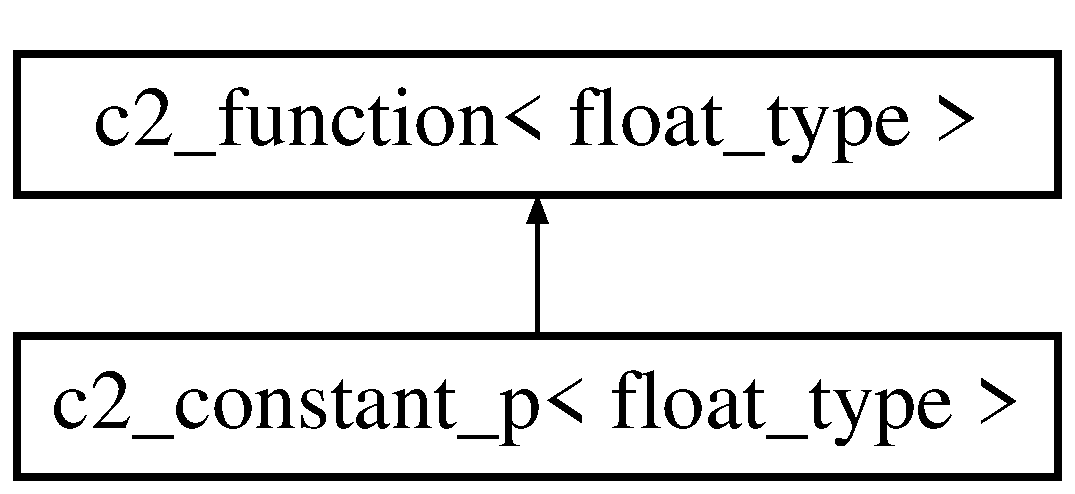
\includegraphics[height=2.000000cm]{classc2__constant__p}
\end{center}
\end{figure}
\subsection*{Public Member Functions}
\begin{DoxyCompactItemize}
\item 
\hypertarget{classc2__constant__p_ae62311ccce870ca4fb79b7c9d525a3d2}{{\bfseries c2\-\_\-constant\-\_\-p} (float\-\_\-type x)}\label{classc2__constant__p_ae62311ccce870ca4fb79b7c9d525a3d2}

\item 
\hypertarget{classc2__constant__p_a5dd45be662a8358a43e25bab057e3aa9}{void {\bfseries reset} (float\-\_\-type val)}\label{classc2__constant__p_a5dd45be662a8358a43e25bab057e3aa9}

\item 
virtual float\-\_\-type \hyperlink{classc2__constant__p_a75ec878f6eb48c5ea0187197c645dd66}{value\-\_\-with\-\_\-derivatives} (float\-\_\-type, float\-\_\-type $\ast$yprime, float\-\_\-type $\ast$yprime2) const   throw (c2\-\_\-exception)
\begin{DoxyCompactList}\small\item\em get the value and derivatives. \end{DoxyCompactList}\end{DoxyCompactItemize}
\subsection*{Additional Inherited Members}


\subsection{Detailed Description}
\subsubsection*{template$<$typename float\-\_\-type$>$class c2\-\_\-constant\-\_\-p$<$ float\-\_\-type $>$}

a \hyperlink{classc2__function}{c2\-\_\-function} which is constant

The factory function \hyperlink{classc2__factory_a98e385b2b927d15d4376821302061d4d}{c2\-\_\-factory\-::constant()} creates $\ast$new \hyperlink{classc2__constant__p}{c2\-\_\-constant\-\_\-p()} 

\subsection{Member Function Documentation}
\hypertarget{classc2__constant__p_a75ec878f6eb48c5ea0187197c645dd66}{\index{c2\-\_\-constant\-\_\-p@{c2\-\_\-constant\-\_\-p}!value\-\_\-with\-\_\-derivatives@{value\-\_\-with\-\_\-derivatives}}
\index{value\-\_\-with\-\_\-derivatives@{value\-\_\-with\-\_\-derivatives}!c2_constant_p@{c2\-\_\-constant\-\_\-p}}
\subsubsection[{value\-\_\-with\-\_\-derivatives}]{\setlength{\rightskip}{0pt plus 5cm}template$<$typename float\-\_\-type $>$ virtual float\-\_\-type {\bf c2\-\_\-constant\-\_\-p}$<$ float\-\_\-type $>$\-::value\-\_\-with\-\_\-derivatives (
\begin{DoxyParamCaption}
\item[{float\-\_\-type}]{x, }
\item[{float\-\_\-type $\ast$}]{yprime, }
\item[{float\-\_\-type $\ast$}]{yprime2}
\end{DoxyParamCaption}
) const throw  {\bf c2\-\_\-exception}) \hspace{0.3cm}{\ttfamily [inline]}, {\ttfamily [virtual]}}}\label{classc2__constant__p_a75ec878f6eb48c5ea0187197c645dd66}


get the value and derivatives. 

There is required checking for null pointers on the derivatives, and most implementations should operate faster if derivatives are not needed. 
\begin{DoxyParams}[1]{Parameters}
\mbox{\tt in}  & {\em x} & the point at which to evaluate the function \\
\hline
\mbox{\tt out}  & {\em yprime} & the first derivative (if pointer is non-\/null) \\
\hline
\mbox{\tt out}  & {\em yprime2} & the second derivative (if pointer is non-\/null) \\
\hline
\end{DoxyParams}
\begin{DoxyReturn}{Returns}
the value of the function 
\end{DoxyReturn}


Implements \hyperlink{classc2__function_a44e0201159111350be7f746fc9026f67}{c2\-\_\-function$<$ float\-\_\-type $>$}.



The documentation for this class was generated from the following file\-:\begin{DoxyCompactItemize}
\item 
\hyperlink{c2__function_8hh}{c2\-\_\-function.\-hh}\end{DoxyCompactItemize}

\hypertarget{classc2__cos__p}{\section{c2\-\_\-cos\-\_\-p$<$ float\-\_\-type $>$ Class Template Reference}
\label{classc2__cos__p}\index{c2\-\_\-cos\-\_\-p$<$ float\-\_\-type $>$@{c2\-\_\-cos\-\_\-p$<$ float\-\_\-type $>$}}
}


compute cos(x) with its derivatives.

The factory function \hyperlink{classc2__factory_abc5ea51417ecef590629a39f7a2227e4}{c2\-\_\-factory\-::cos()} creates $\ast$new \hyperlink{classc2__cos__p}{c2\-\_\-cos\-\_\-p}  




{\ttfamily \#include $<$c2\-\_\-function.\-hh$>$}

Inheritance diagram for c2\-\_\-cos\-\_\-p$<$ float\-\_\-type $>$\-:\begin{figure}[H]
\begin{center}
\leavevmode
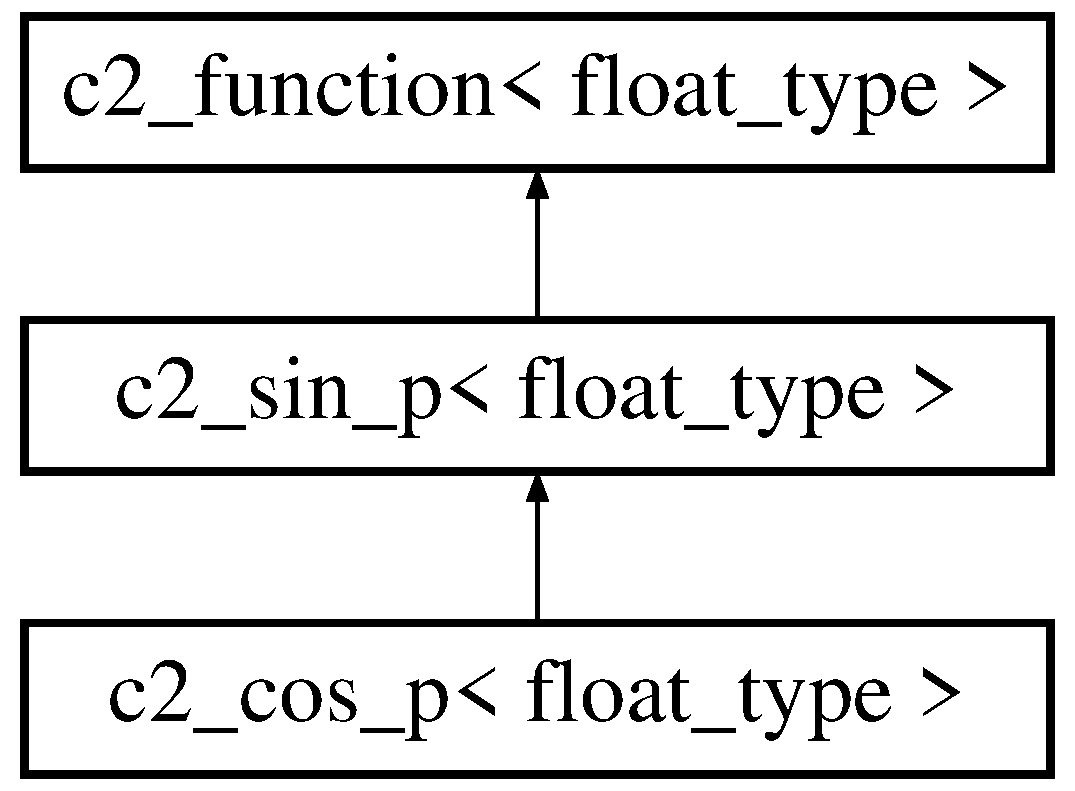
\includegraphics[height=3.000000cm]{classc2__cos__p}
\end{center}
\end{figure}
\subsection*{Public Member Functions}
\begin{DoxyCompactItemize}
\item 
\hypertarget{classc2__cos__p_a407476ff0daa92ac2267e754b74ae133}{\hyperlink{classc2__cos__p_a407476ff0daa92ac2267e754b74ae133}{c2\-\_\-cos\-\_\-p} ()}\label{classc2__cos__p_a407476ff0daa92ac2267e754b74ae133}

\begin{DoxyCompactList}\small\item\em constructor. \end{DoxyCompactList}\item 
virtual float\-\_\-type \hyperlink{classc2__cos__p_ae4e275f2739d33bfbf1f2efc741535d5}{value\-\_\-with\-\_\-derivatives} (float\-\_\-type x, float\-\_\-type $\ast$yprime, float\-\_\-type $\ast$yprime2) const   throw (c2\-\_\-exception)
\begin{DoxyCompactList}\small\item\em get the value and derivatives. \end{DoxyCompactList}\end{DoxyCompactItemize}
\subsection*{Additional Inherited Members}


\subsection{Detailed Description}
\subsubsection*{template$<$typename float\-\_\-type = double$>$class c2\-\_\-cos\-\_\-p$<$ float\-\_\-type $>$}

compute cos(x) with its derivatives.

The factory function \hyperlink{classc2__factory_abc5ea51417ecef590629a39f7a2227e4}{c2\-\_\-factory\-::cos()} creates $\ast$new \hyperlink{classc2__cos__p}{c2\-\_\-cos\-\_\-p} 

\subsection{Member Function Documentation}
\hypertarget{classc2__cos__p_ae4e275f2739d33bfbf1f2efc741535d5}{\index{c2\-\_\-cos\-\_\-p@{c2\-\_\-cos\-\_\-p}!value\-\_\-with\-\_\-derivatives@{value\-\_\-with\-\_\-derivatives}}
\index{value\-\_\-with\-\_\-derivatives@{value\-\_\-with\-\_\-derivatives}!c2_cos_p@{c2\-\_\-cos\-\_\-p}}
\subsubsection[{value\-\_\-with\-\_\-derivatives}]{\setlength{\rightskip}{0pt plus 5cm}template$<$typename float\-\_\-type  = double$>$ virtual float\-\_\-type {\bf c2\-\_\-cos\-\_\-p}$<$ float\-\_\-type $>$\-::value\-\_\-with\-\_\-derivatives (
\begin{DoxyParamCaption}
\item[{float\-\_\-type}]{x, }
\item[{float\-\_\-type $\ast$}]{yprime, }
\item[{float\-\_\-type $\ast$}]{yprime2}
\end{DoxyParamCaption}
) const throw  {\bf c2\-\_\-exception}) \hspace{0.3cm}{\ttfamily [inline]}, {\ttfamily [virtual]}}}\label{classc2__cos__p_ae4e275f2739d33bfbf1f2efc741535d5}


get the value and derivatives. 

There is required checking for null pointers on the derivatives, and most implementations should operate faster if derivatives are not needed. 
\begin{DoxyParams}[1]{Parameters}
\mbox{\tt in}  & {\em x} & the point at which to evaluate the function \\
\hline
\mbox{\tt out}  & {\em yprime} & the first derivative (if pointer is non-\/null) \\
\hline
\mbox{\tt out}  & {\em yprime2} & the second derivative (if pointer is non-\/null) \\
\hline
\end{DoxyParams}
\begin{DoxyReturn}{Returns}
the value of the function 
\end{DoxyReturn}


Reimplemented from \hyperlink{classc2__sin__p_a9710a5d48360f4c6e1568f1ad849dd7b}{c2\-\_\-sin\-\_\-p$<$ float\-\_\-type $>$}.



The documentation for this class was generated from the following file\-:\begin{DoxyCompactItemize}
\item 
\hyperlink{c2__function_8hh}{c2\-\_\-function.\-hh}\end{DoxyCompactItemize}

\hypertarget{classc2__diff__p}{\section{c2\-\_\-diff\-\_\-p$<$ float\-\_\-type $>$ Class Template Reference}
\label{classc2__diff__p}\index{c2\-\_\-diff\-\_\-p$<$ float\-\_\-type $>$@{c2\-\_\-diff\-\_\-p$<$ float\-\_\-type $>$}}
}


create a \hyperlink{classc2__function}{c2\-\_\-function} which is the difference of two other c2\-\_\-functions.

This should always be constructed using \hyperlink{classc2__function_a4c56a4673e00bfad37143c403a0c94c8}{c2\-\_\-function\-::operator-\/()}  




{\ttfamily \#include $<$c2\-\_\-function.\-hh$>$}

Inheritance diagram for c2\-\_\-diff\-\_\-p$<$ float\-\_\-type $>$\-:\begin{figure}[H]
\begin{center}
\leavevmode
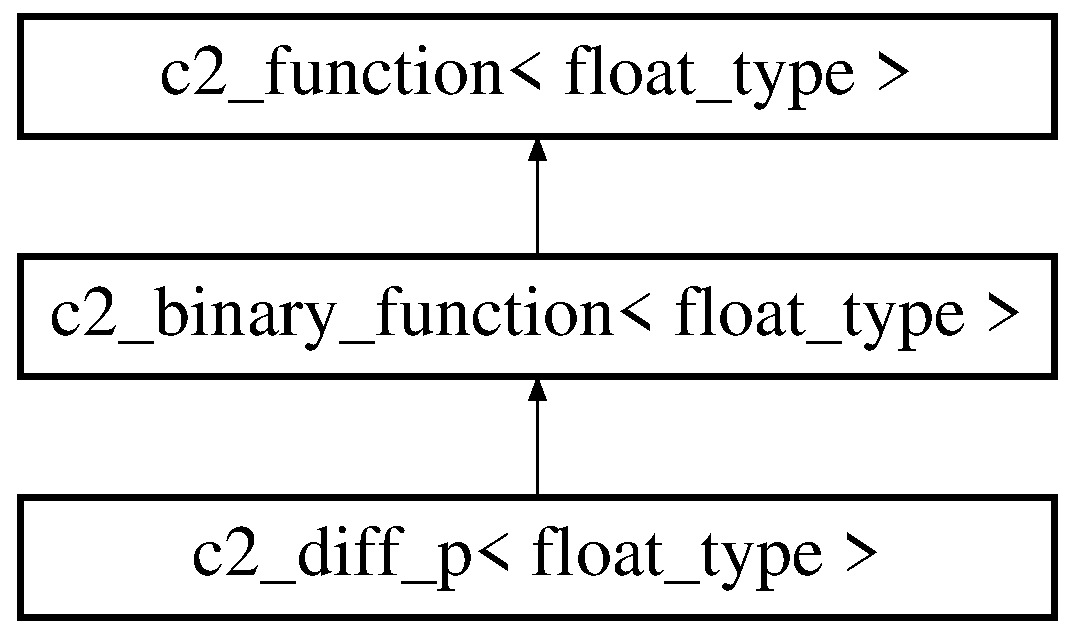
\includegraphics[height=3.000000cm]{classc2__diff__p}
\end{center}
\end{figure}
\subsection*{Public Member Functions}
\begin{DoxyCompactItemize}
\item 
\hyperlink{classc2__diff__p_adcfb42900f8d8712e055171056688818}{c2\-\_\-diff\-\_\-p} (const \hyperlink{classc2__function}{c2\-\_\-function}$<$ float\-\_\-type $>$ \&left, const \hyperlink{classc2__function}{c2\-\_\-function}$<$ float\-\_\-type $>$ \&right)
\begin{DoxyCompactList}\small\item\em construct {\itshape left} -\/ {\itshape right} \end{DoxyCompactList}\item 
\hypertarget{classc2__diff__p_a8e3593f3c2bcdceb79f57461e099db08}{\hyperlink{classc2__diff__p_a8e3593f3c2bcdceb79f57461e099db08}{c2\-\_\-diff\-\_\-p} ()}\label{classc2__diff__p_a8e3593f3c2bcdceb79f57461e099db08}

\begin{DoxyCompactList}\small\item\em Create a stub just for the combiner to avoid statics. \end{DoxyCompactList}\end{DoxyCompactItemize}
\subsection*{Static Public Member Functions}
\begin{DoxyCompactItemize}
\item 
\hypertarget{classc2__diff__p_ae6481f9c5fa1c245fd7c2ef5df096399}{static float\-\_\-type \hyperlink{classc2__diff__p_ae6481f9c5fa1c245fd7c2ef5df096399}{combine} (const \hyperlink{classc2__function}{c2\-\_\-function}$<$ float\-\_\-type $>$ \&left, const \hyperlink{classc2__function}{c2\-\_\-function}$<$ float\-\_\-type $>$ \&right, float\-\_\-type x, float\-\_\-type $\ast$yprime, float\-\_\-type $\ast$yprime2)  throw (c2\-\_\-exception)}\label{classc2__diff__p_ae6481f9c5fa1c245fd7c2ef5df096399}

\begin{DoxyCompactList}\small\item\em execute math necessary to do subtraction \end{DoxyCompactList}\end{DoxyCompactItemize}
\subsection*{Additional Inherited Members}


\subsection{Detailed Description}
\subsubsection*{template$<$typename float\-\_\-type$>$class c2\-\_\-diff\-\_\-p$<$ float\-\_\-type $>$}

create a \hyperlink{classc2__function}{c2\-\_\-function} which is the difference of two other c2\-\_\-functions.

This should always be constructed using \hyperlink{classc2__function_a4c56a4673e00bfad37143c403a0c94c8}{c2\-\_\-function\-::operator-\/()} 

\subsection{Constructor \& Destructor Documentation}
\hypertarget{classc2__diff__p_adcfb42900f8d8712e055171056688818}{\index{c2\-\_\-diff\-\_\-p@{c2\-\_\-diff\-\_\-p}!c2\-\_\-diff\-\_\-p@{c2\-\_\-diff\-\_\-p}}
\index{c2\-\_\-diff\-\_\-p@{c2\-\_\-diff\-\_\-p}!c2_diff_p@{c2\-\_\-diff\-\_\-p}}
\subsubsection[{c2\-\_\-diff\-\_\-p}]{\setlength{\rightskip}{0pt plus 5cm}template$<$typename float\-\_\-type $>$ {\bf c2\-\_\-diff\-\_\-p}$<$ float\-\_\-type $>$\-::{\bf c2\-\_\-diff\-\_\-p} (
\begin{DoxyParamCaption}
\item[{const {\bf c2\-\_\-function}$<$ float\-\_\-type $>$ \&}]{left, }
\item[{const {\bf c2\-\_\-function}$<$ float\-\_\-type $>$ \&}]{right}
\end{DoxyParamCaption}
)\hspace{0.3cm}{\ttfamily [inline]}}}\label{classc2__diff__p_adcfb42900f8d8712e055171056688818}


construct {\itshape left} -\/ {\itshape right} 


\begin{DoxyParams}{Parameters}
{\em left} & the left function \\
\hline
{\em right} & the right function \\
\hline
\end{DoxyParams}


The documentation for this class was generated from the following file\-:\begin{DoxyCompactItemize}
\item 
\hyperlink{c2__function_8hh}{c2\-\_\-function.\-hh}\end{DoxyCompactItemize}

\hypertarget{classc2__exception}{\section{c2\-\_\-exception Class Reference}
\label{classc2__exception}\index{c2\-\_\-exception@{c2\-\_\-exception}}
}


the exception class for \hyperlink{classc2__function}{c2\-\_\-function} operations.  




{\ttfamily \#include $<$c2\-\_\-function.\-hh$>$}

Inheritance diagram for c2\-\_\-exception\-:\begin{figure}[H]
\begin{center}
\leavevmode
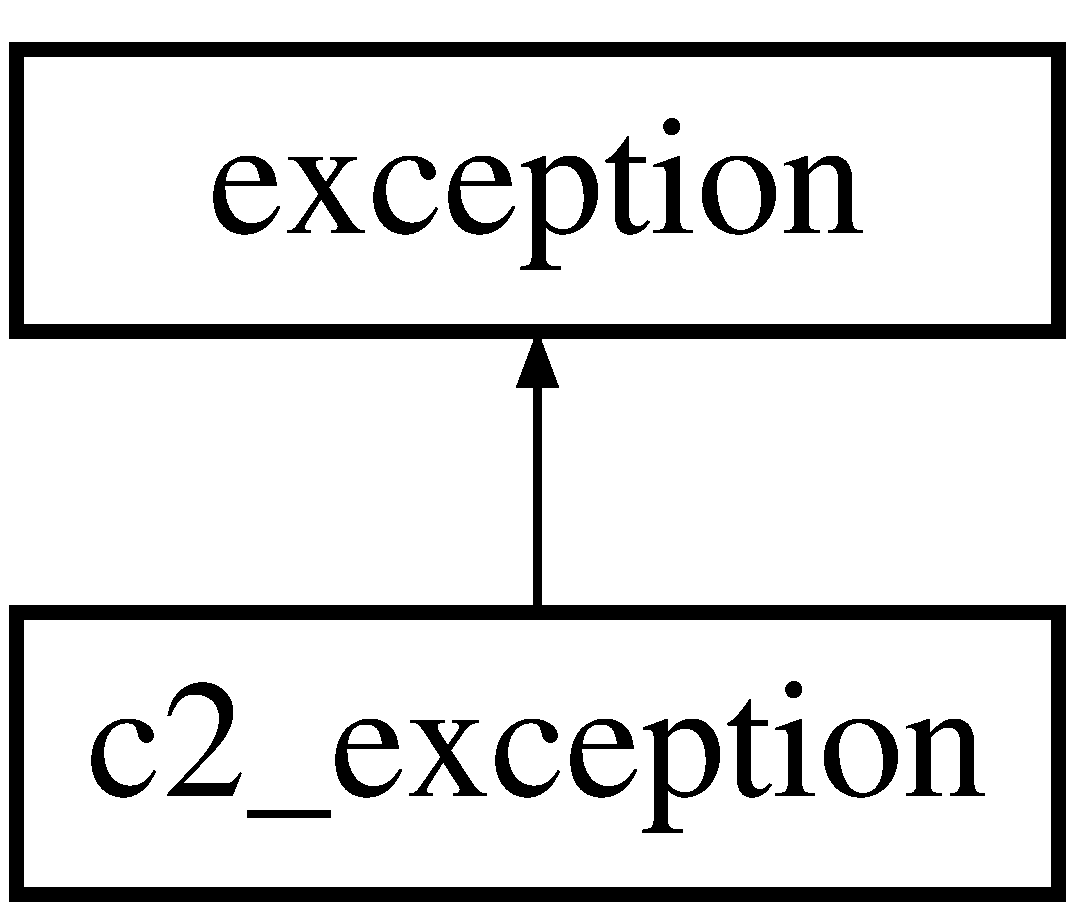
\includegraphics[height=2.000000cm]{classc2__exception}
\end{center}
\end{figure}
\subsection*{Public Member Functions}
\begin{DoxyCompactItemize}
\item 
\hyperlink{classc2__exception_a65e2d283e48111dfa16b7eb92b35c795}{c2\-\_\-exception} (const char msgcode\mbox{[}$\,$\mbox{]})
\begin{DoxyCompactList}\small\item\em construct the exception with an error message \end{DoxyCompactList}\item 
virtual const char $\ast$ \hyperlink{classc2__exception_a5bcb27d5b9f84ecf0410fa387a19c5ef}{what} () const   throw ()
\end{DoxyCompactItemize}


\subsection{Detailed Description}
the exception class for \hyperlink{classc2__function}{c2\-\_\-function} operations. 

\subsection{Constructor \& Destructor Documentation}
\hypertarget{classc2__exception_a65e2d283e48111dfa16b7eb92b35c795}{\index{c2\-\_\-exception@{c2\-\_\-exception}!c2\-\_\-exception@{c2\-\_\-exception}}
\index{c2\-\_\-exception@{c2\-\_\-exception}!c2_exception@{c2\-\_\-exception}}
\subsubsection[{c2\-\_\-exception}]{\setlength{\rightskip}{0pt plus 5cm}c2\-\_\-exception\-::c2\-\_\-exception (
\begin{DoxyParamCaption}
\item[{const char}]{msgcode\mbox{[}$\,$\mbox{]}}
\end{DoxyParamCaption}
)\hspace{0.3cm}{\ttfamily [inline]}}}\label{classc2__exception_a65e2d283e48111dfa16b7eb92b35c795}


construct the exception with an error message 


\begin{DoxyParams}{Parameters}
{\em msgcode} & the message \\
\hline
\end{DoxyParams}


\subsection{Member Function Documentation}
\hypertarget{classc2__exception_a5bcb27d5b9f84ecf0410fa387a19c5ef}{\index{c2\-\_\-exception@{c2\-\_\-exception}!what@{what}}
\index{what@{what}!c2_exception@{c2\-\_\-exception}}
\subsubsection[{what}]{\setlength{\rightskip}{0pt plus 5cm}virtual const char$\ast$ c2\-\_\-exception\-::what (
\begin{DoxyParamCaption}
{}
\end{DoxyParamCaption}
) const throw  ) \hspace{0.3cm}{\ttfamily [inline]}, {\ttfamily [virtual]}}}\label{classc2__exception_a5bcb27d5b9f84ecf0410fa387a19c5ef}
Returns a C-\/style character string describing the general cause of the current error. 

The documentation for this class was generated from the following file\-:\begin{DoxyCompactItemize}
\item 
\hyperlink{c2__function_8hh}{c2\-\_\-function.\-hh}\end{DoxyCompactItemize}

\hypertarget{classc2__exp__p}{\section{c2\-\_\-exp\-\_\-p$<$ float\-\_\-type $>$ Class Template Reference}
\label{classc2__exp__p}\index{c2\-\_\-exp\-\_\-p$<$ float\-\_\-type $>$@{c2\-\_\-exp\-\_\-p$<$ float\-\_\-type $>$}}
}


compute exp(x) with its derivatives.

The factory function \hyperlink{classc2__factory_ad6c29a455b386c1971e6614f6962f3da}{c2\-\_\-factory\-::exp()} creates $\ast$new \hyperlink{classc2__exp__p}{c2\-\_\-exp\-\_\-p}  




{\ttfamily \#include $<$c2\-\_\-function.\-hh$>$}

Inheritance diagram for c2\-\_\-exp\-\_\-p$<$ float\-\_\-type $>$\-:\begin{figure}[H]
\begin{center}
\leavevmode
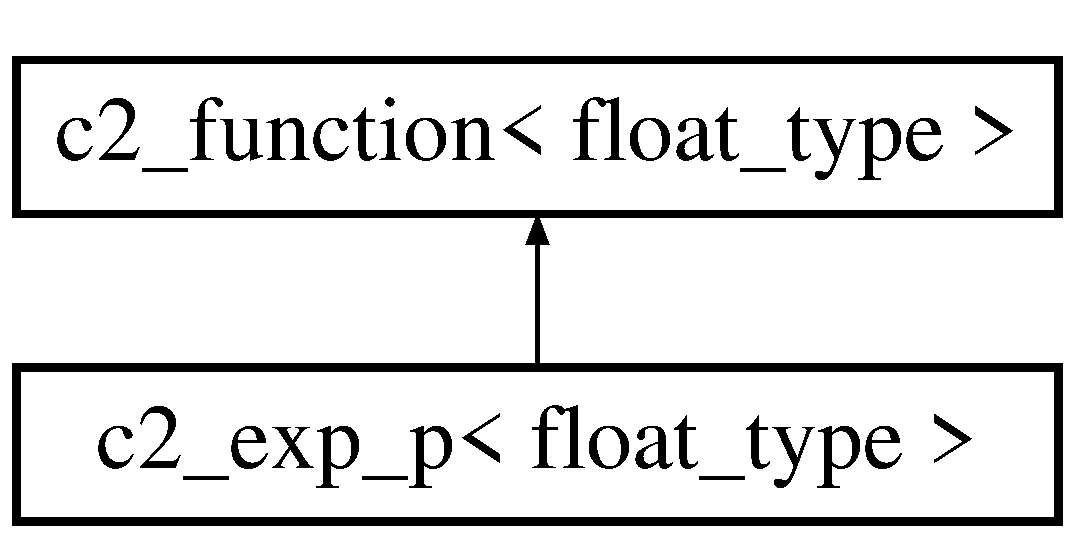
\includegraphics[height=2.000000cm]{classc2__exp__p}
\end{center}
\end{figure}
\subsection*{Public Member Functions}
\begin{DoxyCompactItemize}
\item 
\hypertarget{classc2__exp__p_ae74cc4a62b953936481e8a8bfa265d25}{\hyperlink{classc2__exp__p_ae74cc4a62b953936481e8a8bfa265d25}{c2\-\_\-exp\-\_\-p} ()}\label{classc2__exp__p_ae74cc4a62b953936481e8a8bfa265d25}

\begin{DoxyCompactList}\small\item\em constructor. \end{DoxyCompactList}\item 
virtual float\-\_\-type \hyperlink{classc2__exp__p_a1c5cb28b65356b2f2290ae11d651f93e}{value\-\_\-with\-\_\-derivatives} (float\-\_\-type x, float\-\_\-type $\ast$yprime, float\-\_\-type $\ast$yprime2) const   throw (c2\-\_\-exception)
\begin{DoxyCompactList}\small\item\em get the value and derivatives. \end{DoxyCompactList}\end{DoxyCompactItemize}
\subsection*{Additional Inherited Members}


\subsection{Detailed Description}
\subsubsection*{template$<$typename float\-\_\-type = double$>$class c2\-\_\-exp\-\_\-p$<$ float\-\_\-type $>$}

compute exp(x) with its derivatives.

The factory function \hyperlink{classc2__factory_ad6c29a455b386c1971e6614f6962f3da}{c2\-\_\-factory\-::exp()} creates $\ast$new \hyperlink{classc2__exp__p}{c2\-\_\-exp\-\_\-p} 

\subsection{Member Function Documentation}
\hypertarget{classc2__exp__p_a1c5cb28b65356b2f2290ae11d651f93e}{\index{c2\-\_\-exp\-\_\-p@{c2\-\_\-exp\-\_\-p}!value\-\_\-with\-\_\-derivatives@{value\-\_\-with\-\_\-derivatives}}
\index{value\-\_\-with\-\_\-derivatives@{value\-\_\-with\-\_\-derivatives}!c2_exp_p@{c2\-\_\-exp\-\_\-p}}
\subsubsection[{value\-\_\-with\-\_\-derivatives}]{\setlength{\rightskip}{0pt plus 5cm}template$<$typename float\-\_\-type  = double$>$ virtual float\-\_\-type {\bf c2\-\_\-exp\-\_\-p}$<$ float\-\_\-type $>$\-::value\-\_\-with\-\_\-derivatives (
\begin{DoxyParamCaption}
\item[{float\-\_\-type}]{x, }
\item[{float\-\_\-type $\ast$}]{yprime, }
\item[{float\-\_\-type $\ast$}]{yprime2}
\end{DoxyParamCaption}
) const throw  {\bf c2\-\_\-exception}) \hspace{0.3cm}{\ttfamily [inline]}, {\ttfamily [virtual]}}}\label{classc2__exp__p_a1c5cb28b65356b2f2290ae11d651f93e}


get the value and derivatives. 

There is required checking for null pointers on the derivatives, and most implementations should operate faster if derivatives are not needed. 
\begin{DoxyParams}[1]{Parameters}
\mbox{\tt in}  & {\em x} & the point at which to evaluate the function \\
\hline
\mbox{\tt out}  & {\em yprime} & the first derivative (if pointer is non-\/null) \\
\hline
\mbox{\tt out}  & {\em yprime2} & the second derivative (if pointer is non-\/null) \\
\hline
\end{DoxyParams}
\begin{DoxyReturn}{Returns}
the value of the function 
\end{DoxyReturn}


Implements \hyperlink{classc2__function_a44e0201159111350be7f746fc9026f67}{c2\-\_\-function$<$ float\-\_\-type $>$}.



The documentation for this class was generated from the following file\-:\begin{DoxyCompactItemize}
\item 
\hyperlink{c2__function_8hh}{c2\-\_\-function.\-hh}\end{DoxyCompactItemize}

\hypertarget{classc2__factory}{}\section{c2\+\_\+factory$<$ float\+\_\+type $>$ Class Template Reference}
\label{classc2__factory}\index{c2\+\_\+factory$<$ float\+\_\+type $>$@{c2\+\_\+factory$<$ float\+\_\+type $>$}}


a factory of pre-\/templated \hyperlink{classc2__function}{c2\+\_\+function} generators  




{\ttfamily \#include \char`\"{}c2\+\_\+factory.\+hh\char`\"{}}



Collaboration diagram for c2\+\_\+factory$<$ float\+\_\+type $>$\+:
\nopagebreak
\begin{figure}[H]
\begin{center}
\leavevmode
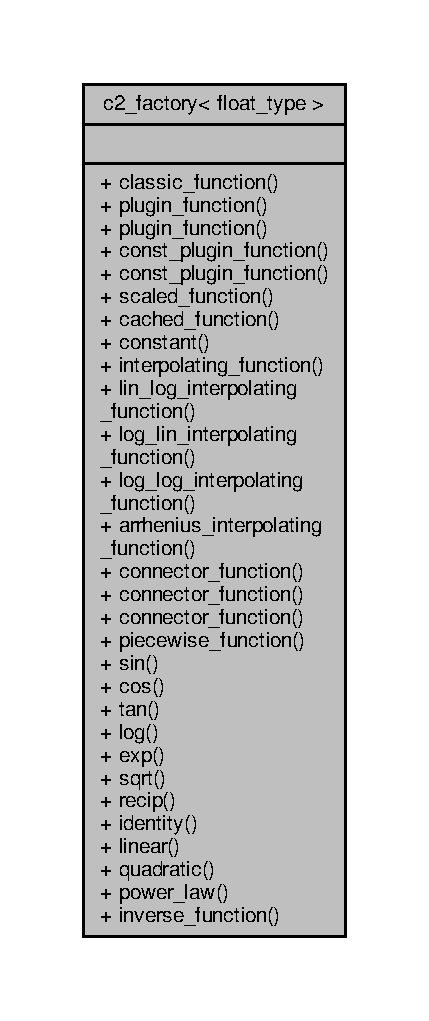
\includegraphics[width=206pt]{classc2__factory__coll__graph}
\end{center}
\end{figure}
\subsection*{Static Public Member Functions}
\begin{DoxyCompactItemize}
\item 
static \hyperlink{classc2__classic__function__p}{c2\+\_\+classic\+\_\+function\+\_\+p}$<$ float\+\_\+type $>$ \& \hyperlink{classc2__factory_ae5c9140b2bfcc6416682562b99479974}{classic\+\_\+function} (float\+\_\+type($\ast$c\+\_\+func)(float\+\_\+type))
\begin{DoxyCompactList}\small\item\em make a $\ast$new object \end{DoxyCompactList}\item 
static \hyperlink{classc2__plugin__function__p}{c2\+\_\+plugin\+\_\+function\+\_\+p}$<$ float\+\_\+type $>$ \& \hyperlink{classc2__factory_aaea82fa4f0b1f0183314a45923a3b673}{plugin\+\_\+function} ()
\begin{DoxyCompactList}\small\item\em make a $\ast$new object \end{DoxyCompactList}\item 
static \hyperlink{classc2__plugin__function__p}{c2\+\_\+plugin\+\_\+function\+\_\+p}$<$ float\+\_\+type $>$ \& \hyperlink{classc2__factory_a1481619ba45f2edb065a6cafc3c8d492}{plugin\+\_\+function} (\hyperlink{classc2__function}{c2\+\_\+function}$<$ float\+\_\+type $>$ \&f)
\begin{DoxyCompactList}\small\item\em make a $\ast$new object \end{DoxyCompactList}\item 
static \hyperlink{classc2__const__plugin__function__p}{c2\+\_\+const\+\_\+plugin\+\_\+function\+\_\+p}$<$ float\+\_\+type $>$ \& \hyperlink{classc2__factory_aebeb20651a347e1fa8f14118faf2588e}{const\+\_\+plugin\+\_\+function} ()
\begin{DoxyCompactList}\small\item\em make a $\ast$new object \end{DoxyCompactList}\item 
static \hyperlink{classc2__const__plugin__function__p}{c2\+\_\+const\+\_\+plugin\+\_\+function\+\_\+p}$<$ float\+\_\+type $>$ \& \hyperlink{classc2__factory_ae377e5df1c8b6eb95b5b02cf8da0667d}{const\+\_\+plugin\+\_\+function} (const \hyperlink{classc2__function}{c2\+\_\+function}$<$ float\+\_\+type $>$ \&f)
\begin{DoxyCompactList}\small\item\em make a $\ast$new object \end{DoxyCompactList}\item 
static \hyperlink{classc2__scaled__function__p}{c2\+\_\+scaled\+\_\+function\+\_\+p}$<$ float\+\_\+type $>$ \& \hyperlink{classc2__factory_a81a7b686b7ffa389ad4dcd8d18997332}{scaled\+\_\+function} (const \hyperlink{classc2__function}{c2\+\_\+function}$<$ float\+\_\+type $>$ \&outer, float\+\_\+type scale)
\begin{DoxyCompactList}\small\item\em make a $\ast$new object \end{DoxyCompactList}\item 
static \hyperlink{classc2__cached__function__p}{c2\+\_\+cached\+\_\+function\+\_\+p}$<$ float\+\_\+type $>$ \& \hyperlink{classc2__factory_aff889f94ad411d97f2e47f1c55fd0324}{cached\+\_\+function} (const \hyperlink{classc2__function}{c2\+\_\+function}$<$ float\+\_\+type $>$ \&func)
\begin{DoxyCompactList}\small\item\em make a $\ast$new object \end{DoxyCompactList}\item 
static \hyperlink{classc2__constant__p}{c2\+\_\+constant\+\_\+p}$<$ float\+\_\+type $>$ \& \hyperlink{classc2__factory_a98e385b2b927d15d4376821302061d4d}{constant} (float\+\_\+type x)
\begin{DoxyCompactList}\small\item\em make a $\ast$new object \end{DoxyCompactList}\item 
static \hyperlink{classinterpolating__function__p}{interpolating\+\_\+function\+\_\+p}$<$ float\+\_\+type $>$ \& \hyperlink{classc2__factory_ab43eaad040801a28019b917c4195b8d5}{interpolating\+\_\+function} ()
\begin{DoxyCompactList}\small\item\em make a $\ast$new object \end{DoxyCompactList}\item 
static \hyperlink{classlin__log__interpolating__function__p}{lin\+\_\+log\+\_\+interpolating\+\_\+function\+\_\+p}$<$ float\+\_\+type $>$ \& \hyperlink{classc2__factory_ab3e9ddf591f0cb2d327dc02c41836232}{lin\+\_\+log\+\_\+interpolating\+\_\+function} ()
\begin{DoxyCompactList}\small\item\em make a $\ast$new object \end{DoxyCompactList}\item 
static \hyperlink{classlog__lin__interpolating__function__p}{log\+\_\+lin\+\_\+interpolating\+\_\+function\+\_\+p}$<$ float\+\_\+type $>$ \& \hyperlink{classc2__factory_afecb73857f9c060b6e32be187705b573}{log\+\_\+lin\+\_\+interpolating\+\_\+function} ()
\begin{DoxyCompactList}\small\item\em make a $\ast$new object \end{DoxyCompactList}\item 
static \hyperlink{classlog__log__interpolating__function__p}{log\+\_\+log\+\_\+interpolating\+\_\+function\+\_\+p}$<$ float\+\_\+type $>$ \& \hyperlink{classc2__factory_a18b0897567e472e50290fcb1834176d3}{log\+\_\+log\+\_\+interpolating\+\_\+function} ()
\begin{DoxyCompactList}\small\item\em make a $\ast$new object \end{DoxyCompactList}\item 
static \hyperlink{classarrhenius__interpolating__function__p}{arrhenius\+\_\+interpolating\+\_\+function\+\_\+p}$<$ float\+\_\+type $>$ \& \hyperlink{classc2__factory_ac2ab3145f84167194ba1ff71aaaa6ffe}{arrhenius\+\_\+interpolating\+\_\+function} ()
\begin{DoxyCompactList}\small\item\em make a $\ast$new object \end{DoxyCompactList}\item 
static \hyperlink{classc2__connector__function__p}{c2\+\_\+connector\+\_\+function\+\_\+p}$<$ float\+\_\+type $>$ \& \hyperlink{classc2__factory_ac8c9d70e5c486a0025e288e5911f2a55}{connector\+\_\+function} (float\+\_\+type x0, const \hyperlink{classc2__function}{c2\+\_\+function}$<$ float\+\_\+type $>$ \&f0, float\+\_\+type x2, const \hyperlink{classc2__function}{c2\+\_\+function}$<$ float\+\_\+type $>$ \&f2, bool auto\+\_\+center, float\+\_\+type y1)
\begin{DoxyCompactList}\small\item\em make a $\ast$new object \end{DoxyCompactList}\item 
static \hyperlink{classc2__connector__function__p}{c2\+\_\+connector\+\_\+function\+\_\+p}$<$ float\+\_\+type $>$ \& \hyperlink{classc2__factory_a6c6d28aecfe189f6eb513ddd8c8a51e1}{connector\+\_\+function} (const \hyperlink{classc2__fblock}{c2\+\_\+fblock}$<$ float\+\_\+type $>$ \&fb0, const \hyperlink{classc2__fblock}{c2\+\_\+fblock}$<$ float\+\_\+type $>$ \&fb2, bool auto\+\_\+center, float\+\_\+type y1)
\begin{DoxyCompactList}\small\item\em make a $\ast$new object \end{DoxyCompactList}\item 
static \hyperlink{classc2__connector__function__p}{c2\+\_\+connector\+\_\+function\+\_\+p}$<$ float\+\_\+type $>$ \& \hyperlink{classc2__factory_a8424d3a67d8e0cbe25f8ad8499da3cd7}{connector\+\_\+function} (float\+\_\+type x0, float\+\_\+type y0, float\+\_\+type yp0, float\+\_\+type ypp0, float\+\_\+type x2, float\+\_\+type y2, float\+\_\+type yp2, float\+\_\+type ypp2, bool auto\+\_\+center, float\+\_\+type y1)
\begin{DoxyCompactList}\small\item\em make a $\ast$new object \end{DoxyCompactList}\item 
static \hyperlink{classc2__piecewise__function__p}{c2\+\_\+piecewise\+\_\+function\+\_\+p}$<$ float\+\_\+type $>$ \& \hyperlink{classc2__factory_ae8073f403ae804870d8ce71e67175507}{piecewise\+\_\+function} ()
\begin{DoxyCompactList}\small\item\em make a $\ast$new object \end{DoxyCompactList}\item 
static \hyperlink{classc2__sin__p}{c2\+\_\+sin\+\_\+p}$<$ float\+\_\+type $>$ \& \hyperlink{classc2__factory_a866854d4fdd6c6678512151dbcd635a5}{sin} ()
\begin{DoxyCompactList}\small\item\em make a $\ast$new object \end{DoxyCompactList}\item 
static \hyperlink{classc2__cos__p}{c2\+\_\+cos\+\_\+p}$<$ float\+\_\+type $>$ \& \hyperlink{classc2__factory_abc5ea51417ecef590629a39f7a2227e4}{cos} ()
\begin{DoxyCompactList}\small\item\em make a $\ast$new object \end{DoxyCompactList}\item 
static \hyperlink{classc2__tan__p}{c2\+\_\+tan\+\_\+p}$<$ float\+\_\+type $>$ \& \hyperlink{classc2__factory_a2f83cbd3be646166f7e3bef1e27244b9}{tan} ()
\begin{DoxyCompactList}\small\item\em make a $\ast$new object \end{DoxyCompactList}\item 
static \hyperlink{classc2__log__p}{c2\+\_\+log\+\_\+p}$<$ float\+\_\+type $>$ \& \hyperlink{classc2__factory_af20c7c4fee421c8ee0b51bac1c42302e}{log} ()
\begin{DoxyCompactList}\small\item\em make a $\ast$new object \end{DoxyCompactList}\item 
static \hyperlink{classc2__exp__p}{c2\+\_\+exp\+\_\+p}$<$ float\+\_\+type $>$ \& \hyperlink{classc2__factory_ad6c29a455b386c1971e6614f6962f3da}{exp} ()
\begin{DoxyCompactList}\small\item\em make a $\ast$new object \end{DoxyCompactList}\item 
static \hyperlink{classc2__sqrt__p}{c2\+\_\+sqrt\+\_\+p}$<$ float\+\_\+type $>$ \& \hyperlink{classc2__factory_a5b189f66ec65267f3812cdc45ccf072d}{sqrt} ()
\begin{DoxyCompactList}\small\item\em make a $\ast$new object \end{DoxyCompactList}\item 
static \hyperlink{classc2__recip__p}{c2\+\_\+recip\+\_\+p}$<$ float\+\_\+type $>$ \& \hyperlink{classc2__factory_adda01279d6b1059843e2aecc5be5d95e}{recip} (float\+\_\+type scale=1)
\begin{DoxyCompactList}\small\item\em make a $\ast$new object \end{DoxyCompactList}\item 
static \hyperlink{classc2__identity__p}{c2\+\_\+identity\+\_\+p}$<$ float\+\_\+type $>$ \& \hyperlink{classc2__factory_a66970667d203c0e63a016b08d2472dc4}{identity} ()
\begin{DoxyCompactList}\small\item\em make a $\ast$new object \end{DoxyCompactList}\item 
static \hyperlink{classc2__linear__p}{c2\+\_\+linear\+\_\+p}$<$ float\+\_\+type $>$ \& \hyperlink{classc2__factory_a2113dc577f24931e0cf316137faf557c}{linear} (float\+\_\+type x0, float\+\_\+type y0, float\+\_\+type slope)
\begin{DoxyCompactList}\small\item\em make a $\ast$new object \end{DoxyCompactList}\item 
static \hyperlink{classc2__quadratic__p}{c2\+\_\+quadratic\+\_\+p}$<$ float\+\_\+type $>$ \& \hyperlink{classc2__factory_a4fb1852ab65ee1c0d62196a260f0df8f}{quadratic} (float\+\_\+type x0, float\+\_\+type y0, float\+\_\+type xcoef, float\+\_\+type x2coef)
\begin{DoxyCompactList}\small\item\em make a $\ast$new object \end{DoxyCompactList}\item 
static \hyperlink{classc2__power__law__p}{c2\+\_\+power\+\_\+law\+\_\+p}$<$ float\+\_\+type $>$ \& \hyperlink{classc2__factory_a2eb1ea80cc3c77555b519108cc0fad6b}{power\+\_\+law} (float\+\_\+type scale, float\+\_\+type power)
\begin{DoxyCompactList}\small\item\em make a $\ast$new object \end{DoxyCompactList}\item 
static \hyperlink{classc2__inverse__function__p}{c2\+\_\+inverse\+\_\+function\+\_\+p}$<$ float\+\_\+type $>$ \& \hyperlink{classc2__factory_aecac3e5856e36ea582da455f1b94c4d7}{inverse\+\_\+function} (const \hyperlink{classc2__function}{c2\+\_\+function}$<$ float\+\_\+type $>$ \&source)
\begin{DoxyCompactList}\small\item\em make a $\ast$new object \end{DoxyCompactList}\end{DoxyCompactItemize}


\subsection{Detailed Description}
\subsubsection*{template$<$typename float\+\_\+type$>$\\*
class c2\+\_\+factory$<$ float\+\_\+type $>$}

a factory of pre-\/templated \hyperlink{classc2__function}{c2\+\_\+function} generators 

do
\begin{DoxyCode}
\textcolor{keyword}{typedef} \hyperlink{classc2__ptr}{c2\_ptr<double>} c2\_p;
\textcolor{keyword}{static} \hyperlink{classc2__factory}{c2\_factory<double>} c2;
c2\_p f=c2.\hyperlink{classc2__factory_a866854d4fdd6c6678512151dbcd635a5}{sin}();
\end{DoxyCode}
 \begin{DoxyNote}{Note}
The factory class doesn\textquotesingle{}t contain any data. It can be statically instantiated at the top of a file, and used everywhere inside, or even instantiated in your project\textquotesingle{}s top-\/level include file. 
\end{DoxyNote}
\begin{DoxySeeAlso}{See also}
c2\+\_\+math\+\_\+factory 
\end{DoxySeeAlso}


\subsection{Member Function Documentation}
\index{c2\+\_\+factory@{c2\+\_\+factory}!arrhenius\+\_\+interpolating\+\_\+function@{arrhenius\+\_\+interpolating\+\_\+function}}
\index{arrhenius\+\_\+interpolating\+\_\+function@{arrhenius\+\_\+interpolating\+\_\+function}!c2\+\_\+factory@{c2\+\_\+factory}}
\subsubsection[{\texorpdfstring{arrhenius\+\_\+interpolating\+\_\+function()}{arrhenius_interpolating_function()}}]{\setlength{\rightskip}{0pt plus 5cm}template$<$typename float\+\_\+type$>$ static {\bf arrhenius\+\_\+interpolating\+\_\+function\+\_\+p}$<$float\+\_\+type$>$\& {\bf c2\+\_\+factory}$<$ float\+\_\+type $>$\+::arrhenius\+\_\+interpolating\+\_\+function (
\begin{DoxyParamCaption}
{}
\end{DoxyParamCaption}
)\hspace{0.3cm}{\ttfamily [inline]}, {\ttfamily [static]}}\hypertarget{classc2__factory_ac2ab3145f84167194ba1ff71aaaa6ffe}{}\label{classc2__factory_ac2ab3145f84167194ba1ff71aaaa6ffe}


make a $\ast$new object 

\index{c2\+\_\+factory@{c2\+\_\+factory}!cached\+\_\+function@{cached\+\_\+function}}
\index{cached\+\_\+function@{cached\+\_\+function}!c2\+\_\+factory@{c2\+\_\+factory}}
\subsubsection[{\texorpdfstring{cached\+\_\+function(const c2\+\_\+function$<$ float\+\_\+type $>$ \&func)}{cached_function(const c2_function< float_type > &func)}}]{\setlength{\rightskip}{0pt plus 5cm}template$<$typename float\+\_\+type$>$ static {\bf c2\+\_\+cached\+\_\+function\+\_\+p}$<$float\+\_\+type$>$\& {\bf c2\+\_\+factory}$<$ float\+\_\+type $>$\+::cached\+\_\+function (
\begin{DoxyParamCaption}
\item[{const {\bf c2\+\_\+function}$<$ float\+\_\+type $>$ \&}]{func}
\end{DoxyParamCaption}
)\hspace{0.3cm}{\ttfamily [inline]}, {\ttfamily [static]}}\hypertarget{classc2__factory_aff889f94ad411d97f2e47f1c55fd0324}{}\label{classc2__factory_aff889f94ad411d97f2e47f1c55fd0324}


make a $\ast$new object 

\index{c2\+\_\+factory@{c2\+\_\+factory}!classic\+\_\+function@{classic\+\_\+function}}
\index{classic\+\_\+function@{classic\+\_\+function}!c2\+\_\+factory@{c2\+\_\+factory}}
\subsubsection[{\texorpdfstring{classic\+\_\+function(float\+\_\+type($\ast$c\+\_\+func)(float\+\_\+type))}{classic_function(float_type(*c_func)(float_type))}}]{\setlength{\rightskip}{0pt plus 5cm}template$<$typename float\+\_\+type$>$ static {\bf c2\+\_\+classic\+\_\+function\+\_\+p}$<$float\+\_\+type$>$\& {\bf c2\+\_\+factory}$<$ float\+\_\+type $>$\+::classic\+\_\+function (
\begin{DoxyParamCaption}
\item[{float\+\_\+type($\ast$)(float\+\_\+type)}]{c\+\_\+func}
\end{DoxyParamCaption}
)\hspace{0.3cm}{\ttfamily [inline]}, {\ttfamily [static]}}\hypertarget{classc2__factory_ae5c9140b2bfcc6416682562b99479974}{}\label{classc2__factory_ae5c9140b2bfcc6416682562b99479974}


make a $\ast$new object 

\index{c2\+\_\+factory@{c2\+\_\+factory}!connector\+\_\+function@{connector\+\_\+function}}
\index{connector\+\_\+function@{connector\+\_\+function}!c2\+\_\+factory@{c2\+\_\+factory}}
\subsubsection[{\texorpdfstring{connector\+\_\+function(float\+\_\+type x0, const c2\+\_\+function$<$ float\+\_\+type $>$ \&f0, float\+\_\+type x2, const c2\+\_\+function$<$ float\+\_\+type $>$ \&f2, bool auto\+\_\+center, float\+\_\+type y1)}{connector_function(float_type x0, const c2_function< float_type > &f0, float_type x2, const c2_function< float_type > &f2, bool auto_center, float_type y1)}}]{\setlength{\rightskip}{0pt plus 5cm}template$<$typename float\+\_\+type$>$ static {\bf c2\+\_\+connector\+\_\+function\+\_\+p}$<$float\+\_\+type$>$\& {\bf c2\+\_\+factory}$<$ float\+\_\+type $>$\+::connector\+\_\+function (
\begin{DoxyParamCaption}
\item[{float\+\_\+type}]{x0, }
\item[{const {\bf c2\+\_\+function}$<$ float\+\_\+type $>$ \&}]{f0, }
\item[{float\+\_\+type}]{x2, }
\item[{const {\bf c2\+\_\+function}$<$ float\+\_\+type $>$ \&}]{f2, }
\item[{bool}]{auto\+\_\+center, }
\item[{float\+\_\+type}]{y1}
\end{DoxyParamCaption}
)\hspace{0.3cm}{\ttfamily [inline]}, {\ttfamily [static]}}\hypertarget{classc2__factory_ac8c9d70e5c486a0025e288e5911f2a55}{}\label{classc2__factory_ac8c9d70e5c486a0025e288e5911f2a55}


make a $\ast$new object 

\index{c2\+\_\+factory@{c2\+\_\+factory}!connector\+\_\+function@{connector\+\_\+function}}
\index{connector\+\_\+function@{connector\+\_\+function}!c2\+\_\+factory@{c2\+\_\+factory}}
\subsubsection[{\texorpdfstring{connector\+\_\+function(const c2\+\_\+fblock$<$ float\+\_\+type $>$ \&fb0, const c2\+\_\+fblock$<$ float\+\_\+type $>$ \&fb2, bool auto\+\_\+center, float\+\_\+type y1)}{connector_function(const c2_fblock< float_type > &fb0, const c2_fblock< float_type > &fb2, bool auto_center, float_type y1)}}]{\setlength{\rightskip}{0pt plus 5cm}template$<$typename float\+\_\+type$>$ static {\bf c2\+\_\+connector\+\_\+function\+\_\+p}$<$float\+\_\+type$>$\& {\bf c2\+\_\+factory}$<$ float\+\_\+type $>$\+::connector\+\_\+function (
\begin{DoxyParamCaption}
\item[{const {\bf c2\+\_\+fblock}$<$ float\+\_\+type $>$ \&}]{fb0, }
\item[{const {\bf c2\+\_\+fblock}$<$ float\+\_\+type $>$ \&}]{fb2, }
\item[{bool}]{auto\+\_\+center, }
\item[{float\+\_\+type}]{y1}
\end{DoxyParamCaption}
)\hspace{0.3cm}{\ttfamily [inline]}, {\ttfamily [static]}}\hypertarget{classc2__factory_a6c6d28aecfe189f6eb513ddd8c8a51e1}{}\label{classc2__factory_a6c6d28aecfe189f6eb513ddd8c8a51e1}


make a $\ast$new object 

\index{c2\+\_\+factory@{c2\+\_\+factory}!connector\+\_\+function@{connector\+\_\+function}}
\index{connector\+\_\+function@{connector\+\_\+function}!c2\+\_\+factory@{c2\+\_\+factory}}
\subsubsection[{\texorpdfstring{connector\+\_\+function(float\+\_\+type x0, float\+\_\+type y0, float\+\_\+type yp0, float\+\_\+type ypp0, float\+\_\+type x2, float\+\_\+type y2, float\+\_\+type yp2, float\+\_\+type ypp2, bool auto\+\_\+center, float\+\_\+type y1)}{connector_function(float_type x0, float_type y0, float_type yp0, float_type ypp0, float_type x2, float_type y2, float_type yp2, float_type ypp2, bool auto_center, float_type y1)}}]{\setlength{\rightskip}{0pt plus 5cm}template$<$typename float\+\_\+type$>$ static {\bf c2\+\_\+connector\+\_\+function\+\_\+p}$<$float\+\_\+type$>$\& {\bf c2\+\_\+factory}$<$ float\+\_\+type $>$\+::connector\+\_\+function (
\begin{DoxyParamCaption}
\item[{float\+\_\+type}]{x0, }
\item[{float\+\_\+type}]{y0, }
\item[{float\+\_\+type}]{yp0, }
\item[{float\+\_\+type}]{ypp0, }
\item[{float\+\_\+type}]{x2, }
\item[{float\+\_\+type}]{y2, }
\item[{float\+\_\+type}]{yp2, }
\item[{float\+\_\+type}]{ypp2, }
\item[{bool}]{auto\+\_\+center, }
\item[{float\+\_\+type}]{y1}
\end{DoxyParamCaption}
)\hspace{0.3cm}{\ttfamily [inline]}, {\ttfamily [static]}}\hypertarget{classc2__factory_a8424d3a67d8e0cbe25f8ad8499da3cd7}{}\label{classc2__factory_a8424d3a67d8e0cbe25f8ad8499da3cd7}


make a $\ast$new object 

\index{c2\+\_\+factory@{c2\+\_\+factory}!const\+\_\+plugin\+\_\+function@{const\+\_\+plugin\+\_\+function}}
\index{const\+\_\+plugin\+\_\+function@{const\+\_\+plugin\+\_\+function}!c2\+\_\+factory@{c2\+\_\+factory}}
\subsubsection[{\texorpdfstring{const\+\_\+plugin\+\_\+function()}{const_plugin_function()}}]{\setlength{\rightskip}{0pt plus 5cm}template$<$typename float\+\_\+type$>$ static {\bf c2\+\_\+const\+\_\+plugin\+\_\+function\+\_\+p}$<$float\+\_\+type$>$\& {\bf c2\+\_\+factory}$<$ float\+\_\+type $>$\+::const\+\_\+plugin\+\_\+function (
\begin{DoxyParamCaption}
{}
\end{DoxyParamCaption}
)\hspace{0.3cm}{\ttfamily [inline]}, {\ttfamily [static]}}\hypertarget{classc2__factory_aebeb20651a347e1fa8f14118faf2588e}{}\label{classc2__factory_aebeb20651a347e1fa8f14118faf2588e}


make a $\ast$new object 

\index{c2\+\_\+factory@{c2\+\_\+factory}!const\+\_\+plugin\+\_\+function@{const\+\_\+plugin\+\_\+function}}
\index{const\+\_\+plugin\+\_\+function@{const\+\_\+plugin\+\_\+function}!c2\+\_\+factory@{c2\+\_\+factory}}
\subsubsection[{\texorpdfstring{const\+\_\+plugin\+\_\+function(const c2\+\_\+function$<$ float\+\_\+type $>$ \&f)}{const_plugin_function(const c2_function< float_type > &f)}}]{\setlength{\rightskip}{0pt plus 5cm}template$<$typename float\+\_\+type$>$ static {\bf c2\+\_\+const\+\_\+plugin\+\_\+function\+\_\+p}$<$float\+\_\+type$>$\& {\bf c2\+\_\+factory}$<$ float\+\_\+type $>$\+::const\+\_\+plugin\+\_\+function (
\begin{DoxyParamCaption}
\item[{const {\bf c2\+\_\+function}$<$ float\+\_\+type $>$ \&}]{f}
\end{DoxyParamCaption}
)\hspace{0.3cm}{\ttfamily [inline]}, {\ttfamily [static]}}\hypertarget{classc2__factory_ae377e5df1c8b6eb95b5b02cf8da0667d}{}\label{classc2__factory_ae377e5df1c8b6eb95b5b02cf8da0667d}


make a $\ast$new object 

\index{c2\+\_\+factory@{c2\+\_\+factory}!constant@{constant}}
\index{constant@{constant}!c2\+\_\+factory@{c2\+\_\+factory}}
\subsubsection[{\texorpdfstring{constant(float\+\_\+type x)}{constant(float_type x)}}]{\setlength{\rightskip}{0pt plus 5cm}template$<$typename float\+\_\+type$>$ static {\bf c2\+\_\+constant\+\_\+p}$<$float\+\_\+type$>$\& {\bf c2\+\_\+factory}$<$ float\+\_\+type $>$\+::constant (
\begin{DoxyParamCaption}
\item[{float\+\_\+type}]{x}
\end{DoxyParamCaption}
)\hspace{0.3cm}{\ttfamily [inline]}, {\ttfamily [static]}}\hypertarget{classc2__factory_a98e385b2b927d15d4376821302061d4d}{}\label{classc2__factory_a98e385b2b927d15d4376821302061d4d}


make a $\ast$new object 

\index{c2\+\_\+factory@{c2\+\_\+factory}!cos@{cos}}
\index{cos@{cos}!c2\+\_\+factory@{c2\+\_\+factory}}
\subsubsection[{\texorpdfstring{cos()}{cos()}}]{\setlength{\rightskip}{0pt plus 5cm}template$<$typename float\+\_\+type$>$ static {\bf c2\+\_\+cos\+\_\+p}$<$float\+\_\+type$>$\& {\bf c2\+\_\+factory}$<$ float\+\_\+type $>$\+::cos (
\begin{DoxyParamCaption}
{}
\end{DoxyParamCaption}
)\hspace{0.3cm}{\ttfamily [inline]}, {\ttfamily [static]}}\hypertarget{classc2__factory_abc5ea51417ecef590629a39f7a2227e4}{}\label{classc2__factory_abc5ea51417ecef590629a39f7a2227e4}


make a $\ast$new object 

\index{c2\+\_\+factory@{c2\+\_\+factory}!exp@{exp}}
\index{exp@{exp}!c2\+\_\+factory@{c2\+\_\+factory}}
\subsubsection[{\texorpdfstring{exp()}{exp()}}]{\setlength{\rightskip}{0pt plus 5cm}template$<$typename float\+\_\+type$>$ static {\bf c2\+\_\+exp\+\_\+p}$<$float\+\_\+type$>$\& {\bf c2\+\_\+factory}$<$ float\+\_\+type $>$\+::exp (
\begin{DoxyParamCaption}
{}
\end{DoxyParamCaption}
)\hspace{0.3cm}{\ttfamily [inline]}, {\ttfamily [static]}}\hypertarget{classc2__factory_ad6c29a455b386c1971e6614f6962f3da}{}\label{classc2__factory_ad6c29a455b386c1971e6614f6962f3da}


make a $\ast$new object 

\index{c2\+\_\+factory@{c2\+\_\+factory}!identity@{identity}}
\index{identity@{identity}!c2\+\_\+factory@{c2\+\_\+factory}}
\subsubsection[{\texorpdfstring{identity()}{identity()}}]{\setlength{\rightskip}{0pt plus 5cm}template$<$typename float\+\_\+type$>$ static {\bf c2\+\_\+identity\+\_\+p}$<$float\+\_\+type$>$\& {\bf c2\+\_\+factory}$<$ float\+\_\+type $>$\+::identity (
\begin{DoxyParamCaption}
{}
\end{DoxyParamCaption}
)\hspace{0.3cm}{\ttfamily [inline]}, {\ttfamily [static]}}\hypertarget{classc2__factory_a66970667d203c0e63a016b08d2472dc4}{}\label{classc2__factory_a66970667d203c0e63a016b08d2472dc4}


make a $\ast$new object 

\index{c2\+\_\+factory@{c2\+\_\+factory}!interpolating\+\_\+function@{interpolating\+\_\+function}}
\index{interpolating\+\_\+function@{interpolating\+\_\+function}!c2\+\_\+factory@{c2\+\_\+factory}}
\subsubsection[{\texorpdfstring{interpolating\+\_\+function()}{interpolating_function()}}]{\setlength{\rightskip}{0pt plus 5cm}template$<$typename float\+\_\+type$>$ static {\bf interpolating\+\_\+function\+\_\+p}$<$float\+\_\+type$>$\& {\bf c2\+\_\+factory}$<$ float\+\_\+type $>$\+::interpolating\+\_\+function (
\begin{DoxyParamCaption}
{}
\end{DoxyParamCaption}
)\hspace{0.3cm}{\ttfamily [inline]}, {\ttfamily [static]}}\hypertarget{classc2__factory_ab43eaad040801a28019b917c4195b8d5}{}\label{classc2__factory_ab43eaad040801a28019b917c4195b8d5}


make a $\ast$new object 

\index{c2\+\_\+factory@{c2\+\_\+factory}!inverse\+\_\+function@{inverse\+\_\+function}}
\index{inverse\+\_\+function@{inverse\+\_\+function}!c2\+\_\+factory@{c2\+\_\+factory}}
\subsubsection[{\texorpdfstring{inverse\+\_\+function(const c2\+\_\+function$<$ float\+\_\+type $>$ \&source)}{inverse_function(const c2_function< float_type > &source)}}]{\setlength{\rightskip}{0pt plus 5cm}template$<$typename float\+\_\+type$>$ static {\bf c2\+\_\+inverse\+\_\+function\+\_\+p}$<$float\+\_\+type$>$\& {\bf c2\+\_\+factory}$<$ float\+\_\+type $>$\+::inverse\+\_\+function (
\begin{DoxyParamCaption}
\item[{const {\bf c2\+\_\+function}$<$ float\+\_\+type $>$ \&}]{source}
\end{DoxyParamCaption}
)\hspace{0.3cm}{\ttfamily [inline]}, {\ttfamily [static]}}\hypertarget{classc2__factory_aecac3e5856e36ea582da455f1b94c4d7}{}\label{classc2__factory_aecac3e5856e36ea582da455f1b94c4d7}


make a $\ast$new object 

\index{c2\+\_\+factory@{c2\+\_\+factory}!lin\+\_\+log\+\_\+interpolating\+\_\+function@{lin\+\_\+log\+\_\+interpolating\+\_\+function}}
\index{lin\+\_\+log\+\_\+interpolating\+\_\+function@{lin\+\_\+log\+\_\+interpolating\+\_\+function}!c2\+\_\+factory@{c2\+\_\+factory}}
\subsubsection[{\texorpdfstring{lin\+\_\+log\+\_\+interpolating\+\_\+function()}{lin_log_interpolating_function()}}]{\setlength{\rightskip}{0pt plus 5cm}template$<$typename float\+\_\+type$>$ static {\bf lin\+\_\+log\+\_\+interpolating\+\_\+function\+\_\+p}$<$float\+\_\+type$>$\& {\bf c2\+\_\+factory}$<$ float\+\_\+type $>$\+::lin\+\_\+log\+\_\+interpolating\+\_\+function (
\begin{DoxyParamCaption}
{}
\end{DoxyParamCaption}
)\hspace{0.3cm}{\ttfamily [inline]}, {\ttfamily [static]}}\hypertarget{classc2__factory_ab3e9ddf591f0cb2d327dc02c41836232}{}\label{classc2__factory_ab3e9ddf591f0cb2d327dc02c41836232}


make a $\ast$new object 

\index{c2\+\_\+factory@{c2\+\_\+factory}!linear@{linear}}
\index{linear@{linear}!c2\+\_\+factory@{c2\+\_\+factory}}
\subsubsection[{\texorpdfstring{linear(float\+\_\+type x0, float\+\_\+type y0, float\+\_\+type slope)}{linear(float_type x0, float_type y0, float_type slope)}}]{\setlength{\rightskip}{0pt plus 5cm}template$<$typename float\+\_\+type$>$ static {\bf c2\+\_\+linear\+\_\+p}$<$float\+\_\+type$>$\& {\bf c2\+\_\+factory}$<$ float\+\_\+type $>$\+::linear (
\begin{DoxyParamCaption}
\item[{float\+\_\+type}]{x0, }
\item[{float\+\_\+type}]{y0, }
\item[{float\+\_\+type}]{slope}
\end{DoxyParamCaption}
)\hspace{0.3cm}{\ttfamily [inline]}, {\ttfamily [static]}}\hypertarget{classc2__factory_a2113dc577f24931e0cf316137faf557c}{}\label{classc2__factory_a2113dc577f24931e0cf316137faf557c}


make a $\ast$new object 

\index{c2\+\_\+factory@{c2\+\_\+factory}!log@{log}}
\index{log@{log}!c2\+\_\+factory@{c2\+\_\+factory}}
\subsubsection[{\texorpdfstring{log()}{log()}}]{\setlength{\rightskip}{0pt plus 5cm}template$<$typename float\+\_\+type$>$ static {\bf c2\+\_\+log\+\_\+p}$<$float\+\_\+type$>$\& {\bf c2\+\_\+factory}$<$ float\+\_\+type $>$\+::log (
\begin{DoxyParamCaption}
{}
\end{DoxyParamCaption}
)\hspace{0.3cm}{\ttfamily [inline]}, {\ttfamily [static]}}\hypertarget{classc2__factory_af20c7c4fee421c8ee0b51bac1c42302e}{}\label{classc2__factory_af20c7c4fee421c8ee0b51bac1c42302e}


make a $\ast$new object 

\index{c2\+\_\+factory@{c2\+\_\+factory}!log\+\_\+lin\+\_\+interpolating\+\_\+function@{log\+\_\+lin\+\_\+interpolating\+\_\+function}}
\index{log\+\_\+lin\+\_\+interpolating\+\_\+function@{log\+\_\+lin\+\_\+interpolating\+\_\+function}!c2\+\_\+factory@{c2\+\_\+factory}}
\subsubsection[{\texorpdfstring{log\+\_\+lin\+\_\+interpolating\+\_\+function()}{log_lin_interpolating_function()}}]{\setlength{\rightskip}{0pt plus 5cm}template$<$typename float\+\_\+type$>$ static {\bf log\+\_\+lin\+\_\+interpolating\+\_\+function\+\_\+p}$<$float\+\_\+type$>$\& {\bf c2\+\_\+factory}$<$ float\+\_\+type $>$\+::log\+\_\+lin\+\_\+interpolating\+\_\+function (
\begin{DoxyParamCaption}
{}
\end{DoxyParamCaption}
)\hspace{0.3cm}{\ttfamily [inline]}, {\ttfamily [static]}}\hypertarget{classc2__factory_afecb73857f9c060b6e32be187705b573}{}\label{classc2__factory_afecb73857f9c060b6e32be187705b573}


make a $\ast$new object 

\index{c2\+\_\+factory@{c2\+\_\+factory}!log\+\_\+log\+\_\+interpolating\+\_\+function@{log\+\_\+log\+\_\+interpolating\+\_\+function}}
\index{log\+\_\+log\+\_\+interpolating\+\_\+function@{log\+\_\+log\+\_\+interpolating\+\_\+function}!c2\+\_\+factory@{c2\+\_\+factory}}
\subsubsection[{\texorpdfstring{log\+\_\+log\+\_\+interpolating\+\_\+function()}{log_log_interpolating_function()}}]{\setlength{\rightskip}{0pt plus 5cm}template$<$typename float\+\_\+type$>$ static {\bf log\+\_\+log\+\_\+interpolating\+\_\+function\+\_\+p}$<$float\+\_\+type$>$\& {\bf c2\+\_\+factory}$<$ float\+\_\+type $>$\+::log\+\_\+log\+\_\+interpolating\+\_\+function (
\begin{DoxyParamCaption}
{}
\end{DoxyParamCaption}
)\hspace{0.3cm}{\ttfamily [inline]}, {\ttfamily [static]}}\hypertarget{classc2__factory_a18b0897567e472e50290fcb1834176d3}{}\label{classc2__factory_a18b0897567e472e50290fcb1834176d3}


make a $\ast$new object 

\index{c2\+\_\+factory@{c2\+\_\+factory}!piecewise\+\_\+function@{piecewise\+\_\+function}}
\index{piecewise\+\_\+function@{piecewise\+\_\+function}!c2\+\_\+factory@{c2\+\_\+factory}}
\subsubsection[{\texorpdfstring{piecewise\+\_\+function()}{piecewise_function()}}]{\setlength{\rightskip}{0pt plus 5cm}template$<$typename float\+\_\+type$>$ static {\bf c2\+\_\+piecewise\+\_\+function\+\_\+p}$<$float\+\_\+type$>$\& {\bf c2\+\_\+factory}$<$ float\+\_\+type $>$\+::piecewise\+\_\+function (
\begin{DoxyParamCaption}
{}
\end{DoxyParamCaption}
)\hspace{0.3cm}{\ttfamily [inline]}, {\ttfamily [static]}}\hypertarget{classc2__factory_ae8073f403ae804870d8ce71e67175507}{}\label{classc2__factory_ae8073f403ae804870d8ce71e67175507}


make a $\ast$new object 

\index{c2\+\_\+factory@{c2\+\_\+factory}!plugin\+\_\+function@{plugin\+\_\+function}}
\index{plugin\+\_\+function@{plugin\+\_\+function}!c2\+\_\+factory@{c2\+\_\+factory}}
\subsubsection[{\texorpdfstring{plugin\+\_\+function()}{plugin_function()}}]{\setlength{\rightskip}{0pt plus 5cm}template$<$typename float\+\_\+type$>$ static {\bf c2\+\_\+plugin\+\_\+function\+\_\+p}$<$float\+\_\+type$>$\& {\bf c2\+\_\+factory}$<$ float\+\_\+type $>$\+::plugin\+\_\+function (
\begin{DoxyParamCaption}
{}
\end{DoxyParamCaption}
)\hspace{0.3cm}{\ttfamily [inline]}, {\ttfamily [static]}}\hypertarget{classc2__factory_aaea82fa4f0b1f0183314a45923a3b673}{}\label{classc2__factory_aaea82fa4f0b1f0183314a45923a3b673}


make a $\ast$new object 

\index{c2\+\_\+factory@{c2\+\_\+factory}!plugin\+\_\+function@{plugin\+\_\+function}}
\index{plugin\+\_\+function@{plugin\+\_\+function}!c2\+\_\+factory@{c2\+\_\+factory}}
\subsubsection[{\texorpdfstring{plugin\+\_\+function(c2\+\_\+function$<$ float\+\_\+type $>$ \&f)}{plugin_function(c2_function< float_type > &f)}}]{\setlength{\rightskip}{0pt plus 5cm}template$<$typename float\+\_\+type$>$ static {\bf c2\+\_\+plugin\+\_\+function\+\_\+p}$<$float\+\_\+type$>$\& {\bf c2\+\_\+factory}$<$ float\+\_\+type $>$\+::plugin\+\_\+function (
\begin{DoxyParamCaption}
\item[{{\bf c2\+\_\+function}$<$ float\+\_\+type $>$ \&}]{f}
\end{DoxyParamCaption}
)\hspace{0.3cm}{\ttfamily [inline]}, {\ttfamily [static]}}\hypertarget{classc2__factory_a1481619ba45f2edb065a6cafc3c8d492}{}\label{classc2__factory_a1481619ba45f2edb065a6cafc3c8d492}


make a $\ast$new object 

\index{c2\+\_\+factory@{c2\+\_\+factory}!power\+\_\+law@{power\+\_\+law}}
\index{power\+\_\+law@{power\+\_\+law}!c2\+\_\+factory@{c2\+\_\+factory}}
\subsubsection[{\texorpdfstring{power\+\_\+law(float\+\_\+type scale, float\+\_\+type power)}{power_law(float_type scale, float_type power)}}]{\setlength{\rightskip}{0pt plus 5cm}template$<$typename float\+\_\+type$>$ static {\bf c2\+\_\+power\+\_\+law\+\_\+p}$<$float\+\_\+type$>$\& {\bf c2\+\_\+factory}$<$ float\+\_\+type $>$\+::power\+\_\+law (
\begin{DoxyParamCaption}
\item[{float\+\_\+type}]{scale, }
\item[{float\+\_\+type}]{power}
\end{DoxyParamCaption}
)\hspace{0.3cm}{\ttfamily [inline]}, {\ttfamily [static]}}\hypertarget{classc2__factory_a2eb1ea80cc3c77555b519108cc0fad6b}{}\label{classc2__factory_a2eb1ea80cc3c77555b519108cc0fad6b}


make a $\ast$new object 

\index{c2\+\_\+factory@{c2\+\_\+factory}!quadratic@{quadratic}}
\index{quadratic@{quadratic}!c2\+\_\+factory@{c2\+\_\+factory}}
\subsubsection[{\texorpdfstring{quadratic(float\+\_\+type x0, float\+\_\+type y0, float\+\_\+type xcoef, float\+\_\+type x2coef)}{quadratic(float_type x0, float_type y0, float_type xcoef, float_type x2coef)}}]{\setlength{\rightskip}{0pt plus 5cm}template$<$typename float\+\_\+type$>$ static {\bf c2\+\_\+quadratic\+\_\+p}$<$float\+\_\+type$>$\& {\bf c2\+\_\+factory}$<$ float\+\_\+type $>$\+::quadratic (
\begin{DoxyParamCaption}
\item[{float\+\_\+type}]{x0, }
\item[{float\+\_\+type}]{y0, }
\item[{float\+\_\+type}]{xcoef, }
\item[{float\+\_\+type}]{x2coef}
\end{DoxyParamCaption}
)\hspace{0.3cm}{\ttfamily [inline]}, {\ttfamily [static]}}\hypertarget{classc2__factory_a4fb1852ab65ee1c0d62196a260f0df8f}{}\label{classc2__factory_a4fb1852ab65ee1c0d62196a260f0df8f}


make a $\ast$new object 

\index{c2\+\_\+factory@{c2\+\_\+factory}!recip@{recip}}
\index{recip@{recip}!c2\+\_\+factory@{c2\+\_\+factory}}
\subsubsection[{\texorpdfstring{recip(float\+\_\+type scale=1)}{recip(float_type scale=1)}}]{\setlength{\rightskip}{0pt plus 5cm}template$<$typename float\+\_\+type$>$ static {\bf c2\+\_\+recip\+\_\+p}$<$float\+\_\+type$>$\& {\bf c2\+\_\+factory}$<$ float\+\_\+type $>$\+::recip (
\begin{DoxyParamCaption}
\item[{float\+\_\+type}]{scale = {\ttfamily 1}}
\end{DoxyParamCaption}
)\hspace{0.3cm}{\ttfamily [inline]}, {\ttfamily [static]}}\hypertarget{classc2__factory_adda01279d6b1059843e2aecc5be5d95e}{}\label{classc2__factory_adda01279d6b1059843e2aecc5be5d95e}


make a $\ast$new object 

\index{c2\+\_\+factory@{c2\+\_\+factory}!scaled\+\_\+function@{scaled\+\_\+function}}
\index{scaled\+\_\+function@{scaled\+\_\+function}!c2\+\_\+factory@{c2\+\_\+factory}}
\subsubsection[{\texorpdfstring{scaled\+\_\+function(const c2\+\_\+function$<$ float\+\_\+type $>$ \&outer, float\+\_\+type scale)}{scaled_function(const c2_function< float_type > &outer, float_type scale)}}]{\setlength{\rightskip}{0pt plus 5cm}template$<$typename float\+\_\+type$>$ static {\bf c2\+\_\+scaled\+\_\+function\+\_\+p}$<$float\+\_\+type$>$\& {\bf c2\+\_\+factory}$<$ float\+\_\+type $>$\+::scaled\+\_\+function (
\begin{DoxyParamCaption}
\item[{const {\bf c2\+\_\+function}$<$ float\+\_\+type $>$ \&}]{outer, }
\item[{float\+\_\+type}]{scale}
\end{DoxyParamCaption}
)\hspace{0.3cm}{\ttfamily [inline]}, {\ttfamily [static]}}\hypertarget{classc2__factory_a81a7b686b7ffa389ad4dcd8d18997332}{}\label{classc2__factory_a81a7b686b7ffa389ad4dcd8d18997332}


make a $\ast$new object 

\index{c2\+\_\+factory@{c2\+\_\+factory}!sin@{sin}}
\index{sin@{sin}!c2\+\_\+factory@{c2\+\_\+factory}}
\subsubsection[{\texorpdfstring{sin()}{sin()}}]{\setlength{\rightskip}{0pt plus 5cm}template$<$typename float\+\_\+type$>$ static {\bf c2\+\_\+sin\+\_\+p}$<$float\+\_\+type$>$\& {\bf c2\+\_\+factory}$<$ float\+\_\+type $>$\+::sin (
\begin{DoxyParamCaption}
{}
\end{DoxyParamCaption}
)\hspace{0.3cm}{\ttfamily [inline]}, {\ttfamily [static]}}\hypertarget{classc2__factory_a866854d4fdd6c6678512151dbcd635a5}{}\label{classc2__factory_a866854d4fdd6c6678512151dbcd635a5}


make a $\ast$new object 

\index{c2\+\_\+factory@{c2\+\_\+factory}!sqrt@{sqrt}}
\index{sqrt@{sqrt}!c2\+\_\+factory@{c2\+\_\+factory}}
\subsubsection[{\texorpdfstring{sqrt()}{sqrt()}}]{\setlength{\rightskip}{0pt plus 5cm}template$<$typename float\+\_\+type$>$ static {\bf c2\+\_\+sqrt\+\_\+p}$<$float\+\_\+type$>$\& {\bf c2\+\_\+factory}$<$ float\+\_\+type $>$\+::sqrt (
\begin{DoxyParamCaption}
{}
\end{DoxyParamCaption}
)\hspace{0.3cm}{\ttfamily [inline]}, {\ttfamily [static]}}\hypertarget{classc2__factory_a5b189f66ec65267f3812cdc45ccf072d}{}\label{classc2__factory_a5b189f66ec65267f3812cdc45ccf072d}


make a $\ast$new object 

\index{c2\+\_\+factory@{c2\+\_\+factory}!tan@{tan}}
\index{tan@{tan}!c2\+\_\+factory@{c2\+\_\+factory}}
\subsubsection[{\texorpdfstring{tan()}{tan()}}]{\setlength{\rightskip}{0pt plus 5cm}template$<$typename float\+\_\+type$>$ static {\bf c2\+\_\+tan\+\_\+p}$<$float\+\_\+type$>$\& {\bf c2\+\_\+factory}$<$ float\+\_\+type $>$\+::tan (
\begin{DoxyParamCaption}
{}
\end{DoxyParamCaption}
)\hspace{0.3cm}{\ttfamily [inline]}, {\ttfamily [static]}}\hypertarget{classc2__factory_a2f83cbd3be646166f7e3bef1e27244b9}{}\label{classc2__factory_a2f83cbd3be646166f7e3bef1e27244b9}


make a $\ast$new object 



The documentation for this class was generated from the following file\+:\begin{DoxyCompactItemize}
\item 
\hyperlink{c2__factory_8hh}{c2\+\_\+factory.\+hh}\end{DoxyCompactItemize}

\hypertarget{classc2__fblock}{}\section{c2\+\_\+fblock$<$ float\+\_\+type $>$ Class Template Reference}
\label{classc2__fblock}\index{c2\+\_\+fblock$<$ float\+\_\+type $>$@{c2\+\_\+fblock$<$ float\+\_\+type $>$}}


structure used to hold evaluated function data at a point.  




{\ttfamily \#include \char`\"{}c2\+\_\+function.\+hh\char`\"{}}



Collaboration diagram for c2\+\_\+fblock$<$ float\+\_\+type $>$\+:
\nopagebreak
\begin{figure}[H]
\begin{center}
\leavevmode
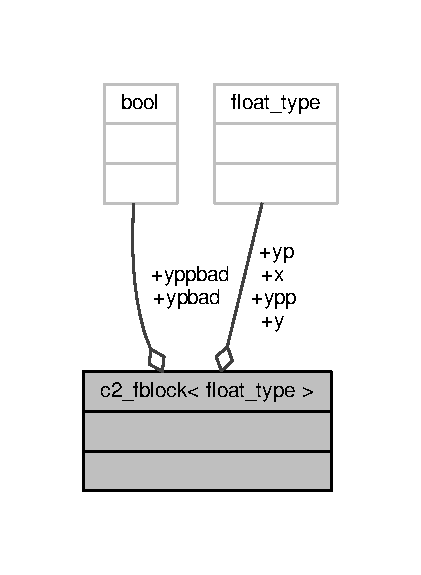
\includegraphics[width=202pt]{classc2__fblock__coll__graph}
\end{center}
\end{figure}
\subsection*{Public Attributes}
\begin{DoxyCompactItemize}
\item 
float\+\_\+type \hyperlink{classc2__fblock_ad5560516bfc794724226af6d3678d518}{x}
\begin{DoxyCompactList}\small\item\em the abscissa \end{DoxyCompactList}\item 
float\+\_\+type \hyperlink{classc2__fblock_a0de289aaf1b624af8cb1461164ea0dfd}{y}
\begin{DoxyCompactList}\small\item\em the value of the function at {\itshape x} \end{DoxyCompactList}\item 
float\+\_\+type \hyperlink{classc2__fblock_a4df4413818bad95cd88e33d29fa7334e}{yp}
\begin{DoxyCompactList}\small\item\em the derivative at {\itshape x} \end{DoxyCompactList}\item 
float\+\_\+type \hyperlink{classc2__fblock_aad33c0adbb2d83549139ab8e9f69c0d3}{ypp}
\begin{DoxyCompactList}\small\item\em the second derivative at {\itshape x} \end{DoxyCompactList}\item 
bool \hyperlink{classc2__fblock_aa75a5d9ec9549d6fa22f6959a101de64}{ypbad}
\begin{DoxyCompactList}\small\item\em flag, filled in by \hyperlink{classc2__function_abdce52d0b89ff5bde13d9390ff8c2ba4}{c2\+\_\+function\+::fill\+\_\+fblock()}, indicating the derivative is NaN of Inf \end{DoxyCompactList}\item 
bool \hyperlink{classc2__fblock_ad07bac2622d2bcfeb7e7892a7db536d3}{yppbad}
\begin{DoxyCompactList}\small\item\em flag, filled in by \hyperlink{classc2__function_abdce52d0b89ff5bde13d9390ff8c2ba4}{c2\+\_\+function\+::fill\+\_\+fblock()}, indicating the second derivative is NaN of Inf \end{DoxyCompactList}\end{DoxyCompactItemize}


\subsection{Detailed Description}
\subsubsection*{template$<$typename float\+\_\+type$>$\\*
class c2\+\_\+fblock$<$ float\+\_\+type $>$}

structure used to hold evaluated function data at a point. 

Contains all the information for the function at one point. 

\subsection{Member Data Documentation}
\index{c2\+\_\+fblock@{c2\+\_\+fblock}!x@{x}}
\index{x@{x}!c2\+\_\+fblock@{c2\+\_\+fblock}}
\subsubsection[{\texorpdfstring{x}{x}}]{\setlength{\rightskip}{0pt plus 5cm}template$<$typename float\+\_\+type$>$ float\+\_\+type {\bf c2\+\_\+fblock}$<$ float\+\_\+type $>$\+::x}\hypertarget{classc2__fblock_ad5560516bfc794724226af6d3678d518}{}\label{classc2__fblock_ad5560516bfc794724226af6d3678d518}


the abscissa 

\index{c2\+\_\+fblock@{c2\+\_\+fblock}!y@{y}}
\index{y@{y}!c2\+\_\+fblock@{c2\+\_\+fblock}}
\subsubsection[{\texorpdfstring{y}{y}}]{\setlength{\rightskip}{0pt plus 5cm}template$<$typename float\+\_\+type$>$ float\+\_\+type {\bf c2\+\_\+fblock}$<$ float\+\_\+type $>$\+::y}\hypertarget{classc2__fblock_a0de289aaf1b624af8cb1461164ea0dfd}{}\label{classc2__fblock_a0de289aaf1b624af8cb1461164ea0dfd}


the value of the function at {\itshape x} 

\index{c2\+\_\+fblock@{c2\+\_\+fblock}!yp@{yp}}
\index{yp@{yp}!c2\+\_\+fblock@{c2\+\_\+fblock}}
\subsubsection[{\texorpdfstring{yp}{yp}}]{\setlength{\rightskip}{0pt plus 5cm}template$<$typename float\+\_\+type$>$ float\+\_\+type {\bf c2\+\_\+fblock}$<$ float\+\_\+type $>$\+::yp}\hypertarget{classc2__fblock_a4df4413818bad95cd88e33d29fa7334e}{}\label{classc2__fblock_a4df4413818bad95cd88e33d29fa7334e}


the derivative at {\itshape x} 

\index{c2\+\_\+fblock@{c2\+\_\+fblock}!ypbad@{ypbad}}
\index{ypbad@{ypbad}!c2\+\_\+fblock@{c2\+\_\+fblock}}
\subsubsection[{\texorpdfstring{ypbad}{ypbad}}]{\setlength{\rightskip}{0pt plus 5cm}template$<$typename float\+\_\+type$>$ bool {\bf c2\+\_\+fblock}$<$ float\+\_\+type $>$\+::ypbad}\hypertarget{classc2__fblock_aa75a5d9ec9549d6fa22f6959a101de64}{}\label{classc2__fblock_aa75a5d9ec9549d6fa22f6959a101de64}


flag, filled in by \hyperlink{classc2__function_abdce52d0b89ff5bde13d9390ff8c2ba4}{c2\+\_\+function\+::fill\+\_\+fblock()}, indicating the derivative is NaN of Inf 

\index{c2\+\_\+fblock@{c2\+\_\+fblock}!ypp@{ypp}}
\index{ypp@{ypp}!c2\+\_\+fblock@{c2\+\_\+fblock}}
\subsubsection[{\texorpdfstring{ypp}{ypp}}]{\setlength{\rightskip}{0pt plus 5cm}template$<$typename float\+\_\+type$>$ float\+\_\+type {\bf c2\+\_\+fblock}$<$ float\+\_\+type $>$\+::ypp}\hypertarget{classc2__fblock_aad33c0adbb2d83549139ab8e9f69c0d3}{}\label{classc2__fblock_aad33c0adbb2d83549139ab8e9f69c0d3}


the second derivative at {\itshape x} 

\index{c2\+\_\+fblock@{c2\+\_\+fblock}!yppbad@{yppbad}}
\index{yppbad@{yppbad}!c2\+\_\+fblock@{c2\+\_\+fblock}}
\subsubsection[{\texorpdfstring{yppbad}{yppbad}}]{\setlength{\rightskip}{0pt plus 5cm}template$<$typename float\+\_\+type$>$ bool {\bf c2\+\_\+fblock}$<$ float\+\_\+type $>$\+::yppbad}\hypertarget{classc2__fblock_ad07bac2622d2bcfeb7e7892a7db536d3}{}\label{classc2__fblock_ad07bac2622d2bcfeb7e7892a7db536d3}


flag, filled in by \hyperlink{classc2__function_abdce52d0b89ff5bde13d9390ff8c2ba4}{c2\+\_\+function\+::fill\+\_\+fblock()}, indicating the second derivative is NaN of Inf 



The documentation for this class was generated from the following file\+:\begin{DoxyCompactItemize}
\item 
\hyperlink{c2__function_8hh}{c2\+\_\+function.\+hh}\end{DoxyCompactItemize}

\hypertarget{classc2__function}{\section{c2\-\_\-function$<$ float\-\_\-type $>$ Class Template Reference}
\label{classc2__function}\index{c2\-\_\-function$<$ float\-\_\-type $>$@{c2\-\_\-function$<$ float\-\_\-type $>$}}
}


the parent class for all c2\-\_\-functions.

c2\-\_\-functions know their value, first, and second derivative at almost every point. They can be efficiently combined with binary operators, via \hyperlink{classc2__binary__function}{c2\-\_\-binary\-\_\-function}, composed via c2\-\_\-composed\-\_\-function\-\_\-, have their roots found via \hyperlink{classc2__function_acd17a7191226578c866d82cb2e9ff89f}{find\-\_\-root()}, and be adaptively integrated via \hyperlink{classc2__function_a89ce5e2f44ebfaf9eb4d66605cde4fde}{partial\-\_\-integrals()} or \hyperlink{classc2__function_a675c5056562332be2e49b38485d322b7}{integral()}. They also can carry information with them about how to find 'interesting' points on the function. This information is set with \hyperlink{classc2__function_a23828c75121b442899ab7a80cf5abbb0}{set\-\_\-sampling\-\_\-grid()} and extracted with \hyperlink{classc2__function_ad03264dcc015e5d0b1b6eb30df3f32be}{get\-\_\-sampling\-\_\-grid()}.  




{\ttfamily \#include $<$c2\-\_\-function.\-hh$>$}

Inheritance diagram for c2\-\_\-function$<$ float\-\_\-type $>$\-:\begin{figure}[H]
\begin{center}
\leavevmode
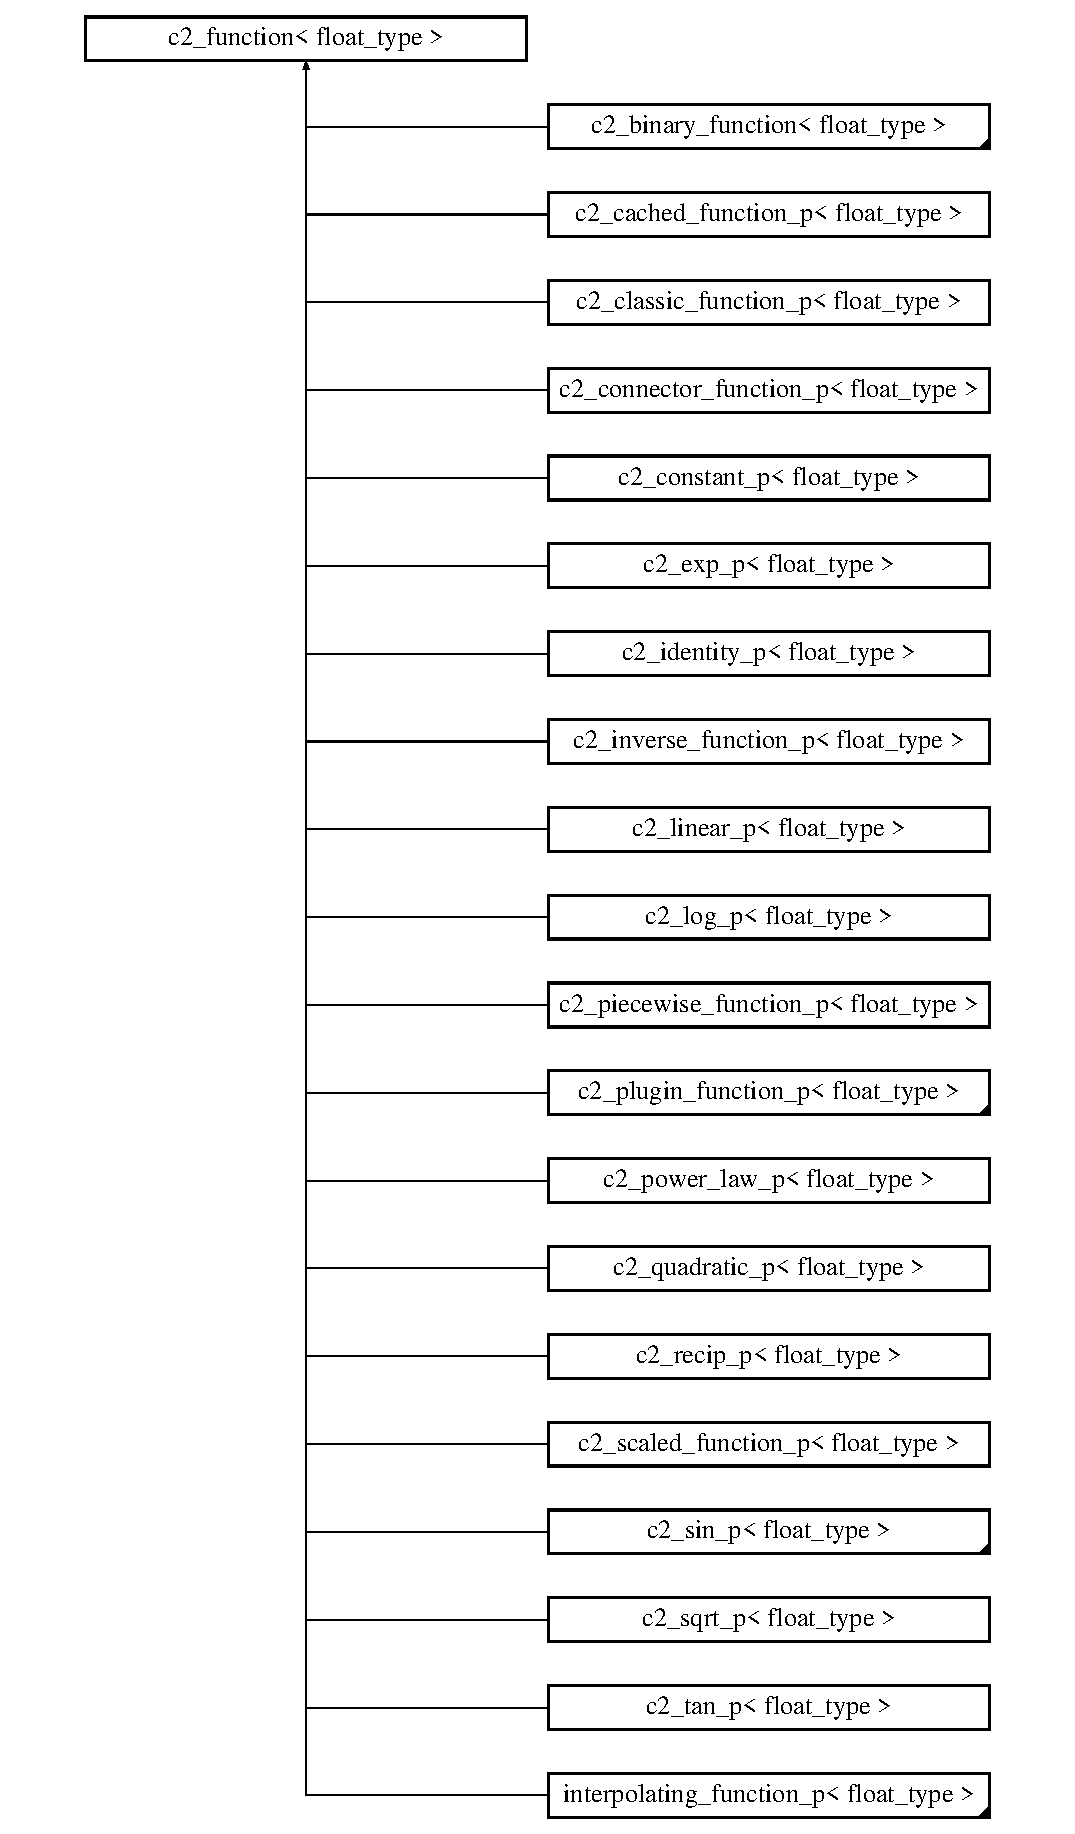
\includegraphics[height=12.000000cm]{classc2__function}
\end{center}
\end{figure}
\subsection*{Public Member Functions}
\begin{DoxyCompactItemize}
\item 
const std\-::string \hyperlink{classc2__function_a851a9e8dca6e8fa9c2da12c8705566b2}{cvs\-\_\-header\-\_\-vers} () const 
\begin{DoxyCompactList}\small\item\em get versioning information for the header file \end{DoxyCompactList}\item 
const std\-::string \hyperlink{classc2__function_a2304b7543724be829571336da02b0f91}{cvs\-\_\-file\-\_\-vers} () const 
\begin{DoxyCompactList}\small\item\em get versioning information for the source file \end{DoxyCompactList}\item 
\hypertarget{classc2__function_ab17870e5af508c66ec154195b837466e}{virtual \hyperlink{classc2__function_ab17870e5af508c66ec154195b837466e}{$\sim$c2\-\_\-function} ()}\label{classc2__function_ab17870e5af508c66ec154195b837466e}

\begin{DoxyCompactList}\small\item\em destructor \end{DoxyCompactList}\item 
virtual float\-\_\-type \hyperlink{classc2__function_a44e0201159111350be7f746fc9026f67}{value\-\_\-with\-\_\-derivatives} (float\-\_\-type x, float\-\_\-type $\ast$yprime, float\-\_\-type $\ast$yprime2) const =0  throw (c2\-\_\-exception)
\begin{DoxyCompactList}\small\item\em get the value and derivatives. \end{DoxyCompactList}\item 
float\-\_\-type \hyperlink{classc2__function_a0658cb22966f0ff9072d4d0e04b54c61}{operator()} (float\-\_\-type x) const   throw (c2\-\_\-exception)
\begin{DoxyCompactList}\small\item\em evaluate the function in the classic way, ignoring derivatives. \end{DoxyCompactList}\item 
float\-\_\-type \hyperlink{classc2__function_a25c89b64e6cbd749314d0a61063240cc}{operator()} (float\-\_\-type x, float\-\_\-type $\ast$yprime, float\-\_\-type $\ast$yprime2) const   throw (c2\-\_\-exception)
\begin{DoxyCompactList}\small\item\em get the value and derivatives. \end{DoxyCompactList}\item 
float\-\_\-type \hyperlink{classc2__function_acd17a7191226578c866d82cb2e9ff89f}{find\-\_\-root} (float\-\_\-type lower\-\_\-bracket, float\-\_\-type upper\-\_\-bracket, float\-\_\-type start, float\-\_\-type value, int $\ast$error=0, float\-\_\-type $\ast$final\-\_\-yprime=0, float\-\_\-type $\ast$final\-\_\-yprime2=0) const   throw (c2\-\_\-exception)
\begin{DoxyCompactList}\small\item\em solve f(x)==value very efficiently, with explicit knowledge of derivatives of the function \end{DoxyCompactList}\item 
float\-\_\-type \hyperlink{classc2__function_a89ce5e2f44ebfaf9eb4d66605cde4fde}{partial\-\_\-integrals} (std\-::vector$<$ float\-\_\-type $>$ xgrid, std\-::vector$<$ float\-\_\-type $>$ $\ast$partials=0, float\-\_\-type abs\-\_\-tol=1e-\/12, float\-\_\-type rel\-\_\-tol=1e-\/12, int derivs=2, bool adapt=true, bool extrapolate=true) const   throw (c2\-\_\-exception)
\begin{DoxyCompactList}\small\item\em for points in xgrid, adaptively return Integral\mbox{[}f(x),\{x,xgrid\mbox{[}i\mbox{]},xgrid\mbox{[}i+1\mbox{]}\}\mbox{]} and return in vector, along with sum \end{DoxyCompactList}\item 
float\-\_\-type \hyperlink{classc2__function_a675c5056562332be2e49b38485d322b7}{integral} (float\-\_\-type amin, float\-\_\-type amax, std\-::vector$<$ float\-\_\-type $>$ $\ast$partials=0, float\-\_\-type abs\-\_\-tol=1e-\/12, float\-\_\-type rel\-\_\-tol=1e-\/12, int derivs=2, bool adapt=true, bool extrapolate=true) const   throw (c2\-\_\-exception)
\begin{DoxyCompactList}\small\item\em a fully-\/automated integrator which uses the information provided by the \hyperlink{classc2__function_ad03264dcc015e5d0b1b6eb30df3f32be}{get\-\_\-sampling\-\_\-grid()} function to figure out what to do. \end{DoxyCompactList}\item 
\hyperlink{classc2__piecewise__function__p}{c2\-\_\-piecewise\-\_\-function\-\_\-p}\\*
$<$ float\-\_\-type $>$ $\ast$ \hyperlink{classc2__function_aea75f73d6a97087571c163ae4e514652}{adaptively\-\_\-sample} (float\-\_\-type amin, float\-\_\-type amax, float\-\_\-type abs\-\_\-tol=1e-\/12, float\-\_\-type rel\-\_\-tol=1e-\/12, int derivs=2, std\-::vector$<$ float\-\_\-type $>$ $\ast$xvals=0, std\-::vector$<$ float\-\_\-type $>$ $\ast$yvals=0) const   throw (c2\-\_\-exception)
\begin{DoxyCompactList}\small\item\em create a \hyperlink{classc2__piecewise__function__p}{c2\-\_\-piecewise\-\_\-function\-\_\-p} from \hyperlink{classc2__connector__function__p}{c2\-\_\-connector\-\_\-function\-\_\-p} segments which is a representation of the parent function to the specified accuracy, but maybe much cheaper to evaluate \end{DoxyCompactList}\item 
\hypertarget{classc2__function_acddff2d033c7f3205658e246d806204b}{float\-\_\-type \hyperlink{classc2__function_acddff2d033c7f3205658e246d806204b}{xmin} () const }\label{classc2__function_acddff2d033c7f3205658e246d806204b}

\begin{DoxyCompactList}\small\item\em return the lower bound of the domain for this function as set by \hyperlink{classc2__function_adeb70da9c75011e9abd71142dca4c22e}{set\-\_\-domain()} \end{DoxyCompactList}\item 
\hypertarget{classc2__function_a7f3ac790b6659b2d137f4c90eadb6ef0}{float\-\_\-type \hyperlink{classc2__function_a7f3ac790b6659b2d137f4c90eadb6ef0}{xmax} () const }\label{classc2__function_a7f3ac790b6659b2d137f4c90eadb6ef0}

\begin{DoxyCompactList}\small\item\em return the upper bound of the domain for this function as set by \hyperlink{classc2__function_adeb70da9c75011e9abd71142dca4c22e}{set\-\_\-domain()} \end{DoxyCompactList}\item 
\hypertarget{classc2__function_adeb70da9c75011e9abd71142dca4c22e}{void \hyperlink{classc2__function_adeb70da9c75011e9abd71142dca4c22e}{set\-\_\-domain} (float\-\_\-type amin, float\-\_\-type amax)}\label{classc2__function_adeb70da9c75011e9abd71142dca4c22e}

\begin{DoxyCompactList}\small\item\em set the domain for this function. \end{DoxyCompactList}\item 
size\-\_\-t \hyperlink{classc2__function_ab6ff0c597019dfb38b1d3d76bfd71e6c}{get\-\_\-evaluations} () const 
\begin{DoxyCompactList}\small\item\em this is a counter owned by the function but which can be used to monitor efficiency of algorithms. \end{DoxyCompactList}\item 
\hypertarget{classc2__function_a8003c40247b7255de5ffbcd3ec21e395}{void \hyperlink{classc2__function_a8003c40247b7255de5ffbcd3ec21e395}{reset\-\_\-evaluations} () const }\label{classc2__function_a8003c40247b7255de5ffbcd3ec21e395}

\begin{DoxyCompactList}\small\item\em reset the counter \end{DoxyCompactList}\item 
\hypertarget{classc2__function_a43555fd6a4ce48f5739e16483170c096}{void \hyperlink{classc2__function_a43555fd6a4ce48f5739e16483170c096}{increment\-\_\-evaluations} () const }\label{classc2__function_a43555fd6a4ce48f5739e16483170c096}

\begin{DoxyCompactList}\small\item\em count evaluations \end{DoxyCompactList}\item 
bool \hyperlink{classc2__function_a8fffb02df5bbff25b0fde67115eae196}{check\-\_\-monotonicity} (const std\-::vector$<$ float\-\_\-type $>$ \&data, const char message\mbox{[}$\,$\mbox{]}) const   throw (c2\-\_\-exception)
\begin{DoxyCompactList}\small\item\em check that a vector is monotonic, throw an exception if not, and return a flag if it is reversed \end{DoxyCompactList}\item 
virtual void \hyperlink{classc2__function_a23828c75121b442899ab7a80cf5abbb0}{set\-\_\-sampling\-\_\-grid} (const std\-::vector$<$ float\-\_\-type $>$ \&grid)  throw (c2\-\_\-exception)
\begin{DoxyCompactList}\small\item\em establish a grid of 'interesting' points on the function. \end{DoxyCompactList}\item 
std\-::vector$<$ float\-\_\-type $>$ $\ast$ \hyperlink{classc2__function_a78b0427521403da116691bab7695906a}{get\-\_\-sampling\-\_\-grid\-\_\-pointer} () const 
\begin{DoxyCompactList}\small\item\em get the sampling grid, which may be a null pointer \end{DoxyCompactList}\item 
virtual void \hyperlink{classc2__function_ad03264dcc015e5d0b1b6eb30df3f32be}{get\-\_\-sampling\-\_\-grid} (float\-\_\-type amin, float\-\_\-type amax, std\-::vector$<$ float\-\_\-type $>$ \&grid) const 
\begin{DoxyCompactList}\small\item\em return the grid of 'interesting' points along this function which lie in the region requested \end{DoxyCompactList}\item 
void \hyperlink{classc2__function_a3f461317f09a62101e6114fd693fa20c}{preen\-\_\-sampling\-\_\-grid} (std\-::vector$<$ float\-\_\-type $>$ $\ast$result) const 
\begin{DoxyCompactList}\small\item\em clean up endpoints on a grid of points \end{DoxyCompactList}\item 
void \hyperlink{classc2__function_a25004cf23f56fafd0b64901354892f3c}{refine\-\_\-sampling\-\_\-grid} (std\-::vector$<$ float\-\_\-type $>$ \&grid, size\-\_\-t refinement) const 
\begin{DoxyCompactList}\small\item\em refine a grid by splitting each interval into more intervals \end{DoxyCompactList}\item 
\hyperlink{classc2__function}{c2\-\_\-function}$<$ float\-\_\-type $>$ \& \hyperlink{classc2__function_ad908929d3a8d8022caf4f3f1c65d5e71}{normalized\-\_\-function} (float\-\_\-type amin, float\-\_\-type amax, float\-\_\-type norm=1.\-0) const   throw (c2\-\_\-exception)
\begin{DoxyCompactList}\small\item\em create a new \hyperlink{classc2__function}{c2\-\_\-function} from this one which is normalized on the interval \end{DoxyCompactList}\item 
\hyperlink{classc2__function}{c2\-\_\-function}$<$ float\-\_\-type $>$ \& \hyperlink{classc2__function_adcf8bcc841ca3a1155ae115178ea88af}{square\-\_\-normalized\-\_\-function} (float\-\_\-type amin, float\-\_\-type amax, float\-\_\-type norm=1.\-0) const   throw (c2\-\_\-exception)
\begin{DoxyCompactList}\small\item\em create a new \hyperlink{classc2__function}{c2\-\_\-function} from this one which is square-\/normalized on the interval \end{DoxyCompactList}\item 
\hyperlink{classc2__function}{c2\-\_\-function}$<$ float\-\_\-type $>$ \& \hyperlink{classc2__function_a9d8716e8abb9e02a188c243f825acf9b}{square\-\_\-normalized\-\_\-function} (float\-\_\-type amin, float\-\_\-type amax, const \hyperlink{classc2__function}{c2\-\_\-function}$<$ float\-\_\-type $>$ \&weight, float\-\_\-type norm=1.\-0) const   throw (c2\-\_\-exception)
\begin{DoxyCompactList}\small\item\em create a new \hyperlink{classc2__function}{c2\-\_\-function} from this one which is square-\/normalized with the provided {\itshape weight} on the interval \end{DoxyCompactList}\item 
\hyperlink{classc2__sum__p}{c2\-\_\-sum\-\_\-p}$<$ float\-\_\-type $>$ \& \hyperlink{classc2__function_a268b206b47c55e635e5f0a9e0f3e8ded}{operator+} (const \hyperlink{classc2__function}{c2\-\_\-function}$<$ float\-\_\-type $>$ \&rhs) const 
\begin{DoxyCompactList}\small\item\em factory function to create a \hyperlink{classc2__sum__p}{c2\-\_\-sum\-\_\-p} from a regular algebraic expression. \end{DoxyCompactList}\item 
\hyperlink{classc2__diff__p}{c2\-\_\-diff\-\_\-p}$<$ float\-\_\-type $>$ \& \hyperlink{classc2__function_a4c56a4673e00bfad37143c403a0c94c8}{operator-\/} (const \hyperlink{classc2__function}{c2\-\_\-function}$<$ float\-\_\-type $>$ \&rhs) const 
\begin{DoxyCompactList}\small\item\em factory function to create a \hyperlink{classc2__diff__p}{c2\-\_\-diff\-\_\-p} from a regular algebraic expression. \end{DoxyCompactList}\item 
\hyperlink{classc2__product__p}{c2\-\_\-product\-\_\-p}$<$ float\-\_\-type $>$ \& \hyperlink{classc2__function_a7744675c98a8ec63320ac1c0b61bec9c}{operator$\ast$} (const \hyperlink{classc2__function}{c2\-\_\-function}$<$ float\-\_\-type $>$ \&rhs) const 
\begin{DoxyCompactList}\small\item\em factory function to create a \hyperlink{classc2__product__p}{c2\-\_\-product\-\_\-p} from a regular algebraic expression. \end{DoxyCompactList}\item 
\hyperlink{classc2__ratio__p}{c2\-\_\-ratio\-\_\-p}$<$ float\-\_\-type $>$ \& \hyperlink{classc2__function_a93ac28dfe5daebea84d147b8e346e60c}{operator/} (const \hyperlink{classc2__function}{c2\-\_\-function}$<$ float\-\_\-type $>$ \&rhs) const 
\begin{DoxyCompactList}\small\item\em factory function to create a \hyperlink{classc2__ratio__p}{c2\-\_\-ratio\-\_\-p} from a regular algebraic expression. \end{DoxyCompactList}\item 
\hyperlink{classc2__composed__function__p}{c2\-\_\-composed\-\_\-function\-\_\-p}\\*
$<$ float\-\_\-type $>$ \& \hyperlink{classc2__function_a9332f7b389579a9b03eb57578649e07f}{operator()} (const \hyperlink{classc2__function}{c2\-\_\-function}$<$ float\-\_\-type $>$ \&inner) const 
\begin{DoxyCompactList}\small\item\em compose this function outside another. \end{DoxyCompactList}\item 
float\-\_\-type \hyperlink{classc2__function_a8e575976851a0b93a9dc2803b4ac2123}{get\-\_\-trouble\-\_\-point} () const 
\begin{DoxyCompactList}\small\item\em Find out where a calculation ran into trouble, if it got a nan. If the most recent computation did not return a nan, this is undefined. \end{DoxyCompactList}\item 
\hypertarget{classc2__function_acd32e22d0b47878dc9fb399a722db61e}{void \hyperlink{classc2__function_acd32e22d0b47878dc9fb399a722db61e}{claim\-\_\-ownership} () const }\label{classc2__function_acd32e22d0b47878dc9fb399a722db61e}

\begin{DoxyCompactList}\small\item\em increment our reference count. Destruction is only legal if the count is zero. \end{DoxyCompactList}\item 
size\-\_\-t \hyperlink{classc2__function_af003b3e29357ccf65b7eba38be877b8c}{release\-\_\-ownership\-\_\-for\-\_\-return} () const   throw (c2\-\_\-exception)
\begin{DoxyCompactList}\small\item\em decrement our reference count. Do not destroy at zero. \end{DoxyCompactList}\item 
\hypertarget{classc2__function_ac98aa40f78c487df141a67174662d749}{void \hyperlink{classc2__function_ac98aa40f78c487df141a67174662d749}{release\-\_\-ownership} () const   throw (c2\-\_\-exception)}\label{classc2__function_ac98aa40f78c487df141a67174662d749}

\begin{DoxyCompactList}\small\item\em decrement our reference count. If the count reaches zero, destroy ourself. \end{DoxyCompactList}\item 
size\-\_\-t \hyperlink{classc2__function_a1df932c78b3521d6a4493972f2642020}{count\-\_\-owners} () const 
\begin{DoxyCompactList}\small\item\em get the reference count, mostly for debugging \end{DoxyCompactList}\item 
void \hyperlink{classc2__function_abdce52d0b89ff5bde13d9390ff8c2ba4}{fill\-\_\-fblock} (\hyperlink{classc2__fblock}{c2\-\_\-fblock}$<$ float\-\_\-type $>$ \&fb) const   throw (c2\-\_\-exception)
\begin{DoxyCompactList}\small\item\em fill in a c2\-\_\-fblock$<$float\-\_\-type$>$... a shortcut for the integrator \& sampler \end{DoxyCompactList}\end{DoxyCompactItemize}
\subsection*{Protected Member Functions}
\begin{DoxyCompactItemize}
\item 
\hypertarget{classc2__function_a0dcc0aa8129ea37e46a72bcafd5d1dc3}{{\bfseries c2\-\_\-function} (const \hyperlink{classc2__function}{c2\-\_\-function}$<$ float\-\_\-type $>$ \&src)}\label{classc2__function_a0dcc0aa8129ea37e46a72bcafd5d1dc3}

\item 
\hypertarget{classc2__function_af06d3b95c044d5ece8343badec919d17}{virtual void {\bfseries set\-\_\-sampling\-\_\-grid\-\_\-pointer} (std\-::vector$<$ float\-\_\-type $>$ \&grid)}\label{classc2__function_af06d3b95c044d5ece8343badec919d17}

\end{DoxyCompactItemize}
\subsection*{Protected Attributes}
\begin{DoxyCompactItemize}
\item 
\hypertarget{classc2__function_ad9714faf2c3d053a77fd733b52834754}{std\-::vector$<$ float\-\_\-type $>$ $\ast$ {\bfseries sampling\-\_\-grid}}\label{classc2__function_ad9714faf2c3d053a77fd733b52834754}

\item 
\hypertarget{classc2__function_a12085ddfc5716c442bb59c5672e140dd}{bool {\bfseries no\-\_\-overwrite\-\_\-grid}}\label{classc2__function_a12085ddfc5716c442bb59c5672e140dd}

\item 
\hypertarget{classc2__function_a72d60216e8a9c61039d4895c6a15b0ce}{float\-\_\-type {\bfseries f\-X\-Min}}\label{classc2__function_a72d60216e8a9c61039d4895c6a15b0ce}

\item 
\hypertarget{classc2__function_a8d000a2d3ca13a119f4bcf4e31a9bca6}{float\-\_\-type {\bfseries f\-X\-Max}}\label{classc2__function_a8d000a2d3ca13a119f4bcf4e31a9bca6}

\item 
\hypertarget{classc2__function_a0737663eb36818cd357852479e6b96f2}{size\-\_\-t {\bfseries evaluations}}\label{classc2__function_a0737663eb36818cd357852479e6b96f2}

\item 
\hypertarget{classc2__function_a19b31dd52b778a2fe5f156def38e41d4}{float\-\_\-type \hyperlink{classc2__function_a19b31dd52b778a2fe5f156def38e41d4}{bad\-\_\-x\-\_\-point}}\label{classc2__function_a19b31dd52b778a2fe5f156def38e41d4}

\begin{DoxyCompactList}\small\item\em this point may be used to record where a calculation ran into trouble \end{DoxyCompactList}\end{DoxyCompactItemize}


\subsection{Detailed Description}
\subsubsection*{template$<$typename float\-\_\-type = double$>$class c2\-\_\-function$<$ float\-\_\-type $>$}

the parent class for all c2\-\_\-functions.

c2\-\_\-functions know their value, first, and second derivative at almost every point. They can be efficiently combined with binary operators, via \hyperlink{classc2__binary__function}{c2\-\_\-binary\-\_\-function}, composed via c2\-\_\-composed\-\_\-function\-\_\-, have their roots found via \hyperlink{classc2__function_acd17a7191226578c866d82cb2e9ff89f}{find\-\_\-root()}, and be adaptively integrated via \hyperlink{classc2__function_a89ce5e2f44ebfaf9eb4d66605cde4fde}{partial\-\_\-integrals()} or \hyperlink{classc2__function_a675c5056562332be2e49b38485d322b7}{integral()}. They also can carry information with them about how to find 'interesting' points on the function. This information is set with \hyperlink{classc2__function_a23828c75121b442899ab7a80cf5abbb0}{set\-\_\-sampling\-\_\-grid()} and extracted with \hyperlink{classc2__function_ad03264dcc015e5d0b1b6eb30df3f32be}{get\-\_\-sampling\-\_\-grid()}. 

Particularly important subclasses are the interpolating functions classes, interpolating\-\_\-function , lin\-\_\-log\-\_\-interpolating\-\_\-function, log\-\_\-lin\-\_\-interpolating\-\_\-function, log\-\_\-log\-\_\-interpolating\-\_\-function, and arrhenius\-\_\-interpolating\-\_\-function, as well as the template functions inverse\-\_\-integrated\-\_\-density\-\_\-function().

For a discussion of memory management, see memory\-\_\-management 

\subsection{Member Function Documentation}
\hypertarget{classc2__function_aea75f73d6a97087571c163ae4e514652}{\index{c2\-\_\-function@{c2\-\_\-function}!adaptively\-\_\-sample@{adaptively\-\_\-sample}}
\index{adaptively\-\_\-sample@{adaptively\-\_\-sample}!c2_function@{c2\-\_\-function}}
\subsubsection[{adaptively\-\_\-sample}]{\setlength{\rightskip}{0pt plus 5cm}template$<$typename float\-\_\-type = double$>$ {\bf c2\-\_\-piecewise\-\_\-function\-\_\-p}$<$float\-\_\-type$>$$\ast$ {\bf c2\-\_\-function}$<$ float\-\_\-type $>$\-::adaptively\-\_\-sample (
\begin{DoxyParamCaption}
\item[{float\-\_\-type}]{amin, }
\item[{float\-\_\-type}]{amax, }
\item[{float\-\_\-type}]{abs\-\_\-tol = {\ttfamily 1e-\/12}, }
\item[{float\-\_\-type}]{rel\-\_\-tol = {\ttfamily 1e-\/12}, }
\item[{int}]{derivs = {\ttfamily 2}, }
\item[{std\-::vector$<$ float\-\_\-type $>$ $\ast$}]{xvals = {\ttfamily 0}, }
\item[{std\-::vector$<$ float\-\_\-type $>$ $\ast$}]{yvals = {\ttfamily 0}}
\end{DoxyParamCaption}
) const throw  {\bf c2\-\_\-exception}) }}\label{classc2__function_aea75f73d6a97087571c163ae4e514652}


create a \hyperlink{classc2__piecewise__function__p}{c2\-\_\-piecewise\-\_\-function\-\_\-p} from \hyperlink{classc2__connector__function__p}{c2\-\_\-connector\-\_\-function\-\_\-p} segments which is a representation of the parent function to the specified accuracy, but maybe much cheaper to evaluate 

This method has three modes, depending on the {\itshape derivs} flag.

If {\itshape derivs} is 2, it computes a \hyperlink{classc2__piecewise__function__p}{c2\-\_\-piecewise\-\_\-function\-\_\-p} representation of its parent function, which may be a much faster function to use in codes if the parent function is expensive. If {\itshape xvals} and {\itshape yvals} are non-\/null, it will also fill them in with the function values at each grid point the adaptive algorithm chooses.

If {\itshape derivs} is 1, this does not create the connectors, and returns an null pointer, but will fill in the {\itshape xvals} and {\itshape yvals} vectors with values of the function at points such that the linear interpolation error between the points is bounded by the tolerance values given. Because it uses derivative information from the function to manage the error control, it is almost completely free of issues with missing periods of oscillatory functions, even with no information provided in the sampling grid. This is typically useful for sampling a function for plotting.

If {\itshape derivs} is 0, this does something very like what it does if {\itshape derivs} = 1, but without derivatives. Instead, to compute the intermediate value of the function for error control, it just uses 3-\/point parabolic interpolation. This is useful amost exclusively for converting a non-\/c2\-\_\-function, with no derivatives, but wrapped in a c2\-\_\-classic\-\_\-function wrapper, into a table of values to seed an \hyperlink{classinterpolating__function__p}{interpolating\-\_\-function\-\_\-p}. Note, however, that without derivatives, this is very susceptible to missing periods of oscillatory functions, so it is important to set a sampling grid which isn't too much coarser than the typical oscillations.

\begin{DoxyNote}{Note}
the {\itshape sampling\-\_\-grid} of the returned function matches the {\itshape sampling\-\_\-grid} of its parent. 
\end{DoxyNote}
\begin{DoxySeeAlso}{See Also}
Adaptive Sampling Examples 
\end{DoxySeeAlso}

\begin{DoxyParams}[1]{Parameters}
 & {\em amin} & lower bound of the domain for sampling \\
\hline
 & {\em amax} & upper bound of the domain for sampling \\
\hline
 & {\em abs\-\_\-tol} & the absolute error bound for each segment \\
\hline
 & {\em rel\-\_\-tol} & the fractional error bound for each segment. \\
\hline
 & {\em derivs} & if 0 or 1, return a useless function, but fill in the {\itshape xvals} and {\itshape yvals} vectors (if non-\/null). Also, if 0 or 1, tolerances refer to linear interpolation, not high-\/order interpolation. If 2, return a full piecewise collection of \hyperlink{classc2__connector__function__p}{c2\-\_\-connector\-\_\-function\-\_\-p} segments. See discussion above. \\
\hline
\mbox{\tt in,out}  & {\em xvals} & vector of abscissas at which the function was actually sampled (if non-\/null) \\
\hline
\mbox{\tt in,out}  & {\em yvals} & vector of function values corresponding to {\itshape xvals} (if non-\/null) \\
\hline
\end{DoxyParams}
\begin{DoxyReturn}{Returns}
a new, sampled representation, if {\itshape derivs} is 2. A null pointer if {\itshape derivs} is 0 or 1. 
\end{DoxyReturn}
\hypertarget{classc2__function_a8fffb02df5bbff25b0fde67115eae196}{\index{c2\-\_\-function@{c2\-\_\-function}!check\-\_\-monotonicity@{check\-\_\-monotonicity}}
\index{check\-\_\-monotonicity@{check\-\_\-monotonicity}!c2_function@{c2\-\_\-function}}
\subsubsection[{check\-\_\-monotonicity}]{\setlength{\rightskip}{0pt plus 5cm}template$<$typename float\-\_\-type = double$>$ bool {\bf c2\-\_\-function}$<$ float\-\_\-type $>$\-::check\-\_\-monotonicity (
\begin{DoxyParamCaption}
\item[{const std\-::vector$<$ float\-\_\-type $>$ \&}]{data, }
\item[{const char}]{message\mbox{[}$\,$\mbox{]}}
\end{DoxyParamCaption}
) const throw  {\bf c2\-\_\-exception}) }}\label{classc2__function_a8fffb02df5bbff25b0fde67115eae196}


check that a vector is monotonic, throw an exception if not, and return a flag if it is reversed 


\begin{DoxyParams}{Parameters}
{\em data} & a vector of data points which are expected to be monotonic. \\
\hline
{\em message} & an informative string to include in an exception if this throws \hyperlink{classc2__exception}{c2\-\_\-exception} \\
\hline
\end{DoxyParams}
\begin{DoxyReturn}{Returns}
true if in decreasing order, false if increasing 
\end{DoxyReturn}
\hypertarget{classc2__function_a1df932c78b3521d6a4493972f2642020}{\index{c2\-\_\-function@{c2\-\_\-function}!count\-\_\-owners@{count\-\_\-owners}}
\index{count\-\_\-owners@{count\-\_\-owners}!c2_function@{c2\-\_\-function}}
\subsubsection[{count\-\_\-owners}]{\setlength{\rightskip}{0pt plus 5cm}template$<$typename float\-\_\-type = double$>$ size\-\_\-t {\bf c2\-\_\-function}$<$ float\-\_\-type $>$\-::count\-\_\-owners (
\begin{DoxyParamCaption}
{}
\end{DoxyParamCaption}
) const\hspace{0.3cm}{\ttfamily [inline]}}}\label{classc2__function_a1df932c78b3521d6a4493972f2642020}


get the reference count, mostly for debugging 

\begin{DoxyReturn}{Returns}
the count 
\end{DoxyReturn}
\hypertarget{classc2__function_a2304b7543724be829571336da02b0f91}{\index{c2\-\_\-function@{c2\-\_\-function}!cvs\-\_\-file\-\_\-vers@{cvs\-\_\-file\-\_\-vers}}
\index{cvs\-\_\-file\-\_\-vers@{cvs\-\_\-file\-\_\-vers}!c2_function@{c2\-\_\-function}}
\subsubsection[{cvs\-\_\-file\-\_\-vers}]{\setlength{\rightskip}{0pt plus 5cm}template$<$typename float\-\_\-type = double$>$ const std\-::string {\bf c2\-\_\-function}$<$ float\-\_\-type $>$\-::cvs\-\_\-file\-\_\-vers (
\begin{DoxyParamCaption}
{}
\end{DoxyParamCaption}
) const}}\label{classc2__function_a2304b7543724be829571336da02b0f91}


get versioning information for the source file 

\begin{DoxyReturn}{Returns}
the C\-V\-S Id string 
\end{DoxyReturn}
\hypertarget{classc2__function_a851a9e8dca6e8fa9c2da12c8705566b2}{\index{c2\-\_\-function@{c2\-\_\-function}!cvs\-\_\-header\-\_\-vers@{cvs\-\_\-header\-\_\-vers}}
\index{cvs\-\_\-header\-\_\-vers@{cvs\-\_\-header\-\_\-vers}!c2_function@{c2\-\_\-function}}
\subsubsection[{cvs\-\_\-header\-\_\-vers}]{\setlength{\rightskip}{0pt plus 5cm}template$<$typename float\-\_\-type = double$>$ const std\-::string {\bf c2\-\_\-function}$<$ float\-\_\-type $>$\-::cvs\-\_\-header\-\_\-vers (
\begin{DoxyParamCaption}
{}
\end{DoxyParamCaption}
) const\hspace{0.3cm}{\ttfamily [inline]}}}\label{classc2__function_a851a9e8dca6e8fa9c2da12c8705566b2}


get versioning information for the header file 

\begin{DoxyReturn}{Returns}
the C\-V\-S Id string 
\end{DoxyReturn}
\hypertarget{classc2__function_abdce52d0b89ff5bde13d9390ff8c2ba4}{\index{c2\-\_\-function@{c2\-\_\-function}!fill\-\_\-fblock@{fill\-\_\-fblock}}
\index{fill\-\_\-fblock@{fill\-\_\-fblock}!c2_function@{c2\-\_\-function}}
\subsubsection[{fill\-\_\-fblock}]{\setlength{\rightskip}{0pt plus 5cm}template$<$typename float\-\_\-type = double$>$ void {\bf c2\-\_\-function}$<$ float\-\_\-type $>$\-::fill\-\_\-fblock (
\begin{DoxyParamCaption}
\item[{{\bf c2\-\_\-fblock}$<$ float\-\_\-type $>$ \&}]{fb}
\end{DoxyParamCaption}
) const throw  {\bf c2\-\_\-exception}) \hspace{0.3cm}{\ttfamily [inline]}}}\label{classc2__function_abdce52d0b89ff5bde13d9390ff8c2ba4}


fill in a c2\-\_\-fblock$<$float\-\_\-type$>$... a shortcut for the integrator \& sampler 


\begin{DoxyParams}[1]{Parameters}
\mbox{\tt in,out}  & {\em fb} & the block to fill in with information \\
\hline
\end{DoxyParams}
\hypertarget{classc2__function_acd17a7191226578c866d82cb2e9ff89f}{\index{c2\-\_\-function@{c2\-\_\-function}!find\-\_\-root@{find\-\_\-root}}
\index{find\-\_\-root@{find\-\_\-root}!c2_function@{c2\-\_\-function}}
\subsubsection[{find\-\_\-root}]{\setlength{\rightskip}{0pt plus 5cm}template$<$typename float\-\_\-type = double$>$ float\-\_\-type {\bf c2\-\_\-function}$<$ float\-\_\-type $>$\-::find\-\_\-root (
\begin{DoxyParamCaption}
\item[{float\-\_\-type}]{lower\-\_\-bracket, }
\item[{float\-\_\-type}]{upper\-\_\-bracket, }
\item[{float\-\_\-type}]{start, }
\item[{float\-\_\-type}]{value, }
\item[{int $\ast$}]{error = {\ttfamily 0}, }
\item[{float\-\_\-type $\ast$}]{final\-\_\-yprime = {\ttfamily 0}, }
\item[{float\-\_\-type $\ast$}]{final\-\_\-yprime2 = {\ttfamily 0}}
\end{DoxyParamCaption}
) const throw  {\bf c2\-\_\-exception}) }}\label{classc2__function_acd17a7191226578c866d82cb2e9ff89f}


solve f(x)==value very efficiently, with explicit knowledge of derivatives of the function 

find\-\_\-root solves by iterated inverse quadratic extrapolation for a solution to f(x)=y. It includes checks against bad convergence, so it should never be able to fail. Unlike typical secant method or fancier Brent's method finders, this does not depend in any strong wasy on the brackets, unless the finder has to resort to successive approximations to close in on a root. Often, it is possible to make the brackets equal to the domain of the function, if there is any clue as to where the root lies, as given by the parameter {\itshape start}. 
\begin{DoxyParams}[1]{Parameters}
 & {\em lower\-\_\-bracket} & the lower bound for the search \\
\hline
 & {\em upper\-\_\-bracket} & the upper bound for the search. Function sign must be opposite to that at {\itshape lower\-\_\-bracket} \\
\hline
 & {\em start} & starting value for the search \\
\hline
 & {\em value} & the value of the function being sought (solves f(x) = {\itshape value}) \\
\hline
\mbox{\tt out}  & {\em error} & If pointer is zero, errors raise exception. Otherwise, returns error here. \\
\hline
\mbox{\tt out}  & {\em final\-\_\-yprime} & If pointer is not zero, return derivative of function at root \\
\hline
\mbox{\tt out}  & {\em final\-\_\-yprime2} & If pointer is not zero, return second derivative of function at root \\
\hline
\end{DoxyParams}
\begin{DoxyReturn}{Returns}
the position of the root. 
\end{DoxyReturn}
\begin{DoxySeeAlso}{See Also}
Root finding sample 
\end{DoxySeeAlso}
\hypertarget{classc2__function_ab6ff0c597019dfb38b1d3d76bfd71e6c}{\index{c2\-\_\-function@{c2\-\_\-function}!get\-\_\-evaluations@{get\-\_\-evaluations}}
\index{get\-\_\-evaluations@{get\-\_\-evaluations}!c2_function@{c2\-\_\-function}}
\subsubsection[{get\-\_\-evaluations}]{\setlength{\rightskip}{0pt plus 5cm}template$<$typename float\-\_\-type = double$>$ size\-\_\-t {\bf c2\-\_\-function}$<$ float\-\_\-type $>$\-::get\-\_\-evaluations (
\begin{DoxyParamCaption}
{}
\end{DoxyParamCaption}
) const\hspace{0.3cm}{\ttfamily [inline]}}}\label{classc2__function_ab6ff0c597019dfb38b1d3d76bfd71e6c}


this is a counter owned by the function but which can be used to monitor efficiency of algorithms. 

It is not maintained automatically in general! The root finder, integrator, and sampler do increment it. \begin{DoxyReturn}{Returns}
number of evaluations logged since last reset. 
\end{DoxyReturn}
\hypertarget{classc2__function_ad03264dcc015e5d0b1b6eb30df3f32be}{\index{c2\-\_\-function@{c2\-\_\-function}!get\-\_\-sampling\-\_\-grid@{get\-\_\-sampling\-\_\-grid}}
\index{get\-\_\-sampling\-\_\-grid@{get\-\_\-sampling\-\_\-grid}!c2_function@{c2\-\_\-function}}
\subsubsection[{get\-\_\-sampling\-\_\-grid}]{\setlength{\rightskip}{0pt plus 5cm}template$<$typename float\-\_\-type = double$>$ virtual void {\bf c2\-\_\-function}$<$ float\-\_\-type $>$\-::get\-\_\-sampling\-\_\-grid (
\begin{DoxyParamCaption}
\item[{float\-\_\-type}]{amin, }
\item[{float\-\_\-type}]{amax, }
\item[{std\-::vector$<$ float\-\_\-type $>$ \&}]{grid}
\end{DoxyParamCaption}
) const\hspace{0.3cm}{\ttfamily [virtual]}}}\label{classc2__function_ad03264dcc015e5d0b1b6eb30df3f32be}


return the grid of 'interesting' points along this function which lie in the region requested 

if a sampling grid is defined, work from there, otherwise return vector of (amin, amax) 
\begin{DoxyParams}[1]{Parameters}
 & {\em amin} & the lower bound for which the function is to be sampled \\
\hline
 & {\em amax} & the upper bound for which the function is to be sampled \\
\hline
\mbox{\tt in,out}  & {\em grid} & filled vector containing the samplng grid. \\
\hline
\end{DoxyParams}


Reimplemented in \hyperlink{classc2__sin__p_a24cee8161741bd4a4dbb24dd782514c1}{c2\-\_\-sin\-\_\-p$<$ float\-\_\-type $>$}, \hyperlink{classc2__plugin__function__p_a0e7ff48329a648b3966efba72b15e3ed}{c2\-\_\-plugin\-\_\-function\-\_\-p$<$ float\-\_\-type $>$}, and \hyperlink{classc2__plugin__function__p_a0e7ff48329a648b3966efba72b15e3ed}{c2\-\_\-plugin\-\_\-function\-\_\-p$<$ G4double $>$}.

\hypertarget{classc2__function_a78b0427521403da116691bab7695906a}{\index{c2\-\_\-function@{c2\-\_\-function}!get\-\_\-sampling\-\_\-grid\-\_\-pointer@{get\-\_\-sampling\-\_\-grid\-\_\-pointer}}
\index{get\-\_\-sampling\-\_\-grid\-\_\-pointer@{get\-\_\-sampling\-\_\-grid\-\_\-pointer}!c2_function@{c2\-\_\-function}}
\subsubsection[{get\-\_\-sampling\-\_\-grid\-\_\-pointer}]{\setlength{\rightskip}{0pt plus 5cm}template$<$typename float\-\_\-type = double$>$ std\-::vector$<$float\-\_\-type$>$$\ast$ {\bf c2\-\_\-function}$<$ float\-\_\-type $>$\-::get\-\_\-sampling\-\_\-grid\-\_\-pointer (
\begin{DoxyParamCaption}
{}
\end{DoxyParamCaption}
) const\hspace{0.3cm}{\ttfamily [inline]}}}\label{classc2__function_a78b0427521403da116691bab7695906a}


get the sampling grid, which may be a null pointer 

\begin{DoxyReturn}{Returns}
pointer to the sampling grid 
\end{DoxyReturn}
\hypertarget{classc2__function_a8e575976851a0b93a9dc2803b4ac2123}{\index{c2\-\_\-function@{c2\-\_\-function}!get\-\_\-trouble\-\_\-point@{get\-\_\-trouble\-\_\-point}}
\index{get\-\_\-trouble\-\_\-point@{get\-\_\-trouble\-\_\-point}!c2_function@{c2\-\_\-function}}
\subsubsection[{get\-\_\-trouble\-\_\-point}]{\setlength{\rightskip}{0pt plus 5cm}template$<$typename float\-\_\-type = double$>$ float\-\_\-type {\bf c2\-\_\-function}$<$ float\-\_\-type $>$\-::get\-\_\-trouble\-\_\-point (
\begin{DoxyParamCaption}
{}
\end{DoxyParamCaption}
) const\hspace{0.3cm}{\ttfamily [inline]}}}\label{classc2__function_a8e575976851a0b93a9dc2803b4ac2123}


Find out where a calculation ran into trouble, if it got a nan. If the most recent computation did not return a nan, this is undefined. 

\begin{DoxyReturn}{Returns}
{\itshape x} value of point at which something went wrong, if integrator (or otherwise) returned a nan. 
\end{DoxyReturn}
\hypertarget{classc2__function_a675c5056562332be2e49b38485d322b7}{\index{c2\-\_\-function@{c2\-\_\-function}!integral@{integral}}
\index{integral@{integral}!c2_function@{c2\-\_\-function}}
\subsubsection[{integral}]{\setlength{\rightskip}{0pt plus 5cm}template$<$typename float\-\_\-type = double$>$ float\-\_\-type {\bf c2\-\_\-function}$<$ float\-\_\-type $>$\-::integral (
\begin{DoxyParamCaption}
\item[{float\-\_\-type}]{amin, }
\item[{float\-\_\-type}]{amax, }
\item[{std\-::vector$<$ float\-\_\-type $>$ $\ast$}]{partials = {\ttfamily 0}, }
\item[{float\-\_\-type}]{abs\-\_\-tol = {\ttfamily 1e-\/12}, }
\item[{float\-\_\-type}]{rel\-\_\-tol = {\ttfamily 1e-\/12}, }
\item[{int}]{derivs = {\ttfamily 2}, }
\item[{bool}]{adapt = {\ttfamily true}, }
\item[{bool}]{extrapolate = {\ttfamily true}}
\end{DoxyParamCaption}
) const throw  {\bf c2\-\_\-exception}) }}\label{classc2__function_a675c5056562332be2e49b38485d322b7}


a fully-\/automated integrator which uses the information provided by the \hyperlink{classc2__function_ad03264dcc015e5d0b1b6eb30df3f32be}{get\-\_\-sampling\-\_\-grid()} function to figure out what to do. 

It returns the integral of the function over the domain requested with error tolerances as specified. It is just a front-\/end to \hyperlink{classc2__function_a89ce5e2f44ebfaf9eb4d66605cde4fde}{partial\-\_\-integrals()}


\begin{DoxyParams}{Parameters}
{\em amin} & lower bound of the domain for integration \\
\hline
{\em amax} & upper bound of the domain for integration \\
\hline
{\em partials} & if non-\/\-N\-U\-L\-L, a vector in which to receive the partial integrals. It will automatically be sized appropriately, if provided, to contain {\itshape n} -\/ 1 elements where {\itshape n} is the length of {\itshape xgrid} \\
\hline
{\em abs\-\_\-tol} & the absolute error bound for each segment \\
\hline
{\em rel\-\_\-tol} & the fractional error bound for each segment. If the error is smaller than either the relative or absolute tolerance, the integration step is finished. \\
\hline
{\em derivs} & number of derivatives to trust, which sets the order of the integrator. The order is 3$\ast${\itshape derivs} + 4. {\itshape derivs} can be 0, 1, or 2. \\
\hline
{\em adapt} & if true, use recursive adaptation, otherwise do simple evaluation on the grid provided with no error checking. \\
\hline
{\em extrapolate} & if true, use simple Richardson extrapolation on the final 2 steps to reduce the error. \\
\hline
\end{DoxyParams}
\begin{DoxyReturn}{Returns}
sum of partial integrals, which is the definite integral from the first value in {\itshape xgrid} to the last. 
\end{DoxyReturn}
\hypertarget{classc2__function_ad908929d3a8d8022caf4f3f1c65d5e71}{\index{c2\-\_\-function@{c2\-\_\-function}!normalized\-\_\-function@{normalized\-\_\-function}}
\index{normalized\-\_\-function@{normalized\-\_\-function}!c2_function@{c2\-\_\-function}}
\subsubsection[{normalized\-\_\-function}]{\setlength{\rightskip}{0pt plus 5cm}template$<$typename float\-\_\-type = double$>$ {\bf c2\-\_\-function}$<$float\-\_\-type$>$\& {\bf c2\-\_\-function}$<$ float\-\_\-type $>$\-::normalized\-\_\-function (
\begin{DoxyParamCaption}
\item[{float\-\_\-type}]{amin, }
\item[{float\-\_\-type}]{amax, }
\item[{float\-\_\-type}]{norm = {\ttfamily 1.0}}
\end{DoxyParamCaption}
) const throw  {\bf c2\-\_\-exception}) }}\label{classc2__function_ad908929d3a8d8022caf4f3f1c65d5e71}


create a new \hyperlink{classc2__function}{c2\-\_\-function} from this one which is normalized on the interval 


\begin{DoxyParams}{Parameters}
{\em amin} & lower bound of the domain for integration \\
\hline
{\em amax} & upper bound of the domain for integration \\
\hline
{\em norm} & the desired integral for the function over the region \\
\hline
\end{DoxyParams}
\begin{DoxyReturn}{Returns}
a new \hyperlink{classc2__function}{c2\-\_\-function} with the desired {\itshape norm}. 
\end{DoxyReturn}
\hypertarget{classc2__function_a0658cb22966f0ff9072d4d0e04b54c61}{\index{c2\-\_\-function@{c2\-\_\-function}!operator()@{operator()}}
\index{operator()@{operator()}!c2_function@{c2\-\_\-function}}
\subsubsection[{operator()}]{\setlength{\rightskip}{0pt plus 5cm}template$<$typename float\-\_\-type = double$>$ float\-\_\-type {\bf c2\-\_\-function}$<$ float\-\_\-type $>$\-::operator() (
\begin{DoxyParamCaption}
\item[{float\-\_\-type}]{x}
\end{DoxyParamCaption}
) const throw  {\bf c2\-\_\-exception}) \hspace{0.3cm}{\ttfamily [inline]}}}\label{classc2__function_a0658cb22966f0ff9072d4d0e04b54c61}


evaluate the function in the classic way, ignoring derivatives. 


\begin{DoxyParams}{Parameters}
{\em x} & the point at which to evaluate \\
\hline
\end{DoxyParams}
\begin{DoxyReturn}{Returns}
the value of the function 
\end{DoxyReturn}
\hypertarget{classc2__function_a25c89b64e6cbd749314d0a61063240cc}{\index{c2\-\_\-function@{c2\-\_\-function}!operator()@{operator()}}
\index{operator()@{operator()}!c2_function@{c2\-\_\-function}}
\subsubsection[{operator()}]{\setlength{\rightskip}{0pt plus 5cm}template$<$typename float\-\_\-type = double$>$ float\-\_\-type {\bf c2\-\_\-function}$<$ float\-\_\-type $>$\-::operator() (
\begin{DoxyParamCaption}
\item[{float\-\_\-type}]{x, }
\item[{float\-\_\-type $\ast$}]{yprime, }
\item[{float\-\_\-type $\ast$}]{yprime2}
\end{DoxyParamCaption}
) const throw  {\bf c2\-\_\-exception}) \hspace{0.3cm}{\ttfamily [inline]}}}\label{classc2__function_a25c89b64e6cbd749314d0a61063240cc}


get the value and derivatives. 


\begin{DoxyParams}[1]{Parameters}
\mbox{\tt in}  & {\em x} & the point at which to evaluate the function \\
\hline
\mbox{\tt out}  & {\em yprime} & the first derivative (if pointer is non-\/null) \\
\hline
\mbox{\tt out}  & {\em yprime2} & the second derivative (if pointer is non-\/null) \\
\hline
\end{DoxyParams}
\begin{DoxyReturn}{Returns}
the value of the function 
\end{DoxyReturn}
\hypertarget{classc2__function_a9332f7b389579a9b03eb57578649e07f}{\index{c2\-\_\-function@{c2\-\_\-function}!operator()@{operator()}}
\index{operator()@{operator()}!c2_function@{c2\-\_\-function}}
\subsubsection[{operator()}]{\setlength{\rightskip}{0pt plus 5cm}template$<$typename float\-\_\-type = double$>$ {\bf c2\-\_\-composed\-\_\-function\-\_\-p}$<$float\-\_\-type$>$\& {\bf c2\-\_\-function}$<$ float\-\_\-type $>$\-::operator() (
\begin{DoxyParamCaption}
\item[{const {\bf c2\-\_\-function}$<$ float\-\_\-type $>$ \&}]{inner}
\end{DoxyParamCaption}
) const\hspace{0.3cm}{\ttfamily [inline]}}}\label{classc2__function_a9332f7b389579a9b03eb57578649e07f}


compose this function outside another. 


\begin{DoxyParams}{Parameters}
{\em inner} & the inner function \\
\hline
\end{DoxyParams}
\begin{DoxyReturn}{Returns}
the composed function \label{classc2__function_compose_operator}%
\hypertarget{classc2__function_compose_operator}{}%
 
\end{DoxyReturn}
\hypertarget{classc2__function_a7744675c98a8ec63320ac1c0b61bec9c}{\index{c2\-\_\-function@{c2\-\_\-function}!operator$\ast$@{operator$\ast$}}
\index{operator$\ast$@{operator$\ast$}!c2_function@{c2\-\_\-function}}
\subsubsection[{operator$\ast$}]{\setlength{\rightskip}{0pt plus 5cm}template$<$typename float\-\_\-type = double$>$ {\bf c2\-\_\-product\-\_\-p}$<$float\-\_\-type$>$\& {\bf c2\-\_\-function}$<$ float\-\_\-type $>$\-::operator$\ast$ (
\begin{DoxyParamCaption}
\item[{const {\bf c2\-\_\-function}$<$ float\-\_\-type $>$ \&}]{rhs}
\end{DoxyParamCaption}
) const\hspace{0.3cm}{\ttfamily [inline]}}}\label{classc2__function_a7744675c98a8ec63320ac1c0b61bec9c}


factory function to create a \hyperlink{classc2__product__p}{c2\-\_\-product\-\_\-p} from a regular algebraic expression. 


\begin{DoxyParams}{Parameters}
{\em rhs} & the right-\/hand term of the product \\
\hline
\end{DoxyParams}
\begin{DoxyReturn}{Returns}
a new \hyperlink{classc2__function}{c2\-\_\-function} 
\end{DoxyReturn}
\hypertarget{classc2__function_a268b206b47c55e635e5f0a9e0f3e8ded}{\index{c2\-\_\-function@{c2\-\_\-function}!operator+@{operator+}}
\index{operator+@{operator+}!c2_function@{c2\-\_\-function}}
\subsubsection[{operator+}]{\setlength{\rightskip}{0pt plus 5cm}template$<$typename float\-\_\-type = double$>$ {\bf c2\-\_\-sum\-\_\-p}$<$float\-\_\-type$>$\& {\bf c2\-\_\-function}$<$ float\-\_\-type $>$\-::operator+ (
\begin{DoxyParamCaption}
\item[{const {\bf c2\-\_\-function}$<$ float\-\_\-type $>$ \&}]{rhs}
\end{DoxyParamCaption}
) const\hspace{0.3cm}{\ttfamily [inline]}}}\label{classc2__function_a268b206b47c55e635e5f0a9e0f3e8ded}


factory function to create a \hyperlink{classc2__sum__p}{c2\-\_\-sum\-\_\-p} from a regular algebraic expression. 


\begin{DoxyParams}{Parameters}
{\em rhs} & the right-\/hand term of the sum \\
\hline
\end{DoxyParams}
\begin{DoxyReturn}{Returns}
a new \hyperlink{classc2__function}{c2\-\_\-function} 
\end{DoxyReturn}
\hypertarget{classc2__function_a4c56a4673e00bfad37143c403a0c94c8}{\index{c2\-\_\-function@{c2\-\_\-function}!operator-\/@{operator-\/}}
\index{operator-\/@{operator-\/}!c2_function@{c2\-\_\-function}}
\subsubsection[{operator-\/}]{\setlength{\rightskip}{0pt plus 5cm}template$<$typename float\-\_\-type = double$>$ {\bf c2\-\_\-diff\-\_\-p}$<$float\-\_\-type$>$\& {\bf c2\-\_\-function}$<$ float\-\_\-type $>$\-::operator-\/ (
\begin{DoxyParamCaption}
\item[{const {\bf c2\-\_\-function}$<$ float\-\_\-type $>$ \&}]{rhs}
\end{DoxyParamCaption}
) const\hspace{0.3cm}{\ttfamily [inline]}}}\label{classc2__function_a4c56a4673e00bfad37143c403a0c94c8}


factory function to create a \hyperlink{classc2__diff__p}{c2\-\_\-diff\-\_\-p} from a regular algebraic expression. 


\begin{DoxyParams}{Parameters}
{\em rhs} & the right-\/hand term of the difference \\
\hline
\end{DoxyParams}
\begin{DoxyReturn}{Returns}
a new \hyperlink{classc2__function}{c2\-\_\-function} 
\end{DoxyReturn}
\hypertarget{classc2__function_a93ac28dfe5daebea84d147b8e346e60c}{\index{c2\-\_\-function@{c2\-\_\-function}!operator/@{operator/}}
\index{operator/@{operator/}!c2_function@{c2\-\_\-function}}
\subsubsection[{operator/}]{\setlength{\rightskip}{0pt plus 5cm}template$<$typename float\-\_\-type = double$>$ {\bf c2\-\_\-ratio\-\_\-p}$<$float\-\_\-type$>$\& {\bf c2\-\_\-function}$<$ float\-\_\-type $>$\-::operator/ (
\begin{DoxyParamCaption}
\item[{const {\bf c2\-\_\-function}$<$ float\-\_\-type $>$ \&}]{rhs}
\end{DoxyParamCaption}
) const\hspace{0.3cm}{\ttfamily [inline]}}}\label{classc2__function_a93ac28dfe5daebea84d147b8e346e60c}


factory function to create a \hyperlink{classc2__ratio__p}{c2\-\_\-ratio\-\_\-p} from a regular algebraic expression. 


\begin{DoxyParams}{Parameters}
{\em rhs} & the right-\/hand term of the ratio (the denominator) \\
\hline
\end{DoxyParams}
\begin{DoxyReturn}{Returns}
a new \hyperlink{classc2__function}{c2\-\_\-function} 
\end{DoxyReturn}
\hypertarget{classc2__function_a89ce5e2f44ebfaf9eb4d66605cde4fde}{\index{c2\-\_\-function@{c2\-\_\-function}!partial\-\_\-integrals@{partial\-\_\-integrals}}
\index{partial\-\_\-integrals@{partial\-\_\-integrals}!c2_function@{c2\-\_\-function}}
\subsubsection[{partial\-\_\-integrals}]{\setlength{\rightskip}{0pt plus 5cm}template$<$typename float\-\_\-type = double$>$ float\-\_\-type {\bf c2\-\_\-function}$<$ float\-\_\-type $>$\-::partial\-\_\-integrals (
\begin{DoxyParamCaption}
\item[{std\-::vector$<$ float\-\_\-type $>$}]{xgrid, }
\item[{std\-::vector$<$ float\-\_\-type $>$ $\ast$}]{partials = {\ttfamily 0}, }
\item[{float\-\_\-type}]{abs\-\_\-tol = {\ttfamily 1e-\/12}, }
\item[{float\-\_\-type}]{rel\-\_\-tol = {\ttfamily 1e-\/12}, }
\item[{int}]{derivs = {\ttfamily 2}, }
\item[{bool}]{adapt = {\ttfamily true}, }
\item[{bool}]{extrapolate = {\ttfamily true}}
\end{DoxyParamCaption}
) const throw  {\bf c2\-\_\-exception}) }}\label{classc2__function_a89ce5e2f44ebfaf9eb4d66605cde4fde}


for points in xgrid, adaptively return Integral\mbox{[}f(x),\{x,xgrid\mbox{[}i\mbox{]},xgrid\mbox{[}i+1\mbox{]}\}\mbox{]} and return in vector, along with sum 

partial\-\_\-integrals uses a method with an error O(dx$\ast$$\ast$10) with full information from the derivatives, and falls back to lower order methods if informed of incomplete derivatives. It uses exact midpoint splitting of the intervals for recursion, resulting in no recomputation of the function during recursive descent at previously computed points. 
\begin{DoxyParams}{Parameters}
{\em xgrid} & points between which to evaluate definite integrals. \\
\hline
{\em partials} & if non-\/\-N\-U\-L\-L, a vector in which to receive the partial integrals. It will automatically be sized apprpropriately, if provided, to contain {\itshape n} -\/ 1 elements where {\itshape n} is the length of {\itshape xgrid} \\
\hline
{\em abs\-\_\-tol} & the absolute error bound for each segment \\
\hline
{\em rel\-\_\-tol} & the fractional error bound for each segment. If the error is smaller than either the relative or absolute tolerance, the integration step is finished. \\
\hline
{\em derivs} & number of derivatives to trust, which sets the order of the integrator. The order is 3$\ast${\itshape derivs} + 4. {\itshape derivs} can be 0, 1, or 2. \\
\hline
{\em adapt} & if true, use recursive adaptation, otherwise do simple evaluation on the grid provided with no error checking. \\
\hline
{\em extrapolate} & if true, use simple Richardson extrapolation on the final 2 steps to reduce the error. \\
\hline
\end{DoxyParams}
\begin{DoxyReturn}{Returns}
sum of partial integrals, which is the definite integral from the first value in {\itshape xgrid} to the last. 
\end{DoxyReturn}
\hypertarget{classc2__function_a3f461317f09a62101e6114fd693fa20c}{\index{c2\-\_\-function@{c2\-\_\-function}!preen\-\_\-sampling\-\_\-grid@{preen\-\_\-sampling\-\_\-grid}}
\index{preen\-\_\-sampling\-\_\-grid@{preen\-\_\-sampling\-\_\-grid}!c2_function@{c2\-\_\-function}}
\subsubsection[{preen\-\_\-sampling\-\_\-grid}]{\setlength{\rightskip}{0pt plus 5cm}template$<$typename float\-\_\-type = double$>$ void {\bf c2\-\_\-function}$<$ float\-\_\-type $>$\-::preen\-\_\-sampling\-\_\-grid (
\begin{DoxyParamCaption}
\item[{std\-::vector$<$ float\-\_\-type $>$ $\ast$}]{result}
\end{DoxyParamCaption}
) const}}\label{classc2__function_a3f461317f09a62101e6114fd693fa20c}


clean up endpoints on a grid of points 


\begin{DoxyParams}[1]{Parameters}
\mbox{\tt in,out}  & {\em result} & the sampling grid with excessively closely space endpoints removed. The grid is modified in place. \\
\hline
\end{DoxyParams}
\hypertarget{classc2__function_a25004cf23f56fafd0b64901354892f3c}{\index{c2\-\_\-function@{c2\-\_\-function}!refine\-\_\-sampling\-\_\-grid@{refine\-\_\-sampling\-\_\-grid}}
\index{refine\-\_\-sampling\-\_\-grid@{refine\-\_\-sampling\-\_\-grid}!c2_function@{c2\-\_\-function}}
\subsubsection[{refine\-\_\-sampling\-\_\-grid}]{\setlength{\rightskip}{0pt plus 5cm}template$<$typename float\-\_\-type = double$>$ void {\bf c2\-\_\-function}$<$ float\-\_\-type $>$\-::refine\-\_\-sampling\-\_\-grid (
\begin{DoxyParamCaption}
\item[{std\-::vector$<$ float\-\_\-type $>$ \&}]{grid, }
\item[{size\-\_\-t}]{refinement}
\end{DoxyParamCaption}
) const}}\label{classc2__function_a25004cf23f56fafd0b64901354892f3c}


refine a grid by splitting each interval into more intervals 


\begin{DoxyParams}[1]{Parameters}
\mbox{\tt in,out}  & {\em grid} & the grid to refine in place \\
\hline
 & {\em refinement} & the number of new steps for each old step \\
\hline
\end{DoxyParams}
\hypertarget{classc2__function_af003b3e29357ccf65b7eba38be877b8c}{\index{c2\-\_\-function@{c2\-\_\-function}!release\-\_\-ownership\-\_\-for\-\_\-return@{release\-\_\-ownership\-\_\-for\-\_\-return}}
\index{release\-\_\-ownership\-\_\-for\-\_\-return@{release\-\_\-ownership\-\_\-for\-\_\-return}!c2_function@{c2\-\_\-function}}
\subsubsection[{release\-\_\-ownership\-\_\-for\-\_\-return}]{\setlength{\rightskip}{0pt plus 5cm}template$<$typename float\-\_\-type = double$>$ size\-\_\-t {\bf c2\-\_\-function}$<$ float\-\_\-type $>$\-::release\-\_\-ownership\-\_\-for\-\_\-return (
\begin{DoxyParamCaption}
{}
\end{DoxyParamCaption}
) const throw  {\bf c2\-\_\-exception}) \hspace{0.3cm}{\ttfamily [inline]}}}\label{classc2__function_af003b3e29357ccf65b7eba38be877b8c}


decrement our reference count. Do not destroy at zero. 

\begin{DoxyReturn}{Returns}
final owner count, to check whether object should disappear. 
\end{DoxyReturn}
\hypertarget{classc2__function_a23828c75121b442899ab7a80cf5abbb0}{\index{c2\-\_\-function@{c2\-\_\-function}!set\-\_\-sampling\-\_\-grid@{set\-\_\-sampling\-\_\-grid}}
\index{set\-\_\-sampling\-\_\-grid@{set\-\_\-sampling\-\_\-grid}!c2_function@{c2\-\_\-function}}
\subsubsection[{set\-\_\-sampling\-\_\-grid}]{\setlength{\rightskip}{0pt plus 5cm}template$<$typename float\-\_\-type = double$>$ virtual void {\bf c2\-\_\-function}$<$ float\-\_\-type $>$\-::set\-\_\-sampling\-\_\-grid (
\begin{DoxyParamCaption}
\item[{const std\-::vector$<$ float\-\_\-type $>$ \&}]{grid}
\end{DoxyParamCaption}
) throw  {\bf c2\-\_\-exception}) \hspace{0.3cm}{\ttfamily [virtual]}}}\label{classc2__function_a23828c75121b442899ab7a80cf5abbb0}


establish a grid of 'interesting' points on the function. 

The sampling grid describes a reasonable initial set of points to look at the function. this should generally be set at a scale which is quite coarse, and sufficient for initializing adaptive integration or possibly root bracketing. For sampling a function to build a new interpolating function, one may want to refine this for accuracy. However, interpolating\-\_\-functions themselves return their original X grid by default, so refining the grid in this case might be a bad idea. 
\begin{DoxyParams}{Parameters}
{\em grid} & a vector of abscissas. The contents is copied into an internal vector, so the {\itshape grid} can be discarded after passingin. \\
\hline
\end{DoxyParams}
\hypertarget{classc2__function_adcf8bcc841ca3a1155ae115178ea88af}{\index{c2\-\_\-function@{c2\-\_\-function}!square\-\_\-normalized\-\_\-function@{square\-\_\-normalized\-\_\-function}}
\index{square\-\_\-normalized\-\_\-function@{square\-\_\-normalized\-\_\-function}!c2_function@{c2\-\_\-function}}
\subsubsection[{square\-\_\-normalized\-\_\-function}]{\setlength{\rightskip}{0pt plus 5cm}template$<$typename float\-\_\-type = double$>$ {\bf c2\-\_\-function}$<$float\-\_\-type$>$\& {\bf c2\-\_\-function}$<$ float\-\_\-type $>$\-::square\-\_\-normalized\-\_\-function (
\begin{DoxyParamCaption}
\item[{float\-\_\-type}]{amin, }
\item[{float\-\_\-type}]{amax, }
\item[{float\-\_\-type}]{norm = {\ttfamily 1.0}}
\end{DoxyParamCaption}
) const throw  {\bf c2\-\_\-exception}) }}\label{classc2__function_adcf8bcc841ca3a1155ae115178ea88af}


create a new \hyperlink{classc2__function}{c2\-\_\-function} from this one which is square-\/normalized on the interval 


\begin{DoxyParams}{Parameters}
{\em amin} & lower bound of the domain for integration \\
\hline
{\em amax} & upper bound of the domain for integration \\
\hline
{\em norm} & the desired integral for the function over the region \\
\hline
\end{DoxyParams}
\begin{DoxyReturn}{Returns}
a new \hyperlink{classc2__function}{c2\-\_\-function} with the desired {\itshape norm}. 
\end{DoxyReturn}
\hypertarget{classc2__function_a9d8716e8abb9e02a188c243f825acf9b}{\index{c2\-\_\-function@{c2\-\_\-function}!square\-\_\-normalized\-\_\-function@{square\-\_\-normalized\-\_\-function}}
\index{square\-\_\-normalized\-\_\-function@{square\-\_\-normalized\-\_\-function}!c2_function@{c2\-\_\-function}}
\subsubsection[{square\-\_\-normalized\-\_\-function}]{\setlength{\rightskip}{0pt plus 5cm}template$<$typename float\-\_\-type = double$>$ {\bf c2\-\_\-function}$<$float\-\_\-type$>$\& {\bf c2\-\_\-function}$<$ float\-\_\-type $>$\-::square\-\_\-normalized\-\_\-function (
\begin{DoxyParamCaption}
\item[{float\-\_\-type}]{amin, }
\item[{float\-\_\-type}]{amax, }
\item[{const {\bf c2\-\_\-function}$<$ float\-\_\-type $>$ \&}]{weight, }
\item[{float\-\_\-type}]{norm = {\ttfamily 1.0}}
\end{DoxyParamCaption}
) const throw  {\bf c2\-\_\-exception}) }}\label{classc2__function_a9d8716e8abb9e02a188c243f825acf9b}


create a new \hyperlink{classc2__function}{c2\-\_\-function} from this one which is square-\/normalized with the provided {\itshape weight} on the interval 


\begin{DoxyParams}{Parameters}
{\em amin} & lower bound of the domain for integration \\
\hline
{\em amax} & upper bound of the domain for integration \\
\hline
{\em weight} & a \hyperlink{classc2__function}{c2\-\_\-function} providing the weight \\
\hline
{\em norm} & the desired integral for the function over the region \\
\hline
\end{DoxyParams}
\begin{DoxyReturn}{Returns}
a new \hyperlink{classc2__function}{c2\-\_\-function} with the desired {\itshape norm}. 
\end{DoxyReturn}
\hypertarget{classc2__function_a44e0201159111350be7f746fc9026f67}{\index{c2\-\_\-function@{c2\-\_\-function}!value\-\_\-with\-\_\-derivatives@{value\-\_\-with\-\_\-derivatives}}
\index{value\-\_\-with\-\_\-derivatives@{value\-\_\-with\-\_\-derivatives}!c2_function@{c2\-\_\-function}}
\subsubsection[{value\-\_\-with\-\_\-derivatives}]{\setlength{\rightskip}{0pt plus 5cm}template$<$typename float\-\_\-type = double$>$ virtual float\-\_\-type {\bf c2\-\_\-function}$<$ float\-\_\-type $>$\-::value\-\_\-with\-\_\-derivatives (
\begin{DoxyParamCaption}
\item[{float\-\_\-type}]{x, }
\item[{float\-\_\-type $\ast$}]{yprime, }
\item[{float\-\_\-type $\ast$}]{yprime2}
\end{DoxyParamCaption}
) const throw  {\bf c2\-\_\-exception}) \hspace{0.3cm}{\ttfamily [pure virtual]}}}\label{classc2__function_a44e0201159111350be7f746fc9026f67}


get the value and derivatives. 

There is required checking for null pointers on the derivatives, and most implementations should operate faster if derivatives are not needed. 
\begin{DoxyParams}[1]{Parameters}
\mbox{\tt in}  & {\em x} & the point at which to evaluate the function \\
\hline
\mbox{\tt out}  & {\em yprime} & the first derivative (if pointer is non-\/null) \\
\hline
\mbox{\tt out}  & {\em yprime2} & the second derivative (if pointer is non-\/null) \\
\hline
\end{DoxyParams}
\begin{DoxyReturn}{Returns}
the value of the function 
\end{DoxyReturn}


Implemented in \hyperlink{classc2__piecewise__function__p_a24dda73e84778fa9eb2160195403c45f}{c2\-\_\-piecewise\-\_\-function\-\_\-p$<$ float\-\_\-type $>$}, \hyperlink{classc2__connector__function__p_a0c748860e1ef547a0cce583c01abe175}{c2\-\_\-connector\-\_\-function\-\_\-p$<$ float\-\_\-type $>$}, \hyperlink{classc2__inverse__function__p_a907dbfc4a1ea0530ae76a1ae8704f8ce}{c2\-\_\-inverse\-\_\-function\-\_\-p$<$ float\-\_\-type $>$}, \hyperlink{classc2__power__law__p_a21f0088450f7b7110a001f4960e95fa1}{c2\-\_\-power\-\_\-law\-\_\-p$<$ float\-\_\-type $>$}, \hyperlink{classc2__quadratic__p_ade79e98941853a179b2be14b6cc6daa3}{c2\-\_\-quadratic\-\_\-p$<$ float\-\_\-type $>$}, \hyperlink{classc2__linear__p_a1d6ce127c8e991c4293f530f341ce617}{c2\-\_\-linear\-\_\-p$<$ float\-\_\-type $>$}, \hyperlink{classc2__linear__p_a1d6ce127c8e991c4293f530f341ce617}{c2\-\_\-linear\-\_\-p$<$ G4double $>$}, \hyperlink{classc2__identity__p_a69a30999382af761b9360179dbedbc88}{c2\-\_\-identity\-\_\-p$<$ float\-\_\-type $>$}, \hyperlink{classc2__recip__p_a0f05f680a8074a14c6d2ed5f5e1ebeca}{c2\-\_\-recip\-\_\-p$<$ float\-\_\-type $>$}, \hyperlink{classc2__sqrt__p_aef50454e3f093a7e956c3a994b46ce9d}{c2\-\_\-sqrt\-\_\-p$<$ float\-\_\-type $>$}, \hyperlink{classc2__exp__p_a1c5cb28b65356b2f2290ae11d651f93e}{c2\-\_\-exp\-\_\-p$<$ float\-\_\-type $>$}, \hyperlink{classc2__log__p_acd98067684930659e4a47390385e56b3}{c2\-\_\-log\-\_\-p$<$ float\-\_\-type $>$}, \hyperlink{classc2__tan__p_ac1e6ff8fd74a4d33ce189297fd16bbee}{c2\-\_\-tan\-\_\-p$<$ float\-\_\-type $>$}, \hyperlink{classc2__cos__p_ae4e275f2739d33bfbf1f2efc741535d5}{c2\-\_\-cos\-\_\-p$<$ float\-\_\-type $>$}, \hyperlink{classc2__sin__p_a9710a5d48360f4c6e1568f1ad849dd7b}{c2\-\_\-sin\-\_\-p$<$ float\-\_\-type $>$}, \hyperlink{classinterpolating__function__p_a321e6a9a8e598ebb0ae77ce265742ed7}{interpolating\-\_\-function\-\_\-p$<$ float\-\_\-type $>$}, \hyperlink{classc2__constant__p_a75ec878f6eb48c5ea0187197c645dd66}{c2\-\_\-constant\-\_\-p$<$ float\-\_\-type $>$}, \hyperlink{classc2__cached__function__p_a09f22efcdcf81c1a7b353d10e29b193c}{c2\-\_\-cached\-\_\-function\-\_\-p$<$ float\-\_\-type $>$}, \hyperlink{classc2__scaled__function__p_a29f90a45574f413a18349e220287fb5d}{c2\-\_\-scaled\-\_\-function\-\_\-p$<$ float\-\_\-type $>$}, \hyperlink{classc2__binary__function_a7ab60d022222ce65e99f8708bf2aae0d}{c2\-\_\-binary\-\_\-function$<$ float\-\_\-type $>$}, \hyperlink{classc2__plugin__function__p_a7a5f8926ecec5b73f32ad5f90cefe80e}{c2\-\_\-plugin\-\_\-function\-\_\-p$<$ float\-\_\-type $>$}, \hyperlink{classc2__plugin__function__p_a7a5f8926ecec5b73f32ad5f90cefe80e}{c2\-\_\-plugin\-\_\-function\-\_\-p$<$ G4double $>$}, and \hyperlink{classc2__classic__function__p_abf7fc11b0396fc249eb3300ed39b3cc3}{c2\-\_\-classic\-\_\-function\-\_\-p$<$ float\-\_\-type $>$}.



The documentation for this class was generated from the following file\-:\begin{DoxyCompactItemize}
\item 
\hyperlink{c2__function_8hh}{c2\-\_\-function.\-hh}\end{DoxyCompactItemize}

\hypertarget{classc2__function__transformation}{\section{c2\-\_\-function\-\_\-transformation$<$ float\-\_\-type $>$ Class Template Reference}
\label{classc2__function__transformation}\index{c2\-\_\-function\-\_\-transformation$<$ float\-\_\-type $>$@{c2\-\_\-function\-\_\-transformation$<$ float\-\_\-type $>$}}
}


a transformation of a function in and out of a coordinate space, using 2 c2\-\_\-transformations  




{\ttfamily \#include $<$c2\-\_\-function.\-hh$>$}

Inheritance diagram for c2\-\_\-function\-\_\-transformation$<$ float\-\_\-type $>$\-:\begin{figure}[H]
\begin{center}
\leavevmode
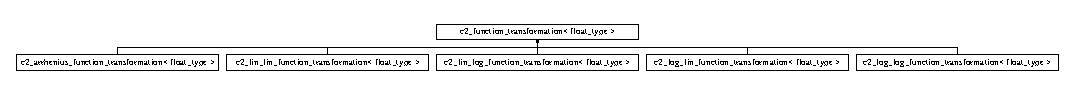
\includegraphics[height=0.715655cm]{classc2__function__transformation}
\end{center}
\end{figure}
\subsection*{Public Member Functions}
\begin{DoxyCompactItemize}
\item 
\hyperlink{classc2__function__transformation_a26fa71708edcb8b669b34daea6e9ea79}{c2\-\_\-function\-\_\-transformation} (const \hyperlink{classc2__transformation}{c2\-\_\-transformation}$<$ float\-\_\-type $>$ \&xx, const \hyperlink{classc2__transformation}{c2\-\_\-transformation}$<$ float\-\_\-type $>$ \&yy)
\begin{DoxyCompactList}\small\item\em construct this from two \hyperlink{classc2__transformation}{c2\-\_\-transformation} instances \end{DoxyCompactList}\item 
\hypertarget{classc2__function__transformation_ab7cd7a2df0c12d4ce25f2e8a415383ad}{virtual \hyperlink{classc2__function__transformation_ab7cd7a2df0c12d4ce25f2e8a415383ad}{$\sim$c2\-\_\-function\-\_\-transformation} ()}\label{classc2__function__transformation_ab7cd7a2df0c12d4ce25f2e8a415383ad}

\begin{DoxyCompactList}\small\item\em destructor \end{DoxyCompactList}\item 
virtual float\-\_\-type \hyperlink{classc2__function__transformation_a7089747852a044a4a6a9884fadecf871}{evaluate} (float\-\_\-type xraw, float\-\_\-type y, float\-\_\-type yp0, float\-\_\-type ypp0, float\-\_\-type $\ast$yprime, float\-\_\-type $\ast$yprime2) const 
\begin{DoxyCompactList}\small\item\em evaluate the transformation from internal coordinates to external coordinates \end{DoxyCompactList}\end{DoxyCompactItemize}
\subsection*{Public Attributes}
\begin{DoxyCompactItemize}
\item 
\hypertarget{classc2__function__transformation_ad6c579898f034cf8357d773ec87164a4}{const bool \hyperlink{classc2__function__transformation_ad6c579898f034cf8357d773ec87164a4}{is\-Identity}}\label{classc2__function__transformation_ad6c579898f034cf8357d773ec87164a4}

\begin{DoxyCompactList}\small\item\em flag indicating of the transform is the identity, and can be skipped for efficiency \end{DoxyCompactList}\item 
\hypertarget{classc2__function__transformation_a2bd1bd477972e8df3ed0e6d641940e92}{const \hyperlink{classc2__transformation}{c2\-\_\-transformation}\\*
$<$ float\-\_\-type $>$ \& \hyperlink{classc2__function__transformation_a2bd1bd477972e8df3ed0e6d641940e92}{X}}\label{classc2__function__transformation_a2bd1bd477972e8df3ed0e6d641940e92}

\begin{DoxyCompactList}\small\item\em the X axis transform \end{DoxyCompactList}\item 
\hypertarget{classc2__function__transformation_a867523e0adfac76943984aa5a26d4274}{const \hyperlink{classc2__transformation}{c2\-\_\-transformation}\\*
$<$ float\-\_\-type $>$ \& \hyperlink{classc2__function__transformation_a867523e0adfac76943984aa5a26d4274}{Y}}\label{classc2__function__transformation_a867523e0adfac76943984aa5a26d4274}

\begin{DoxyCompactList}\small\item\em the Y axis transform \end{DoxyCompactList}\end{DoxyCompactItemize}


\subsection{Detailed Description}
\subsubsection*{template$<$typename float\-\_\-type$>$class c2\-\_\-function\-\_\-transformation$<$ float\-\_\-type $>$}

a transformation of a function in and out of a coordinate space, using 2 c2\-\_\-transformations 

This class is a container for two axis transforms, but also provides the critical \hyperlink{classc2__function__transformation_a7089747852a044a4a6a9884fadecf871}{evaluate()} function which converts a result in internal coordinates (with derivatives) into the external representation 

\subsection{Constructor \& Destructor Documentation}
\hypertarget{classc2__function__transformation_a26fa71708edcb8b669b34daea6e9ea79}{\index{c2\-\_\-function\-\_\-transformation@{c2\-\_\-function\-\_\-transformation}!c2\-\_\-function\-\_\-transformation@{c2\-\_\-function\-\_\-transformation}}
\index{c2\-\_\-function\-\_\-transformation@{c2\-\_\-function\-\_\-transformation}!c2_function_transformation@{c2\-\_\-function\-\_\-transformation}}
\subsubsection[{c2\-\_\-function\-\_\-transformation}]{\setlength{\rightskip}{0pt plus 5cm}template$<$typename float\-\_\-type$>$ {\bf c2\-\_\-function\-\_\-transformation}$<$ float\-\_\-type $>$\-::{\bf c2\-\_\-function\-\_\-transformation} (
\begin{DoxyParamCaption}
\item[{const {\bf c2\-\_\-transformation}$<$ float\-\_\-type $>$ \&}]{xx, }
\item[{const {\bf c2\-\_\-transformation}$<$ float\-\_\-type $>$ \&}]{yy}
\end{DoxyParamCaption}
)\hspace{0.3cm}{\ttfamily [inline]}}}\label{classc2__function__transformation_a26fa71708edcb8b669b34daea6e9ea79}


construct this from two \hyperlink{classc2__transformation}{c2\-\_\-transformation} instances 


\begin{DoxyParams}{Parameters}
{\em xx} & the X axis transform \\
\hline
{\em yy} & the Y axis transform \\
\hline
\end{DoxyParams}


\subsection{Member Function Documentation}
\hypertarget{classc2__function__transformation_a7089747852a044a4a6a9884fadecf871}{\index{c2\-\_\-function\-\_\-transformation@{c2\-\_\-function\-\_\-transformation}!evaluate@{evaluate}}
\index{evaluate@{evaluate}!c2_function_transformation@{c2\-\_\-function\-\_\-transformation}}
\subsubsection[{evaluate}]{\setlength{\rightskip}{0pt plus 5cm}template$<$typename float\-\_\-type$>$ virtual float\-\_\-type {\bf c2\-\_\-function\-\_\-transformation}$<$ float\-\_\-type $>$\-::evaluate (
\begin{DoxyParamCaption}
\item[{float\-\_\-type}]{xraw, }
\item[{float\-\_\-type}]{y, }
\item[{float\-\_\-type}]{yp0, }
\item[{float\-\_\-type}]{ypp0, }
\item[{float\-\_\-type $\ast$}]{yprime, }
\item[{float\-\_\-type $\ast$}]{yprime2}
\end{DoxyParamCaption}
) const\hspace{0.3cm}{\ttfamily [virtual]}}}\label{classc2__function__transformation_a7089747852a044a4a6a9884fadecf871}


evaluate the transformation from internal coordinates to external coordinates 


\begin{DoxyParams}[1]{Parameters}
 & {\em xraw} & the value of {\itshape x} in external cordinates at which the transform is taking place \\
\hline
 & {\em y} & the value of the function in internal coordinates \\
\hline
 & {\em yp0} & the derivative in internal coordinates \\
\hline
 & {\em ypp0} & the second derivative in internal coordinates \\
\hline
\mbox{\tt out}  & {\em yprime} & pointer to the derivative, or N\-U\-L\-L, in external coordinates \\
\hline
\mbox{\tt out}  & {\em yprime2} & pointer to the second derivative, or N\-U\-L\-L, in external coordinates \\
\hline
\end{DoxyParams}
\begin{DoxyReturn}{Returns}
the value of the function in external coordinates 
\end{DoxyReturn}


The documentation for this class was generated from the following file\-:\begin{DoxyCompactItemize}
\item 
\hyperlink{c2__function_8hh}{c2\-\_\-function.\-hh}\end{DoxyCompactItemize}

\hypertarget{classc2__identity__p}{}\section{c2\+\_\+identity\+\_\+p$<$ float\+\_\+type $>$ Class Template Reference}
\label{classc2__identity__p}\index{c2\+\_\+identity\+\_\+p$<$ float\+\_\+type $>$@{c2\+\_\+identity\+\_\+p$<$ float\+\_\+type $>$}}


compute x with its derivatives.

The factory function \hyperlink{classc2__factory_a66970667d203c0e63a016b08d2472dc4}{c2\+\_\+factory\+::identity()} creates $\ast$new \hyperlink{classc2__identity__p}{c2\+\_\+identity\+\_\+p}  




{\ttfamily \#include \char`\"{}c2\+\_\+function.\+hh\char`\"{}}



Inheritance diagram for c2\+\_\+identity\+\_\+p$<$ float\+\_\+type $>$\+:
\nopagebreak
\begin{figure}[H]
\begin{center}
\leavevmode
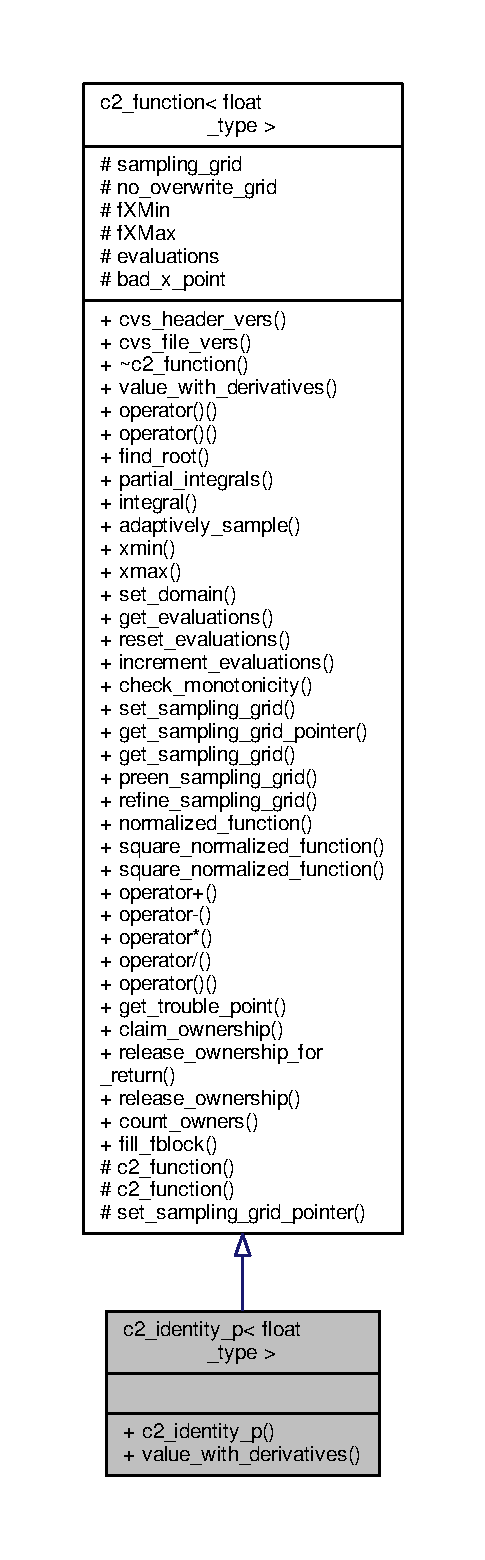
\includegraphics[height=550pt]{classc2__identity__p__inherit__graph}
\end{center}
\end{figure}


Collaboration diagram for c2\+\_\+identity\+\_\+p$<$ float\+\_\+type $>$\+:
\nopagebreak
\begin{figure}[H]
\begin{center}
\leavevmode
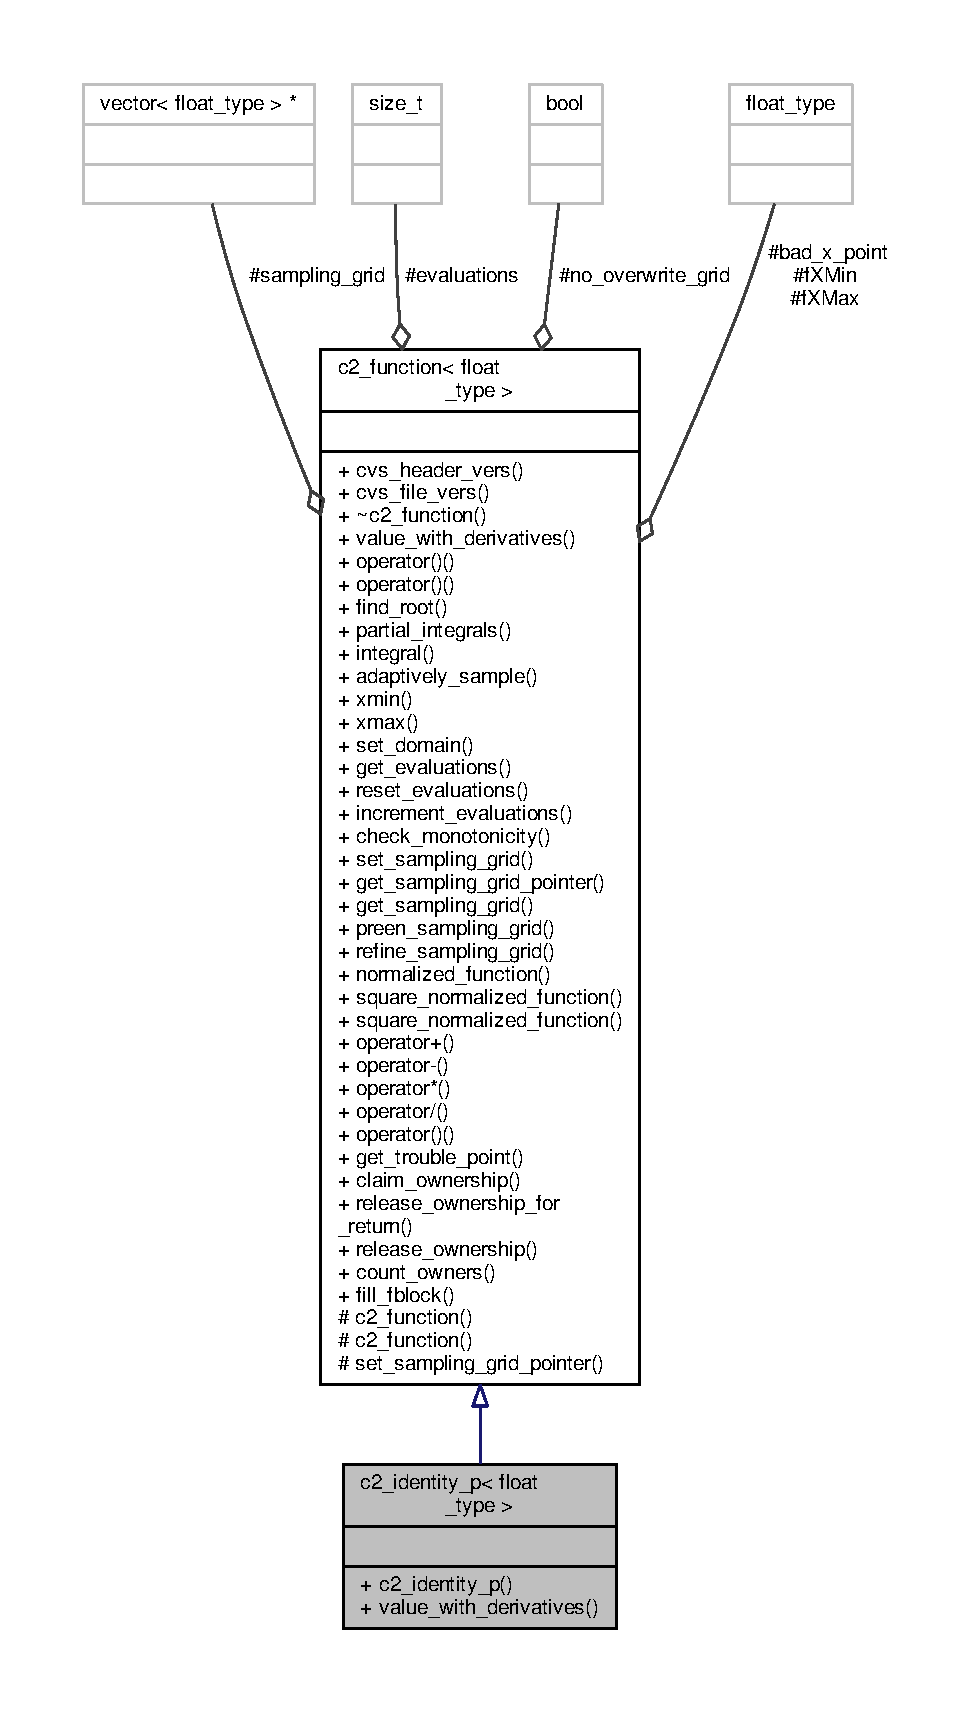
\includegraphics[height=550pt]{classc2__identity__p__coll__graph}
\end{center}
\end{figure}
\subsection*{Public Member Functions}
\begin{DoxyCompactItemize}
\item 
\hyperlink{classc2__identity__p_a9b00bbd9a2dc1572cf75e38019cfed94}{c2\+\_\+identity\+\_\+p} ()
\begin{DoxyCompactList}\small\item\em constructor. \end{DoxyCompactList}\item 
virtual float\+\_\+type \hyperlink{classc2__identity__p_a69a30999382af761b9360179dbedbc88}{value\+\_\+with\+\_\+derivatives} (float\+\_\+type x, float\+\_\+type $\ast$yprime, float\+\_\+type $\ast$yprime2) const   throw (c2\+\_\+exception)
\begin{DoxyCompactList}\small\item\em get the value and derivatives. \end{DoxyCompactList}\end{DoxyCompactItemize}
\subsection*{Additional Inherited Members}


\subsection{Detailed Description}
\subsubsection*{template$<$typename float\+\_\+type = double$>$\\*
class c2\+\_\+identity\+\_\+p$<$ float\+\_\+type $>$}

compute x with its derivatives.

The factory function \hyperlink{classc2__factory_a66970667d203c0e63a016b08d2472dc4}{c2\+\_\+factory\+::identity()} creates $\ast$new \hyperlink{classc2__identity__p}{c2\+\_\+identity\+\_\+p} 

\subsection{Constructor \& Destructor Documentation}
\index{c2\+\_\+identity\+\_\+p@{c2\+\_\+identity\+\_\+p}!c2\+\_\+identity\+\_\+p@{c2\+\_\+identity\+\_\+p}}
\index{c2\+\_\+identity\+\_\+p@{c2\+\_\+identity\+\_\+p}!c2\+\_\+identity\+\_\+p@{c2\+\_\+identity\+\_\+p}}
\subsubsection[{\texorpdfstring{c2\+\_\+identity\+\_\+p()}{c2_identity_p()}}]{\setlength{\rightskip}{0pt plus 5cm}template$<$typename float\+\_\+type  = double$>$ {\bf c2\+\_\+identity\+\_\+p}$<$ float\+\_\+type $>$\+::{\bf c2\+\_\+identity\+\_\+p} (
\begin{DoxyParamCaption}
{}
\end{DoxyParamCaption}
)\hspace{0.3cm}{\ttfamily [inline]}}\hypertarget{classc2__identity__p_a9b00bbd9a2dc1572cf75e38019cfed94}{}\label{classc2__identity__p_a9b00bbd9a2dc1572cf75e38019cfed94}


constructor. 



\subsection{Member Function Documentation}
\index{c2\+\_\+identity\+\_\+p@{c2\+\_\+identity\+\_\+p}!value\+\_\+with\+\_\+derivatives@{value\+\_\+with\+\_\+derivatives}}
\index{value\+\_\+with\+\_\+derivatives@{value\+\_\+with\+\_\+derivatives}!c2\+\_\+identity\+\_\+p@{c2\+\_\+identity\+\_\+p}}
\subsubsection[{\texorpdfstring{value\+\_\+with\+\_\+derivatives(float\+\_\+type x, float\+\_\+type $\ast$yprime, float\+\_\+type $\ast$yprime2) const }{value_with_derivatives(float_type x, float_type *yprime, float_type *yprime2) const }}]{\setlength{\rightskip}{0pt plus 5cm}template$<$typename float\+\_\+type  = double$>$ virtual float\+\_\+type {\bf c2\+\_\+identity\+\_\+p}$<$ float\+\_\+type $>$\+::value\+\_\+with\+\_\+derivatives (
\begin{DoxyParamCaption}
\item[{float\+\_\+type}]{x, }
\item[{float\+\_\+type $\ast$}]{yprime, }
\item[{float\+\_\+type $\ast$}]{yprime2}
\end{DoxyParamCaption}
) const throw  {\bf c2\+\_\+exception}) \hspace{0.3cm}{\ttfamily [inline]}, {\ttfamily [virtual]}}\hypertarget{classc2__identity__p_a69a30999382af761b9360179dbedbc88}{}\label{classc2__identity__p_a69a30999382af761b9360179dbedbc88}


get the value and derivatives. 

There is required checking for null pointers on the derivatives, and most implementations should operate faster if derivatives are not needed. 
\begin{DoxyParams}[1]{Parameters}
\mbox{\tt in}  & {\em x} & the point at which to evaluate the function \\
\hline
\mbox{\tt out}  & {\em yprime} & the first derivative (if pointer is non-\/null) \\
\hline
\mbox{\tt out}  & {\em yprime2} & the second derivative (if pointer is non-\/null) \\
\hline
\end{DoxyParams}
\begin{DoxyReturn}{Returns}
the value of the function 
\end{DoxyReturn}


Implements \hyperlink{classc2__function_a44e0201159111350be7f746fc9026f67}{c2\+\_\+function$<$ float\+\_\+type $>$}.



The documentation for this class was generated from the following file\+:\begin{DoxyCompactItemize}
\item 
\hyperlink{c2__function_8hh}{c2\+\_\+function.\+hh}\end{DoxyCompactItemize}

\hypertarget{classc2__inverse__function__p}{\section{c2\-\_\-inverse\-\_\-function\-\_\-p$<$ float\-\_\-type $>$ Class Template Reference}
\label{classc2__inverse__function__p}\index{c2\-\_\-inverse\-\_\-function\-\_\-p$<$ float\-\_\-type $>$@{c2\-\_\-inverse\-\_\-function\-\_\-p$<$ float\-\_\-type $>$}}
}


create the formal inverse function of another function

for example, given a \hyperlink{classc2__function}{c2\-\_\-function} {\itshape f}  




{\ttfamily \#include $<$c2\-\_\-function.\-hh$>$}

Inheritance diagram for c2\-\_\-inverse\-\_\-function\-\_\-p$<$ float\-\_\-type $>$\-:\begin{figure}[H]
\begin{center}
\leavevmode
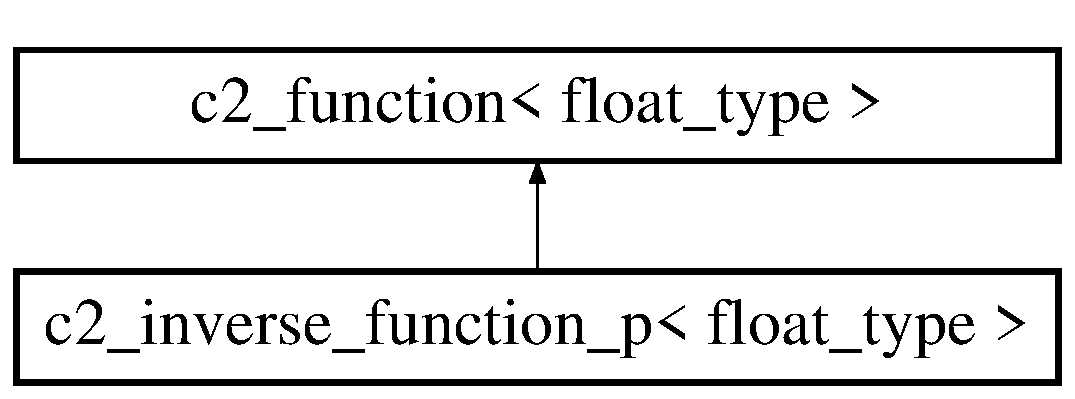
\includegraphics[height=2.000000cm]{classc2__inverse__function__p}
\end{center}
\end{figure}
\subsection*{Public Member Functions}
\begin{DoxyCompactItemize}
\item 
\hyperlink{classc2__inverse__function__p_a764ddeb41fcf06a36c3435be12bf7611}{c2\-\_\-inverse\-\_\-function\-\_\-p} (const \hyperlink{classc2__function}{c2\-\_\-function}$<$ float\-\_\-type $>$ \&source)
\begin{DoxyCompactList}\small\item\em Construct the operator. \end{DoxyCompactList}\item 
virtual float\-\_\-type \hyperlink{classc2__inverse__function__p_a907dbfc4a1ea0530ae76a1ae8704f8ce}{value\-\_\-with\-\_\-derivatives} (float\-\_\-type x, float\-\_\-type $\ast$yprime, float\-\_\-type $\ast$yprime2) const   throw (c2\-\_\-exception)
\begin{DoxyCompactList}\small\item\em get the value and derivatives. \end{DoxyCompactList}\item 
void \hyperlink{classc2__inverse__function__p_a71c6d3be4ae949024979f0968c5bf1f4}{set\-\_\-start\-\_\-hint} (float\-\_\-type hint) const 
\begin{DoxyCompactList}\small\item\em give the function a hint as to where to look for its inverse \end{DoxyCompactList}\item 
virtual float\-\_\-type \hyperlink{classc2__inverse__function__p_a49eac4019f5e0213c9d2111a1007b699}{get\-\_\-start\-\_\-hint} (float\-\_\-type x) const 
\begin{DoxyCompactList}\small\item\em get the starting hint. \end{DoxyCompactList}\item 
void \hyperlink{classc2__inverse__function__p_a69e1d30e9266238303183b25cdcf19ce}{set\-\_\-hinting\-\_\-function} (const \hyperlink{classc2__function}{c2\-\_\-function}$<$ float\-\_\-type $>$ $\ast$hint\-\_\-func)
\begin{DoxyCompactList}\small\item\em set or unset the approximate function used to start the root finder \end{DoxyCompactList}\item 
void \hyperlink{classc2__inverse__function__p_aa8e91ae51b9d0a0f7085f6bd512574fa}{set\-\_\-hinting\-\_\-function} (const \hyperlink{classc2__const__ptr}{c2\-\_\-const\-\_\-ptr}$<$ float\-\_\-type $>$ hint\-\_\-func)
\begin{DoxyCompactList}\small\item\em set the hinting function from a pointer. \end{DoxyCompactList}\end{DoxyCompactItemize}
\subsection*{Protected Attributes}
\begin{DoxyCompactItemize}
\item 
\hypertarget{classc2__inverse__function__p_a1d5e1f16d32ff5e8fef9e239ff5c18ed}{float\-\_\-type {\bfseries start\-\_\-hint}}\label{classc2__inverse__function__p_a1d5e1f16d32ff5e8fef9e239ff5c18ed}

\item 
\hypertarget{classc2__inverse__function__p_af8d083863a7965e901c684de7bd3cf8f}{const \hyperlink{classc2__const__ptr}{c2\-\_\-const\-\_\-ptr}$<$ float\-\_\-type $>$ {\bfseries func}}\label{classc2__inverse__function__p_af8d083863a7965e901c684de7bd3cf8f}

\item 
\hypertarget{classc2__inverse__function__p_a4e1f68a44dea194ec1737fdcc8a7f17f}{\hyperlink{classc2__const__ptr}{c2\-\_\-const\-\_\-ptr}$<$ float\-\_\-type $>$ {\bfseries hinting\-\_\-function}}\label{classc2__inverse__function__p_a4e1f68a44dea194ec1737fdcc8a7f17f}

\end{DoxyCompactItemize}
\subsection*{Additional Inherited Members}


\subsection{Detailed Description}
\subsubsection*{template$<$typename float\-\_\-type = double$>$class c2\-\_\-inverse\-\_\-function\-\_\-p$<$ float\-\_\-type $>$}

create the formal inverse function of another function

for example, given a \hyperlink{classc2__function}{c2\-\_\-function} {\itshape f} 


\begin{DoxyCode}
c2\_inverse\_function<double> inv(f);
a=f(x);
x1=inv(a);
\end{DoxyCode}
 will return x1=x to machine precision. The important part of this is that the resulting function is a first-\/class \hyperlink{classc2__function}{c2\-\_\-function}, so it knows its derivatives, too, unlike the case of a simple root-\/finding inverse. This means it can be integrated (for example) quite efficiently.

\begin{DoxySeeAlso}{See Also}
combined\-\_\-inversion\-\_\-hinting\-\_\-sampling
\end{DoxySeeAlso}
The factory function \hyperlink{classc2__factory_aecac3e5856e36ea582da455f1b94c4d7}{c2\-\_\-factory\-::inverse\-\_\-function()} creates $\ast$new \hyperlink{classc2__inverse__function__p}{c2\-\_\-inverse\-\_\-function\-\_\-p} 

\subsection{Constructor \& Destructor Documentation}
\hypertarget{classc2__inverse__function__p_a764ddeb41fcf06a36c3435be12bf7611}{\index{c2\-\_\-inverse\-\_\-function\-\_\-p@{c2\-\_\-inverse\-\_\-function\-\_\-p}!c2\-\_\-inverse\-\_\-function\-\_\-p@{c2\-\_\-inverse\-\_\-function\-\_\-p}}
\index{c2\-\_\-inverse\-\_\-function\-\_\-p@{c2\-\_\-inverse\-\_\-function\-\_\-p}!c2_inverse_function_p@{c2\-\_\-inverse\-\_\-function\-\_\-p}}
\subsubsection[{c2\-\_\-inverse\-\_\-function\-\_\-p}]{\setlength{\rightskip}{0pt plus 5cm}template$<$typename float\-\_\-type  = double$>$ {\bf c2\-\_\-inverse\-\_\-function\-\_\-p}$<$ float\-\_\-type $>$\-::{\bf c2\-\_\-inverse\-\_\-function\-\_\-p} (
\begin{DoxyParamCaption}
\item[{const {\bf c2\-\_\-function}$<$ float\-\_\-type $>$ \&}]{source}
\end{DoxyParamCaption}
)}}\label{classc2__inverse__function__p_a764ddeb41fcf06a36c3435be12bf7611}


Construct the operator. 


\begin{DoxyParams}{Parameters}
{\em source} & the function to be inverted \\
\hline
\end{DoxyParams}


\subsection{Member Function Documentation}
\hypertarget{classc2__inverse__function__p_a49eac4019f5e0213c9d2111a1007b699}{\index{c2\-\_\-inverse\-\_\-function\-\_\-p@{c2\-\_\-inverse\-\_\-function\-\_\-p}!get\-\_\-start\-\_\-hint@{get\-\_\-start\-\_\-hint}}
\index{get\-\_\-start\-\_\-hint@{get\-\_\-start\-\_\-hint}!c2_inverse_function_p@{c2\-\_\-inverse\-\_\-function\-\_\-p}}
\subsubsection[{get\-\_\-start\-\_\-hint}]{\setlength{\rightskip}{0pt plus 5cm}template$<$typename float\-\_\-type  = double$>$ virtual float\-\_\-type {\bf c2\-\_\-inverse\-\_\-function\-\_\-p}$<$ float\-\_\-type $>$\-::get\-\_\-start\-\_\-hint (
\begin{DoxyParamCaption}
\item[{float\-\_\-type}]{x}
\end{DoxyParamCaption}
) const\hspace{0.3cm}{\ttfamily [inline]}, {\ttfamily [virtual]}}}\label{classc2__inverse__function__p_a49eac4019f5e0213c9d2111a1007b699}


get the starting hint. 

This is virtual so if there is a better way, this can be easily overridden. It is used in \hyperlink{classc2__inverse__function__p_a907dbfc4a1ea0530ae76a1ae8704f8ce}{value\-\_\-with\-\_\-derivatives()} to guess where to start the root finder. 
\begin{DoxyParams}{Parameters}
{\em x} & the abscissa for which an estimate is needed \\
\hline
\end{DoxyParams}
\hypertarget{classc2__inverse__function__p_a69e1d30e9266238303183b25cdcf19ce}{\index{c2\-\_\-inverse\-\_\-function\-\_\-p@{c2\-\_\-inverse\-\_\-function\-\_\-p}!set\-\_\-hinting\-\_\-function@{set\-\_\-hinting\-\_\-function}}
\index{set\-\_\-hinting\-\_\-function@{set\-\_\-hinting\-\_\-function}!c2_inverse_function_p@{c2\-\_\-inverse\-\_\-function\-\_\-p}}
\subsubsection[{set\-\_\-hinting\-\_\-function}]{\setlength{\rightskip}{0pt plus 5cm}template$<$typename float\-\_\-type  = double$>$ void {\bf c2\-\_\-inverse\-\_\-function\-\_\-p}$<$ float\-\_\-type $>$\-::set\-\_\-hinting\-\_\-function (
\begin{DoxyParamCaption}
\item[{const {\bf c2\-\_\-function}$<$ float\-\_\-type $>$ $\ast$}]{hint\-\_\-func}
\end{DoxyParamCaption}
)\hspace{0.3cm}{\ttfamily [inline]}}}\label{classc2__inverse__function__p_a69e1d30e9266238303183b25cdcf19ce}


set or unset the approximate function used to start the root finder 

\label{classc2__inverse__function__p_set_hinting_function_discussion}%
\hypertarget{classc2__inverse__function__p_set_hinting_function_discussion}{}%
A hinting function is mostly useful if the evaluation of this inverse is going to be carried out in very non-\/local order, so the root finder has to start over for each step. If most evaluations are going to be made in fairly localized clusters (scanning through the function, for example), the default mechanism used (which just remembers the last point) is almost certainly faster.

Typically, the hinting function is likely to be set up by creating the inverse function, and then adaptively sampling an interpolating function from it, and then using the result to hint it. Another way, if the parent function is already an interpolating function, is just to create a version of the parent with the x \& y coordinates reversed.

\begin{DoxySeeAlso}{See Also}
combined\-\_\-inversion\-\_\-hinting\-\_\-sampling
\end{DoxySeeAlso}

\begin{DoxyParams}{Parameters}
{\em hint\-\_\-func} & the function that is an approximate inverse of the parent of this inverse\-\_\-function \\
\hline
\end{DoxyParams}
\hypertarget{classc2__inverse__function__p_aa8e91ae51b9d0a0f7085f6bd512574fa}{\index{c2\-\_\-inverse\-\_\-function\-\_\-p@{c2\-\_\-inverse\-\_\-function\-\_\-p}!set\-\_\-hinting\-\_\-function@{set\-\_\-hinting\-\_\-function}}
\index{set\-\_\-hinting\-\_\-function@{set\-\_\-hinting\-\_\-function}!c2_inverse_function_p@{c2\-\_\-inverse\-\_\-function\-\_\-p}}
\subsubsection[{set\-\_\-hinting\-\_\-function}]{\setlength{\rightskip}{0pt plus 5cm}template$<$typename float\-\_\-type  = double$>$ void {\bf c2\-\_\-inverse\-\_\-function\-\_\-p}$<$ float\-\_\-type $>$\-::set\-\_\-hinting\-\_\-function (
\begin{DoxyParamCaption}
\item[{const {\bf c2\-\_\-const\-\_\-ptr}$<$ float\-\_\-type $>$}]{hint\-\_\-func}
\end{DoxyParamCaption}
)\hspace{0.3cm}{\ttfamily [inline]}}}\label{classc2__inverse__function__p_aa8e91ae51b9d0a0f7085f6bd512574fa}


set the hinting function from a pointer. 

See \hyperlink{classc2__inverse__function__p_set_hinting_function_discussion}{discussion} 
\begin{DoxyParams}{Parameters}
{\em hint\-\_\-func} & the container holding the function \\
\hline
\end{DoxyParams}
\hypertarget{classc2__inverse__function__p_a71c6d3be4ae949024979f0968c5bf1f4}{\index{c2\-\_\-inverse\-\_\-function\-\_\-p@{c2\-\_\-inverse\-\_\-function\-\_\-p}!set\-\_\-start\-\_\-hint@{set\-\_\-start\-\_\-hint}}
\index{set\-\_\-start\-\_\-hint@{set\-\_\-start\-\_\-hint}!c2_inverse_function_p@{c2\-\_\-inverse\-\_\-function\-\_\-p}}
\subsubsection[{set\-\_\-start\-\_\-hint}]{\setlength{\rightskip}{0pt plus 5cm}template$<$typename float\-\_\-type  = double$>$ void {\bf c2\-\_\-inverse\-\_\-function\-\_\-p}$<$ float\-\_\-type $>$\-::set\-\_\-start\-\_\-hint (
\begin{DoxyParamCaption}
\item[{float\-\_\-type}]{hint}
\end{DoxyParamCaption}
) const\hspace{0.3cm}{\ttfamily [inline]}}}\label{classc2__inverse__function__p_a71c6d3be4ae949024979f0968c5bf1f4}


give the function a hint as to where to look for its inverse 


\begin{DoxyParams}{Parameters}
{\em hint} & the likely value of the inverse, which defaults to whatever the evaluation returned. \\
\hline
\end{DoxyParams}
\hypertarget{classc2__inverse__function__p_a907dbfc4a1ea0530ae76a1ae8704f8ce}{\index{c2\-\_\-inverse\-\_\-function\-\_\-p@{c2\-\_\-inverse\-\_\-function\-\_\-p}!value\-\_\-with\-\_\-derivatives@{value\-\_\-with\-\_\-derivatives}}
\index{value\-\_\-with\-\_\-derivatives@{value\-\_\-with\-\_\-derivatives}!c2_inverse_function_p@{c2\-\_\-inverse\-\_\-function\-\_\-p}}
\subsubsection[{value\-\_\-with\-\_\-derivatives}]{\setlength{\rightskip}{0pt plus 5cm}template$<$typename float\-\_\-type  = double$>$ virtual float\-\_\-type {\bf c2\-\_\-inverse\-\_\-function\-\_\-p}$<$ float\-\_\-type $>$\-::value\-\_\-with\-\_\-derivatives (
\begin{DoxyParamCaption}
\item[{float\-\_\-type}]{x, }
\item[{float\-\_\-type $\ast$}]{yprime, }
\item[{float\-\_\-type $\ast$}]{yprime2}
\end{DoxyParamCaption}
) const throw  {\bf c2\-\_\-exception}) \hspace{0.3cm}{\ttfamily [virtual]}}}\label{classc2__inverse__function__p_a907dbfc4a1ea0530ae76a1ae8704f8ce}


get the value and derivatives. 

There is required checking for null pointers on the derivatives, and most implementations should operate faster if derivatives are not needed. 
\begin{DoxyParams}[1]{Parameters}
\mbox{\tt in}  & {\em x} & the point at which to evaluate the function \\
\hline
\mbox{\tt out}  & {\em yprime} & the first derivative (if pointer is non-\/null) \\
\hline
\mbox{\tt out}  & {\em yprime2} & the second derivative (if pointer is non-\/null) \\
\hline
\end{DoxyParams}
\begin{DoxyReturn}{Returns}
the value of the function 
\end{DoxyReturn}


Implements \hyperlink{classc2__function_a44e0201159111350be7f746fc9026f67}{c2\-\_\-function$<$ float\-\_\-type $>$}.



The documentation for this class was generated from the following file\-:\begin{DoxyCompactItemize}
\item 
\hyperlink{c2__function_8hh}{c2\-\_\-function.\-hh}\end{DoxyCompactItemize}

\hypertarget{classc2__lin__lin__function__transformation}{\section{c2\-\_\-lin\-\_\-lin\-\_\-function\-\_\-transformation$<$ float\-\_\-type $>$ Class Template Reference}
\label{classc2__lin__lin__function__transformation}\index{c2\-\_\-lin\-\_\-lin\-\_\-function\-\_\-transformation$<$ float\-\_\-type $>$@{c2\-\_\-lin\-\_\-lin\-\_\-function\-\_\-transformation$<$ float\-\_\-type $>$}}
}


a transformation of a function in and out of lin-\/lin space  




{\ttfamily \#include $<$c2\-\_\-function.\-hh$>$}

Inheritance diagram for c2\-\_\-lin\-\_\-lin\-\_\-function\-\_\-transformation$<$ float\-\_\-type $>$\-:\begin{figure}[H]
\begin{center}
\leavevmode
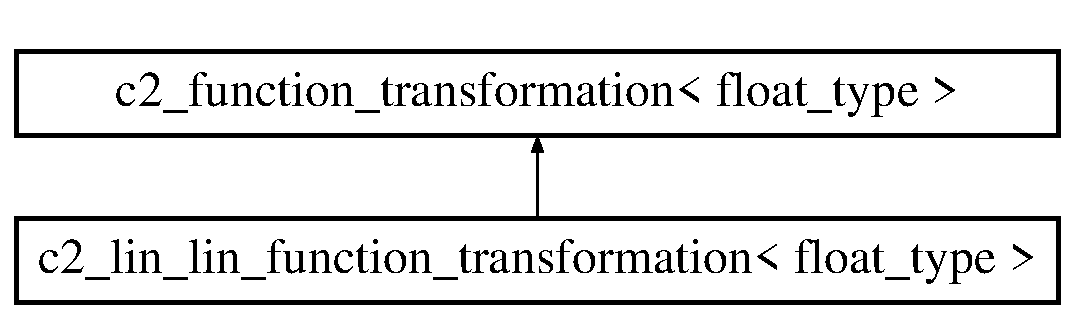
\includegraphics[height=2.000000cm]{classc2__lin__lin__function__transformation}
\end{center}
\end{figure}
\subsection*{Additional Inherited Members}


\subsection{Detailed Description}
\subsubsection*{template$<$typename float\-\_\-type$>$class c2\-\_\-lin\-\_\-lin\-\_\-function\-\_\-transformation$<$ float\-\_\-type $>$}

a transformation of a function in and out of lin-\/lin space 



The documentation for this class was generated from the following file\-:\begin{DoxyCompactItemize}
\item 
\hyperlink{c2__function_8hh}{c2\-\_\-function.\-hh}\end{DoxyCompactItemize}

\hypertarget{classc2__lin__log__function__transformation}{}\section{c2\+\_\+lin\+\_\+log\+\_\+function\+\_\+transformation$<$ float\+\_\+type $>$ Class Template Reference}
\label{classc2__lin__log__function__transformation}\index{c2\+\_\+lin\+\_\+log\+\_\+function\+\_\+transformation$<$ float\+\_\+type $>$@{c2\+\_\+lin\+\_\+log\+\_\+function\+\_\+transformation$<$ float\+\_\+type $>$}}


a transformation of a function in and out of lin-\/log space  




{\ttfamily \#include \char`\"{}c2\+\_\+function.\+hh\char`\"{}}



Inheritance diagram for c2\+\_\+lin\+\_\+log\+\_\+function\+\_\+transformation$<$ float\+\_\+type $>$\+:
\nopagebreak
\begin{figure}[H]
\begin{center}
\leavevmode
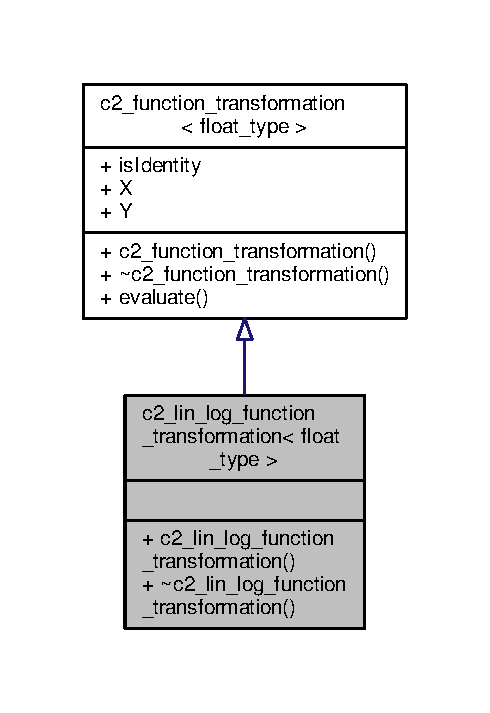
\includegraphics[width=235pt]{classc2__lin__log__function__transformation__inherit__graph}
\end{center}
\end{figure}


Collaboration diagram for c2\+\_\+lin\+\_\+log\+\_\+function\+\_\+transformation$<$ float\+\_\+type $>$\+:
\nopagebreak
\begin{figure}[H]
\begin{center}
\leavevmode
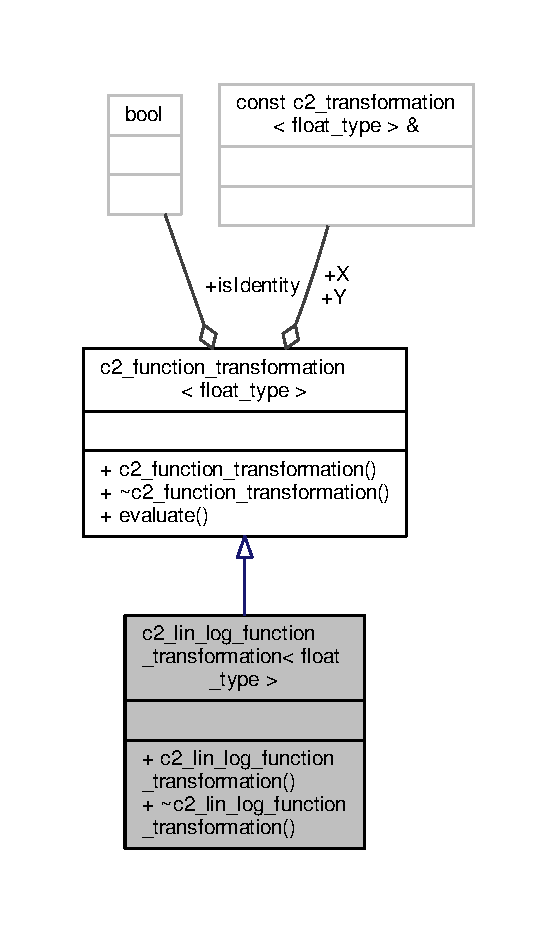
\includegraphics[width=268pt]{classc2__lin__log__function__transformation__coll__graph}
\end{center}
\end{figure}
\subsection*{Public Member Functions}
\begin{DoxyCompactItemize}
\item 
\hyperlink{classc2__lin__log__function__transformation_ac37bc1e464ecf93b21a9b47a8839d1ea}{c2\+\_\+lin\+\_\+log\+\_\+function\+\_\+transformation} ()
\item 
virtual \hyperlink{classc2__lin__log__function__transformation_a12ef189ce688be24d4ce7699e20d3c0b}{$\sim$c2\+\_\+lin\+\_\+log\+\_\+function\+\_\+transformation} ()
\end{DoxyCompactItemize}
\subsection*{Additional Inherited Members}


\subsection{Detailed Description}
\subsubsection*{template$<$typename float\+\_\+type$>$\\*
class c2\+\_\+lin\+\_\+log\+\_\+function\+\_\+transformation$<$ float\+\_\+type $>$}

a transformation of a function in and out of lin-\/log space 



\subsection{Constructor \& Destructor Documentation}
\index{c2\+\_\+lin\+\_\+log\+\_\+function\+\_\+transformation@{c2\+\_\+lin\+\_\+log\+\_\+function\+\_\+transformation}!c2\+\_\+lin\+\_\+log\+\_\+function\+\_\+transformation@{c2\+\_\+lin\+\_\+log\+\_\+function\+\_\+transformation}}
\index{c2\+\_\+lin\+\_\+log\+\_\+function\+\_\+transformation@{c2\+\_\+lin\+\_\+log\+\_\+function\+\_\+transformation}!c2\+\_\+lin\+\_\+log\+\_\+function\+\_\+transformation@{c2\+\_\+lin\+\_\+log\+\_\+function\+\_\+transformation}}
\subsubsection[{\texorpdfstring{c2\+\_\+lin\+\_\+log\+\_\+function\+\_\+transformation()}{c2_lin_log_function_transformation()}}]{\setlength{\rightskip}{0pt plus 5cm}template$<$typename float\+\_\+type $>$ {\bf c2\+\_\+lin\+\_\+log\+\_\+function\+\_\+transformation}$<$ float\+\_\+type $>$\+::{\bf c2\+\_\+lin\+\_\+log\+\_\+function\+\_\+transformation} (
\begin{DoxyParamCaption}
{}
\end{DoxyParamCaption}
)\hspace{0.3cm}{\ttfamily [inline]}}\hypertarget{classc2__lin__log__function__transformation_ac37bc1e464ecf93b21a9b47a8839d1ea}{}\label{classc2__lin__log__function__transformation_ac37bc1e464ecf93b21a9b47a8839d1ea}
\index{c2\+\_\+lin\+\_\+log\+\_\+function\+\_\+transformation@{c2\+\_\+lin\+\_\+log\+\_\+function\+\_\+transformation}!````~c2\+\_\+lin\+\_\+log\+\_\+function\+\_\+transformation@{$\sim$c2\+\_\+lin\+\_\+log\+\_\+function\+\_\+transformation}}
\index{````~c2\+\_\+lin\+\_\+log\+\_\+function\+\_\+transformation@{$\sim$c2\+\_\+lin\+\_\+log\+\_\+function\+\_\+transformation}!c2\+\_\+lin\+\_\+log\+\_\+function\+\_\+transformation@{c2\+\_\+lin\+\_\+log\+\_\+function\+\_\+transformation}}
\subsubsection[{\texorpdfstring{$\sim$c2\+\_\+lin\+\_\+log\+\_\+function\+\_\+transformation()}{~c2_lin_log_function_transformation()}}]{\setlength{\rightskip}{0pt plus 5cm}template$<$typename float\+\_\+type $>$ virtual {\bf c2\+\_\+lin\+\_\+log\+\_\+function\+\_\+transformation}$<$ float\+\_\+type $>$\+::$\sim${\bf c2\+\_\+lin\+\_\+log\+\_\+function\+\_\+transformation} (
\begin{DoxyParamCaption}
{}
\end{DoxyParamCaption}
)\hspace{0.3cm}{\ttfamily [inline]}, {\ttfamily [virtual]}}\hypertarget{classc2__lin__log__function__transformation_a12ef189ce688be24d4ce7699e20d3c0b}{}\label{classc2__lin__log__function__transformation_a12ef189ce688be24d4ce7699e20d3c0b}


The documentation for this class was generated from the following file\+:\begin{DoxyCompactItemize}
\item 
\hyperlink{c2__function_8hh}{c2\+\_\+function.\+hh}\end{DoxyCompactItemize}

\hypertarget{classc2__linear__p}{\section{c2\-\_\-linear\-\_\-p$<$ float\-\_\-type $>$ Class Template Reference}
\label{classc2__linear__p}\index{c2\-\_\-linear\-\_\-p$<$ float\-\_\-type $>$@{c2\-\_\-linear\-\_\-p$<$ float\-\_\-type $>$}}
}


create a linear mapping of another function

for example, given a \hyperlink{classc2__function}{c2\-\_\-function} {\itshape f}  




{\ttfamily \#include $<$c2\-\_\-function.\-hh$>$}

Inheritance diagram for c2\-\_\-linear\-\_\-p$<$ float\-\_\-type $>$\-:\begin{figure}[H]
\begin{center}
\leavevmode
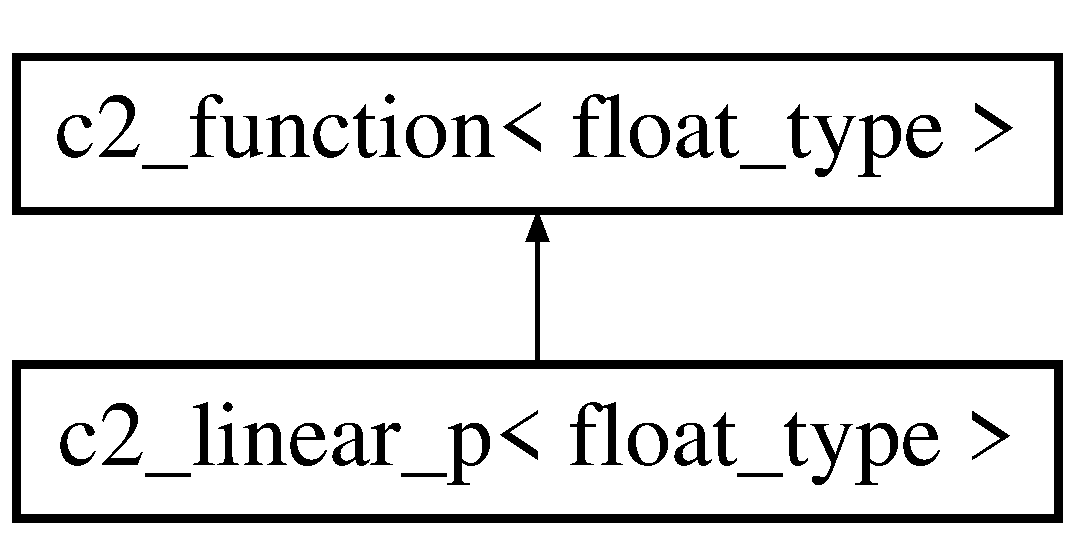
\includegraphics[height=2.000000cm]{classc2__linear__p}
\end{center}
\end{figure}
\subsection*{Public Member Functions}
\begin{DoxyCompactItemize}
\item 
\hyperlink{classc2__linear__p_a6a76eba066b8f52636fd4b6cc7307b06}{c2\-\_\-linear\-\_\-p} (float\-\_\-type x0, float\-\_\-type y0, float\-\_\-type slope)
\begin{DoxyCompactList}\small\item\em Construct the operator f=y0 + slope $\ast$ (x-\/x0) \end{DoxyCompactList}\item 
void \hyperlink{classc2__linear__p_ada2849448ebb2b5b493f45a2db6ab908}{reset} (float\-\_\-type x0, float\-\_\-type y0, float\-\_\-type slope)
\begin{DoxyCompactList}\small\item\em Change the slope and intercepts after construction. \end{DoxyCompactList}\item 
virtual float\-\_\-type \hyperlink{classc2__linear__p_a1d6ce127c8e991c4293f530f341ce617}{value\-\_\-with\-\_\-derivatives} (float\-\_\-type x, float\-\_\-type $\ast$yprime, float\-\_\-type $\ast$yprime2) const   throw (c2\-\_\-exception)
\begin{DoxyCompactList}\small\item\em get the value and derivatives. \end{DoxyCompactList}\end{DoxyCompactItemize}
\subsection*{Additional Inherited Members}


\subsection{Detailed Description}
\subsubsection*{template$<$typename float\-\_\-type = double$>$class c2\-\_\-linear\-\_\-p$<$ float\-\_\-type $>$}

create a linear mapping of another function

for example, given a \hyperlink{classc2__function}{c2\-\_\-function} {\itshape f} 


\begin{DoxyCode}
\hyperlink{classc2__function}{c2\_function<double>} &F=c2\_linear<double>(1.2, 2.0, 3.0)(f);
\end{DoxyCode}
 produces a new \hyperlink{classc2__function}{c2\-\_\-function} F=2.\-0+3.0$\ast$({\itshape f} -\/ 1.\-2)

The factory function \hyperlink{classc2__factory_a2113dc577f24931e0cf316137faf557c}{c2\-\_\-factory\-::linear()} creates $\ast$new \hyperlink{classc2__linear__p}{c2\-\_\-linear\-\_\-p} 

\subsection{Constructor \& Destructor Documentation}
\hypertarget{classc2__linear__p_a6a76eba066b8f52636fd4b6cc7307b06}{\index{c2\-\_\-linear\-\_\-p@{c2\-\_\-linear\-\_\-p}!c2\-\_\-linear\-\_\-p@{c2\-\_\-linear\-\_\-p}}
\index{c2\-\_\-linear\-\_\-p@{c2\-\_\-linear\-\_\-p}!c2_linear_p@{c2\-\_\-linear\-\_\-p}}
\subsubsection[{c2\-\_\-linear\-\_\-p}]{\setlength{\rightskip}{0pt plus 5cm}template$<$typename float\-\_\-type = double$>$ {\bf c2\-\_\-linear\-\_\-p}$<$ float\-\_\-type $>$\-::{\bf c2\-\_\-linear\-\_\-p} (
\begin{DoxyParamCaption}
\item[{float\-\_\-type}]{x0, }
\item[{float\-\_\-type}]{y0, }
\item[{float\-\_\-type}]{slope}
\end{DoxyParamCaption}
)\hspace{0.3cm}{\ttfamily [inline]}}}\label{classc2__linear__p_a6a76eba066b8f52636fd4b6cc7307b06}


Construct the operator f=y0 + slope $\ast$ (x-\/x0) 


\begin{DoxyParams}{Parameters}
{\em x0} & the x offset \\
\hline
{\em y0} & the y-\/intercept i.\-e. f(x0) \\
\hline
{\em slope} & the slope of the mapping \\
\hline
\end{DoxyParams}


\subsection{Member Function Documentation}
\hypertarget{classc2__linear__p_ada2849448ebb2b5b493f45a2db6ab908}{\index{c2\-\_\-linear\-\_\-p@{c2\-\_\-linear\-\_\-p}!reset@{reset}}
\index{reset@{reset}!c2_linear_p@{c2\-\_\-linear\-\_\-p}}
\subsubsection[{reset}]{\setlength{\rightskip}{0pt plus 5cm}template$<$typename float\-\_\-type = double$>$ void {\bf c2\-\_\-linear\-\_\-p}$<$ float\-\_\-type $>$\-::reset (
\begin{DoxyParamCaption}
\item[{float\-\_\-type}]{x0, }
\item[{float\-\_\-type}]{y0, }
\item[{float\-\_\-type}]{slope}
\end{DoxyParamCaption}
)\hspace{0.3cm}{\ttfamily [inline]}}}\label{classc2__linear__p_ada2849448ebb2b5b493f45a2db6ab908}


Change the slope and intercepts after construction. 


\begin{DoxyParams}{Parameters}
{\em x0} & the x offset \\
\hline
{\em y0} & the y-\/intercept \\
\hline
{\em slope} & the slope of the mapping \\
\hline
\end{DoxyParams}
\hypertarget{classc2__linear__p_a1d6ce127c8e991c4293f530f341ce617}{\index{c2\-\_\-linear\-\_\-p@{c2\-\_\-linear\-\_\-p}!value\-\_\-with\-\_\-derivatives@{value\-\_\-with\-\_\-derivatives}}
\index{value\-\_\-with\-\_\-derivatives@{value\-\_\-with\-\_\-derivatives}!c2_linear_p@{c2\-\_\-linear\-\_\-p}}
\subsubsection[{value\-\_\-with\-\_\-derivatives}]{\setlength{\rightskip}{0pt plus 5cm}template$<$typename float\-\_\-type = double$>$ virtual float\-\_\-type {\bf c2\-\_\-linear\-\_\-p}$<$ float\-\_\-type $>$\-::value\-\_\-with\-\_\-derivatives (
\begin{DoxyParamCaption}
\item[{float\-\_\-type}]{x, }
\item[{float\-\_\-type $\ast$}]{yprime, }
\item[{float\-\_\-type $\ast$}]{yprime2}
\end{DoxyParamCaption}
) const throw  {\bf c2\-\_\-exception}) \hspace{0.3cm}{\ttfamily [inline]}, {\ttfamily [virtual]}}}\label{classc2__linear__p_a1d6ce127c8e991c4293f530f341ce617}


get the value and derivatives. 

There is required checking for null pointers on the derivatives, and most implementations should operate faster if derivatives are not needed. 
\begin{DoxyParams}[1]{Parameters}
\mbox{\tt in}  & {\em x} & the point at which to evaluate the function \\
\hline
\mbox{\tt out}  & {\em yprime} & the first derivative (if pointer is non-\/null) \\
\hline
\mbox{\tt out}  & {\em yprime2} & the second derivative (if pointer is non-\/null) \\
\hline
\end{DoxyParams}
\begin{DoxyReturn}{Returns}
the value of the function 
\end{DoxyReturn}


Implements \hyperlink{classc2__function_a44e0201159111350be7f746fc9026f67}{c2\-\_\-function$<$ float\-\_\-type $>$}.



The documentation for this class was generated from the following file\-:\begin{DoxyCompactItemize}
\item 
\hyperlink{c2__function_8hh}{c2\-\_\-function.\-hh}\end{DoxyCompactItemize}

\hypertarget{classc2__log__lin__function__transformation}{\section{c2\-\_\-log\-\_\-lin\-\_\-function\-\_\-transformation$<$ float\-\_\-type $>$ Class Template Reference}
\label{classc2__log__lin__function__transformation}\index{c2\-\_\-log\-\_\-lin\-\_\-function\-\_\-transformation$<$ float\-\_\-type $>$@{c2\-\_\-log\-\_\-lin\-\_\-function\-\_\-transformation$<$ float\-\_\-type $>$}}
}


a transformation of a function in and out of log-\/lin space  




{\ttfamily \#include $<$c2\-\_\-function.\-hh$>$}

Inheritance diagram for c2\-\_\-log\-\_\-lin\-\_\-function\-\_\-transformation$<$ float\-\_\-type $>$\-:\begin{figure}[H]
\begin{center}
\leavevmode
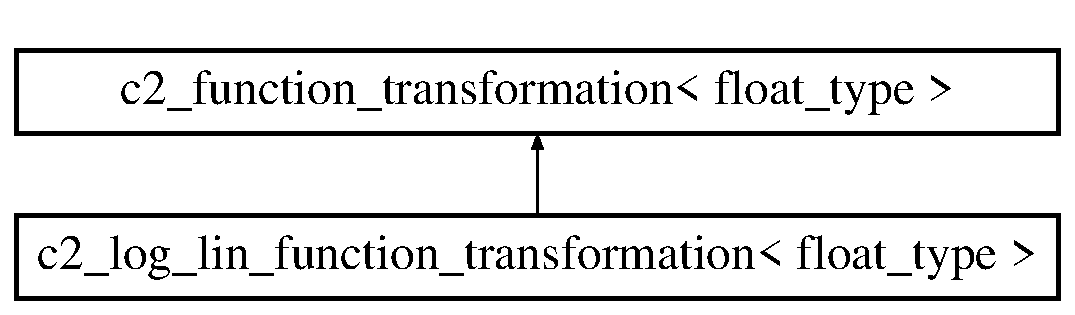
\includegraphics[height=2.000000cm]{classc2__log__lin__function__transformation}
\end{center}
\end{figure}
\subsection*{Additional Inherited Members}


\subsection{Detailed Description}
\subsubsection*{template$<$typename float\-\_\-type$>$class c2\-\_\-log\-\_\-lin\-\_\-function\-\_\-transformation$<$ float\-\_\-type $>$}

a transformation of a function in and out of log-\/lin space 



The documentation for this class was generated from the following file\-:\begin{DoxyCompactItemize}
\item 
\hyperlink{c2__function_8hh}{c2\-\_\-function.\-hh}\end{DoxyCompactItemize}

\hypertarget{classc2__log__log__function__transformation}{\section{c2\-\_\-log\-\_\-log\-\_\-function\-\_\-transformation$<$ float\-\_\-type $>$ Class Template Reference}
\label{classc2__log__log__function__transformation}\index{c2\-\_\-log\-\_\-log\-\_\-function\-\_\-transformation$<$ float\-\_\-type $>$@{c2\-\_\-log\-\_\-log\-\_\-function\-\_\-transformation$<$ float\-\_\-type $>$}}
}


a transformation of a function in and out of log-\/log space  




{\ttfamily \#include $<$c2\-\_\-function.\-hh$>$}

Inheritance diagram for c2\-\_\-log\-\_\-log\-\_\-function\-\_\-transformation$<$ float\-\_\-type $>$\-:\begin{figure}[H]
\begin{center}
\leavevmode
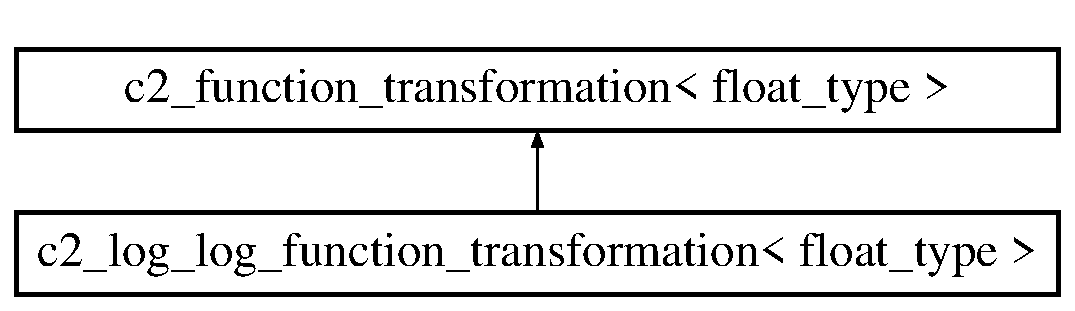
\includegraphics[height=2.000000cm]{classc2__log__log__function__transformation}
\end{center}
\end{figure}
\subsection*{Additional Inherited Members}


\subsection{Detailed Description}
\subsubsection*{template$<$typename float\-\_\-type$>$class c2\-\_\-log\-\_\-log\-\_\-function\-\_\-transformation$<$ float\-\_\-type $>$}

a transformation of a function in and out of log-\/log space 



The documentation for this class was generated from the following file\-:\begin{DoxyCompactItemize}
\item 
\hyperlink{c2__function_8hh}{c2\-\_\-function.\-hh}\end{DoxyCompactItemize}

\hypertarget{classc2__log__p}{\section{c2\-\_\-log\-\_\-p$<$ float\-\_\-type $>$ Class Template Reference}
\label{classc2__log__p}\index{c2\-\_\-log\-\_\-p$<$ float\-\_\-type $>$@{c2\-\_\-log\-\_\-p$<$ float\-\_\-type $>$}}
}


compute log(x) with its derivatives.

The factory function \hyperlink{classc2__factory_af20c7c4fee421c8ee0b51bac1c42302e}{c2\-\_\-factory\-::log()} creates $\ast$new \hyperlink{classc2__log__p}{c2\-\_\-log\-\_\-p}  




{\ttfamily \#include $<$c2\-\_\-function.\-hh$>$}

Inheritance diagram for c2\-\_\-log\-\_\-p$<$ float\-\_\-type $>$\-:\begin{figure}[H]
\begin{center}
\leavevmode
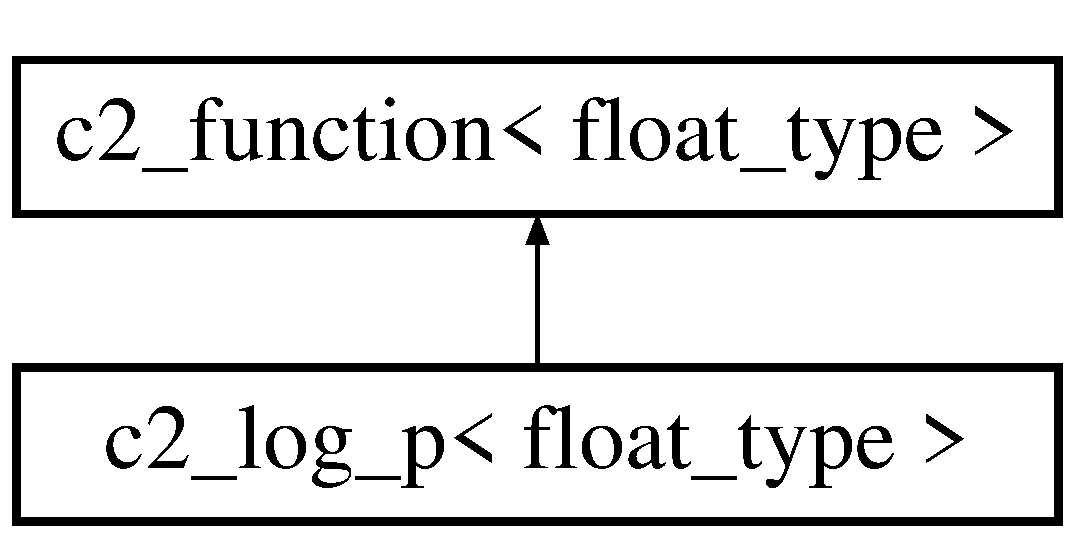
\includegraphics[height=2.000000cm]{classc2__log__p}
\end{center}
\end{figure}
\subsection*{Public Member Functions}
\begin{DoxyCompactItemize}
\item 
\hypertarget{classc2__log__p_a53da98f4d84ed9d95352b3b06f7a7a55}{\hyperlink{classc2__log__p_a53da98f4d84ed9d95352b3b06f7a7a55}{c2\-\_\-log\-\_\-p} ()}\label{classc2__log__p_a53da98f4d84ed9d95352b3b06f7a7a55}

\begin{DoxyCompactList}\small\item\em constructor. \end{DoxyCompactList}\item 
virtual float\-\_\-type \hyperlink{classc2__log__p_acd98067684930659e4a47390385e56b3}{value\-\_\-with\-\_\-derivatives} (float\-\_\-type x, float\-\_\-type $\ast$yprime, float\-\_\-type $\ast$yprime2) const   throw (c2\-\_\-exception)
\begin{DoxyCompactList}\small\item\em get the value and derivatives. \end{DoxyCompactList}\end{DoxyCompactItemize}
\subsection*{Additional Inherited Members}


\subsection{Detailed Description}
\subsubsection*{template$<$typename float\-\_\-type = double$>$class c2\-\_\-log\-\_\-p$<$ float\-\_\-type $>$}

compute log(x) with its derivatives.

The factory function \hyperlink{classc2__factory_af20c7c4fee421c8ee0b51bac1c42302e}{c2\-\_\-factory\-::log()} creates $\ast$new \hyperlink{classc2__log__p}{c2\-\_\-log\-\_\-p} 

\subsection{Member Function Documentation}
\hypertarget{classc2__log__p_acd98067684930659e4a47390385e56b3}{\index{c2\-\_\-log\-\_\-p@{c2\-\_\-log\-\_\-p}!value\-\_\-with\-\_\-derivatives@{value\-\_\-with\-\_\-derivatives}}
\index{value\-\_\-with\-\_\-derivatives@{value\-\_\-with\-\_\-derivatives}!c2_log_p@{c2\-\_\-log\-\_\-p}}
\subsubsection[{value\-\_\-with\-\_\-derivatives}]{\setlength{\rightskip}{0pt plus 5cm}template$<$typename float\-\_\-type  = double$>$ virtual float\-\_\-type {\bf c2\-\_\-log\-\_\-p}$<$ float\-\_\-type $>$\-::value\-\_\-with\-\_\-derivatives (
\begin{DoxyParamCaption}
\item[{float\-\_\-type}]{x, }
\item[{float\-\_\-type $\ast$}]{yprime, }
\item[{float\-\_\-type $\ast$}]{yprime2}
\end{DoxyParamCaption}
) const throw  {\bf c2\-\_\-exception}) \hspace{0.3cm}{\ttfamily [inline]}, {\ttfamily [virtual]}}}\label{classc2__log__p_acd98067684930659e4a47390385e56b3}


get the value and derivatives. 

There is required checking for null pointers on the derivatives, and most implementations should operate faster if derivatives are not needed. 
\begin{DoxyParams}[1]{Parameters}
\mbox{\tt in}  & {\em x} & the point at which to evaluate the function \\
\hline
\mbox{\tt out}  & {\em yprime} & the first derivative (if pointer is non-\/null) \\
\hline
\mbox{\tt out}  & {\em yprime2} & the second derivative (if pointer is non-\/null) \\
\hline
\end{DoxyParams}
\begin{DoxyReturn}{Returns}
the value of the function 
\end{DoxyReturn}


Implements \hyperlink{classc2__function_a44e0201159111350be7f746fc9026f67}{c2\-\_\-function$<$ float\-\_\-type $>$}.



The documentation for this class was generated from the following file\-:\begin{DoxyCompactItemize}
\item 
\hyperlink{c2__function_8hh}{c2\-\_\-function.\-hh}\end{DoxyCompactItemize}

\hypertarget{classc2__piecewise__function__p}{}\section{c2\+\_\+piecewise\+\_\+function\+\_\+p$<$ float\+\_\+type $>$ Class Template Reference}
\label{classc2__piecewise__function__p}\index{c2\+\_\+piecewise\+\_\+function\+\_\+p$<$ float\+\_\+type $>$@{c2\+\_\+piecewise\+\_\+function\+\_\+p$<$ float\+\_\+type $>$}}


create a \hyperlink{classc2__function}{c2\+\_\+function} which is a piecewise assembly of other c2\+\_\+functions.

The functions must have increasing, non-\/overlapping domains. Any empty space between functions will be filled with a linear interpolation.  




{\ttfamily \#include \char`\"{}c2\+\_\+function.\+hh\char`\"{}}



Inheritance diagram for c2\+\_\+piecewise\+\_\+function\+\_\+p$<$ float\+\_\+type $>$\+:
\nopagebreak
\begin{figure}[H]
\begin{center}
\leavevmode
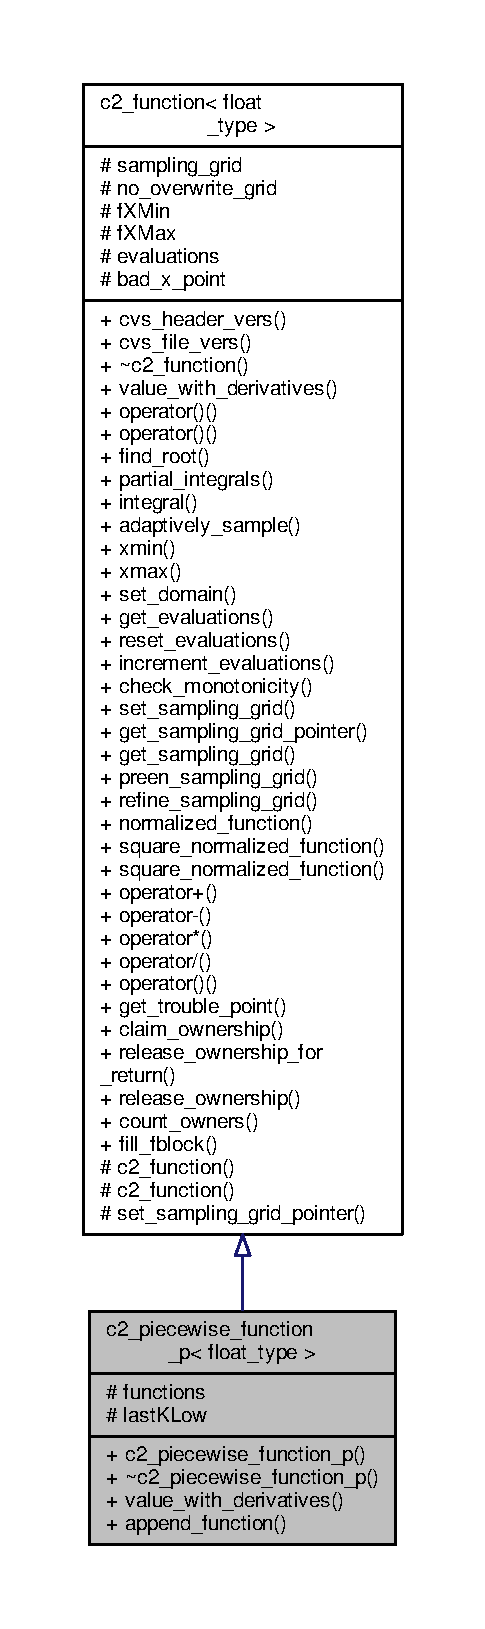
\includegraphics[height=550pt]{classc2__piecewise__function__p__inherit__graph}
\end{center}
\end{figure}


Collaboration diagram for c2\+\_\+piecewise\+\_\+function\+\_\+p$<$ float\+\_\+type $>$\+:
\nopagebreak
\begin{figure}[H]
\begin{center}
\leavevmode
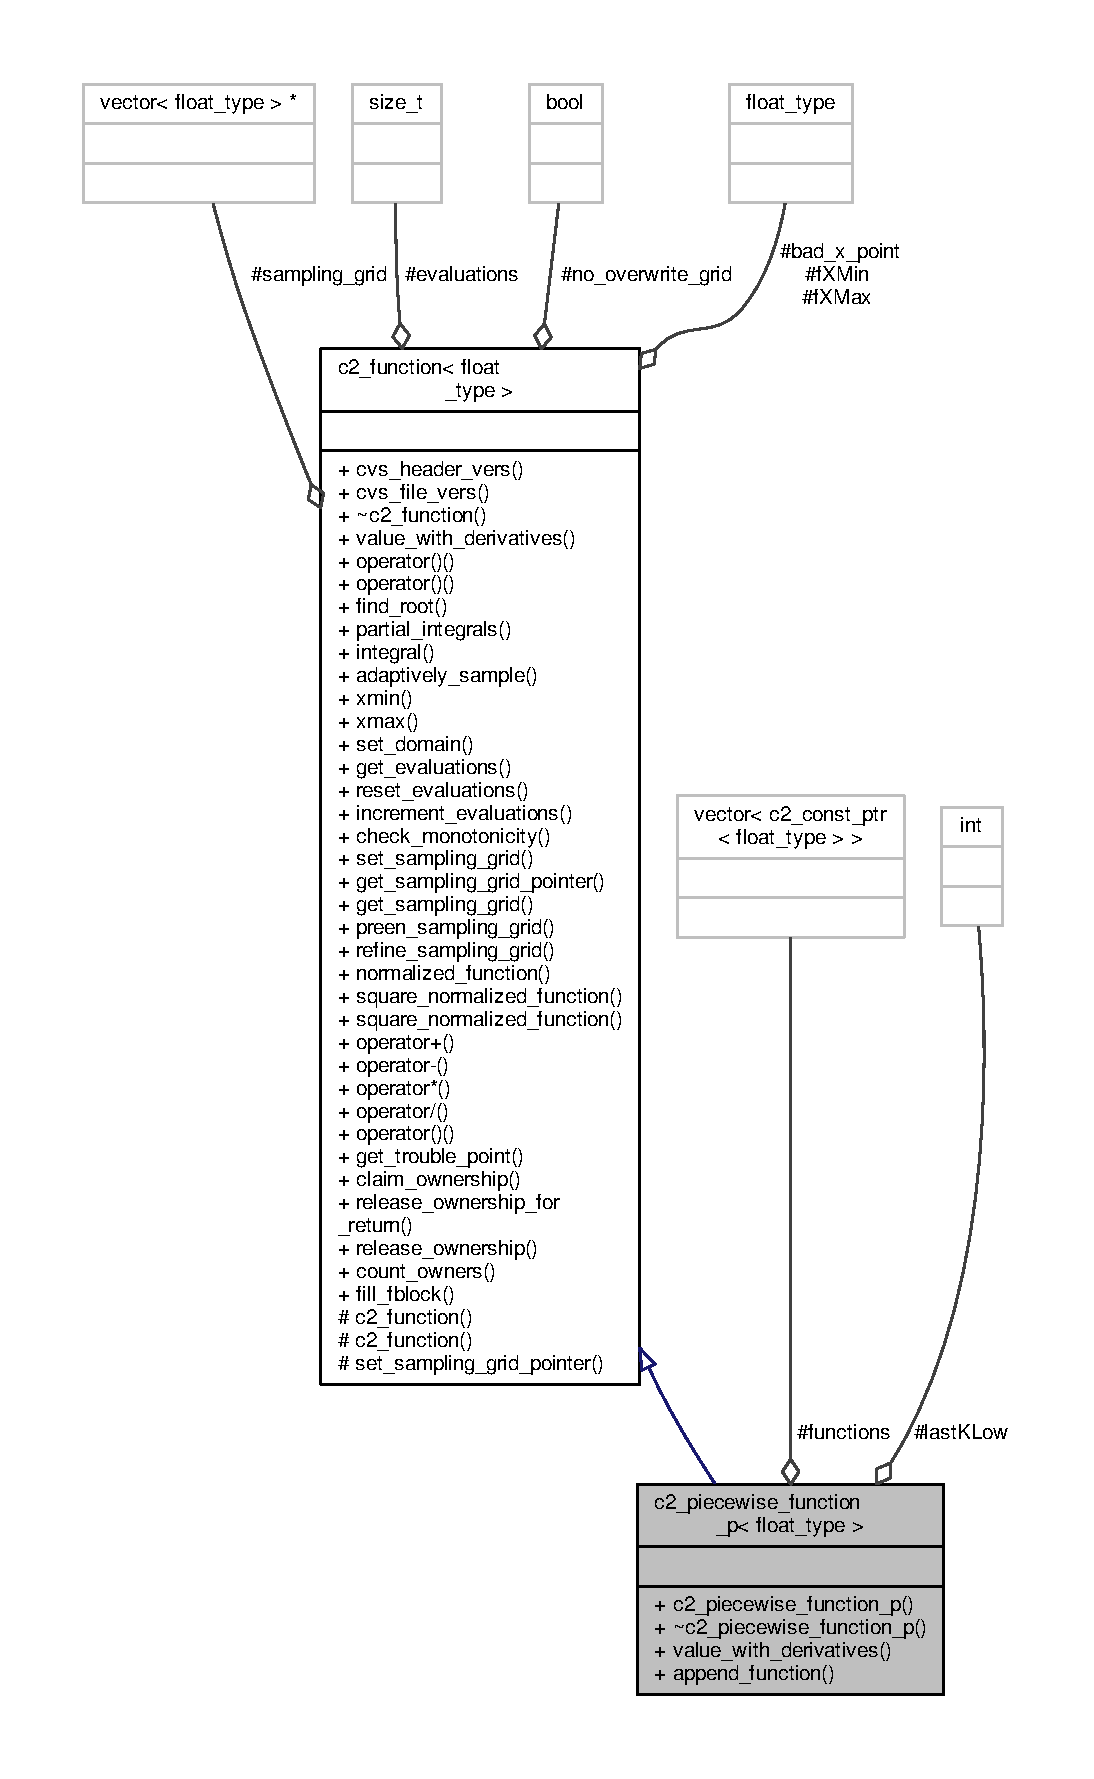
\includegraphics[height=550pt]{classc2__piecewise__function__p__coll__graph}
\end{center}
\end{figure}
\subsection*{Public Member Functions}
\begin{DoxyCompactItemize}
\item 
\hyperlink{classc2__piecewise__function__p_af97c8865a492b191be0d25146efd17e0}{c2\+\_\+piecewise\+\_\+function\+\_\+p} ()
\begin{DoxyCompactList}\small\item\em construct the container \end{DoxyCompactList}\item 
virtual \hyperlink{classc2__piecewise__function__p_ae4568a15bc298e69a25d1b05a25a3c1f}{$\sim$c2\+\_\+piecewise\+\_\+function\+\_\+p} ()
\begin{DoxyCompactList}\small\item\em destructor \end{DoxyCompactList}\item 
virtual float\+\_\+type \hyperlink{classc2__piecewise__function__p_a24dda73e84778fa9eb2160195403c45f}{value\+\_\+with\+\_\+derivatives} (float\+\_\+type x, float\+\_\+type $\ast$yprime, float\+\_\+type $\ast$yprime2) const   throw (c2\+\_\+exception)
\begin{DoxyCompactList}\small\item\em get the value and derivatives. \end{DoxyCompactList}\item 
void \hyperlink{classc2__piecewise__function__p_accaab7a03beef73ee88d6cfed30f52df}{append\+\_\+function} (const \hyperlink{classc2__function}{c2\+\_\+function}$<$ float\+\_\+type $>$ \&func)  throw (c2\+\_\+exception)
\begin{DoxyCompactList}\small\item\em append a new function to the sequence \end{DoxyCompactList}\end{DoxyCompactItemize}
\subsection*{Protected Attributes}
\begin{DoxyCompactItemize}
\item 
std\+::vector$<$ \hyperlink{classc2__const__ptr}{c2\+\_\+const\+\_\+ptr}$<$ float\+\_\+type $>$ $>$ \hyperlink{classc2__piecewise__function__p_aa408053c36b9fa349a5ea9b0b4badc0d}{functions}
\item 
int \hyperlink{classc2__piecewise__function__p_a8231d5c512db23c48712b7cba0ea0bca}{last\+K\+Low}
\end{DoxyCompactItemize}
\subsection*{Additional Inherited Members}


\subsection{Detailed Description}
\subsubsection*{template$<$typename float\+\_\+type = double$>$\\*
class c2\+\_\+piecewise\+\_\+function\+\_\+p$<$ float\+\_\+type $>$}

create a \hyperlink{classc2__function}{c2\+\_\+function} which is a piecewise assembly of other c2\+\_\+functions.

The functions must have increasing, non-\/overlapping domains. Any empty space between functions will be filled with a linear interpolation. 

\begin{DoxyNote}{Note}
If you want a smooth connection, instead of the default linear interpolation, create a \hyperlink{classc2__connector__function__p}{c2\+\_\+connector\+\_\+function\+\_\+p} to bridge the gap. The linear interpolation is intended to be a barely intelligent bridge, and may never get used by anyone.

The creation of the container results in the creation of an explicit sampling grid. If this is used with functions with a large domain, or which generate very dense sampling grids, it could eat a lot of memory. Do not abuse this by using functions which can generate gigantic grids.
\end{DoxyNote}
\begin{DoxySeeAlso}{See also}
Sample Applications ~\newline
\hyperlink{classc2__plugin__function__p}{c2\+\_\+plugin\+\_\+function\+\_\+p} page ~\newline
\hyperlink{classc2__connector__function__p}{c2\+\_\+connector\+\_\+function\+\_\+p} page ~\newline
\hyperlink{classc2__function_aea75f73d6a97087571c163ae4e514652}{Adaptive sampling}
\end{DoxySeeAlso}
The factory function \hyperlink{classc2__factory_ae8073f403ae804870d8ce71e67175507}{c2\+\_\+factory\+::piecewise\+\_\+function()} creates $\ast$new \hyperlink{classc2__piecewise__function__p}{c2\+\_\+piecewise\+\_\+function\+\_\+p} 

\subsection{Constructor \& Destructor Documentation}
\index{c2\+\_\+piecewise\+\_\+function\+\_\+p@{c2\+\_\+piecewise\+\_\+function\+\_\+p}!c2\+\_\+piecewise\+\_\+function\+\_\+p@{c2\+\_\+piecewise\+\_\+function\+\_\+p}}
\index{c2\+\_\+piecewise\+\_\+function\+\_\+p@{c2\+\_\+piecewise\+\_\+function\+\_\+p}!c2\+\_\+piecewise\+\_\+function\+\_\+p@{c2\+\_\+piecewise\+\_\+function\+\_\+p}}
\subsubsection[{\texorpdfstring{c2\+\_\+piecewise\+\_\+function\+\_\+p()}{c2_piecewise_function_p()}}]{\setlength{\rightskip}{0pt plus 5cm}template$<$typename float\+\_\+type = double$>$ {\bf c2\+\_\+piecewise\+\_\+function\+\_\+p}$<$ float\+\_\+type $>$\+::{\bf c2\+\_\+piecewise\+\_\+function\+\_\+p} (
\begin{DoxyParamCaption}
{}
\end{DoxyParamCaption}
)}\hypertarget{classc2__piecewise__function__p_af97c8865a492b191be0d25146efd17e0}{}\label{classc2__piecewise__function__p_af97c8865a492b191be0d25146efd17e0}


construct the container 

\index{c2\+\_\+piecewise\+\_\+function\+\_\+p@{c2\+\_\+piecewise\+\_\+function\+\_\+p}!````~c2\+\_\+piecewise\+\_\+function\+\_\+p@{$\sim$c2\+\_\+piecewise\+\_\+function\+\_\+p}}
\index{````~c2\+\_\+piecewise\+\_\+function\+\_\+p@{$\sim$c2\+\_\+piecewise\+\_\+function\+\_\+p}!c2\+\_\+piecewise\+\_\+function\+\_\+p@{c2\+\_\+piecewise\+\_\+function\+\_\+p}}
\subsubsection[{\texorpdfstring{$\sim$c2\+\_\+piecewise\+\_\+function\+\_\+p()}{~c2_piecewise_function_p()}}]{\setlength{\rightskip}{0pt plus 5cm}template$<$typename float\+\_\+type = double$>$ virtual {\bf c2\+\_\+piecewise\+\_\+function\+\_\+p}$<$ float\+\_\+type $>$\+::$\sim${\bf c2\+\_\+piecewise\+\_\+function\+\_\+p} (
\begin{DoxyParamCaption}
{}
\end{DoxyParamCaption}
)\hspace{0.3cm}{\ttfamily [virtual]}}\hypertarget{classc2__piecewise__function__p_ae4568a15bc298e69a25d1b05a25a3c1f}{}\label{classc2__piecewise__function__p_ae4568a15bc298e69a25d1b05a25a3c1f}


destructor 



\subsection{Member Function Documentation}
\index{c2\+\_\+piecewise\+\_\+function\+\_\+p@{c2\+\_\+piecewise\+\_\+function\+\_\+p}!append\+\_\+function@{append\+\_\+function}}
\index{append\+\_\+function@{append\+\_\+function}!c2\+\_\+piecewise\+\_\+function\+\_\+p@{c2\+\_\+piecewise\+\_\+function\+\_\+p}}
\subsubsection[{\texorpdfstring{append\+\_\+function(const c2\+\_\+function$<$ float\+\_\+type $>$ \&func)}{append_function(const c2_function< float_type > &func)}}]{\setlength{\rightskip}{0pt plus 5cm}template$<$typename float\+\_\+type = double$>$ void {\bf c2\+\_\+piecewise\+\_\+function\+\_\+p}$<$ float\+\_\+type $>$\+::append\+\_\+function (
\begin{DoxyParamCaption}
\item[{const {\bf c2\+\_\+function}$<$ float\+\_\+type $>$ \&}]{func}
\end{DoxyParamCaption}
) throw  {\bf c2\+\_\+exception}) }\hypertarget{classc2__piecewise__function__p_accaab7a03beef73ee88d6cfed30f52df}{}\label{classc2__piecewise__function__p_accaab7a03beef73ee88d6cfed30f52df}


append a new function to the sequence 

This takes a \hyperlink{classc2__function}{c2\+\_\+function}, and appends it onto the end of the piecewise collection. The domain of the function (which M\+U\+ST be set) specifies the place it will be used in the final function. If the domain exactly abuts the domain of the previous function, it will be directly attached. If there is a gap, the gap will be filled in by linear interpolation. 
\begin{DoxyParams}{Parameters}
{\em func} & a \hyperlink{classc2__function}{c2\+\_\+function} with a defined domain to be appended to the collection \\
\hline
\end{DoxyParams}
\index{c2\+\_\+piecewise\+\_\+function\+\_\+p@{c2\+\_\+piecewise\+\_\+function\+\_\+p}!value\+\_\+with\+\_\+derivatives@{value\+\_\+with\+\_\+derivatives}}
\index{value\+\_\+with\+\_\+derivatives@{value\+\_\+with\+\_\+derivatives}!c2\+\_\+piecewise\+\_\+function\+\_\+p@{c2\+\_\+piecewise\+\_\+function\+\_\+p}}
\subsubsection[{\texorpdfstring{value\+\_\+with\+\_\+derivatives(float\+\_\+type x, float\+\_\+type $\ast$yprime, float\+\_\+type $\ast$yprime2) const }{value_with_derivatives(float_type x, float_type *yprime, float_type *yprime2) const }}]{\setlength{\rightskip}{0pt plus 5cm}template$<$typename float\+\_\+type = double$>$ virtual float\+\_\+type {\bf c2\+\_\+piecewise\+\_\+function\+\_\+p}$<$ float\+\_\+type $>$\+::value\+\_\+with\+\_\+derivatives (
\begin{DoxyParamCaption}
\item[{float\+\_\+type}]{x, }
\item[{float\+\_\+type $\ast$}]{yprime, }
\item[{float\+\_\+type $\ast$}]{yprime2}
\end{DoxyParamCaption}
) const throw  {\bf c2\+\_\+exception}) \hspace{0.3cm}{\ttfamily [virtual]}}\hypertarget{classc2__piecewise__function__p_a24dda73e84778fa9eb2160195403c45f}{}\label{classc2__piecewise__function__p_a24dda73e84778fa9eb2160195403c45f}


get the value and derivatives. 

There is required checking for null pointers on the derivatives, and most implementations should operate faster if derivatives are not needed. 
\begin{DoxyParams}[1]{Parameters}
\mbox{\tt in}  & {\em x} & the point at which to evaluate the function \\
\hline
\mbox{\tt out}  & {\em yprime} & the first derivative (if pointer is non-\/null) \\
\hline
\mbox{\tt out}  & {\em yprime2} & the second derivative (if pointer is non-\/null) \\
\hline
\end{DoxyParams}
\begin{DoxyReturn}{Returns}
the value of the function 
\end{DoxyReturn}


Implements \hyperlink{classc2__function_a44e0201159111350be7f746fc9026f67}{c2\+\_\+function$<$ float\+\_\+type $>$}.



\subsection{Member Data Documentation}
\index{c2\+\_\+piecewise\+\_\+function\+\_\+p@{c2\+\_\+piecewise\+\_\+function\+\_\+p}!functions@{functions}}
\index{functions@{functions}!c2\+\_\+piecewise\+\_\+function\+\_\+p@{c2\+\_\+piecewise\+\_\+function\+\_\+p}}
\subsubsection[{\texorpdfstring{functions}{functions}}]{\setlength{\rightskip}{0pt plus 5cm}template$<$typename float\+\_\+type = double$>$ std\+::vector$<${\bf c2\+\_\+const\+\_\+ptr}$<$float\+\_\+type$>$ $>$ {\bf c2\+\_\+piecewise\+\_\+function\+\_\+p}$<$ float\+\_\+type $>$\+::functions\hspace{0.3cm}{\ttfamily [protected]}}\hypertarget{classc2__piecewise__function__p_aa408053c36b9fa349a5ea9b0b4badc0d}{}\label{classc2__piecewise__function__p_aa408053c36b9fa349a5ea9b0b4badc0d}
\index{c2\+\_\+piecewise\+\_\+function\+\_\+p@{c2\+\_\+piecewise\+\_\+function\+\_\+p}!last\+K\+Low@{last\+K\+Low}}
\index{last\+K\+Low@{last\+K\+Low}!c2\+\_\+piecewise\+\_\+function\+\_\+p@{c2\+\_\+piecewise\+\_\+function\+\_\+p}}
\subsubsection[{\texorpdfstring{last\+K\+Low}{lastKLow}}]{\setlength{\rightskip}{0pt plus 5cm}template$<$typename float\+\_\+type = double$>$ int {\bf c2\+\_\+piecewise\+\_\+function\+\_\+p}$<$ float\+\_\+type $>$\+::last\+K\+Low\hspace{0.3cm}{\ttfamily [mutable]}, {\ttfamily [protected]}}\hypertarget{classc2__piecewise__function__p_a8231d5c512db23c48712b7cba0ea0bca}{}\label{classc2__piecewise__function__p_a8231d5c512db23c48712b7cba0ea0bca}


The documentation for this class was generated from the following file\+:\begin{DoxyCompactItemize}
\item 
\hyperlink{c2__function_8hh}{c2\+\_\+function.\+hh}\end{DoxyCompactItemize}

\hypertarget{classc2__plugin__function__p}{\section{c2\-\_\-plugin\-\_\-function\-\_\-p$<$ float\-\_\-type $>$ Class Template Reference}
\label{classc2__plugin__function__p}\index{c2\-\_\-plugin\-\_\-function\-\_\-p$<$ float\-\_\-type $>$@{c2\-\_\-plugin\-\_\-function\-\_\-p$<$ float\-\_\-type $>$}}
}


a container into which any other \hyperlink{classc2__function}{c2\-\_\-function} can be dropped, to allow expressions with replacable components.

It is useful for plugging different Interpolating\-Functions into a \hyperlink{classc2__function}{c2\-\_\-function} expression. It saves a lot of effort in other places with casting away const declarations.  




{\ttfamily \#include $<$c2\-\_\-function.\-hh$>$}

Inheritance diagram for c2\-\_\-plugin\-\_\-function\-\_\-p$<$ float\-\_\-type $>$\-:\begin{figure}[H]
\begin{center}
\leavevmode
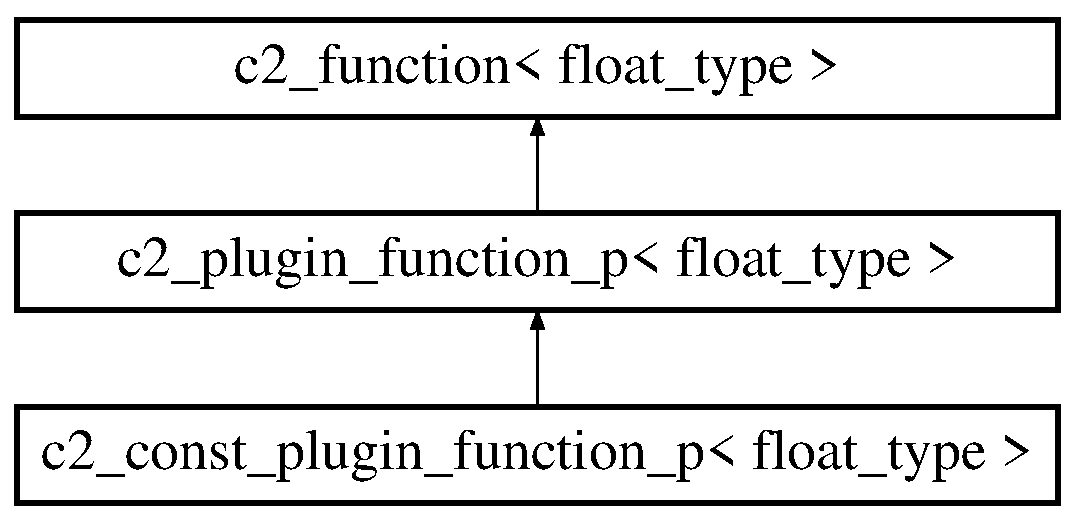
\includegraphics[height=3.000000cm]{classc2__plugin__function__p}
\end{center}
\end{figure}
\subsection*{Public Member Functions}
\begin{DoxyCompactItemize}
\item 
\hypertarget{classc2__plugin__function__p_aead9e593b067ffcb7387b350db7ea920}{\hyperlink{classc2__plugin__function__p_aead9e593b067ffcb7387b350db7ea920}{c2\-\_\-plugin\-\_\-function\-\_\-p} ()}\label{classc2__plugin__function__p_aead9e593b067ffcb7387b350db7ea920}

\begin{DoxyCompactList}\small\item\em construct the container with no function \end{DoxyCompactList}\item 
\hypertarget{classc2__plugin__function__p_a6b2825f01dffa6eaf84f7d4355a97f03}{\hyperlink{classc2__plugin__function__p_a6b2825f01dffa6eaf84f7d4355a97f03}{c2\-\_\-plugin\-\_\-function\-\_\-p} (\hyperlink{classc2__function}{c2\-\_\-function}$<$ float\-\_\-type $>$ \&f)}\label{classc2__plugin__function__p_a6b2825f01dffa6eaf84f7d4355a97f03}

\begin{DoxyCompactList}\small\item\em construct the container with a pre-\/defined function \end{DoxyCompactList}\item 
\hypertarget{classc2__plugin__function__p_a5d06682ac3e78308631700b1cde961ef}{void \hyperlink{classc2__plugin__function__p_a5d06682ac3e78308631700b1cde961ef}{set\-\_\-function} (\hyperlink{classc2__function}{c2\-\_\-function}$<$ float\-\_\-type $>$ $\ast$f)}\label{classc2__plugin__function__p_a5d06682ac3e78308631700b1cde961ef}

\begin{DoxyCompactList}\small\item\em fill the container with a new function, or clear it with a null pointer and copy our domain \end{DoxyCompactList}\item 
virtual float\-\_\-type \hyperlink{classc2__plugin__function__p_a7a5f8926ecec5b73f32ad5f90cefe80e}{value\-\_\-with\-\_\-derivatives} (float\-\_\-type x, float\-\_\-type $\ast$yprime, float\-\_\-type $\ast$yprime2) const   throw (c2\-\_\-exception)
\begin{DoxyCompactList}\small\item\em get the value and derivatives. \end{DoxyCompactList}\item 
\hypertarget{classc2__plugin__function__p_aac74d9e2221ee6b8fee5adc579960530}{virtual \hyperlink{classc2__plugin__function__p_aac74d9e2221ee6b8fee5adc579960530}{$\sim$c2\-\_\-plugin\-\_\-function\-\_\-p} ()}\label{classc2__plugin__function__p_aac74d9e2221ee6b8fee5adc579960530}

\begin{DoxyCompactList}\small\item\em destructor \end{DoxyCompactList}\item 
\hypertarget{classc2__plugin__function__p_aebe716e59908fe373f85e5aac964441f}{void \hyperlink{classc2__plugin__function__p_aebe716e59908fe373f85e5aac964441f}{unset\-\_\-function} ()}\label{classc2__plugin__function__p_aebe716e59908fe373f85e5aac964441f}

\begin{DoxyCompactList}\small\item\em clear our function \end{DoxyCompactList}\item 
virtual void \hyperlink{classc2__plugin__function__p_a0e7ff48329a648b3966efba72b15e3ed}{get\-\_\-sampling\-\_\-grid} (float\-\_\-type amin, float\-\_\-type amax, std\-::vector$<$ float\-\_\-type $>$ \&grid) const 
\begin{DoxyCompactList}\small\item\em return the grid of 'interesting' points along this function which lie in the region requested \end{DoxyCompactList}\end{DoxyCompactItemize}
\subsection*{Protected Attributes}
\begin{DoxyCompactItemize}
\item 
\hypertarget{classc2__plugin__function__p_a9f3ca0419f50aa9792da2a9b54716849}{\hyperlink{classc2__ptr}{c2\-\_\-ptr}$<$ float\-\_\-type $>$ {\bfseries func}}\label{classc2__plugin__function__p_a9f3ca0419f50aa9792da2a9b54716849}

\end{DoxyCompactItemize}
\subsection*{Additional Inherited Members}


\subsection{Detailed Description}
\subsubsection*{template$<$typename float\-\_\-type = double$>$class c2\-\_\-plugin\-\_\-function\-\_\-p$<$ float\-\_\-type $>$}

a container into which any other \hyperlink{classc2__function}{c2\-\_\-function} can be dropped, to allow expressions with replacable components.

It is useful for plugging different Interpolating\-Functions into a \hyperlink{classc2__function}{c2\-\_\-function} expression. It saves a lot of effort in other places with casting away const declarations. 

It is also useful as a wrapper for a function if it is necessary to have a copy of a function which has a different domain or sampling grid than the parent function. This can be be used, for example, to patch badly-\/behaved functions with \hyperlink{classc2__piecewise__function__p}{c2\-\_\-piecewise\-\_\-function\-\_\-p} by taking the parent function, creating two plugins of it with domains on each side of the nasty bit, and then inserting a nice function in the hole.

This can also be used as a fancier \hyperlink{classc2__ptr}{c2\-\_\-ptr} which allows direct evaluation instead of having to dereference the container first.

The factory function \hyperlink{classc2__factory_aaea82fa4f0b1f0183314a45923a3b673}{c2\-\_\-factory\-::plugin\-\_\-function()} creates $\ast$new \hyperlink{classc2__plugin__function__p_aead9e593b067ffcb7387b350db7ea920}{c2\-\_\-plugin\-\_\-function\-\_\-p()} 

\subsection{Member Function Documentation}
\hypertarget{classc2__plugin__function__p_a0e7ff48329a648b3966efba72b15e3ed}{\index{c2\-\_\-plugin\-\_\-function\-\_\-p@{c2\-\_\-plugin\-\_\-function\-\_\-p}!get\-\_\-sampling\-\_\-grid@{get\-\_\-sampling\-\_\-grid}}
\index{get\-\_\-sampling\-\_\-grid@{get\-\_\-sampling\-\_\-grid}!c2_plugin_function_p@{c2\-\_\-plugin\-\_\-function\-\_\-p}}
\subsubsection[{get\-\_\-sampling\-\_\-grid}]{\setlength{\rightskip}{0pt plus 5cm}template$<$typename float\-\_\-type = double$>$ virtual void {\bf c2\-\_\-plugin\-\_\-function\-\_\-p}$<$ float\-\_\-type $>$\-::get\-\_\-sampling\-\_\-grid (
\begin{DoxyParamCaption}
\item[{float\-\_\-type}]{amin, }
\item[{float\-\_\-type}]{amax, }
\item[{std\-::vector$<$ float\-\_\-type $>$ \&}]{grid}
\end{DoxyParamCaption}
) const\hspace{0.3cm}{\ttfamily [inline]}, {\ttfamily [virtual]}}}\label{classc2__plugin__function__p_a0e7ff48329a648b3966efba72b15e3ed}


return the grid of 'interesting' points along this function which lie in the region requested 

if a sampling grid is defined, work from there, otherwise return vector of (amin, amax) 
\begin{DoxyParams}[1]{Parameters}
 & {\em amin} & the lower bound for which the function is to be sampled \\
\hline
 & {\em amax} & the upper bound for which the function is to be sampled \\
\hline
\mbox{\tt in,out}  & {\em grid} & filled vector containing the samplng grid. \\
\hline
\end{DoxyParams}


Reimplemented from \hyperlink{classc2__function_ad03264dcc015e5d0b1b6eb30df3f32be}{c2\-\_\-function$<$ float\-\_\-type $>$}.

\hypertarget{classc2__plugin__function__p_a7a5f8926ecec5b73f32ad5f90cefe80e}{\index{c2\-\_\-plugin\-\_\-function\-\_\-p@{c2\-\_\-plugin\-\_\-function\-\_\-p}!value\-\_\-with\-\_\-derivatives@{value\-\_\-with\-\_\-derivatives}}
\index{value\-\_\-with\-\_\-derivatives@{value\-\_\-with\-\_\-derivatives}!c2_plugin_function_p@{c2\-\_\-plugin\-\_\-function\-\_\-p}}
\subsubsection[{value\-\_\-with\-\_\-derivatives}]{\setlength{\rightskip}{0pt plus 5cm}template$<$typename float\-\_\-type = double$>$ virtual float\-\_\-type {\bf c2\-\_\-plugin\-\_\-function\-\_\-p}$<$ float\-\_\-type $>$\-::value\-\_\-with\-\_\-derivatives (
\begin{DoxyParamCaption}
\item[{float\-\_\-type}]{x, }
\item[{float\-\_\-type $\ast$}]{yprime, }
\item[{float\-\_\-type $\ast$}]{yprime2}
\end{DoxyParamCaption}
) const throw  {\bf c2\-\_\-exception}) \hspace{0.3cm}{\ttfamily [inline]}, {\ttfamily [virtual]}}}\label{classc2__plugin__function__p_a7a5f8926ecec5b73f32ad5f90cefe80e}


get the value and derivatives. 

There is required checking for null pointers on the derivatives, and most implementations should operate faster if derivatives are not needed. 
\begin{DoxyParams}[1]{Parameters}
\mbox{\tt in}  & {\em x} & the point at which to evaluate the function \\
\hline
\mbox{\tt out}  & {\em yprime} & the first derivative (if pointer is non-\/null) \\
\hline
\mbox{\tt out}  & {\em yprime2} & the second derivative (if pointer is non-\/null) \\
\hline
\end{DoxyParams}
\begin{DoxyReturn}{Returns}
the value of the function Uses the internal function pointer set by \hyperlink{classc2__plugin__function__p_a5d06682ac3e78308631700b1cde961ef}{set\-\_\-function()}. 
\end{DoxyReturn}


Implements \hyperlink{classc2__function_a44e0201159111350be7f746fc9026f67}{c2\-\_\-function$<$ float\-\_\-type $>$}.



The documentation for this class was generated from the following file\-:\begin{DoxyCompactItemize}
\item 
\hyperlink{c2__function_8hh}{c2\-\_\-function.\-hh}\end{DoxyCompactItemize}

\hypertarget{classc2__power__law__p}{\section{c2\-\_\-power\-\_\-law\-\_\-p$<$ float\-\_\-type $>$ Class Template Reference}
\label{classc2__power__law__p}\index{c2\-\_\-power\-\_\-law\-\_\-p$<$ float\-\_\-type $>$@{c2\-\_\-power\-\_\-law\-\_\-p$<$ float\-\_\-type $>$}}
}


create a power law mapping of another function

for example, given a \hyperlink{classc2__function}{c2\-\_\-function} {\itshape f}  




{\ttfamily \#include $<$c2\-\_\-function.\-hh$>$}

Inheritance diagram for c2\-\_\-power\-\_\-law\-\_\-p$<$ float\-\_\-type $>$\-:\begin{figure}[H]
\begin{center}
\leavevmode
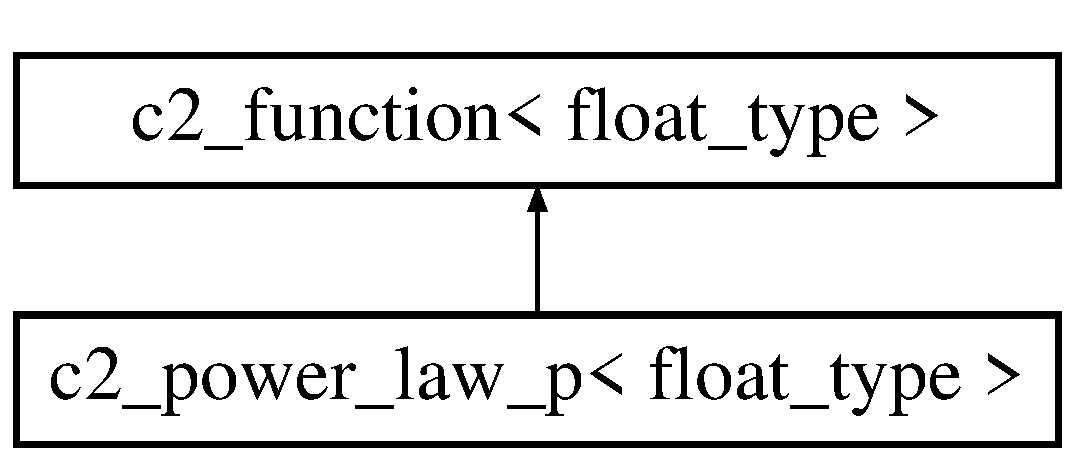
\includegraphics[height=2.000000cm]{classc2__power__law__p}
\end{center}
\end{figure}
\subsection*{Public Member Functions}
\begin{DoxyCompactItemize}
\item 
\hyperlink{classc2__power__law__p_aa94656e3e7b7fd9a78da1ff188258cc1}{c2\-\_\-power\-\_\-law\-\_\-p} (float\-\_\-type scale, float\-\_\-type power)
\begin{DoxyCompactList}\small\item\em Construct the operator. \end{DoxyCompactList}\item 
void \hyperlink{classc2__power__law__p_a2ac1227acd7b9bf34afd26efadc47ccb}{reset} (float\-\_\-type scale, float\-\_\-type power)
\begin{DoxyCompactList}\small\item\em Modify the mapping after construction. \end{DoxyCompactList}\item 
virtual float\-\_\-type \hyperlink{classc2__power__law__p_a21f0088450f7b7110a001f4960e95fa1}{value\-\_\-with\-\_\-derivatives} (float\-\_\-type x, float\-\_\-type $\ast$yprime, float\-\_\-type $\ast$yprime2) const   throw (c2\-\_\-exception)
\begin{DoxyCompactList}\small\item\em get the value and derivatives. \end{DoxyCompactList}\end{DoxyCompactItemize}
\subsection*{Additional Inherited Members}


\subsection{Detailed Description}
\subsubsection*{template$<$typename float\-\_\-type = double$>$class c2\-\_\-power\-\_\-law\-\_\-p$<$ float\-\_\-type $>$}

create a power law mapping of another function

for example, given a \hyperlink{classc2__function}{c2\-\_\-function} {\itshape f} 


\begin{DoxyCode}
\hyperlink{classc2__power__law__p}{c2\_power\_law\_p<double>} PLaw(1.2, 2.5);
\hyperlink{classc2__composed__function__p}{c2\_composed\_function\_p<double>} &F=PLaw(f); 
\end{DoxyCode}
 produces a new \hyperlink{classc2__function}{c2\-\_\-function} F=1.\-2 $\ast$ f$^\wedge$2.5

The factory function \hyperlink{classc2__factory_a2eb1ea80cc3c77555b519108cc0fad6b}{c2\-\_\-factory\-::power\-\_\-law()} creates $\ast$new \hyperlink{classc2__power__law__p}{c2\-\_\-power\-\_\-law\-\_\-p} 

\subsection{Constructor \& Destructor Documentation}
\hypertarget{classc2__power__law__p_aa94656e3e7b7fd9a78da1ff188258cc1}{\index{c2\-\_\-power\-\_\-law\-\_\-p@{c2\-\_\-power\-\_\-law\-\_\-p}!c2\-\_\-power\-\_\-law\-\_\-p@{c2\-\_\-power\-\_\-law\-\_\-p}}
\index{c2\-\_\-power\-\_\-law\-\_\-p@{c2\-\_\-power\-\_\-law\-\_\-p}!c2_power_law_p@{c2\-\_\-power\-\_\-law\-\_\-p}}
\subsubsection[{c2\-\_\-power\-\_\-law\-\_\-p}]{\setlength{\rightskip}{0pt plus 5cm}template$<$typename float\-\_\-type = double$>$ {\bf c2\-\_\-power\-\_\-law\-\_\-p}$<$ float\-\_\-type $>$\-::{\bf c2\-\_\-power\-\_\-law\-\_\-p} (
\begin{DoxyParamCaption}
\item[{float\-\_\-type}]{scale, }
\item[{float\-\_\-type}]{power}
\end{DoxyParamCaption}
)\hspace{0.3cm}{\ttfamily [inline]}}}\label{classc2__power__law__p_aa94656e3e7b7fd9a78da1ff188258cc1}


Construct the operator. 


\begin{DoxyParams}{Parameters}
{\em scale} & the multipler \\
\hline
{\em power} & the exponent \\
\hline
\end{DoxyParams}


\subsection{Member Function Documentation}
\hypertarget{classc2__power__law__p_a2ac1227acd7b9bf34afd26efadc47ccb}{\index{c2\-\_\-power\-\_\-law\-\_\-p@{c2\-\_\-power\-\_\-law\-\_\-p}!reset@{reset}}
\index{reset@{reset}!c2_power_law_p@{c2\-\_\-power\-\_\-law\-\_\-p}}
\subsubsection[{reset}]{\setlength{\rightskip}{0pt plus 5cm}template$<$typename float\-\_\-type = double$>$ void {\bf c2\-\_\-power\-\_\-law\-\_\-p}$<$ float\-\_\-type $>$\-::reset (
\begin{DoxyParamCaption}
\item[{float\-\_\-type}]{scale, }
\item[{float\-\_\-type}]{power}
\end{DoxyParamCaption}
)\hspace{0.3cm}{\ttfamily [inline]}}}\label{classc2__power__law__p_a2ac1227acd7b9bf34afd26efadc47ccb}


Modify the mapping after construction. 


\begin{DoxyParams}{Parameters}
{\em scale} & the new multipler \\
\hline
{\em power} & the new exponent \\
\hline
\end{DoxyParams}
\hypertarget{classc2__power__law__p_a21f0088450f7b7110a001f4960e95fa1}{\index{c2\-\_\-power\-\_\-law\-\_\-p@{c2\-\_\-power\-\_\-law\-\_\-p}!value\-\_\-with\-\_\-derivatives@{value\-\_\-with\-\_\-derivatives}}
\index{value\-\_\-with\-\_\-derivatives@{value\-\_\-with\-\_\-derivatives}!c2_power_law_p@{c2\-\_\-power\-\_\-law\-\_\-p}}
\subsubsection[{value\-\_\-with\-\_\-derivatives}]{\setlength{\rightskip}{0pt plus 5cm}template$<$typename float\-\_\-type = double$>$ virtual float\-\_\-type {\bf c2\-\_\-power\-\_\-law\-\_\-p}$<$ float\-\_\-type $>$\-::value\-\_\-with\-\_\-derivatives (
\begin{DoxyParamCaption}
\item[{float\-\_\-type}]{x, }
\item[{float\-\_\-type $\ast$}]{yprime, }
\item[{float\-\_\-type $\ast$}]{yprime2}
\end{DoxyParamCaption}
) const throw  {\bf c2\-\_\-exception}) \hspace{0.3cm}{\ttfamily [inline]}, {\ttfamily [virtual]}}}\label{classc2__power__law__p_a21f0088450f7b7110a001f4960e95fa1}


get the value and derivatives. 

There is required checking for null pointers on the derivatives, and most implementations should operate faster if derivatives are not needed. 
\begin{DoxyParams}[1]{Parameters}
\mbox{\tt in}  & {\em x} & the point at which to evaluate the function \\
\hline
\mbox{\tt out}  & {\em yprime} & the first derivative (if pointer is non-\/null) \\
\hline
\mbox{\tt out}  & {\em yprime2} & the second derivative (if pointer is non-\/null) \\
\hline
\end{DoxyParams}
\begin{DoxyReturn}{Returns}
the value of the function 
\end{DoxyReturn}


Implements \hyperlink{classc2__function_a44e0201159111350be7f746fc9026f67}{c2\-\_\-function$<$ float\-\_\-type $>$}.



The documentation for this class was generated from the following file\-:\begin{DoxyCompactItemize}
\item 
\hyperlink{c2__function_8hh}{c2\-\_\-function.\-hh}\end{DoxyCompactItemize}

\hypertarget{classc2__product__p}{}\section{c2\+\_\+product\+\_\+p$<$ float\+\_\+type $>$ Class Template Reference}
\label{classc2__product__p}\index{c2\+\_\+product\+\_\+p$<$ float\+\_\+type $>$@{c2\+\_\+product\+\_\+p$<$ float\+\_\+type $>$}}


create a \hyperlink{classc2__function}{c2\+\_\+function} which is the product of two other c2\+\_\+functions.

This should always be constructed using \hyperlink{classc2__function_a7744675c98a8ec63320ac1c0b61bec9c}{c2\+\_\+function\+::operator$\ast$()}  




{\ttfamily \#include \char`\"{}c2\+\_\+function.\+hh\char`\"{}}



Inheritance diagram for c2\+\_\+product\+\_\+p$<$ float\+\_\+type $>$\+:
\nopagebreak
\begin{figure}[H]
\begin{center}
\leavevmode
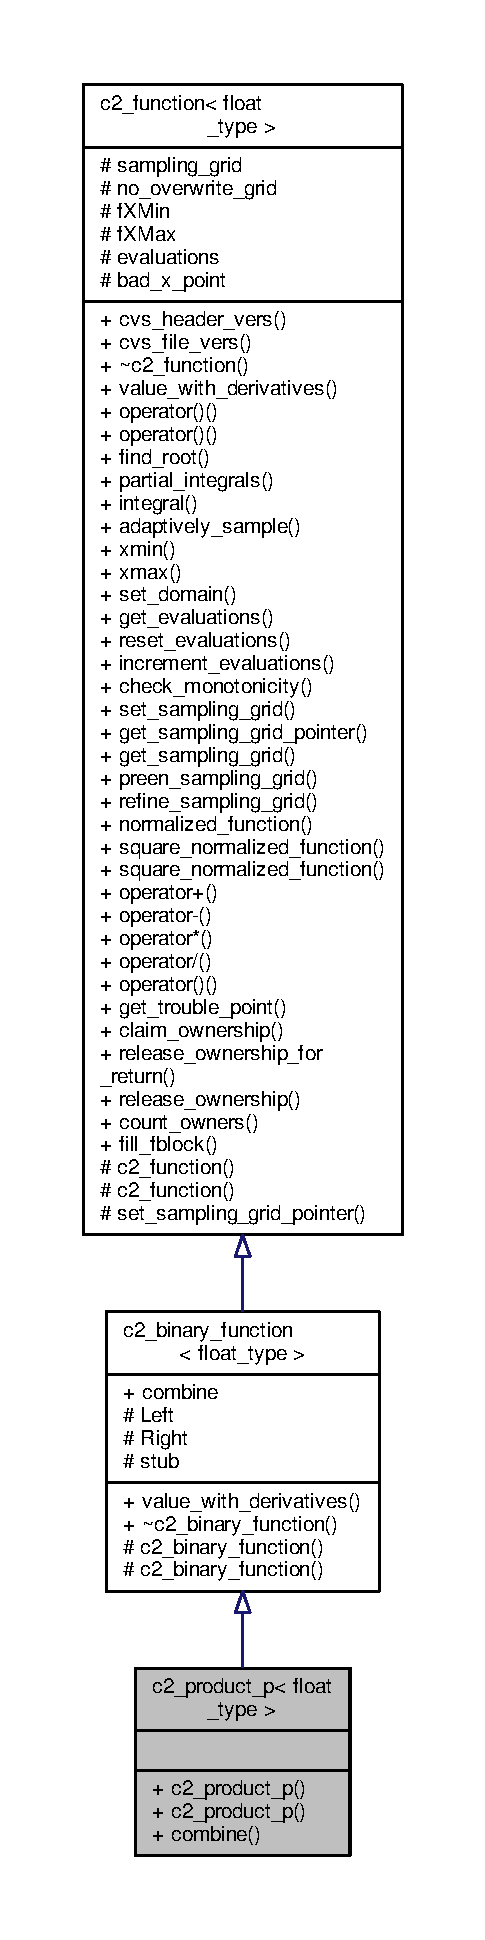
\includegraphics[height=550pt]{classc2__product__p__inherit__graph}
\end{center}
\end{figure}


Collaboration diagram for c2\+\_\+product\+\_\+p$<$ float\+\_\+type $>$\+:
\nopagebreak
\begin{figure}[H]
\begin{center}
\leavevmode
\includegraphics[width=350pt]{classc2__product__p__coll__graph}
\end{center}
\end{figure}
\subsection*{Public Member Functions}
\begin{DoxyCompactItemize}
\item 
\hyperlink{classc2__product__p_af39b700c5114f8e7fc46f12d23125fd8}{c2\+\_\+product\+\_\+p} (const \hyperlink{classc2__function}{c2\+\_\+function}$<$ float\+\_\+type $>$ \&left, const \hyperlink{classc2__function}{c2\+\_\+function}$<$ float\+\_\+type $>$ \&right)
\begin{DoxyCompactList}\small\item\em construct {\itshape left} $\ast$ {\itshape right} \end{DoxyCompactList}\item 
\hyperlink{classc2__product__p_a82b8eb1b1621b07a6a02ce38f3c2f40e}{c2\+\_\+product\+\_\+p} ()
\begin{DoxyCompactList}\small\item\em Create a stub just for the combiner to avoid statics. \end{DoxyCompactList}\end{DoxyCompactItemize}
\subsection*{Static Public Member Functions}
\begin{DoxyCompactItemize}
\item 
static float\+\_\+type \hyperlink{classc2__product__p_a35c37539a7ebc7074d5780a912dcb1d5}{combine} (const \hyperlink{classc2__function}{c2\+\_\+function}$<$ float\+\_\+type $>$ \&left, const \hyperlink{classc2__function}{c2\+\_\+function}$<$ float\+\_\+type $>$ \&right, float\+\_\+type x, float\+\_\+type $\ast$yprime, float\+\_\+type $\ast$yprime2)  throw (c2\+\_\+exception)
\begin{DoxyCompactList}\small\item\em execute math necessary to do multiplication \end{DoxyCompactList}\end{DoxyCompactItemize}
\subsection*{Additional Inherited Members}


\subsection{Detailed Description}
\subsubsection*{template$<$typename float\+\_\+type = double$>$\\*
class c2\+\_\+product\+\_\+p$<$ float\+\_\+type $>$}

create a \hyperlink{classc2__function}{c2\+\_\+function} which is the product of two other c2\+\_\+functions.

This should always be constructed using \hyperlink{classc2__function_a7744675c98a8ec63320ac1c0b61bec9c}{c2\+\_\+function\+::operator$\ast$()} 

\subsection{Constructor \& Destructor Documentation}
\index{c2\+\_\+product\+\_\+p@{c2\+\_\+product\+\_\+p}!c2\+\_\+product\+\_\+p@{c2\+\_\+product\+\_\+p}}
\index{c2\+\_\+product\+\_\+p@{c2\+\_\+product\+\_\+p}!c2\+\_\+product\+\_\+p@{c2\+\_\+product\+\_\+p}}
\subsubsection[{\texorpdfstring{c2\+\_\+product\+\_\+p(const c2\+\_\+function$<$ float\+\_\+type $>$ \&left, const c2\+\_\+function$<$ float\+\_\+type $>$ \&right)}{c2_product_p(const c2_function< float_type > &left, const c2_function< float_type > &right)}}]{\setlength{\rightskip}{0pt plus 5cm}template$<$typename float\+\_\+type  = double$>$ {\bf c2\+\_\+product\+\_\+p}$<$ float\+\_\+type $>$\+::{\bf c2\+\_\+product\+\_\+p} (
\begin{DoxyParamCaption}
\item[{const {\bf c2\+\_\+function}$<$ float\+\_\+type $>$ \&}]{left, }
\item[{const {\bf c2\+\_\+function}$<$ float\+\_\+type $>$ \&}]{right}
\end{DoxyParamCaption}
)\hspace{0.3cm}{\ttfamily [inline]}}\hypertarget{classc2__product__p_af39b700c5114f8e7fc46f12d23125fd8}{}\label{classc2__product__p_af39b700c5114f8e7fc46f12d23125fd8}


construct {\itshape left} $\ast$ {\itshape right} 


\begin{DoxyParams}{Parameters}
{\em left} & the left function \\
\hline
{\em right} & the right function \\
\hline
\end{DoxyParams}
\index{c2\+\_\+product\+\_\+p@{c2\+\_\+product\+\_\+p}!c2\+\_\+product\+\_\+p@{c2\+\_\+product\+\_\+p}}
\index{c2\+\_\+product\+\_\+p@{c2\+\_\+product\+\_\+p}!c2\+\_\+product\+\_\+p@{c2\+\_\+product\+\_\+p}}
\subsubsection[{\texorpdfstring{c2\+\_\+product\+\_\+p()}{c2_product_p()}}]{\setlength{\rightskip}{0pt plus 5cm}template$<$typename float\+\_\+type  = double$>$ {\bf c2\+\_\+product\+\_\+p}$<$ float\+\_\+type $>$\+::{\bf c2\+\_\+product\+\_\+p} (
\begin{DoxyParamCaption}
{}
\end{DoxyParamCaption}
)\hspace{0.3cm}{\ttfamily [inline]}}\hypertarget{classc2__product__p_a82b8eb1b1621b07a6a02ce38f3c2f40e}{}\label{classc2__product__p_a82b8eb1b1621b07a6a02ce38f3c2f40e}


Create a stub just for the combiner to avoid statics. 



\subsection{Member Function Documentation}
\index{c2\+\_\+product\+\_\+p@{c2\+\_\+product\+\_\+p}!combine@{combine}}
\index{combine@{combine}!c2\+\_\+product\+\_\+p@{c2\+\_\+product\+\_\+p}}
\subsubsection[{\texorpdfstring{combine(const c2\+\_\+function$<$ float\+\_\+type $>$ \&left, const c2\+\_\+function$<$ float\+\_\+type $>$ \&right, float\+\_\+type x, float\+\_\+type $\ast$yprime, float\+\_\+type $\ast$yprime2)}{combine(const c2_function< float_type > &left, const c2_function< float_type > &right, float_type x, float_type *yprime, float_type *yprime2)}}]{\setlength{\rightskip}{0pt plus 5cm}template$<$typename float\+\_\+type  = double$>$ static float\+\_\+type {\bf c2\+\_\+product\+\_\+p}$<$ float\+\_\+type $>$\+::combine (
\begin{DoxyParamCaption}
\item[{const {\bf c2\+\_\+function}$<$ float\+\_\+type $>$ \&}]{left, }
\item[{const {\bf c2\+\_\+function}$<$ float\+\_\+type $>$ \&}]{right, }
\item[{float\+\_\+type}]{x, }
\item[{float\+\_\+type $\ast$}]{yprime, }
\item[{float\+\_\+type $\ast$}]{yprime2}
\end{DoxyParamCaption}
) throw  {\bf c2\+\_\+exception}) \hspace{0.3cm}{\ttfamily [inline]}, {\ttfamily [static]}}\hypertarget{classc2__product__p_a35c37539a7ebc7074d5780a912dcb1d5}{}\label{classc2__product__p_a35c37539a7ebc7074d5780a912dcb1d5}


execute math necessary to do multiplication 



The documentation for this class was generated from the following file\+:\begin{DoxyCompactItemize}
\item 
\hyperlink{c2__function_8hh}{c2\+\_\+function.\+hh}\end{DoxyCompactItemize}

\hypertarget{classc2__ptr}{}\section{c2\+\_\+ptr$<$ float\+\_\+type $>$ Class Template Reference}
\label{classc2__ptr}\index{c2\+\_\+ptr$<$ float\+\_\+type $>$@{c2\+\_\+ptr$<$ float\+\_\+type $>$}}


create a container for a \hyperlink{classc2__function}{c2\+\_\+function} which handles the reference counting.  




{\ttfamily \#include \char`\"{}c2\+\_\+function.\+hh\char`\"{}}



Inheritance diagram for c2\+\_\+ptr$<$ float\+\_\+type $>$\+:
\nopagebreak
\begin{figure}[H]
\begin{center}
\leavevmode
\includegraphics[height=550pt]{classc2__ptr__inherit__graph}
\end{center}
\end{figure}


Collaboration diagram for c2\+\_\+ptr$<$ float\+\_\+type $>$\+:
\nopagebreak
\begin{figure}[H]
\begin{center}
\leavevmode
\includegraphics[height=550pt]{classc2__ptr__coll__graph}
\end{center}
\end{figure}
\subsection*{Public Member Functions}
\begin{DoxyCompactItemize}
\item 
\hyperlink{classc2__ptr_ad49d9f28b27b26366c125973f5f7a8c1}{c2\+\_\+ptr} ()
\begin{DoxyCompactList}\small\item\em construct the container with no function \end{DoxyCompactList}\item 
\hyperlink{classc2__ptr_a43bb3a5a3c7d65127a4782d305c45d15}{c2\+\_\+ptr} (\hyperlink{classc2__function}{c2\+\_\+function}$<$ float\+\_\+type $>$ \&f)
\begin{DoxyCompactList}\small\item\em construct the container with a pre-\/defined function \end{DoxyCompactList}\item 
\hyperlink{classc2__ptr_a0b3aa488bd5a4388048f574c2ef19e60}{c2\+\_\+ptr} (const \hyperlink{classc2__ptr}{c2\+\_\+ptr}$<$ float\+\_\+type $>$ \&src)
\begin{DoxyCompactList}\small\item\em copy constructor \end{DoxyCompactList}\item 
\hyperlink{classc2__function}{c2\+\_\+function}$<$ float\+\_\+type $>$ \& \hyperlink{classc2__ptr_afa91b91ad5c8c3479b02699afbb46d26}{get} () const   throw (c2\+\_\+exception)
\begin{DoxyCompactList}\small\item\em get a checked pointer to our owned function \end{DoxyCompactList}\item 
\hyperlink{classc2__function}{c2\+\_\+function}$<$ float\+\_\+type $>$ $\ast$ \hyperlink{classc2__ptr_a74378bfb73076c3d49156fdbfa063618}{get\+\_\+ptr} () const 
\begin{DoxyCompactList}\small\item\em get an unchecked pointer to our owned function \end{DoxyCompactList}\item 
\hyperlink{classc2__function}{c2\+\_\+function}$<$ float\+\_\+type $>$ $\ast$ \hyperlink{classc2__ptr_ade9595883ae73bfb22843c28045cb448}{operator-\/$>$} () const 
\begin{DoxyCompactList}\small\item\em get a checked pointer to our owned function \end{DoxyCompactList}\item 
const \hyperlink{classc2__ptr}{c2\+\_\+ptr}$<$ float\+\_\+type $>$ \& \hyperlink{classc2__ptr_ab176b3afe89de4456f3a4236cbf09008}{operator=} (const \hyperlink{classc2__ptr}{c2\+\_\+ptr}$<$ float\+\_\+type $>$ \&f)
\begin{DoxyCompactList}\small\item\em fill the container from another container \end{DoxyCompactList}\item 
\hyperlink{classc2__function}{c2\+\_\+function}$<$ float\+\_\+type $>$ \& \hyperlink{classc2__ptr_a7174f58864fa8e3439b6cfac256a1096}{operator=} (\hyperlink{classc2__function}{c2\+\_\+function}$<$ float\+\_\+type $>$ \&f)
\begin{DoxyCompactList}\small\item\em fill the container with a function \end{DoxyCompactList}\end{DoxyCompactItemize}
\subsection*{Additional Inherited Members}


\subsection{Detailed Description}
\subsubsection*{template$<$typename float\+\_\+type$>$\\*
class c2\+\_\+ptr$<$ float\+\_\+type $>$}

create a container for a \hyperlink{classc2__function}{c2\+\_\+function} which handles the reference counting. 

\begin{DoxySeeAlso}{See also}
\hyperlink{classc2__const__ptr}{c2\+\_\+const\+\_\+ptr} and Use of c2\+\_\+ptr for memory management 
\end{DoxySeeAlso}


\subsection{Constructor \& Destructor Documentation}
\index{c2\+\_\+ptr@{c2\+\_\+ptr}!c2\+\_\+ptr@{c2\+\_\+ptr}}
\index{c2\+\_\+ptr@{c2\+\_\+ptr}!c2\+\_\+ptr@{c2\+\_\+ptr}}
\subsubsection[{\texorpdfstring{c2\+\_\+ptr()}{c2_ptr()}}]{\setlength{\rightskip}{0pt plus 5cm}template$<$typename float\+\_\+type$>$ {\bf c2\+\_\+ptr}$<$ float\+\_\+type $>$\+::{\bf c2\+\_\+ptr} (
\begin{DoxyParamCaption}
{}
\end{DoxyParamCaption}
)\hspace{0.3cm}{\ttfamily [inline]}}\hypertarget{classc2__ptr_ad49d9f28b27b26366c125973f5f7a8c1}{}\label{classc2__ptr_ad49d9f28b27b26366c125973f5f7a8c1}


construct the container with no function 

\index{c2\+\_\+ptr@{c2\+\_\+ptr}!c2\+\_\+ptr@{c2\+\_\+ptr}}
\index{c2\+\_\+ptr@{c2\+\_\+ptr}!c2\+\_\+ptr@{c2\+\_\+ptr}}
\subsubsection[{\texorpdfstring{c2\+\_\+ptr(c2\+\_\+function$<$ float\+\_\+type $>$ \&f)}{c2_ptr(c2_function< float_type > &f)}}]{\setlength{\rightskip}{0pt plus 5cm}template$<$typename float\+\_\+type$>$ {\bf c2\+\_\+ptr}$<$ float\+\_\+type $>$\+::{\bf c2\+\_\+ptr} (
\begin{DoxyParamCaption}
\item[{{\bf c2\+\_\+function}$<$ float\+\_\+type $>$ \&}]{f}
\end{DoxyParamCaption}
)\hspace{0.3cm}{\ttfamily [inline]}}\hypertarget{classc2__ptr_a43bb3a5a3c7d65127a4782d305c45d15}{}\label{classc2__ptr_a43bb3a5a3c7d65127a4782d305c45d15}


construct the container with a pre-\/defined function 


\begin{DoxyParams}{Parameters}
{\em f} & the function to store \\
\hline
\end{DoxyParams}
\index{c2\+\_\+ptr@{c2\+\_\+ptr}!c2\+\_\+ptr@{c2\+\_\+ptr}}
\index{c2\+\_\+ptr@{c2\+\_\+ptr}!c2\+\_\+ptr@{c2\+\_\+ptr}}
\subsubsection[{\texorpdfstring{c2\+\_\+ptr(const c2\+\_\+ptr$<$ float\+\_\+type $>$ \&src)}{c2_ptr(const c2_ptr< float_type > &src)}}]{\setlength{\rightskip}{0pt plus 5cm}template$<$typename float\+\_\+type$>$ {\bf c2\+\_\+ptr}$<$ float\+\_\+type $>$\+::{\bf c2\+\_\+ptr} (
\begin{DoxyParamCaption}
\item[{const {\bf c2\+\_\+ptr}$<$ float\+\_\+type $>$ \&}]{src}
\end{DoxyParamCaption}
)\hspace{0.3cm}{\ttfamily [inline]}}\hypertarget{classc2__ptr_a0b3aa488bd5a4388048f574c2ef19e60}{}\label{classc2__ptr_a0b3aa488bd5a4388048f574c2ef19e60}


copy constructor 


\begin{DoxyParams}{Parameters}
{\em src} & the container to copy \\
\hline
\end{DoxyParams}


\subsection{Member Function Documentation}
\index{c2\+\_\+ptr@{c2\+\_\+ptr}!get@{get}}
\index{get@{get}!c2\+\_\+ptr@{c2\+\_\+ptr}}
\subsubsection[{\texorpdfstring{get() const }{get() const }}]{\setlength{\rightskip}{0pt plus 5cm}template$<$typename float\+\_\+type$>$ {\bf c2\+\_\+function}$<$float\+\_\+type$>$\& {\bf c2\+\_\+ptr}$<$ float\+\_\+type $>$\+::get (
\begin{DoxyParamCaption}
{}
\end{DoxyParamCaption}
) const throw  {\bf c2\+\_\+exception}) \hspace{0.3cm}{\ttfamily [inline]}}\hypertarget{classc2__ptr_afa91b91ad5c8c3479b02699afbb46d26}{}\label{classc2__ptr_afa91b91ad5c8c3479b02699afbb46d26}


get a checked pointer to our owned function 

\index{c2\+\_\+ptr@{c2\+\_\+ptr}!get\+\_\+ptr@{get\+\_\+ptr}}
\index{get\+\_\+ptr@{get\+\_\+ptr}!c2\+\_\+ptr@{c2\+\_\+ptr}}
\subsubsection[{\texorpdfstring{get\+\_\+ptr() const }{get_ptr() const }}]{\setlength{\rightskip}{0pt plus 5cm}template$<$typename float\+\_\+type$>$ {\bf c2\+\_\+function}$<$float\+\_\+type$>$$\ast$ {\bf c2\+\_\+ptr}$<$ float\+\_\+type $>$\+::get\+\_\+ptr (
\begin{DoxyParamCaption}
{}
\end{DoxyParamCaption}
) const\hspace{0.3cm}{\ttfamily [inline]}}\hypertarget{classc2__ptr_a74378bfb73076c3d49156fdbfa063618}{}\label{classc2__ptr_a74378bfb73076c3d49156fdbfa063618}


get an unchecked pointer to our owned function 

\index{c2\+\_\+ptr@{c2\+\_\+ptr}!operator-\/$>$@{operator-\/$>$}}
\index{operator-\/$>$@{operator-\/$>$}!c2\+\_\+ptr@{c2\+\_\+ptr}}
\subsubsection[{\texorpdfstring{operator-\/$>$() const }{operator->() const }}]{\setlength{\rightskip}{0pt plus 5cm}template$<$typename float\+\_\+type$>$ {\bf c2\+\_\+function}$<$float\+\_\+type$>$$\ast$ {\bf c2\+\_\+ptr}$<$ float\+\_\+type $>$\+::operator-\/$>$ (
\begin{DoxyParamCaption}
{}
\end{DoxyParamCaption}
) const\hspace{0.3cm}{\ttfamily [inline]}}\hypertarget{classc2__ptr_ade9595883ae73bfb22843c28045cb448}{}\label{classc2__ptr_ade9595883ae73bfb22843c28045cb448}


get a checked pointer to our owned function 

\index{c2\+\_\+ptr@{c2\+\_\+ptr}!operator=@{operator=}}
\index{operator=@{operator=}!c2\+\_\+ptr@{c2\+\_\+ptr}}
\subsubsection[{\texorpdfstring{operator=(const c2\+\_\+ptr$<$ float\+\_\+type $>$ \&f)}{operator=(const c2_ptr< float_type > &f)}}]{\setlength{\rightskip}{0pt plus 5cm}template$<$typename float\+\_\+type$>$ const {\bf c2\+\_\+ptr}$<$float\+\_\+type$>$\& {\bf c2\+\_\+ptr}$<$ float\+\_\+type $>$\+::operator= (
\begin{DoxyParamCaption}
\item[{const {\bf c2\+\_\+ptr}$<$ float\+\_\+type $>$ \&}]{f}
\end{DoxyParamCaption}
)\hspace{0.3cm}{\ttfamily [inline]}}\hypertarget{classc2__ptr_ab176b3afe89de4456f3a4236cbf09008}{}\label{classc2__ptr_ab176b3afe89de4456f3a4236cbf09008}


fill the container from another container 


\begin{DoxyParams}{Parameters}
{\em f} & the container to copy \\
\hline
\end{DoxyParams}
\index{c2\+\_\+ptr@{c2\+\_\+ptr}!operator=@{operator=}}
\index{operator=@{operator=}!c2\+\_\+ptr@{c2\+\_\+ptr}}
\subsubsection[{\texorpdfstring{operator=(c2\+\_\+function$<$ float\+\_\+type $>$ \&f)}{operator=(c2_function< float_type > &f)}}]{\setlength{\rightskip}{0pt plus 5cm}template$<$typename float\+\_\+type$>$ {\bf c2\+\_\+function}$<$float\+\_\+type$>$\& {\bf c2\+\_\+ptr}$<$ float\+\_\+type $>$\+::operator= (
\begin{DoxyParamCaption}
\item[{{\bf c2\+\_\+function}$<$ float\+\_\+type $>$ \&}]{f}
\end{DoxyParamCaption}
)\hspace{0.3cm}{\ttfamily [inline]}}\hypertarget{classc2__ptr_a7174f58864fa8e3439b6cfac256a1096}{}\label{classc2__ptr_a7174f58864fa8e3439b6cfac256a1096}


fill the container with a function 


\begin{DoxyParams}{Parameters}
{\em f} & the function \\
\hline
\end{DoxyParams}


The documentation for this class was generated from the following file\+:\begin{DoxyCompactItemize}
\item 
\hyperlink{c2__function_8hh}{c2\+\_\+function.\+hh}\end{DoxyCompactItemize}

\hypertarget{classc2__quadratic__p}{}\section{c2\+\_\+quadratic\+\_\+p$<$ float\+\_\+type $>$ Class Template Reference}
\label{classc2__quadratic__p}\index{c2\+\_\+quadratic\+\_\+p$<$ float\+\_\+type $>$@{c2\+\_\+quadratic\+\_\+p$<$ float\+\_\+type $>$}}


create a quadratic mapping of another function

for example, given a \hyperlink{classc2__function}{c2\+\_\+function} {\itshape f}  




{\ttfamily \#include \char`\"{}c2\+\_\+function.\+hh\char`\"{}}



Inheritance diagram for c2\+\_\+quadratic\+\_\+p$<$ float\+\_\+type $>$\+:
\nopagebreak
\begin{figure}[H]
\begin{center}
\leavevmode
\includegraphics[height=550pt]{classc2__quadratic__p__inherit__graph}
\end{center}
\end{figure}


Collaboration diagram for c2\+\_\+quadratic\+\_\+p$<$ float\+\_\+type $>$\+:
\nopagebreak
\begin{figure}[H]
\begin{center}
\leavevmode
\includegraphics[height=550pt]{classc2__quadratic__p__coll__graph}
\end{center}
\end{figure}
\subsection*{Public Member Functions}
\begin{DoxyCompactItemize}
\item 
\hyperlink{classc2__quadratic__p_a767070d7f86b63725c487fb4efa05dd3}{c2\+\_\+quadratic\+\_\+p} (float\+\_\+type x0, float\+\_\+type y0, float\+\_\+type xcoef, float\+\_\+type x2coef)
\begin{DoxyCompactList}\small\item\em Construct the operator. \end{DoxyCompactList}\item 
void \hyperlink{classc2__quadratic__p_a6db1d57b13356c732236b4df69a3570a}{reset} (float\+\_\+type x0, float\+\_\+type y0, float\+\_\+type xcoef, float\+\_\+type x2coef)
\begin{DoxyCompactList}\small\item\em Modify the coefficients after construction. \end{DoxyCompactList}\item 
virtual float\+\_\+type \hyperlink{classc2__quadratic__p_ade79e98941853a179b2be14b6cc6daa3}{value\+\_\+with\+\_\+derivatives} (float\+\_\+type x, float\+\_\+type $\ast$yprime, float\+\_\+type $\ast$yprime2) const   throw (c2\+\_\+exception)
\begin{DoxyCompactList}\small\item\em get the value and derivatives. \end{DoxyCompactList}\end{DoxyCompactItemize}
\subsection*{Protected Member Functions}
\begin{DoxyCompactItemize}
\item 
\hyperlink{classc2__quadratic__p_a1b125bace2fb30cdd154787e8c45fb40}{c2\+\_\+quadratic\+\_\+p} ()
\end{DoxyCompactItemize}
\subsection*{Additional Inherited Members}


\subsection{Detailed Description}
\subsubsection*{template$<$typename float\+\_\+type = double$>$\\*
class c2\+\_\+quadratic\+\_\+p$<$ float\+\_\+type $>$}

create a quadratic mapping of another function

for example, given a \hyperlink{classc2__function}{c2\+\_\+function} {\itshape f} 


\begin{DoxyCode}
\hyperlink{classc2__function}{c2\_function<double>} &F=c2\_quadratic<double>(1.2, 2.0, 3.0, 4.0)(f);
\end{DoxyCode}
 produces a new \hyperlink{classc2__function}{c2\+\_\+function} F=2.\+0 + 3.\+0$\ast$(f-\/1.\+2) + 4.\+0$\ast$(f-\/1.\+2)$^\wedge$2

note that the parameters are overdetermined, but allows the flexibility of two different representations

The factory function \hyperlink{classc2__factory_a4fb1852ab65ee1c0d62196a260f0df8f}{c2\+\_\+factory\+::quadratic()} creates $\ast$new \hyperlink{classc2__quadratic__p}{c2\+\_\+quadratic\+\_\+p} 

\subsection{Constructor \& Destructor Documentation}
\index{c2\+\_\+quadratic\+\_\+p@{c2\+\_\+quadratic\+\_\+p}!c2\+\_\+quadratic\+\_\+p@{c2\+\_\+quadratic\+\_\+p}}
\index{c2\+\_\+quadratic\+\_\+p@{c2\+\_\+quadratic\+\_\+p}!c2\+\_\+quadratic\+\_\+p@{c2\+\_\+quadratic\+\_\+p}}
\subsubsection[{\texorpdfstring{c2\+\_\+quadratic\+\_\+p(float\+\_\+type x0, float\+\_\+type y0, float\+\_\+type xcoef, float\+\_\+type x2coef)}{c2_quadratic_p(float_type x0, float_type y0, float_type xcoef, float_type x2coef)}}]{\setlength{\rightskip}{0pt plus 5cm}template$<$typename float\+\_\+type = double$>$ {\bf c2\+\_\+quadratic\+\_\+p}$<$ float\+\_\+type $>$\+::{\bf c2\+\_\+quadratic\+\_\+p} (
\begin{DoxyParamCaption}
\item[{float\+\_\+type}]{x0, }
\item[{float\+\_\+type}]{y0, }
\item[{float\+\_\+type}]{xcoef, }
\item[{float\+\_\+type}]{x2coef}
\end{DoxyParamCaption}
)\hspace{0.3cm}{\ttfamily [inline]}}\hypertarget{classc2__quadratic__p_a767070d7f86b63725c487fb4efa05dd3}{}\label{classc2__quadratic__p_a767070d7f86b63725c487fb4efa05dd3}


Construct the operator. 


\begin{DoxyParams}{Parameters}
{\em x0} & the center around which the powers are computed \\
\hline
{\em y0} & the value of the function at {\itshape x} = {\itshape x0} \\
\hline
{\em xcoef} & the scale on the ({\itshape x} -\/ {\itshape x0}) term \\
\hline
{\em x2coef} & the scale on the ({\itshape x} -\/ {\itshape x0})$^\wedge$2 term \\
\hline
\end{DoxyParams}
\index{c2\+\_\+quadratic\+\_\+p@{c2\+\_\+quadratic\+\_\+p}!c2\+\_\+quadratic\+\_\+p@{c2\+\_\+quadratic\+\_\+p}}
\index{c2\+\_\+quadratic\+\_\+p@{c2\+\_\+quadratic\+\_\+p}!c2\+\_\+quadratic\+\_\+p@{c2\+\_\+quadratic\+\_\+p}}
\subsubsection[{\texorpdfstring{c2\+\_\+quadratic\+\_\+p()}{c2_quadratic_p()}}]{\setlength{\rightskip}{0pt plus 5cm}template$<$typename float\+\_\+type = double$>$ {\bf c2\+\_\+quadratic\+\_\+p}$<$ float\+\_\+type $>$\+::{\bf c2\+\_\+quadratic\+\_\+p} (
\begin{DoxyParamCaption}
{}
\end{DoxyParamCaption}
)\hspace{0.3cm}{\ttfamily [inline]}, {\ttfamily [protected]}}\hypertarget{classc2__quadratic__p_a1b125bace2fb30cdd154787e8c45fb40}{}\label{classc2__quadratic__p_a1b125bace2fb30cdd154787e8c45fb40}


\subsection{Member Function Documentation}
\index{c2\+\_\+quadratic\+\_\+p@{c2\+\_\+quadratic\+\_\+p}!reset@{reset}}
\index{reset@{reset}!c2\+\_\+quadratic\+\_\+p@{c2\+\_\+quadratic\+\_\+p}}
\subsubsection[{\texorpdfstring{reset(float\+\_\+type x0, float\+\_\+type y0, float\+\_\+type xcoef, float\+\_\+type x2coef)}{reset(float_type x0, float_type y0, float_type xcoef, float_type x2coef)}}]{\setlength{\rightskip}{0pt plus 5cm}template$<$typename float\+\_\+type = double$>$ void {\bf c2\+\_\+quadratic\+\_\+p}$<$ float\+\_\+type $>$\+::reset (
\begin{DoxyParamCaption}
\item[{float\+\_\+type}]{x0, }
\item[{float\+\_\+type}]{y0, }
\item[{float\+\_\+type}]{xcoef, }
\item[{float\+\_\+type}]{x2coef}
\end{DoxyParamCaption}
)\hspace{0.3cm}{\ttfamily [inline]}}\hypertarget{classc2__quadratic__p_a6db1d57b13356c732236b4df69a3570a}{}\label{classc2__quadratic__p_a6db1d57b13356c732236b4df69a3570a}


Modify the coefficients after construction. 


\begin{DoxyParams}{Parameters}
{\em x0} & the new center around which the powers are computed \\
\hline
{\em y0} & the new value of the function at {\itshape x} = {\itshape x0} \\
\hline
{\em xcoef} & the new scale on the ({\itshape x} -\/ {\itshape x0}) term \\
\hline
{\em x2coef} & the new scale on the ({\itshape x} -\/ {\itshape x0})$^\wedge$2 term \\
\hline
\end{DoxyParams}
\index{c2\+\_\+quadratic\+\_\+p@{c2\+\_\+quadratic\+\_\+p}!value\+\_\+with\+\_\+derivatives@{value\+\_\+with\+\_\+derivatives}}
\index{value\+\_\+with\+\_\+derivatives@{value\+\_\+with\+\_\+derivatives}!c2\+\_\+quadratic\+\_\+p@{c2\+\_\+quadratic\+\_\+p}}
\subsubsection[{\texorpdfstring{value\+\_\+with\+\_\+derivatives(float\+\_\+type x, float\+\_\+type $\ast$yprime, float\+\_\+type $\ast$yprime2) const }{value_with_derivatives(float_type x, float_type *yprime, float_type *yprime2) const }}]{\setlength{\rightskip}{0pt plus 5cm}template$<$typename float\+\_\+type = double$>$ virtual float\+\_\+type {\bf c2\+\_\+quadratic\+\_\+p}$<$ float\+\_\+type $>$\+::value\+\_\+with\+\_\+derivatives (
\begin{DoxyParamCaption}
\item[{float\+\_\+type}]{x, }
\item[{float\+\_\+type $\ast$}]{yprime, }
\item[{float\+\_\+type $\ast$}]{yprime2}
\end{DoxyParamCaption}
) const throw  {\bf c2\+\_\+exception}) \hspace{0.3cm}{\ttfamily [inline]}, {\ttfamily [virtual]}}\hypertarget{classc2__quadratic__p_ade79e98941853a179b2be14b6cc6daa3}{}\label{classc2__quadratic__p_ade79e98941853a179b2be14b6cc6daa3}


get the value and derivatives. 

There is required checking for null pointers on the derivatives, and most implementations should operate faster if derivatives are not needed. 
\begin{DoxyParams}[1]{Parameters}
\mbox{\tt in}  & {\em x} & the point at which to evaluate the function \\
\hline
\mbox{\tt out}  & {\em yprime} & the first derivative (if pointer is non-\/null) \\
\hline
\mbox{\tt out}  & {\em yprime2} & the second derivative (if pointer is non-\/null) \\
\hline
\end{DoxyParams}
\begin{DoxyReturn}{Returns}
the value of the function 
\end{DoxyReturn}


Implements \hyperlink{classc2__function_a44e0201159111350be7f746fc9026f67}{c2\+\_\+function$<$ float\+\_\+type $>$}.



The documentation for this class was generated from the following file\+:\begin{DoxyCompactItemize}
\item 
\hyperlink{c2__function_8hh}{c2\+\_\+function.\+hh}\end{DoxyCompactItemize}

\hypertarget{classc2__ratio__p}{\section{c2\-\_\-ratio\-\_\-p$<$ float\-\_\-type $>$ Class Template Reference}
\label{classc2__ratio__p}\index{c2\-\_\-ratio\-\_\-p$<$ float\-\_\-type $>$@{c2\-\_\-ratio\-\_\-p$<$ float\-\_\-type $>$}}
}


create a \hyperlink{classc2__function}{c2\-\_\-function} which is the ratio of two other c2\-\_\-functions.

This should always be constructed using \hyperlink{classc2__function_a93ac28dfe5daebea84d147b8e346e60c}{c2\-\_\-function\-::operator/()}  




{\ttfamily \#include $<$c2\-\_\-function.\-hh$>$}

Inheritance diagram for c2\-\_\-ratio\-\_\-p$<$ float\-\_\-type $>$\-:\begin{figure}[H]
\begin{center}
\leavevmode
\includegraphics[height=3.000000cm]{classc2__ratio__p}
\end{center}
\end{figure}
\subsection*{Public Member Functions}
\begin{DoxyCompactItemize}
\item 
\hyperlink{classc2__ratio__p_a0052c51dbd58b6740f9d067bd09936c5}{c2\-\_\-ratio\-\_\-p} (const \hyperlink{classc2__function}{c2\-\_\-function}$<$ float\-\_\-type $>$ \&left, const \hyperlink{classc2__function}{c2\-\_\-function}$<$ float\-\_\-type $>$ \&right)
\begin{DoxyCompactList}\small\item\em construct {\itshape left} / {\itshape right} \end{DoxyCompactList}\item 
\hypertarget{classc2__ratio__p_ab0f4ee032eee12c495dd1aaa84b767d7}{\hyperlink{classc2__ratio__p_ab0f4ee032eee12c495dd1aaa84b767d7}{c2\-\_\-ratio\-\_\-p} ()}\label{classc2__ratio__p_ab0f4ee032eee12c495dd1aaa84b767d7}

\begin{DoxyCompactList}\small\item\em Create a stub just for the combiner to avoid statics. \end{DoxyCompactList}\end{DoxyCompactItemize}
\subsection*{Static Public Member Functions}
\begin{DoxyCompactItemize}
\item 
\hypertarget{classc2__ratio__p_a9b45af413e3861a37d169eefa8d93fb9}{static float\-\_\-type \hyperlink{classc2__ratio__p_a9b45af413e3861a37d169eefa8d93fb9}{combine} (const \hyperlink{classc2__function}{c2\-\_\-function}$<$ float\-\_\-type $>$ \&left, const \hyperlink{classc2__function}{c2\-\_\-function}$<$ float\-\_\-type $>$ \&right, float\-\_\-type x, float\-\_\-type $\ast$yprime, float\-\_\-type $\ast$yprime2)  throw (c2\-\_\-exception)}\label{classc2__ratio__p_a9b45af413e3861a37d169eefa8d93fb9}

\begin{DoxyCompactList}\small\item\em execute math necessary to do division \end{DoxyCompactList}\end{DoxyCompactItemize}
\subsection*{Additional Inherited Members}


\subsection{Detailed Description}
\subsubsection*{template$<$typename float\-\_\-type$>$class c2\-\_\-ratio\-\_\-p$<$ float\-\_\-type $>$}

create a \hyperlink{classc2__function}{c2\-\_\-function} which is the ratio of two other c2\-\_\-functions.

This should always be constructed using \hyperlink{classc2__function_a93ac28dfe5daebea84d147b8e346e60c}{c2\-\_\-function\-::operator/()} 

\subsection{Constructor \& Destructor Documentation}
\hypertarget{classc2__ratio__p_a0052c51dbd58b6740f9d067bd09936c5}{\index{c2\-\_\-ratio\-\_\-p@{c2\-\_\-ratio\-\_\-p}!c2\-\_\-ratio\-\_\-p@{c2\-\_\-ratio\-\_\-p}}
\index{c2\-\_\-ratio\-\_\-p@{c2\-\_\-ratio\-\_\-p}!c2_ratio_p@{c2\-\_\-ratio\-\_\-p}}
\subsubsection[{c2\-\_\-ratio\-\_\-p}]{\setlength{\rightskip}{0pt plus 5cm}template$<$typename float\-\_\-type $>$ {\bf c2\-\_\-ratio\-\_\-p}$<$ float\-\_\-type $>$\-::{\bf c2\-\_\-ratio\-\_\-p} (
\begin{DoxyParamCaption}
\item[{const {\bf c2\-\_\-function}$<$ float\-\_\-type $>$ \&}]{left, }
\item[{const {\bf c2\-\_\-function}$<$ float\-\_\-type $>$ \&}]{right}
\end{DoxyParamCaption}
)\hspace{0.3cm}{\ttfamily [inline]}}}\label{classc2__ratio__p_a0052c51dbd58b6740f9d067bd09936c5}


construct {\itshape left} / {\itshape right} 


\begin{DoxyParams}{Parameters}
{\em left} & the left function \\
\hline
{\em right} & the right function \\
\hline
\end{DoxyParams}


The documentation for this class was generated from the following file\-:\begin{DoxyCompactItemize}
\item 
\hyperlink{c2__function_8hh}{c2\-\_\-function.\-hh}\end{DoxyCompactItemize}

\hypertarget{classc2__recip__p}{\section{c2\-\_\-recip\-\_\-p$<$ float\-\_\-type $>$ Class Template Reference}
\label{classc2__recip__p}\index{c2\-\_\-recip\-\_\-p$<$ float\-\_\-type $>$@{c2\-\_\-recip\-\_\-p$<$ float\-\_\-type $>$}}
}


compute scale/x with its derivatives.

The factory function \hyperlink{classc2__factory_adda01279d6b1059843e2aecc5be5d95e}{c2\-\_\-factory\-::recip()} creates $\ast$new \hyperlink{classc2__recip__p}{c2\-\_\-recip\-\_\-p}  




{\ttfamily \#include $<$c2\-\_\-function.\-hh$>$}

Inheritance diagram for c2\-\_\-recip\-\_\-p$<$ float\-\_\-type $>$\-:\begin{figure}[H]
\begin{center}
\leavevmode
\includegraphics[height=2.000000cm]{classc2__recip__p}
\end{center}
\end{figure}
\subsection*{Public Member Functions}
\begin{DoxyCompactItemize}
\item 
\hypertarget{classc2__recip__p_adb65d13c2bd17517ca734f0d336a281f}{\hyperlink{classc2__recip__p_adb65d13c2bd17517ca734f0d336a281f}{c2\-\_\-recip\-\_\-p} (float\-\_\-type scale)}\label{classc2__recip__p_adb65d13c2bd17517ca734f0d336a281f}

\begin{DoxyCompactList}\small\item\em constructor. \end{DoxyCompactList}\item 
virtual float\-\_\-type \hyperlink{classc2__recip__p_a0f05f680a8074a14c6d2ed5f5e1ebeca}{value\-\_\-with\-\_\-derivatives} (float\-\_\-type x, float\-\_\-type $\ast$yprime, float\-\_\-type $\ast$yprime2) const   throw (c2\-\_\-exception)
\begin{DoxyCompactList}\small\item\em get the value and derivatives. \end{DoxyCompactList}\item 
void \hyperlink{classc2__recip__p_a94758675f4ec349d45b4449a8e51dbbd}{reset} (float\-\_\-type scale)
\begin{DoxyCompactList}\small\item\em reset the scale factor \end{DoxyCompactList}\end{DoxyCompactItemize}
\subsection*{Additional Inherited Members}


\subsection{Detailed Description}
\subsubsection*{template$<$typename float\-\_\-type = double$>$class c2\-\_\-recip\-\_\-p$<$ float\-\_\-type $>$}

compute scale/x with its derivatives.

The factory function \hyperlink{classc2__factory_adda01279d6b1059843e2aecc5be5d95e}{c2\-\_\-factory\-::recip()} creates $\ast$new \hyperlink{classc2__recip__p}{c2\-\_\-recip\-\_\-p} 

\subsection{Member Function Documentation}
\hypertarget{classc2__recip__p_a94758675f4ec349d45b4449a8e51dbbd}{\index{c2\-\_\-recip\-\_\-p@{c2\-\_\-recip\-\_\-p}!reset@{reset}}
\index{reset@{reset}!c2_recip_p@{c2\-\_\-recip\-\_\-p}}
\subsubsection[{reset}]{\setlength{\rightskip}{0pt plus 5cm}template$<$typename float\-\_\-type  = double$>$ void {\bf c2\-\_\-recip\-\_\-p}$<$ float\-\_\-type $>$\-::reset (
\begin{DoxyParamCaption}
\item[{float\-\_\-type}]{scale}
\end{DoxyParamCaption}
)\hspace{0.3cm}{\ttfamily [inline]}}}\label{classc2__recip__p_a94758675f4ec349d45b4449a8e51dbbd}


reset the scale factor 


\begin{DoxyParams}{Parameters}
{\em scale} & the new numerator \\
\hline
\end{DoxyParams}
\hypertarget{classc2__recip__p_a0f05f680a8074a14c6d2ed5f5e1ebeca}{\index{c2\-\_\-recip\-\_\-p@{c2\-\_\-recip\-\_\-p}!value\-\_\-with\-\_\-derivatives@{value\-\_\-with\-\_\-derivatives}}
\index{value\-\_\-with\-\_\-derivatives@{value\-\_\-with\-\_\-derivatives}!c2_recip_p@{c2\-\_\-recip\-\_\-p}}
\subsubsection[{value\-\_\-with\-\_\-derivatives}]{\setlength{\rightskip}{0pt plus 5cm}template$<$typename float\-\_\-type  = double$>$ virtual float\-\_\-type {\bf c2\-\_\-recip\-\_\-p}$<$ float\-\_\-type $>$\-::value\-\_\-with\-\_\-derivatives (
\begin{DoxyParamCaption}
\item[{float\-\_\-type}]{x, }
\item[{float\-\_\-type $\ast$}]{yprime, }
\item[{float\-\_\-type $\ast$}]{yprime2}
\end{DoxyParamCaption}
) const throw  {\bf c2\-\_\-exception}) \hspace{0.3cm}{\ttfamily [inline]}, {\ttfamily [virtual]}}}\label{classc2__recip__p_a0f05f680a8074a14c6d2ed5f5e1ebeca}


get the value and derivatives. 

There is required checking for null pointers on the derivatives, and most implementations should operate faster if derivatives are not needed. 
\begin{DoxyParams}[1]{Parameters}
\mbox{\tt in}  & {\em x} & the point at which to evaluate the function \\
\hline
\mbox{\tt out}  & {\em yprime} & the first derivative (if pointer is non-\/null) \\
\hline
\mbox{\tt out}  & {\em yprime2} & the second derivative (if pointer is non-\/null) \\
\hline
\end{DoxyParams}
\begin{DoxyReturn}{Returns}
the value of the function 
\end{DoxyReturn}


Implements \hyperlink{classc2__function_a44e0201159111350be7f746fc9026f67}{c2\-\_\-function$<$ float\-\_\-type $>$}.



The documentation for this class was generated from the following file\-:\begin{DoxyCompactItemize}
\item 
\hyperlink{c2__function_8hh}{c2\-\_\-function.\-hh}\end{DoxyCompactItemize}

\hypertarget{classc2__scaled__function__p}{\section{c2\-\_\-scaled\-\_\-function\-\_\-p$<$ float\-\_\-type $>$ Class Template Reference}
\label{classc2__scaled__function__p}\index{c2\-\_\-scaled\-\_\-function\-\_\-p$<$ float\-\_\-type $>$@{c2\-\_\-scaled\-\_\-function\-\_\-p$<$ float\-\_\-type $>$}}
}


Create a very lightweight method to return a scalar multiple of another function. \textbackslash{} \textbackslash{}

The factory function \hyperlink{classc2__factory_a81a7b686b7ffa389ad4dcd8d18997332}{c2\-\_\-factory\-::scaled\-\_\-function()} creates $\ast$new \hyperlink{classc2__scaled__function__p}{c2\-\_\-scaled\-\_\-function\-\_\-p}.  




{\ttfamily \#include $<$c2\-\_\-function.\-hh$>$}

Inheritance diagram for c2\-\_\-scaled\-\_\-function\-\_\-p$<$ float\-\_\-type $>$\-:\begin{figure}[H]
\begin{center}
\leavevmode
\includegraphics[height=2.000000cm]{classc2__scaled__function__p}
\end{center}
\end{figure}
\subsection*{Public Member Functions}
\begin{DoxyCompactItemize}
\item 
\hyperlink{classc2__scaled__function__p_a50fe165a75a9fb3597a227b8f028bebb}{c2\-\_\-scaled\-\_\-function\-\_\-p} (const \hyperlink{classc2__function}{c2\-\_\-function}$<$ float\-\_\-type $>$ \&outer, float\-\_\-type scale)
\begin{DoxyCompactList}\small\item\em construct the function with its scale factor. \end{DoxyCompactList}\item 
void \hyperlink{classc2__scaled__function__p_ab6a2af982a51bc321609a8cc91c7ff42}{reset} (float\-\_\-type scale)
\begin{DoxyCompactList}\small\item\em set a new scale factor \end{DoxyCompactList}\item 
virtual float\-\_\-type \hyperlink{classc2__scaled__function__p_a29f90a45574f413a18349e220287fb5d}{value\-\_\-with\-\_\-derivatives} (float\-\_\-type x, float\-\_\-type $\ast$yprime, float\-\_\-type $\ast$yprime2) const   throw (c2\-\_\-exception)
\begin{DoxyCompactList}\small\item\em get the value and derivatives. \end{DoxyCompactList}\end{DoxyCompactItemize}
\subsection*{Protected Attributes}
\begin{DoxyCompactItemize}
\item 
\hypertarget{classc2__scaled__function__p_a4ee175f7c60c6967c44418062b93cbbb}{const \hyperlink{classc2__const__ptr}{c2\-\_\-const\-\_\-ptr}$<$ float\-\_\-type $>$ \hyperlink{classc2__scaled__function__p_a4ee175f7c60c6967c44418062b93cbbb}{func}}\label{classc2__scaled__function__p_a4ee175f7c60c6967c44418062b93cbbb}

\begin{DoxyCompactList}\small\item\em the scaling factor for the function \end{DoxyCompactList}\item 
\hypertarget{classc2__scaled__function__p_a4ea4ca9743bd3783752a9ee5de49ef0f}{float\-\_\-type {\bfseries yscale}}\label{classc2__scaled__function__p_a4ea4ca9743bd3783752a9ee5de49ef0f}

\end{DoxyCompactItemize}
\subsection*{Additional Inherited Members}


\subsection{Detailed Description}
\subsubsection*{template$<$typename float\-\_\-type = double$>$class c2\-\_\-scaled\-\_\-function\-\_\-p$<$ float\-\_\-type $>$}

Create a very lightweight method to return a scalar multiple of another function. \textbackslash{} \textbackslash{}

The factory function \hyperlink{classc2__factory_a81a7b686b7ffa389ad4dcd8d18997332}{c2\-\_\-factory\-::scaled\-\_\-function()} creates $\ast$new \hyperlink{classc2__scaled__function__p}{c2\-\_\-scaled\-\_\-function\-\_\-p}. 

\subsection{Constructor \& Destructor Documentation}
\hypertarget{classc2__scaled__function__p_a50fe165a75a9fb3597a227b8f028bebb}{\index{c2\-\_\-scaled\-\_\-function\-\_\-p@{c2\-\_\-scaled\-\_\-function\-\_\-p}!c2\-\_\-scaled\-\_\-function\-\_\-p@{c2\-\_\-scaled\-\_\-function\-\_\-p}}
\index{c2\-\_\-scaled\-\_\-function\-\_\-p@{c2\-\_\-scaled\-\_\-function\-\_\-p}!c2_scaled_function_p@{c2\-\_\-scaled\-\_\-function\-\_\-p}}
\subsubsection[{c2\-\_\-scaled\-\_\-function\-\_\-p}]{\setlength{\rightskip}{0pt plus 5cm}template$<$typename float\-\_\-type = double$>$ {\bf c2\-\_\-scaled\-\_\-function\-\_\-p}$<$ float\-\_\-type $>$\-::{\bf c2\-\_\-scaled\-\_\-function\-\_\-p} (
\begin{DoxyParamCaption}
\item[{const {\bf c2\-\_\-function}$<$ float\-\_\-type $>$ \&}]{outer, }
\item[{float\-\_\-type}]{scale}
\end{DoxyParamCaption}
)\hspace{0.3cm}{\ttfamily [inline]}}}\label{classc2__scaled__function__p_a50fe165a75a9fb3597a227b8f028bebb}


construct the function with its scale factor. 


\begin{DoxyParams}{Parameters}
{\em outer} & the function to be scaled \\
\hline
{\em scale} & the multiplicative scale factor \\
\hline
\end{DoxyParams}


\subsection{Member Function Documentation}
\hypertarget{classc2__scaled__function__p_ab6a2af982a51bc321609a8cc91c7ff42}{\index{c2\-\_\-scaled\-\_\-function\-\_\-p@{c2\-\_\-scaled\-\_\-function\-\_\-p}!reset@{reset}}
\index{reset@{reset}!c2_scaled_function_p@{c2\-\_\-scaled\-\_\-function\-\_\-p}}
\subsubsection[{reset}]{\setlength{\rightskip}{0pt plus 5cm}template$<$typename float\-\_\-type = double$>$ void {\bf c2\-\_\-scaled\-\_\-function\-\_\-p}$<$ float\-\_\-type $>$\-::reset (
\begin{DoxyParamCaption}
\item[{float\-\_\-type}]{scale}
\end{DoxyParamCaption}
)\hspace{0.3cm}{\ttfamily [inline]}}}\label{classc2__scaled__function__p_ab6a2af982a51bc321609a8cc91c7ff42}


set a new scale factor 


\begin{DoxyParams}{Parameters}
{\em scale} & the new factor \\
\hline
\end{DoxyParams}
\hypertarget{classc2__scaled__function__p_a29f90a45574f413a18349e220287fb5d}{\index{c2\-\_\-scaled\-\_\-function\-\_\-p@{c2\-\_\-scaled\-\_\-function\-\_\-p}!value\-\_\-with\-\_\-derivatives@{value\-\_\-with\-\_\-derivatives}}
\index{value\-\_\-with\-\_\-derivatives@{value\-\_\-with\-\_\-derivatives}!c2_scaled_function_p@{c2\-\_\-scaled\-\_\-function\-\_\-p}}
\subsubsection[{value\-\_\-with\-\_\-derivatives}]{\setlength{\rightskip}{0pt plus 5cm}template$<$typename float\-\_\-type = double$>$ virtual float\-\_\-type {\bf c2\-\_\-scaled\-\_\-function\-\_\-p}$<$ float\-\_\-type $>$\-::value\-\_\-with\-\_\-derivatives (
\begin{DoxyParamCaption}
\item[{float\-\_\-type}]{x, }
\item[{float\-\_\-type $\ast$}]{yprime, }
\item[{float\-\_\-type $\ast$}]{yprime2}
\end{DoxyParamCaption}
) const throw  {\bf c2\-\_\-exception}) \hspace{0.3cm}{\ttfamily [inline]}, {\ttfamily [virtual]}}}\label{classc2__scaled__function__p_a29f90a45574f413a18349e220287fb5d}


get the value and derivatives. 

There is required checking for null pointers on the derivatives, and most implementations should operate faster if derivatives are not needed. 
\begin{DoxyParams}[1]{Parameters}
\mbox{\tt in}  & {\em x} & the point at which to evaluate the function \\
\hline
\mbox{\tt out}  & {\em yprime} & the first derivative (if pointer is non-\/null) \\
\hline
\mbox{\tt out}  & {\em yprime2} & the second derivative (if pointer is non-\/null) \\
\hline
\end{DoxyParams}
\begin{DoxyReturn}{Returns}
the value of the function
\end{DoxyReturn}
provide our own value\-\_\-with\-\_\-derivatives which bypasses the combiner for quicker operation 

Implements \hyperlink{classc2__function_a44e0201159111350be7f746fc9026f67}{c2\-\_\-function$<$ float\-\_\-type $>$}.



The documentation for this class was generated from the following file\-:\begin{DoxyCompactItemize}
\item 
\hyperlink{c2__function_8hh}{c2\-\_\-function.\-hh}\end{DoxyCompactItemize}

\hypertarget{classc2__sin__p}{}\section{c2\+\_\+sin\+\_\+p$<$ float\+\_\+type $>$ Class Template Reference}
\label{classc2__sin__p}\index{c2\+\_\+sin\+\_\+p$<$ float\+\_\+type $>$@{c2\+\_\+sin\+\_\+p$<$ float\+\_\+type $>$}}


compute sin(x) with its derivatives.

The factory function \hyperlink{classc2__factory_a866854d4fdd6c6678512151dbcd635a5}{c2\+\_\+factory\+::sin()} creates $\ast$new \hyperlink{classc2__sin__p}{c2\+\_\+sin\+\_\+p}  




{\ttfamily \#include \char`\"{}c2\+\_\+function.\+hh\char`\"{}}



Inheritance diagram for c2\+\_\+sin\+\_\+p$<$ float\+\_\+type $>$\+:
\nopagebreak
\begin{figure}[H]
\begin{center}
\leavevmode
\includegraphics[height=550pt]{classc2__sin__p__inherit__graph}
\end{center}
\end{figure}


Collaboration diagram for c2\+\_\+sin\+\_\+p$<$ float\+\_\+type $>$\+:
\nopagebreak
\begin{figure}[H]
\begin{center}
\leavevmode
\includegraphics[height=550pt]{classc2__sin__p__coll__graph}
\end{center}
\end{figure}
\subsection*{Public Member Functions}
\begin{DoxyCompactItemize}
\item 
\hyperlink{classc2__sin__p_a56b29be4cdd63a55e0b14e99a9eaa3dd}{c2\+\_\+sin\+\_\+p} ()
\begin{DoxyCompactList}\small\item\em constructor. \end{DoxyCompactList}\item 
virtual float\+\_\+type \hyperlink{classc2__sin__p_a9710a5d48360f4c6e1568f1ad849dd7b}{value\+\_\+with\+\_\+derivatives} (float\+\_\+type x, float\+\_\+type $\ast$yprime, float\+\_\+type $\ast$yprime2) const   throw (c2\+\_\+exception)
\begin{DoxyCompactList}\small\item\em get the value and derivatives. \end{DoxyCompactList}\item 
virtual void \hyperlink{classc2__sin__p_a24cee8161741bd4a4dbb24dd782514c1}{get\+\_\+sampling\+\_\+grid} (float\+\_\+type amin, float\+\_\+type amax, std\+::vector$<$ float\+\_\+type $>$ \&grid) const 
\begin{DoxyCompactList}\small\item\em return a grid dynamically, suitable for use with trig functions with period 2$\ast$pi \end{DoxyCompactList}\end{DoxyCompactItemize}
\subsection*{Additional Inherited Members}


\subsection{Detailed Description}
\subsubsection*{template$<$typename float\+\_\+type = double$>$\\*
class c2\+\_\+sin\+\_\+p$<$ float\+\_\+type $>$}

compute sin(x) with its derivatives.

The factory function \hyperlink{classc2__factory_a866854d4fdd6c6678512151dbcd635a5}{c2\+\_\+factory\+::sin()} creates $\ast$new \hyperlink{classc2__sin__p}{c2\+\_\+sin\+\_\+p} 

\subsection{Constructor \& Destructor Documentation}
\index{c2\+\_\+sin\+\_\+p@{c2\+\_\+sin\+\_\+p}!c2\+\_\+sin\+\_\+p@{c2\+\_\+sin\+\_\+p}}
\index{c2\+\_\+sin\+\_\+p@{c2\+\_\+sin\+\_\+p}!c2\+\_\+sin\+\_\+p@{c2\+\_\+sin\+\_\+p}}
\subsubsection[{\texorpdfstring{c2\+\_\+sin\+\_\+p()}{c2_sin_p()}}]{\setlength{\rightskip}{0pt plus 5cm}template$<$typename float\+\_\+type  = double$>$ {\bf c2\+\_\+sin\+\_\+p}$<$ float\+\_\+type $>$\+::{\bf c2\+\_\+sin\+\_\+p} (
\begin{DoxyParamCaption}
{}
\end{DoxyParamCaption}
)\hspace{0.3cm}{\ttfamily [inline]}}\hypertarget{classc2__sin__p_a56b29be4cdd63a55e0b14e99a9eaa3dd}{}\label{classc2__sin__p_a56b29be4cdd63a55e0b14e99a9eaa3dd}


constructor. 



\subsection{Member Function Documentation}
\index{c2\+\_\+sin\+\_\+p@{c2\+\_\+sin\+\_\+p}!get\+\_\+sampling\+\_\+grid@{get\+\_\+sampling\+\_\+grid}}
\index{get\+\_\+sampling\+\_\+grid@{get\+\_\+sampling\+\_\+grid}!c2\+\_\+sin\+\_\+p@{c2\+\_\+sin\+\_\+p}}
\subsubsection[{\texorpdfstring{get\+\_\+sampling\+\_\+grid(float\+\_\+type amin, float\+\_\+type amax, std\+::vector$<$ float\+\_\+type $>$ \&grid) const }{get_sampling_grid(float_type amin, float_type amax, std::vector< float_type > &grid) const }}]{\setlength{\rightskip}{0pt plus 5cm}template$<$typename float\+\_\+type  = double$>$ virtual void {\bf c2\+\_\+sin\+\_\+p}$<$ float\+\_\+type $>$\+::get\+\_\+sampling\+\_\+grid (
\begin{DoxyParamCaption}
\item[{float\+\_\+type}]{amin, }
\item[{float\+\_\+type}]{amax, }
\item[{std\+::vector$<$ float\+\_\+type $>$ \&}]{grid}
\end{DoxyParamCaption}
) const\hspace{0.3cm}{\ttfamily [virtual]}}\hypertarget{classc2__sin__p_a24cee8161741bd4a4dbb24dd782514c1}{}\label{classc2__sin__p_a24cee8161741bd4a4dbb24dd782514c1}


return a grid dynamically, suitable for use with trig functions with period 2$\ast$pi 


\begin{DoxyParams}[1]{Parameters}
 & {\em amin} & the lower bound for the grid \\
\hline
 & {\em amax} & upper bound for the grid \\
\hline
\mbox{\tt in,out}  & {\em grid} & the sampling grid. \\
\hline
\end{DoxyParams}


Reimplemented from \hyperlink{classc2__function_ad03264dcc015e5d0b1b6eb30df3f32be}{c2\+\_\+function$<$ float\+\_\+type $>$}.

\index{c2\+\_\+sin\+\_\+p@{c2\+\_\+sin\+\_\+p}!value\+\_\+with\+\_\+derivatives@{value\+\_\+with\+\_\+derivatives}}
\index{value\+\_\+with\+\_\+derivatives@{value\+\_\+with\+\_\+derivatives}!c2\+\_\+sin\+\_\+p@{c2\+\_\+sin\+\_\+p}}
\subsubsection[{\texorpdfstring{value\+\_\+with\+\_\+derivatives(float\+\_\+type x, float\+\_\+type $\ast$yprime, float\+\_\+type $\ast$yprime2) const }{value_with_derivatives(float_type x, float_type *yprime, float_type *yprime2) const }}]{\setlength{\rightskip}{0pt plus 5cm}template$<$typename float\+\_\+type  = double$>$ virtual float\+\_\+type {\bf c2\+\_\+sin\+\_\+p}$<$ float\+\_\+type $>$\+::value\+\_\+with\+\_\+derivatives (
\begin{DoxyParamCaption}
\item[{float\+\_\+type}]{x, }
\item[{float\+\_\+type $\ast$}]{yprime, }
\item[{float\+\_\+type $\ast$}]{yprime2}
\end{DoxyParamCaption}
) const throw  {\bf c2\+\_\+exception}) \hspace{0.3cm}{\ttfamily [inline]}, {\ttfamily [virtual]}}\hypertarget{classc2__sin__p_a9710a5d48360f4c6e1568f1ad849dd7b}{}\label{classc2__sin__p_a9710a5d48360f4c6e1568f1ad849dd7b}


get the value and derivatives. 

There is required checking for null pointers on the derivatives, and most implementations should operate faster if derivatives are not needed. 
\begin{DoxyParams}[1]{Parameters}
\mbox{\tt in}  & {\em x} & the point at which to evaluate the function \\
\hline
\mbox{\tt out}  & {\em yprime} & the first derivative (if pointer is non-\/null) \\
\hline
\mbox{\tt out}  & {\em yprime2} & the second derivative (if pointer is non-\/null) \\
\hline
\end{DoxyParams}
\begin{DoxyReturn}{Returns}
the value of the function 
\end{DoxyReturn}


Implements \hyperlink{classc2__function_a44e0201159111350be7f746fc9026f67}{c2\+\_\+function$<$ float\+\_\+type $>$}.



Reimplemented in \hyperlink{classc2__cos__p_ae4e275f2739d33bfbf1f2efc741535d5}{c2\+\_\+cos\+\_\+p$<$ float\+\_\+type $>$}.



The documentation for this class was generated from the following file\+:\begin{DoxyCompactItemize}
\item 
\hyperlink{c2__function_8hh}{c2\+\_\+function.\+hh}\end{DoxyCompactItemize}

\hypertarget{classc2__sqrt__p}{}\section{c2\+\_\+sqrt\+\_\+p$<$ float\+\_\+type $>$ Class Template Reference}
\label{classc2__sqrt__p}\index{c2\+\_\+sqrt\+\_\+p$<$ float\+\_\+type $>$@{c2\+\_\+sqrt\+\_\+p$<$ float\+\_\+type $>$}}


compute sqrt(x) with its derivatives.

The factory function \hyperlink{classc2__factory_a5b189f66ec65267f3812cdc45ccf072d}{c2\+\_\+factory\+::sqrt()} creates $\ast$new \hyperlink{classc2__sqrt__p_a780a0f48a8fb428b2cb9fac74b7b56e7}{c2\+\_\+sqrt\+\_\+p()}  




{\ttfamily \#include \char`\"{}c2\+\_\+function.\+hh\char`\"{}}



Inheritance diagram for c2\+\_\+sqrt\+\_\+p$<$ float\+\_\+type $>$\+:
\nopagebreak
\begin{figure}[H]
\begin{center}
\leavevmode
\includegraphics[height=550pt]{classc2__sqrt__p__inherit__graph}
\end{center}
\end{figure}


Collaboration diagram for c2\+\_\+sqrt\+\_\+p$<$ float\+\_\+type $>$\+:
\nopagebreak
\begin{figure}[H]
\begin{center}
\leavevmode
\includegraphics[height=550pt]{classc2__sqrt__p__coll__graph}
\end{center}
\end{figure}
\subsection*{Public Member Functions}
\begin{DoxyCompactItemize}
\item 
\hyperlink{classc2__sqrt__p_a780a0f48a8fb428b2cb9fac74b7b56e7}{c2\+\_\+sqrt\+\_\+p} ()
\begin{DoxyCompactList}\small\item\em constructor. \end{DoxyCompactList}\item 
virtual float\+\_\+type \hyperlink{classc2__sqrt__p_aef50454e3f093a7e956c3a994b46ce9d}{value\+\_\+with\+\_\+derivatives} (float\+\_\+type x, float\+\_\+type $\ast$yprime, float\+\_\+type $\ast$yprime2) const   throw (c2\+\_\+exception)
\begin{DoxyCompactList}\small\item\em get the value and derivatives. \end{DoxyCompactList}\end{DoxyCompactItemize}
\subsection*{Additional Inherited Members}


\subsection{Detailed Description}
\subsubsection*{template$<$typename float\+\_\+type = double$>$\\*
class c2\+\_\+sqrt\+\_\+p$<$ float\+\_\+type $>$}

compute sqrt(x) with its derivatives.

The factory function \hyperlink{classc2__factory_a5b189f66ec65267f3812cdc45ccf072d}{c2\+\_\+factory\+::sqrt()} creates $\ast$new \hyperlink{classc2__sqrt__p_a780a0f48a8fb428b2cb9fac74b7b56e7}{c2\+\_\+sqrt\+\_\+p()} 

\subsection{Constructor \& Destructor Documentation}
\index{c2\+\_\+sqrt\+\_\+p@{c2\+\_\+sqrt\+\_\+p}!c2\+\_\+sqrt\+\_\+p@{c2\+\_\+sqrt\+\_\+p}}
\index{c2\+\_\+sqrt\+\_\+p@{c2\+\_\+sqrt\+\_\+p}!c2\+\_\+sqrt\+\_\+p@{c2\+\_\+sqrt\+\_\+p}}
\subsubsection[{\texorpdfstring{c2\+\_\+sqrt\+\_\+p()}{c2_sqrt_p()}}]{\setlength{\rightskip}{0pt plus 5cm}template$<$typename float\+\_\+type  = double$>$ {\bf c2\+\_\+sqrt\+\_\+p}$<$ float\+\_\+type $>$\+::{\bf c2\+\_\+sqrt\+\_\+p} (
\begin{DoxyParamCaption}
{}
\end{DoxyParamCaption}
)\hspace{0.3cm}{\ttfamily [inline]}}\hypertarget{classc2__sqrt__p_a780a0f48a8fb428b2cb9fac74b7b56e7}{}\label{classc2__sqrt__p_a780a0f48a8fb428b2cb9fac74b7b56e7}


constructor. 



\subsection{Member Function Documentation}
\index{c2\+\_\+sqrt\+\_\+p@{c2\+\_\+sqrt\+\_\+p}!value\+\_\+with\+\_\+derivatives@{value\+\_\+with\+\_\+derivatives}}
\index{value\+\_\+with\+\_\+derivatives@{value\+\_\+with\+\_\+derivatives}!c2\+\_\+sqrt\+\_\+p@{c2\+\_\+sqrt\+\_\+p}}
\subsubsection[{\texorpdfstring{value\+\_\+with\+\_\+derivatives(float\+\_\+type x, float\+\_\+type $\ast$yprime, float\+\_\+type $\ast$yprime2) const }{value_with_derivatives(float_type x, float_type *yprime, float_type *yprime2) const }}]{\setlength{\rightskip}{0pt plus 5cm}template$<$typename float\+\_\+type  = double$>$ virtual float\+\_\+type {\bf c2\+\_\+sqrt\+\_\+p}$<$ float\+\_\+type $>$\+::value\+\_\+with\+\_\+derivatives (
\begin{DoxyParamCaption}
\item[{float\+\_\+type}]{x, }
\item[{float\+\_\+type $\ast$}]{yprime, }
\item[{float\+\_\+type $\ast$}]{yprime2}
\end{DoxyParamCaption}
) const throw  {\bf c2\+\_\+exception}) \hspace{0.3cm}{\ttfamily [inline]}, {\ttfamily [virtual]}}\hypertarget{classc2__sqrt__p_aef50454e3f093a7e956c3a994b46ce9d}{}\label{classc2__sqrt__p_aef50454e3f093a7e956c3a994b46ce9d}


get the value and derivatives. 

There is required checking for null pointers on the derivatives, and most implementations should operate faster if derivatives are not needed. 
\begin{DoxyParams}[1]{Parameters}
\mbox{\tt in}  & {\em x} & the point at which to evaluate the function \\
\hline
\mbox{\tt out}  & {\em yprime} & the first derivative (if pointer is non-\/null) \\
\hline
\mbox{\tt out}  & {\em yprime2} & the second derivative (if pointer is non-\/null) \\
\hline
\end{DoxyParams}
\begin{DoxyReturn}{Returns}
the value of the function 
\end{DoxyReturn}


Implements \hyperlink{classc2__function_a44e0201159111350be7f746fc9026f67}{c2\+\_\+function$<$ float\+\_\+type $>$}.



The documentation for this class was generated from the following file\+:\begin{DoxyCompactItemize}
\item 
\hyperlink{c2__function_8hh}{c2\+\_\+function.\+hh}\end{DoxyCompactItemize}

\hypertarget{classc2__sum__p}{}\section{c2\+\_\+sum\+\_\+p$<$ float\+\_\+type $>$ Class Template Reference}
\label{classc2__sum__p}\index{c2\+\_\+sum\+\_\+p$<$ float\+\_\+type $>$@{c2\+\_\+sum\+\_\+p$<$ float\+\_\+type $>$}}


create a \hyperlink{classc2__function}{c2\+\_\+function} which is the sum of two other \hyperlink{classc2__function}{c2\+\_\+function} objects.

This should always be constructed using \hyperlink{classc2__function_a268b206b47c55e635e5f0a9e0f3e8ded}{c2\+\_\+function\+::operator+()}  




{\ttfamily \#include \char`\"{}c2\+\_\+function.\+hh\char`\"{}}



Inheritance diagram for c2\+\_\+sum\+\_\+p$<$ float\+\_\+type $>$\+:
\nopagebreak
\begin{figure}[H]
\begin{center}
\leavevmode
\includegraphics[height=550pt]{classc2__sum__p__inherit__graph}
\end{center}
\end{figure}


Collaboration diagram for c2\+\_\+sum\+\_\+p$<$ float\+\_\+type $>$\+:
\nopagebreak
\begin{figure}[H]
\begin{center}
\leavevmode
\includegraphics[width=350pt]{classc2__sum__p__coll__graph}
\end{center}
\end{figure}
\subsection*{Public Member Functions}
\begin{DoxyCompactItemize}
\item 
\hyperlink{classc2__sum__p_ae42d9b2095cb521b23e19f1467d5e61d}{c2\+\_\+sum\+\_\+p} (const \hyperlink{classc2__function}{c2\+\_\+function}$<$ float\+\_\+type $>$ \&left, const \hyperlink{classc2__function}{c2\+\_\+function}$<$ float\+\_\+type $>$ \&right)
\begin{DoxyCompactList}\small\item\em construct {\itshape left} + {\itshape right} \end{DoxyCompactList}\item 
\hyperlink{classc2__sum__p_a434a01eaefb0481af72f9ef39b9b812f}{c2\+\_\+sum\+\_\+p} ()
\begin{DoxyCompactList}\small\item\em Create a stub just for the combiner to avoid statics. \end{DoxyCompactList}\end{DoxyCompactItemize}
\subsection*{Static Public Member Functions}
\begin{DoxyCompactItemize}
\item 
static float\+\_\+type \hyperlink{classc2__sum__p_a887d3abd4f31de3119a5c97e5558ef24}{combine} (const \hyperlink{classc2__function}{c2\+\_\+function}$<$ float\+\_\+type $>$ \&left, const \hyperlink{classc2__function}{c2\+\_\+function}$<$ float\+\_\+type $>$ \&right, float\+\_\+type x, float\+\_\+type $\ast$yprime, float\+\_\+type $\ast$yprime2)  throw (c2\+\_\+exception)
\begin{DoxyCompactList}\small\item\em execute math necessary to do addition \end{DoxyCompactList}\end{DoxyCompactItemize}
\subsection*{Additional Inherited Members}


\subsection{Detailed Description}
\subsubsection*{template$<$typename float\+\_\+type = double$>$\\*
class c2\+\_\+sum\+\_\+p$<$ float\+\_\+type $>$}

create a \hyperlink{classc2__function}{c2\+\_\+function} which is the sum of two other \hyperlink{classc2__function}{c2\+\_\+function} objects.

This should always be constructed using \hyperlink{classc2__function_a268b206b47c55e635e5f0a9e0f3e8ded}{c2\+\_\+function\+::operator+()} 

\subsection{Constructor \& Destructor Documentation}
\index{c2\+\_\+sum\+\_\+p@{c2\+\_\+sum\+\_\+p}!c2\+\_\+sum\+\_\+p@{c2\+\_\+sum\+\_\+p}}
\index{c2\+\_\+sum\+\_\+p@{c2\+\_\+sum\+\_\+p}!c2\+\_\+sum\+\_\+p@{c2\+\_\+sum\+\_\+p}}
\subsubsection[{\texorpdfstring{c2\+\_\+sum\+\_\+p(const c2\+\_\+function$<$ float\+\_\+type $>$ \&left, const c2\+\_\+function$<$ float\+\_\+type $>$ \&right)}{c2_sum_p(const c2_function< float_type > &left, const c2_function< float_type > &right)}}]{\setlength{\rightskip}{0pt plus 5cm}template$<$typename float\+\_\+type  = double$>$ {\bf c2\+\_\+sum\+\_\+p}$<$ float\+\_\+type $>$\+::{\bf c2\+\_\+sum\+\_\+p} (
\begin{DoxyParamCaption}
\item[{const {\bf c2\+\_\+function}$<$ float\+\_\+type $>$ \&}]{left, }
\item[{const {\bf c2\+\_\+function}$<$ float\+\_\+type $>$ \&}]{right}
\end{DoxyParamCaption}
)\hspace{0.3cm}{\ttfamily [inline]}}\hypertarget{classc2__sum__p_ae42d9b2095cb521b23e19f1467d5e61d}{}\label{classc2__sum__p_ae42d9b2095cb521b23e19f1467d5e61d}


construct {\itshape left} + {\itshape right} 


\begin{DoxyParams}{Parameters}
{\em left} & the left function \\
\hline
{\em right} & the right function \\
\hline
\end{DoxyParams}
\index{c2\+\_\+sum\+\_\+p@{c2\+\_\+sum\+\_\+p}!c2\+\_\+sum\+\_\+p@{c2\+\_\+sum\+\_\+p}}
\index{c2\+\_\+sum\+\_\+p@{c2\+\_\+sum\+\_\+p}!c2\+\_\+sum\+\_\+p@{c2\+\_\+sum\+\_\+p}}
\subsubsection[{\texorpdfstring{c2\+\_\+sum\+\_\+p()}{c2_sum_p()}}]{\setlength{\rightskip}{0pt plus 5cm}template$<$typename float\+\_\+type  = double$>$ {\bf c2\+\_\+sum\+\_\+p}$<$ float\+\_\+type $>$\+::{\bf c2\+\_\+sum\+\_\+p} (
\begin{DoxyParamCaption}
{}
\end{DoxyParamCaption}
)\hspace{0.3cm}{\ttfamily [inline]}}\hypertarget{classc2__sum__p_a434a01eaefb0481af72f9ef39b9b812f}{}\label{classc2__sum__p_a434a01eaefb0481af72f9ef39b9b812f}


Create a stub just for the combiner to avoid statics. 



\subsection{Member Function Documentation}
\index{c2\+\_\+sum\+\_\+p@{c2\+\_\+sum\+\_\+p}!combine@{combine}}
\index{combine@{combine}!c2\+\_\+sum\+\_\+p@{c2\+\_\+sum\+\_\+p}}
\subsubsection[{\texorpdfstring{combine(const c2\+\_\+function$<$ float\+\_\+type $>$ \&left, const c2\+\_\+function$<$ float\+\_\+type $>$ \&right, float\+\_\+type x, float\+\_\+type $\ast$yprime, float\+\_\+type $\ast$yprime2)}{combine(const c2_function< float_type > &left, const c2_function< float_type > &right, float_type x, float_type *yprime, float_type *yprime2)}}]{\setlength{\rightskip}{0pt plus 5cm}template$<$typename float\+\_\+type  = double$>$ static float\+\_\+type {\bf c2\+\_\+sum\+\_\+p}$<$ float\+\_\+type $>$\+::combine (
\begin{DoxyParamCaption}
\item[{const {\bf c2\+\_\+function}$<$ float\+\_\+type $>$ \&}]{left, }
\item[{const {\bf c2\+\_\+function}$<$ float\+\_\+type $>$ \&}]{right, }
\item[{float\+\_\+type}]{x, }
\item[{float\+\_\+type $\ast$}]{yprime, }
\item[{float\+\_\+type $\ast$}]{yprime2}
\end{DoxyParamCaption}
) throw  {\bf c2\+\_\+exception}) \hspace{0.3cm}{\ttfamily [inline]}, {\ttfamily [static]}}\hypertarget{classc2__sum__p_a887d3abd4f31de3119a5c97e5558ef24}{}\label{classc2__sum__p_a887d3abd4f31de3119a5c97e5558ef24}


execute math necessary to do addition 



The documentation for this class was generated from the following file\+:\begin{DoxyCompactItemize}
\item 
\hyperlink{c2__function_8hh}{c2\+\_\+function.\+hh}\end{DoxyCompactItemize}

\hypertarget{classc2__tan__p}{}\section{c2\+\_\+tan\+\_\+p$<$ float\+\_\+type $>$ Class Template Reference}
\label{classc2__tan__p}\index{c2\+\_\+tan\+\_\+p$<$ float\+\_\+type $>$@{c2\+\_\+tan\+\_\+p$<$ float\+\_\+type $>$}}


compute tan(x) with its derivatives.

The factory function \hyperlink{classc2__factory_a2f83cbd3be646166f7e3bef1e27244b9}{c2\+\_\+factory\+::tan()} creates $\ast$new \hyperlink{classc2__tan__p}{c2\+\_\+tan\+\_\+p}  




{\ttfamily \#include \char`\"{}c2\+\_\+function.\+hh\char`\"{}}



Inheritance diagram for c2\+\_\+tan\+\_\+p$<$ float\+\_\+type $>$\+:
\nopagebreak
\begin{figure}[H]
\begin{center}
\leavevmode
\includegraphics[height=550pt]{classc2__tan__p__inherit__graph}
\end{center}
\end{figure}


Collaboration diagram for c2\+\_\+tan\+\_\+p$<$ float\+\_\+type $>$\+:
\nopagebreak
\begin{figure}[H]
\begin{center}
\leavevmode
\includegraphics[height=550pt]{classc2__tan__p__coll__graph}
\end{center}
\end{figure}
\subsection*{Public Member Functions}
\begin{DoxyCompactItemize}
\item 
\hyperlink{classc2__tan__p_a164b52d522c474fb35ea61a50d80cf4c}{c2\+\_\+tan\+\_\+p} ()
\begin{DoxyCompactList}\small\item\em constructor. \end{DoxyCompactList}\item 
virtual float\+\_\+type \hyperlink{classc2__tan__p_ac1e6ff8fd74a4d33ce189297fd16bbee}{value\+\_\+with\+\_\+derivatives} (float\+\_\+type x, float\+\_\+type $\ast$yprime, float\+\_\+type $\ast$yprime2) const   throw (c2\+\_\+exception)
\begin{DoxyCompactList}\small\item\em get the value and derivatives. \end{DoxyCompactList}\end{DoxyCompactItemize}
\subsection*{Additional Inherited Members}


\subsection{Detailed Description}
\subsubsection*{template$<$typename float\+\_\+type = double$>$\\*
class c2\+\_\+tan\+\_\+p$<$ float\+\_\+type $>$}

compute tan(x) with its derivatives.

The factory function \hyperlink{classc2__factory_a2f83cbd3be646166f7e3bef1e27244b9}{c2\+\_\+factory\+::tan()} creates $\ast$new \hyperlink{classc2__tan__p}{c2\+\_\+tan\+\_\+p} 

\subsection{Constructor \& Destructor Documentation}
\index{c2\+\_\+tan\+\_\+p@{c2\+\_\+tan\+\_\+p}!c2\+\_\+tan\+\_\+p@{c2\+\_\+tan\+\_\+p}}
\index{c2\+\_\+tan\+\_\+p@{c2\+\_\+tan\+\_\+p}!c2\+\_\+tan\+\_\+p@{c2\+\_\+tan\+\_\+p}}
\subsubsection[{\texorpdfstring{c2\+\_\+tan\+\_\+p()}{c2_tan_p()}}]{\setlength{\rightskip}{0pt plus 5cm}template$<$typename float\+\_\+type  = double$>$ {\bf c2\+\_\+tan\+\_\+p}$<$ float\+\_\+type $>$\+::{\bf c2\+\_\+tan\+\_\+p} (
\begin{DoxyParamCaption}
{}
\end{DoxyParamCaption}
)\hspace{0.3cm}{\ttfamily [inline]}}\hypertarget{classc2__tan__p_a164b52d522c474fb35ea61a50d80cf4c}{}\label{classc2__tan__p_a164b52d522c474fb35ea61a50d80cf4c}


constructor. 



\subsection{Member Function Documentation}
\index{c2\+\_\+tan\+\_\+p@{c2\+\_\+tan\+\_\+p}!value\+\_\+with\+\_\+derivatives@{value\+\_\+with\+\_\+derivatives}}
\index{value\+\_\+with\+\_\+derivatives@{value\+\_\+with\+\_\+derivatives}!c2\+\_\+tan\+\_\+p@{c2\+\_\+tan\+\_\+p}}
\subsubsection[{\texorpdfstring{value\+\_\+with\+\_\+derivatives(float\+\_\+type x, float\+\_\+type $\ast$yprime, float\+\_\+type $\ast$yprime2) const }{value_with_derivatives(float_type x, float_type *yprime, float_type *yprime2) const }}]{\setlength{\rightskip}{0pt plus 5cm}template$<$typename float\+\_\+type  = double$>$ virtual float\+\_\+type {\bf c2\+\_\+tan\+\_\+p}$<$ float\+\_\+type $>$\+::value\+\_\+with\+\_\+derivatives (
\begin{DoxyParamCaption}
\item[{float\+\_\+type}]{x, }
\item[{float\+\_\+type $\ast$}]{yprime, }
\item[{float\+\_\+type $\ast$}]{yprime2}
\end{DoxyParamCaption}
) const throw  {\bf c2\+\_\+exception}) \hspace{0.3cm}{\ttfamily [inline]}, {\ttfamily [virtual]}}\hypertarget{classc2__tan__p_ac1e6ff8fd74a4d33ce189297fd16bbee}{}\label{classc2__tan__p_ac1e6ff8fd74a4d33ce189297fd16bbee}


get the value and derivatives. 

There is required checking for null pointers on the derivatives, and most implementations should operate faster if derivatives are not needed. 
\begin{DoxyParams}[1]{Parameters}
\mbox{\tt in}  & {\em x} & the point at which to evaluate the function \\
\hline
\mbox{\tt out}  & {\em yprime} & the first derivative (if pointer is non-\/null) \\
\hline
\mbox{\tt out}  & {\em yprime2} & the second derivative (if pointer is non-\/null) \\
\hline
\end{DoxyParams}
\begin{DoxyReturn}{Returns}
the value of the function 
\end{DoxyReturn}


Implements \hyperlink{classc2__function_a44e0201159111350be7f746fc9026f67}{c2\+\_\+function$<$ float\+\_\+type $>$}.



The documentation for this class was generated from the following file\+:\begin{DoxyCompactItemize}
\item 
\hyperlink{c2__function_8hh}{c2\+\_\+function.\+hh}\end{DoxyCompactItemize}

\hypertarget{classc2__transformation}{}\section{c2\+\_\+transformation$<$ float\+\_\+type $>$ Class Template Reference}
\label{classc2__transformation}\index{c2\+\_\+transformation$<$ float\+\_\+type $>$@{c2\+\_\+transformation$<$ float\+\_\+type $>$}}


a transformation of a coordinate, including an inverse  




{\ttfamily \#include \char`\"{}c2\+\_\+function.\+hh\char`\"{}}



Inheritance diagram for c2\+\_\+transformation$<$ float\+\_\+type $>$\+:
\nopagebreak
\begin{figure}[H]
\begin{center}
\leavevmode
\includegraphics[width=350pt]{classc2__transformation__inherit__graph}
\end{center}
\end{figure}


Collaboration diagram for c2\+\_\+transformation$<$ float\+\_\+type $>$\+:
\nopagebreak
\begin{figure}[H]
\begin{center}
\leavevmode
\includegraphics[width=272pt]{classc2__transformation__coll__graph}
\end{center}
\end{figure}
\subsection*{Public Member Functions}
\begin{DoxyCompactItemize}
\item 
\hyperlink{classc2__transformation_a2b8606275a019b3a64612ecb28272999}{c2\+\_\+transformation} (bool transformed, float\+\_\+type($\ast$xin)(float\+\_\+type), float\+\_\+type($\ast$xinp)(float\+\_\+type), float\+\_\+type($\ast$xinpp)(float\+\_\+type), float\+\_\+type($\ast$xout)(float\+\_\+type))
\begin{DoxyCompactList}\small\item\em initialize all our function pointers \end{DoxyCompactList}\item 
\hyperlink{classc2__transformation_a1cba0d84b0c713e189eb6cf2c08ef1d2}{c2\+\_\+transformation} (bool transformed)
\begin{DoxyCompactList}\small\item\em initialize all our function pointers so that only the (overridden) virtual functions can be called without an error \end{DoxyCompactList}\item 
virtual \hyperlink{classc2__transformation_ad0f684d47ebb7fdc089b7d298cf60120}{$\sim$c2\+\_\+transformation} ()
\begin{DoxyCompactList}\small\item\em the destructor \end{DoxyCompactList}\item 
virtual float\+\_\+type \hyperlink{classc2__transformation_a30b16abc3cdbcde5a0dacac94794d34f}{f\+In} (float\+\_\+type x) const 
\begin{DoxyCompactList}\small\item\em virtual input X transform \end{DoxyCompactList}\item 
virtual float\+\_\+type \hyperlink{classc2__transformation_a6b3b1aa9a73981b93b9fd9dbabe2fcb1}{f\+In\+Prime} (float\+\_\+type x) const 
\begin{DoxyCompactList}\small\item\em virtual input X transform derivative \end{DoxyCompactList}\item 
virtual float\+\_\+type \hyperlink{classc2__transformation_a54a2e8100a32c033ceb40b3ef0783b28}{f\+In\+D\+Prime} (float\+\_\+type x) const 
\begin{DoxyCompactList}\small\item\em virtual input X transform second derivative \end{DoxyCompactList}\item 
virtual float\+\_\+type \hyperlink{classc2__transformation_a5f0763a91e99b1abc5bd227a2cf19ceb}{f\+Out} (float\+\_\+type x) const 
\begin{DoxyCompactList}\small\item\em virtual output X transform \end{DoxyCompactList}\end{DoxyCompactItemize}
\subsection*{Public Attributes}
\begin{DoxyCompactItemize}
\item 
const bool \hyperlink{classc2__transformation_a18c8ee93daf24675a40905aaceeebd72}{f\+Transformed}
\begin{DoxyCompactList}\small\item\em flag to indicate if this transform is not the identity \end{DoxyCompactList}\item 
const bool \hyperlink{classc2__transformation_a66489da404feec82b2db467a9c3e7a1e}{f\+Has\+Static\+Transforms}
\begin{DoxyCompactList}\small\item\em flag to indicate if the static function pointers can be used for efficiency \end{DoxyCompactList}\item 
float\+\_\+type($\ast$const \hyperlink{classc2__transformation_a4600cf8952fc112bb50f4f312738d022}{p\+In} )(float\+\_\+type)
\begin{DoxyCompactList}\small\item\em non-\/virtual pointer to input X transform \end{DoxyCompactList}\item 
float\+\_\+type($\ast$const \hyperlink{classc2__transformation_a4600103aeb9ea6aec1124ac0085bf268}{p\+In\+Prime} )(float\+\_\+type)
\begin{DoxyCompactList}\small\item\em non-\/virtual pointer to input X transform derivative \end{DoxyCompactList}\item 
float\+\_\+type($\ast$const \hyperlink{classc2__transformation_a875d75e4e0299753f6ea34bd06594ede}{p\+In\+D\+Prime} )(float\+\_\+type)
\begin{DoxyCompactList}\small\item\em non-\/virtual pointer to input X transform second derivative \end{DoxyCompactList}\item 
float\+\_\+type($\ast$const \hyperlink{classc2__transformation_ae898d76b8582ecc9fc7bb5a6eb6ca1b4}{p\+Out} )(float\+\_\+type)
\begin{DoxyCompactList}\small\item\em non-\/virtual pointer to output X transform \end{DoxyCompactList}\end{DoxyCompactItemize}
\subsection*{Static Protected Member Functions}
\begin{DoxyCompactItemize}
\item 
static float\+\_\+type \hyperlink{classc2__transformation_a79f51b6fefc32d826735daf184f76613}{report\+\_\+error} (float\+\_\+type x)
\begin{DoxyCompactList}\small\item\em utility function for unimplemented conversion \end{DoxyCompactList}\item 
static float\+\_\+type \hyperlink{classc2__transformation_a2dfa80bc8a5f4103b8093890627c194b}{ident} (float\+\_\+type x)
\begin{DoxyCompactList}\small\item\em utility function f(x)=x useful in axis transforms \end{DoxyCompactList}\item 
static float\+\_\+type \hyperlink{classc2__transformation_ad29b2f8bff1298a915fead61babfbf69}{one} (float\+\_\+type)
\begin{DoxyCompactList}\small\item\em utility function f(x)=1 useful in axis transforms \end{DoxyCompactList}\item 
static float\+\_\+type \hyperlink{classc2__transformation_a81a65d1c58abae1f7bed846f736a9887}{zero} (float\+\_\+type)
\begin{DoxyCompactList}\small\item\em utility function f(x)=0 useful in axis transforms \end{DoxyCompactList}\item 
static float\+\_\+type \hyperlink{classc2__transformation_a201c2df7a29fc20946f3814816d88bbc}{recip} (float\+\_\+type x)
\begin{DoxyCompactList}\small\item\em utility function f(x)=1/x useful in axis transforms \end{DoxyCompactList}\item 
static float\+\_\+type \hyperlink{classc2__transformation_aac46f68fd9037c3f65b9578e0d7000fe}{recip\+\_\+prime} (float\+\_\+type x)
\begin{DoxyCompactList}\small\item\em utility function f(x)=-\/1/x$\ast$$\ast$2 useful in axis transforms \end{DoxyCompactList}\item 
static float\+\_\+type \hyperlink{classc2__transformation_a58e93b52b477a022e7b74c5e1056d3d7}{recip\+\_\+prime2} (float\+\_\+type x)
\begin{DoxyCompactList}\small\item\em utility function f(x)=2/x$\ast$$\ast$3 useful in axis transforms \end{DoxyCompactList}\end{DoxyCompactItemize}


\subsection{Detailed Description}
\subsubsection*{template$<$typename float\+\_\+type$>$\\*
class c2\+\_\+transformation$<$ float\+\_\+type $>$}

a transformation of a coordinate, including an inverse 

\subsection{Constructor \& Destructor Documentation}
\index{c2\+\_\+transformation@{c2\+\_\+transformation}!c2\+\_\+transformation@{c2\+\_\+transformation}}
\index{c2\+\_\+transformation@{c2\+\_\+transformation}!c2\+\_\+transformation@{c2\+\_\+transformation}}
\subsubsection[{\texorpdfstring{c2\+\_\+transformation(bool transformed, float\+\_\+type($\ast$xin)(float\+\_\+type), float\+\_\+type($\ast$xinp)(float\+\_\+type), float\+\_\+type($\ast$xinpp)(float\+\_\+type), float\+\_\+type($\ast$xout)(float\+\_\+type))}{c2_transformation(bool transformed, float_type(*xin)(float_type), float_type(*xinp)(float_type), float_type(*xinpp)(float_type), float_type(*xout)(float_type))}}]{\setlength{\rightskip}{0pt plus 5cm}template$<$typename float\+\_\+type$>$ {\bf c2\+\_\+transformation}$<$ float\+\_\+type $>$\+::{\bf c2\+\_\+transformation} (
\begin{DoxyParamCaption}
\item[{bool}]{transformed, }
\item[{float\+\_\+type($\ast$)(float\+\_\+type)}]{xin, }
\item[{float\+\_\+type($\ast$)(float\+\_\+type)}]{xinp, }
\item[{float\+\_\+type($\ast$)(float\+\_\+type)}]{xinpp, }
\item[{float\+\_\+type($\ast$)(float\+\_\+type)}]{xout}
\end{DoxyParamCaption}
)\hspace{0.3cm}{\ttfamily [inline]}}\hypertarget{classc2__transformation_a2b8606275a019b3a64612ecb28272999}{}\label{classc2__transformation_a2b8606275a019b3a64612ecb28272999}


initialize all our function pointers 


\begin{DoxyParams}{Parameters}
{\em transformed} & true if this function is not the identity \\
\hline
{\em xin} & input X transform \\
\hline
{\em xinp} & input X transform derivative \\
\hline
{\em xinpp} & input X transform second derivative \\
\hline
{\em xout} & output X transform, which M\+U\+ST be the inverse of {\itshape xin} \\
\hline
\end{DoxyParams}
\index{c2\+\_\+transformation@{c2\+\_\+transformation}!c2\+\_\+transformation@{c2\+\_\+transformation}}
\index{c2\+\_\+transformation@{c2\+\_\+transformation}!c2\+\_\+transformation@{c2\+\_\+transformation}}
\subsubsection[{\texorpdfstring{c2\+\_\+transformation(bool transformed)}{c2_transformation(bool transformed)}}]{\setlength{\rightskip}{0pt plus 5cm}template$<$typename float\+\_\+type$>$ {\bf c2\+\_\+transformation}$<$ float\+\_\+type $>$\+::{\bf c2\+\_\+transformation} (
\begin{DoxyParamCaption}
\item[{bool}]{transformed}
\end{DoxyParamCaption}
)\hspace{0.3cm}{\ttfamily [inline]}}\hypertarget{classc2__transformation_a1cba0d84b0c713e189eb6cf2c08ef1d2}{}\label{classc2__transformation_a1cba0d84b0c713e189eb6cf2c08ef1d2}


initialize all our function pointers so that only the (overridden) virtual functions can be called without an error 


\begin{DoxyParams}{Parameters}
{\em transformed} & true if this function is nonlinear \\
\hline
\end{DoxyParams}
\index{c2\+\_\+transformation@{c2\+\_\+transformation}!````~c2\+\_\+transformation@{$\sim$c2\+\_\+transformation}}
\index{````~c2\+\_\+transformation@{$\sim$c2\+\_\+transformation}!c2\+\_\+transformation@{c2\+\_\+transformation}}
\subsubsection[{\texorpdfstring{$\sim$c2\+\_\+transformation()}{~c2_transformation()}}]{\setlength{\rightskip}{0pt plus 5cm}template$<$typename float\+\_\+type$>$ virtual {\bf c2\+\_\+transformation}$<$ float\+\_\+type $>$\+::$\sim${\bf c2\+\_\+transformation} (
\begin{DoxyParamCaption}
{}
\end{DoxyParamCaption}
)\hspace{0.3cm}{\ttfamily [inline]}, {\ttfamily [virtual]}}\hypertarget{classc2__transformation_ad0f684d47ebb7fdc089b7d298cf60120}{}\label{classc2__transformation_ad0f684d47ebb7fdc089b7d298cf60120}


the destructor 



\subsection{Member Function Documentation}
\index{c2\+\_\+transformation@{c2\+\_\+transformation}!f\+In@{f\+In}}
\index{f\+In@{f\+In}!c2\+\_\+transformation@{c2\+\_\+transformation}}
\subsubsection[{\texorpdfstring{f\+In(float\+\_\+type x) const }{fIn(float_type x) const }}]{\setlength{\rightskip}{0pt plus 5cm}template$<$typename float\+\_\+type$>$ virtual float\+\_\+type {\bf c2\+\_\+transformation}$<$ float\+\_\+type $>$\+::f\+In (
\begin{DoxyParamCaption}
\item[{float\+\_\+type}]{x}
\end{DoxyParamCaption}
) const\hspace{0.3cm}{\ttfamily [inline]}, {\ttfamily [virtual]}}\hypertarget{classc2__transformation_a30b16abc3cdbcde5a0dacac94794d34f}{}\label{classc2__transformation_a30b16abc3cdbcde5a0dacac94794d34f}


virtual input X transform 

\index{c2\+\_\+transformation@{c2\+\_\+transformation}!f\+In\+D\+Prime@{f\+In\+D\+Prime}}
\index{f\+In\+D\+Prime@{f\+In\+D\+Prime}!c2\+\_\+transformation@{c2\+\_\+transformation}}
\subsubsection[{\texorpdfstring{f\+In\+D\+Prime(float\+\_\+type x) const }{fInDPrime(float_type x) const }}]{\setlength{\rightskip}{0pt plus 5cm}template$<$typename float\+\_\+type$>$ virtual float\+\_\+type {\bf c2\+\_\+transformation}$<$ float\+\_\+type $>$\+::f\+In\+D\+Prime (
\begin{DoxyParamCaption}
\item[{float\+\_\+type}]{x}
\end{DoxyParamCaption}
) const\hspace{0.3cm}{\ttfamily [inline]}, {\ttfamily [virtual]}}\hypertarget{classc2__transformation_a54a2e8100a32c033ceb40b3ef0783b28}{}\label{classc2__transformation_a54a2e8100a32c033ceb40b3ef0783b28}


virtual input X transform second derivative 

\index{c2\+\_\+transformation@{c2\+\_\+transformation}!f\+In\+Prime@{f\+In\+Prime}}
\index{f\+In\+Prime@{f\+In\+Prime}!c2\+\_\+transformation@{c2\+\_\+transformation}}
\subsubsection[{\texorpdfstring{f\+In\+Prime(float\+\_\+type x) const }{fInPrime(float_type x) const }}]{\setlength{\rightskip}{0pt plus 5cm}template$<$typename float\+\_\+type$>$ virtual float\+\_\+type {\bf c2\+\_\+transformation}$<$ float\+\_\+type $>$\+::f\+In\+Prime (
\begin{DoxyParamCaption}
\item[{float\+\_\+type}]{x}
\end{DoxyParamCaption}
) const\hspace{0.3cm}{\ttfamily [inline]}, {\ttfamily [virtual]}}\hypertarget{classc2__transformation_a6b3b1aa9a73981b93b9fd9dbabe2fcb1}{}\label{classc2__transformation_a6b3b1aa9a73981b93b9fd9dbabe2fcb1}


virtual input X transform derivative 

\index{c2\+\_\+transformation@{c2\+\_\+transformation}!f\+Out@{f\+Out}}
\index{f\+Out@{f\+Out}!c2\+\_\+transformation@{c2\+\_\+transformation}}
\subsubsection[{\texorpdfstring{f\+Out(float\+\_\+type x) const }{fOut(float_type x) const }}]{\setlength{\rightskip}{0pt plus 5cm}template$<$typename float\+\_\+type$>$ virtual float\+\_\+type {\bf c2\+\_\+transformation}$<$ float\+\_\+type $>$\+::f\+Out (
\begin{DoxyParamCaption}
\item[{float\+\_\+type}]{x}
\end{DoxyParamCaption}
) const\hspace{0.3cm}{\ttfamily [inline]}, {\ttfamily [virtual]}}\hypertarget{classc2__transformation_a5f0763a91e99b1abc5bd227a2cf19ceb}{}\label{classc2__transformation_a5f0763a91e99b1abc5bd227a2cf19ceb}


virtual output X transform 

\index{c2\+\_\+transformation@{c2\+\_\+transformation}!ident@{ident}}
\index{ident@{ident}!c2\+\_\+transformation@{c2\+\_\+transformation}}
\subsubsection[{\texorpdfstring{ident(float\+\_\+type x)}{ident(float_type x)}}]{\setlength{\rightskip}{0pt plus 5cm}template$<$typename float\+\_\+type$>$ static float\+\_\+type {\bf c2\+\_\+transformation}$<$ float\+\_\+type $>$\+::ident (
\begin{DoxyParamCaption}
\item[{float\+\_\+type}]{x}
\end{DoxyParamCaption}
)\hspace{0.3cm}{\ttfamily [inline]}, {\ttfamily [static]}, {\ttfamily [protected]}}\hypertarget{classc2__transformation_a2dfa80bc8a5f4103b8093890627c194b}{}\label{classc2__transformation_a2dfa80bc8a5f4103b8093890627c194b}


utility function f(x)=x useful in axis transforms 

\index{c2\+\_\+transformation@{c2\+\_\+transformation}!one@{one}}
\index{one@{one}!c2\+\_\+transformation@{c2\+\_\+transformation}}
\subsubsection[{\texorpdfstring{one(float\+\_\+type)}{one(float_type)}}]{\setlength{\rightskip}{0pt plus 5cm}template$<$typename float\+\_\+type$>$ static float\+\_\+type {\bf c2\+\_\+transformation}$<$ float\+\_\+type $>$\+::one (
\begin{DoxyParamCaption}
\item[{float\+\_\+type}]{}
\end{DoxyParamCaption}
)\hspace{0.3cm}{\ttfamily [inline]}, {\ttfamily [static]}, {\ttfamily [protected]}}\hypertarget{classc2__transformation_ad29b2f8bff1298a915fead61babfbf69}{}\label{classc2__transformation_ad29b2f8bff1298a915fead61babfbf69}


utility function f(x)=1 useful in axis transforms 

\index{c2\+\_\+transformation@{c2\+\_\+transformation}!recip@{recip}}
\index{recip@{recip}!c2\+\_\+transformation@{c2\+\_\+transformation}}
\subsubsection[{\texorpdfstring{recip(float\+\_\+type x)}{recip(float_type x)}}]{\setlength{\rightskip}{0pt plus 5cm}template$<$typename float\+\_\+type$>$ static float\+\_\+type {\bf c2\+\_\+transformation}$<$ float\+\_\+type $>$\+::recip (
\begin{DoxyParamCaption}
\item[{float\+\_\+type}]{x}
\end{DoxyParamCaption}
)\hspace{0.3cm}{\ttfamily [inline]}, {\ttfamily [static]}, {\ttfamily [protected]}}\hypertarget{classc2__transformation_a201c2df7a29fc20946f3814816d88bbc}{}\label{classc2__transformation_a201c2df7a29fc20946f3814816d88bbc}


utility function f(x)=1/x useful in axis transforms 

\index{c2\+\_\+transformation@{c2\+\_\+transformation}!recip\+\_\+prime@{recip\+\_\+prime}}
\index{recip\+\_\+prime@{recip\+\_\+prime}!c2\+\_\+transformation@{c2\+\_\+transformation}}
\subsubsection[{\texorpdfstring{recip\+\_\+prime(float\+\_\+type x)}{recip_prime(float_type x)}}]{\setlength{\rightskip}{0pt plus 5cm}template$<$typename float\+\_\+type$>$ static float\+\_\+type {\bf c2\+\_\+transformation}$<$ float\+\_\+type $>$\+::recip\+\_\+prime (
\begin{DoxyParamCaption}
\item[{float\+\_\+type}]{x}
\end{DoxyParamCaption}
)\hspace{0.3cm}{\ttfamily [inline]}, {\ttfamily [static]}, {\ttfamily [protected]}}\hypertarget{classc2__transformation_aac46f68fd9037c3f65b9578e0d7000fe}{}\label{classc2__transformation_aac46f68fd9037c3f65b9578e0d7000fe}


utility function f(x)=-\/1/x$\ast$$\ast$2 useful in axis transforms 

\index{c2\+\_\+transformation@{c2\+\_\+transformation}!recip\+\_\+prime2@{recip\+\_\+prime2}}
\index{recip\+\_\+prime2@{recip\+\_\+prime2}!c2\+\_\+transformation@{c2\+\_\+transformation}}
\subsubsection[{\texorpdfstring{recip\+\_\+prime2(float\+\_\+type x)}{recip_prime2(float_type x)}}]{\setlength{\rightskip}{0pt plus 5cm}template$<$typename float\+\_\+type$>$ static float\+\_\+type {\bf c2\+\_\+transformation}$<$ float\+\_\+type $>$\+::recip\+\_\+prime2 (
\begin{DoxyParamCaption}
\item[{float\+\_\+type}]{x}
\end{DoxyParamCaption}
)\hspace{0.3cm}{\ttfamily [inline]}, {\ttfamily [static]}, {\ttfamily [protected]}}\hypertarget{classc2__transformation_a58e93b52b477a022e7b74c5e1056d3d7}{}\label{classc2__transformation_a58e93b52b477a022e7b74c5e1056d3d7}


utility function f(x)=2/x$\ast$$\ast$3 useful in axis transforms 

\index{c2\+\_\+transformation@{c2\+\_\+transformation}!report\+\_\+error@{report\+\_\+error}}
\index{report\+\_\+error@{report\+\_\+error}!c2\+\_\+transformation@{c2\+\_\+transformation}}
\subsubsection[{\texorpdfstring{report\+\_\+error(float\+\_\+type x)}{report_error(float_type x)}}]{\setlength{\rightskip}{0pt plus 5cm}template$<$typename float\+\_\+type$>$ static float\+\_\+type {\bf c2\+\_\+transformation}$<$ float\+\_\+type $>$\+::report\+\_\+error (
\begin{DoxyParamCaption}
\item[{float\+\_\+type}]{x}
\end{DoxyParamCaption}
)\hspace{0.3cm}{\ttfamily [inline]}, {\ttfamily [static]}, {\ttfamily [protected]}}\hypertarget{classc2__transformation_a79f51b6fefc32d826735daf184f76613}{}\label{classc2__transformation_a79f51b6fefc32d826735daf184f76613}


utility function for unimplemented conversion 

\index{c2\+\_\+transformation@{c2\+\_\+transformation}!zero@{zero}}
\index{zero@{zero}!c2\+\_\+transformation@{c2\+\_\+transformation}}
\subsubsection[{\texorpdfstring{zero(float\+\_\+type)}{zero(float_type)}}]{\setlength{\rightskip}{0pt plus 5cm}template$<$typename float\+\_\+type$>$ static float\+\_\+type {\bf c2\+\_\+transformation}$<$ float\+\_\+type $>$\+::zero (
\begin{DoxyParamCaption}
\item[{float\+\_\+type}]{}
\end{DoxyParamCaption}
)\hspace{0.3cm}{\ttfamily [inline]}, {\ttfamily [static]}, {\ttfamily [protected]}}\hypertarget{classc2__transformation_a81a65d1c58abae1f7bed846f736a9887}{}\label{classc2__transformation_a81a65d1c58abae1f7bed846f736a9887}


utility function f(x)=0 useful in axis transforms 



\subsection{Member Data Documentation}
\index{c2\+\_\+transformation@{c2\+\_\+transformation}!f\+Has\+Static\+Transforms@{f\+Has\+Static\+Transforms}}
\index{f\+Has\+Static\+Transforms@{f\+Has\+Static\+Transforms}!c2\+\_\+transformation@{c2\+\_\+transformation}}
\subsubsection[{\texorpdfstring{f\+Has\+Static\+Transforms}{fHasStaticTransforms}}]{\setlength{\rightskip}{0pt plus 5cm}template$<$typename float\+\_\+type$>$ const bool {\bf c2\+\_\+transformation}$<$ float\+\_\+type $>$\+::f\+Has\+Static\+Transforms}\hypertarget{classc2__transformation_a66489da404feec82b2db467a9c3e7a1e}{}\label{classc2__transformation_a66489da404feec82b2db467a9c3e7a1e}


flag to indicate if the static function pointers can be used for efficiency 

\index{c2\+\_\+transformation@{c2\+\_\+transformation}!f\+Transformed@{f\+Transformed}}
\index{f\+Transformed@{f\+Transformed}!c2\+\_\+transformation@{c2\+\_\+transformation}}
\subsubsection[{\texorpdfstring{f\+Transformed}{fTransformed}}]{\setlength{\rightskip}{0pt plus 5cm}template$<$typename float\+\_\+type$>$ const bool {\bf c2\+\_\+transformation}$<$ float\+\_\+type $>$\+::f\+Transformed}\hypertarget{classc2__transformation_a18c8ee93daf24675a40905aaceeebd72}{}\label{classc2__transformation_a18c8ee93daf24675a40905aaceeebd72}


flag to indicate if this transform is not the identity 

\index{c2\+\_\+transformation@{c2\+\_\+transformation}!p\+In@{p\+In}}
\index{p\+In@{p\+In}!c2\+\_\+transformation@{c2\+\_\+transformation}}
\subsubsection[{\texorpdfstring{p\+In}{pIn}}]{\setlength{\rightskip}{0pt plus 5cm}template$<$typename float\+\_\+type$>$ float\+\_\+type($\ast$ const {\bf c2\+\_\+transformation}$<$ float\+\_\+type $>$\+::p\+In) (float\+\_\+type)}\hypertarget{classc2__transformation_a4600cf8952fc112bb50f4f312738d022}{}\label{classc2__transformation_a4600cf8952fc112bb50f4f312738d022}


non-\/virtual pointer to input X transform 

\begin{DoxyNote}{Note}
the pointers to functions allow highly optimized access when static functions are available. They are only used inside value\+\_\+with\+\_\+derivatives(), which is assumed to be the most critical routine. 
\end{DoxyNote}
\index{c2\+\_\+transformation@{c2\+\_\+transformation}!p\+In\+D\+Prime@{p\+In\+D\+Prime}}
\index{p\+In\+D\+Prime@{p\+In\+D\+Prime}!c2\+\_\+transformation@{c2\+\_\+transformation}}
\subsubsection[{\texorpdfstring{p\+In\+D\+Prime}{pInDPrime}}]{\setlength{\rightskip}{0pt plus 5cm}template$<$typename float\+\_\+type$>$ float\+\_\+type($\ast$ const {\bf c2\+\_\+transformation}$<$ float\+\_\+type $>$\+::p\+In\+D\+Prime) (float\+\_\+type)}\hypertarget{classc2__transformation_a875d75e4e0299753f6ea34bd06594ede}{}\label{classc2__transformation_a875d75e4e0299753f6ea34bd06594ede}


non-\/virtual pointer to input X transform second derivative 

\index{c2\+\_\+transformation@{c2\+\_\+transformation}!p\+In\+Prime@{p\+In\+Prime}}
\index{p\+In\+Prime@{p\+In\+Prime}!c2\+\_\+transformation@{c2\+\_\+transformation}}
\subsubsection[{\texorpdfstring{p\+In\+Prime}{pInPrime}}]{\setlength{\rightskip}{0pt plus 5cm}template$<$typename float\+\_\+type$>$ float\+\_\+type($\ast$ const {\bf c2\+\_\+transformation}$<$ float\+\_\+type $>$\+::p\+In\+Prime) (float\+\_\+type)}\hypertarget{classc2__transformation_a4600103aeb9ea6aec1124ac0085bf268}{}\label{classc2__transformation_a4600103aeb9ea6aec1124ac0085bf268}


non-\/virtual pointer to input X transform derivative 

\index{c2\+\_\+transformation@{c2\+\_\+transformation}!p\+Out@{p\+Out}}
\index{p\+Out@{p\+Out}!c2\+\_\+transformation@{c2\+\_\+transformation}}
\subsubsection[{\texorpdfstring{p\+Out}{pOut}}]{\setlength{\rightskip}{0pt plus 5cm}template$<$typename float\+\_\+type$>$ float\+\_\+type($\ast$ const {\bf c2\+\_\+transformation}$<$ float\+\_\+type $>$\+::p\+Out) (float\+\_\+type)}\hypertarget{classc2__transformation_ae898d76b8582ecc9fc7bb5a6eb6ca1b4}{}\label{classc2__transformation_ae898d76b8582ecc9fc7bb5a6eb6ca1b4}


non-\/virtual pointer to output X transform 



The documentation for this class was generated from the following file\+:\begin{DoxyCompactItemize}
\item 
\hyperlink{c2__function_8hh}{c2\+\_\+function.\+hh}\end{DoxyCompactItemize}

\hypertarget{classc2__transformation__linear}{\section{c2\-\_\-transformation\-\_\-linear$<$ float\-\_\-type $>$ Class Template Reference}
\label{classc2__transformation__linear}\index{c2\-\_\-transformation\-\_\-linear$<$ float\-\_\-type $>$@{c2\-\_\-transformation\-\_\-linear$<$ float\-\_\-type $>$}}
}


the identity transform  




{\ttfamily \#include $<$c2\-\_\-function.\-hh$>$}

Inheritance diagram for c2\-\_\-transformation\-\_\-linear$<$ float\-\_\-type $>$\-:\begin{figure}[H]
\begin{center}
\leavevmode
\includegraphics[height=2.000000cm]{classc2__transformation__linear}
\end{center}
\end{figure}
\subsection*{Public Member Functions}
\begin{DoxyCompactItemize}
\item 
\hypertarget{classc2__transformation__linear_ac3ea2dc8112026ab912c1d40546b5493}{\hyperlink{classc2__transformation__linear_ac3ea2dc8112026ab912c1d40546b5493}{c2\-\_\-transformation\-\_\-linear} ()}\label{classc2__transformation__linear_ac3ea2dc8112026ab912c1d40546b5493}

\begin{DoxyCompactList}\small\item\em constructor \end{DoxyCompactList}\item 
\hypertarget{classc2__transformation__linear_ad53dc59cddc116f38047c8c8f1d35760}{virtual \hyperlink{classc2__transformation__linear_ad53dc59cddc116f38047c8c8f1d35760}{$\sim$c2\-\_\-transformation\-\_\-linear} ()}\label{classc2__transformation__linear_ad53dc59cddc116f38047c8c8f1d35760}

\begin{DoxyCompactList}\small\item\em destructor \end{DoxyCompactList}\end{DoxyCompactItemize}
\subsection*{Additional Inherited Members}


\subsection{Detailed Description}
\subsubsection*{template$<$typename float\-\_\-type$>$class c2\-\_\-transformation\-\_\-linear$<$ float\-\_\-type $>$}

the identity transform 

The documentation for this class was generated from the following file\-:\begin{DoxyCompactItemize}
\item 
\hyperlink{c2__function_8hh}{c2\-\_\-function.\-hh}\end{DoxyCompactItemize}

\hypertarget{classc2__transformation__log}{\section{c2\-\_\-transformation\-\_\-log$<$ float\-\_\-type $>$ Class Template Reference}
\label{classc2__transformation__log}\index{c2\-\_\-transformation\-\_\-log$<$ float\-\_\-type $>$@{c2\-\_\-transformation\-\_\-log$<$ float\-\_\-type $>$}}
}


log axis transform  




{\ttfamily \#include $<$c2\-\_\-function.\-hh$>$}

Inheritance diagram for c2\-\_\-transformation\-\_\-log$<$ float\-\_\-type $>$\-:\begin{figure}[H]
\begin{center}
\leavevmode
\includegraphics[height=2.000000cm]{classc2__transformation__log}
\end{center}
\end{figure}
\subsection*{Public Member Functions}
\begin{DoxyCompactItemize}
\item 
\hypertarget{classc2__transformation__log_a80bcfa2e6f34214a74d2d910ffcb67c6}{\hyperlink{classc2__transformation__log_a80bcfa2e6f34214a74d2d910ffcb67c6}{c2\-\_\-transformation\-\_\-log} ()}\label{classc2__transformation__log_a80bcfa2e6f34214a74d2d910ffcb67c6}

\begin{DoxyCompactList}\small\item\em constructor \end{DoxyCompactList}\item 
\hypertarget{classc2__transformation__log_adbd45864343f53409af79c41c8a03c5a}{virtual \hyperlink{classc2__transformation__log_adbd45864343f53409af79c41c8a03c5a}{$\sim$c2\-\_\-transformation\-\_\-log} ()}\label{classc2__transformation__log_adbd45864343f53409af79c41c8a03c5a}

\begin{DoxyCompactList}\small\item\em destructor \end{DoxyCompactList}\end{DoxyCompactItemize}
\subsection*{Additional Inherited Members}


\subsection{Detailed Description}
\subsubsection*{template$<$typename float\-\_\-type$>$class c2\-\_\-transformation\-\_\-log$<$ float\-\_\-type $>$}

log axis transform 

The documentation for this class was generated from the following file\-:\begin{DoxyCompactItemize}
\item 
\hyperlink{c2__function_8hh}{c2\-\_\-function.\-hh}\end{DoxyCompactItemize}

\hypertarget{classc2__transformation__recip}{\section{c2\-\_\-transformation\-\_\-recip$<$ float\-\_\-type $>$ Class Template Reference}
\label{classc2__transformation__recip}\index{c2\-\_\-transformation\-\_\-recip$<$ float\-\_\-type $>$@{c2\-\_\-transformation\-\_\-recip$<$ float\-\_\-type $>$}}
}


reciprocal axis transform  




{\ttfamily \#include $<$c2\-\_\-function.\-hh$>$}

Inheritance diagram for c2\-\_\-transformation\-\_\-recip$<$ float\-\_\-type $>$\-:\begin{figure}[H]
\begin{center}
\leavevmode
\includegraphics[height=2.000000cm]{classc2__transformation__recip}
\end{center}
\end{figure}
\subsection*{Public Member Functions}
\begin{DoxyCompactItemize}
\item 
\hypertarget{classc2__transformation__recip_ae02a2e64cf927343332eec0b5c9e2235}{\hyperlink{classc2__transformation__recip_ae02a2e64cf927343332eec0b5c9e2235}{c2\-\_\-transformation\-\_\-recip} ()}\label{classc2__transformation__recip_ae02a2e64cf927343332eec0b5c9e2235}

\begin{DoxyCompactList}\small\item\em constructor \end{DoxyCompactList}\item 
\hypertarget{classc2__transformation__recip_ac154bb15973de9c28497726a3ca2a175}{virtual \hyperlink{classc2__transformation__recip_ac154bb15973de9c28497726a3ca2a175}{$\sim$c2\-\_\-transformation\-\_\-recip} ()}\label{classc2__transformation__recip_ac154bb15973de9c28497726a3ca2a175}

\begin{DoxyCompactList}\small\item\em destructor \end{DoxyCompactList}\end{DoxyCompactItemize}
\subsection*{Additional Inherited Members}


\subsection{Detailed Description}
\subsubsection*{template$<$typename float\-\_\-type$>$class c2\-\_\-transformation\-\_\-recip$<$ float\-\_\-type $>$}

reciprocal axis transform 

The documentation for this class was generated from the following file\-:\begin{DoxyCompactItemize}
\item 
\hyperlink{c2__function_8hh}{c2\-\_\-function.\-hh}\end{DoxyCompactItemize}

\hypertarget{classc2__typed__ptr}{\section{c2\-\_\-typed\-\_\-ptr$<$ float\-\_\-type, c2\-\_\-class $>$ Class Template Reference}
\label{classc2__typed__ptr}\index{c2\-\_\-typed\-\_\-ptr$<$ float\-\_\-type, c2\-\_\-class $>$@{c2\-\_\-typed\-\_\-ptr$<$ float\-\_\-type, c2\-\_\-class $>$}}
}


create a non-\/generic container for a \hyperlink{classc2__function}{c2\-\_\-function} which handles the reference counting.  




{\ttfamily \#include $<$c2\-\_\-function.\-hh$>$}

Inheritance diagram for c2\-\_\-typed\-\_\-ptr$<$ float\-\_\-type, c2\-\_\-class $>$\-:\begin{figure}[H]
\begin{center}
\leavevmode
\includegraphics[height=2.000000cm]{classc2__typed__ptr}
\end{center}
\end{figure}
\subsection*{Public Member Functions}
\begin{DoxyCompactItemize}
\item 
\hypertarget{classc2__typed__ptr_aa50075cc2555fd6a2464a5b775ac19b0}{\hyperlink{classc2__typed__ptr_aa50075cc2555fd6a2464a5b775ac19b0}{c2\-\_\-typed\-\_\-ptr} ()}\label{classc2__typed__ptr_aa50075cc2555fd6a2464a5b775ac19b0}

\begin{DoxyCompactList}\small\item\em construct the container with no function \end{DoxyCompactList}\item 
\hyperlink{classc2__typed__ptr_ad18d12500a51383b8cb37462b8db7c8b}{c2\-\_\-typed\-\_\-ptr} (c2\-\_\-class$<$ float\-\_\-type $>$ \&f)
\begin{DoxyCompactList}\small\item\em construct the container with a pre-\/defined function \end{DoxyCompactList}\item 
\hyperlink{classc2__typed__ptr_a7f777e2f429fa05e0ff3e8f821826857}{c2\-\_\-typed\-\_\-ptr} (const \hyperlink{classc2__typed__ptr}{c2\-\_\-typed\-\_\-ptr}$<$ float\-\_\-type, c2\-\_\-class $>$ \&src)
\begin{DoxyCompactList}\small\item\em copy constructor \end{DoxyCompactList}\item 
\hypertarget{classc2__typed__ptr_a5b17f0c0b7f74e51e5e588a44089d8b2}{c2\-\_\-class$<$ float\-\_\-type $>$ \& \hyperlink{classc2__typed__ptr_a5b17f0c0b7f74e51e5e588a44089d8b2}{get} () const   throw (c2\-\_\-exception)}\label{classc2__typed__ptr_a5b17f0c0b7f74e51e5e588a44089d8b2}

\begin{DoxyCompactList}\small\item\em get a reference to our owned function \end{DoxyCompactList}\item 
\hypertarget{classc2__typed__ptr_aac8d0a87b319dba4a2758e313500162a}{c2\-\_\-class$<$ float\-\_\-type $>$ $\ast$ \hyperlink{classc2__typed__ptr_aac8d0a87b319dba4a2758e313500162a}{operator-\/$>$} () const }\label{classc2__typed__ptr_aac8d0a87b319dba4a2758e313500162a}

\begin{DoxyCompactList}\small\item\em get a checked pointer to our owned function \end{DoxyCompactList}\item 
\hypertarget{classc2__typed__ptr_a223f362849efffc57b42d576019bac01}{c2\-\_\-class$<$ float\-\_\-type $>$ $\ast$ \hyperlink{classc2__typed__ptr_a223f362849efffc57b42d576019bac01}{get\-\_\-ptr} () const }\label{classc2__typed__ptr_a223f362849efffc57b42d576019bac01}

\begin{DoxyCompactList}\small\item\em get an unchecked pointer to our owned function \end{DoxyCompactList}\item 
\hypertarget{classc2__typed__ptr_aaef9ba4ce05fd58753d6708a1137fce8}{\hyperlink{classc2__typed__ptr_aaef9ba4ce05fd58753d6708a1137fce8}{operator c2\-\_\-class$<$ float\-\_\-type $>$ \&} () const }\label{classc2__typed__ptr_aaef9ba4ce05fd58753d6708a1137fce8}

\begin{DoxyCompactList}\small\item\em type coercion operator which lets us use a pointer as if it were a \hyperlink{classc2__function}{c2\-\_\-function} \end{DoxyCompactList}\item 
void \hyperlink{classc2__typed__ptr_aaf609e847cb4478d3d545d17c9baf412}{operator=} (const \hyperlink{classc2__typed__ptr}{c2\-\_\-typed\-\_\-ptr}$<$ float\-\_\-type, c2\-\_\-class $>$ \&f)
\begin{DoxyCompactList}\small\item\em fill the container from another container \end{DoxyCompactList}\item 
void \hyperlink{classc2__typed__ptr_a4a2c9f95298686d210a5ce77a76a028e}{operator=} (c2\-\_\-class$<$ float\-\_\-type $>$ \&f)
\begin{DoxyCompactList}\small\item\em fill the container with a function \end{DoxyCompactList}\end{DoxyCompactItemize}
\subsection*{Additional Inherited Members}


\subsection{Detailed Description}
\subsubsection*{template$<$typename float\-\_\-type, template$<$ typename $>$ class c2\-\_\-class$>$class c2\-\_\-typed\-\_\-ptr$<$ float\-\_\-type, c2\-\_\-class $>$}

create a non-\/generic container for a \hyperlink{classc2__function}{c2\-\_\-function} which handles the reference counting. 

\begin{DoxySeeAlso}{See Also}
\hyperlink{classc2__const__ptr}{c2\-\_\-const\-\_\-ptr} and Use of c2\-\_\-ptr for memory management
\end{DoxySeeAlso}
\begin{DoxyNote}{Note}
Overuse of this class will generate massive bloat. Use \hyperlink{classc2__ptr}{c2\-\_\-ptr} and \hyperlink{classc2__const__ptr}{c2\-\_\-const\-\_\-ptr} if you don't {\itshape really} need specific pointer types. 
\end{DoxyNote}
\begin{DoxySeeAlso}{See Also}
Use of c2\-\_\-ptr for memory management 
\end{DoxySeeAlso}


\subsection{Constructor \& Destructor Documentation}
\hypertarget{classc2__typed__ptr_ad18d12500a51383b8cb37462b8db7c8b}{\index{c2\-\_\-typed\-\_\-ptr@{c2\-\_\-typed\-\_\-ptr}!c2\-\_\-typed\-\_\-ptr@{c2\-\_\-typed\-\_\-ptr}}
\index{c2\-\_\-typed\-\_\-ptr@{c2\-\_\-typed\-\_\-ptr}!c2_typed_ptr@{c2\-\_\-typed\-\_\-ptr}}
\subsubsection[{c2\-\_\-typed\-\_\-ptr}]{\setlength{\rightskip}{0pt plus 5cm}template$<$typename float\-\_\-type, template$<$ typename $>$ class c2\-\_\-class$>$ {\bf c2\-\_\-typed\-\_\-ptr}$<$ float\-\_\-type, c2\-\_\-class $>$\-::{\bf c2\-\_\-typed\-\_\-ptr} (
\begin{DoxyParamCaption}
\item[{c2\-\_\-class$<$ float\-\_\-type $>$ \&}]{f}
\end{DoxyParamCaption}
)\hspace{0.3cm}{\ttfamily [inline]}}}\label{classc2__typed__ptr_ad18d12500a51383b8cb37462b8db7c8b}


construct the container with a pre-\/defined function 


\begin{DoxyParams}{Parameters}
{\em f} & the function to store \\
\hline
\end{DoxyParams}
\hypertarget{classc2__typed__ptr_a7f777e2f429fa05e0ff3e8f821826857}{\index{c2\-\_\-typed\-\_\-ptr@{c2\-\_\-typed\-\_\-ptr}!c2\-\_\-typed\-\_\-ptr@{c2\-\_\-typed\-\_\-ptr}}
\index{c2\-\_\-typed\-\_\-ptr@{c2\-\_\-typed\-\_\-ptr}!c2_typed_ptr@{c2\-\_\-typed\-\_\-ptr}}
\subsubsection[{c2\-\_\-typed\-\_\-ptr}]{\setlength{\rightskip}{0pt plus 5cm}template$<$typename float\-\_\-type, template$<$ typename $>$ class c2\-\_\-class$>$ {\bf c2\-\_\-typed\-\_\-ptr}$<$ float\-\_\-type, c2\-\_\-class $>$\-::{\bf c2\-\_\-typed\-\_\-ptr} (
\begin{DoxyParamCaption}
\item[{const {\bf c2\-\_\-typed\-\_\-ptr}$<$ float\-\_\-type, c2\-\_\-class $>$ \&}]{src}
\end{DoxyParamCaption}
)\hspace{0.3cm}{\ttfamily [inline]}}}\label{classc2__typed__ptr_a7f777e2f429fa05e0ff3e8f821826857}


copy constructor 


\begin{DoxyParams}{Parameters}
{\em src} & the container to copy \\
\hline
\end{DoxyParams}


\subsection{Member Function Documentation}
\hypertarget{classc2__typed__ptr_aaf609e847cb4478d3d545d17c9baf412}{\index{c2\-\_\-typed\-\_\-ptr@{c2\-\_\-typed\-\_\-ptr}!operator=@{operator=}}
\index{operator=@{operator=}!c2_typed_ptr@{c2\-\_\-typed\-\_\-ptr}}
\subsubsection[{operator=}]{\setlength{\rightskip}{0pt plus 5cm}template$<$typename float\-\_\-type, template$<$ typename $>$ class c2\-\_\-class$>$ void {\bf c2\-\_\-typed\-\_\-ptr}$<$ float\-\_\-type, c2\-\_\-class $>$\-::operator= (
\begin{DoxyParamCaption}
\item[{const {\bf c2\-\_\-typed\-\_\-ptr}$<$ float\-\_\-type, c2\-\_\-class $>$ \&}]{f}
\end{DoxyParamCaption}
)\hspace{0.3cm}{\ttfamily [inline]}}}\label{classc2__typed__ptr_aaf609e847cb4478d3d545d17c9baf412}


fill the container from another container 


\begin{DoxyParams}{Parameters}
{\em f} & the container to copy \\
\hline
\end{DoxyParams}
\hypertarget{classc2__typed__ptr_a4a2c9f95298686d210a5ce77a76a028e}{\index{c2\-\_\-typed\-\_\-ptr@{c2\-\_\-typed\-\_\-ptr}!operator=@{operator=}}
\index{operator=@{operator=}!c2_typed_ptr@{c2\-\_\-typed\-\_\-ptr}}
\subsubsection[{operator=}]{\setlength{\rightskip}{0pt plus 5cm}template$<$typename float\-\_\-type, template$<$ typename $>$ class c2\-\_\-class$>$ void {\bf c2\-\_\-typed\-\_\-ptr}$<$ float\-\_\-type, c2\-\_\-class $>$\-::operator= (
\begin{DoxyParamCaption}
\item[{c2\-\_\-class$<$ float\-\_\-type $>$ \&}]{f}
\end{DoxyParamCaption}
)\hspace{0.3cm}{\ttfamily [inline]}}}\label{classc2__typed__ptr_a4a2c9f95298686d210a5ce77a76a028e}


fill the container with a function 


\begin{DoxyParams}{Parameters}
{\em f} & the function \\
\hline
\end{DoxyParams}


The documentation for this class was generated from the following file\-:\begin{DoxyCompactItemize}
\item 
\hyperlink{c2__function_8hh}{c2\-\_\-function.\-hh}\end{DoxyCompactItemize}

\hypertarget{classCathodeWireParameterisation}{\section{Cathode\-Wire\-Parameterisation Class Reference}
\label{classCathodeWireParameterisation}\index{Cathode\-Wire\-Parameterisation@{Cathode\-Wire\-Parameterisation}}
}
Inheritance diagram for Cathode\-Wire\-Parameterisation\-:\begin{figure}[H]
\begin{center}
\leavevmode
\includegraphics[height=2.000000cm]{classCathodeWireParameterisation}
\end{center}
\end{figure}
\subsection*{Public Member Functions}
\begin{DoxyCompactItemize}
\item 
\hypertarget{classCathodeWireParameterisation_abce4015ff180441e0271439f1bb00fd3}{{\bfseries Cathode\-Wire\-Parameterisation} (G4int no\-Wires, G4double start\-X, G4double spacing, G4double wire\-Radius, G4double wire\-Length)}\label{classCathodeWireParameterisation_abce4015ff180441e0271439f1bb00fd3}

\item 
\hypertarget{classCathodeWireParameterisation_a99133ca88cbbe015073392341e8ab75f}{void {\bfseries Compute\-Transformation} (const G4int copy\-No, G4\-V\-Physical\-Volume $\ast$phys\-Vol) const }\label{classCathodeWireParameterisation_a99133ca88cbbe015073392341e8ab75f}

\item 
\hypertarget{classCathodeWireParameterisation_a48c0259d9eabc4292431be2d677b2922}{void {\bfseries Compute\-Dimensions} (G4\-Tubs \&Cathode\-Wire, const G4int copy\-No, const G4\-V\-Physical\-Volume $\ast$phys\-Vol) const }\label{classCathodeWireParameterisation_a48c0259d9eabc4292431be2d677b2922}

\end{DoxyCompactItemize}


The documentation for this class was generated from the following file\-:\begin{DoxyCompactItemize}
\item 
\hyperlink{CathodeWireParameterisation_8hh}{Cathode\-Wire\-Parameterisation.\-hh}\end{DoxyCompactItemize}

\hypertarget{classEMFieldDebugger}{}\section{E\+M\+Field\+Debugger Class Reference}
\label{classEMFieldDebugger}\index{E\+M\+Field\+Debugger@{E\+M\+Field\+Debugger}}


{\ttfamily \#include \char`\"{}E\+M\+Field\+Debugger.\+hh\char`\"{}}



Collaboration diagram for E\+M\+Field\+Debugger\+:
\nopagebreak
\begin{figure}[H]
\begin{center}
\leavevmode
\includegraphics[width=196pt]{classEMFieldDebugger__coll__graph}
\end{center}
\end{figure}
\subsection*{Public Member Functions}
\begin{DoxyCompactItemize}
\item 
\hyperlink{classEMFieldDebugger_ae695b0737ab9aff4b71e386d8e575f0f}{E\+M\+Field\+Debugger} (int icomp)
\item 
\hyperlink{classEMFieldDebugger_a57328982ad90ffb464a054c286b6bca4}{$\sim$\+E\+M\+Field\+Debugger} ()
\end{DoxyCompactItemize}


\subsection{Constructor \& Destructor Documentation}
\index{E\+M\+Field\+Debugger@{E\+M\+Field\+Debugger}!E\+M\+Field\+Debugger@{E\+M\+Field\+Debugger}}
\index{E\+M\+Field\+Debugger@{E\+M\+Field\+Debugger}!E\+M\+Field\+Debugger@{E\+M\+Field\+Debugger}}
\subsubsection[{\texorpdfstring{E\+M\+Field\+Debugger(int icomp)}{EMFieldDebugger(int icomp)}}]{\setlength{\rightskip}{0pt plus 5cm}E\+M\+Field\+Debugger\+::\+E\+M\+Field\+Debugger (
\begin{DoxyParamCaption}
\item[{int}]{icomp}
\end{DoxyParamCaption}
)}\hypertarget{classEMFieldDebugger_ae695b0737ab9aff4b71e386d8e575f0f}{}\label{classEMFieldDebugger_ae695b0737ab9aff4b71e386d8e575f0f}
\index{E\+M\+Field\+Debugger@{E\+M\+Field\+Debugger}!````~E\+M\+Field\+Debugger@{$\sim$\+E\+M\+Field\+Debugger}}
\index{````~E\+M\+Field\+Debugger@{$\sim$\+E\+M\+Field\+Debugger}!E\+M\+Field\+Debugger@{E\+M\+Field\+Debugger}}
\subsubsection[{\texorpdfstring{$\sim$\+E\+M\+Field\+Debugger()}{~EMFieldDebugger()}}]{\setlength{\rightskip}{0pt plus 5cm}E\+M\+Field\+Debugger\+::$\sim$\+E\+M\+Field\+Debugger (
\begin{DoxyParamCaption}
{}
\end{DoxyParamCaption}
)}\hypertarget{classEMFieldDebugger_a57328982ad90ffb464a054c286b6bca4}{}\label{classEMFieldDebugger_a57328982ad90ffb464a054c286b6bca4}


The documentation for this class was generated from the following file\+:\begin{DoxyCompactItemize}
\item 
\hyperlink{EMFieldDebugger_8hh}{E\+M\+Field\+Debugger.\+hh}\end{DoxyCompactItemize}

\hypertarget{classEMMAAnalysisManager}{}\section{E\+M\+M\+A\+Analysis\+Manager Class Reference}
\label{classEMMAAnalysisManager}\index{E\+M\+M\+A\+Analysis\+Manager@{E\+M\+M\+A\+Analysis\+Manager}}


{\ttfamily \#include \char`\"{}E\+M\+M\+A\+Analysis\+Manager.\+hh\char`\"{}}



Collaboration diagram for E\+M\+M\+A\+Analysis\+Manager\+:
\nopagebreak
\begin{figure}[H]
\begin{center}
\leavevmode
\includegraphics[width=223pt]{classEMMAAnalysisManager__coll__graph}
\end{center}
\end{figure}
\subsection*{Public Member Functions}
\begin{DoxyCompactItemize}
\item 
virtual \hyperlink{classEMMAAnalysisManager_ab60583537cc376ec3d0142e7a90f3897}{$\sim$\+E\+M\+M\+A\+Analysis\+Manager} ()
\item 
T\+File $\ast$ \hyperlink{classEMMAAnalysisManager_a126149ed6ad7e03adf3e5dc87c143d33}{get\+Rootfile} ()
\item 
T\+Tree $\ast$ \hyperlink{classEMMAAnalysisManager_adfb53bfacb731ca9e8c5aebaa2a75c8d}{get\+Roottree} ()
\item 
T\+Obj\+Array $\ast$ \hyperlink{classEMMAAnalysisManager_aead08f08e4976274aeba24c1b6454831}{get\+Rootarray} ()
\end{DoxyCompactItemize}
\subsection*{Static Public Member Functions}
\begin{DoxyCompactItemize}
\item 
static \hyperlink{classEMMAAnalysisManager}{E\+M\+M\+A\+Analysis\+Manager} $\ast$ \hyperlink{classEMMAAnalysisManager_ae5ebfec95e60e4f592a3aad44d20058f}{get\+Instance} ()
\item 
static void \hyperlink{classEMMAAnalysisManager_a23b5430979212f4a845437b7482faa84}{dispose} ()
\end{DoxyCompactItemize}


\subsection{Constructor \& Destructor Documentation}
\index{E\+M\+M\+A\+Analysis\+Manager@{E\+M\+M\+A\+Analysis\+Manager}!````~E\+M\+M\+A\+Analysis\+Manager@{$\sim$\+E\+M\+M\+A\+Analysis\+Manager}}
\index{````~E\+M\+M\+A\+Analysis\+Manager@{$\sim$\+E\+M\+M\+A\+Analysis\+Manager}!E\+M\+M\+A\+Analysis\+Manager@{E\+M\+M\+A\+Analysis\+Manager}}
\subsubsection[{\texorpdfstring{$\sim$\+E\+M\+M\+A\+Analysis\+Manager()}{~EMMAAnalysisManager()}}]{\setlength{\rightskip}{0pt plus 5cm}virtual E\+M\+M\+A\+Analysis\+Manager\+::$\sim$\+E\+M\+M\+A\+Analysis\+Manager (
\begin{DoxyParamCaption}
{}
\end{DoxyParamCaption}
)\hspace{0.3cm}{\ttfamily [virtual]}}\hypertarget{classEMMAAnalysisManager_ab60583537cc376ec3d0142e7a90f3897}{}\label{classEMMAAnalysisManager_ab60583537cc376ec3d0142e7a90f3897}


\subsection{Member Function Documentation}
\index{E\+M\+M\+A\+Analysis\+Manager@{E\+M\+M\+A\+Analysis\+Manager}!dispose@{dispose}}
\index{dispose@{dispose}!E\+M\+M\+A\+Analysis\+Manager@{E\+M\+M\+A\+Analysis\+Manager}}
\subsubsection[{\texorpdfstring{dispose()}{dispose()}}]{\setlength{\rightskip}{0pt plus 5cm}static void E\+M\+M\+A\+Analysis\+Manager\+::dispose (
\begin{DoxyParamCaption}
{}
\end{DoxyParamCaption}
)\hspace{0.3cm}{\ttfamily [static]}}\hypertarget{classEMMAAnalysisManager_a23b5430979212f4a845437b7482faa84}{}\label{classEMMAAnalysisManager_a23b5430979212f4a845437b7482faa84}
\index{E\+M\+M\+A\+Analysis\+Manager@{E\+M\+M\+A\+Analysis\+Manager}!get\+Instance@{get\+Instance}}
\index{get\+Instance@{get\+Instance}!E\+M\+M\+A\+Analysis\+Manager@{E\+M\+M\+A\+Analysis\+Manager}}
\subsubsection[{\texorpdfstring{get\+Instance()}{getInstance()}}]{\setlength{\rightskip}{0pt plus 5cm}static {\bf E\+M\+M\+A\+Analysis\+Manager}$\ast$ E\+M\+M\+A\+Analysis\+Manager\+::get\+Instance (
\begin{DoxyParamCaption}
{}
\end{DoxyParamCaption}
)\hspace{0.3cm}{\ttfamily [static]}}\hypertarget{classEMMAAnalysisManager_ae5ebfec95e60e4f592a3aad44d20058f}{}\label{classEMMAAnalysisManager_ae5ebfec95e60e4f592a3aad44d20058f}
\index{E\+M\+M\+A\+Analysis\+Manager@{E\+M\+M\+A\+Analysis\+Manager}!get\+Rootarray@{get\+Rootarray}}
\index{get\+Rootarray@{get\+Rootarray}!E\+M\+M\+A\+Analysis\+Manager@{E\+M\+M\+A\+Analysis\+Manager}}
\subsubsection[{\texorpdfstring{get\+Rootarray()}{getRootarray()}}]{\setlength{\rightskip}{0pt plus 5cm}T\+Obj\+Array$\ast$ E\+M\+M\+A\+Analysis\+Manager\+::get\+Rootarray (
\begin{DoxyParamCaption}
{}
\end{DoxyParamCaption}
)}\hypertarget{classEMMAAnalysisManager_aead08f08e4976274aeba24c1b6454831}{}\label{classEMMAAnalysisManager_aead08f08e4976274aeba24c1b6454831}
\index{E\+M\+M\+A\+Analysis\+Manager@{E\+M\+M\+A\+Analysis\+Manager}!get\+Rootfile@{get\+Rootfile}}
\index{get\+Rootfile@{get\+Rootfile}!E\+M\+M\+A\+Analysis\+Manager@{E\+M\+M\+A\+Analysis\+Manager}}
\subsubsection[{\texorpdfstring{get\+Rootfile()}{getRootfile()}}]{\setlength{\rightskip}{0pt plus 5cm}T\+File$\ast$ E\+M\+M\+A\+Analysis\+Manager\+::get\+Rootfile (
\begin{DoxyParamCaption}
{}
\end{DoxyParamCaption}
)}\hypertarget{classEMMAAnalysisManager_a126149ed6ad7e03adf3e5dc87c143d33}{}\label{classEMMAAnalysisManager_a126149ed6ad7e03adf3e5dc87c143d33}
\index{E\+M\+M\+A\+Analysis\+Manager@{E\+M\+M\+A\+Analysis\+Manager}!get\+Roottree@{get\+Roottree}}
\index{get\+Roottree@{get\+Roottree}!E\+M\+M\+A\+Analysis\+Manager@{E\+M\+M\+A\+Analysis\+Manager}}
\subsubsection[{\texorpdfstring{get\+Roottree()}{getRoottree()}}]{\setlength{\rightskip}{0pt plus 5cm}T\+Tree$\ast$ E\+M\+M\+A\+Analysis\+Manager\+::get\+Roottree (
\begin{DoxyParamCaption}
{}
\end{DoxyParamCaption}
)}\hypertarget{classEMMAAnalysisManager_adfb53bfacb731ca9e8c5aebaa2a75c8d}{}\label{classEMMAAnalysisManager_adfb53bfacb731ca9e8c5aebaa2a75c8d}


The documentation for this class was generated from the following file\+:\begin{DoxyCompactItemize}
\item 
\hyperlink{EMMAAnalysisManager_8hh}{E\+M\+M\+A\+Analysis\+Manager.\+hh}\end{DoxyCompactItemize}

\hypertarget{classEMMADetectorConstMessenger}{}\section{E\+M\+M\+A\+Detector\+Const\+Messenger Class Reference}
\label{classEMMADetectorConstMessenger}\index{E\+M\+M\+A\+Detector\+Const\+Messenger@{E\+M\+M\+A\+Detector\+Const\+Messenger}}


{\ttfamily \#include \char`\"{}E\+M\+M\+A\+Detector\+Const\+Messenger.\+hh\char`\"{}}



Inheritance diagram for E\+M\+M\+A\+Detector\+Const\+Messenger\+:
\nopagebreak
\begin{figure}[H]
\begin{center}
\leavevmode
\includegraphics[width=259pt]{classEMMADetectorConstMessenger__inherit__graph}
\end{center}
\end{figure}


Collaboration diagram for E\+M\+M\+A\+Detector\+Const\+Messenger\+:
\nopagebreak
\begin{figure}[H]
\begin{center}
\leavevmode
\includegraphics[width=259pt]{classEMMADetectorConstMessenger__coll__graph}
\end{center}
\end{figure}
\subsection*{Public Member Functions}
\begin{DoxyCompactItemize}
\item 
\hyperlink{classEMMADetectorConstMessenger_a895ac4d5b4cfdc81a9e781ef3105ca3c}{E\+M\+M\+A\+Detector\+Const\+Messenger} (\hyperlink{classEMMADetectorConstruction}{E\+M\+M\+A\+Detector\+Construction} $\ast$mpga)
\item 
\hyperlink{classEMMADetectorConstMessenger_afc5d2d9910161737787ab7ef0f47d91c}{$\sim$\+E\+M\+M\+A\+Detector\+Const\+Messenger} ()
\item 
void \hyperlink{classEMMADetectorConstMessenger_aca55a1e0cd36c1fda8ad83480109347e}{Set\+New\+Value} (G4\+U\+Icommand $\ast$command, G4\+String new\+Values)
\item 
G4\+String \hyperlink{classEMMADetectorConstMessenger_a23723b91d3632cf722195ccb189f22cf}{Get\+Current\+Value} (G4\+U\+Icommand $\ast$command)
\end{DoxyCompactItemize}


\subsection{Constructor \& Destructor Documentation}
\index{E\+M\+M\+A\+Detector\+Const\+Messenger@{E\+M\+M\+A\+Detector\+Const\+Messenger}!E\+M\+M\+A\+Detector\+Const\+Messenger@{E\+M\+M\+A\+Detector\+Const\+Messenger}}
\index{E\+M\+M\+A\+Detector\+Const\+Messenger@{E\+M\+M\+A\+Detector\+Const\+Messenger}!E\+M\+M\+A\+Detector\+Const\+Messenger@{E\+M\+M\+A\+Detector\+Const\+Messenger}}
\subsubsection[{\texorpdfstring{E\+M\+M\+A\+Detector\+Const\+Messenger(\+E\+M\+M\+A\+Detector\+Construction $\ast$mpga)}{EMMADetectorConstMessenger(EMMADetectorConstruction *mpga)}}]{\setlength{\rightskip}{0pt plus 5cm}E\+M\+M\+A\+Detector\+Const\+Messenger\+::\+E\+M\+M\+A\+Detector\+Const\+Messenger (
\begin{DoxyParamCaption}
\item[{{\bf E\+M\+M\+A\+Detector\+Construction} $\ast$}]{mpga}
\end{DoxyParamCaption}
)}\hypertarget{classEMMADetectorConstMessenger_a895ac4d5b4cfdc81a9e781ef3105ca3c}{}\label{classEMMADetectorConstMessenger_a895ac4d5b4cfdc81a9e781ef3105ca3c}
\index{E\+M\+M\+A\+Detector\+Const\+Messenger@{E\+M\+M\+A\+Detector\+Const\+Messenger}!````~E\+M\+M\+A\+Detector\+Const\+Messenger@{$\sim$\+E\+M\+M\+A\+Detector\+Const\+Messenger}}
\index{````~E\+M\+M\+A\+Detector\+Const\+Messenger@{$\sim$\+E\+M\+M\+A\+Detector\+Const\+Messenger}!E\+M\+M\+A\+Detector\+Const\+Messenger@{E\+M\+M\+A\+Detector\+Const\+Messenger}}
\subsubsection[{\texorpdfstring{$\sim$\+E\+M\+M\+A\+Detector\+Const\+Messenger()}{~EMMADetectorConstMessenger()}}]{\setlength{\rightskip}{0pt plus 5cm}E\+M\+M\+A\+Detector\+Const\+Messenger\+::$\sim$\+E\+M\+M\+A\+Detector\+Const\+Messenger (
\begin{DoxyParamCaption}
{}
\end{DoxyParamCaption}
)}\hypertarget{classEMMADetectorConstMessenger_afc5d2d9910161737787ab7ef0f47d91c}{}\label{classEMMADetectorConstMessenger_afc5d2d9910161737787ab7ef0f47d91c}


\subsection{Member Function Documentation}
\index{E\+M\+M\+A\+Detector\+Const\+Messenger@{E\+M\+M\+A\+Detector\+Const\+Messenger}!Get\+Current\+Value@{Get\+Current\+Value}}
\index{Get\+Current\+Value@{Get\+Current\+Value}!E\+M\+M\+A\+Detector\+Const\+Messenger@{E\+M\+M\+A\+Detector\+Const\+Messenger}}
\subsubsection[{\texorpdfstring{Get\+Current\+Value(\+G4\+U\+Icommand $\ast$command)}{GetCurrentValue(G4UIcommand *command)}}]{\setlength{\rightskip}{0pt plus 5cm}G4\+String E\+M\+M\+A\+Detector\+Const\+Messenger\+::\+Get\+Current\+Value (
\begin{DoxyParamCaption}
\item[{G4\+U\+Icommand $\ast$}]{command}
\end{DoxyParamCaption}
)}\hypertarget{classEMMADetectorConstMessenger_a23723b91d3632cf722195ccb189f22cf}{}\label{classEMMADetectorConstMessenger_a23723b91d3632cf722195ccb189f22cf}
\index{E\+M\+M\+A\+Detector\+Const\+Messenger@{E\+M\+M\+A\+Detector\+Const\+Messenger}!Set\+New\+Value@{Set\+New\+Value}}
\index{Set\+New\+Value@{Set\+New\+Value}!E\+M\+M\+A\+Detector\+Const\+Messenger@{E\+M\+M\+A\+Detector\+Const\+Messenger}}
\subsubsection[{\texorpdfstring{Set\+New\+Value(\+G4\+U\+Icommand $\ast$command, G4\+String new\+Values)}{SetNewValue(G4UIcommand *command, G4String newValues)}}]{\setlength{\rightskip}{0pt plus 5cm}void E\+M\+M\+A\+Detector\+Const\+Messenger\+::\+Set\+New\+Value (
\begin{DoxyParamCaption}
\item[{G4\+U\+Icommand $\ast$}]{command, }
\item[{G4\+String}]{new\+Values}
\end{DoxyParamCaption}
)}\hypertarget{classEMMADetectorConstMessenger_aca55a1e0cd36c1fda8ad83480109347e}{}\label{classEMMADetectorConstMessenger_aca55a1e0cd36c1fda8ad83480109347e}


The documentation for this class was generated from the following file\+:\begin{DoxyCompactItemize}
\item 
\hyperlink{EMMADetectorConstMessenger_8hh}{E\+M\+M\+A\+Detector\+Const\+Messenger.\+hh}\end{DoxyCompactItemize}

\hypertarget{classEMMADetectorConstruction}{\section{E\-M\-M\-A\-Detector\-Construction Class Reference}
\label{classEMMADetectorConstruction}\index{E\-M\-M\-A\-Detector\-Construction@{E\-M\-M\-A\-Detector\-Construction}}
}
Inheritance diagram for E\-M\-M\-A\-Detector\-Construction\-:\begin{figure}[H]
\begin{center}
\leavevmode
\includegraphics[height=2.000000cm]{classEMMADetectorConstruction}
\end{center}
\end{figure}
\subsection*{Public Member Functions}
\begin{DoxyCompactItemize}
\item 
\hypertarget{classEMMADetectorConstruction_ab53a71cf6e0b3a3a0cf60095523121e5}{void {\bfseries Calculate\-Scaling\-Factors} ()}\label{classEMMADetectorConstruction_ab53a71cf6e0b3a3a0cf60095523121e5}

\item 
\hypertarget{classEMMADetectorConstruction_aa89a859f846c3321c6fde018b58e4b41}{void {\bfseries Read\-User\-Input} ()}\label{classEMMADetectorConstruction_aa89a859f846c3321c6fde018b58e4b41}

\item 
\hypertarget{classEMMADetectorConstruction_a77740cfb7ea659b93907505dc3d7394e}{virtual G4\-V\-Physical\-Volume $\ast$ {\bfseries Construct} ()}\label{classEMMADetectorConstruction_a77740cfb7ea659b93907505dc3d7394e}

\item 
\hypertarget{classEMMADetectorConstruction_ae64bc38578e7a9bc499bcd848293b716}{void {\bfseries Set\-Central\-Z} (G4double val)}\label{classEMMADetectorConstruction_ae64bc38578e7a9bc499bcd848293b716}

\item 
\hypertarget{classEMMADetectorConstruction_a321762647df7fa21f2f3f979a26205de}{G4double {\bfseries Get\-Central\-Z} () const }\label{classEMMADetectorConstruction_a321762647df7fa21f2f3f979a26205de}

\item 
\hypertarget{classEMMADetectorConstruction_acebba9a569ca4a6457d2aef838710bc7}{void {\bfseries Set\-Central\-A} (G4double val)}\label{classEMMADetectorConstruction_acebba9a569ca4a6457d2aef838710bc7}

\item 
\hypertarget{classEMMADetectorConstruction_a14da8a8deaf41f381950e5df8ea71524}{G4double {\bfseries Get\-Central\-A} () const }\label{classEMMADetectorConstruction_a14da8a8deaf41f381950e5df8ea71524}

\item 
\hypertarget{classEMMADetectorConstruction_a94f020e72696931d02ffbd2f1ce33464}{void {\bfseries Set\-Central\-Q} (G4double val)}\label{classEMMADetectorConstruction_a94f020e72696931d02ffbd2f1ce33464}

\item 
\hypertarget{classEMMADetectorConstruction_a232e53deb522c426f78037e65394ead8}{G4double {\bfseries Get\-Central\-Q} () const }\label{classEMMADetectorConstruction_a232e53deb522c426f78037e65394ead8}

\item 
\hypertarget{classEMMADetectorConstruction_ad12b32e6c40568ab4c53b23c5f6f2a33}{void {\bfseries Set\-Central\-E} (G4double val)}\label{classEMMADetectorConstruction_ad12b32e6c40568ab4c53b23c5f6f2a33}

\item 
\hypertarget{classEMMADetectorConstruction_af339acae41eb00db293badf67ede3229}{G4double {\bfseries Get\-Central\-E} () const }\label{classEMMADetectorConstruction_af339acae41eb00db293badf67ede3229}

\end{DoxyCompactItemize}


The documentation for this class was generated from the following file\-:\begin{DoxyCompactItemize}
\item 
\hyperlink{EMMADetectorConstruction_8hh}{E\-M\-M\-A\-Detector\-Construction.\-hh}\end{DoxyCompactItemize}

\hypertarget{classEMMADriftChamber}{}\section{E\+M\+M\+A\+Drift\+Chamber Class Reference}
\label{classEMMADriftChamber}\index{E\+M\+M\+A\+Drift\+Chamber@{E\+M\+M\+A\+Drift\+Chamber}}


{\ttfamily \#include \char`\"{}E\+M\+M\+A\+Drift\+Chamber.\+hh\char`\"{}}



Inheritance diagram for E\+M\+M\+A\+Drift\+Chamber\+:
\nopagebreak
\begin{figure}[H]
\begin{center}
\leavevmode
\includegraphics[width=206pt]{classEMMADriftChamber__inherit__graph}
\end{center}
\end{figure}


Collaboration diagram for E\+M\+M\+A\+Drift\+Chamber\+:
\nopagebreak
\begin{figure}[H]
\begin{center}
\leavevmode
\includegraphics[width=206pt]{classEMMADriftChamber__coll__graph}
\end{center}
\end{figure}
\subsection*{Public Member Functions}
\begin{DoxyCompactItemize}
\item 
\hyperlink{classEMMADriftChamber_a4d69a3bb5952d7a2f9b88cfe4164997d}{E\+M\+M\+A\+Drift\+Chamber} (G4\+String name)
\item 
virtual \hyperlink{classEMMADriftChamber_a9d5f86484023f4a6bb7ec477e0ea8480}{$\sim$\+E\+M\+M\+A\+Drift\+Chamber} ()
\item 
virtual void \hyperlink{classEMMADriftChamber_a1df534c35895643a98be25a50d2d7adc}{Initialize} (G4\+H\+Cof\+This\+Event $\ast$H\+CE)
\item 
virtual G4bool \hyperlink{classEMMADriftChamber_aff4a2e7c1dbd6af264770cd6d96d8687}{Process\+Hits} (G4\+Step $\ast$a\+Step, G4\+Touchable\+History $\ast$R\+Ohist)
\item 
virtual void \hyperlink{classEMMADriftChamber_a5a24e26c1a375cc97dcfcaa102adb7d4}{End\+Of\+Event} (G4\+H\+Cof\+This\+Event $\ast$H\+CE)
\end{DoxyCompactItemize}


\subsection{Constructor \& Destructor Documentation}
\index{E\+M\+M\+A\+Drift\+Chamber@{E\+M\+M\+A\+Drift\+Chamber}!E\+M\+M\+A\+Drift\+Chamber@{E\+M\+M\+A\+Drift\+Chamber}}
\index{E\+M\+M\+A\+Drift\+Chamber@{E\+M\+M\+A\+Drift\+Chamber}!E\+M\+M\+A\+Drift\+Chamber@{E\+M\+M\+A\+Drift\+Chamber}}
\subsubsection[{\texorpdfstring{E\+M\+M\+A\+Drift\+Chamber(\+G4\+String name)}{EMMADriftChamber(G4String name)}}]{\setlength{\rightskip}{0pt plus 5cm}E\+M\+M\+A\+Drift\+Chamber\+::\+E\+M\+M\+A\+Drift\+Chamber (
\begin{DoxyParamCaption}
\item[{G4\+String}]{name}
\end{DoxyParamCaption}
)}\hypertarget{classEMMADriftChamber_a4d69a3bb5952d7a2f9b88cfe4164997d}{}\label{classEMMADriftChamber_a4d69a3bb5952d7a2f9b88cfe4164997d}
\index{E\+M\+M\+A\+Drift\+Chamber@{E\+M\+M\+A\+Drift\+Chamber}!````~E\+M\+M\+A\+Drift\+Chamber@{$\sim$\+E\+M\+M\+A\+Drift\+Chamber}}
\index{````~E\+M\+M\+A\+Drift\+Chamber@{$\sim$\+E\+M\+M\+A\+Drift\+Chamber}!E\+M\+M\+A\+Drift\+Chamber@{E\+M\+M\+A\+Drift\+Chamber}}
\subsubsection[{\texorpdfstring{$\sim$\+E\+M\+M\+A\+Drift\+Chamber()}{~EMMADriftChamber()}}]{\setlength{\rightskip}{0pt plus 5cm}virtual E\+M\+M\+A\+Drift\+Chamber\+::$\sim$\+E\+M\+M\+A\+Drift\+Chamber (
\begin{DoxyParamCaption}
{}
\end{DoxyParamCaption}
)\hspace{0.3cm}{\ttfamily [virtual]}}\hypertarget{classEMMADriftChamber_a9d5f86484023f4a6bb7ec477e0ea8480}{}\label{classEMMADriftChamber_a9d5f86484023f4a6bb7ec477e0ea8480}


\subsection{Member Function Documentation}
\index{E\+M\+M\+A\+Drift\+Chamber@{E\+M\+M\+A\+Drift\+Chamber}!End\+Of\+Event@{End\+Of\+Event}}
\index{End\+Of\+Event@{End\+Of\+Event}!E\+M\+M\+A\+Drift\+Chamber@{E\+M\+M\+A\+Drift\+Chamber}}
\subsubsection[{\texorpdfstring{End\+Of\+Event(\+G4\+H\+Cof\+This\+Event $\ast$\+H\+C\+E)}{EndOfEvent(G4HCofThisEvent *HCE)}}]{\setlength{\rightskip}{0pt plus 5cm}virtual void E\+M\+M\+A\+Drift\+Chamber\+::\+End\+Of\+Event (
\begin{DoxyParamCaption}
\item[{G4\+H\+Cof\+This\+Event $\ast$}]{H\+CE}
\end{DoxyParamCaption}
)\hspace{0.3cm}{\ttfamily [virtual]}}\hypertarget{classEMMADriftChamber_a5a24e26c1a375cc97dcfcaa102adb7d4}{}\label{classEMMADriftChamber_a5a24e26c1a375cc97dcfcaa102adb7d4}
\index{E\+M\+M\+A\+Drift\+Chamber@{E\+M\+M\+A\+Drift\+Chamber}!Initialize@{Initialize}}
\index{Initialize@{Initialize}!E\+M\+M\+A\+Drift\+Chamber@{E\+M\+M\+A\+Drift\+Chamber}}
\subsubsection[{\texorpdfstring{Initialize(\+G4\+H\+Cof\+This\+Event $\ast$\+H\+C\+E)}{Initialize(G4HCofThisEvent *HCE)}}]{\setlength{\rightskip}{0pt plus 5cm}virtual void E\+M\+M\+A\+Drift\+Chamber\+::\+Initialize (
\begin{DoxyParamCaption}
\item[{G4\+H\+Cof\+This\+Event $\ast$}]{H\+CE}
\end{DoxyParamCaption}
)\hspace{0.3cm}{\ttfamily [virtual]}}\hypertarget{classEMMADriftChamber_a1df534c35895643a98be25a50d2d7adc}{}\label{classEMMADriftChamber_a1df534c35895643a98be25a50d2d7adc}
\index{E\+M\+M\+A\+Drift\+Chamber@{E\+M\+M\+A\+Drift\+Chamber}!Process\+Hits@{Process\+Hits}}
\index{Process\+Hits@{Process\+Hits}!E\+M\+M\+A\+Drift\+Chamber@{E\+M\+M\+A\+Drift\+Chamber}}
\subsubsection[{\texorpdfstring{Process\+Hits(\+G4\+Step $\ast$a\+Step, G4\+Touchable\+History $\ast$\+R\+Ohist)}{ProcessHits(G4Step *aStep, G4TouchableHistory *ROhist)}}]{\setlength{\rightskip}{0pt plus 5cm}virtual G4bool E\+M\+M\+A\+Drift\+Chamber\+::\+Process\+Hits (
\begin{DoxyParamCaption}
\item[{G4\+Step $\ast$}]{a\+Step, }
\item[{G4\+Touchable\+History $\ast$}]{R\+Ohist}
\end{DoxyParamCaption}
)\hspace{0.3cm}{\ttfamily [virtual]}}\hypertarget{classEMMADriftChamber_aff4a2e7c1dbd6af264770cd6d96d8687}{}\label{classEMMADriftChamber_aff4a2e7c1dbd6af264770cd6d96d8687}


The documentation for this class was generated from the following file\+:\begin{DoxyCompactItemize}
\item 
\hyperlink{EMMADriftChamber_8hh}{E\+M\+M\+A\+Drift\+Chamber.\+hh}\end{DoxyCompactItemize}

\hypertarget{classEMMADriftChamberHit}{}\section{E\+M\+M\+A\+Drift\+Chamber\+Hit Class Reference}
\label{classEMMADriftChamberHit}\index{E\+M\+M\+A\+Drift\+Chamber\+Hit@{E\+M\+M\+A\+Drift\+Chamber\+Hit}}


{\ttfamily \#include \char`\"{}E\+M\+M\+A\+Drift\+Chamber\+Hit.\+hh\char`\"{}}



Inheritance diagram for E\+M\+M\+A\+Drift\+Chamber\+Hit\+:
\nopagebreak
\begin{figure}[H]
\begin{center}
\leavevmode
\includegraphics[width=219pt]{classEMMADriftChamberHit__inherit__graph}
\end{center}
\end{figure}


Collaboration diagram for E\+M\+M\+A\+Drift\+Chamber\+Hit\+:
\nopagebreak
\begin{figure}[H]
\begin{center}
\leavevmode
\includegraphics[width=219pt]{classEMMADriftChamberHit__coll__graph}
\end{center}
\end{figure}
\subsection*{Public Member Functions}
\begin{DoxyCompactItemize}
\item 
\hyperlink{classEMMADriftChamberHit_a594c8e260fee279b749157d4b9cf1ca5}{E\+M\+M\+A\+Drift\+Chamber\+Hit} ()
\item 
\hyperlink{classEMMADriftChamberHit_aaef952a2723be15703ead516c6ee1a7e}{E\+M\+M\+A\+Drift\+Chamber\+Hit} (G4int z)
\item 
virtual \hyperlink{classEMMADriftChamberHit_abf1b5fc314c3dc7761c90083c72ccbc5}{$\sim$\+E\+M\+M\+A\+Drift\+Chamber\+Hit} ()
\item 
\hyperlink{classEMMADriftChamberHit_a336128054e27191099186780926d6961}{E\+M\+M\+A\+Drift\+Chamber\+Hit} (const \hyperlink{classEMMADriftChamberHit}{E\+M\+M\+A\+Drift\+Chamber\+Hit} \&right)
\item 
const \hyperlink{classEMMADriftChamberHit}{E\+M\+M\+A\+Drift\+Chamber\+Hit} \& \hyperlink{classEMMADriftChamberHit_a6cbcdf5f9534301edee59597856e10fc}{operator=} (const \hyperlink{classEMMADriftChamberHit}{E\+M\+M\+A\+Drift\+Chamber\+Hit} \&right)
\item 
int \hyperlink{classEMMADriftChamberHit_a4c00fa9d1a0ea9237e9b1e94b3022e2b}{operator==} (const \hyperlink{classEMMADriftChamberHit}{E\+M\+M\+A\+Drift\+Chamber\+Hit} \&right) const 
\item 
void $\ast$ \hyperlink{classEMMADriftChamberHit_a9775aef5153605acf6b4ba1584e78b68}{operator new} (size\+\_\+t)
\item 
void \hyperlink{classEMMADriftChamberHit_a327d8eda9ffe3c466aa6c5375fb8b1bc}{operator delete} (void $\ast$)
\item 
float \hyperlink{classEMMADriftChamberHit_ac55f7e4ec4ab486310fe9e8a43784fec}{x} ()
\item 
float \hyperlink{classEMMADriftChamberHit_afd5a3604f426ac37b58ac2cae1cecba8}{y} ()
\item 
virtual void \hyperlink{classEMMADriftChamberHit_ab5c31e999289cfcfb220db6e76f51d9d}{Draw} ()
\item 
virtual const std\+::map$<$ G4\+String, G4\+Att\+Def $>$ $\ast$ \hyperlink{classEMMADriftChamberHit_a6fc59cd913a749f9deef6abd412a5710}{Get\+Att\+Defs} () const 
\item 
virtual std\+::vector$<$ G4\+Att\+Value $>$ $\ast$ \hyperlink{classEMMADriftChamberHit_a5b24dc1d921c6bbdb6e7dc6028a1abc9}{Create\+Att\+Values} () const 
\item 
virtual void \hyperlink{classEMMADriftChamberHit_a45fe874659cbba33a958001146b444e0}{Print} ()
\item 
void \hyperlink{classEMMADriftChamberHit_a28e5225503b9532c1abe8857c94baf6e}{Set\+Layer\+ID} (G4int z)
\item 
G4int \hyperlink{classEMMADriftChamberHit_a3c9c24a77ffe84c78f8f14cbe310bdc2}{Get\+Layer\+ID} () const 
\item 
void \hyperlink{classEMMADriftChamberHit_a6517b8baa2c66b9ac72897cb736639f4}{Set\+Time} (G4double t)
\item 
G4double \hyperlink{classEMMADriftChamberHit_acfe405f07e4bab5a9a75d14fc9b60da4}{Get\+Time} () const 
\item 
void \hyperlink{classEMMADriftChamberHit_a46cc71e2a94bea73d7d97b321e08c7b7}{Set\+Local\+Pos} (G4\+Three\+Vector xyz)
\item 
G4\+Three\+Vector \hyperlink{classEMMADriftChamberHit_a7442c06eb3743d5c9f98da9f8d20b406}{Get\+Local\+Pos} () const 
\item 
void \hyperlink{classEMMADriftChamberHit_afdd902edbb9e0602ab70977429fab8dd}{Set\+World\+Pos} (G4\+Three\+Vector xyz)
\item 
G4\+Three\+Vector \hyperlink{classEMMADriftChamberHit_a3aeebdef7a99928719264d6e79470e0c}{Get\+World\+Pos} () const 
\item 
void \hyperlink{classEMMADriftChamberHit_af6750d015a798ed2dc6b9b373b6d4c09}{Set\+Theta} (G4double thet)
\item 
G4double \hyperlink{classEMMADriftChamberHit_a83127842be3fb0d42cd8c41e74fc2428}{Get\+Theta} () const 
\item 
void \hyperlink{classEMMADriftChamberHit_a1859de1d41cddb7f6c56d7475e5b7fc4}{Set\+Momentum} (G4\+Three\+Vector xyz)
\item 
G4\+Three\+Vector \hyperlink{classEMMADriftChamberHit_ae4afa0e4d7d3e4d13f454c478cf1c644}{Get\+Momentum} () const 
\item 
void \hyperlink{classEMMADriftChamberHit_a24f9b6729e7ba66679d2e87450294aef}{Set\+Ekin} (G4double e)
\item 
G4double \hyperlink{classEMMADriftChamberHit_ae5219b187a8751d55bbc888444d7faa5}{Get\+Ekin} () const 
\end{DoxyCompactItemize}


\subsection{Constructor \& Destructor Documentation}
\index{E\+M\+M\+A\+Drift\+Chamber\+Hit@{E\+M\+M\+A\+Drift\+Chamber\+Hit}!E\+M\+M\+A\+Drift\+Chamber\+Hit@{E\+M\+M\+A\+Drift\+Chamber\+Hit}}
\index{E\+M\+M\+A\+Drift\+Chamber\+Hit@{E\+M\+M\+A\+Drift\+Chamber\+Hit}!E\+M\+M\+A\+Drift\+Chamber\+Hit@{E\+M\+M\+A\+Drift\+Chamber\+Hit}}
\subsubsection[{\texorpdfstring{E\+M\+M\+A\+Drift\+Chamber\+Hit()}{EMMADriftChamberHit()}}]{\setlength{\rightskip}{0pt plus 5cm}E\+M\+M\+A\+Drift\+Chamber\+Hit\+::\+E\+M\+M\+A\+Drift\+Chamber\+Hit (
\begin{DoxyParamCaption}
{}
\end{DoxyParamCaption}
)}\hypertarget{classEMMADriftChamberHit_a594c8e260fee279b749157d4b9cf1ca5}{}\label{classEMMADriftChamberHit_a594c8e260fee279b749157d4b9cf1ca5}
\index{E\+M\+M\+A\+Drift\+Chamber\+Hit@{E\+M\+M\+A\+Drift\+Chamber\+Hit}!E\+M\+M\+A\+Drift\+Chamber\+Hit@{E\+M\+M\+A\+Drift\+Chamber\+Hit}}
\index{E\+M\+M\+A\+Drift\+Chamber\+Hit@{E\+M\+M\+A\+Drift\+Chamber\+Hit}!E\+M\+M\+A\+Drift\+Chamber\+Hit@{E\+M\+M\+A\+Drift\+Chamber\+Hit}}
\subsubsection[{\texorpdfstring{E\+M\+M\+A\+Drift\+Chamber\+Hit(\+G4int z)}{EMMADriftChamberHit(G4int z)}}]{\setlength{\rightskip}{0pt plus 5cm}E\+M\+M\+A\+Drift\+Chamber\+Hit\+::\+E\+M\+M\+A\+Drift\+Chamber\+Hit (
\begin{DoxyParamCaption}
\item[{G4int}]{z}
\end{DoxyParamCaption}
)}\hypertarget{classEMMADriftChamberHit_aaef952a2723be15703ead516c6ee1a7e}{}\label{classEMMADriftChamberHit_aaef952a2723be15703ead516c6ee1a7e}
\index{E\+M\+M\+A\+Drift\+Chamber\+Hit@{E\+M\+M\+A\+Drift\+Chamber\+Hit}!````~E\+M\+M\+A\+Drift\+Chamber\+Hit@{$\sim$\+E\+M\+M\+A\+Drift\+Chamber\+Hit}}
\index{````~E\+M\+M\+A\+Drift\+Chamber\+Hit@{$\sim$\+E\+M\+M\+A\+Drift\+Chamber\+Hit}!E\+M\+M\+A\+Drift\+Chamber\+Hit@{E\+M\+M\+A\+Drift\+Chamber\+Hit}}
\subsubsection[{\texorpdfstring{$\sim$\+E\+M\+M\+A\+Drift\+Chamber\+Hit()}{~EMMADriftChamberHit()}}]{\setlength{\rightskip}{0pt plus 5cm}virtual E\+M\+M\+A\+Drift\+Chamber\+Hit\+::$\sim$\+E\+M\+M\+A\+Drift\+Chamber\+Hit (
\begin{DoxyParamCaption}
{}
\end{DoxyParamCaption}
)\hspace{0.3cm}{\ttfamily [virtual]}}\hypertarget{classEMMADriftChamberHit_abf1b5fc314c3dc7761c90083c72ccbc5}{}\label{classEMMADriftChamberHit_abf1b5fc314c3dc7761c90083c72ccbc5}
\index{E\+M\+M\+A\+Drift\+Chamber\+Hit@{E\+M\+M\+A\+Drift\+Chamber\+Hit}!E\+M\+M\+A\+Drift\+Chamber\+Hit@{E\+M\+M\+A\+Drift\+Chamber\+Hit}}
\index{E\+M\+M\+A\+Drift\+Chamber\+Hit@{E\+M\+M\+A\+Drift\+Chamber\+Hit}!E\+M\+M\+A\+Drift\+Chamber\+Hit@{E\+M\+M\+A\+Drift\+Chamber\+Hit}}
\subsubsection[{\texorpdfstring{E\+M\+M\+A\+Drift\+Chamber\+Hit(const E\+M\+M\+A\+Drift\+Chamber\+Hit \&right)}{EMMADriftChamberHit(const EMMADriftChamberHit &right)}}]{\setlength{\rightskip}{0pt plus 5cm}E\+M\+M\+A\+Drift\+Chamber\+Hit\+::\+E\+M\+M\+A\+Drift\+Chamber\+Hit (
\begin{DoxyParamCaption}
\item[{const {\bf E\+M\+M\+A\+Drift\+Chamber\+Hit} \&}]{right}
\end{DoxyParamCaption}
)}\hypertarget{classEMMADriftChamberHit_a336128054e27191099186780926d6961}{}\label{classEMMADriftChamberHit_a336128054e27191099186780926d6961}


\subsection{Member Function Documentation}
\index{E\+M\+M\+A\+Drift\+Chamber\+Hit@{E\+M\+M\+A\+Drift\+Chamber\+Hit}!Create\+Att\+Values@{Create\+Att\+Values}}
\index{Create\+Att\+Values@{Create\+Att\+Values}!E\+M\+M\+A\+Drift\+Chamber\+Hit@{E\+M\+M\+A\+Drift\+Chamber\+Hit}}
\subsubsection[{\texorpdfstring{Create\+Att\+Values() const }{CreateAttValues() const }}]{\setlength{\rightskip}{0pt plus 5cm}virtual std\+::vector$<$G4\+Att\+Value$>$$\ast$ E\+M\+M\+A\+Drift\+Chamber\+Hit\+::\+Create\+Att\+Values (
\begin{DoxyParamCaption}
{}
\end{DoxyParamCaption}
) const\hspace{0.3cm}{\ttfamily [virtual]}}\hypertarget{classEMMADriftChamberHit_a5b24dc1d921c6bbdb6e7dc6028a1abc9}{}\label{classEMMADriftChamberHit_a5b24dc1d921c6bbdb6e7dc6028a1abc9}
\index{E\+M\+M\+A\+Drift\+Chamber\+Hit@{E\+M\+M\+A\+Drift\+Chamber\+Hit}!Draw@{Draw}}
\index{Draw@{Draw}!E\+M\+M\+A\+Drift\+Chamber\+Hit@{E\+M\+M\+A\+Drift\+Chamber\+Hit}}
\subsubsection[{\texorpdfstring{Draw()}{Draw()}}]{\setlength{\rightskip}{0pt plus 5cm}virtual void E\+M\+M\+A\+Drift\+Chamber\+Hit\+::\+Draw (
\begin{DoxyParamCaption}
{}
\end{DoxyParamCaption}
)\hspace{0.3cm}{\ttfamily [virtual]}}\hypertarget{classEMMADriftChamberHit_ab5c31e999289cfcfb220db6e76f51d9d}{}\label{classEMMADriftChamberHit_ab5c31e999289cfcfb220db6e76f51d9d}
\index{E\+M\+M\+A\+Drift\+Chamber\+Hit@{E\+M\+M\+A\+Drift\+Chamber\+Hit}!Get\+Att\+Defs@{Get\+Att\+Defs}}
\index{Get\+Att\+Defs@{Get\+Att\+Defs}!E\+M\+M\+A\+Drift\+Chamber\+Hit@{E\+M\+M\+A\+Drift\+Chamber\+Hit}}
\subsubsection[{\texorpdfstring{Get\+Att\+Defs() const }{GetAttDefs() const }}]{\setlength{\rightskip}{0pt plus 5cm}virtual const std\+::map$<$G4\+String,G4\+Att\+Def$>$$\ast$ E\+M\+M\+A\+Drift\+Chamber\+Hit\+::\+Get\+Att\+Defs (
\begin{DoxyParamCaption}
{}
\end{DoxyParamCaption}
) const\hspace{0.3cm}{\ttfamily [virtual]}}\hypertarget{classEMMADriftChamberHit_a6fc59cd913a749f9deef6abd412a5710}{}\label{classEMMADriftChamberHit_a6fc59cd913a749f9deef6abd412a5710}
\index{E\+M\+M\+A\+Drift\+Chamber\+Hit@{E\+M\+M\+A\+Drift\+Chamber\+Hit}!Get\+Ekin@{Get\+Ekin}}
\index{Get\+Ekin@{Get\+Ekin}!E\+M\+M\+A\+Drift\+Chamber\+Hit@{E\+M\+M\+A\+Drift\+Chamber\+Hit}}
\subsubsection[{\texorpdfstring{Get\+Ekin() const }{GetEkin() const }}]{\setlength{\rightskip}{0pt plus 5cm}G4double E\+M\+M\+A\+Drift\+Chamber\+Hit\+::\+Get\+Ekin (
\begin{DoxyParamCaption}
{}
\end{DoxyParamCaption}
) const\hspace{0.3cm}{\ttfamily [inline]}}\hypertarget{classEMMADriftChamberHit_ae5219b187a8751d55bbc888444d7faa5}{}\label{classEMMADriftChamberHit_ae5219b187a8751d55bbc888444d7faa5}
\index{E\+M\+M\+A\+Drift\+Chamber\+Hit@{E\+M\+M\+A\+Drift\+Chamber\+Hit}!Get\+Layer\+ID@{Get\+Layer\+ID}}
\index{Get\+Layer\+ID@{Get\+Layer\+ID}!E\+M\+M\+A\+Drift\+Chamber\+Hit@{E\+M\+M\+A\+Drift\+Chamber\+Hit}}
\subsubsection[{\texorpdfstring{Get\+Layer\+I\+D() const }{GetLayerID() const }}]{\setlength{\rightskip}{0pt plus 5cm}G4int E\+M\+M\+A\+Drift\+Chamber\+Hit\+::\+Get\+Layer\+ID (
\begin{DoxyParamCaption}
{}
\end{DoxyParamCaption}
) const\hspace{0.3cm}{\ttfamily [inline]}}\hypertarget{classEMMADriftChamberHit_a3c9c24a77ffe84c78f8f14cbe310bdc2}{}\label{classEMMADriftChamberHit_a3c9c24a77ffe84c78f8f14cbe310bdc2}
\index{E\+M\+M\+A\+Drift\+Chamber\+Hit@{E\+M\+M\+A\+Drift\+Chamber\+Hit}!Get\+Local\+Pos@{Get\+Local\+Pos}}
\index{Get\+Local\+Pos@{Get\+Local\+Pos}!E\+M\+M\+A\+Drift\+Chamber\+Hit@{E\+M\+M\+A\+Drift\+Chamber\+Hit}}
\subsubsection[{\texorpdfstring{Get\+Local\+Pos() const }{GetLocalPos() const }}]{\setlength{\rightskip}{0pt plus 5cm}G4\+Three\+Vector E\+M\+M\+A\+Drift\+Chamber\+Hit\+::\+Get\+Local\+Pos (
\begin{DoxyParamCaption}
{}
\end{DoxyParamCaption}
) const\hspace{0.3cm}{\ttfamily [inline]}}\hypertarget{classEMMADriftChamberHit_a7442c06eb3743d5c9f98da9f8d20b406}{}\label{classEMMADriftChamberHit_a7442c06eb3743d5c9f98da9f8d20b406}
\index{E\+M\+M\+A\+Drift\+Chamber\+Hit@{E\+M\+M\+A\+Drift\+Chamber\+Hit}!Get\+Momentum@{Get\+Momentum}}
\index{Get\+Momentum@{Get\+Momentum}!E\+M\+M\+A\+Drift\+Chamber\+Hit@{E\+M\+M\+A\+Drift\+Chamber\+Hit}}
\subsubsection[{\texorpdfstring{Get\+Momentum() const }{GetMomentum() const }}]{\setlength{\rightskip}{0pt plus 5cm}G4\+Three\+Vector E\+M\+M\+A\+Drift\+Chamber\+Hit\+::\+Get\+Momentum (
\begin{DoxyParamCaption}
{}
\end{DoxyParamCaption}
) const\hspace{0.3cm}{\ttfamily [inline]}}\hypertarget{classEMMADriftChamberHit_ae4afa0e4d7d3e4d13f454c478cf1c644}{}\label{classEMMADriftChamberHit_ae4afa0e4d7d3e4d13f454c478cf1c644}
\index{E\+M\+M\+A\+Drift\+Chamber\+Hit@{E\+M\+M\+A\+Drift\+Chamber\+Hit}!Get\+Theta@{Get\+Theta}}
\index{Get\+Theta@{Get\+Theta}!E\+M\+M\+A\+Drift\+Chamber\+Hit@{E\+M\+M\+A\+Drift\+Chamber\+Hit}}
\subsubsection[{\texorpdfstring{Get\+Theta() const }{GetTheta() const }}]{\setlength{\rightskip}{0pt plus 5cm}G4double E\+M\+M\+A\+Drift\+Chamber\+Hit\+::\+Get\+Theta (
\begin{DoxyParamCaption}
{}
\end{DoxyParamCaption}
) const\hspace{0.3cm}{\ttfamily [inline]}}\hypertarget{classEMMADriftChamberHit_a83127842be3fb0d42cd8c41e74fc2428}{}\label{classEMMADriftChamberHit_a83127842be3fb0d42cd8c41e74fc2428}
\index{E\+M\+M\+A\+Drift\+Chamber\+Hit@{E\+M\+M\+A\+Drift\+Chamber\+Hit}!Get\+Time@{Get\+Time}}
\index{Get\+Time@{Get\+Time}!E\+M\+M\+A\+Drift\+Chamber\+Hit@{E\+M\+M\+A\+Drift\+Chamber\+Hit}}
\subsubsection[{\texorpdfstring{Get\+Time() const }{GetTime() const }}]{\setlength{\rightskip}{0pt plus 5cm}G4double E\+M\+M\+A\+Drift\+Chamber\+Hit\+::\+Get\+Time (
\begin{DoxyParamCaption}
{}
\end{DoxyParamCaption}
) const\hspace{0.3cm}{\ttfamily [inline]}}\hypertarget{classEMMADriftChamberHit_acfe405f07e4bab5a9a75d14fc9b60da4}{}\label{classEMMADriftChamberHit_acfe405f07e4bab5a9a75d14fc9b60da4}
\index{E\+M\+M\+A\+Drift\+Chamber\+Hit@{E\+M\+M\+A\+Drift\+Chamber\+Hit}!Get\+World\+Pos@{Get\+World\+Pos}}
\index{Get\+World\+Pos@{Get\+World\+Pos}!E\+M\+M\+A\+Drift\+Chamber\+Hit@{E\+M\+M\+A\+Drift\+Chamber\+Hit}}
\subsubsection[{\texorpdfstring{Get\+World\+Pos() const }{GetWorldPos() const }}]{\setlength{\rightskip}{0pt plus 5cm}G4\+Three\+Vector E\+M\+M\+A\+Drift\+Chamber\+Hit\+::\+Get\+World\+Pos (
\begin{DoxyParamCaption}
{}
\end{DoxyParamCaption}
) const\hspace{0.3cm}{\ttfamily [inline]}}\hypertarget{classEMMADriftChamberHit_a3aeebdef7a99928719264d6e79470e0c}{}\label{classEMMADriftChamberHit_a3aeebdef7a99928719264d6e79470e0c}
\index{E\+M\+M\+A\+Drift\+Chamber\+Hit@{E\+M\+M\+A\+Drift\+Chamber\+Hit}!operator delete@{operator delete}}
\index{operator delete@{operator delete}!E\+M\+M\+A\+Drift\+Chamber\+Hit@{E\+M\+M\+A\+Drift\+Chamber\+Hit}}
\subsubsection[{\texorpdfstring{operator delete(void $\ast$)}{operator delete(void *)}}]{\setlength{\rightskip}{0pt plus 5cm}void E\+M\+M\+A\+Drift\+Chamber\+Hit\+::operator delete (
\begin{DoxyParamCaption}
\item[{void $\ast$}]{a\+Hit}
\end{DoxyParamCaption}
)\hspace{0.3cm}{\ttfamily [inline]}}\hypertarget{classEMMADriftChamberHit_a327d8eda9ffe3c466aa6c5375fb8b1bc}{}\label{classEMMADriftChamberHit_a327d8eda9ffe3c466aa6c5375fb8b1bc}
\index{E\+M\+M\+A\+Drift\+Chamber\+Hit@{E\+M\+M\+A\+Drift\+Chamber\+Hit}!operator new@{operator new}}
\index{operator new@{operator new}!E\+M\+M\+A\+Drift\+Chamber\+Hit@{E\+M\+M\+A\+Drift\+Chamber\+Hit}}
\subsubsection[{\texorpdfstring{operator new(size\+\_\+t)}{operator new(size_t)}}]{\setlength{\rightskip}{0pt plus 5cm}void $\ast$ E\+M\+M\+A\+Drift\+Chamber\+Hit\+::operator new (
\begin{DoxyParamCaption}
\item[{size\+\_\+t}]{}
\end{DoxyParamCaption}
)\hspace{0.3cm}{\ttfamily [inline]}}\hypertarget{classEMMADriftChamberHit_a9775aef5153605acf6b4ba1584e78b68}{}\label{classEMMADriftChamberHit_a9775aef5153605acf6b4ba1584e78b68}
\index{E\+M\+M\+A\+Drift\+Chamber\+Hit@{E\+M\+M\+A\+Drift\+Chamber\+Hit}!operator=@{operator=}}
\index{operator=@{operator=}!E\+M\+M\+A\+Drift\+Chamber\+Hit@{E\+M\+M\+A\+Drift\+Chamber\+Hit}}
\subsubsection[{\texorpdfstring{operator=(const E\+M\+M\+A\+Drift\+Chamber\+Hit \&right)}{operator=(const EMMADriftChamberHit &right)}}]{\setlength{\rightskip}{0pt plus 5cm}const {\bf E\+M\+M\+A\+Drift\+Chamber\+Hit}\& E\+M\+M\+A\+Drift\+Chamber\+Hit\+::operator= (
\begin{DoxyParamCaption}
\item[{const {\bf E\+M\+M\+A\+Drift\+Chamber\+Hit} \&}]{right}
\end{DoxyParamCaption}
)}\hypertarget{classEMMADriftChamberHit_a6cbcdf5f9534301edee59597856e10fc}{}\label{classEMMADriftChamberHit_a6cbcdf5f9534301edee59597856e10fc}
\index{E\+M\+M\+A\+Drift\+Chamber\+Hit@{E\+M\+M\+A\+Drift\+Chamber\+Hit}!operator==@{operator==}}
\index{operator==@{operator==}!E\+M\+M\+A\+Drift\+Chamber\+Hit@{E\+M\+M\+A\+Drift\+Chamber\+Hit}}
\subsubsection[{\texorpdfstring{operator==(const E\+M\+M\+A\+Drift\+Chamber\+Hit \&right) const }{operator==(const EMMADriftChamberHit &right) const }}]{\setlength{\rightskip}{0pt plus 5cm}int E\+M\+M\+A\+Drift\+Chamber\+Hit\+::operator== (
\begin{DoxyParamCaption}
\item[{const {\bf E\+M\+M\+A\+Drift\+Chamber\+Hit} \&}]{right}
\end{DoxyParamCaption}
) const}\hypertarget{classEMMADriftChamberHit_a4c00fa9d1a0ea9237e9b1e94b3022e2b}{}\label{classEMMADriftChamberHit_a4c00fa9d1a0ea9237e9b1e94b3022e2b}
\index{E\+M\+M\+A\+Drift\+Chamber\+Hit@{E\+M\+M\+A\+Drift\+Chamber\+Hit}!Print@{Print}}
\index{Print@{Print}!E\+M\+M\+A\+Drift\+Chamber\+Hit@{E\+M\+M\+A\+Drift\+Chamber\+Hit}}
\subsubsection[{\texorpdfstring{Print()}{Print()}}]{\setlength{\rightskip}{0pt plus 5cm}virtual void E\+M\+M\+A\+Drift\+Chamber\+Hit\+::\+Print (
\begin{DoxyParamCaption}
{}
\end{DoxyParamCaption}
)\hspace{0.3cm}{\ttfamily [virtual]}}\hypertarget{classEMMADriftChamberHit_a45fe874659cbba33a958001146b444e0}{}\label{classEMMADriftChamberHit_a45fe874659cbba33a958001146b444e0}
\index{E\+M\+M\+A\+Drift\+Chamber\+Hit@{E\+M\+M\+A\+Drift\+Chamber\+Hit}!Set\+Ekin@{Set\+Ekin}}
\index{Set\+Ekin@{Set\+Ekin}!E\+M\+M\+A\+Drift\+Chamber\+Hit@{E\+M\+M\+A\+Drift\+Chamber\+Hit}}
\subsubsection[{\texorpdfstring{Set\+Ekin(\+G4double e)}{SetEkin(G4double e)}}]{\setlength{\rightskip}{0pt plus 5cm}void E\+M\+M\+A\+Drift\+Chamber\+Hit\+::\+Set\+Ekin (
\begin{DoxyParamCaption}
\item[{G4double}]{e}
\end{DoxyParamCaption}
)\hspace{0.3cm}{\ttfamily [inline]}}\hypertarget{classEMMADriftChamberHit_a24f9b6729e7ba66679d2e87450294aef}{}\label{classEMMADriftChamberHit_a24f9b6729e7ba66679d2e87450294aef}
\index{E\+M\+M\+A\+Drift\+Chamber\+Hit@{E\+M\+M\+A\+Drift\+Chamber\+Hit}!Set\+Layer\+ID@{Set\+Layer\+ID}}
\index{Set\+Layer\+ID@{Set\+Layer\+ID}!E\+M\+M\+A\+Drift\+Chamber\+Hit@{E\+M\+M\+A\+Drift\+Chamber\+Hit}}
\subsubsection[{\texorpdfstring{Set\+Layer\+I\+D(\+G4int z)}{SetLayerID(G4int z)}}]{\setlength{\rightskip}{0pt plus 5cm}void E\+M\+M\+A\+Drift\+Chamber\+Hit\+::\+Set\+Layer\+ID (
\begin{DoxyParamCaption}
\item[{G4int}]{z}
\end{DoxyParamCaption}
)\hspace{0.3cm}{\ttfamily [inline]}}\hypertarget{classEMMADriftChamberHit_a28e5225503b9532c1abe8857c94baf6e}{}\label{classEMMADriftChamberHit_a28e5225503b9532c1abe8857c94baf6e}
\index{E\+M\+M\+A\+Drift\+Chamber\+Hit@{E\+M\+M\+A\+Drift\+Chamber\+Hit}!Set\+Local\+Pos@{Set\+Local\+Pos}}
\index{Set\+Local\+Pos@{Set\+Local\+Pos}!E\+M\+M\+A\+Drift\+Chamber\+Hit@{E\+M\+M\+A\+Drift\+Chamber\+Hit}}
\subsubsection[{\texorpdfstring{Set\+Local\+Pos(\+G4\+Three\+Vector xyz)}{SetLocalPos(G4ThreeVector xyz)}}]{\setlength{\rightskip}{0pt plus 5cm}void E\+M\+M\+A\+Drift\+Chamber\+Hit\+::\+Set\+Local\+Pos (
\begin{DoxyParamCaption}
\item[{G4\+Three\+Vector}]{xyz}
\end{DoxyParamCaption}
)\hspace{0.3cm}{\ttfamily [inline]}}\hypertarget{classEMMADriftChamberHit_a46cc71e2a94bea73d7d97b321e08c7b7}{}\label{classEMMADriftChamberHit_a46cc71e2a94bea73d7d97b321e08c7b7}
\index{E\+M\+M\+A\+Drift\+Chamber\+Hit@{E\+M\+M\+A\+Drift\+Chamber\+Hit}!Set\+Momentum@{Set\+Momentum}}
\index{Set\+Momentum@{Set\+Momentum}!E\+M\+M\+A\+Drift\+Chamber\+Hit@{E\+M\+M\+A\+Drift\+Chamber\+Hit}}
\subsubsection[{\texorpdfstring{Set\+Momentum(\+G4\+Three\+Vector xyz)}{SetMomentum(G4ThreeVector xyz)}}]{\setlength{\rightskip}{0pt plus 5cm}void E\+M\+M\+A\+Drift\+Chamber\+Hit\+::\+Set\+Momentum (
\begin{DoxyParamCaption}
\item[{G4\+Three\+Vector}]{xyz}
\end{DoxyParamCaption}
)\hspace{0.3cm}{\ttfamily [inline]}}\hypertarget{classEMMADriftChamberHit_a1859de1d41cddb7f6c56d7475e5b7fc4}{}\label{classEMMADriftChamberHit_a1859de1d41cddb7f6c56d7475e5b7fc4}
\index{E\+M\+M\+A\+Drift\+Chamber\+Hit@{E\+M\+M\+A\+Drift\+Chamber\+Hit}!Set\+Theta@{Set\+Theta}}
\index{Set\+Theta@{Set\+Theta}!E\+M\+M\+A\+Drift\+Chamber\+Hit@{E\+M\+M\+A\+Drift\+Chamber\+Hit}}
\subsubsection[{\texorpdfstring{Set\+Theta(\+G4double thet)}{SetTheta(G4double thet)}}]{\setlength{\rightskip}{0pt plus 5cm}void E\+M\+M\+A\+Drift\+Chamber\+Hit\+::\+Set\+Theta (
\begin{DoxyParamCaption}
\item[{G4double}]{thet}
\end{DoxyParamCaption}
)\hspace{0.3cm}{\ttfamily [inline]}}\hypertarget{classEMMADriftChamberHit_af6750d015a798ed2dc6b9b373b6d4c09}{}\label{classEMMADriftChamberHit_af6750d015a798ed2dc6b9b373b6d4c09}
\index{E\+M\+M\+A\+Drift\+Chamber\+Hit@{E\+M\+M\+A\+Drift\+Chamber\+Hit}!Set\+Time@{Set\+Time}}
\index{Set\+Time@{Set\+Time}!E\+M\+M\+A\+Drift\+Chamber\+Hit@{E\+M\+M\+A\+Drift\+Chamber\+Hit}}
\subsubsection[{\texorpdfstring{Set\+Time(\+G4double t)}{SetTime(G4double t)}}]{\setlength{\rightskip}{0pt plus 5cm}void E\+M\+M\+A\+Drift\+Chamber\+Hit\+::\+Set\+Time (
\begin{DoxyParamCaption}
\item[{G4double}]{t}
\end{DoxyParamCaption}
)\hspace{0.3cm}{\ttfamily [inline]}}\hypertarget{classEMMADriftChamberHit_a6517b8baa2c66b9ac72897cb736639f4}{}\label{classEMMADriftChamberHit_a6517b8baa2c66b9ac72897cb736639f4}
\index{E\+M\+M\+A\+Drift\+Chamber\+Hit@{E\+M\+M\+A\+Drift\+Chamber\+Hit}!Set\+World\+Pos@{Set\+World\+Pos}}
\index{Set\+World\+Pos@{Set\+World\+Pos}!E\+M\+M\+A\+Drift\+Chamber\+Hit@{E\+M\+M\+A\+Drift\+Chamber\+Hit}}
\subsubsection[{\texorpdfstring{Set\+World\+Pos(\+G4\+Three\+Vector xyz)}{SetWorldPos(G4ThreeVector xyz)}}]{\setlength{\rightskip}{0pt plus 5cm}void E\+M\+M\+A\+Drift\+Chamber\+Hit\+::\+Set\+World\+Pos (
\begin{DoxyParamCaption}
\item[{G4\+Three\+Vector}]{xyz}
\end{DoxyParamCaption}
)\hspace{0.3cm}{\ttfamily [inline]}}\hypertarget{classEMMADriftChamberHit_afdd902edbb9e0602ab70977429fab8dd}{}\label{classEMMADriftChamberHit_afdd902edbb9e0602ab70977429fab8dd}
\index{E\+M\+M\+A\+Drift\+Chamber\+Hit@{E\+M\+M\+A\+Drift\+Chamber\+Hit}!x@{x}}
\index{x@{x}!E\+M\+M\+A\+Drift\+Chamber\+Hit@{E\+M\+M\+A\+Drift\+Chamber\+Hit}}
\subsubsection[{\texorpdfstring{x()}{x()}}]{\setlength{\rightskip}{0pt plus 5cm}float E\+M\+M\+A\+Drift\+Chamber\+Hit\+::x (
\begin{DoxyParamCaption}
{}
\end{DoxyParamCaption}
)\hspace{0.3cm}{\ttfamily [inline]}}\hypertarget{classEMMADriftChamberHit_ac55f7e4ec4ab486310fe9e8a43784fec}{}\label{classEMMADriftChamberHit_ac55f7e4ec4ab486310fe9e8a43784fec}
\index{E\+M\+M\+A\+Drift\+Chamber\+Hit@{E\+M\+M\+A\+Drift\+Chamber\+Hit}!y@{y}}
\index{y@{y}!E\+M\+M\+A\+Drift\+Chamber\+Hit@{E\+M\+M\+A\+Drift\+Chamber\+Hit}}
\subsubsection[{\texorpdfstring{y()}{y()}}]{\setlength{\rightskip}{0pt plus 5cm}float E\+M\+M\+A\+Drift\+Chamber\+Hit\+::y (
\begin{DoxyParamCaption}
{}
\end{DoxyParamCaption}
)\hspace{0.3cm}{\ttfamily [inline]}}\hypertarget{classEMMADriftChamberHit_afd5a3604f426ac37b58ac2cae1cecba8}{}\label{classEMMADriftChamberHit_afd5a3604f426ac37b58ac2cae1cecba8}


The documentation for this class was generated from the following file\+:\begin{DoxyCompactItemize}
\item 
\hyperlink{EMMADriftChamberHit_8hh}{E\+M\+M\+A\+Drift\+Chamber\+Hit.\+hh}\end{DoxyCompactItemize}

\hypertarget{classEMMAElementField}{\section{E\-M\-M\-A\-Element\-Field Class Reference}
\label{classEMMAElementField}\index{E\-M\-M\-A\-Element\-Field@{E\-M\-M\-A\-Element\-Field}}
}
Inheritance diagram for E\-M\-M\-A\-Element\-Field\-:\begin{figure}[H]
\begin{center}
\leavevmode
\includegraphics[height=1.221374cm]{classEMMAElementField}
\end{center}
\end{figure}
\subsection*{Public Member Functions}
\begin{DoxyCompactItemize}
\item 
\hypertarget{classEMMAElementField_add98f76bf86d66edd4f94119c20e95e5}{\hyperlink{classEMMAElementField_add98f76bf86d66edd4f94119c20e95e5}{E\-M\-M\-A\-Element\-Field} (const G4\-Three\-Vector, G4\-Logical\-Volume $\ast$)}\label{classEMMAElementField_add98f76bf86d66edd4f94119c20e95e5}

\begin{DoxyCompactList}\small\item\em Constructor. \end{DoxyCompactList}\item 
\hypertarget{classEMMAElementField_ac9fc590e35ae0a7a81253de6a3271379}{void \hyperlink{classEMMAElementField_ac9fc590e35ae0a7a81253de6a3271379}{Construct} ()}\label{classEMMAElementField_ac9fc590e35ae0a7a81253de6a3271379}

\begin{DoxyCompactList}\small\item\em the actual implementation constructs the F04\-Element\-Field \end{DoxyCompactList}\item 
\hypertarget{classEMMAElementField_afda9d839a3caadc03a68a603f8c64d1a}{virtual \hyperlink{classEMMAElementField_afda9d839a3caadc03a68a603f8c64d1a}{$\sim$\-E\-M\-M\-A\-Element\-Field} ()}\label{classEMMAElementField_afda9d839a3caadc03a68a603f8c64d1a}

\begin{DoxyCompactList}\small\item\em Destructor. \end{DoxyCompactList}\item 
\hypertarget{classEMMAElementField_ac77a8d456ddba267a86c37577b6d8237}{void \hyperlink{classEMMAElementField_ac77a8d456ddba267a86c37577b6d8237}{Set\-Max\-Step} (G4double stp)}\label{classEMMAElementField_ac77a8d456ddba267a86c37577b6d8237}

\begin{DoxyCompactList}\small\item\em \hyperlink{classEMMAElementField_ac77a8d456ddba267a86c37577b6d8237}{Set\-Max\-Step(\-G4double)} sets the max. step size. \end{DoxyCompactList}\item 
\hypertarget{classEMMAElementField_ad3dc48616b3869104b10dc1007b6c95e}{G4double \hyperlink{classEMMAElementField_ad3dc48616b3869104b10dc1007b6c95e}{Get\-Max\-Step} ()}\label{classEMMAElementField_ad3dc48616b3869104b10dc1007b6c95e}

\begin{DoxyCompactList}\small\item\em \hyperlink{classEMMAElementField_ad3dc48616b3869104b10dc1007b6c95e}{Get\-Max\-Step()} returns the max. step size. \end{DoxyCompactList}\item 
\hypertarget{classEMMAElementField_aa5c4c2ca091dd120a76a59ef790a6758}{void \hyperlink{classEMMAElementField_aa5c4c2ca091dd120a76a59ef790a6758}{Set\-Color} (G4\-String c)}\label{classEMMAElementField_aa5c4c2ca091dd120a76a59ef790a6758}

\begin{DoxyCompactList}\small\item\em \hyperlink{classEMMAElementField_aa5c4c2ca091dd120a76a59ef790a6758}{Set\-Color(\-G4\-String)} sets the color. \end{DoxyCompactList}\item 
\hypertarget{classEMMAElementField_a0a67e3bc2f8393d62ee76503f9aeaf7c}{G4\-String \hyperlink{classEMMAElementField_a0a67e3bc2f8393d62ee76503f9aeaf7c}{Get\-Color} ()}\label{classEMMAElementField_a0a67e3bc2f8393d62ee76503f9aeaf7c}

\begin{DoxyCompactList}\small\item\em \hyperlink{classEMMAElementField_a0a67e3bc2f8393d62ee76503f9aeaf7c}{Get\-Color()} returns the color. \end{DoxyCompactList}\item 
void \hyperlink{classEMMAElementField_af4362c2dbb660e9eaab6d9207e29acda}{Set\-Global\-Point} (const G4double point\mbox{[}4\mbox{]})
\item 
bool \hyperlink{classEMMAElementField_aabb0a5f52245b11bcd16efa8c9dc7338}{Is\-In\-Bounding\-Box} (const G4double point\mbox{[}4\mbox{]}) const 
\item 
virtual void \hyperlink{classEMMAElementField_acec8d9002f079755715ffd5b7ba7e900}{Add\-Field\-Value} (const G4double point\mbox{[}4\mbox{]}, G4double field\mbox{[}6\mbox{]}) const =0
\item 
\hypertarget{classEMMAElementField_adb2d90c3fdf25e17be541903bffca35b}{virtual G4double {\bfseries Get\-Length} ()=0}\label{classEMMAElementField_adb2d90c3fdf25e17be541903bffca35b}

\item 
\hypertarget{classEMMAElementField_a41708a8f1e72d7788c0a53c80c297bf9}{virtual G4double {\bfseries Get\-Width} ()=0}\label{classEMMAElementField_a41708a8f1e72d7788c0a53c80c297bf9}

\item 
\hypertarget{classEMMAElementField_a3cbd223805ba24b5313e16ca540c326c}{virtual G4double {\bfseries Get\-Height} ()=0}\label{classEMMAElementField_a3cbd223805ba24b5313e16ca540c326c}

\end{DoxyCompactItemize}
\subsection*{Static Public Member Functions}
\begin{DoxyCompactItemize}
\item 
\hypertarget{classEMMAElementField_adcc4e33f5615dbf4266823277281bf79}{static G4\-Vis\-Attributes $\ast$ \hyperlink{classEMMAElementField_adcc4e33f5615dbf4266823277281bf79}{Get\-Vis\-Attribute} (G4\-String color)}\label{classEMMAElementField_adcc4e33f5615dbf4266823277281bf79}

\begin{DoxyCompactList}\small\item\em \hyperlink{classEMMAElementField_adcc4e33f5615dbf4266823277281bf79}{Get\-Vis\-Attribute()} returns the appropriate G4\-Vis\-Attributes. \end{DoxyCompactList}\end{DoxyCompactItemize}
\subsection*{Protected Member Functions}
\begin{DoxyCompactItemize}
\item 
\hypertarget{classEMMAElementField_a6b53a26e3a5e14a3d9eaec5b9c257c31}{{\bfseries E\-M\-M\-A\-Element\-Field} (const \hyperlink{classEMMAElementField}{E\-M\-M\-A\-Element\-Field} \&)}\label{classEMMAElementField_a6b53a26e3a5e14a3d9eaec5b9c257c31}

\end{DoxyCompactItemize}
\subsection*{Protected Attributes}
\begin{DoxyCompactItemize}
\item 
\hypertarget{classEMMAElementField_a629f5c6b312c421ead41e82ae2e4e4a0}{G4\-Logical\-Volume $\ast$ {\bfseries f\-Volume}}\label{classEMMAElementField_a629f5c6b312c421ead41e82ae2e4e4a0}

\item 
\hypertarget{classEMMAElementField_a7702673f0f70ababdfc04fe007ea9d51}{G4\-Affine\-Transform {\bfseries f\-Global2local}}\label{classEMMAElementField_a7702673f0f70ababdfc04fe007ea9d51}

\end{DoxyCompactItemize}


\subsection{Member Function Documentation}
\hypertarget{classEMMAElementField_acec8d9002f079755715ffd5b7ba7e900}{\index{E\-M\-M\-A\-Element\-Field@{E\-M\-M\-A\-Element\-Field}!Add\-Field\-Value@{Add\-Field\-Value}}
\index{Add\-Field\-Value@{Add\-Field\-Value}!EMMAElementField@{E\-M\-M\-A\-Element\-Field}}
\subsubsection[{Add\-Field\-Value}]{\setlength{\rightskip}{0pt plus 5cm}virtual void E\-M\-M\-A\-Element\-Field\-::\-Add\-Field\-Value (
\begin{DoxyParamCaption}
\item[{const G4double}]{point\mbox{[}4\mbox{]}, }
\item[{G4double}]{field\mbox{[}6\mbox{]}}
\end{DoxyParamCaption}
) const\hspace{0.3cm}{\ttfamily [pure virtual]}}}\label{classEMMAElementField_acec8d9002f079755715ffd5b7ba7e900}
\hyperlink{classEMMAElementField_acec8d9002f079755715ffd5b7ba7e900}{Add\-Field\-Value()} will add the field value for this element to field\mbox{[}\mbox{]}. Implementations must be sure to verify that point\mbox{[}\mbox{]} is within the field region, and do nothing if not. point\mbox{[}\mbox{]} is in global coordinates and geant4 units; x,y,z,t. field\mbox{[}\mbox{]} is in geant4 units; Bx,By,Bz,Ex,Ey,Ez. For efficiency, the caller may (but need not) call Is\-In\-Bounding\-Box(point), and only call this function if that returns true. \hypertarget{classEMMAElementField_aabb0a5f52245b11bcd16efa8c9dc7338}{\index{E\-M\-M\-A\-Element\-Field@{E\-M\-M\-A\-Element\-Field}!Is\-In\-Bounding\-Box@{Is\-In\-Bounding\-Box}}
\index{Is\-In\-Bounding\-Box@{Is\-In\-Bounding\-Box}!EMMAElementField@{E\-M\-M\-A\-Element\-Field}}
\subsubsection[{Is\-In\-Bounding\-Box}]{\setlength{\rightskip}{0pt plus 5cm}bool E\-M\-M\-A\-Element\-Field\-::\-Is\-In\-Bounding\-Box (
\begin{DoxyParamCaption}
\item[{const G4double}]{point\mbox{[}4\mbox{]}}
\end{DoxyParamCaption}
) const\hspace{0.3cm}{\ttfamily [inline]}}}\label{classEMMAElementField_aabb0a5f52245b11bcd16efa8c9dc7338}
\hyperlink{classEMMAElementField_aabb0a5f52245b11bcd16efa8c9dc7338}{Is\-In\-Bounding\-Box()} returns true if the point is within the global bounding box -\/ global coordinates. \hypertarget{classEMMAElementField_af4362c2dbb660e9eaab6d9207e29acda}{\index{E\-M\-M\-A\-Element\-Field@{E\-M\-M\-A\-Element\-Field}!Set\-Global\-Point@{Set\-Global\-Point}}
\index{Set\-Global\-Point@{Set\-Global\-Point}!EMMAElementField@{E\-M\-M\-A\-Element\-Field}}
\subsubsection[{Set\-Global\-Point}]{\setlength{\rightskip}{0pt plus 5cm}void E\-M\-M\-A\-Element\-Field\-::\-Set\-Global\-Point (
\begin{DoxyParamCaption}
\item[{const G4double}]{point\mbox{[}4\mbox{]}}
\end{DoxyParamCaption}
)\hspace{0.3cm}{\ttfamily [inline]}}}\label{classEMMAElementField_af4362c2dbb660e9eaab6d9207e29acda}
\hyperlink{classEMMAElementField_af4362c2dbb660e9eaab6d9207e29acda}{Set\-Global\-Point()} ensures that the point is within the global bounding box of this Element\-Field's global coordinates. Normally called 8 times for the corners of the local bounding box, after a local-\/$>$global coordinate transform. If never called, the global bounding box is infinite. B\-E\-W\-A\-R\-E\-: if called only once, the bounding box is just a point. 

The documentation for this class was generated from the following file\-:\begin{DoxyCompactItemize}
\item 
\hyperlink{EMMAElementField_8hh}{E\-M\-M\-A\-Element\-Field.\-hh}\end{DoxyCompactItemize}

\hypertarget{classEMMAEMPhysics}{\section{E\-M\-M\-A\-E\-M\-Physics Class Reference}
\label{classEMMAEMPhysics}\index{E\-M\-M\-A\-E\-M\-Physics@{E\-M\-M\-A\-E\-M\-Physics}}
}
Inheritance diagram for E\-M\-M\-A\-E\-M\-Physics\-:\begin{figure}[H]
\begin{center}
\leavevmode
\includegraphics[height=2.000000cm]{classEMMAEMPhysics}
\end{center}
\end{figure}
\subsection*{Public Member Functions}
\begin{DoxyCompactItemize}
\item 
\hypertarget{classEMMAEMPhysics_a0bdeb762644c75e671a5ec4ed18b7d22}{{\bfseries E\-M\-M\-A\-E\-M\-Physics} (const G4\-String \&name=\char`\"{}E\-M\char`\"{})}\label{classEMMAEMPhysics_a0bdeb762644c75e671a5ec4ed18b7d22}

\item 
\hypertarget{classEMMAEMPhysics_a60dd2fc0de0b419c8d9ab1aa11bad822}{virtual void {\bfseries Construct\-Particle} ()}\label{classEMMAEMPhysics_a60dd2fc0de0b419c8d9ab1aa11bad822}

\item 
\hypertarget{classEMMAEMPhysics_a704c4375bec4f4cde7e2828efa3ae175}{virtual void {\bfseries Construct\-Process} ()}\label{classEMMAEMPhysics_a704c4375bec4f4cde7e2828efa3ae175}

\end{DoxyCompactItemize}


The documentation for this class was generated from the following file\-:\begin{DoxyCompactItemize}
\item 
\hyperlink{EMMAEMPhysics_8hh}{E\-M\-M\-A\-E\-M\-Physics.\-hh}\end{DoxyCompactItemize}

\hypertarget{classEMMAEventAction}{}\section{E\+M\+M\+A\+Event\+Action Class Reference}
\label{classEMMAEventAction}\index{E\+M\+M\+A\+Event\+Action@{E\+M\+M\+A\+Event\+Action}}


{\ttfamily \#include \char`\"{}E\+M\+M\+A\+Event\+Action.\+hh\char`\"{}}



Inheritance diagram for E\+M\+M\+A\+Event\+Action\+:
\nopagebreak
\begin{figure}[H]
\begin{center}
\leavevmode
\includegraphics[width=201pt]{classEMMAEventAction__inherit__graph}
\end{center}
\end{figure}


Collaboration diagram for E\+M\+M\+A\+Event\+Action\+:
\nopagebreak
\begin{figure}[H]
\begin{center}
\leavevmode
\includegraphics[width=201pt]{classEMMAEventAction__coll__graph}
\end{center}
\end{figure}
\subsection*{Public Member Functions}
\begin{DoxyCompactItemize}
\item 
\hyperlink{classEMMAEventAction_a9ec3d8551ce151116aa9c07052e69028}{E\+M\+M\+A\+Event\+Action} ()
\item 
virtual \hyperlink{classEMMAEventAction_abca31e7a353ff3d8ad5f9a0c8a234916}{$\sim$\+E\+M\+M\+A\+Event\+Action} ()
\item 
virtual void \hyperlink{classEMMAEventAction_a6ab354bf5a5681df885c3c2e8c12ce4c}{Begin\+Of\+Event\+Action} (const G4\+Event $\ast$)
\item 
virtual void \hyperlink{classEMMAEventAction_a7bb0e43b3b5fed097b3793d02b770a77}{End\+Of\+Event\+Action} (const G4\+Event $\ast$)
\item 
void \hyperlink{classEMMAEventAction_a485516c062bf57a484257f5e39f0cc75}{Set\+Verbose} (G4int val)
\item 
G4int \hyperlink{classEMMAEventAction_a535d896eb451ec43f103ca54d0306899}{Get\+Verbose} () const 
\end{DoxyCompactItemize}


\subsection{Constructor \& Destructor Documentation}
\index{E\+M\+M\+A\+Event\+Action@{E\+M\+M\+A\+Event\+Action}!E\+M\+M\+A\+Event\+Action@{E\+M\+M\+A\+Event\+Action}}
\index{E\+M\+M\+A\+Event\+Action@{E\+M\+M\+A\+Event\+Action}!E\+M\+M\+A\+Event\+Action@{E\+M\+M\+A\+Event\+Action}}
\subsubsection[{\texorpdfstring{E\+M\+M\+A\+Event\+Action()}{EMMAEventAction()}}]{\setlength{\rightskip}{0pt plus 5cm}E\+M\+M\+A\+Event\+Action\+::\+E\+M\+M\+A\+Event\+Action (
\begin{DoxyParamCaption}
{}
\end{DoxyParamCaption}
)}\hypertarget{classEMMAEventAction_a9ec3d8551ce151116aa9c07052e69028}{}\label{classEMMAEventAction_a9ec3d8551ce151116aa9c07052e69028}
\index{E\+M\+M\+A\+Event\+Action@{E\+M\+M\+A\+Event\+Action}!````~E\+M\+M\+A\+Event\+Action@{$\sim$\+E\+M\+M\+A\+Event\+Action}}
\index{````~E\+M\+M\+A\+Event\+Action@{$\sim$\+E\+M\+M\+A\+Event\+Action}!E\+M\+M\+A\+Event\+Action@{E\+M\+M\+A\+Event\+Action}}
\subsubsection[{\texorpdfstring{$\sim$\+E\+M\+M\+A\+Event\+Action()}{~EMMAEventAction()}}]{\setlength{\rightskip}{0pt plus 5cm}virtual E\+M\+M\+A\+Event\+Action\+::$\sim$\+E\+M\+M\+A\+Event\+Action (
\begin{DoxyParamCaption}
{}
\end{DoxyParamCaption}
)\hspace{0.3cm}{\ttfamily [virtual]}}\hypertarget{classEMMAEventAction_abca31e7a353ff3d8ad5f9a0c8a234916}{}\label{classEMMAEventAction_abca31e7a353ff3d8ad5f9a0c8a234916}


\subsection{Member Function Documentation}
\index{E\+M\+M\+A\+Event\+Action@{E\+M\+M\+A\+Event\+Action}!Begin\+Of\+Event\+Action@{Begin\+Of\+Event\+Action}}
\index{Begin\+Of\+Event\+Action@{Begin\+Of\+Event\+Action}!E\+M\+M\+A\+Event\+Action@{E\+M\+M\+A\+Event\+Action}}
\subsubsection[{\texorpdfstring{Begin\+Of\+Event\+Action(const G4\+Event $\ast$)}{BeginOfEventAction(const G4Event *)}}]{\setlength{\rightskip}{0pt plus 5cm}virtual void E\+M\+M\+A\+Event\+Action\+::\+Begin\+Of\+Event\+Action (
\begin{DoxyParamCaption}
\item[{const G4\+Event $\ast$}]{}
\end{DoxyParamCaption}
)\hspace{0.3cm}{\ttfamily [virtual]}}\hypertarget{classEMMAEventAction_a6ab354bf5a5681df885c3c2e8c12ce4c}{}\label{classEMMAEventAction_a6ab354bf5a5681df885c3c2e8c12ce4c}
\index{E\+M\+M\+A\+Event\+Action@{E\+M\+M\+A\+Event\+Action}!End\+Of\+Event\+Action@{End\+Of\+Event\+Action}}
\index{End\+Of\+Event\+Action@{End\+Of\+Event\+Action}!E\+M\+M\+A\+Event\+Action@{E\+M\+M\+A\+Event\+Action}}
\subsubsection[{\texorpdfstring{End\+Of\+Event\+Action(const G4\+Event $\ast$)}{EndOfEventAction(const G4Event *)}}]{\setlength{\rightskip}{0pt plus 5cm}virtual void E\+M\+M\+A\+Event\+Action\+::\+End\+Of\+Event\+Action (
\begin{DoxyParamCaption}
\item[{const G4\+Event $\ast$}]{}
\end{DoxyParamCaption}
)\hspace{0.3cm}{\ttfamily [virtual]}}\hypertarget{classEMMAEventAction_a7bb0e43b3b5fed097b3793d02b770a77}{}\label{classEMMAEventAction_a7bb0e43b3b5fed097b3793d02b770a77}
\index{E\+M\+M\+A\+Event\+Action@{E\+M\+M\+A\+Event\+Action}!Get\+Verbose@{Get\+Verbose}}
\index{Get\+Verbose@{Get\+Verbose}!E\+M\+M\+A\+Event\+Action@{E\+M\+M\+A\+Event\+Action}}
\subsubsection[{\texorpdfstring{Get\+Verbose() const }{GetVerbose() const }}]{\setlength{\rightskip}{0pt plus 5cm}G4int E\+M\+M\+A\+Event\+Action\+::\+Get\+Verbose (
\begin{DoxyParamCaption}
{}
\end{DoxyParamCaption}
) const\hspace{0.3cm}{\ttfamily [inline]}}\hypertarget{classEMMAEventAction_a535d896eb451ec43f103ca54d0306899}{}\label{classEMMAEventAction_a535d896eb451ec43f103ca54d0306899}
\index{E\+M\+M\+A\+Event\+Action@{E\+M\+M\+A\+Event\+Action}!Set\+Verbose@{Set\+Verbose}}
\index{Set\+Verbose@{Set\+Verbose}!E\+M\+M\+A\+Event\+Action@{E\+M\+M\+A\+Event\+Action}}
\subsubsection[{\texorpdfstring{Set\+Verbose(\+G4int val)}{SetVerbose(G4int val)}}]{\setlength{\rightskip}{0pt plus 5cm}void E\+M\+M\+A\+Event\+Action\+::\+Set\+Verbose (
\begin{DoxyParamCaption}
\item[{G4int}]{val}
\end{DoxyParamCaption}
)\hspace{0.3cm}{\ttfamily [inline]}}\hypertarget{classEMMAEventAction_a485516c062bf57a484257f5e39f0cc75}{}\label{classEMMAEventAction_a485516c062bf57a484257f5e39f0cc75}


The documentation for this class was generated from the following file\+:\begin{DoxyCompactItemize}
\item 
\hyperlink{EMMAEventAction_8hh}{E\+M\+M\+A\+Event\+Action.\+hh}\end{DoxyCompactItemize}

\hypertarget{classEMMAEventActionMessenger}{\section{E\-M\-M\-A\-Event\-Action\-Messenger Class Reference}
\label{classEMMAEventActionMessenger}\index{E\-M\-M\-A\-Event\-Action\-Messenger@{E\-M\-M\-A\-Event\-Action\-Messenger}}
}
Inheritance diagram for E\-M\-M\-A\-Event\-Action\-Messenger\-:\begin{figure}[H]
\begin{center}
\leavevmode
\includegraphics[height=2.000000cm]{classEMMAEventActionMessenger}
\end{center}
\end{figure}
\subsection*{Public Member Functions}
\begin{DoxyCompactItemize}
\item 
\hypertarget{classEMMAEventActionMessenger_a15752ef9f2005737faac8f5f4729ddee}{{\bfseries E\-M\-M\-A\-Event\-Action\-Messenger} (\hyperlink{classEMMAEventAction}{E\-M\-M\-A\-Event\-Action} $\ast$mpga)}\label{classEMMAEventActionMessenger_a15752ef9f2005737faac8f5f4729ddee}

\item 
\hypertarget{classEMMAEventActionMessenger_a3c884dc415a8ed1d3dbd314777aeff6e}{void {\bfseries Set\-New\-Value} (G4\-U\-Icommand $\ast$command, G4\-String new\-Values)}\label{classEMMAEventActionMessenger_a3c884dc415a8ed1d3dbd314777aeff6e}

\item 
\hypertarget{classEMMAEventActionMessenger_a9125be2d8f26d54965937881211434e3}{G4\-String {\bfseries Get\-Current\-Value} (G4\-U\-Icommand $\ast$command)}\label{classEMMAEventActionMessenger_a9125be2d8f26d54965937881211434e3}

\end{DoxyCompactItemize}


The documentation for this class was generated from the following file\-:\begin{DoxyCompactItemize}
\item 
\hyperlink{EMMAEventActionMessenger_8hh}{E\-M\-M\-A\-Event\-Action\-Messenger.\-hh}\end{DoxyCompactItemize}

\hypertarget{classEMMAGeneralPhysics}{\section{E\-M\-M\-A\-General\-Physics Class Reference}
\label{classEMMAGeneralPhysics}\index{E\-M\-M\-A\-General\-Physics@{E\-M\-M\-A\-General\-Physics}}
}
Inheritance diagram for E\-M\-M\-A\-General\-Physics\-:\begin{figure}[H]
\begin{center}
\leavevmode
\includegraphics[height=2.000000cm]{classEMMAGeneralPhysics}
\end{center}
\end{figure}
\subsection*{Public Member Functions}
\begin{DoxyCompactItemize}
\item 
\hypertarget{classEMMAGeneralPhysics_a4c397d99e36849b09f1c90b991c97ee5}{{\bfseries E\-M\-M\-A\-General\-Physics} (const G4\-String \&name=\char`\"{}general\char`\"{})}\label{classEMMAGeneralPhysics_a4c397d99e36849b09f1c90b991c97ee5}

\item 
\hypertarget{classEMMAGeneralPhysics_add44611fd7610c537ece041a6e687114}{void {\bfseries Set\-Step\-Max} (G4double)}\label{classEMMAGeneralPhysics_add44611fd7610c537ece041a6e687114}

\item 
\hypertarget{classEMMAGeneralPhysics_a1e59367c9a1a8add4c7363bce36db4e5}{\hyperlink{classF04StepMax}{F04\-Step\-Max} $\ast$ {\bfseries Get\-Step\-Max\-Process} ()}\label{classEMMAGeneralPhysics_a1e59367c9a1a8add4c7363bce36db4e5}

\item 
\hypertarget{classEMMAGeneralPhysics_ae0ef078642a5eac888db8a610d678b69}{void {\bfseries Add\-Step\-Max} ()}\label{classEMMAGeneralPhysics_ae0ef078642a5eac888db8a610d678b69}

\item 
\hypertarget{classEMMAGeneralPhysics_a1013ac2f607a30836aa2aba3e3c60376}{virtual void {\bfseries Construct\-Particle} ()}\label{classEMMAGeneralPhysics_a1013ac2f607a30836aa2aba3e3c60376}

\item 
\hypertarget{classEMMAGeneralPhysics_a930aa9bb0f7c47c2d782da071bb309e8}{virtual void {\bfseries Construct\-Process} ()}\label{classEMMAGeneralPhysics_a930aa9bb0f7c47c2d782da071bb309e8}

\end{DoxyCompactItemize}


The documentation for this class was generated from the following file\-:\begin{DoxyCompactItemize}
\item 
\hyperlink{EMMAGeneralPhysics_8hh}{E\-M\-M\-A\-General\-Physics.\-hh}\end{DoxyCompactItemize}

\hypertarget{classEMMAGlobalField}{}\section{E\+M\+M\+A\+Global\+Field Class Reference}
\label{classEMMAGlobalField}\index{E\+M\+M\+A\+Global\+Field@{E\+M\+M\+A\+Global\+Field}}


{\ttfamily \#include \char`\"{}E\+M\+M\+A\+Global\+Field.\+hh\char`\"{}}



Inheritance diagram for E\+M\+M\+A\+Global\+Field\+:
\nopagebreak
\begin{figure}[H]
\begin{center}
\leavevmode
\includegraphics[width=220pt]{classEMMAGlobalField__inherit__graph}
\end{center}
\end{figure}


Collaboration diagram for E\+M\+M\+A\+Global\+Field\+:
\nopagebreak
\begin{figure}[H]
\begin{center}
\leavevmode
\includegraphics[width=220pt]{classEMMAGlobalField__coll__graph}
\end{center}
\end{figure}
\subsection*{Public Member Functions}
\begin{DoxyCompactItemize}
\item 
\hyperlink{classEMMAGlobalField_aa7da25d6b1bd0dcb2de9c1abff624d06}{E\+M\+M\+A\+Global\+Field} ()
\item 
\hyperlink{classEMMAGlobalField_aa9210ce2f1f4f7b84c59dacb2ddaa4f4}{E\+M\+M\+A\+Global\+Field} (const \hyperlink{classEMMAGlobalField}{E\+M\+M\+A\+Global\+Field} \&)
\item 
virtual void \hyperlink{classEMMAGlobalField_ac88fc8d757a71e47c720d9954a575d92}{Get\+Field\+Value} (const G4double $\ast$point, G4double $\ast$field) const 
\item 
virtual G4bool \hyperlink{classEMMAGlobalField_a92e2746d98c6504ff36881afd3a96628}{Does\+Field\+Change\+Energy} () const 
\begin{DoxyCompactList}\small\item\em \hyperlink{classEMMAGlobalField_a92e2746d98c6504ff36881afd3a96628}{Does\+Field\+Change\+Energy()} returns true. \end{DoxyCompactList}\item 
void \hyperlink{classEMMAGlobalField_a42a0c7aa1746b0f11c3be62e7c7da49c}{Add\+Element\+Field} (\hyperlink{classEMMAElementField}{E\+M\+M\+A\+Element\+Field} $\ast$f)
\item 
void \hyperlink{classEMMAGlobalField_a82ae7d2395858dbc63145e1f00a73c72}{Clear} ()
\item 
void \hyperlink{classEMMAGlobalField_a89ebf29cff77048404ea6955333d5ae3}{Update\+Field} ()
\begin{DoxyCompactList}\small\item\em updates all field tracking objects and \hyperlink{classEMMAGlobalField_a82ae7d2395858dbc63145e1f00a73c72}{Clear()} \end{DoxyCompactList}\item 
void \hyperlink{classEMMAGlobalField_affba41c140eb80d7815e659e8633da3f}{Set\+Stepper\+Type} (G4int i)
\begin{DoxyCompactList}\small\item\em Set the Stepper types. \end{DoxyCompactList}\item 
void \hyperlink{classEMMAGlobalField_aeeded90085be4bfec4fc248550dc389d}{Set\+Stepper} ()
\begin{DoxyCompactList}\small\item\em Set the Stepper. \end{DoxyCompactList}\item 
void \hyperlink{classEMMAGlobalField_a74172566a3711b8a6195cb0c2d3dd913}{Set\+Min\+Step} (G4double stp)
\begin{DoxyCompactList}\small\item\em Set the minimum step length. \end{DoxyCompactList}\item 
void \hyperlink{classEMMAGlobalField_a722745942e02c644f2c77594dcd9be10}{Set\+Delta\+Chord} (G4double dcr)
\begin{DoxyCompactList}\small\item\em Set the delta chord length. \end{DoxyCompactList}\item 
void \hyperlink{classEMMAGlobalField_ab441674d282ecec31aca00ced9d39395}{Set\+Delta\+One\+Step} (G4double stp)
\begin{DoxyCompactList}\small\item\em Set the delta one step length. \end{DoxyCompactList}\item 
void \hyperlink{classEMMAGlobalField_ac5f63326e36ca8aee6e2b57489d1aebf}{Set\+Delta\+Intersection} (G4double its)
\begin{DoxyCompactList}\small\item\em Set the delta intersection length. \end{DoxyCompactList}\item 
void \hyperlink{classEMMAGlobalField_a9fe3615c5d73f4822e7d1a943bc8438c}{Set\+Eps\+Min} (G4double eps)
\begin{DoxyCompactList}\small\item\em Set the minimum eps length. \end{DoxyCompactList}\item 
void \hyperlink{classEMMAGlobalField_ad31573ebe91b18d3de81365ff5c02b0b}{Set\+Eps\+Max} (G4double eps)
\begin{DoxyCompactList}\small\item\em Set the maximum eps length. \end{DoxyCompactList}\item 
\hyperlink{EMMAGlobalField_8hh_a40431785b28c5a3bdd4df87d5f637c5b}{Field\+List} $\ast$ \hyperlink{classEMMAGlobalField_a44035b4b2d642ec3faa2719bc6ed6b06}{Get\+Fields} ()
\begin{DoxyCompactList}\small\item\em Return the list of Element Fields. \end{DoxyCompactList}\end{DoxyCompactItemize}
\subsection*{Static Public Member Functions}
\begin{DoxyCompactItemize}
\item 
static \hyperlink{classEMMAGlobalField}{E\+M\+M\+A\+Global\+Field} $\ast$ \hyperlink{classEMMAGlobalField_a7824c5b6a605797979abe3e9c20bac3c}{Get\+Object} ()
\end{DoxyCompactItemize}
\subsection*{Protected Member Functions}
\begin{DoxyCompactItemize}
\item 
G4\+Field\+Manager $\ast$ \hyperlink{classEMMAGlobalField_a5a447e35fe4336d12b0635298e9dce51}{Get\+Global\+Field\+Manager} ()
\begin{DoxyCompactList}\small\item\em Get the global field manager. \end{DoxyCompactList}\end{DoxyCompactItemize}


\subsection{Constructor \& Destructor Documentation}
\index{E\+M\+M\+A\+Global\+Field@{E\+M\+M\+A\+Global\+Field}!E\+M\+M\+A\+Global\+Field@{E\+M\+M\+A\+Global\+Field}}
\index{E\+M\+M\+A\+Global\+Field@{E\+M\+M\+A\+Global\+Field}!E\+M\+M\+A\+Global\+Field@{E\+M\+M\+A\+Global\+Field}}
\subsubsection[{\texorpdfstring{E\+M\+M\+A\+Global\+Field()}{EMMAGlobalField()}}]{\setlength{\rightskip}{0pt plus 5cm}E\+M\+M\+A\+Global\+Field\+::\+E\+M\+M\+A\+Global\+Field (
\begin{DoxyParamCaption}
{}
\end{DoxyParamCaption}
)}\hypertarget{classEMMAGlobalField_aa7da25d6b1bd0dcb2de9c1abff624d06}{}\label{classEMMAGlobalField_aa7da25d6b1bd0dcb2de9c1abff624d06}
\index{E\+M\+M\+A\+Global\+Field@{E\+M\+M\+A\+Global\+Field}!E\+M\+M\+A\+Global\+Field@{E\+M\+M\+A\+Global\+Field}}
\index{E\+M\+M\+A\+Global\+Field@{E\+M\+M\+A\+Global\+Field}!E\+M\+M\+A\+Global\+Field@{E\+M\+M\+A\+Global\+Field}}
\subsubsection[{\texorpdfstring{E\+M\+M\+A\+Global\+Field(const E\+M\+M\+A\+Global\+Field \&)}{EMMAGlobalField(const EMMAGlobalField &)}}]{\setlength{\rightskip}{0pt plus 5cm}E\+M\+M\+A\+Global\+Field\+::\+E\+M\+M\+A\+Global\+Field (
\begin{DoxyParamCaption}
\item[{const {\bf E\+M\+M\+A\+Global\+Field} \&}]{}
\end{DoxyParamCaption}
)}\hypertarget{classEMMAGlobalField_aa9210ce2f1f4f7b84c59dacb2ddaa4f4}{}\label{classEMMAGlobalField_aa9210ce2f1f4f7b84c59dacb2ddaa4f4}


\subsection{Member Function Documentation}
\index{E\+M\+M\+A\+Global\+Field@{E\+M\+M\+A\+Global\+Field}!Add\+Element\+Field@{Add\+Element\+Field}}
\index{Add\+Element\+Field@{Add\+Element\+Field}!E\+M\+M\+A\+Global\+Field@{E\+M\+M\+A\+Global\+Field}}
\subsubsection[{\texorpdfstring{Add\+Element\+Field(\+E\+M\+M\+A\+Element\+Field $\ast$f)}{AddElementField(EMMAElementField *f)}}]{\setlength{\rightskip}{0pt plus 5cm}void E\+M\+M\+A\+Global\+Field\+::\+Add\+Element\+Field (
\begin{DoxyParamCaption}
\item[{{\bf E\+M\+M\+A\+Element\+Field} $\ast$}]{f}
\end{DoxyParamCaption}
)\hspace{0.3cm}{\ttfamily [inline]}}\hypertarget{classEMMAGlobalField_a42a0c7aa1746b0f11c3be62e7c7da49c}{}\label{classEMMAGlobalField_a42a0c7aa1746b0f11c3be62e7c7da49c}
\hyperlink{classEMMAGlobalField_a42a0c7aa1746b0f11c3be62e7c7da49c}{Add\+Element\+Field()} adds the Element\+Field object for a single element to the global field. \index{E\+M\+M\+A\+Global\+Field@{E\+M\+M\+A\+Global\+Field}!Clear@{Clear}}
\index{Clear@{Clear}!E\+M\+M\+A\+Global\+Field@{E\+M\+M\+A\+Global\+Field}}
\subsubsection[{\texorpdfstring{Clear()}{Clear()}}]{\setlength{\rightskip}{0pt plus 5cm}void E\+M\+M\+A\+Global\+Field\+::\+Clear (
\begin{DoxyParamCaption}
{}
\end{DoxyParamCaption}
)}\hypertarget{classEMMAGlobalField_a82ae7d2395858dbc63145e1f00a73c72}{}\label{classEMMAGlobalField_a82ae7d2395858dbc63145e1f00a73c72}
\hyperlink{classEMMAGlobalField_a82ae7d2395858dbc63145e1f00a73c72}{Clear()} removes all Element\+Field-\/s from the global object, and destroys them. Used before the geometry is completely re-\/created. \index{E\+M\+M\+A\+Global\+Field@{E\+M\+M\+A\+Global\+Field}!Does\+Field\+Change\+Energy@{Does\+Field\+Change\+Energy}}
\index{Does\+Field\+Change\+Energy@{Does\+Field\+Change\+Energy}!E\+M\+M\+A\+Global\+Field@{E\+M\+M\+A\+Global\+Field}}
\subsubsection[{\texorpdfstring{Does\+Field\+Change\+Energy() const }{DoesFieldChangeEnergy() const }}]{\setlength{\rightskip}{0pt plus 5cm}virtual G4bool E\+M\+M\+A\+Global\+Field\+::\+Does\+Field\+Change\+Energy (
\begin{DoxyParamCaption}
{}
\end{DoxyParamCaption}
) const\hspace{0.3cm}{\ttfamily [inline]}, {\ttfamily [virtual]}}\hypertarget{classEMMAGlobalField_a92e2746d98c6504ff36881afd3a96628}{}\label{classEMMAGlobalField_a92e2746d98c6504ff36881afd3a96628}


\hyperlink{classEMMAGlobalField_a92e2746d98c6504ff36881afd3a96628}{Does\+Field\+Change\+Energy()} returns true. 

\index{E\+M\+M\+A\+Global\+Field@{E\+M\+M\+A\+Global\+Field}!Get\+Fields@{Get\+Fields}}
\index{Get\+Fields@{Get\+Fields}!E\+M\+M\+A\+Global\+Field@{E\+M\+M\+A\+Global\+Field}}
\subsubsection[{\texorpdfstring{Get\+Fields()}{GetFields()}}]{\setlength{\rightskip}{0pt plus 5cm}{\bf Field\+List}$\ast$ E\+M\+M\+A\+Global\+Field\+::\+Get\+Fields (
\begin{DoxyParamCaption}
{}
\end{DoxyParamCaption}
)\hspace{0.3cm}{\ttfamily [inline]}}\hypertarget{classEMMAGlobalField_a44035b4b2d642ec3faa2719bc6ed6b06}{}\label{classEMMAGlobalField_a44035b4b2d642ec3faa2719bc6ed6b06}


Return the list of Element Fields. 

\index{E\+M\+M\+A\+Global\+Field@{E\+M\+M\+A\+Global\+Field}!Get\+Field\+Value@{Get\+Field\+Value}}
\index{Get\+Field\+Value@{Get\+Field\+Value}!E\+M\+M\+A\+Global\+Field@{E\+M\+M\+A\+Global\+Field}}
\subsubsection[{\texorpdfstring{Get\+Field\+Value(const G4double $\ast$point, G4double $\ast$field) const }{GetFieldValue(const G4double *point, G4double *field) const }}]{\setlength{\rightskip}{0pt plus 5cm}virtual void E\+M\+M\+A\+Global\+Field\+::\+Get\+Field\+Value (
\begin{DoxyParamCaption}
\item[{const G4double $\ast$}]{point, }
\item[{G4double $\ast$}]{field}
\end{DoxyParamCaption}
) const\hspace{0.3cm}{\ttfamily [virtual]}}\hypertarget{classEMMAGlobalField_ac88fc8d757a71e47c720d9954a575d92}{}\label{classEMMAGlobalField_ac88fc8d757a71e47c720d9954a575d92}
\hyperlink{classEMMAGlobalField_ac88fc8d757a71e47c720d9954a575d92}{Get\+Field\+Value()} returns the field value at a given point\mbox{[}\mbox{]}. field is really field\mbox{[}6\mbox{]}\+: Bx,By,Bz,Ex,Ey,Ez. point\mbox{[}\mbox{]} is in global coordinates\+: x,y,z,t. \index{E\+M\+M\+A\+Global\+Field@{E\+M\+M\+A\+Global\+Field}!Get\+Global\+Field\+Manager@{Get\+Global\+Field\+Manager}}
\index{Get\+Global\+Field\+Manager@{Get\+Global\+Field\+Manager}!E\+M\+M\+A\+Global\+Field@{E\+M\+M\+A\+Global\+Field}}
\subsubsection[{\texorpdfstring{Get\+Global\+Field\+Manager()}{GetGlobalFieldManager()}}]{\setlength{\rightskip}{0pt plus 5cm}G4\+Field\+Manager$\ast$ E\+M\+M\+A\+Global\+Field\+::\+Get\+Global\+Field\+Manager (
\begin{DoxyParamCaption}
{}
\end{DoxyParamCaption}
)\hspace{0.3cm}{\ttfamily [protected]}}\hypertarget{classEMMAGlobalField_a5a447e35fe4336d12b0635298e9dce51}{}\label{classEMMAGlobalField_a5a447e35fe4336d12b0635298e9dce51}


Get the global field manager. 

\index{E\+M\+M\+A\+Global\+Field@{E\+M\+M\+A\+Global\+Field}!Get\+Object@{Get\+Object}}
\index{Get\+Object@{Get\+Object}!E\+M\+M\+A\+Global\+Field@{E\+M\+M\+A\+Global\+Field}}
\subsubsection[{\texorpdfstring{Get\+Object()}{GetObject()}}]{\setlength{\rightskip}{0pt plus 5cm}static {\bf E\+M\+M\+A\+Global\+Field}$\ast$ E\+M\+M\+A\+Global\+Field\+::\+Get\+Object (
\begin{DoxyParamCaption}
{}
\end{DoxyParamCaption}
)\hspace{0.3cm}{\ttfamily [static]}}\hypertarget{classEMMAGlobalField_a7824c5b6a605797979abe3e9c20bac3c}{}\label{classEMMAGlobalField_a7824c5b6a605797979abe3e9c20bac3c}
\hyperlink{classEMMAGlobalField_a7824c5b6a605797979abe3e9c20bac3c}{Get\+Object()} returns the single \hyperlink{classEMMAGlobalField}{E\+M\+M\+A\+Global\+Field} object. It is constructed, if necessary. \index{E\+M\+M\+A\+Global\+Field@{E\+M\+M\+A\+Global\+Field}!Set\+Delta\+Chord@{Set\+Delta\+Chord}}
\index{Set\+Delta\+Chord@{Set\+Delta\+Chord}!E\+M\+M\+A\+Global\+Field@{E\+M\+M\+A\+Global\+Field}}
\subsubsection[{\texorpdfstring{Set\+Delta\+Chord(\+G4double dcr)}{SetDeltaChord(G4double dcr)}}]{\setlength{\rightskip}{0pt plus 5cm}void E\+M\+M\+A\+Global\+Field\+::\+Set\+Delta\+Chord (
\begin{DoxyParamCaption}
\item[{G4double}]{dcr}
\end{DoxyParamCaption}
)\hspace{0.3cm}{\ttfamily [inline]}}\hypertarget{classEMMAGlobalField_a722745942e02c644f2c77594dcd9be10}{}\label{classEMMAGlobalField_a722745942e02c644f2c77594dcd9be10}


Set the delta chord length. 

\index{E\+M\+M\+A\+Global\+Field@{E\+M\+M\+A\+Global\+Field}!Set\+Delta\+Intersection@{Set\+Delta\+Intersection}}
\index{Set\+Delta\+Intersection@{Set\+Delta\+Intersection}!E\+M\+M\+A\+Global\+Field@{E\+M\+M\+A\+Global\+Field}}
\subsubsection[{\texorpdfstring{Set\+Delta\+Intersection(\+G4double its)}{SetDeltaIntersection(G4double its)}}]{\setlength{\rightskip}{0pt plus 5cm}void E\+M\+M\+A\+Global\+Field\+::\+Set\+Delta\+Intersection (
\begin{DoxyParamCaption}
\item[{G4double}]{its}
\end{DoxyParamCaption}
)\hspace{0.3cm}{\ttfamily [inline]}}\hypertarget{classEMMAGlobalField_ac5f63326e36ca8aee6e2b57489d1aebf}{}\label{classEMMAGlobalField_ac5f63326e36ca8aee6e2b57489d1aebf}


Set the delta intersection length. 

\index{E\+M\+M\+A\+Global\+Field@{E\+M\+M\+A\+Global\+Field}!Set\+Delta\+One\+Step@{Set\+Delta\+One\+Step}}
\index{Set\+Delta\+One\+Step@{Set\+Delta\+One\+Step}!E\+M\+M\+A\+Global\+Field@{E\+M\+M\+A\+Global\+Field}}
\subsubsection[{\texorpdfstring{Set\+Delta\+One\+Step(\+G4double stp)}{SetDeltaOneStep(G4double stp)}}]{\setlength{\rightskip}{0pt plus 5cm}void E\+M\+M\+A\+Global\+Field\+::\+Set\+Delta\+One\+Step (
\begin{DoxyParamCaption}
\item[{G4double}]{stp}
\end{DoxyParamCaption}
)\hspace{0.3cm}{\ttfamily [inline]}}\hypertarget{classEMMAGlobalField_ab441674d282ecec31aca00ced9d39395}{}\label{classEMMAGlobalField_ab441674d282ecec31aca00ced9d39395}


Set the delta one step length. 

\index{E\+M\+M\+A\+Global\+Field@{E\+M\+M\+A\+Global\+Field}!Set\+Eps\+Max@{Set\+Eps\+Max}}
\index{Set\+Eps\+Max@{Set\+Eps\+Max}!E\+M\+M\+A\+Global\+Field@{E\+M\+M\+A\+Global\+Field}}
\subsubsection[{\texorpdfstring{Set\+Eps\+Max(\+G4double eps)}{SetEpsMax(G4double eps)}}]{\setlength{\rightskip}{0pt plus 5cm}void E\+M\+M\+A\+Global\+Field\+::\+Set\+Eps\+Max (
\begin{DoxyParamCaption}
\item[{G4double}]{eps}
\end{DoxyParamCaption}
)\hspace{0.3cm}{\ttfamily [inline]}}\hypertarget{classEMMAGlobalField_ad31573ebe91b18d3de81365ff5c02b0b}{}\label{classEMMAGlobalField_ad31573ebe91b18d3de81365ff5c02b0b}


Set the maximum eps length. 

\index{E\+M\+M\+A\+Global\+Field@{E\+M\+M\+A\+Global\+Field}!Set\+Eps\+Min@{Set\+Eps\+Min}}
\index{Set\+Eps\+Min@{Set\+Eps\+Min}!E\+M\+M\+A\+Global\+Field@{E\+M\+M\+A\+Global\+Field}}
\subsubsection[{\texorpdfstring{Set\+Eps\+Min(\+G4double eps)}{SetEpsMin(G4double eps)}}]{\setlength{\rightskip}{0pt plus 5cm}void E\+M\+M\+A\+Global\+Field\+::\+Set\+Eps\+Min (
\begin{DoxyParamCaption}
\item[{G4double}]{eps}
\end{DoxyParamCaption}
)\hspace{0.3cm}{\ttfamily [inline]}}\hypertarget{classEMMAGlobalField_a9fe3615c5d73f4822e7d1a943bc8438c}{}\label{classEMMAGlobalField_a9fe3615c5d73f4822e7d1a943bc8438c}


Set the minimum eps length. 

\index{E\+M\+M\+A\+Global\+Field@{E\+M\+M\+A\+Global\+Field}!Set\+Min\+Step@{Set\+Min\+Step}}
\index{Set\+Min\+Step@{Set\+Min\+Step}!E\+M\+M\+A\+Global\+Field@{E\+M\+M\+A\+Global\+Field}}
\subsubsection[{\texorpdfstring{Set\+Min\+Step(\+G4double stp)}{SetMinStep(G4double stp)}}]{\setlength{\rightskip}{0pt plus 5cm}void E\+M\+M\+A\+Global\+Field\+::\+Set\+Min\+Step (
\begin{DoxyParamCaption}
\item[{G4double}]{stp}
\end{DoxyParamCaption}
)\hspace{0.3cm}{\ttfamily [inline]}}\hypertarget{classEMMAGlobalField_a74172566a3711b8a6195cb0c2d3dd913}{}\label{classEMMAGlobalField_a74172566a3711b8a6195cb0c2d3dd913}


Set the minimum step length. 

\index{E\+M\+M\+A\+Global\+Field@{E\+M\+M\+A\+Global\+Field}!Set\+Stepper@{Set\+Stepper}}
\index{Set\+Stepper@{Set\+Stepper}!E\+M\+M\+A\+Global\+Field@{E\+M\+M\+A\+Global\+Field}}
\subsubsection[{\texorpdfstring{Set\+Stepper()}{SetStepper()}}]{\setlength{\rightskip}{0pt plus 5cm}void E\+M\+M\+A\+Global\+Field\+::\+Set\+Stepper (
\begin{DoxyParamCaption}
{}
\end{DoxyParamCaption}
)}\hypertarget{classEMMAGlobalField_aeeded90085be4bfec4fc248550dc389d}{}\label{classEMMAGlobalField_aeeded90085be4bfec4fc248550dc389d}


Set the Stepper. 

\index{E\+M\+M\+A\+Global\+Field@{E\+M\+M\+A\+Global\+Field}!Set\+Stepper\+Type@{Set\+Stepper\+Type}}
\index{Set\+Stepper\+Type@{Set\+Stepper\+Type}!E\+M\+M\+A\+Global\+Field@{E\+M\+M\+A\+Global\+Field}}
\subsubsection[{\texorpdfstring{Set\+Stepper\+Type(\+G4int i)}{SetStepperType(G4int i)}}]{\setlength{\rightskip}{0pt plus 5cm}void E\+M\+M\+A\+Global\+Field\+::\+Set\+Stepper\+Type (
\begin{DoxyParamCaption}
\item[{G4int}]{i}
\end{DoxyParamCaption}
)\hspace{0.3cm}{\ttfamily [inline]}}\hypertarget{classEMMAGlobalField_affba41c140eb80d7815e659e8633da3f}{}\label{classEMMAGlobalField_affba41c140eb80d7815e659e8633da3f}


Set the Stepper types. 

\index{E\+M\+M\+A\+Global\+Field@{E\+M\+M\+A\+Global\+Field}!Update\+Field@{Update\+Field}}
\index{Update\+Field@{Update\+Field}!E\+M\+M\+A\+Global\+Field@{E\+M\+M\+A\+Global\+Field}}
\subsubsection[{\texorpdfstring{Update\+Field()}{UpdateField()}}]{\setlength{\rightskip}{0pt plus 5cm}void E\+M\+M\+A\+Global\+Field\+::\+Update\+Field (
\begin{DoxyParamCaption}
{}
\end{DoxyParamCaption}
)}\hypertarget{classEMMAGlobalField_a89ebf29cff77048404ea6955333d5ae3}{}\label{classEMMAGlobalField_a89ebf29cff77048404ea6955333d5ae3}


updates all field tracking objects and \hyperlink{classEMMAGlobalField_a82ae7d2395858dbc63145e1f00a73c72}{Clear()} 



The documentation for this class was generated from the following file\+:\begin{DoxyCompactItemize}
\item 
\hyperlink{EMMAGlobalField_8hh}{E\+M\+M\+A\+Global\+Field.\+hh}\end{DoxyCompactItemize}

\hypertarget{classEMMAHadronPhysics}{}\section{E\+M\+M\+A\+Hadron\+Physics Class Reference}
\label{classEMMAHadronPhysics}\index{E\+M\+M\+A\+Hadron\+Physics@{E\+M\+M\+A\+Hadron\+Physics}}


{\ttfamily \#include \char`\"{}E\+M\+M\+A\+Hadron\+Physics.\+hh\char`\"{}}



Inheritance diagram for E\+M\+M\+A\+Hadron\+Physics\+:
\nopagebreak
\begin{figure}[H]
\begin{center}
\leavevmode
\includegraphics[width=214pt]{classEMMAHadronPhysics__inherit__graph}
\end{center}
\end{figure}


Collaboration diagram for E\+M\+M\+A\+Hadron\+Physics\+:
\nopagebreak
\begin{figure}[H]
\begin{center}
\leavevmode
\includegraphics[width=214pt]{classEMMAHadronPhysics__coll__graph}
\end{center}
\end{figure}
\subsection*{Public Member Functions}
\begin{DoxyCompactItemize}
\item 
\hyperlink{classEMMAHadronPhysics_a9a241e21fdb35f686233b0c12bef38c2}{E\+M\+M\+A\+Hadron\+Physics} (const G4\+String \&name=\char`\"{}hadron\char`\"{})
\item 
virtual \hyperlink{classEMMAHadronPhysics_a7eb37b3071c62ba268009bbe1ba93ef4}{$\sim$\+E\+M\+M\+A\+Hadron\+Physics} ()
\item 
virtual void \hyperlink{classEMMAHadronPhysics_a342b85fe74e708967e40bf956e61b8b0}{Construct\+Particle} ()
\item 
virtual void \hyperlink{classEMMAHadronPhysics_a5eb62a40e5b22f9fe574b7068389ab6e}{Construct\+Process} ()
\end{DoxyCompactItemize}


\subsection{Constructor \& Destructor Documentation}
\index{E\+M\+M\+A\+Hadron\+Physics@{E\+M\+M\+A\+Hadron\+Physics}!E\+M\+M\+A\+Hadron\+Physics@{E\+M\+M\+A\+Hadron\+Physics}}
\index{E\+M\+M\+A\+Hadron\+Physics@{E\+M\+M\+A\+Hadron\+Physics}!E\+M\+M\+A\+Hadron\+Physics@{E\+M\+M\+A\+Hadron\+Physics}}
\subsubsection[{\texorpdfstring{E\+M\+M\+A\+Hadron\+Physics(const G4\+String \&name=""hadron"")}{EMMAHadronPhysics(const G4String &name="hadron")}}]{\setlength{\rightskip}{0pt plus 5cm}E\+M\+M\+A\+Hadron\+Physics\+::\+E\+M\+M\+A\+Hadron\+Physics (
\begin{DoxyParamCaption}
\item[{const G4\+String \&}]{name = {\ttfamily \char`\"{}hadron\char`\"{}}}
\end{DoxyParamCaption}
)}\hypertarget{classEMMAHadronPhysics_a9a241e21fdb35f686233b0c12bef38c2}{}\label{classEMMAHadronPhysics_a9a241e21fdb35f686233b0c12bef38c2}
\index{E\+M\+M\+A\+Hadron\+Physics@{E\+M\+M\+A\+Hadron\+Physics}!````~E\+M\+M\+A\+Hadron\+Physics@{$\sim$\+E\+M\+M\+A\+Hadron\+Physics}}
\index{````~E\+M\+M\+A\+Hadron\+Physics@{$\sim$\+E\+M\+M\+A\+Hadron\+Physics}!E\+M\+M\+A\+Hadron\+Physics@{E\+M\+M\+A\+Hadron\+Physics}}
\subsubsection[{\texorpdfstring{$\sim$\+E\+M\+M\+A\+Hadron\+Physics()}{~EMMAHadronPhysics()}}]{\setlength{\rightskip}{0pt plus 5cm}virtual E\+M\+M\+A\+Hadron\+Physics\+::$\sim$\+E\+M\+M\+A\+Hadron\+Physics (
\begin{DoxyParamCaption}
{}
\end{DoxyParamCaption}
)\hspace{0.3cm}{\ttfamily [virtual]}}\hypertarget{classEMMAHadronPhysics_a7eb37b3071c62ba268009bbe1ba93ef4}{}\label{classEMMAHadronPhysics_a7eb37b3071c62ba268009bbe1ba93ef4}


\subsection{Member Function Documentation}
\index{E\+M\+M\+A\+Hadron\+Physics@{E\+M\+M\+A\+Hadron\+Physics}!Construct\+Particle@{Construct\+Particle}}
\index{Construct\+Particle@{Construct\+Particle}!E\+M\+M\+A\+Hadron\+Physics@{E\+M\+M\+A\+Hadron\+Physics}}
\subsubsection[{\texorpdfstring{Construct\+Particle()}{ConstructParticle()}}]{\setlength{\rightskip}{0pt plus 5cm}virtual void E\+M\+M\+A\+Hadron\+Physics\+::\+Construct\+Particle (
\begin{DoxyParamCaption}
{}
\end{DoxyParamCaption}
)\hspace{0.3cm}{\ttfamily [inline]}, {\ttfamily [virtual]}}\hypertarget{classEMMAHadronPhysics_a342b85fe74e708967e40bf956e61b8b0}{}\label{classEMMAHadronPhysics_a342b85fe74e708967e40bf956e61b8b0}
\index{E\+M\+M\+A\+Hadron\+Physics@{E\+M\+M\+A\+Hadron\+Physics}!Construct\+Process@{Construct\+Process}}
\index{Construct\+Process@{Construct\+Process}!E\+M\+M\+A\+Hadron\+Physics@{E\+M\+M\+A\+Hadron\+Physics}}
\subsubsection[{\texorpdfstring{Construct\+Process()}{ConstructProcess()}}]{\setlength{\rightskip}{0pt plus 5cm}virtual void E\+M\+M\+A\+Hadron\+Physics\+::\+Construct\+Process (
\begin{DoxyParamCaption}
{}
\end{DoxyParamCaption}
)\hspace{0.3cm}{\ttfamily [virtual]}}\hypertarget{classEMMAHadronPhysics_a5eb62a40e5b22f9fe574b7068389ab6e}{}\label{classEMMAHadronPhysics_a5eb62a40e5b22f9fe574b7068389ab6e}


The documentation for this class was generated from the following file\+:\begin{DoxyCompactItemize}
\item 
\hyperlink{EMMAHadronPhysics_8hh}{E\+M\+M\+A\+Hadron\+Physics.\+hh}\end{DoxyCompactItemize}

\hypertarget{classEMMAIonChamber}{\section{E\-M\-M\-A\-Ion\-Chamber Class Reference}
\label{classEMMAIonChamber}\index{E\-M\-M\-A\-Ion\-Chamber@{E\-M\-M\-A\-Ion\-Chamber}}
}
Inheritance diagram for E\-M\-M\-A\-Ion\-Chamber\-:\begin{figure}[H]
\begin{center}
\leavevmode
\includegraphics[height=2.000000cm]{classEMMAIonChamber}
\end{center}
\end{figure}
\subsection*{Public Member Functions}
\begin{DoxyCompactItemize}
\item 
\hypertarget{classEMMAIonChamber_a8972e800fbf5dce95809f5b876149af8}{{\bfseries E\-M\-M\-A\-Ion\-Chamber} (const G4\-String \&name, const G4\-String \&hits\-Collection\-Name, G4int nof\-Cells)}\label{classEMMAIonChamber_a8972e800fbf5dce95809f5b876149af8}

\item 
\hypertarget{classEMMAIonChamber_a3d9455e5e2cbb09b58ae88d1cd57a200}{virtual void {\bfseries Initialize} (G4\-H\-Cof\-This\-Event $\ast$hit\-Collection)}\label{classEMMAIonChamber_a3d9455e5e2cbb09b58ae88d1cd57a200}

\item 
\hypertarget{classEMMAIonChamber_ab0d46e67d9421ac3a165c1e697f8c564}{virtual G4bool {\bfseries Process\-Hits} (G4\-Step $\ast$step, G4\-Touchable\-History $\ast$history)}\label{classEMMAIonChamber_ab0d46e67d9421ac3a165c1e697f8c564}

\item 
\hypertarget{classEMMAIonChamber_a0342f4d809c2c309534fd6b6ce985687}{virtual void {\bfseries End\-Of\-Event} (G4\-H\-Cof\-This\-Event $\ast$hit\-Collection)}\label{classEMMAIonChamber_a0342f4d809c2c309534fd6b6ce985687}

\end{DoxyCompactItemize}


The documentation for this class was generated from the following file\-:\begin{DoxyCompactItemize}
\item 
\hyperlink{EMMAIonChamber_8hh}{E\-M\-M\-A\-Ion\-Chamber.\-hh}\end{DoxyCompactItemize}

\hypertarget{classEMMAIonChamberHit}{}\section{E\+M\+M\+A\+Ion\+Chamber\+Hit Class Reference}
\label{classEMMAIonChamberHit}\index{E\+M\+M\+A\+Ion\+Chamber\+Hit@{E\+M\+M\+A\+Ion\+Chamber\+Hit}}


{\ttfamily \#include \char`\"{}E\+M\+M\+A\+Ion\+Chamber\+Hit.\+hh\char`\"{}}



Inheritance diagram for E\+M\+M\+A\+Ion\+Chamber\+Hit\+:
\nopagebreak
\begin{figure}[H]
\begin{center}
\leavevmode
\includegraphics[width=214pt]{classEMMAIonChamberHit__inherit__graph}
\end{center}
\end{figure}


Collaboration diagram for E\+M\+M\+A\+Ion\+Chamber\+Hit\+:
\nopagebreak
\begin{figure}[H]
\begin{center}
\leavevmode
\includegraphics[width=214pt]{classEMMAIonChamberHit__coll__graph}
\end{center}
\end{figure}
\subsection*{Public Member Functions}
\begin{DoxyCompactItemize}
\item 
\hyperlink{classEMMAIonChamberHit_ad75cfe53db42c1240ec128d092502e26}{E\+M\+M\+A\+Ion\+Chamber\+Hit} ()
\item 
\hyperlink{classEMMAIonChamberHit_a03c3e59efa7a8abfc4294613d6faf345}{E\+M\+M\+A\+Ion\+Chamber\+Hit} (const \hyperlink{classEMMAIonChamberHit}{E\+M\+M\+A\+Ion\+Chamber\+Hit} \&)
\item 
virtual \hyperlink{classEMMAIonChamberHit_afd35a6db52837d8d218062d3bcfe1afc}{$\sim$\+E\+M\+M\+A\+Ion\+Chamber\+Hit} ()
\item 
const \hyperlink{classEMMAIonChamberHit}{E\+M\+M\+A\+Ion\+Chamber\+Hit} \& \hyperlink{classEMMAIonChamberHit_ad3777b164c0d892b2e313ee7cc5250d3}{operator=} (const \hyperlink{classEMMAIonChamberHit}{E\+M\+M\+A\+Ion\+Chamber\+Hit} \&)
\item 
G4int \hyperlink{classEMMAIonChamberHit_a722ef0deb569abe0db3b2edc57bf0218}{operator==} (const \hyperlink{classEMMAIonChamberHit}{E\+M\+M\+A\+Ion\+Chamber\+Hit} \&) const 
\item 
void $\ast$ \hyperlink{classEMMAIonChamberHit_a8a1a1579a39cf66b06c5250082fa9211}{operator new} (size\+\_\+t)
\item 
void \hyperlink{classEMMAIonChamberHit_abadf1dbdcf33fb515226e1acb5ceb0bd}{operator delete} (void $\ast$)
\item 
virtual void \hyperlink{classEMMAIonChamberHit_a2119bc84fec4904d53bf88e154983605}{Draw} ()
\item 
virtual void \hyperlink{classEMMAIonChamberHit_a41a76101e2f0faf2201e6fd5792254cd}{Print} ()
\item 
void \hyperlink{classEMMAIonChamberHit_af688556d82929479e004e0b87568ecfd}{Add} (G4double de, G4double dl)
\item 
G4double \hyperlink{classEMMAIonChamberHit_a860a0546567cd25f41f9a28c48dd913a}{Get\+Edep} () const 
\item 
G4double \hyperlink{classEMMAIonChamberHit_a90dfd4ddd328e40aa2294eab4ee30ec3}{Get\+Track\+Length} () const 
\end{DoxyCompactItemize}


\subsection{Detailed Description}
Calorimeter hit class

It defines data members to store the the energy deposit and track lengths of charged particles in a selected volume\+:
\begin{DoxyItemize}
\item f\+Edep, f\+Track\+Length 
\end{DoxyItemize}

\subsection{Constructor \& Destructor Documentation}
\index{E\+M\+M\+A\+Ion\+Chamber\+Hit@{E\+M\+M\+A\+Ion\+Chamber\+Hit}!E\+M\+M\+A\+Ion\+Chamber\+Hit@{E\+M\+M\+A\+Ion\+Chamber\+Hit}}
\index{E\+M\+M\+A\+Ion\+Chamber\+Hit@{E\+M\+M\+A\+Ion\+Chamber\+Hit}!E\+M\+M\+A\+Ion\+Chamber\+Hit@{E\+M\+M\+A\+Ion\+Chamber\+Hit}}
\subsubsection[{\texorpdfstring{E\+M\+M\+A\+Ion\+Chamber\+Hit()}{EMMAIonChamberHit()}}]{\setlength{\rightskip}{0pt plus 5cm}E\+M\+M\+A\+Ion\+Chamber\+Hit\+::\+E\+M\+M\+A\+Ion\+Chamber\+Hit (
\begin{DoxyParamCaption}
{}
\end{DoxyParamCaption}
)}\hypertarget{classEMMAIonChamberHit_ad75cfe53db42c1240ec128d092502e26}{}\label{classEMMAIonChamberHit_ad75cfe53db42c1240ec128d092502e26}
\index{E\+M\+M\+A\+Ion\+Chamber\+Hit@{E\+M\+M\+A\+Ion\+Chamber\+Hit}!E\+M\+M\+A\+Ion\+Chamber\+Hit@{E\+M\+M\+A\+Ion\+Chamber\+Hit}}
\index{E\+M\+M\+A\+Ion\+Chamber\+Hit@{E\+M\+M\+A\+Ion\+Chamber\+Hit}!E\+M\+M\+A\+Ion\+Chamber\+Hit@{E\+M\+M\+A\+Ion\+Chamber\+Hit}}
\subsubsection[{\texorpdfstring{E\+M\+M\+A\+Ion\+Chamber\+Hit(const E\+M\+M\+A\+Ion\+Chamber\+Hit \&)}{EMMAIonChamberHit(const EMMAIonChamberHit &)}}]{\setlength{\rightskip}{0pt plus 5cm}E\+M\+M\+A\+Ion\+Chamber\+Hit\+::\+E\+M\+M\+A\+Ion\+Chamber\+Hit (
\begin{DoxyParamCaption}
\item[{const {\bf E\+M\+M\+A\+Ion\+Chamber\+Hit} \&}]{}
\end{DoxyParamCaption}
)}\hypertarget{classEMMAIonChamberHit_a03c3e59efa7a8abfc4294613d6faf345}{}\label{classEMMAIonChamberHit_a03c3e59efa7a8abfc4294613d6faf345}
\index{E\+M\+M\+A\+Ion\+Chamber\+Hit@{E\+M\+M\+A\+Ion\+Chamber\+Hit}!````~E\+M\+M\+A\+Ion\+Chamber\+Hit@{$\sim$\+E\+M\+M\+A\+Ion\+Chamber\+Hit}}
\index{````~E\+M\+M\+A\+Ion\+Chamber\+Hit@{$\sim$\+E\+M\+M\+A\+Ion\+Chamber\+Hit}!E\+M\+M\+A\+Ion\+Chamber\+Hit@{E\+M\+M\+A\+Ion\+Chamber\+Hit}}
\subsubsection[{\texorpdfstring{$\sim$\+E\+M\+M\+A\+Ion\+Chamber\+Hit()}{~EMMAIonChamberHit()}}]{\setlength{\rightskip}{0pt plus 5cm}virtual E\+M\+M\+A\+Ion\+Chamber\+Hit\+::$\sim$\+E\+M\+M\+A\+Ion\+Chamber\+Hit (
\begin{DoxyParamCaption}
{}
\end{DoxyParamCaption}
)\hspace{0.3cm}{\ttfamily [virtual]}}\hypertarget{classEMMAIonChamberHit_afd35a6db52837d8d218062d3bcfe1afc}{}\label{classEMMAIonChamberHit_afd35a6db52837d8d218062d3bcfe1afc}


\subsection{Member Function Documentation}
\index{E\+M\+M\+A\+Ion\+Chamber\+Hit@{E\+M\+M\+A\+Ion\+Chamber\+Hit}!Add@{Add}}
\index{Add@{Add}!E\+M\+M\+A\+Ion\+Chamber\+Hit@{E\+M\+M\+A\+Ion\+Chamber\+Hit}}
\subsubsection[{\texorpdfstring{Add(\+G4double de, G4double dl)}{Add(G4double de, G4double dl)}}]{\setlength{\rightskip}{0pt plus 5cm}void E\+M\+M\+A\+Ion\+Chamber\+Hit\+::\+Add (
\begin{DoxyParamCaption}
\item[{G4double}]{de, }
\item[{G4double}]{dl}
\end{DoxyParamCaption}
)\hspace{0.3cm}{\ttfamily [inline]}}\hypertarget{classEMMAIonChamberHit_af688556d82929479e004e0b87568ecfd}{}\label{classEMMAIonChamberHit_af688556d82929479e004e0b87568ecfd}
\index{E\+M\+M\+A\+Ion\+Chamber\+Hit@{E\+M\+M\+A\+Ion\+Chamber\+Hit}!Draw@{Draw}}
\index{Draw@{Draw}!E\+M\+M\+A\+Ion\+Chamber\+Hit@{E\+M\+M\+A\+Ion\+Chamber\+Hit}}
\subsubsection[{\texorpdfstring{Draw()}{Draw()}}]{\setlength{\rightskip}{0pt plus 5cm}virtual void E\+M\+M\+A\+Ion\+Chamber\+Hit\+::\+Draw (
\begin{DoxyParamCaption}
{}
\end{DoxyParamCaption}
)\hspace{0.3cm}{\ttfamily [inline]}, {\ttfamily [virtual]}}\hypertarget{classEMMAIonChamberHit_a2119bc84fec4904d53bf88e154983605}{}\label{classEMMAIonChamberHit_a2119bc84fec4904d53bf88e154983605}
\index{E\+M\+M\+A\+Ion\+Chamber\+Hit@{E\+M\+M\+A\+Ion\+Chamber\+Hit}!Get\+Edep@{Get\+Edep}}
\index{Get\+Edep@{Get\+Edep}!E\+M\+M\+A\+Ion\+Chamber\+Hit@{E\+M\+M\+A\+Ion\+Chamber\+Hit}}
\subsubsection[{\texorpdfstring{Get\+Edep() const }{GetEdep() const }}]{\setlength{\rightskip}{0pt plus 5cm}G4double E\+M\+M\+A\+Ion\+Chamber\+Hit\+::\+Get\+Edep (
\begin{DoxyParamCaption}
{}
\end{DoxyParamCaption}
) const\hspace{0.3cm}{\ttfamily [inline]}}\hypertarget{classEMMAIonChamberHit_a860a0546567cd25f41f9a28c48dd913a}{}\label{classEMMAIonChamberHit_a860a0546567cd25f41f9a28c48dd913a}
\index{E\+M\+M\+A\+Ion\+Chamber\+Hit@{E\+M\+M\+A\+Ion\+Chamber\+Hit}!Get\+Track\+Length@{Get\+Track\+Length}}
\index{Get\+Track\+Length@{Get\+Track\+Length}!E\+M\+M\+A\+Ion\+Chamber\+Hit@{E\+M\+M\+A\+Ion\+Chamber\+Hit}}
\subsubsection[{\texorpdfstring{Get\+Track\+Length() const }{GetTrackLength() const }}]{\setlength{\rightskip}{0pt plus 5cm}G4double E\+M\+M\+A\+Ion\+Chamber\+Hit\+::\+Get\+Track\+Length (
\begin{DoxyParamCaption}
{}
\end{DoxyParamCaption}
) const\hspace{0.3cm}{\ttfamily [inline]}}\hypertarget{classEMMAIonChamberHit_a90dfd4ddd328e40aa2294eab4ee30ec3}{}\label{classEMMAIonChamberHit_a90dfd4ddd328e40aa2294eab4ee30ec3}
\index{E\+M\+M\+A\+Ion\+Chamber\+Hit@{E\+M\+M\+A\+Ion\+Chamber\+Hit}!operator delete@{operator delete}}
\index{operator delete@{operator delete}!E\+M\+M\+A\+Ion\+Chamber\+Hit@{E\+M\+M\+A\+Ion\+Chamber\+Hit}}
\subsubsection[{\texorpdfstring{operator delete(void $\ast$)}{operator delete(void *)}}]{\setlength{\rightskip}{0pt plus 5cm}void E\+M\+M\+A\+Ion\+Chamber\+Hit\+::operator delete (
\begin{DoxyParamCaption}
\item[{void $\ast$}]{hit}
\end{DoxyParamCaption}
)\hspace{0.3cm}{\ttfamily [inline]}}\hypertarget{classEMMAIonChamberHit_abadf1dbdcf33fb515226e1acb5ceb0bd}{}\label{classEMMAIonChamberHit_abadf1dbdcf33fb515226e1acb5ceb0bd}
\index{E\+M\+M\+A\+Ion\+Chamber\+Hit@{E\+M\+M\+A\+Ion\+Chamber\+Hit}!operator new@{operator new}}
\index{operator new@{operator new}!E\+M\+M\+A\+Ion\+Chamber\+Hit@{E\+M\+M\+A\+Ion\+Chamber\+Hit}}
\subsubsection[{\texorpdfstring{operator new(size\+\_\+t)}{operator new(size_t)}}]{\setlength{\rightskip}{0pt plus 5cm}void $\ast$ E\+M\+M\+A\+Ion\+Chamber\+Hit\+::operator new (
\begin{DoxyParamCaption}
\item[{size\+\_\+t}]{}
\end{DoxyParamCaption}
)\hspace{0.3cm}{\ttfamily [inline]}}\hypertarget{classEMMAIonChamberHit_a8a1a1579a39cf66b06c5250082fa9211}{}\label{classEMMAIonChamberHit_a8a1a1579a39cf66b06c5250082fa9211}
\index{E\+M\+M\+A\+Ion\+Chamber\+Hit@{E\+M\+M\+A\+Ion\+Chamber\+Hit}!operator=@{operator=}}
\index{operator=@{operator=}!E\+M\+M\+A\+Ion\+Chamber\+Hit@{E\+M\+M\+A\+Ion\+Chamber\+Hit}}
\subsubsection[{\texorpdfstring{operator=(const E\+M\+M\+A\+Ion\+Chamber\+Hit \&)}{operator=(const EMMAIonChamberHit &)}}]{\setlength{\rightskip}{0pt plus 5cm}const {\bf E\+M\+M\+A\+Ion\+Chamber\+Hit}\& E\+M\+M\+A\+Ion\+Chamber\+Hit\+::operator= (
\begin{DoxyParamCaption}
\item[{const {\bf E\+M\+M\+A\+Ion\+Chamber\+Hit} \&}]{}
\end{DoxyParamCaption}
)}\hypertarget{classEMMAIonChamberHit_ad3777b164c0d892b2e313ee7cc5250d3}{}\label{classEMMAIonChamberHit_ad3777b164c0d892b2e313ee7cc5250d3}
\index{E\+M\+M\+A\+Ion\+Chamber\+Hit@{E\+M\+M\+A\+Ion\+Chamber\+Hit}!operator==@{operator==}}
\index{operator==@{operator==}!E\+M\+M\+A\+Ion\+Chamber\+Hit@{E\+M\+M\+A\+Ion\+Chamber\+Hit}}
\subsubsection[{\texorpdfstring{operator==(const E\+M\+M\+A\+Ion\+Chamber\+Hit \&) const }{operator==(const EMMAIonChamberHit &) const }}]{\setlength{\rightskip}{0pt plus 5cm}G4int E\+M\+M\+A\+Ion\+Chamber\+Hit\+::operator== (
\begin{DoxyParamCaption}
\item[{const {\bf E\+M\+M\+A\+Ion\+Chamber\+Hit} \&}]{}
\end{DoxyParamCaption}
) const}\hypertarget{classEMMAIonChamberHit_a722ef0deb569abe0db3b2edc57bf0218}{}\label{classEMMAIonChamberHit_a722ef0deb569abe0db3b2edc57bf0218}
\index{E\+M\+M\+A\+Ion\+Chamber\+Hit@{E\+M\+M\+A\+Ion\+Chamber\+Hit}!Print@{Print}}
\index{Print@{Print}!E\+M\+M\+A\+Ion\+Chamber\+Hit@{E\+M\+M\+A\+Ion\+Chamber\+Hit}}
\subsubsection[{\texorpdfstring{Print()}{Print()}}]{\setlength{\rightskip}{0pt plus 5cm}virtual void E\+M\+M\+A\+Ion\+Chamber\+Hit\+::\+Print (
\begin{DoxyParamCaption}
{}
\end{DoxyParamCaption}
)\hspace{0.3cm}{\ttfamily [virtual]}}\hypertarget{classEMMAIonChamberHit_a41a76101e2f0faf2201e6fd5792254cd}{}\label{classEMMAIonChamberHit_a41a76101e2f0faf2201e6fd5792254cd}


The documentation for this class was generated from the following file\+:\begin{DoxyCompactItemize}
\item 
\hyperlink{EMMAIonChamberHit_8hh}{E\+M\+M\+A\+Ion\+Chamber\+Hit.\+hh}\end{DoxyCompactItemize}

\hypertarget{classEMMAIonPhysics}{}\section{E\+M\+M\+A\+Ion\+Physics Class Reference}
\label{classEMMAIonPhysics}\index{E\+M\+M\+A\+Ion\+Physics@{E\+M\+M\+A\+Ion\+Physics}}


{\ttfamily \#include \char`\"{}E\+M\+M\+A\+Ion\+Physics.\+hh\char`\"{}}



Inheritance diagram for E\+M\+M\+A\+Ion\+Physics\+:
\nopagebreak
\begin{figure}[H]
\begin{center}
\leavevmode
\includegraphics[width=216pt]{classEMMAIonPhysics__inherit__graph}
\end{center}
\end{figure}


Collaboration diagram for E\+M\+M\+A\+Ion\+Physics\+:
\nopagebreak
\begin{figure}[H]
\begin{center}
\leavevmode
\includegraphics[width=216pt]{classEMMAIonPhysics__coll__graph}
\end{center}
\end{figure}
\subsection*{Public Member Functions}
\begin{DoxyCompactItemize}
\item 
\hyperlink{classEMMAIonPhysics_a40c40de5ebabb9252b69d0dfe5a215f8}{E\+M\+M\+A\+Ion\+Physics} (const G4\+String \&name=\char`\"{}ion\char`\"{})
\item 
virtual \hyperlink{classEMMAIonPhysics_a9ca45889cb9486b84b35843ffa4958d9}{$\sim$\+E\+M\+M\+A\+Ion\+Physics} ()
\item 
virtual void \hyperlink{classEMMAIonPhysics_a2645db403cd4d1823024336a059b50e8}{Construct\+Particle} ()
\item 
virtual void \hyperlink{classEMMAIonPhysics_a2dc6a25dd215b9d604c313e47cdecb36}{Construct\+Process} ()
\item 
void \hyperlink{classEMMAIonPhysics_a0bb62e529a70d49fefd583ba31db1ed8}{Add\+Ion\+Gas\+Models} ()
\item 
void \hyperlink{classEMMAIonPhysics_aaddc18739c8d93547d851738e592a6b3}{Set\+Reaction\+Parameters} ()
\item 
void \hyperlink{classEMMAIonPhysics_a529e3e29ce819cb699180a6eb4d9a1bd}{Set\+Cross\+Section} (G4double val)
\item 
G4double \hyperlink{classEMMAIonPhysics_a38f5f9f9598c5827868dbfd221d35574}{Get\+Cross\+Section} () const 
\item 
void \hyperlink{classEMMAIonPhysics_a7c46375f17da96484c99652079dd08c8}{Set\+Z1} (G4double val)
\item 
G4double \hyperlink{classEMMAIonPhysics_a734a43dc9e13eb27b926a72fcedbe689}{Get\+Z1} () const 
\item 
void \hyperlink{classEMMAIonPhysics_a82a1f463c5b4e732a7bbe3e7501e85a6}{Set\+A1} (G4double val)
\item 
G4double \hyperlink{classEMMAIonPhysics_a7070d56d8592778be0a57e03e25bb41e}{Get\+A1} () const 
\item 
void \hyperlink{classEMMAIonPhysics_a7503ce3dbca012140403a6c27e681a0a}{Set\+Z2} (G4double val)
\item 
G4double \hyperlink{classEMMAIonPhysics_a7368f0e94de3717c1c3658370b3634b7}{Get\+Z2} () const 
\item 
void \hyperlink{classEMMAIonPhysics_a41139204e32c108983f66271b193c861}{Set\+A2} (G4double val)
\item 
G4double \hyperlink{classEMMAIonPhysics_aa40845e07a5082634ca5f22524c5eb18}{Get\+A2} () const 
\item 
void \hyperlink{classEMMAIonPhysics_ab0592826decde2c5acbcfa496502e3ce}{Set\+Z3} (G4double val)
\item 
G4double \hyperlink{classEMMAIonPhysics_a6eed19bf7da1f57557d19e14a836fc53}{Get\+Z3} () const 
\item 
void \hyperlink{classEMMAIonPhysics_a08c62c0506b94fdf5a2290486e3ab271}{Set\+A3} (G4double val)
\item 
G4double \hyperlink{classEMMAIonPhysics_aa2575285917b243a8180e805efd4d2b9}{Get\+A3} () const 
\item 
void \hyperlink{classEMMAIonPhysics_a991751782bdf04a425781e97a5425188}{Set\+Z4} (G4double val)
\item 
G4double \hyperlink{classEMMAIonPhysics_ac86b8b73057c46c28a3819e6d9b2c98c}{Get\+Z4} () const 
\item 
void \hyperlink{classEMMAIonPhysics_a0e7b413dc1481b997ba27c4b894968db}{Set\+A4} (G4double val)
\item 
G4double \hyperlink{classEMMAIonPhysics_a7ff3d97db511224bdd8bcba46594698c}{Get\+A4} () const 
\item 
void \hyperlink{classEMMAIonPhysics_aa1fd35dff592a2493a3c8b6065bb70b1}{Setqmax} (G4double val)
\item 
G4double \hyperlink{classEMMAIonPhysics_a99e12419723fd099c5c3e27ddad9fa90}{Getqmax} () const 
\end{DoxyCompactItemize}


\subsection{Constructor \& Destructor Documentation}
\index{E\+M\+M\+A\+Ion\+Physics@{E\+M\+M\+A\+Ion\+Physics}!E\+M\+M\+A\+Ion\+Physics@{E\+M\+M\+A\+Ion\+Physics}}
\index{E\+M\+M\+A\+Ion\+Physics@{E\+M\+M\+A\+Ion\+Physics}!E\+M\+M\+A\+Ion\+Physics@{E\+M\+M\+A\+Ion\+Physics}}
\subsubsection[{\texorpdfstring{E\+M\+M\+A\+Ion\+Physics(const G4\+String \&name=""ion"")}{EMMAIonPhysics(const G4String &name="ion")}}]{\setlength{\rightskip}{0pt plus 5cm}E\+M\+M\+A\+Ion\+Physics\+::\+E\+M\+M\+A\+Ion\+Physics (
\begin{DoxyParamCaption}
\item[{const G4\+String \&}]{name = {\ttfamily \char`\"{}ion\char`\"{}}}
\end{DoxyParamCaption}
)}\hypertarget{classEMMAIonPhysics_a40c40de5ebabb9252b69d0dfe5a215f8}{}\label{classEMMAIonPhysics_a40c40de5ebabb9252b69d0dfe5a215f8}
\index{E\+M\+M\+A\+Ion\+Physics@{E\+M\+M\+A\+Ion\+Physics}!````~E\+M\+M\+A\+Ion\+Physics@{$\sim$\+E\+M\+M\+A\+Ion\+Physics}}
\index{````~E\+M\+M\+A\+Ion\+Physics@{$\sim$\+E\+M\+M\+A\+Ion\+Physics}!E\+M\+M\+A\+Ion\+Physics@{E\+M\+M\+A\+Ion\+Physics}}
\subsubsection[{\texorpdfstring{$\sim$\+E\+M\+M\+A\+Ion\+Physics()}{~EMMAIonPhysics()}}]{\setlength{\rightskip}{0pt plus 5cm}virtual E\+M\+M\+A\+Ion\+Physics\+::$\sim$\+E\+M\+M\+A\+Ion\+Physics (
\begin{DoxyParamCaption}
{}
\end{DoxyParamCaption}
)\hspace{0.3cm}{\ttfamily [virtual]}}\hypertarget{classEMMAIonPhysics_a9ca45889cb9486b84b35843ffa4958d9}{}\label{classEMMAIonPhysics_a9ca45889cb9486b84b35843ffa4958d9}


\subsection{Member Function Documentation}
\index{E\+M\+M\+A\+Ion\+Physics@{E\+M\+M\+A\+Ion\+Physics}!Add\+Ion\+Gas\+Models@{Add\+Ion\+Gas\+Models}}
\index{Add\+Ion\+Gas\+Models@{Add\+Ion\+Gas\+Models}!E\+M\+M\+A\+Ion\+Physics@{E\+M\+M\+A\+Ion\+Physics}}
\subsubsection[{\texorpdfstring{Add\+Ion\+Gas\+Models()}{AddIonGasModels()}}]{\setlength{\rightskip}{0pt plus 5cm}void E\+M\+M\+A\+Ion\+Physics\+::\+Add\+Ion\+Gas\+Models (
\begin{DoxyParamCaption}
{}
\end{DoxyParamCaption}
)}\hypertarget{classEMMAIonPhysics_a0bb62e529a70d49fefd583ba31db1ed8}{}\label{classEMMAIonPhysics_a0bb62e529a70d49fefd583ba31db1ed8}
\index{E\+M\+M\+A\+Ion\+Physics@{E\+M\+M\+A\+Ion\+Physics}!Construct\+Particle@{Construct\+Particle}}
\index{Construct\+Particle@{Construct\+Particle}!E\+M\+M\+A\+Ion\+Physics@{E\+M\+M\+A\+Ion\+Physics}}
\subsubsection[{\texorpdfstring{Construct\+Particle()}{ConstructParticle()}}]{\setlength{\rightskip}{0pt plus 5cm}virtual void E\+M\+M\+A\+Ion\+Physics\+::\+Construct\+Particle (
\begin{DoxyParamCaption}
{}
\end{DoxyParamCaption}
)\hspace{0.3cm}{\ttfamily [inline]}, {\ttfamily [virtual]}}\hypertarget{classEMMAIonPhysics_a2645db403cd4d1823024336a059b50e8}{}\label{classEMMAIonPhysics_a2645db403cd4d1823024336a059b50e8}
\index{E\+M\+M\+A\+Ion\+Physics@{E\+M\+M\+A\+Ion\+Physics}!Construct\+Process@{Construct\+Process}}
\index{Construct\+Process@{Construct\+Process}!E\+M\+M\+A\+Ion\+Physics@{E\+M\+M\+A\+Ion\+Physics}}
\subsubsection[{\texorpdfstring{Construct\+Process()}{ConstructProcess()}}]{\setlength{\rightskip}{0pt plus 5cm}virtual void E\+M\+M\+A\+Ion\+Physics\+::\+Construct\+Process (
\begin{DoxyParamCaption}
{}
\end{DoxyParamCaption}
)\hspace{0.3cm}{\ttfamily [virtual]}}\hypertarget{classEMMAIonPhysics_a2dc6a25dd215b9d604c313e47cdecb36}{}\label{classEMMAIonPhysics_a2dc6a25dd215b9d604c313e47cdecb36}
\index{E\+M\+M\+A\+Ion\+Physics@{E\+M\+M\+A\+Ion\+Physics}!Get\+A1@{Get\+A1}}
\index{Get\+A1@{Get\+A1}!E\+M\+M\+A\+Ion\+Physics@{E\+M\+M\+A\+Ion\+Physics}}
\subsubsection[{\texorpdfstring{Get\+A1() const }{GetA1() const }}]{\setlength{\rightskip}{0pt plus 5cm}G4double E\+M\+M\+A\+Ion\+Physics\+::\+Get\+A1 (
\begin{DoxyParamCaption}
{}
\end{DoxyParamCaption}
) const\hspace{0.3cm}{\ttfamily [inline]}}\hypertarget{classEMMAIonPhysics_a7070d56d8592778be0a57e03e25bb41e}{}\label{classEMMAIonPhysics_a7070d56d8592778be0a57e03e25bb41e}
\index{E\+M\+M\+A\+Ion\+Physics@{E\+M\+M\+A\+Ion\+Physics}!Get\+A2@{Get\+A2}}
\index{Get\+A2@{Get\+A2}!E\+M\+M\+A\+Ion\+Physics@{E\+M\+M\+A\+Ion\+Physics}}
\subsubsection[{\texorpdfstring{Get\+A2() const }{GetA2() const }}]{\setlength{\rightskip}{0pt plus 5cm}G4double E\+M\+M\+A\+Ion\+Physics\+::\+Get\+A2 (
\begin{DoxyParamCaption}
{}
\end{DoxyParamCaption}
) const\hspace{0.3cm}{\ttfamily [inline]}}\hypertarget{classEMMAIonPhysics_aa40845e07a5082634ca5f22524c5eb18}{}\label{classEMMAIonPhysics_aa40845e07a5082634ca5f22524c5eb18}
\index{E\+M\+M\+A\+Ion\+Physics@{E\+M\+M\+A\+Ion\+Physics}!Get\+A3@{Get\+A3}}
\index{Get\+A3@{Get\+A3}!E\+M\+M\+A\+Ion\+Physics@{E\+M\+M\+A\+Ion\+Physics}}
\subsubsection[{\texorpdfstring{Get\+A3() const }{GetA3() const }}]{\setlength{\rightskip}{0pt plus 5cm}G4double E\+M\+M\+A\+Ion\+Physics\+::\+Get\+A3 (
\begin{DoxyParamCaption}
{}
\end{DoxyParamCaption}
) const\hspace{0.3cm}{\ttfamily [inline]}}\hypertarget{classEMMAIonPhysics_aa2575285917b243a8180e805efd4d2b9}{}\label{classEMMAIonPhysics_aa2575285917b243a8180e805efd4d2b9}
\index{E\+M\+M\+A\+Ion\+Physics@{E\+M\+M\+A\+Ion\+Physics}!Get\+A4@{Get\+A4}}
\index{Get\+A4@{Get\+A4}!E\+M\+M\+A\+Ion\+Physics@{E\+M\+M\+A\+Ion\+Physics}}
\subsubsection[{\texorpdfstring{Get\+A4() const }{GetA4() const }}]{\setlength{\rightskip}{0pt plus 5cm}G4double E\+M\+M\+A\+Ion\+Physics\+::\+Get\+A4 (
\begin{DoxyParamCaption}
{}
\end{DoxyParamCaption}
) const\hspace{0.3cm}{\ttfamily [inline]}}\hypertarget{classEMMAIonPhysics_a7ff3d97db511224bdd8bcba46594698c}{}\label{classEMMAIonPhysics_a7ff3d97db511224bdd8bcba46594698c}
\index{E\+M\+M\+A\+Ion\+Physics@{E\+M\+M\+A\+Ion\+Physics}!Get\+Cross\+Section@{Get\+Cross\+Section}}
\index{Get\+Cross\+Section@{Get\+Cross\+Section}!E\+M\+M\+A\+Ion\+Physics@{E\+M\+M\+A\+Ion\+Physics}}
\subsubsection[{\texorpdfstring{Get\+Cross\+Section() const }{GetCrossSection() const }}]{\setlength{\rightskip}{0pt plus 5cm}G4double E\+M\+M\+A\+Ion\+Physics\+::\+Get\+Cross\+Section (
\begin{DoxyParamCaption}
{}
\end{DoxyParamCaption}
) const\hspace{0.3cm}{\ttfamily [inline]}}\hypertarget{classEMMAIonPhysics_a38f5f9f9598c5827868dbfd221d35574}{}\label{classEMMAIonPhysics_a38f5f9f9598c5827868dbfd221d35574}
\index{E\+M\+M\+A\+Ion\+Physics@{E\+M\+M\+A\+Ion\+Physics}!Getqmax@{Getqmax}}
\index{Getqmax@{Getqmax}!E\+M\+M\+A\+Ion\+Physics@{E\+M\+M\+A\+Ion\+Physics}}
\subsubsection[{\texorpdfstring{Getqmax() const }{Getqmax() const }}]{\setlength{\rightskip}{0pt plus 5cm}G4double E\+M\+M\+A\+Ion\+Physics\+::\+Getqmax (
\begin{DoxyParamCaption}
{}
\end{DoxyParamCaption}
) const\hspace{0.3cm}{\ttfamily [inline]}}\hypertarget{classEMMAIonPhysics_a99e12419723fd099c5c3e27ddad9fa90}{}\label{classEMMAIonPhysics_a99e12419723fd099c5c3e27ddad9fa90}
\index{E\+M\+M\+A\+Ion\+Physics@{E\+M\+M\+A\+Ion\+Physics}!Get\+Z1@{Get\+Z1}}
\index{Get\+Z1@{Get\+Z1}!E\+M\+M\+A\+Ion\+Physics@{E\+M\+M\+A\+Ion\+Physics}}
\subsubsection[{\texorpdfstring{Get\+Z1() const }{GetZ1() const }}]{\setlength{\rightskip}{0pt plus 5cm}G4double E\+M\+M\+A\+Ion\+Physics\+::\+Get\+Z1 (
\begin{DoxyParamCaption}
{}
\end{DoxyParamCaption}
) const\hspace{0.3cm}{\ttfamily [inline]}}\hypertarget{classEMMAIonPhysics_a734a43dc9e13eb27b926a72fcedbe689}{}\label{classEMMAIonPhysics_a734a43dc9e13eb27b926a72fcedbe689}
\index{E\+M\+M\+A\+Ion\+Physics@{E\+M\+M\+A\+Ion\+Physics}!Get\+Z2@{Get\+Z2}}
\index{Get\+Z2@{Get\+Z2}!E\+M\+M\+A\+Ion\+Physics@{E\+M\+M\+A\+Ion\+Physics}}
\subsubsection[{\texorpdfstring{Get\+Z2() const }{GetZ2() const }}]{\setlength{\rightskip}{0pt plus 5cm}G4double E\+M\+M\+A\+Ion\+Physics\+::\+Get\+Z2 (
\begin{DoxyParamCaption}
{}
\end{DoxyParamCaption}
) const\hspace{0.3cm}{\ttfamily [inline]}}\hypertarget{classEMMAIonPhysics_a7368f0e94de3717c1c3658370b3634b7}{}\label{classEMMAIonPhysics_a7368f0e94de3717c1c3658370b3634b7}
\index{E\+M\+M\+A\+Ion\+Physics@{E\+M\+M\+A\+Ion\+Physics}!Get\+Z3@{Get\+Z3}}
\index{Get\+Z3@{Get\+Z3}!E\+M\+M\+A\+Ion\+Physics@{E\+M\+M\+A\+Ion\+Physics}}
\subsubsection[{\texorpdfstring{Get\+Z3() const }{GetZ3() const }}]{\setlength{\rightskip}{0pt plus 5cm}G4double E\+M\+M\+A\+Ion\+Physics\+::\+Get\+Z3 (
\begin{DoxyParamCaption}
{}
\end{DoxyParamCaption}
) const\hspace{0.3cm}{\ttfamily [inline]}}\hypertarget{classEMMAIonPhysics_a6eed19bf7da1f57557d19e14a836fc53}{}\label{classEMMAIonPhysics_a6eed19bf7da1f57557d19e14a836fc53}
\index{E\+M\+M\+A\+Ion\+Physics@{E\+M\+M\+A\+Ion\+Physics}!Get\+Z4@{Get\+Z4}}
\index{Get\+Z4@{Get\+Z4}!E\+M\+M\+A\+Ion\+Physics@{E\+M\+M\+A\+Ion\+Physics}}
\subsubsection[{\texorpdfstring{Get\+Z4() const }{GetZ4() const }}]{\setlength{\rightskip}{0pt plus 5cm}G4double E\+M\+M\+A\+Ion\+Physics\+::\+Get\+Z4 (
\begin{DoxyParamCaption}
{}
\end{DoxyParamCaption}
) const\hspace{0.3cm}{\ttfamily [inline]}}\hypertarget{classEMMAIonPhysics_ac86b8b73057c46c28a3819e6d9b2c98c}{}\label{classEMMAIonPhysics_ac86b8b73057c46c28a3819e6d9b2c98c}
\index{E\+M\+M\+A\+Ion\+Physics@{E\+M\+M\+A\+Ion\+Physics}!Set\+A1@{Set\+A1}}
\index{Set\+A1@{Set\+A1}!E\+M\+M\+A\+Ion\+Physics@{E\+M\+M\+A\+Ion\+Physics}}
\subsubsection[{\texorpdfstring{Set\+A1(\+G4double val)}{SetA1(G4double val)}}]{\setlength{\rightskip}{0pt plus 5cm}void E\+M\+M\+A\+Ion\+Physics\+::\+Set\+A1 (
\begin{DoxyParamCaption}
\item[{G4double}]{val}
\end{DoxyParamCaption}
)\hspace{0.3cm}{\ttfamily [inline]}}\hypertarget{classEMMAIonPhysics_a82a1f463c5b4e732a7bbe3e7501e85a6}{}\label{classEMMAIonPhysics_a82a1f463c5b4e732a7bbe3e7501e85a6}
\index{E\+M\+M\+A\+Ion\+Physics@{E\+M\+M\+A\+Ion\+Physics}!Set\+A2@{Set\+A2}}
\index{Set\+A2@{Set\+A2}!E\+M\+M\+A\+Ion\+Physics@{E\+M\+M\+A\+Ion\+Physics}}
\subsubsection[{\texorpdfstring{Set\+A2(\+G4double val)}{SetA2(G4double val)}}]{\setlength{\rightskip}{0pt plus 5cm}void E\+M\+M\+A\+Ion\+Physics\+::\+Set\+A2 (
\begin{DoxyParamCaption}
\item[{G4double}]{val}
\end{DoxyParamCaption}
)\hspace{0.3cm}{\ttfamily [inline]}}\hypertarget{classEMMAIonPhysics_a41139204e32c108983f66271b193c861}{}\label{classEMMAIonPhysics_a41139204e32c108983f66271b193c861}
\index{E\+M\+M\+A\+Ion\+Physics@{E\+M\+M\+A\+Ion\+Physics}!Set\+A3@{Set\+A3}}
\index{Set\+A3@{Set\+A3}!E\+M\+M\+A\+Ion\+Physics@{E\+M\+M\+A\+Ion\+Physics}}
\subsubsection[{\texorpdfstring{Set\+A3(\+G4double val)}{SetA3(G4double val)}}]{\setlength{\rightskip}{0pt plus 5cm}void E\+M\+M\+A\+Ion\+Physics\+::\+Set\+A3 (
\begin{DoxyParamCaption}
\item[{G4double}]{val}
\end{DoxyParamCaption}
)\hspace{0.3cm}{\ttfamily [inline]}}\hypertarget{classEMMAIonPhysics_a08c62c0506b94fdf5a2290486e3ab271}{}\label{classEMMAIonPhysics_a08c62c0506b94fdf5a2290486e3ab271}
\index{E\+M\+M\+A\+Ion\+Physics@{E\+M\+M\+A\+Ion\+Physics}!Set\+A4@{Set\+A4}}
\index{Set\+A4@{Set\+A4}!E\+M\+M\+A\+Ion\+Physics@{E\+M\+M\+A\+Ion\+Physics}}
\subsubsection[{\texorpdfstring{Set\+A4(\+G4double val)}{SetA4(G4double val)}}]{\setlength{\rightskip}{0pt plus 5cm}void E\+M\+M\+A\+Ion\+Physics\+::\+Set\+A4 (
\begin{DoxyParamCaption}
\item[{G4double}]{val}
\end{DoxyParamCaption}
)\hspace{0.3cm}{\ttfamily [inline]}}\hypertarget{classEMMAIonPhysics_a0e7b413dc1481b997ba27c4b894968db}{}\label{classEMMAIonPhysics_a0e7b413dc1481b997ba27c4b894968db}
\index{E\+M\+M\+A\+Ion\+Physics@{E\+M\+M\+A\+Ion\+Physics}!Set\+Cross\+Section@{Set\+Cross\+Section}}
\index{Set\+Cross\+Section@{Set\+Cross\+Section}!E\+M\+M\+A\+Ion\+Physics@{E\+M\+M\+A\+Ion\+Physics}}
\subsubsection[{\texorpdfstring{Set\+Cross\+Section(\+G4double val)}{SetCrossSection(G4double val)}}]{\setlength{\rightskip}{0pt plus 5cm}void E\+M\+M\+A\+Ion\+Physics\+::\+Set\+Cross\+Section (
\begin{DoxyParamCaption}
\item[{G4double}]{val}
\end{DoxyParamCaption}
)\hspace{0.3cm}{\ttfamily [inline]}}\hypertarget{classEMMAIonPhysics_a529e3e29ce819cb699180a6eb4d9a1bd}{}\label{classEMMAIonPhysics_a529e3e29ce819cb699180a6eb4d9a1bd}
\index{E\+M\+M\+A\+Ion\+Physics@{E\+M\+M\+A\+Ion\+Physics}!Setqmax@{Setqmax}}
\index{Setqmax@{Setqmax}!E\+M\+M\+A\+Ion\+Physics@{E\+M\+M\+A\+Ion\+Physics}}
\subsubsection[{\texorpdfstring{Setqmax(\+G4double val)}{Setqmax(G4double val)}}]{\setlength{\rightskip}{0pt plus 5cm}void E\+M\+M\+A\+Ion\+Physics\+::\+Setqmax (
\begin{DoxyParamCaption}
\item[{G4double}]{val}
\end{DoxyParamCaption}
)\hspace{0.3cm}{\ttfamily [inline]}}\hypertarget{classEMMAIonPhysics_aa1fd35dff592a2493a3c8b6065bb70b1}{}\label{classEMMAIonPhysics_aa1fd35dff592a2493a3c8b6065bb70b1}
\index{E\+M\+M\+A\+Ion\+Physics@{E\+M\+M\+A\+Ion\+Physics}!Set\+Reaction\+Parameters@{Set\+Reaction\+Parameters}}
\index{Set\+Reaction\+Parameters@{Set\+Reaction\+Parameters}!E\+M\+M\+A\+Ion\+Physics@{E\+M\+M\+A\+Ion\+Physics}}
\subsubsection[{\texorpdfstring{Set\+Reaction\+Parameters()}{SetReactionParameters()}}]{\setlength{\rightskip}{0pt plus 5cm}void E\+M\+M\+A\+Ion\+Physics\+::\+Set\+Reaction\+Parameters (
\begin{DoxyParamCaption}
{}
\end{DoxyParamCaption}
)}\hypertarget{classEMMAIonPhysics_aaddc18739c8d93547d851738e592a6b3}{}\label{classEMMAIonPhysics_aaddc18739c8d93547d851738e592a6b3}
\index{E\+M\+M\+A\+Ion\+Physics@{E\+M\+M\+A\+Ion\+Physics}!Set\+Z1@{Set\+Z1}}
\index{Set\+Z1@{Set\+Z1}!E\+M\+M\+A\+Ion\+Physics@{E\+M\+M\+A\+Ion\+Physics}}
\subsubsection[{\texorpdfstring{Set\+Z1(\+G4double val)}{SetZ1(G4double val)}}]{\setlength{\rightskip}{0pt plus 5cm}void E\+M\+M\+A\+Ion\+Physics\+::\+Set\+Z1 (
\begin{DoxyParamCaption}
\item[{G4double}]{val}
\end{DoxyParamCaption}
)\hspace{0.3cm}{\ttfamily [inline]}}\hypertarget{classEMMAIonPhysics_a7c46375f17da96484c99652079dd08c8}{}\label{classEMMAIonPhysics_a7c46375f17da96484c99652079dd08c8}
\index{E\+M\+M\+A\+Ion\+Physics@{E\+M\+M\+A\+Ion\+Physics}!Set\+Z2@{Set\+Z2}}
\index{Set\+Z2@{Set\+Z2}!E\+M\+M\+A\+Ion\+Physics@{E\+M\+M\+A\+Ion\+Physics}}
\subsubsection[{\texorpdfstring{Set\+Z2(\+G4double val)}{SetZ2(G4double val)}}]{\setlength{\rightskip}{0pt plus 5cm}void E\+M\+M\+A\+Ion\+Physics\+::\+Set\+Z2 (
\begin{DoxyParamCaption}
\item[{G4double}]{val}
\end{DoxyParamCaption}
)\hspace{0.3cm}{\ttfamily [inline]}}\hypertarget{classEMMAIonPhysics_a7503ce3dbca012140403a6c27e681a0a}{}\label{classEMMAIonPhysics_a7503ce3dbca012140403a6c27e681a0a}
\index{E\+M\+M\+A\+Ion\+Physics@{E\+M\+M\+A\+Ion\+Physics}!Set\+Z3@{Set\+Z3}}
\index{Set\+Z3@{Set\+Z3}!E\+M\+M\+A\+Ion\+Physics@{E\+M\+M\+A\+Ion\+Physics}}
\subsubsection[{\texorpdfstring{Set\+Z3(\+G4double val)}{SetZ3(G4double val)}}]{\setlength{\rightskip}{0pt plus 5cm}void E\+M\+M\+A\+Ion\+Physics\+::\+Set\+Z3 (
\begin{DoxyParamCaption}
\item[{G4double}]{val}
\end{DoxyParamCaption}
)\hspace{0.3cm}{\ttfamily [inline]}}\hypertarget{classEMMAIonPhysics_ab0592826decde2c5acbcfa496502e3ce}{}\label{classEMMAIonPhysics_ab0592826decde2c5acbcfa496502e3ce}
\index{E\+M\+M\+A\+Ion\+Physics@{E\+M\+M\+A\+Ion\+Physics}!Set\+Z4@{Set\+Z4}}
\index{Set\+Z4@{Set\+Z4}!E\+M\+M\+A\+Ion\+Physics@{E\+M\+M\+A\+Ion\+Physics}}
\subsubsection[{\texorpdfstring{Set\+Z4(\+G4double val)}{SetZ4(G4double val)}}]{\setlength{\rightskip}{0pt plus 5cm}void E\+M\+M\+A\+Ion\+Physics\+::\+Set\+Z4 (
\begin{DoxyParamCaption}
\item[{G4double}]{val}
\end{DoxyParamCaption}
)\hspace{0.3cm}{\ttfamily [inline]}}\hypertarget{classEMMAIonPhysics_a991751782bdf04a425781e97a5425188}{}\label{classEMMAIonPhysics_a991751782bdf04a425781e97a5425188}


The documentation for this class was generated from the following file\+:\begin{DoxyCompactItemize}
\item 
\hyperlink{EMMAIonPhysics_8hh}{E\+M\+M\+A\+Ion\+Physics.\+hh}\end{DoxyCompactItemize}

\hypertarget{classEMMAIonPhysicsMessenger}{}\section{E\+M\+M\+A\+Ion\+Physics\+Messenger Class Reference}
\label{classEMMAIonPhysicsMessenger}\index{E\+M\+M\+A\+Ion\+Physics\+Messenger@{E\+M\+M\+A\+Ion\+Physics\+Messenger}}


{\ttfamily \#include \char`\"{}E\+M\+M\+A\+Ion\+Physics\+Messenger.\+hh\char`\"{}}



Inheritance diagram for E\+M\+M\+A\+Ion\+Physics\+Messenger\+:
\nopagebreak
\begin{figure}[H]
\begin{center}
\leavevmode
\includegraphics[width=244pt]{classEMMAIonPhysicsMessenger__inherit__graph}
\end{center}
\end{figure}


Collaboration diagram for E\+M\+M\+A\+Ion\+Physics\+Messenger\+:
\nopagebreak
\begin{figure}[H]
\begin{center}
\leavevmode
\includegraphics[width=244pt]{classEMMAIonPhysicsMessenger__coll__graph}
\end{center}
\end{figure}
\subsection*{Public Member Functions}
\begin{DoxyCompactItemize}
\item 
\hyperlink{classEMMAIonPhysicsMessenger_a27e994611ceeb67f3eb701e725953e1a}{E\+M\+M\+A\+Ion\+Physics\+Messenger} (\hyperlink{classEMMAIonPhysics}{E\+M\+M\+A\+Ion\+Physics} $\ast$ionphys)
\item 
\hyperlink{classEMMAIonPhysicsMessenger_ac825cb4f8c7c5c276d272a4cebd076cf}{$\sim$\+E\+M\+M\+A\+Ion\+Physics\+Messenger} ()
\item 
void \hyperlink{classEMMAIonPhysicsMessenger_acbaff684721ed24440911ff922f7fbb9}{Set\+New\+Value} (G4\+U\+Icommand $\ast$command, G4\+String new\+Values)
\item 
G4\+String \hyperlink{classEMMAIonPhysicsMessenger_a0864aecc7feaa9f26079ff6156ea88cb}{Get\+Current\+Value} (G4\+U\+Icommand $\ast$command)
\end{DoxyCompactItemize}


\subsection{Constructor \& Destructor Documentation}
\index{E\+M\+M\+A\+Ion\+Physics\+Messenger@{E\+M\+M\+A\+Ion\+Physics\+Messenger}!E\+M\+M\+A\+Ion\+Physics\+Messenger@{E\+M\+M\+A\+Ion\+Physics\+Messenger}}
\index{E\+M\+M\+A\+Ion\+Physics\+Messenger@{E\+M\+M\+A\+Ion\+Physics\+Messenger}!E\+M\+M\+A\+Ion\+Physics\+Messenger@{E\+M\+M\+A\+Ion\+Physics\+Messenger}}
\subsubsection[{\texorpdfstring{E\+M\+M\+A\+Ion\+Physics\+Messenger(\+E\+M\+M\+A\+Ion\+Physics $\ast$ionphys)}{EMMAIonPhysicsMessenger(EMMAIonPhysics *ionphys)}}]{\setlength{\rightskip}{0pt plus 5cm}E\+M\+M\+A\+Ion\+Physics\+Messenger\+::\+E\+M\+M\+A\+Ion\+Physics\+Messenger (
\begin{DoxyParamCaption}
\item[{{\bf E\+M\+M\+A\+Ion\+Physics} $\ast$}]{ionphys}
\end{DoxyParamCaption}
)}\hypertarget{classEMMAIonPhysicsMessenger_a27e994611ceeb67f3eb701e725953e1a}{}\label{classEMMAIonPhysicsMessenger_a27e994611ceeb67f3eb701e725953e1a}
\index{E\+M\+M\+A\+Ion\+Physics\+Messenger@{E\+M\+M\+A\+Ion\+Physics\+Messenger}!````~E\+M\+M\+A\+Ion\+Physics\+Messenger@{$\sim$\+E\+M\+M\+A\+Ion\+Physics\+Messenger}}
\index{````~E\+M\+M\+A\+Ion\+Physics\+Messenger@{$\sim$\+E\+M\+M\+A\+Ion\+Physics\+Messenger}!E\+M\+M\+A\+Ion\+Physics\+Messenger@{E\+M\+M\+A\+Ion\+Physics\+Messenger}}
\subsubsection[{\texorpdfstring{$\sim$\+E\+M\+M\+A\+Ion\+Physics\+Messenger()}{~EMMAIonPhysicsMessenger()}}]{\setlength{\rightskip}{0pt plus 5cm}E\+M\+M\+A\+Ion\+Physics\+Messenger\+::$\sim$\+E\+M\+M\+A\+Ion\+Physics\+Messenger (
\begin{DoxyParamCaption}
{}
\end{DoxyParamCaption}
)}\hypertarget{classEMMAIonPhysicsMessenger_ac825cb4f8c7c5c276d272a4cebd076cf}{}\label{classEMMAIonPhysicsMessenger_ac825cb4f8c7c5c276d272a4cebd076cf}


\subsection{Member Function Documentation}
\index{E\+M\+M\+A\+Ion\+Physics\+Messenger@{E\+M\+M\+A\+Ion\+Physics\+Messenger}!Get\+Current\+Value@{Get\+Current\+Value}}
\index{Get\+Current\+Value@{Get\+Current\+Value}!E\+M\+M\+A\+Ion\+Physics\+Messenger@{E\+M\+M\+A\+Ion\+Physics\+Messenger}}
\subsubsection[{\texorpdfstring{Get\+Current\+Value(\+G4\+U\+Icommand $\ast$command)}{GetCurrentValue(G4UIcommand *command)}}]{\setlength{\rightskip}{0pt plus 5cm}G4\+String E\+M\+M\+A\+Ion\+Physics\+Messenger\+::\+Get\+Current\+Value (
\begin{DoxyParamCaption}
\item[{G4\+U\+Icommand $\ast$}]{command}
\end{DoxyParamCaption}
)}\hypertarget{classEMMAIonPhysicsMessenger_a0864aecc7feaa9f26079ff6156ea88cb}{}\label{classEMMAIonPhysicsMessenger_a0864aecc7feaa9f26079ff6156ea88cb}
\index{E\+M\+M\+A\+Ion\+Physics\+Messenger@{E\+M\+M\+A\+Ion\+Physics\+Messenger}!Set\+New\+Value@{Set\+New\+Value}}
\index{Set\+New\+Value@{Set\+New\+Value}!E\+M\+M\+A\+Ion\+Physics\+Messenger@{E\+M\+M\+A\+Ion\+Physics\+Messenger}}
\subsubsection[{\texorpdfstring{Set\+New\+Value(\+G4\+U\+Icommand $\ast$command, G4\+String new\+Values)}{SetNewValue(G4UIcommand *command, G4String newValues)}}]{\setlength{\rightskip}{0pt plus 5cm}void E\+M\+M\+A\+Ion\+Physics\+Messenger\+::\+Set\+New\+Value (
\begin{DoxyParamCaption}
\item[{G4\+U\+Icommand $\ast$}]{command, }
\item[{G4\+String}]{new\+Values}
\end{DoxyParamCaption}
)}\hypertarget{classEMMAIonPhysicsMessenger_acbaff684721ed24440911ff922f7fbb9}{}\label{classEMMAIonPhysicsMessenger_acbaff684721ed24440911ff922f7fbb9}


The documentation for this class was generated from the following file\+:\begin{DoxyCompactItemize}
\item 
\hyperlink{EMMAIonPhysicsMessenger_8hh}{E\+M\+M\+A\+Ion\+Physics\+Messenger.\+hh}\end{DoxyCompactItemize}

\hypertarget{classEMMAMuonPhysics}{}\section{E\+M\+M\+A\+Muon\+Physics Class Reference}
\label{classEMMAMuonPhysics}\index{E\+M\+M\+A\+Muon\+Physics@{E\+M\+M\+A\+Muon\+Physics}}


{\ttfamily \#include \char`\"{}E\+M\+M\+A\+Muon\+Physics.\+hh\char`\"{}}



Inheritance diagram for E\+M\+M\+A\+Muon\+Physics\+:
\nopagebreak
\begin{figure}[H]
\begin{center}
\leavevmode
\includegraphics[width=207pt]{classEMMAMuonPhysics__inherit__graph}
\end{center}
\end{figure}


Collaboration diagram for E\+M\+M\+A\+Muon\+Physics\+:
\nopagebreak
\begin{figure}[H]
\begin{center}
\leavevmode
\includegraphics[width=207pt]{classEMMAMuonPhysics__coll__graph}
\end{center}
\end{figure}
\subsection*{Public Member Functions}
\begin{DoxyCompactItemize}
\item 
\hyperlink{classEMMAMuonPhysics_acb5328113827c5a8eb4c61de78dbce1d}{E\+M\+M\+A\+Muon\+Physics} (const G4\+String \&name=\char`\"{}muon\char`\"{})
\item 
virtual \hyperlink{classEMMAMuonPhysics_a8585ed90fa25a251a756203bb4267156}{$\sim$\+E\+M\+M\+A\+Muon\+Physics} ()
\item 
virtual void \hyperlink{classEMMAMuonPhysics_af8dd931c058b37f73a5e45911160dac8}{Construct\+Particle} ()
\item 
virtual void \hyperlink{classEMMAMuonPhysics_a448384591bda1b3ac8d608161da1f1f9}{Construct\+Process} ()
\end{DoxyCompactItemize}


\subsection{Constructor \& Destructor Documentation}
\index{E\+M\+M\+A\+Muon\+Physics@{E\+M\+M\+A\+Muon\+Physics}!E\+M\+M\+A\+Muon\+Physics@{E\+M\+M\+A\+Muon\+Physics}}
\index{E\+M\+M\+A\+Muon\+Physics@{E\+M\+M\+A\+Muon\+Physics}!E\+M\+M\+A\+Muon\+Physics@{E\+M\+M\+A\+Muon\+Physics}}
\subsubsection[{\texorpdfstring{E\+M\+M\+A\+Muon\+Physics(const G4\+String \&name=""muon"")}{EMMAMuonPhysics(const G4String &name="muon")}}]{\setlength{\rightskip}{0pt plus 5cm}E\+M\+M\+A\+Muon\+Physics\+::\+E\+M\+M\+A\+Muon\+Physics (
\begin{DoxyParamCaption}
\item[{const G4\+String \&}]{name = {\ttfamily \char`\"{}muon\char`\"{}}}
\end{DoxyParamCaption}
)}\hypertarget{classEMMAMuonPhysics_acb5328113827c5a8eb4c61de78dbce1d}{}\label{classEMMAMuonPhysics_acb5328113827c5a8eb4c61de78dbce1d}
\index{E\+M\+M\+A\+Muon\+Physics@{E\+M\+M\+A\+Muon\+Physics}!````~E\+M\+M\+A\+Muon\+Physics@{$\sim$\+E\+M\+M\+A\+Muon\+Physics}}
\index{````~E\+M\+M\+A\+Muon\+Physics@{$\sim$\+E\+M\+M\+A\+Muon\+Physics}!E\+M\+M\+A\+Muon\+Physics@{E\+M\+M\+A\+Muon\+Physics}}
\subsubsection[{\texorpdfstring{$\sim$\+E\+M\+M\+A\+Muon\+Physics()}{~EMMAMuonPhysics()}}]{\setlength{\rightskip}{0pt plus 5cm}virtual E\+M\+M\+A\+Muon\+Physics\+::$\sim$\+E\+M\+M\+A\+Muon\+Physics (
\begin{DoxyParamCaption}
{}
\end{DoxyParamCaption}
)\hspace{0.3cm}{\ttfamily [virtual]}}\hypertarget{classEMMAMuonPhysics_a8585ed90fa25a251a756203bb4267156}{}\label{classEMMAMuonPhysics_a8585ed90fa25a251a756203bb4267156}


\subsection{Member Function Documentation}
\index{E\+M\+M\+A\+Muon\+Physics@{E\+M\+M\+A\+Muon\+Physics}!Construct\+Particle@{Construct\+Particle}}
\index{Construct\+Particle@{Construct\+Particle}!E\+M\+M\+A\+Muon\+Physics@{E\+M\+M\+A\+Muon\+Physics}}
\subsubsection[{\texorpdfstring{Construct\+Particle()}{ConstructParticle()}}]{\setlength{\rightskip}{0pt plus 5cm}virtual void E\+M\+M\+A\+Muon\+Physics\+::\+Construct\+Particle (
\begin{DoxyParamCaption}
{}
\end{DoxyParamCaption}
)\hspace{0.3cm}{\ttfamily [inline]}, {\ttfamily [virtual]}}\hypertarget{classEMMAMuonPhysics_af8dd931c058b37f73a5e45911160dac8}{}\label{classEMMAMuonPhysics_af8dd931c058b37f73a5e45911160dac8}
\index{E\+M\+M\+A\+Muon\+Physics@{E\+M\+M\+A\+Muon\+Physics}!Construct\+Process@{Construct\+Process}}
\index{Construct\+Process@{Construct\+Process}!E\+M\+M\+A\+Muon\+Physics@{E\+M\+M\+A\+Muon\+Physics}}
\subsubsection[{\texorpdfstring{Construct\+Process()}{ConstructProcess()}}]{\setlength{\rightskip}{0pt plus 5cm}virtual void E\+M\+M\+A\+Muon\+Physics\+::\+Construct\+Process (
\begin{DoxyParamCaption}
{}
\end{DoxyParamCaption}
)\hspace{0.3cm}{\ttfamily [virtual]}}\hypertarget{classEMMAMuonPhysics_a448384591bda1b3ac8d608161da1f1f9}{}\label{classEMMAMuonPhysics_a448384591bda1b3ac8d608161da1f1f9}


The documentation for this class was generated from the following file\+:\begin{DoxyCompactItemize}
\item 
\hyperlink{EMMAMuonPhysics_8hh}{E\+M\+M\+A\+Muon\+Physics.\+hh}\end{DoxyCompactItemize}

\hypertarget{classEMMANuclearReactionDataSet}{\section{E\-M\-M\-A\-Nuclear\-Reaction\-Data\-Set Class Reference}
\label{classEMMANuclearReactionDataSet}\index{E\-M\-M\-A\-Nuclear\-Reaction\-Data\-Set@{E\-M\-M\-A\-Nuclear\-Reaction\-Data\-Set}}
}
Inheritance diagram for E\-M\-M\-A\-Nuclear\-Reaction\-Data\-Set\-:\begin{figure}[H]
\begin{center}
\leavevmode
\includegraphics[height=2.000000cm]{classEMMANuclearReactionDataSet}
\end{center}
\end{figure}
\subsection*{Public Member Functions}
\begin{DoxyCompactItemize}
\item 
\hypertarget{classEMMANuclearReactionDataSet_ac6ce5688d3bb9de1d639e24b47f15245}{{\bfseries E\-M\-M\-A\-Nuclear\-Reaction\-Data\-Set} (const G4\-String \&name=\char`\"{}E\-M\-M\-A\-Nuclear\-Reaction\-Data\-Set\char`\"{}, G4double Z1=0, G4double A1=0, G4double Z2=0, G4double A2=0, G4double cs=0)}\label{classEMMANuclearReactionDataSet_ac6ce5688d3bb9de1d639e24b47f15245}

\item 
\hypertarget{classEMMANuclearReactionDataSet_ac5aa08d400a30525da13daf02f7fa238}{virtual void {\bfseries Cross\-Section\-Description} (std\-::ostream \&) const }\label{classEMMANuclearReactionDataSet_ac5aa08d400a30525da13daf02f7fa238}

\item 
\hypertarget{classEMMANuclearReactionDataSet_adc664706b4d1ad09fdfe28a205573257}{virtual G4bool {\bfseries Is\-Iso\-Applicable} (const G4\-Dynamic\-Particle $\ast$, G4int Z, G4int A, const G4\-Element $\ast$elm=0, const G4\-Material $\ast$mat=0)}\label{classEMMANuclearReactionDataSet_adc664706b4d1ad09fdfe28a205573257}

\item 
\hypertarget{classEMMANuclearReactionDataSet_ab6e85d6188e926f67f51b6ab9d470d4c}{virtual G4double {\bfseries Get\-Iso\-Cross\-Section} (const G4\-Dynamic\-Particle $\ast$, G4int Z, G4int A, const G4\-Isotope $\ast$iso=0, const G4\-Element $\ast$elm=0, const G4\-Material $\ast$mat=0)}\label{classEMMANuclearReactionDataSet_ab6e85d6188e926f67f51b6ab9d470d4c}

\item 
\hypertarget{classEMMANuclearReactionDataSet_a3709810daaecd0ba9804357199fa0106}{void {\bfseries Set\-Z1} (G4double x)}\label{classEMMANuclearReactionDataSet_a3709810daaecd0ba9804357199fa0106}

\item 
\hypertarget{classEMMANuclearReactionDataSet_a7fec2b6dd1db2fe4fa136cba3cb0e4a5}{void {\bfseries Set\-A1} (G4double x)}\label{classEMMANuclearReactionDataSet_a7fec2b6dd1db2fe4fa136cba3cb0e4a5}

\item 
\hypertarget{classEMMANuclearReactionDataSet_a82d28fec9709967f5de59028a47d0a06}{void {\bfseries Set\-Z2} (G4double x)}\label{classEMMANuclearReactionDataSet_a82d28fec9709967f5de59028a47d0a06}

\item 
\hypertarget{classEMMANuclearReactionDataSet_a25657ad4f56aa81303d08888ea286025}{void {\bfseries Set\-A2} (G4double x)}\label{classEMMANuclearReactionDataSet_a25657ad4f56aa81303d08888ea286025}

\item 
\hypertarget{classEMMANuclearReactionDataSet_a609ed1be18e81560cfcfe4802388c41f}{void {\bfseries Setcs} (G4double x)}\label{classEMMANuclearReactionDataSet_a609ed1be18e81560cfcfe4802388c41f}

\end{DoxyCompactItemize}


The documentation for this class was generated from the following file\-:\begin{DoxyCompactItemize}
\item 
\hyperlink{EMMANuclearReactionDataSet_8hh}{E\-M\-M\-A\-Nuclear\-Reaction\-Data\-Set.\-hh}\end{DoxyCompactItemize}

\hypertarget{classEMMANuclearReactionProcess}{\section{E\-M\-M\-A\-Nuclear\-Reaction\-Process Class Reference}
\label{classEMMANuclearReactionProcess}\index{E\-M\-M\-A\-Nuclear\-Reaction\-Process@{E\-M\-M\-A\-Nuclear\-Reaction\-Process}}
}
Inheritance diagram for E\-M\-M\-A\-Nuclear\-Reaction\-Process\-:\begin{figure}[H]
\begin{center}
\leavevmode
\includegraphics[height=2.000000cm]{classEMMANuclearReactionProcess}
\end{center}
\end{figure}
\subsection*{Public Member Functions}
\begin{DoxyCompactItemize}
\item 
\hypertarget{classEMMANuclearReactionProcess_ad80bfc6b5331a43bb8e635ea1f93e0a7}{{\bfseries E\-M\-M\-A\-Nuclear\-Reaction\-Process} (const G4\-String \&proc\-Name=\char`\"{}E\-M\-M\-A\-Nuclear\-Reaction\-Process\char`\"{}, G4double Z1=0, G4double A1=0, G4double Z2=0, G4double A2=0, G4double cs=0)}\label{classEMMANuclearReactionProcess_ad80bfc6b5331a43bb8e635ea1f93e0a7}

\item 
\hypertarget{classEMMANuclearReactionProcess_ae0f5c5da5e7b5de92ae0ef4ce0cc184f}{virtual G4\-V\-Particle\-Change $\ast$ {\bfseries Post\-Step\-Do\-It} (const G4\-Track \&a\-Track, const G4\-Step \&a\-Step)}\label{classEMMANuclearReactionProcess_ae0f5c5da5e7b5de92ae0ef4ce0cc184f}

\item 
\hypertarget{classEMMANuclearReactionProcess_a23802b4c0b8ee37634133f55cbdd050d}{virtual void {\bfseries Prepare\-Physics\-Table} (const G4\-Particle\-Definition \&)}\label{classEMMANuclearReactionProcess_a23802b4c0b8ee37634133f55cbdd050d}

\item 
\hypertarget{classEMMANuclearReactionProcess_a5c58ee84e79b3a88abd95a1b69ec4adf}{virtual void {\bfseries Set\-Lowest\-Energy} (G4double)}\label{classEMMANuclearReactionProcess_a5c58ee84e79b3a88abd95a1b69ec4adf}

\item 
\hypertarget{classEMMANuclearReactionProcess_a6331442f66f044b7309c567de2a2e652}{virtual void {\bfseries Description} () const }\label{classEMMANuclearReactionProcess_a6331442f66f044b7309c567de2a2e652}

\item 
\hypertarget{classEMMANuclearReactionProcess_ab983a478e9cda304277033b3d7a22995}{void {\bfseries Set\-Z1} (G4double x)}\label{classEMMANuclearReactionProcess_ab983a478e9cda304277033b3d7a22995}

\item 
\hypertarget{classEMMANuclearReactionProcess_ac18e9c45796a362619f28f518e0d5016}{void {\bfseries Set\-A1} (G4double x)}\label{classEMMANuclearReactionProcess_ac18e9c45796a362619f28f518e0d5016}

\item 
\hypertarget{classEMMANuclearReactionProcess_a27bc9f76a9b360a720bb6f50c7fde0b8}{void {\bfseries Set\-Z2} (G4double x)}\label{classEMMANuclearReactionProcess_a27bc9f76a9b360a720bb6f50c7fde0b8}

\item 
\hypertarget{classEMMANuclearReactionProcess_ab63302297eb8193ac523c0651ccd1344}{void {\bfseries Set\-A2} (G4double x)}\label{classEMMANuclearReactionProcess_ab63302297eb8193ac523c0651ccd1344}

\item 
\hypertarget{classEMMANuclearReactionProcess_aef727862352458b11abd2b0c4a5f33cb}{void {\bfseries Setcs} (G4double x)}\label{classEMMANuclearReactionProcess_aef727862352458b11abd2b0c4a5f33cb}

\end{DoxyCompactItemize}


The documentation for this class was generated from the following file\-:\begin{DoxyCompactItemize}
\item 
\hyperlink{EMMANuclearReactionProcess_8hh}{E\-M\-M\-A\-Nuclear\-Reaction\-Process.\-hh}\end{DoxyCompactItemize}

\hypertarget{classEMMANuclearReactionTwoBody}{}\section{E\+M\+M\+A\+Nuclear\+Reaction\+Two\+Body Class Reference}
\label{classEMMANuclearReactionTwoBody}\index{E\+M\+M\+A\+Nuclear\+Reaction\+Two\+Body@{E\+M\+M\+A\+Nuclear\+Reaction\+Two\+Body}}


{\ttfamily \#include \char`\"{}E\+M\+M\+A\+Nuclear\+Reaction\+Two\+Body.\+hh\char`\"{}}



Inheritance diagram for E\+M\+M\+A\+Nuclear\+Reaction\+Two\+Body\+:
\nopagebreak
\begin{figure}[H]
\begin{center}
\leavevmode
\includegraphics[width=262pt]{classEMMANuclearReactionTwoBody__inherit__graph}
\end{center}
\end{figure}


Collaboration diagram for E\+M\+M\+A\+Nuclear\+Reaction\+Two\+Body\+:
\nopagebreak
\begin{figure}[H]
\begin{center}
\leavevmode
\includegraphics[width=262pt]{classEMMANuclearReactionTwoBody__coll__graph}
\end{center}
\end{figure}
\subsection*{Public Member Functions}
\begin{DoxyCompactItemize}
\item 
\hyperlink{classEMMANuclearReactionTwoBody_a0dd02a4c8d38a6916e7ed23cc9e213a8}{E\+M\+M\+A\+Nuclear\+Reaction\+Two\+Body} (const G4\+String \&name=\char`\"{}E\+M\+M\+A\+Nuclear\+Reaction\+Two\+Body\char`\"{}, G4double Z3=0, G4double A3=0, G4double Z4=0, G4double A4=0, G4double qmax=180.)
\item 
\hyperlink{classEMMANuclearReactionTwoBody_a57ec6f0f1f8bcf8594a8a5809d9b38e5}{$\sim$\+E\+M\+M\+A\+Nuclear\+Reaction\+Two\+Body} ()
\item 
G4\+Had\+Final\+State $\ast$ \hyperlink{classEMMANuclearReactionTwoBody_adabd41fecb77c840a16563a1a634d801}{Apply\+Yourself} (const G4\+Had\+Projectile \&a\+Track, G4\+Nucleus \&target\+Nucleus)
\item 
void \hyperlink{classEMMANuclearReactionTwoBody_a9447090cb2afa0ef5a32aae528e264c0}{Set\+Z3} (G4double x)
\item 
void \hyperlink{classEMMANuclearReactionTwoBody_a021a4d5414273ec6804f3dec14abceec}{Set\+A3} (G4double x)
\item 
void \hyperlink{classEMMANuclearReactionTwoBody_a587804c646adcdd2faf82911653fd563}{Set\+Z4} (G4double x)
\item 
void \hyperlink{classEMMANuclearReactionTwoBody_a3dacff6490f78c2697b85d7c7e03944a}{Set\+A4} (G4double x)
\item 
void \hyperlink{classEMMANuclearReactionTwoBody_ad58d8bd62381f9b6b8a65c4c929dca53}{Setqmax} (G4double x)
\end{DoxyCompactItemize}


\subsection{Constructor \& Destructor Documentation}
\index{E\+M\+M\+A\+Nuclear\+Reaction\+Two\+Body@{E\+M\+M\+A\+Nuclear\+Reaction\+Two\+Body}!E\+M\+M\+A\+Nuclear\+Reaction\+Two\+Body@{E\+M\+M\+A\+Nuclear\+Reaction\+Two\+Body}}
\index{E\+M\+M\+A\+Nuclear\+Reaction\+Two\+Body@{E\+M\+M\+A\+Nuclear\+Reaction\+Two\+Body}!E\+M\+M\+A\+Nuclear\+Reaction\+Two\+Body@{E\+M\+M\+A\+Nuclear\+Reaction\+Two\+Body}}
\subsubsection[{\texorpdfstring{E\+M\+M\+A\+Nuclear\+Reaction\+Two\+Body(const G4\+String \&name=""E\+M\+M\+A\+Nuclear\+Reaction\+Two\+Body"", G4double Z3=0, G4double A3=0, G4double Z4=0, G4double A4=0, G4double qmax=180.)}{EMMANuclearReactionTwoBody(const G4String &name="EMMANuclearReactionTwoBody", G4double Z3=0, G4double A3=0, G4double Z4=0, G4double A4=0, G4double qmax=180.)}}]{\setlength{\rightskip}{0pt plus 5cm}E\+M\+M\+A\+Nuclear\+Reaction\+Two\+Body\+::\+E\+M\+M\+A\+Nuclear\+Reaction\+Two\+Body (
\begin{DoxyParamCaption}
\item[{const G4\+String \&}]{name = {\ttfamily \char`\"{}EMMANuclearReactionTwoBody\char`\"{}}, }
\item[{G4double}]{Z3 = {\ttfamily 0}, }
\item[{G4double}]{A3 = {\ttfamily 0}, }
\item[{G4double}]{Z4 = {\ttfamily 0}, }
\item[{G4double}]{A4 = {\ttfamily 0}, }
\item[{G4double}]{qmax = {\ttfamily 180.}}
\end{DoxyParamCaption}
)}\hypertarget{classEMMANuclearReactionTwoBody_a0dd02a4c8d38a6916e7ed23cc9e213a8}{}\label{classEMMANuclearReactionTwoBody_a0dd02a4c8d38a6916e7ed23cc9e213a8}
\index{E\+M\+M\+A\+Nuclear\+Reaction\+Two\+Body@{E\+M\+M\+A\+Nuclear\+Reaction\+Two\+Body}!````~E\+M\+M\+A\+Nuclear\+Reaction\+Two\+Body@{$\sim$\+E\+M\+M\+A\+Nuclear\+Reaction\+Two\+Body}}
\index{````~E\+M\+M\+A\+Nuclear\+Reaction\+Two\+Body@{$\sim$\+E\+M\+M\+A\+Nuclear\+Reaction\+Two\+Body}!E\+M\+M\+A\+Nuclear\+Reaction\+Two\+Body@{E\+M\+M\+A\+Nuclear\+Reaction\+Two\+Body}}
\subsubsection[{\texorpdfstring{$\sim$\+E\+M\+M\+A\+Nuclear\+Reaction\+Two\+Body()}{~EMMANuclearReactionTwoBody()}}]{\setlength{\rightskip}{0pt plus 5cm}E\+M\+M\+A\+Nuclear\+Reaction\+Two\+Body\+::$\sim$\+E\+M\+M\+A\+Nuclear\+Reaction\+Two\+Body (
\begin{DoxyParamCaption}
{}
\end{DoxyParamCaption}
)\hspace{0.3cm}{\ttfamily [inline]}}\hypertarget{classEMMANuclearReactionTwoBody_a57ec6f0f1f8bcf8594a8a5809d9b38e5}{}\label{classEMMANuclearReactionTwoBody_a57ec6f0f1f8bcf8594a8a5809d9b38e5}


\subsection{Member Function Documentation}
\index{E\+M\+M\+A\+Nuclear\+Reaction\+Two\+Body@{E\+M\+M\+A\+Nuclear\+Reaction\+Two\+Body}!Apply\+Yourself@{Apply\+Yourself}}
\index{Apply\+Yourself@{Apply\+Yourself}!E\+M\+M\+A\+Nuclear\+Reaction\+Two\+Body@{E\+M\+M\+A\+Nuclear\+Reaction\+Two\+Body}}
\subsubsection[{\texorpdfstring{Apply\+Yourself(const G4\+Had\+Projectile \&a\+Track, G4\+Nucleus \&target\+Nucleus)}{ApplyYourself(const G4HadProjectile &aTrack, G4Nucleus &targetNucleus)}}]{\setlength{\rightskip}{0pt plus 5cm}G4\+Had\+Final\+State$\ast$ E\+M\+M\+A\+Nuclear\+Reaction\+Two\+Body\+::\+Apply\+Yourself (
\begin{DoxyParamCaption}
\item[{const G4\+Had\+Projectile \&}]{a\+Track, }
\item[{G4\+Nucleus \&}]{target\+Nucleus}
\end{DoxyParamCaption}
)}\hypertarget{classEMMANuclearReactionTwoBody_adabd41fecb77c840a16563a1a634d801}{}\label{classEMMANuclearReactionTwoBody_adabd41fecb77c840a16563a1a634d801}
\index{E\+M\+M\+A\+Nuclear\+Reaction\+Two\+Body@{E\+M\+M\+A\+Nuclear\+Reaction\+Two\+Body}!Set\+A3@{Set\+A3}}
\index{Set\+A3@{Set\+A3}!E\+M\+M\+A\+Nuclear\+Reaction\+Two\+Body@{E\+M\+M\+A\+Nuclear\+Reaction\+Two\+Body}}
\subsubsection[{\texorpdfstring{Set\+A3(\+G4double x)}{SetA3(G4double x)}}]{\setlength{\rightskip}{0pt plus 5cm}void E\+M\+M\+A\+Nuclear\+Reaction\+Two\+Body\+::\+Set\+A3 (
\begin{DoxyParamCaption}
\item[{G4double}]{x}
\end{DoxyParamCaption}
)\hspace{0.3cm}{\ttfamily [inline]}}\hypertarget{classEMMANuclearReactionTwoBody_a021a4d5414273ec6804f3dec14abceec}{}\label{classEMMANuclearReactionTwoBody_a021a4d5414273ec6804f3dec14abceec}
\index{E\+M\+M\+A\+Nuclear\+Reaction\+Two\+Body@{E\+M\+M\+A\+Nuclear\+Reaction\+Two\+Body}!Set\+A4@{Set\+A4}}
\index{Set\+A4@{Set\+A4}!E\+M\+M\+A\+Nuclear\+Reaction\+Two\+Body@{E\+M\+M\+A\+Nuclear\+Reaction\+Two\+Body}}
\subsubsection[{\texorpdfstring{Set\+A4(\+G4double x)}{SetA4(G4double x)}}]{\setlength{\rightskip}{0pt plus 5cm}void E\+M\+M\+A\+Nuclear\+Reaction\+Two\+Body\+::\+Set\+A4 (
\begin{DoxyParamCaption}
\item[{G4double}]{x}
\end{DoxyParamCaption}
)\hspace{0.3cm}{\ttfamily [inline]}}\hypertarget{classEMMANuclearReactionTwoBody_a3dacff6490f78c2697b85d7c7e03944a}{}\label{classEMMANuclearReactionTwoBody_a3dacff6490f78c2697b85d7c7e03944a}
\index{E\+M\+M\+A\+Nuclear\+Reaction\+Two\+Body@{E\+M\+M\+A\+Nuclear\+Reaction\+Two\+Body}!Setqmax@{Setqmax}}
\index{Setqmax@{Setqmax}!E\+M\+M\+A\+Nuclear\+Reaction\+Two\+Body@{E\+M\+M\+A\+Nuclear\+Reaction\+Two\+Body}}
\subsubsection[{\texorpdfstring{Setqmax(\+G4double x)}{Setqmax(G4double x)}}]{\setlength{\rightskip}{0pt plus 5cm}void E\+M\+M\+A\+Nuclear\+Reaction\+Two\+Body\+::\+Setqmax (
\begin{DoxyParamCaption}
\item[{G4double}]{x}
\end{DoxyParamCaption}
)\hspace{0.3cm}{\ttfamily [inline]}}\hypertarget{classEMMANuclearReactionTwoBody_ad58d8bd62381f9b6b8a65c4c929dca53}{}\label{classEMMANuclearReactionTwoBody_ad58d8bd62381f9b6b8a65c4c929dca53}
\index{E\+M\+M\+A\+Nuclear\+Reaction\+Two\+Body@{E\+M\+M\+A\+Nuclear\+Reaction\+Two\+Body}!Set\+Z3@{Set\+Z3}}
\index{Set\+Z3@{Set\+Z3}!E\+M\+M\+A\+Nuclear\+Reaction\+Two\+Body@{E\+M\+M\+A\+Nuclear\+Reaction\+Two\+Body}}
\subsubsection[{\texorpdfstring{Set\+Z3(\+G4double x)}{SetZ3(G4double x)}}]{\setlength{\rightskip}{0pt plus 5cm}void E\+M\+M\+A\+Nuclear\+Reaction\+Two\+Body\+::\+Set\+Z3 (
\begin{DoxyParamCaption}
\item[{G4double}]{x}
\end{DoxyParamCaption}
)\hspace{0.3cm}{\ttfamily [inline]}}\hypertarget{classEMMANuclearReactionTwoBody_a9447090cb2afa0ef5a32aae528e264c0}{}\label{classEMMANuclearReactionTwoBody_a9447090cb2afa0ef5a32aae528e264c0}
\index{E\+M\+M\+A\+Nuclear\+Reaction\+Two\+Body@{E\+M\+M\+A\+Nuclear\+Reaction\+Two\+Body}!Set\+Z4@{Set\+Z4}}
\index{Set\+Z4@{Set\+Z4}!E\+M\+M\+A\+Nuclear\+Reaction\+Two\+Body@{E\+M\+M\+A\+Nuclear\+Reaction\+Two\+Body}}
\subsubsection[{\texorpdfstring{Set\+Z4(\+G4double x)}{SetZ4(G4double x)}}]{\setlength{\rightskip}{0pt plus 5cm}void E\+M\+M\+A\+Nuclear\+Reaction\+Two\+Body\+::\+Set\+Z4 (
\begin{DoxyParamCaption}
\item[{G4double}]{x}
\end{DoxyParamCaption}
)\hspace{0.3cm}{\ttfamily [inline]}}\hypertarget{classEMMANuclearReactionTwoBody_a587804c646adcdd2faf82911653fd563}{}\label{classEMMANuclearReactionTwoBody_a587804c646adcdd2faf82911653fd563}


The documentation for this class was generated from the following file\+:\begin{DoxyCompactItemize}
\item 
\hyperlink{EMMANuclearReactionTwoBody_8hh}{E\+M\+M\+A\+Nuclear\+Reaction\+Two\+Body.\+hh}\end{DoxyCompactItemize}

\hypertarget{classEMMAPhysicsList}{\section{E\-M\-M\-A\-Physics\-List Class Reference}
\label{classEMMAPhysicsList}\index{E\-M\-M\-A\-Physics\-List@{E\-M\-M\-A\-Physics\-List}}
}
Inheritance diagram for E\-M\-M\-A\-Physics\-List\-:\begin{figure}[H]
\begin{center}
\leavevmode
\includegraphics[height=2.000000cm]{classEMMAPhysicsList}
\end{center}
\end{figure}
\subsection*{Public Member Functions}
\begin{DoxyCompactItemize}
\item 
\hypertarget{classEMMAPhysicsList_ab1fbea92bd79dc73b900a2ad09b4081b}{virtual void {\bfseries Set\-Cuts} ()}\label{classEMMAPhysicsList_ab1fbea92bd79dc73b900a2ad09b4081b}

\end{DoxyCompactItemize}


The documentation for this class was generated from the following file\-:\begin{DoxyCompactItemize}
\item 
\hyperlink{EMMAPhysicsList_8hh}{E\-M\-M\-A\-Physics\-List.\-hh}\end{DoxyCompactItemize}

\hypertarget{classEMMAPrimaryGeneratorAction}{\section{E\-M\-M\-A\-Primary\-Generator\-Action Class Reference}
\label{classEMMAPrimaryGeneratorAction}\index{E\-M\-M\-A\-Primary\-Generator\-Action@{E\-M\-M\-A\-Primary\-Generator\-Action}}
}
Inheritance diagram for E\-M\-M\-A\-Primary\-Generator\-Action\-:\begin{figure}[H]
\begin{center}
\leavevmode
\includegraphics[height=2.000000cm]{classEMMAPrimaryGeneratorAction}
\end{center}
\end{figure}
\subsection*{Public Member Functions}
\begin{DoxyCompactItemize}
\item 
\hypertarget{classEMMAPrimaryGeneratorAction_a494c4e386580292e35a7cb96a48b50ac}{virtual void {\bfseries Generate\-Primaries} (G4\-Event $\ast$)}\label{classEMMAPrimaryGeneratorAction_a494c4e386580292e35a7cb96a48b50ac}

\item 
\hypertarget{classEMMAPrimaryGeneratorAction_a9e3503656a81f1978a84857e14d0d4cf}{void {\bfseries initialize\-Reaction\-Simulation} ()}\label{classEMMAPrimaryGeneratorAction_a9e3503656a81f1978a84857e14d0d4cf}

\item 
\hypertarget{classEMMAPrimaryGeneratorAction_ae78623512eae25e20c9b7098fc47bfac}{void {\bfseries initialize\-Beam\-Simulation} ()}\label{classEMMAPrimaryGeneratorAction_ae78623512eae25e20c9b7098fc47bfac}

\item 
\hypertarget{classEMMAPrimaryGeneratorAction_a18d08425d20692d8ef11fadfeac15959}{void {\bfseries initialize\-Beam\-Preparation} ()}\label{classEMMAPrimaryGeneratorAction_a18d08425d20692d8ef11fadfeac15959}

\item 
\hypertarget{classEMMAPrimaryGeneratorAction_a17ed29b853469bbd1452e4cb141a2af8}{void {\bfseries simulate\-Two\-Body\-Reaction} (G4double \&Ebeam, G4\-Three\-Vector \&dir, G4double \&Eejc, G4\-Three\-Vector \&dir2)}\label{classEMMAPrimaryGeneratorAction_a17ed29b853469bbd1452e4cb141a2af8}

\item 
\hypertarget{classEMMAPrimaryGeneratorAction_a78c25e121ccb52c59a240f9b8bd93ca8}{void {\bfseries Set\-Beam\-Z} (G4double val)}\label{classEMMAPrimaryGeneratorAction_a78c25e121ccb52c59a240f9b8bd93ca8}

\item 
\hypertarget{classEMMAPrimaryGeneratorAction_aeab65a4dda7039d62456b4f97de012b7}{G4double {\bfseries Get\-Beam\-Z} () const }\label{classEMMAPrimaryGeneratorAction_aeab65a4dda7039d62456b4f97de012b7}

\item 
\hypertarget{classEMMAPrimaryGeneratorAction_ac8a549a7b2b615e5e05d8a0bcfa87f6d}{void {\bfseries Set\-Beam\-A} (G4double val)}\label{classEMMAPrimaryGeneratorAction_ac8a549a7b2b615e5e05d8a0bcfa87f6d}

\item 
\hypertarget{classEMMAPrimaryGeneratorAction_a7301de2f3d000aa119d325639d4b76b2}{G4double {\bfseries Get\-Beam\-A} () const }\label{classEMMAPrimaryGeneratorAction_a7301de2f3d000aa119d325639d4b76b2}

\item 
\hypertarget{classEMMAPrimaryGeneratorAction_a8af88413b1bd1d4ac2a1df49ec1d394a}{void {\bfseries Set\-Beam\-Charge} (G4double val)}\label{classEMMAPrimaryGeneratorAction_a8af88413b1bd1d4ac2a1df49ec1d394a}

\item 
\hypertarget{classEMMAPrimaryGeneratorAction_af30f56f3915ea9a681ed679f7fc6894c}{G4double {\bfseries Get\-Beam\-Charge} () const }\label{classEMMAPrimaryGeneratorAction_af30f56f3915ea9a681ed679f7fc6894c}

\item 
\hypertarget{classEMMAPrimaryGeneratorAction_ac2af82919542c82663894b5ca620a672}{void {\bfseries Set\-Energy} (G4double val)}\label{classEMMAPrimaryGeneratorAction_ac2af82919542c82663894b5ca620a672}

\item 
\hypertarget{classEMMAPrimaryGeneratorAction_a18a66727ceaba1dba7850dc2845760c3}{G4double {\bfseries Get\-Energy} () const }\label{classEMMAPrimaryGeneratorAction_a18a66727ceaba1dba7850dc2845760c3}

\item 
\hypertarget{classEMMAPrimaryGeneratorAction_a63a286019f963a4d854eadd1b2ee2535}{void {\bfseries Set\-Sigma\-Energy} (G4double val)}\label{classEMMAPrimaryGeneratorAction_a63a286019f963a4d854eadd1b2ee2535}

\item 
\hypertarget{classEMMAPrimaryGeneratorAction_a8cf15975c9bf0f7b661c729a13a9c5dc}{G4double {\bfseries Get\-Sigma\-Energy} () const }\label{classEMMAPrimaryGeneratorAction_a8cf15975c9bf0f7b661c729a13a9c5dc}

\item 
\hypertarget{classEMMAPrimaryGeneratorAction_a776c65fd63c96267f395cd3ea6d1d6be}{void {\bfseries Set\-Angle} (G4double val)}\label{classEMMAPrimaryGeneratorAction_a776c65fd63c96267f395cd3ea6d1d6be}

\item 
\hypertarget{classEMMAPrimaryGeneratorAction_a36df61a330381f666c0990fd5c3d2d2b}{G4double {\bfseries Get\-Angle} () const }\label{classEMMAPrimaryGeneratorAction_a36df61a330381f666c0990fd5c3d2d2b}

\item 
\hypertarget{classEMMAPrimaryGeneratorAction_a1404d5ac500b5b4832e53125d539aa9a}{void {\bfseries Set\-Trans\-Emittance} (G4double val)}\label{classEMMAPrimaryGeneratorAction_a1404d5ac500b5b4832e53125d539aa9a}

\item 
\hypertarget{classEMMAPrimaryGeneratorAction_a277e2b5042287a2aa135f0e768022af4}{G4double {\bfseries Get\-Trans\-Emittance} () const }\label{classEMMAPrimaryGeneratorAction_a277e2b5042287a2aa135f0e768022af4}

\item 
\hypertarget{classEMMAPrimaryGeneratorAction_a27bce1862403abdb30f25a3ca4714059}{void {\bfseries Set\-Beam\-Spot\-Diameter} (G4double val)}\label{classEMMAPrimaryGeneratorAction_a27bce1862403abdb30f25a3ca4714059}

\item 
\hypertarget{classEMMAPrimaryGeneratorAction_a8339cfe8be7eaf791711b5e26465dca7}{G4double {\bfseries Get\-Beam\-Spot\-Diameter} () const }\label{classEMMAPrimaryGeneratorAction_a8339cfe8be7eaf791711b5e26465dca7}

\item 
\hypertarget{classEMMAPrimaryGeneratorAction_a394c8bc73059e782c166bde3d8b85eaf}{G4double {\bfseries Get\-Mass} () const }\label{classEMMAPrimaryGeneratorAction_a394c8bc73059e782c166bde3d8b85eaf}

\item 
\hypertarget{classEMMAPrimaryGeneratorAction_a9c73d7c8bef752566ccb1f9c372b2aec}{void {\bfseries Set\-N\-Events} (G4int val)}\label{classEMMAPrimaryGeneratorAction_a9c73d7c8bef752566ccb1f9c372b2aec}

\item 
\hypertarget{classEMMAPrimaryGeneratorAction_a630169d3432ae05cb8209cc1392ebde5}{G4int {\bfseries Get\-N\-Events} () const }\label{classEMMAPrimaryGeneratorAction_a630169d3432ae05cb8209cc1392ebde5}

\item 
\hypertarget{classEMMAPrimaryGeneratorAction_a6e8abf29c88e75d9906f92ac71d0a37b}{void {\bfseries Set\-Z1} (G4double val)}\label{classEMMAPrimaryGeneratorAction_a6e8abf29c88e75d9906f92ac71d0a37b}

\item 
\hypertarget{classEMMAPrimaryGeneratorAction_ae2c4dd7820d113340324f3fa1c1e4f9e}{G4double {\bfseries Get\-Z1} () const }\label{classEMMAPrimaryGeneratorAction_ae2c4dd7820d113340324f3fa1c1e4f9e}

\item 
\hypertarget{classEMMAPrimaryGeneratorAction_a722ce9f9aaf509fb7815ef5719409c2f}{void {\bfseries Set\-A1} (G4double val)}\label{classEMMAPrimaryGeneratorAction_a722ce9f9aaf509fb7815ef5719409c2f}

\item 
\hypertarget{classEMMAPrimaryGeneratorAction_a8dfa88f3d96bdbd1c37643bfb3deef5e}{G4double {\bfseries Get\-A1} () const }\label{classEMMAPrimaryGeneratorAction_a8dfa88f3d96bdbd1c37643bfb3deef5e}

\item 
\hypertarget{classEMMAPrimaryGeneratorAction_a1bbda22376ea44787a5aba3f79847b89}{void {\bfseries Set\-Z2} (G4double val)}\label{classEMMAPrimaryGeneratorAction_a1bbda22376ea44787a5aba3f79847b89}

\item 
\hypertarget{classEMMAPrimaryGeneratorAction_ad028d311f822c54b6f18b7399dd92c8a}{G4double {\bfseries Get\-Z2} () const }\label{classEMMAPrimaryGeneratorAction_ad028d311f822c54b6f18b7399dd92c8a}

\item 
\hypertarget{classEMMAPrimaryGeneratorAction_a3cf720b827db378a288d8a677cbb8d43}{void {\bfseries Set\-A2} (G4double val)}\label{classEMMAPrimaryGeneratorAction_a3cf720b827db378a288d8a677cbb8d43}

\item 
\hypertarget{classEMMAPrimaryGeneratorAction_a73d7cc1cb3c502040f2f21b19b3232b6}{G4double {\bfseries Get\-A2} () const }\label{classEMMAPrimaryGeneratorAction_a73d7cc1cb3c502040f2f21b19b3232b6}

\item 
\hypertarget{classEMMAPrimaryGeneratorAction_a02159dbc9a40556d2d86e5d0eb1f3ff6}{void {\bfseries Set\-Z3} (G4double val)}\label{classEMMAPrimaryGeneratorAction_a02159dbc9a40556d2d86e5d0eb1f3ff6}

\item 
\hypertarget{classEMMAPrimaryGeneratorAction_ae7fcf9836463461e3f93a5a420dfab07}{G4double {\bfseries Get\-Z3} () const }\label{classEMMAPrimaryGeneratorAction_ae7fcf9836463461e3f93a5a420dfab07}

\item 
\hypertarget{classEMMAPrimaryGeneratorAction_a6a2aa478938aff7f59488b594b23fe51}{void {\bfseries Set\-A3} (G4double val)}\label{classEMMAPrimaryGeneratorAction_a6a2aa478938aff7f59488b594b23fe51}

\item 
\hypertarget{classEMMAPrimaryGeneratorAction_a1288e9b97c08f985ae47fa1b56a71f95}{G4double {\bfseries Get\-A3} () const }\label{classEMMAPrimaryGeneratorAction_a1288e9b97c08f985ae47fa1b56a71f95}

\item 
\hypertarget{classEMMAPrimaryGeneratorAction_a92a5652ff4a9f5905bf6a49b407f9183}{void {\bfseries Set\-Z4} (G4double val)}\label{classEMMAPrimaryGeneratorAction_a92a5652ff4a9f5905bf6a49b407f9183}

\item 
\hypertarget{classEMMAPrimaryGeneratorAction_a9fee2f02fa6b797a1d4721093db70342}{G4double {\bfseries Get\-Z4} () const }\label{classEMMAPrimaryGeneratorAction_a9fee2f02fa6b797a1d4721093db70342}

\item 
\hypertarget{classEMMAPrimaryGeneratorAction_a26d5ea23732eab9764542ad00586d73d}{void {\bfseries Set\-A4} (G4double val)}\label{classEMMAPrimaryGeneratorAction_a26d5ea23732eab9764542ad00586d73d}

\item 
\hypertarget{classEMMAPrimaryGeneratorAction_a76ad6ae5c4822c34c915722f85ef2296}{G4double {\bfseries Get\-A4} () const }\label{classEMMAPrimaryGeneratorAction_a76ad6ae5c4822c34c915722f85ef2296}

\item 
\hypertarget{classEMMAPrimaryGeneratorAction_a32f34adbde9466059229d79987a92eb1}{void {\bfseries Setqmin} (G4double val)}\label{classEMMAPrimaryGeneratorAction_a32f34adbde9466059229d79987a92eb1}

\item 
\hypertarget{classEMMAPrimaryGeneratorAction_a06928525e796032bf0ed6d1a4f4ee88c}{G4double {\bfseries Getqmin} () const }\label{classEMMAPrimaryGeneratorAction_a06928525e796032bf0ed6d1a4f4ee88c}

\item 
\hypertarget{classEMMAPrimaryGeneratorAction_a55647c25d00289769a328b938005334c}{void {\bfseries Setqmax} (G4double val)}\label{classEMMAPrimaryGeneratorAction_a55647c25d00289769a328b938005334c}

\item 
\hypertarget{classEMMAPrimaryGeneratorAction_ab2da8d263f1ff996856f951c64a754a8}{G4double {\bfseries Getqmax} () const }\label{classEMMAPrimaryGeneratorAction_ab2da8d263f1ff996856f951c64a754a8}

\item 
\hypertarget{classEMMAPrimaryGeneratorAction_a075b821b81088346405bb3c8e596cd8f}{void {\bfseries Set\-Charge3} (G4double val)}\label{classEMMAPrimaryGeneratorAction_a075b821b81088346405bb3c8e596cd8f}

\item 
\hypertarget{classEMMAPrimaryGeneratorAction_aba253bcca3d2f14bbb92a0910ba7439c}{G4double {\bfseries Get\-Charge3} () const }\label{classEMMAPrimaryGeneratorAction_aba253bcca3d2f14bbb92a0910ba7439c}

\item 
\hypertarget{classEMMAPrimaryGeneratorAction_a1b9cf54f2ccda6e634203a198a796dfc}{void {\bfseries Set\-Excitation\-Energy3} (G4double val)}\label{classEMMAPrimaryGeneratorAction_a1b9cf54f2ccda6e634203a198a796dfc}

\item 
\hypertarget{classEMMAPrimaryGeneratorAction_a83e01c94255f470b3e6d88f2ffc9d019}{G4double {\bfseries Get\-Excitation\-Energy3} () const }\label{classEMMAPrimaryGeneratorAction_a83e01c94255f470b3e6d88f2ffc9d019}

\end{DoxyCompactItemize}


The documentation for this class was generated from the following file\-:\begin{DoxyCompactItemize}
\item 
\hyperlink{EMMAPrimaryGeneratorAction_8hh}{E\-M\-M\-A\-Primary\-Generator\-Action.\-hh}\end{DoxyCompactItemize}

\hypertarget{classEMMAPrimaryGeneratorMessenger}{\section{E\-M\-M\-A\-Primary\-Generator\-Messenger Class Reference}
\label{classEMMAPrimaryGeneratorMessenger}\index{E\-M\-M\-A\-Primary\-Generator\-Messenger@{E\-M\-M\-A\-Primary\-Generator\-Messenger}}
}
Inheritance diagram for E\-M\-M\-A\-Primary\-Generator\-Messenger\-:\begin{figure}[H]
\begin{center}
\leavevmode
\includegraphics[height=2.000000cm]{classEMMAPrimaryGeneratorMessenger}
\end{center}
\end{figure}
\subsection*{Public Member Functions}
\begin{DoxyCompactItemize}
\item 
\hypertarget{classEMMAPrimaryGeneratorMessenger_abed200d75bc5bd472e84390abc5cb279}{{\bfseries E\-M\-M\-A\-Primary\-Generator\-Messenger} (\hyperlink{classEMMAPrimaryGeneratorAction}{E\-M\-M\-A\-Primary\-Generator\-Action} $\ast$mpga)}\label{classEMMAPrimaryGeneratorMessenger_abed200d75bc5bd472e84390abc5cb279}

\item 
\hypertarget{classEMMAPrimaryGeneratorMessenger_a22c87322bd1c79f39ec587c1c2225f88}{void {\bfseries Set\-New\-Value} (G4\-U\-Icommand $\ast$command, G4\-String new\-Values)}\label{classEMMAPrimaryGeneratorMessenger_a22c87322bd1c79f39ec587c1c2225f88}

\item 
\hypertarget{classEMMAPrimaryGeneratorMessenger_a5189bc6a40a57cbf130bfcd61fefcd27}{G4\-String {\bfseries Get\-Current\-Value} (G4\-U\-Icommand $\ast$command)}\label{classEMMAPrimaryGeneratorMessenger_a5189bc6a40a57cbf130bfcd61fefcd27}

\end{DoxyCompactItemize}


The documentation for this class was generated from the following file\-:\begin{DoxyCompactItemize}
\item 
\hyperlink{EMMAPrimaryGeneratorMessenger_8hh}{E\-M\-M\-A\-Primary\-Generator\-Messenger.\-hh}\end{DoxyCompactItemize}

\hypertarget{classEMMASteppingAction}{\section{E\-M\-M\-A\-Stepping\-Action Class Reference}
\label{classEMMASteppingAction}\index{E\-M\-M\-A\-Stepping\-Action@{E\-M\-M\-A\-Stepping\-Action}}
}
Inheritance diagram for E\-M\-M\-A\-Stepping\-Action\-:\begin{figure}[H]
\begin{center}
\leavevmode
\includegraphics[height=2.000000cm]{classEMMASteppingAction}
\end{center}
\end{figure}
\subsection*{Public Member Functions}
\begin{DoxyCompactItemize}
\item 
\hypertarget{classEMMASteppingAction_a0c754bba2e35a1af14c6a9aecf06908f}{virtual void {\bfseries User\-Stepping\-Action} (const G4\-Step $\ast$the\-Step)}\label{classEMMASteppingAction_a0c754bba2e35a1af14c6a9aecf06908f}

\item 
\hypertarget{classEMMASteppingAction_a65e9a42604239c12e7956aca5623d041}{G4int {\bfseries get\-Dead\-Int} ()}\label{classEMMASteppingAction_a65e9a42604239c12e7956aca5623d041}

\item 
\hypertarget{classEMMASteppingAction_a80ef93ffeea7d90a8e767f46a365d18b}{G4bool {\bfseries get\-Dead} ()}\label{classEMMASteppingAction_a80ef93ffeea7d90a8e767f46a365d18b}

\end{DoxyCompactItemize}


The documentation for this class was generated from the following file\-:\begin{DoxyCompactItemize}
\item 
\hyperlink{EMMASteppingAction_8hh}{E\-M\-M\-A\-Stepping\-Action.\-hh}\end{DoxyCompactItemize}

\hypertarget{classEMMASteppingVerbose}{\section{E\-M\-M\-A\-Stepping\-Verbose Class Reference}
\label{classEMMASteppingVerbose}\index{E\-M\-M\-A\-Stepping\-Verbose@{E\-M\-M\-A\-Stepping\-Verbose}}
}
Inheritance diagram for E\-M\-M\-A\-Stepping\-Verbose\-:\begin{figure}[H]
\begin{center}
\leavevmode
\includegraphics[height=2.000000cm]{classEMMASteppingVerbose}
\end{center}
\end{figure}
\subsection*{Public Member Functions}
\begin{DoxyCompactItemize}
\item 
\hypertarget{classEMMASteppingVerbose_aab0b7f8fa449f26342e68b2d2adbec84}{void {\bfseries Step\-Info} ()}\label{classEMMASteppingVerbose_aab0b7f8fa449f26342e68b2d2adbec84}

\item 
\hypertarget{classEMMASteppingVerbose_a55f521f1fc939b41027b250733d1dd58}{void {\bfseries Tracking\-Started} ()}\label{classEMMASteppingVerbose_a55f521f1fc939b41027b250733d1dd58}

\end{DoxyCompactItemize}


The documentation for this class was generated from the following file\-:\begin{DoxyCompactItemize}
\item 
\hyperlink{EMMASteppingVerbose_8hh}{E\-M\-M\-A\-Stepping\-Verbose.\-hh}\end{DoxyCompactItemize}

\hypertarget{classF04StepMax}{\section{F04\-Step\-Max Class Reference}
\label{classF04StepMax}\index{F04\-Step\-Max@{F04\-Step\-Max}}
}
Inheritance diagram for F04\-Step\-Max\-:\begin{figure}[H]
\begin{center}
\leavevmode
\includegraphics[height=2.000000cm]{classF04StepMax}
\end{center}
\end{figure}
\subsection*{Public Member Functions}
\begin{DoxyCompactItemize}
\item 
\hypertarget{classF04StepMax_a3a0e3aecc2103ec434993dd378651027}{{\bfseries F04\-Step\-Max} (const G4\-String \&process\-Name=\char`\"{}User\-Step\-Max\char`\"{})}\label{classF04StepMax_a3a0e3aecc2103ec434993dd378651027}

\item 
\hypertarget{classF04StepMax_ad02ad9bcc82ed66f0485fccbffb469df}{{\bfseries F04\-Step\-Max} (\hyperlink{classF04StepMax}{F04\-Step\-Max} \&)}\label{classF04StepMax_ad02ad9bcc82ed66f0485fccbffb469df}

\item 
\hypertarget{classF04StepMax_a16d37dfa479237ddc70abc022ea3c939}{G4bool {\bfseries Is\-Applicable} (const G4\-Particle\-Definition \&)}\label{classF04StepMax_a16d37dfa479237ddc70abc022ea3c939}

\item 
\hypertarget{classF04StepMax_a405dd2e0d98119ea57657ff2e49e1ba1}{void {\bfseries Set\-Step\-Max} (G4double)}\label{classF04StepMax_a405dd2e0d98119ea57657ff2e49e1ba1}

\item 
\hypertarget{classF04StepMax_a21dc6227ae46ff09e947142016081e45}{G4double {\bfseries Get\-Step\-Max} ()}\label{classF04StepMax_a21dc6227ae46ff09e947142016081e45}

\item 
\hypertarget{classF04StepMax_aa8cfb3146c37efa29e063d329b08986a}{G4double {\bfseries Post\-Step\-Get\-Physical\-Interaction\-Length} (const G4\-Track \&track, G4double previous\-Step\-Size, G4\-Force\-Condition $\ast$condition)}\label{classF04StepMax_aa8cfb3146c37efa29e063d329b08986a}

\item 
\hypertarget{classF04StepMax_a6291ed1451a20a9e691c72d2f59b6fbd}{G4\-V\-Particle\-Change $\ast$ {\bfseries Post\-Step\-Do\-It} (const G4\-Track \&, const G4\-Step \&)}\label{classF04StepMax_a6291ed1451a20a9e691c72d2f59b6fbd}

\end{DoxyCompactItemize}
\subsection*{Protected Member Functions}
\begin{DoxyCompactItemize}
\item 
\hypertarget{classF04StepMax_ad2c054bbe47952e5d7af91e5a6f5cefe}{G4double {\bfseries Get\-Mean\-Free\-Path} (const G4\-Track \&, G4double, G4\-Force\-Condition $\ast$)}\label{classF04StepMax_ad2c054bbe47952e5d7af91e5a6f5cefe}

\end{DoxyCompactItemize}


The documentation for this class was generated from the following file\-:\begin{DoxyCompactItemize}
\item 
\hyperlink{F04StepMax_8hh}{F04\-Step\-Max.\-hh}\end{DoxyCompactItemize}

\hypertarget{structG4CoulombKinematicsInfo}{\section{G4\-Coulomb\-Kinematics\-Info Struct Reference}
\label{structG4CoulombKinematicsInfo}\index{G4\-Coulomb\-Kinematics\-Info@{G4\-Coulomb\-Kinematics\-Info}}
}
\subsection*{Public Attributes}
\begin{DoxyCompactItemize}
\item 
\hypertarget{structG4CoulombKinematicsInfo_ab622631d2d7c5378fd1e4d5ae4260d18}{G4double {\bfseries impact\-Parameter}}\label{structG4CoulombKinematicsInfo_ab622631d2d7c5378fd1e4d5ae4260d18}

\item 
\hypertarget{structG4CoulombKinematicsInfo_a98f207760b06d9ec24aafb5c4a499c7a}{\hyperlink{classG4ScreenedCoulombCrossSection}{G4\-Screened\-Coulomb\-Cross\-Section} $\ast$ {\bfseries cross\-Section}}\label{structG4CoulombKinematicsInfo_a98f207760b06d9ec24aafb5c4a499c7a}

\item 
\hypertarget{structG4CoulombKinematicsInfo_a2839f2c5bafd5b6a973e373926087452}{G4double {\bfseries a1}}\label{structG4CoulombKinematicsInfo_a2839f2c5bafd5b6a973e373926087452}

\item 
\hypertarget{structG4CoulombKinematicsInfo_a26c1bd40834fbab683db450f165ce31a}{G4double {\bfseries a2}}\label{structG4CoulombKinematicsInfo_a26c1bd40834fbab683db450f165ce31a}

\item 
\hypertarget{structG4CoulombKinematicsInfo_aed45cd5ea80dd02228b0b46b51f26325}{G4double {\bfseries sin\-Theta}}\label{structG4CoulombKinematicsInfo_aed45cd5ea80dd02228b0b46b51f26325}

\item 
\hypertarget{structG4CoulombKinematicsInfo_a4b434e3e3c9dddcf949db7838fd227f9}{G4double {\bfseries cos\-Theta}}\label{structG4CoulombKinematicsInfo_a4b434e3e3c9dddcf949db7838fd227f9}

\item 
\hypertarget{structG4CoulombKinematicsInfo_a98dcd19b562beeb8d8b4f3345b9a9a8a}{G4double {\bfseries sin\-Zeta}}\label{structG4CoulombKinematicsInfo_a98dcd19b562beeb8d8b4f3345b9a9a8a}

\item 
\hypertarget{structG4CoulombKinematicsInfo_aaf59256e97f3d630a063d1f8d8294e42}{G4double {\bfseries cos\-Zeta}}\label{structG4CoulombKinematicsInfo_aaf59256e97f3d630a063d1f8d8294e42}

\item 
\hypertarget{structG4CoulombKinematicsInfo_a562b3bc73310595d7766eb90b1967d67}{G4double {\bfseries e\-Recoil}}\label{structG4CoulombKinematicsInfo_a562b3bc73310595d7766eb90b1967d67}

\item 
\hypertarget{structG4CoulombKinematicsInfo_a93b6572dfdbb30fc64ce5cf99a7b9bc7}{G4\-Particle\-Definition $\ast$ {\bfseries recoil\-Ion}}\label{structG4CoulombKinematicsInfo_a93b6572dfdbb30fc64ce5cf99a7b9bc7}

\item 
\hypertarget{structG4CoulombKinematicsInfo_a85b16b6a9ae7eea8d989fa93c365891b}{const G4\-Material $\ast$ {\bfseries target\-Material}}\label{structG4CoulombKinematicsInfo_a85b16b6a9ae7eea8d989fa93c365891b}

\end{DoxyCompactItemize}


The documentation for this struct was generated from the following file\-:\begin{DoxyCompactItemize}
\item 
\hyperlink{G4ScreenedNuclearRecoil_8hh}{G4\-Screened\-Nuclear\-Recoil.\-hh}\end{DoxyCompactItemize}

\hypertarget{classG4LindhardRobinsonPartition}{}\section{G4\+Lindhard\+Robinson\+Partition Class Reference}
\label{classG4LindhardRobinsonPartition}\index{G4\+Lindhard\+Robinson\+Partition@{G4\+Lindhard\+Robinson\+Partition}}


{\ttfamily \#include \char`\"{}G4\+Lindhard\+Partition.\+hh\char`\"{}}



Inheritance diagram for G4\+Lindhard\+Robinson\+Partition\+:
\nopagebreak
\begin{figure}[H]
\begin{center}
\leavevmode
\includegraphics[width=244pt]{classG4LindhardRobinsonPartition__inherit__graph}
\end{center}
\end{figure}


Collaboration diagram for G4\+Lindhard\+Robinson\+Partition\+:
\nopagebreak
\begin{figure}[H]
\begin{center}
\leavevmode
\includegraphics[width=334pt]{classG4LindhardRobinsonPartition__coll__graph}
\end{center}
\end{figure}
\subsection*{Public Member Functions}
\begin{DoxyCompactItemize}
\item 
\hyperlink{classG4LindhardRobinsonPartition_a236190d071cb9105a561b8e123c615d0}{G4\+Lindhard\+Robinson\+Partition} ()
\item 
virtual \hyperlink{classG4LindhardRobinsonPartition_a7c27f7b859abaa18b926483b983b6280}{$\sim$\+G4\+Lindhard\+Robinson\+Partition} ()
\item 
virtual G4double \hyperlink{classG4LindhardRobinsonPartition_ac30d5638ca4955af0b8fe09c6646b7e0}{Partition\+N\+I\+EL} (G4int z1, G4double a1, const G4\+Material $\ast$material, G4double energy) const 
\end{DoxyCompactItemize}
\subsection*{Public Attributes}
\begin{DoxyCompactItemize}
\item 
G4double \hyperlink{classG4LindhardRobinsonPartition_a8e695188dd4b287ec6d4d03c004479b2}{z23} \mbox{[}120\mbox{]}
\item 
size\+\_\+t \hyperlink{classG4LindhardRobinsonPartition_a1a9008d3cf7dc340f9d1f8e80ad501ef}{max\+\_\+z}
\end{DoxyCompactItemize}


\subsection{Constructor \& Destructor Documentation}
\index{G4\+Lindhard\+Robinson\+Partition@{G4\+Lindhard\+Robinson\+Partition}!G4\+Lindhard\+Robinson\+Partition@{G4\+Lindhard\+Robinson\+Partition}}
\index{G4\+Lindhard\+Robinson\+Partition@{G4\+Lindhard\+Robinson\+Partition}!G4\+Lindhard\+Robinson\+Partition@{G4\+Lindhard\+Robinson\+Partition}}
\subsubsection[{\texorpdfstring{G4\+Lindhard\+Robinson\+Partition()}{G4LindhardRobinsonPartition()}}]{\setlength{\rightskip}{0pt plus 5cm}G4\+Lindhard\+Robinson\+Partition\+::\+G4\+Lindhard\+Robinson\+Partition (
\begin{DoxyParamCaption}
{}
\end{DoxyParamCaption}
)}\hypertarget{classG4LindhardRobinsonPartition_a236190d071cb9105a561b8e123c615d0}{}\label{classG4LindhardRobinsonPartition_a236190d071cb9105a561b8e123c615d0}
\index{G4\+Lindhard\+Robinson\+Partition@{G4\+Lindhard\+Robinson\+Partition}!````~G4\+Lindhard\+Robinson\+Partition@{$\sim$\+G4\+Lindhard\+Robinson\+Partition}}
\index{````~G4\+Lindhard\+Robinson\+Partition@{$\sim$\+G4\+Lindhard\+Robinson\+Partition}!G4\+Lindhard\+Robinson\+Partition@{G4\+Lindhard\+Robinson\+Partition}}
\subsubsection[{\texorpdfstring{$\sim$\+G4\+Lindhard\+Robinson\+Partition()}{~G4LindhardRobinsonPartition()}}]{\setlength{\rightskip}{0pt plus 5cm}virtual G4\+Lindhard\+Robinson\+Partition\+::$\sim$\+G4\+Lindhard\+Robinson\+Partition (
\begin{DoxyParamCaption}
{}
\end{DoxyParamCaption}
)\hspace{0.3cm}{\ttfamily [inline]}, {\ttfamily [virtual]}}\hypertarget{classG4LindhardRobinsonPartition_a7c27f7b859abaa18b926483b983b6280}{}\label{classG4LindhardRobinsonPartition_a7c27f7b859abaa18b926483b983b6280}


\subsection{Member Function Documentation}
\index{G4\+Lindhard\+Robinson\+Partition@{G4\+Lindhard\+Robinson\+Partition}!Partition\+N\+I\+EL@{Partition\+N\+I\+EL}}
\index{Partition\+N\+I\+EL@{Partition\+N\+I\+EL}!G4\+Lindhard\+Robinson\+Partition@{G4\+Lindhard\+Robinson\+Partition}}
\subsubsection[{\texorpdfstring{Partition\+N\+I\+E\+L(\+G4int z1, G4double a1, const G4\+Material $\ast$material, G4double energy) const }{PartitionNIEL(G4int z1, G4double a1, const G4Material *material, G4double energy) const }}]{\setlength{\rightskip}{0pt plus 5cm}virtual G4double G4\+Lindhard\+Robinson\+Partition\+::\+Partition\+N\+I\+EL (
\begin{DoxyParamCaption}
\item[{G4int}]{z1, }
\item[{G4double}]{a1, }
\item[{const G4\+Material $\ast$}]{material, }
\item[{G4double}]{energy}
\end{DoxyParamCaption}
) const\hspace{0.3cm}{\ttfamily [virtual]}}\hypertarget{classG4LindhardRobinsonPartition_ac30d5638ca4955af0b8fe09c6646b7e0}{}\label{classG4LindhardRobinsonPartition_ac30d5638ca4955af0b8fe09c6646b7e0}


Implements \hyperlink{classG4VNIELPartition_ad9754615406ab6530ddc19bc11297222}{G4\+V\+N\+I\+E\+L\+Partition}.



\subsection{Member Data Documentation}
\index{G4\+Lindhard\+Robinson\+Partition@{G4\+Lindhard\+Robinson\+Partition}!max\+\_\+z@{max\+\_\+z}}
\index{max\+\_\+z@{max\+\_\+z}!G4\+Lindhard\+Robinson\+Partition@{G4\+Lindhard\+Robinson\+Partition}}
\subsubsection[{\texorpdfstring{max\+\_\+z}{max_z}}]{\setlength{\rightskip}{0pt plus 5cm}size\+\_\+t G4\+Lindhard\+Robinson\+Partition\+::max\+\_\+z}\hypertarget{classG4LindhardRobinsonPartition_a1a9008d3cf7dc340f9d1f8e80ad501ef}{}\label{classG4LindhardRobinsonPartition_a1a9008d3cf7dc340f9d1f8e80ad501ef}
\index{G4\+Lindhard\+Robinson\+Partition@{G4\+Lindhard\+Robinson\+Partition}!z23@{z23}}
\index{z23@{z23}!G4\+Lindhard\+Robinson\+Partition@{G4\+Lindhard\+Robinson\+Partition}}
\subsubsection[{\texorpdfstring{z23}{z23}}]{\setlength{\rightskip}{0pt plus 5cm}G4double G4\+Lindhard\+Robinson\+Partition\+::z23\mbox{[}120\mbox{]}}\hypertarget{classG4LindhardRobinsonPartition_a8e695188dd4b287ec6d4d03c004479b2}{}\label{classG4LindhardRobinsonPartition_a8e695188dd4b287ec6d4d03c004479b2}


The documentation for this class was generated from the following file\+:\begin{DoxyCompactItemize}
\item 
\hyperlink{G4LindhardPartition_8hh}{G4\+Lindhard\+Partition.\+hh}\end{DoxyCompactItemize}

\hypertarget{classG4NativeScreenedCoulombCrossSection}{}\section{G4\+Native\+Screened\+Coulomb\+Cross\+Section Class Reference}
\label{classG4NativeScreenedCoulombCrossSection}\index{G4\+Native\+Screened\+Coulomb\+Cross\+Section@{G4\+Native\+Screened\+Coulomb\+Cross\+Section}}


{\ttfamily \#include \char`\"{}G4\+Screened\+Nuclear\+Recoil.\+hh\char`\"{}}



Inheritance diagram for G4\+Native\+Screened\+Coulomb\+Cross\+Section\+:
\nopagebreak
\begin{figure}[H]
\begin{center}
\leavevmode
\includegraphics[height=550pt]{classG4NativeScreenedCoulombCrossSection__inherit__graph}
\end{center}
\end{figure}


Collaboration diagram for G4\+Native\+Screened\+Coulomb\+Cross\+Section\+:
\nopagebreak
\begin{figure}[H]
\begin{center}
\leavevmode
\includegraphics[width=350pt]{classG4NativeScreenedCoulombCrossSection__coll__graph}
\end{center}
\end{figure}
\subsection*{Public Types}
\begin{DoxyCompactItemize}
\item 
typedef \hyperlink{G4ScreenedNuclearRecoil_8hh_a679aa602c6cfde1625601e0314b3cc01}{G4\+\_\+c2\+\_\+function} \&($\ast$ \hyperlink{classG4NativeScreenedCoulombCrossSection_a0b6a4f30e2047969238512fabfa49b11}{Screening\+Func}) (G4int z1, G4int z2, size\+\_\+t n\+Points, G4double r\+Max, G4double $\ast$au)
\end{DoxyCompactItemize}
\subsection*{Public Member Functions}
\begin{DoxyCompactItemize}
\item 
\hyperlink{classG4NativeScreenedCoulombCrossSection_a417f83661f5c07bad552de49c2e5661c}{G4\+Native\+Screened\+Coulomb\+Cross\+Section} ()
\item 
\hyperlink{classG4NativeScreenedCoulombCrossSection_a14ed45f2a40f067aa322117d1decf3e4}{G4\+Native\+Screened\+Coulomb\+Cross\+Section} (const \hyperlink{classG4NativeScreenedCoulombCrossSection}{G4\+Native\+Screened\+Coulomb\+Cross\+Section} \&src)
\item 
\hyperlink{classG4NativeScreenedCoulombCrossSection_ab7469968817dc11e563c6c65aa541a40}{G4\+Native\+Screened\+Coulomb\+Cross\+Section} (const \hyperlink{classG4ScreenedCoulombCrossSection}{G4\+Screened\+Coulomb\+Cross\+Section} \&src)
\item 
virtual \hyperlink{classG4NativeScreenedCoulombCrossSection_a2b608ed8475dfbc5fa2468bf870a8d8a}{$\sim$\+G4\+Native\+Screened\+Coulomb\+Cross\+Section} ()
\item 
virtual void \hyperlink{classG4NativeScreenedCoulombCrossSection_ab616397fbc1b8275cdc68a93268e80ad}{Load\+Data} (G4\+String screening\+Key, G4int z1, G4double m1, G4double recoil\+Cutoff)
\item 
virtual \hyperlink{classG4ScreenedCoulombCrossSection}{G4\+Screened\+Coulomb\+Cross\+Section} $\ast$ \hyperlink{classG4NativeScreenedCoulombCrossSection_a13aac6dd8ff1af94467217d261b81898}{create} ()
\item 
std\+::vector$<$ G4\+String $>$ \hyperlink{classG4NativeScreenedCoulombCrossSection_a04c8348f479aabc692ab4818e712e1e5}{Get\+Screening\+Keys} () const 
\item 
void \hyperlink{classG4NativeScreenedCoulombCrossSection_ac068a0ceb26658fed8c15bfb67b26062}{Add\+Screening\+Function} (G4\+String name, \hyperlink{classG4NativeScreenedCoulombCrossSection_a0b6a4f30e2047969238512fabfa49b11}{Screening\+Func} fn)
\end{DoxyCompactItemize}
\subsection*{Additional Inherited Members}


\subsection{Member Typedef Documentation}
\index{G4\+Native\+Screened\+Coulomb\+Cross\+Section@{G4\+Native\+Screened\+Coulomb\+Cross\+Section}!Screening\+Func@{Screening\+Func}}
\index{Screening\+Func@{Screening\+Func}!G4\+Native\+Screened\+Coulomb\+Cross\+Section@{G4\+Native\+Screened\+Coulomb\+Cross\+Section}}
\subsubsection[{\texorpdfstring{Screening\+Func}{ScreeningFunc}}]{\setlength{\rightskip}{0pt plus 5cm}typedef {\bf G4\+\_\+c2\+\_\+function}\&($\ast$ G4\+Native\+Screened\+Coulomb\+Cross\+Section\+::\+Screening\+Func) (G4int z1, G4int z2, size\+\_\+t n\+Points, G4double r\+Max, G4double $\ast$au)}\hypertarget{classG4NativeScreenedCoulombCrossSection_a0b6a4f30e2047969238512fabfa49b11}{}\label{classG4NativeScreenedCoulombCrossSection_a0b6a4f30e2047969238512fabfa49b11}


\subsection{Constructor \& Destructor Documentation}
\index{G4\+Native\+Screened\+Coulomb\+Cross\+Section@{G4\+Native\+Screened\+Coulomb\+Cross\+Section}!G4\+Native\+Screened\+Coulomb\+Cross\+Section@{G4\+Native\+Screened\+Coulomb\+Cross\+Section}}
\index{G4\+Native\+Screened\+Coulomb\+Cross\+Section@{G4\+Native\+Screened\+Coulomb\+Cross\+Section}!G4\+Native\+Screened\+Coulomb\+Cross\+Section@{G4\+Native\+Screened\+Coulomb\+Cross\+Section}}
\subsubsection[{\texorpdfstring{G4\+Native\+Screened\+Coulomb\+Cross\+Section()}{G4NativeScreenedCoulombCrossSection()}}]{\setlength{\rightskip}{0pt plus 5cm}G4\+Native\+Screened\+Coulomb\+Cross\+Section\+::\+G4\+Native\+Screened\+Coulomb\+Cross\+Section (
\begin{DoxyParamCaption}
{}
\end{DoxyParamCaption}
)}\hypertarget{classG4NativeScreenedCoulombCrossSection_a417f83661f5c07bad552de49c2e5661c}{}\label{classG4NativeScreenedCoulombCrossSection_a417f83661f5c07bad552de49c2e5661c}
\index{G4\+Native\+Screened\+Coulomb\+Cross\+Section@{G4\+Native\+Screened\+Coulomb\+Cross\+Section}!G4\+Native\+Screened\+Coulomb\+Cross\+Section@{G4\+Native\+Screened\+Coulomb\+Cross\+Section}}
\index{G4\+Native\+Screened\+Coulomb\+Cross\+Section@{G4\+Native\+Screened\+Coulomb\+Cross\+Section}!G4\+Native\+Screened\+Coulomb\+Cross\+Section@{G4\+Native\+Screened\+Coulomb\+Cross\+Section}}
\subsubsection[{\texorpdfstring{G4\+Native\+Screened\+Coulomb\+Cross\+Section(const G4\+Native\+Screened\+Coulomb\+Cross\+Section \&src)}{G4NativeScreenedCoulombCrossSection(const G4NativeScreenedCoulombCrossSection &src)}}]{\setlength{\rightskip}{0pt plus 5cm}G4\+Native\+Screened\+Coulomb\+Cross\+Section\+::\+G4\+Native\+Screened\+Coulomb\+Cross\+Section (
\begin{DoxyParamCaption}
\item[{const {\bf G4\+Native\+Screened\+Coulomb\+Cross\+Section} \&}]{src}
\end{DoxyParamCaption}
)\hspace{0.3cm}{\ttfamily [inline]}}\hypertarget{classG4NativeScreenedCoulombCrossSection_a14ed45f2a40f067aa322117d1decf3e4}{}\label{classG4NativeScreenedCoulombCrossSection_a14ed45f2a40f067aa322117d1decf3e4}
\index{G4\+Native\+Screened\+Coulomb\+Cross\+Section@{G4\+Native\+Screened\+Coulomb\+Cross\+Section}!G4\+Native\+Screened\+Coulomb\+Cross\+Section@{G4\+Native\+Screened\+Coulomb\+Cross\+Section}}
\index{G4\+Native\+Screened\+Coulomb\+Cross\+Section@{G4\+Native\+Screened\+Coulomb\+Cross\+Section}!G4\+Native\+Screened\+Coulomb\+Cross\+Section@{G4\+Native\+Screened\+Coulomb\+Cross\+Section}}
\subsubsection[{\texorpdfstring{G4\+Native\+Screened\+Coulomb\+Cross\+Section(const G4\+Screened\+Coulomb\+Cross\+Section \&src)}{G4NativeScreenedCoulombCrossSection(const G4ScreenedCoulombCrossSection &src)}}]{\setlength{\rightskip}{0pt plus 5cm}G4\+Native\+Screened\+Coulomb\+Cross\+Section\+::\+G4\+Native\+Screened\+Coulomb\+Cross\+Section (
\begin{DoxyParamCaption}
\item[{const {\bf G4\+Screened\+Coulomb\+Cross\+Section} \&}]{src}
\end{DoxyParamCaption}
)\hspace{0.3cm}{\ttfamily [inline]}}\hypertarget{classG4NativeScreenedCoulombCrossSection_ab7469968817dc11e563c6c65aa541a40}{}\label{classG4NativeScreenedCoulombCrossSection_ab7469968817dc11e563c6c65aa541a40}
\index{G4\+Native\+Screened\+Coulomb\+Cross\+Section@{G4\+Native\+Screened\+Coulomb\+Cross\+Section}!````~G4\+Native\+Screened\+Coulomb\+Cross\+Section@{$\sim$\+G4\+Native\+Screened\+Coulomb\+Cross\+Section}}
\index{````~G4\+Native\+Screened\+Coulomb\+Cross\+Section@{$\sim$\+G4\+Native\+Screened\+Coulomb\+Cross\+Section}!G4\+Native\+Screened\+Coulomb\+Cross\+Section@{G4\+Native\+Screened\+Coulomb\+Cross\+Section}}
\subsubsection[{\texorpdfstring{$\sim$\+G4\+Native\+Screened\+Coulomb\+Cross\+Section()}{~G4NativeScreenedCoulombCrossSection()}}]{\setlength{\rightskip}{0pt plus 5cm}virtual G4\+Native\+Screened\+Coulomb\+Cross\+Section\+::$\sim$\+G4\+Native\+Screened\+Coulomb\+Cross\+Section (
\begin{DoxyParamCaption}
{}
\end{DoxyParamCaption}
)\hspace{0.3cm}{\ttfamily [virtual]}}\hypertarget{classG4NativeScreenedCoulombCrossSection_a2b608ed8475dfbc5fa2468bf870a8d8a}{}\label{classG4NativeScreenedCoulombCrossSection_a2b608ed8475dfbc5fa2468bf870a8d8a}


\subsection{Member Function Documentation}
\index{G4\+Native\+Screened\+Coulomb\+Cross\+Section@{G4\+Native\+Screened\+Coulomb\+Cross\+Section}!Add\+Screening\+Function@{Add\+Screening\+Function}}
\index{Add\+Screening\+Function@{Add\+Screening\+Function}!G4\+Native\+Screened\+Coulomb\+Cross\+Section@{G4\+Native\+Screened\+Coulomb\+Cross\+Section}}
\subsubsection[{\texorpdfstring{Add\+Screening\+Function(\+G4\+String name, Screening\+Func fn)}{AddScreeningFunction(G4String name, ScreeningFunc fn)}}]{\setlength{\rightskip}{0pt plus 5cm}void G4\+Native\+Screened\+Coulomb\+Cross\+Section\+::\+Add\+Screening\+Function (
\begin{DoxyParamCaption}
\item[{G4\+String}]{name, }
\item[{{\bf Screening\+Func}}]{fn}
\end{DoxyParamCaption}
)\hspace{0.3cm}{\ttfamily [inline]}}\hypertarget{classG4NativeScreenedCoulombCrossSection_ac068a0ceb26658fed8c15bfb67b26062}{}\label{classG4NativeScreenedCoulombCrossSection_ac068a0ceb26658fed8c15bfb67b26062}
\index{G4\+Native\+Screened\+Coulomb\+Cross\+Section@{G4\+Native\+Screened\+Coulomb\+Cross\+Section}!create@{create}}
\index{create@{create}!G4\+Native\+Screened\+Coulomb\+Cross\+Section@{G4\+Native\+Screened\+Coulomb\+Cross\+Section}}
\subsubsection[{\texorpdfstring{create()}{create()}}]{\setlength{\rightskip}{0pt plus 5cm}virtual {\bf G4\+Screened\+Coulomb\+Cross\+Section}$\ast$ G4\+Native\+Screened\+Coulomb\+Cross\+Section\+::create (
\begin{DoxyParamCaption}
{}
\end{DoxyParamCaption}
)\hspace{0.3cm}{\ttfamily [inline]}, {\ttfamily [virtual]}}\hypertarget{classG4NativeScreenedCoulombCrossSection_a13aac6dd8ff1af94467217d261b81898}{}\label{classG4NativeScreenedCoulombCrossSection_a13aac6dd8ff1af94467217d261b81898}


Implements \hyperlink{classG4ScreenedCoulombCrossSection_a381cca52e9ba2c41cb838474334629ce}{G4\+Screened\+Coulomb\+Cross\+Section}.

\index{G4\+Native\+Screened\+Coulomb\+Cross\+Section@{G4\+Native\+Screened\+Coulomb\+Cross\+Section}!Get\+Screening\+Keys@{Get\+Screening\+Keys}}
\index{Get\+Screening\+Keys@{Get\+Screening\+Keys}!G4\+Native\+Screened\+Coulomb\+Cross\+Section@{G4\+Native\+Screened\+Coulomb\+Cross\+Section}}
\subsubsection[{\texorpdfstring{Get\+Screening\+Keys() const }{GetScreeningKeys() const }}]{\setlength{\rightskip}{0pt plus 5cm}std\+::vector$<$G4\+String$>$ G4\+Native\+Screened\+Coulomb\+Cross\+Section\+::\+Get\+Screening\+Keys (
\begin{DoxyParamCaption}
{}
\end{DoxyParamCaption}
) const}\hypertarget{classG4NativeScreenedCoulombCrossSection_a04c8348f479aabc692ab4818e712e1e5}{}\label{classG4NativeScreenedCoulombCrossSection_a04c8348f479aabc692ab4818e712e1e5}
\index{G4\+Native\+Screened\+Coulomb\+Cross\+Section@{G4\+Native\+Screened\+Coulomb\+Cross\+Section}!Load\+Data@{Load\+Data}}
\index{Load\+Data@{Load\+Data}!G4\+Native\+Screened\+Coulomb\+Cross\+Section@{G4\+Native\+Screened\+Coulomb\+Cross\+Section}}
\subsubsection[{\texorpdfstring{Load\+Data(\+G4\+String screening\+Key, G4int z1, G4double m1, G4double recoil\+Cutoff)}{LoadData(G4String screeningKey, G4int z1, G4double m1, G4double recoilCutoff)}}]{\setlength{\rightskip}{0pt plus 5cm}virtual void G4\+Native\+Screened\+Coulomb\+Cross\+Section\+::\+Load\+Data (
\begin{DoxyParamCaption}
\item[{G4\+String}]{screening\+Key, }
\item[{G4int}]{z1, }
\item[{G4double}]{m1, }
\item[{G4double}]{recoil\+Cutoff}
\end{DoxyParamCaption}
)\hspace{0.3cm}{\ttfamily [virtual]}}\hypertarget{classG4NativeScreenedCoulombCrossSection_ab616397fbc1b8275cdc68a93268e80ad}{}\label{classG4NativeScreenedCoulombCrossSection_ab616397fbc1b8275cdc68a93268e80ad}


Implements \hyperlink{classG4ScreenedCoulombCrossSection_a36f7010b3075c363a96c037b018cdfa5}{G4\+Screened\+Coulomb\+Cross\+Section}.



The documentation for this class was generated from the following file\+:\begin{DoxyCompactItemize}
\item 
\hyperlink{G4ScreenedNuclearRecoil_8hh}{G4\+Screened\+Nuclear\+Recoil.\+hh}\end{DoxyCompactItemize}

\hypertarget{classG4ScreenedCollisionStage}{}\section{G4\+Screened\+Collision\+Stage Class Reference}
\label{classG4ScreenedCollisionStage}\index{G4\+Screened\+Collision\+Stage@{G4\+Screened\+Collision\+Stage}}


{\ttfamily \#include \char`\"{}G4\+Screened\+Nuclear\+Recoil.\+hh\char`\"{}}



Inheritance diagram for G4\+Screened\+Collision\+Stage\+:
\nopagebreak
\begin{figure}[H]
\begin{center}
\leavevmode
\includegraphics[width=350pt]{classG4ScreenedCollisionStage__inherit__graph}
\end{center}
\end{figure}


Collaboration diagram for G4\+Screened\+Collision\+Stage\+:
\nopagebreak
\begin{figure}[H]
\begin{center}
\leavevmode
\includegraphics[width=235pt]{classG4ScreenedCollisionStage__coll__graph}
\end{center}
\end{figure}
\subsection*{Public Member Functions}
\begin{DoxyCompactItemize}
\item 
virtual void \hyperlink{classG4ScreenedCollisionStage_aabba02b3b46ce6a425c4c7c70b88dbad}{Do\+Collision\+Step} (class \hyperlink{classG4ScreenedNuclearRecoil}{G4\+Screened\+Nuclear\+Recoil} $\ast$master, const class G4\+Track \&a\+Track, const class G4\+Step \&a\+Step)=0
\item 
virtual \hyperlink{classG4ScreenedCollisionStage_a1f8a9277b3da7da885683aa8c4966de9}{$\sim$\+G4\+Screened\+Collision\+Stage} ()
\end{DoxyCompactItemize}


\subsection{Constructor \& Destructor Documentation}
\index{G4\+Screened\+Collision\+Stage@{G4\+Screened\+Collision\+Stage}!````~G4\+Screened\+Collision\+Stage@{$\sim$\+G4\+Screened\+Collision\+Stage}}
\index{````~G4\+Screened\+Collision\+Stage@{$\sim$\+G4\+Screened\+Collision\+Stage}!G4\+Screened\+Collision\+Stage@{G4\+Screened\+Collision\+Stage}}
\subsubsection[{\texorpdfstring{$\sim$\+G4\+Screened\+Collision\+Stage()}{~G4ScreenedCollisionStage()}}]{\setlength{\rightskip}{0pt plus 5cm}virtual G4\+Screened\+Collision\+Stage\+::$\sim$\+G4\+Screened\+Collision\+Stage (
\begin{DoxyParamCaption}
{}
\end{DoxyParamCaption}
)\hspace{0.3cm}{\ttfamily [inline]}, {\ttfamily [virtual]}}\hypertarget{classG4ScreenedCollisionStage_a1f8a9277b3da7da885683aa8c4966de9}{}\label{classG4ScreenedCollisionStage_a1f8a9277b3da7da885683aa8c4966de9}


\subsection{Member Function Documentation}
\index{G4\+Screened\+Collision\+Stage@{G4\+Screened\+Collision\+Stage}!Do\+Collision\+Step@{Do\+Collision\+Step}}
\index{Do\+Collision\+Step@{Do\+Collision\+Step}!G4\+Screened\+Collision\+Stage@{G4\+Screened\+Collision\+Stage}}
\subsubsection[{\texorpdfstring{Do\+Collision\+Step(class G4\+Screened\+Nuclear\+Recoil $\ast$master, const class G4\+Track \&a\+Track, const class G4\+Step \&a\+Step)=0}{DoCollisionStep(class G4ScreenedNuclearRecoil *master, const class G4Track &aTrack, const class G4Step &aStep)=0}}]{\setlength{\rightskip}{0pt plus 5cm}virtual void G4\+Screened\+Collision\+Stage\+::\+Do\+Collision\+Step (
\begin{DoxyParamCaption}
\item[{class {\bf G4\+Screened\+Nuclear\+Recoil} $\ast$}]{master, }
\item[{const class G4\+Track \&}]{a\+Track, }
\item[{const class G4\+Step \&}]{a\+Step}
\end{DoxyParamCaption}
)\hspace{0.3cm}{\ttfamily [pure virtual]}}\hypertarget{classG4ScreenedCollisionStage_aabba02b3b46ce6a425c4c7c70b88dbad}{}\label{classG4ScreenedCollisionStage_aabba02b3b46ce6a425c4c7c70b88dbad}


Implemented in \hyperlink{classG4SingleScatter_a4bcd2efb40f43b024ea34752c730b271}{G4\+Single\+Scatter}, and \hyperlink{classG4ScreenedCoulombClassicalKinematics_a4d9894d234cdebccd4005d3a23e03db1}{G4\+Screened\+Coulomb\+Classical\+Kinematics}.



The documentation for this class was generated from the following file\+:\begin{DoxyCompactItemize}
\item 
\hyperlink{G4ScreenedNuclearRecoil_8hh}{G4\+Screened\+Nuclear\+Recoil.\+hh}\end{DoxyCompactItemize}

\hypertarget{classG4ScreenedCoulombClassicalKinematics}{}\section{G4\+Screened\+Coulomb\+Classical\+Kinematics Class Reference}
\label{classG4ScreenedCoulombClassicalKinematics}\index{G4\+Screened\+Coulomb\+Classical\+Kinematics@{G4\+Screened\+Coulomb\+Classical\+Kinematics}}


{\ttfamily \#include \char`\"{}G4\+Screened\+Nuclear\+Recoil.\+hh\char`\"{}}



Inheritance diagram for G4\+Screened\+Coulomb\+Classical\+Kinematics\+:
\nopagebreak
\begin{figure}[H]
\begin{center}
\leavevmode
\includegraphics[width=350pt]{classG4ScreenedCoulombClassicalKinematics__inherit__graph}
\end{center}
\end{figure}


Collaboration diagram for G4\+Screened\+Coulomb\+Classical\+Kinematics\+:
\nopagebreak
\begin{figure}[H]
\begin{center}
\leavevmode
\includegraphics[height=550pt]{classG4ScreenedCoulombClassicalKinematics__coll__graph}
\end{center}
\end{figure}
\subsection*{Public Member Functions}
\begin{DoxyCompactItemize}
\item 
\hyperlink{classG4ScreenedCoulombClassicalKinematics_abd9b64d790ce2b887a7adb6707db447c}{G4\+Screened\+Coulomb\+Classical\+Kinematics} ()
\item 
virtual void \hyperlink{classG4ScreenedCoulombClassicalKinematics_a4d9894d234cdebccd4005d3a23e03db1}{Do\+Collision\+Step} (class \hyperlink{classG4ScreenedNuclearRecoil}{G4\+Screened\+Nuclear\+Recoil} $\ast$master, const class G4\+Track \&a\+Track, const class G4\+Step \&a\+Step)
\item 
G4bool \hyperlink{classG4ScreenedCoulombClassicalKinematics_a8e8d7873c4f99edac95ed00100d54844}{Do\+Screening\+Computation} (class \hyperlink{classG4ScreenedNuclearRecoil}{G4\+Screened\+Nuclear\+Recoil} $\ast$master, const \hyperlink{structG4ScreeningTables}{G4\+Screening\+Tables} $\ast$screen, G4double eps, G4double beta)
\item 
virtual \hyperlink{classG4ScreenedCoulombClassicalKinematics_ab03ecac3d449f4061534b36afb72b56f}{$\sim$\+G4\+Screened\+Coulomb\+Classical\+Kinematics} ()
\end{DoxyCompactItemize}
\subsection*{Protected Attributes}
\begin{DoxyCompactItemize}
\item 
\hyperlink{classc2__const__plugin__function__p}{c2\+\_\+const\+\_\+plugin\+\_\+function\+\_\+p}$<$ G4double $>$ \& \hyperlink{classG4ScreenedCoulombClassicalKinematics_a8f5d883788d232da756cde3342b610cc}{phifunc}
\item 
\hyperlink{classc2__linear__p}{c2\+\_\+linear\+\_\+p}$<$ G4double $>$ \& \hyperlink{classG4ScreenedCoulombClassicalKinematics_addbca9f6d5c2acb2966216b2fab20aea}{xovereps}
\item 
\hyperlink{G4ScreenedNuclearRecoil_8hh_a54f93f48440e736bf99cf574ecf80385}{G4\+\_\+c2\+\_\+ptr} \hyperlink{classG4ScreenedCoulombClassicalKinematics_adf3f28f417ca19bbb80f9341b134cd0c}{diff}
\end{DoxyCompactItemize}
\subsection*{Additional Inherited Members}


\subsection{Constructor \& Destructor Documentation}
\index{G4\+Screened\+Coulomb\+Classical\+Kinematics@{G4\+Screened\+Coulomb\+Classical\+Kinematics}!G4\+Screened\+Coulomb\+Classical\+Kinematics@{G4\+Screened\+Coulomb\+Classical\+Kinematics}}
\index{G4\+Screened\+Coulomb\+Classical\+Kinematics@{G4\+Screened\+Coulomb\+Classical\+Kinematics}!G4\+Screened\+Coulomb\+Classical\+Kinematics@{G4\+Screened\+Coulomb\+Classical\+Kinematics}}
\subsubsection[{\texorpdfstring{G4\+Screened\+Coulomb\+Classical\+Kinematics()}{G4ScreenedCoulombClassicalKinematics()}}]{\setlength{\rightskip}{0pt plus 5cm}G4\+Screened\+Coulomb\+Classical\+Kinematics\+::\+G4\+Screened\+Coulomb\+Classical\+Kinematics (
\begin{DoxyParamCaption}
{}
\end{DoxyParamCaption}
)}\hypertarget{classG4ScreenedCoulombClassicalKinematics_abd9b64d790ce2b887a7adb6707db447c}{}\label{classG4ScreenedCoulombClassicalKinematics_abd9b64d790ce2b887a7adb6707db447c}
\index{G4\+Screened\+Coulomb\+Classical\+Kinematics@{G4\+Screened\+Coulomb\+Classical\+Kinematics}!````~G4\+Screened\+Coulomb\+Classical\+Kinematics@{$\sim$\+G4\+Screened\+Coulomb\+Classical\+Kinematics}}
\index{````~G4\+Screened\+Coulomb\+Classical\+Kinematics@{$\sim$\+G4\+Screened\+Coulomb\+Classical\+Kinematics}!G4\+Screened\+Coulomb\+Classical\+Kinematics@{G4\+Screened\+Coulomb\+Classical\+Kinematics}}
\subsubsection[{\texorpdfstring{$\sim$\+G4\+Screened\+Coulomb\+Classical\+Kinematics()}{~G4ScreenedCoulombClassicalKinematics()}}]{\setlength{\rightskip}{0pt plus 5cm}virtual G4\+Screened\+Coulomb\+Classical\+Kinematics\+::$\sim$\+G4\+Screened\+Coulomb\+Classical\+Kinematics (
\begin{DoxyParamCaption}
{}
\end{DoxyParamCaption}
)\hspace{0.3cm}{\ttfamily [inline]}, {\ttfamily [virtual]}}\hypertarget{classG4ScreenedCoulombClassicalKinematics_ab03ecac3d449f4061534b36afb72b56f}{}\label{classG4ScreenedCoulombClassicalKinematics_ab03ecac3d449f4061534b36afb72b56f}


\subsection{Member Function Documentation}
\index{G4\+Screened\+Coulomb\+Classical\+Kinematics@{G4\+Screened\+Coulomb\+Classical\+Kinematics}!Do\+Collision\+Step@{Do\+Collision\+Step}}
\index{Do\+Collision\+Step@{Do\+Collision\+Step}!G4\+Screened\+Coulomb\+Classical\+Kinematics@{G4\+Screened\+Coulomb\+Classical\+Kinematics}}
\subsubsection[{\texorpdfstring{Do\+Collision\+Step(class G4\+Screened\+Nuclear\+Recoil $\ast$master, const class G4\+Track \&a\+Track, const class G4\+Step \&a\+Step)}{DoCollisionStep(class G4ScreenedNuclearRecoil *master, const class G4Track &aTrack, const class G4Step &aStep)}}]{\setlength{\rightskip}{0pt plus 5cm}virtual void G4\+Screened\+Coulomb\+Classical\+Kinematics\+::\+Do\+Collision\+Step (
\begin{DoxyParamCaption}
\item[{class {\bf G4\+Screened\+Nuclear\+Recoil} $\ast$}]{master, }
\item[{const class G4\+Track \&}]{a\+Track, }
\item[{const class G4\+Step \&}]{a\+Step}
\end{DoxyParamCaption}
)\hspace{0.3cm}{\ttfamily [virtual]}}\hypertarget{classG4ScreenedCoulombClassicalKinematics_a4d9894d234cdebccd4005d3a23e03db1}{}\label{classG4ScreenedCoulombClassicalKinematics_a4d9894d234cdebccd4005d3a23e03db1}


Implements \hyperlink{classG4ScreenedCollisionStage_aabba02b3b46ce6a425c4c7c70b88dbad}{G4\+Screened\+Collision\+Stage}.

\index{G4\+Screened\+Coulomb\+Classical\+Kinematics@{G4\+Screened\+Coulomb\+Classical\+Kinematics}!Do\+Screening\+Computation@{Do\+Screening\+Computation}}
\index{Do\+Screening\+Computation@{Do\+Screening\+Computation}!G4\+Screened\+Coulomb\+Classical\+Kinematics@{G4\+Screened\+Coulomb\+Classical\+Kinematics}}
\subsubsection[{\texorpdfstring{Do\+Screening\+Computation(class G4\+Screened\+Nuclear\+Recoil $\ast$master, const G4\+Screening\+Tables $\ast$screen, G4double eps, G4double beta)}{DoScreeningComputation(class G4ScreenedNuclearRecoil *master, const G4ScreeningTables *screen, G4double eps, G4double beta)}}]{\setlength{\rightskip}{0pt plus 5cm}G4bool G4\+Screened\+Coulomb\+Classical\+Kinematics\+::\+Do\+Screening\+Computation (
\begin{DoxyParamCaption}
\item[{class {\bf G4\+Screened\+Nuclear\+Recoil} $\ast$}]{master, }
\item[{const {\bf G4\+Screening\+Tables} $\ast$}]{screen, }
\item[{G4double}]{eps, }
\item[{G4double}]{beta}
\end{DoxyParamCaption}
)}\hypertarget{classG4ScreenedCoulombClassicalKinematics_a8e8d7873c4f99edac95ed00100d54844}{}\label{classG4ScreenedCoulombClassicalKinematics_a8e8d7873c4f99edac95ed00100d54844}


\subsection{Member Data Documentation}
\index{G4\+Screened\+Coulomb\+Classical\+Kinematics@{G4\+Screened\+Coulomb\+Classical\+Kinematics}!diff@{diff}}
\index{diff@{diff}!G4\+Screened\+Coulomb\+Classical\+Kinematics@{G4\+Screened\+Coulomb\+Classical\+Kinematics}}
\subsubsection[{\texorpdfstring{diff}{diff}}]{\setlength{\rightskip}{0pt plus 5cm}{\bf G4\+\_\+c2\+\_\+ptr} G4\+Screened\+Coulomb\+Classical\+Kinematics\+::diff\hspace{0.3cm}{\ttfamily [protected]}}\hypertarget{classG4ScreenedCoulombClassicalKinematics_adf3f28f417ca19bbb80f9341b134cd0c}{}\label{classG4ScreenedCoulombClassicalKinematics_adf3f28f417ca19bbb80f9341b134cd0c}
\index{G4\+Screened\+Coulomb\+Classical\+Kinematics@{G4\+Screened\+Coulomb\+Classical\+Kinematics}!phifunc@{phifunc}}
\index{phifunc@{phifunc}!G4\+Screened\+Coulomb\+Classical\+Kinematics@{G4\+Screened\+Coulomb\+Classical\+Kinematics}}
\subsubsection[{\texorpdfstring{phifunc}{phifunc}}]{\setlength{\rightskip}{0pt plus 5cm}{\bf c2\+\_\+const\+\_\+plugin\+\_\+function\+\_\+p}$<$G4double$>$\& G4\+Screened\+Coulomb\+Classical\+Kinematics\+::phifunc\hspace{0.3cm}{\ttfamily [protected]}}\hypertarget{classG4ScreenedCoulombClassicalKinematics_a8f5d883788d232da756cde3342b610cc}{}\label{classG4ScreenedCoulombClassicalKinematics_a8f5d883788d232da756cde3342b610cc}
\index{G4\+Screened\+Coulomb\+Classical\+Kinematics@{G4\+Screened\+Coulomb\+Classical\+Kinematics}!xovereps@{xovereps}}
\index{xovereps@{xovereps}!G4\+Screened\+Coulomb\+Classical\+Kinematics@{G4\+Screened\+Coulomb\+Classical\+Kinematics}}
\subsubsection[{\texorpdfstring{xovereps}{xovereps}}]{\setlength{\rightskip}{0pt plus 5cm}{\bf c2\+\_\+linear\+\_\+p}$<$G4double$>$\& G4\+Screened\+Coulomb\+Classical\+Kinematics\+::xovereps\hspace{0.3cm}{\ttfamily [protected]}}\hypertarget{classG4ScreenedCoulombClassicalKinematics_addbca9f6d5c2acb2966216b2fab20aea}{}\label{classG4ScreenedCoulombClassicalKinematics_addbca9f6d5c2acb2966216b2fab20aea}


The documentation for this class was generated from the following file\+:\begin{DoxyCompactItemize}
\item 
\hyperlink{G4ScreenedNuclearRecoil_8hh}{G4\+Screened\+Nuclear\+Recoil.\+hh}\end{DoxyCompactItemize}

\hypertarget{classG4ScreenedCoulombCrossSection}{\section{G4\-Screened\-Coulomb\-Cross\-Section Class Reference}
\label{classG4ScreenedCoulombCrossSection}\index{G4\-Screened\-Coulomb\-Cross\-Section@{G4\-Screened\-Coulomb\-Cross\-Section}}
}
Inheritance diagram for G4\-Screened\-Coulomb\-Cross\-Section\-:\begin{figure}[H]
\begin{center}
\leavevmode
\includegraphics[height=3.000000cm]{classG4ScreenedCoulombCrossSection}
\end{center}
\end{figure}
\subsection*{Public Types}
\begin{DoxyCompactItemize}
\item 
enum \{ {\bfseries n\-Mass\-Map\-Elements} =116
 \}
\item 
\hypertarget{classG4ScreenedCoulombCrossSection_a936cd19a7a45353257f74f1e061de448}{typedef std\-::map$<$ G4int, \\*
\hyperlink{structG4ScreeningTables}{G4\-Screening\-Tables} $>$ {\bfseries Screening\-Map}}\label{classG4ScreenedCoulombCrossSection_a936cd19a7a45353257f74f1e061de448}

\item 
\hypertarget{classG4ScreenedCoulombCrossSection_a89d84b815b40ba7fe83462843964d3e4}{typedef std\-::map$<$ G4int, class \\*
G4\-Particle\-Definition $\ast$ $>$ {\bfseries Particle\-Cache}}\label{classG4ScreenedCoulombCrossSection_a89d84b815b40ba7fe83462843964d3e4}

\end{DoxyCompactItemize}
\subsection*{Public Member Functions}
\begin{DoxyCompactItemize}
\item 
\hypertarget{classG4ScreenedCoulombCrossSection_a59e0eca08ea23847ea01fab7c7f2a98c}{{\bfseries G4\-Screened\-Coulomb\-Cross\-Section} (const \hyperlink{classG4ScreenedCoulombCrossSection}{G4\-Screened\-Coulomb\-Cross\-Section} \&src)}\label{classG4ScreenedCoulombCrossSection_a59e0eca08ea23847ea01fab7c7f2a98c}

\item 
\hypertarget{classG4ScreenedCoulombCrossSection_a36f7010b3075c363a96c037b018cdfa5}{virtual void {\bfseries Load\-Data} (G4\-String screening\-Key, G4int z1, G4double m1, G4double recoil\-Cutoff)=0}\label{classG4ScreenedCoulombCrossSection_a36f7010b3075c363a96c037b018cdfa5}

\item 
\hypertarget{classG4ScreenedCoulombCrossSection_a21351e02c8b9eccdea7ae30f2e7db3fe}{void {\bfseries Build\-M\-F\-P\-Tables} (void)}\label{classG4ScreenedCoulombCrossSection_a21351e02c8b9eccdea7ae30f2e7db3fe}

\item 
\hypertarget{classG4ScreenedCoulombCrossSection_a381cca52e9ba2c41cb838474334629ce}{virtual \\*
\hyperlink{classG4ScreenedCoulombCrossSection}{G4\-Screened\-Coulomb\-Cross\-Section} $\ast$ {\bfseries create} ()=0}\label{classG4ScreenedCoulombCrossSection_a381cca52e9ba2c41cb838474334629ce}

\item 
\hypertarget{classG4ScreenedCoulombCrossSection_accbe78a66a124161bd938c5fa1217d2a}{const \hyperlink{structG4ScreeningTables}{G4\-Screening\-Tables} $\ast$ {\bfseries Get\-Screening} (G4int Z)}\label{classG4ScreenedCoulombCrossSection_accbe78a66a124161bd938c5fa1217d2a}

\item 
\hypertarget{classG4ScreenedCoulombCrossSection_a8aff8c06482b63d344883107bf1a93d4}{void {\bfseries Set\-Verbosity} (G4int v)}\label{classG4ScreenedCoulombCrossSection_a8aff8c06482b63d344883107bf1a93d4}

\item 
\hypertarget{classG4ScreenedCoulombCrossSection_ab072a5e6932cf49bd8c2e24512dcf78f}{G4\-Particle\-Definition $\ast$ {\bfseries Select\-Random\-Unweighted\-Target} (const G4\-Material\-Cuts\-Couple $\ast$couple)}\label{classG4ScreenedCoulombCrossSection_ab072a5e6932cf49bd8c2e24512dcf78f}

\item 
\hypertarget{classG4ScreenedCoulombCrossSection_a90cfe2fb3343c4ef563d558cf3df21f8}{G4double {\bfseries standardmass} (G4int z1)}\label{classG4ScreenedCoulombCrossSection_a90cfe2fb3343c4ef563d558cf3df21f8}

\item 
\hypertarget{classG4ScreenedCoulombCrossSection_a102e24c7581ba1249306290eff349225}{const \hyperlink{classc2__function}{G4\-\_\-c2\-\_\-function} $\ast$ {\bfseries operator\mbox{[}$\,$\mbox{]}} (G4int material\-Index)}\label{classG4ScreenedCoulombCrossSection_a102e24c7581ba1249306290eff349225}

\end{DoxyCompactItemize}
\subsection*{Protected Attributes}
\begin{DoxyCompactItemize}
\item 
\hypertarget{classG4ScreenedCoulombCrossSection_acee3c711dd831c718fc22d5c98334f56}{Screening\-Map {\bfseries screening\-Data}}\label{classG4ScreenedCoulombCrossSection_acee3c711dd831c718fc22d5c98334f56}

\item 
\hypertarget{classG4ScreenedCoulombCrossSection_a4f47a69e60be10d7040de1fbc9612887}{Particle\-Cache {\bfseries target\-Map}}\label{classG4ScreenedCoulombCrossSection_a4f47a69e60be10d7040de1fbc9612887}

\item 
\hypertarget{classG4ScreenedCoulombCrossSection_a9b29c3d5aa9807d66afee4e59905d7e3}{G4int {\bfseries verbosity}}\label{classG4ScreenedCoulombCrossSection_a9b29c3d5aa9807d66afee4e59905d7e3}

\item 
\hypertarget{classG4ScreenedCoulombCrossSection_ae6c847c6a7aac54186ab96ea4d44be3a}{std\-::map$<$ G4int, \hyperlink{classc2__const__ptr}{G4\-\_\-c2\-\_\-const\-\_\-ptr} $>$ {\bfseries sigma\-Map}}\label{classG4ScreenedCoulombCrossSection_ae6c847c6a7aac54186ab96ea4d44be3a}

\item 
\hypertarget{classG4ScreenedCoulombCrossSection_a4edd4f54a2c248eb398f06127962e550}{std\-::map$<$ G4int, \hyperlink{classc2__const__ptr}{G4\-\_\-c2\-\_\-const\-\_\-ptr} $>$ {\bfseries M\-F\-P\-Tables}}\label{classG4ScreenedCoulombCrossSection_a4edd4f54a2c248eb398f06127962e550}

\end{DoxyCompactItemize}
\subsection*{Additional Inherited Members}


The documentation for this class was generated from the following file\-:\begin{DoxyCompactItemize}
\item 
\hyperlink{G4ScreenedNuclearRecoil_8hh}{G4\-Screened\-Nuclear\-Recoil.\-hh}\end{DoxyCompactItemize}

\hypertarget{classG4ScreenedCoulombCrossSectionInfo}{\section{G4\-Screened\-Coulomb\-Cross\-Section\-Info Class Reference}
\label{classG4ScreenedCoulombCrossSectionInfo}\index{G4\-Screened\-Coulomb\-Cross\-Section\-Info@{G4\-Screened\-Coulomb\-Cross\-Section\-Info}}
}
Inheritance diagram for G4\-Screened\-Coulomb\-Cross\-Section\-Info\-:\begin{figure}[H]
\begin{center}
\leavevmode
\includegraphics[height=1.673307cm]{classG4ScreenedCoulombCrossSectionInfo}
\end{center}
\end{figure}
\subsection*{Static Public Member Functions}
\begin{DoxyCompactItemize}
\item 
\hypertarget{classG4ScreenedCoulombCrossSectionInfo_ae27f3e0f725a0541e271618772c287a8}{static const char $\ast$ {\bfseries C\-V\-S\-Header\-Vers} ()}\label{classG4ScreenedCoulombCrossSectionInfo_ae27f3e0f725a0541e271618772c287a8}

\item 
\hypertarget{classG4ScreenedCoulombCrossSectionInfo_aa97230886b5279b5fe0413e19ab944a9}{static const char $\ast$ {\bfseries C\-V\-S\-File\-Vers} ()}\label{classG4ScreenedCoulombCrossSectionInfo_aa97230886b5279b5fe0413e19ab944a9}

\end{DoxyCompactItemize}


The documentation for this class was generated from the following file\-:\begin{DoxyCompactItemize}
\item 
\hyperlink{G4ScreenedNuclearRecoil_8hh}{G4\-Screened\-Nuclear\-Recoil.\-hh}\end{DoxyCompactItemize}

\hypertarget{classG4ScreenedNuclearRecoil}{}\section{G4\+Screened\+Nuclear\+Recoil Class Reference}
\label{classG4ScreenedNuclearRecoil}\index{G4\+Screened\+Nuclear\+Recoil@{G4\+Screened\+Nuclear\+Recoil}}


A process which handles screened Coulomb collisions between nuclei.  




{\ttfamily \#include \char`\"{}G4\+Screened\+Nuclear\+Recoil.\+hh\char`\"{}}



Inheritance diagram for G4\+Screened\+Nuclear\+Recoil\+:
\nopagebreak
\begin{figure}[H]
\begin{center}
\leavevmode
\includegraphics[height=550pt]{classG4ScreenedNuclearRecoil__inherit__graph}
\end{center}
\end{figure}


Collaboration diagram for G4\+Screened\+Nuclear\+Recoil\+:
\nopagebreak
\begin{figure}[H]
\begin{center}
\leavevmode
\includegraphics[width=350pt]{classG4ScreenedNuclearRecoil__coll__graph}
\end{center}
\end{figure}
\subsection*{Public Member Functions}
\begin{DoxyCompactItemize}
\item 
\hyperlink{classG4ScreenedNuclearRecoil_aef8f67b31b487b3fff30f773b9ad6a65}{G4\+Screened\+Nuclear\+Recoil} (const G4\+String \&process\+Name=\char`\"{}Screened\+Elastic\char`\"{}, const G4\+String \&Screening\+Key=\char`\"{}zbl\char`\"{}, G4bool Generate\+Recoils=1, G4double Recoil\+Cutoff=100.\+0 $\ast$C\+L\+H\+E\+P\+::eV, G4double Physics\+Cutoff=10.\+0 $\ast$C\+L\+H\+E\+P\+::eV)
\begin{DoxyCompactList}\small\item\em Construct the process and set some physics parameters for it. \end{DoxyCompactList}\item 
virtual \hyperlink{classG4ScreenedNuclearRecoil_ab0abe5d31e651ae07660f01dbeb4981f}{$\sim$\+G4\+Screened\+Nuclear\+Recoil} ()
\begin{DoxyCompactList}\small\item\em destructor \end{DoxyCompactList}\item 
virtual G4double \hyperlink{classG4ScreenedNuclearRecoil_ab00d6e1a7592a577e9c10ca4c62375ae}{Get\+Mean\+Free\+Path} (const G4\+Track \&, G4double, G4\+Force\+Condition $\ast$)
\begin{DoxyCompactList}\small\item\em used internally by Geant4 machinery \end{DoxyCompactList}\item 
virtual G4\+V\+Particle\+Change $\ast$ \hyperlink{classG4ScreenedNuclearRecoil_afd0ebeb0fa559a64263c27d7d9912919}{Post\+Step\+Do\+It} (const G4\+Track \&a\+Track, const G4\+Step \&a\+Step)
\begin{DoxyCompactList}\small\item\em used internally by Geant4 machinery \end{DoxyCompactList}\item 
virtual G4bool \hyperlink{classG4ScreenedNuclearRecoil_a3f764c88f7a12951ff16b184081f7fd9}{Is\+Applicable} (const G4\+Particle\+Definition \&a\+Particle\+Type)
\begin{DoxyCompactList}\small\item\em test if a prticle of type {\itshape a\+Particle\+Type} can use this process \end{DoxyCompactList}\item 
virtual void \hyperlink{classG4ScreenedNuclearRecoil_a8862a7af081d952a63839157d7c653d2}{Build\+Physics\+Table} (const G4\+Particle\+Definition \&)
\begin{DoxyCompactList}\small\item\em Build physics tables in advance. Not Implemented. \end{DoxyCompactList}\item 
virtual void \hyperlink{classG4ScreenedNuclearRecoil_a29563bde39caea67caadd4e60d9f736d}{Dump\+Physics\+Table} (const G4\+Particle\+Definition \&a\+Particle\+Type)
\begin{DoxyCompactList}\small\item\em Export physics tables for persistency. Not Implemented. \end{DoxyCompactList}\item 
virtual G4bool \hyperlink{classG4ScreenedNuclearRecoil_aa22d29f8744e5c8f55935f6d1bd88478}{Check\+Nuclear\+Collision} (G4double A, G4double A1, G4double apsis)
\begin{DoxyCompactList}\small\item\em deterine if the moving particle is within the strong force range of the selected nucleus \end{DoxyCompactList}\item 
virtual \hyperlink{classG4ScreenedCoulombCrossSection}{G4\+Screened\+Coulomb\+Cross\+Section} $\ast$ \hyperlink{classG4ScreenedNuclearRecoil_a97e43210067375ffcdc61742b57e4d47}{Get\+New\+Cross\+Section\+Handler} (void)
\item 
G4double \hyperlink{classG4ScreenedNuclearRecoil_ae05a88f90d98f618a236e7a5c9b3a460}{Get\+N\+I\+EL} () const 
\begin{DoxyCompactList}\small\item\em Get non-\/ionizing energy loss for last step. \end{DoxyCompactList}\item 
void \hyperlink{classG4ScreenedNuclearRecoil_a18b5ff579de48e81e6fc001240aebdad}{Reset\+Tables} ()
\begin{DoxyCompactList}\small\item\em clear precomputed screening tables \end{DoxyCompactList}\item 
void \hyperlink{classG4ScreenedNuclearRecoil_aff68cd261bf6f47ca064e226710faa33}{Set\+Max\+Energy\+For\+Scattering} (G4double energy)
\begin{DoxyCompactList}\small\item\em set the upper energy beyond which this process has no cross section \end{DoxyCompactList}\item 
std\+::string \hyperlink{classG4ScreenedNuclearRecoil_a0d49c385b785d8b883e6b165ec4f34bc}{Get\+Screening\+Key} () const 
\begin{DoxyCompactList}\small\item\em find out what screening funciton we are using \end{DoxyCompactList}\item 
void \hyperlink{classG4ScreenedNuclearRecoil_ace84b594276d0b2b44350c1de6bfdb9e}{Allow\+Energy\+Deposition} (G4bool flag)
\begin{DoxyCompactList}\small\item\em enable or disable all energy deposition by this process \end{DoxyCompactList}\item 
G4bool \hyperlink{classG4ScreenedNuclearRecoil_abac8f36bad05cdcc18e309d6e7f4f627}{Get\+Allow\+Energy\+Deposition} () const 
\begin{DoxyCompactList}\small\item\em get flag indicating whether deposition is enabled \end{DoxyCompactList}\item 
void \hyperlink{classG4ScreenedNuclearRecoil_ab99bd0156eee60815ddba434a2bb9b0b}{Enable\+Recoils} (G4bool flag)
\begin{DoxyCompactList}\small\item\em enable or disable the generation of recoils. If recoils are disabled, the energy they would have received is just deposited. \end{DoxyCompactList}\item 
G4bool \hyperlink{classG4ScreenedNuclearRecoil_a4a4569aed4465249a0aa17f842e7ec01}{Get\+Enable\+Recoils} () const 
\begin{DoxyCompactList}\small\item\em find out if generation of recoils is enabled. \end{DoxyCompactList}\item 
void \hyperlink{classG4ScreenedNuclearRecoil_afb077516aea7a307c456a9455368ed5f}{Set\+M\+F\+P\+Scaling} (G4double scale)
\begin{DoxyCompactList}\small\item\em set the mean free path scaling as specified \end{DoxyCompactList}\item 
G4double \hyperlink{classG4ScreenedNuclearRecoil_a6e1a160fe83222c2bc7c9a5428cf4e50}{Get\+M\+F\+P\+Scaling} () const 
\begin{DoxyCompactList}\small\item\em get the M\+F\+P\+Scaling parameter \end{DoxyCompactList}\item 
void \hyperlink{classG4ScreenedNuclearRecoil_ad22e86de4211cbffd8788e05c022af92}{Avoid\+Nuclear\+Reactions} (G4bool flag)
\begin{DoxyCompactList}\small\item\em enable or disable whether this process will skip collisions which are close enough they need hadronic phsyics. Default is true (skip close collisions). Disabling this results in excess nuclear stopping power. \end{DoxyCompactList}\item 
G4bool \hyperlink{classG4ScreenedNuclearRecoil_a92e935e0c66bfa16608e64edb51077fa}{Get\+Avoid\+Nuclear\+Reactions} () const 
\begin{DoxyCompactList}\small\item\em get the flag indicating whether hadronic collisions are ignored. \end{DoxyCompactList}\item 
void \hyperlink{classG4ScreenedNuclearRecoil_a8be39fad23e6953b217f79174c73e9d2}{Set\+Recoil\+Cutoff} (G4double energy)
\begin{DoxyCompactList}\small\item\em set the minimum energy (per nucleon) at which recoils can be generated, and the energy (per nucleon) below which all ions are stopped. \end{DoxyCompactList}\item 
G4double \hyperlink{classG4ScreenedNuclearRecoil_aa9a631028b0882942e3af26694fbc659}{Get\+Recoil\+Cutoff} () const 
\begin{DoxyCompactList}\small\item\em get the recoil cutoff \end{DoxyCompactList}\item 
void \hyperlink{classG4ScreenedNuclearRecoil_afb8cc92010d3246798fab2eb2983bb4a}{Set\+Physics\+Cutoff} (G4double energy)
\begin{DoxyCompactList}\small\item\em set the energy to which screening tables are computed. Typically, this is 10 eV or so, and not often changed. \end{DoxyCompactList}\item 
G4double \hyperlink{classG4ScreenedNuclearRecoil_adcb1df2fdb14a093551c9d9acc675c5f}{Get\+Physics\+Cutoff} () const 
\begin{DoxyCompactList}\small\item\em get the physics cutoff energy. \end{DoxyCompactList}\item 
void \hyperlink{classG4ScreenedNuclearRecoil_aebaeb123c972f0b1fd884b680da9ada6}{Set\+N\+I\+E\+L\+Partition\+Function} (const \hyperlink{classG4VNIELPartition}{G4\+V\+N\+I\+E\+L\+Partition} $\ast$part)
\begin{DoxyCompactList}\small\item\em set the pointer to a class for paritioning energy into N\+I\+EL \end{DoxyCompactList}\item 
void \hyperlink{classG4ScreenedNuclearRecoil_a82efdd93ae72c169ba4d137c0b1bd37f}{Set\+Cross\+Section\+Hardening} (G4double fraction, G4double Hardening\+Factor)
\begin{DoxyCompactList}\small\item\em set the cross section boost to provide faster computation of backscattering \end{DoxyCompactList}\item 
G4double \hyperlink{classG4ScreenedNuclearRecoil_a2effa40b95cec0d0323a2f40f040aaff}{Get\+Hardening\+Fraction} () const 
\begin{DoxyCompactList}\small\item\em get the fraction of particles which will have boosted scattering \end{DoxyCompactList}\item 
G4double \hyperlink{classG4ScreenedNuclearRecoil_a4aba65202fa37745d11c2b689fa36f00}{Get\+Hardening\+Factor} () const 
\begin{DoxyCompactList}\small\item\em get the boost factor in use. \end{DoxyCompactList}\item 
G4double \hyperlink{classG4ScreenedNuclearRecoil_abe7517bfaa74ef1144acc5a221cd7ffa}{Get\+Current\+Interaction\+Length} () const 
\begin{DoxyCompactList}\small\item\em the the interaciton length used in the last scattering. \end{DoxyCompactList}\item 
void \hyperlink{classG4ScreenedNuclearRecoil_aa98210f990a3b80391f6f661c17f09e5}{Set\+External\+Cross\+Section\+Handler} (\hyperlink{classG4ScreenedCoulombCrossSection}{G4\+Screened\+Coulomb\+Cross\+Section} $\ast$cs)
\begin{DoxyCompactList}\small\item\em set a function to compute screening tables, if the user needs non-\/standard behavior. \end{DoxyCompactList}\item 
G4int \hyperlink{classG4ScreenedNuclearRecoil_a1f1eb71aa90e9b9d83b3c2f082f404cb}{Get\+Verbose\+Level} () const 
\begin{DoxyCompactList}\small\item\em get the verbosity. \end{DoxyCompactList}\item 
std\+::map$<$ G4int, \hyperlink{classG4ScreenedCoulombCrossSection}{G4\+Screened\+Coulomb\+Cross\+Section} $\ast$ $>$ \& \hyperlink{classG4ScreenedNuclearRecoil_a35030d3bcb0af6a855d08f76c1a1c86f}{Get\+Cross\+Section\+Handlers} ()
\item 
void \hyperlink{classG4ScreenedNuclearRecoil_af480fe92eb5a8c80b38db068d4da7eb1}{Clear\+Stages} (void)
\item 
void \hyperlink{classG4ScreenedNuclearRecoil_aa6030349f3853422d0a27a836bfd7ca9}{Add\+Stage} (\hyperlink{classG4ScreenedCollisionStage}{G4\+Screened\+Collision\+Stage} $\ast$stage)
\item 
\hyperlink{structG4CoulombKinematicsInfo}{G4\+Coulomb\+Kinematics\+Info} \& \hyperlink{classG4ScreenedNuclearRecoil_a3ce5de95a63428383e130859d00ac7fa}{Get\+Kinematics} ()
\item 
void \hyperlink{classG4ScreenedNuclearRecoil_a75b348643f84ad9824bb4efc7d9dc860}{Set\+Valid\+Collision} (G4bool flag)
\item 
G4bool \hyperlink{classG4ScreenedNuclearRecoil_a5f1566375dfc829984e3f98e316e28ae}{Get\+Valid\+Collision} () const 
\item 
class G4\+Particle\+Change \& \hyperlink{classG4ScreenedNuclearRecoil_a06bd05510257f5ee6ad18d887a28926c}{Get\+Particle\+Change} ()
\begin{DoxyCompactList}\small\item\em get the pointer to our Particle\+Change object. for internal use, primarily. \end{DoxyCompactList}\item 
void \hyperlink{classG4ScreenedNuclearRecoil_ae0ab6a6c98402cbf573ebda97a21f529}{Deposit\+Energy} (G4int z1, G4double a1, const G4\+Material $\ast$material, G4double energy)
\begin{DoxyCompactList}\small\item\em take the given energy, and use the material information to partition it into N\+I\+EL and ionizing energy. \end{DoxyCompactList}\end{DoxyCompactItemize}
\subsection*{Protected Attributes}
\begin{DoxyCompactItemize}
\item 
G4double \hyperlink{classG4ScreenedNuclearRecoil_a2851b050a8dd1473dd893737ae0d9c3a}{high\+Energy\+Limit}
\begin{DoxyCompactList}\small\item\em the energy per nucleon above which the M\+FP is constant \end{DoxyCompactList}\item 
G4double \hyperlink{classG4ScreenedNuclearRecoil_aea83086541a85ac4cc0ad44c11e0fc21}{low\+Energy\+Limit}
\begin{DoxyCompactList}\small\item\em the energy per nucleon below which the M\+FP is zero \end{DoxyCompactList}\item 
G4double \hyperlink{classG4ScreenedNuclearRecoil_a1953ae04bf9ef546cc16d07291cd8819}{process\+Max\+Energy}
\begin{DoxyCompactList}\small\item\em the energy per nucleon beyond which the cross section is zero, to cross over to G4\+M\+SC \end{DoxyCompactList}\item 
G4\+String \hyperlink{classG4ScreenedNuclearRecoil_a297640f55e7819423579c1123501123d}{screening\+Key}
\item 
G4bool \hyperlink{classG4ScreenedNuclearRecoil_a89431b3d4402b888a5d422e153a45296}{generate\+Recoils}
\item 
G4bool \hyperlink{classG4ScreenedNuclearRecoil_a09d5f47fb3f261d777d2dd0a663d199f}{avoid\+Reactions}
\item 
G4double \hyperlink{classG4ScreenedNuclearRecoil_ad3319321c3b8319822dc9d4a11e046d2}{recoil\+Cutoff}
\item 
G4double \hyperlink{classG4ScreenedNuclearRecoil_a8d61b6227a742762fe364e1f376d3265}{physics\+Cutoff}
\item 
G4bool \hyperlink{classG4ScreenedNuclearRecoil_a216384f2d51fb1a347124b977e093c05}{register\+Deposited\+Energy}
\item 
G4double \hyperlink{classG4ScreenedNuclearRecoil_afa3ff45a02312f7b6a6c1d500fd01f28}{Ionizing\+Loss}
\item 
G4double \hyperlink{classG4ScreenedNuclearRecoil_ad659b5541a6a1e34109bf3a38a805cf7}{N\+I\+EL}
\item 
G4double \hyperlink{classG4ScreenedNuclearRecoil_a3dd51e98d3a0ce4c351633bd79eac590}{M\+F\+P\+Scale}
\item 
G4double \hyperlink{classG4ScreenedNuclearRecoil_ad07667d26ae00e2498cdb6ed9c96f4c6}{hardening\+Fraction}
\item 
G4double \hyperlink{classG4ScreenedNuclearRecoil_a988377cb58e0d3ea9e9b8b47fdff0668}{hardening\+Factor}
\item 
\hyperlink{classG4ScreenedCoulombCrossSection}{G4\+Screened\+Coulomb\+Cross\+Section} $\ast$ \hyperlink{classG4ScreenedNuclearRecoil_ae7c806b57b6b3af7dae77fa53ed76e8a}{external\+Cross\+Section\+Constructor}
\item 
std\+::vector$<$ \hyperlink{classG4ScreenedCollisionStage}{G4\+Screened\+Collision\+Stage} $\ast$ $>$ \hyperlink{classG4ScreenedNuclearRecoil_a0d3ecbaa25714e7a92a69fcae7833662}{collision\+Stages}
\item 
std\+::map$<$ G4int, \hyperlink{classG4ScreenedCoulombCrossSection}{G4\+Screened\+Coulomb\+Cross\+Section} $\ast$ $>$ \hyperlink{classG4ScreenedNuclearRecoil_a9860a5abf8c2239adad8d1635612d6a1}{cross\+Section\+Handlers}
\item 
G4bool \hyperlink{classG4ScreenedNuclearRecoil_a995a78de62358db496505ab0f39de0a1}{valid\+Collision}
\item 
\hyperlink{structG4CoulombKinematicsInfo}{G4\+Coulomb\+Kinematics\+Info} \hyperlink{classG4ScreenedNuclearRecoil_ae7539ec7406f555a9655e4da0b78f05b}{kinematics}
\item 
const \hyperlink{classG4VNIELPartition}{G4\+V\+N\+I\+E\+L\+Partition} $\ast$ \hyperlink{classG4ScreenedNuclearRecoil_a23c8089692df12b1bc82b5402f86dfea}{N\+I\+E\+L\+Partition\+Function}
\end{DoxyCompactItemize}
\subsection*{Friends}
\begin{DoxyCompactItemize}
\item 
class \hyperlink{classG4ScreenedNuclearRecoil_a13d7049bfd5b31725b6ce577a38eb362}{G4\+Screened\+Collision\+Stage}
\end{DoxyCompactItemize}
\subsection*{Additional Inherited Members}


\subsection{Detailed Description}
A process which handles screened Coulomb collisions between nuclei. 

\subsection{Constructor \& Destructor Documentation}
\index{G4\+Screened\+Nuclear\+Recoil@{G4\+Screened\+Nuclear\+Recoil}!G4\+Screened\+Nuclear\+Recoil@{G4\+Screened\+Nuclear\+Recoil}}
\index{G4\+Screened\+Nuclear\+Recoil@{G4\+Screened\+Nuclear\+Recoil}!G4\+Screened\+Nuclear\+Recoil@{G4\+Screened\+Nuclear\+Recoil}}
\subsubsection[{\texorpdfstring{G4\+Screened\+Nuclear\+Recoil(const G4\+String \&process\+Name=""Screened\+Elastic"", const G4\+String \&\+Screening\+Key=""zbl"", G4bool Generate\+Recoils=1, G4double Recoil\+Cutoff=100.\+0 $\ast$\+C\+L\+H\+E\+P\+::e\+V, G4double Physics\+Cutoff=10.\+0 $\ast$\+C\+L\+H\+E\+P\+::e\+V)}{G4ScreenedNuclearRecoil(const G4String &processName="ScreenedElastic", const G4String &ScreeningKey="zbl", G4bool GenerateRecoils=1, G4double RecoilCutoff=100.0 *CLHEP::eV, G4double PhysicsCutoff=10.0 *CLHEP::eV)}}]{\setlength{\rightskip}{0pt plus 5cm}G4\+Screened\+Nuclear\+Recoil\+::\+G4\+Screened\+Nuclear\+Recoil (
\begin{DoxyParamCaption}
\item[{const G4\+String \&}]{process\+Name = {\ttfamily \char`\"{}ScreenedElastic\char`\"{}}, }
\item[{const G4\+String \&}]{Screening\+Key = {\ttfamily \char`\"{}zbl\char`\"{}}, }
\item[{G4bool}]{Generate\+Recoils = {\ttfamily 1}, }
\item[{G4double}]{Recoil\+Cutoff = {\ttfamily 100.0~$\ast$CLHEP\+:\+:eV}, }
\item[{G4double}]{Physics\+Cutoff = {\ttfamily 10.0~$\ast$CLHEP\+:\+:eV}}
\end{DoxyParamCaption}
)}\hypertarget{classG4ScreenedNuclearRecoil_aef8f67b31b487b3fff30f773b9ad6a65}{}\label{classG4ScreenedNuclearRecoil_aef8f67b31b487b3fff30f773b9ad6a65}


Construct the process and set some physics parameters for it. 


\begin{DoxyParams}{Parameters}
{\em process\+Name} & the name to assign the process \\
\hline
{\em Screening\+Key} & the name of a screening function to use. The default functions are \char`\"{}zbl\char`\"{} (recommended for soft scattering), \char`\"{}lj\char`\"{} (recommended for backscattering) and \char`\"{}mol\char`\"{} (Moliere potential) \\
\hline
{\em Generate\+Recoils} & if frue, ions struck by primary are converted into new moving particles. If false, energy is deposited, but no new moving ions are created. \\
\hline
{\em Recoil\+Cutoff} & energy below which no new moving particles will be created, even if {\itshape Generate\+Recoils} is true. Also, a moving primary particle will be stopped if its energy falls below this limit. \\
\hline
{\em Physics\+Cutoff} & the energy transfer to which screening tables are calucalted. There is no really compelling reason to change it from the 10.\+0 eV default. However, see the paper on running this in thin targets for further discussion, and its interaction with \hyperlink{classG4ScreenedNuclearRecoil_afb077516aea7a307c456a9455368ed5f}{Set\+M\+F\+P\+Scaling()} \\
\hline
\end{DoxyParams}
\index{G4\+Screened\+Nuclear\+Recoil@{G4\+Screened\+Nuclear\+Recoil}!````~G4\+Screened\+Nuclear\+Recoil@{$\sim$\+G4\+Screened\+Nuclear\+Recoil}}
\index{````~G4\+Screened\+Nuclear\+Recoil@{$\sim$\+G4\+Screened\+Nuclear\+Recoil}!G4\+Screened\+Nuclear\+Recoil@{G4\+Screened\+Nuclear\+Recoil}}
\subsubsection[{\texorpdfstring{$\sim$\+G4\+Screened\+Nuclear\+Recoil()}{~G4ScreenedNuclearRecoil()}}]{\setlength{\rightskip}{0pt plus 5cm}virtual G4\+Screened\+Nuclear\+Recoil\+::$\sim$\+G4\+Screened\+Nuclear\+Recoil (
\begin{DoxyParamCaption}
{}
\end{DoxyParamCaption}
)\hspace{0.3cm}{\ttfamily [virtual]}}\hypertarget{classG4ScreenedNuclearRecoil_ab0abe5d31e651ae07660f01dbeb4981f}{}\label{classG4ScreenedNuclearRecoil_ab0abe5d31e651ae07660f01dbeb4981f}


destructor 



\subsection{Member Function Documentation}
\index{G4\+Screened\+Nuclear\+Recoil@{G4\+Screened\+Nuclear\+Recoil}!Add\+Stage@{Add\+Stage}}
\index{Add\+Stage@{Add\+Stage}!G4\+Screened\+Nuclear\+Recoil@{G4\+Screened\+Nuclear\+Recoil}}
\subsubsection[{\texorpdfstring{Add\+Stage(\+G4\+Screened\+Collision\+Stage $\ast$stage)}{AddStage(G4ScreenedCollisionStage *stage)}}]{\setlength{\rightskip}{0pt plus 5cm}void G4\+Screened\+Nuclear\+Recoil\+::\+Add\+Stage (
\begin{DoxyParamCaption}
\item[{{\bf G4\+Screened\+Collision\+Stage} $\ast$}]{stage}
\end{DoxyParamCaption}
)\hspace{0.3cm}{\ttfamily [inline]}}\hypertarget{classG4ScreenedNuclearRecoil_aa6030349f3853422d0a27a836bfd7ca9}{}\label{classG4ScreenedNuclearRecoil_aa6030349f3853422d0a27a836bfd7ca9}
\index{G4\+Screened\+Nuclear\+Recoil@{G4\+Screened\+Nuclear\+Recoil}!Allow\+Energy\+Deposition@{Allow\+Energy\+Deposition}}
\index{Allow\+Energy\+Deposition@{Allow\+Energy\+Deposition}!G4\+Screened\+Nuclear\+Recoil@{G4\+Screened\+Nuclear\+Recoil}}
\subsubsection[{\texorpdfstring{Allow\+Energy\+Deposition(\+G4bool flag)}{AllowEnergyDeposition(G4bool flag)}}]{\setlength{\rightskip}{0pt plus 5cm}void G4\+Screened\+Nuclear\+Recoil\+::\+Allow\+Energy\+Deposition (
\begin{DoxyParamCaption}
\item[{G4bool}]{flag}
\end{DoxyParamCaption}
)\hspace{0.3cm}{\ttfamily [inline]}}\hypertarget{classG4ScreenedNuclearRecoil_ace84b594276d0b2b44350c1de6bfdb9e}{}\label{classG4ScreenedNuclearRecoil_ace84b594276d0b2b44350c1de6bfdb9e}


enable or disable all energy deposition by this process 


\begin{DoxyParams}{Parameters}
{\em flag} & if true, enable deposition of energy (the default). If false, disable deposition. \\
\hline
\end{DoxyParams}
\index{G4\+Screened\+Nuclear\+Recoil@{G4\+Screened\+Nuclear\+Recoil}!Avoid\+Nuclear\+Reactions@{Avoid\+Nuclear\+Reactions}}
\index{Avoid\+Nuclear\+Reactions@{Avoid\+Nuclear\+Reactions}!G4\+Screened\+Nuclear\+Recoil@{G4\+Screened\+Nuclear\+Recoil}}
\subsubsection[{\texorpdfstring{Avoid\+Nuclear\+Reactions(\+G4bool flag)}{AvoidNuclearReactions(G4bool flag)}}]{\setlength{\rightskip}{0pt plus 5cm}void G4\+Screened\+Nuclear\+Recoil\+::\+Avoid\+Nuclear\+Reactions (
\begin{DoxyParamCaption}
\item[{G4bool}]{flag}
\end{DoxyParamCaption}
)\hspace{0.3cm}{\ttfamily [inline]}}\hypertarget{classG4ScreenedNuclearRecoil_ad22e86de4211cbffd8788e05c022af92}{}\label{classG4ScreenedNuclearRecoil_ad22e86de4211cbffd8788e05c022af92}


enable or disable whether this process will skip collisions which are close enough they need hadronic phsyics. Default is true (skip close collisions). Disabling this results in excess nuclear stopping power. 


\begin{DoxyParams}{Parameters}
{\em flag} & true results in hard collisions being skipped. false allows hard collisions. \\
\hline
\end{DoxyParams}
\index{G4\+Screened\+Nuclear\+Recoil@{G4\+Screened\+Nuclear\+Recoil}!Build\+Physics\+Table@{Build\+Physics\+Table}}
\index{Build\+Physics\+Table@{Build\+Physics\+Table}!G4\+Screened\+Nuclear\+Recoil@{G4\+Screened\+Nuclear\+Recoil}}
\subsubsection[{\texorpdfstring{Build\+Physics\+Table(const G4\+Particle\+Definition \&)}{BuildPhysicsTable(const G4ParticleDefinition &)}}]{\setlength{\rightskip}{0pt plus 5cm}virtual void G4\+Screened\+Nuclear\+Recoil\+::\+Build\+Physics\+Table (
\begin{DoxyParamCaption}
\item[{const G4\+Particle\+Definition \&}]{}
\end{DoxyParamCaption}
)\hspace{0.3cm}{\ttfamily [inline]}, {\ttfamily [virtual]}}\hypertarget{classG4ScreenedNuclearRecoil_a8862a7af081d952a63839157d7c653d2}{}\label{classG4ScreenedNuclearRecoil_a8862a7af081d952a63839157d7c653d2}


Build physics tables in advance. Not Implemented. 


\begin{DoxyParams}{Parameters}
{\em a\+Particle\+Type} & the type of particle to build tables for \\
\hline
\end{DoxyParams}
\index{G4\+Screened\+Nuclear\+Recoil@{G4\+Screened\+Nuclear\+Recoil}!Check\+Nuclear\+Collision@{Check\+Nuclear\+Collision}}
\index{Check\+Nuclear\+Collision@{Check\+Nuclear\+Collision}!G4\+Screened\+Nuclear\+Recoil@{G4\+Screened\+Nuclear\+Recoil}}
\subsubsection[{\texorpdfstring{Check\+Nuclear\+Collision(\+G4double A, G4double A1, G4double apsis)}{CheckNuclearCollision(G4double A, G4double A1, G4double apsis)}}]{\setlength{\rightskip}{0pt plus 5cm}virtual G4bool G4\+Screened\+Nuclear\+Recoil\+::\+Check\+Nuclear\+Collision (
\begin{DoxyParamCaption}
\item[{G4double}]{A, }
\item[{G4double}]{A1, }
\item[{G4double}]{apsis}
\end{DoxyParamCaption}
)\hspace{0.3cm}{\ttfamily [virtual]}}\hypertarget{classG4ScreenedNuclearRecoil_aa22d29f8744e5c8f55935f6d1bd88478}{}\label{classG4ScreenedNuclearRecoil_aa22d29f8744e5c8f55935f6d1bd88478}


deterine if the moving particle is within the strong force range of the selected nucleus 


\begin{DoxyParams}{Parameters}
{\em A} & the nucleon number of the beam \\
\hline
{\em A1} & the nucleon number of the target \\
\hline
{\em apsis} & the distance of closest approach \\
\hline
\end{DoxyParams}
\index{G4\+Screened\+Nuclear\+Recoil@{G4\+Screened\+Nuclear\+Recoil}!Clear\+Stages@{Clear\+Stages}}
\index{Clear\+Stages@{Clear\+Stages}!G4\+Screened\+Nuclear\+Recoil@{G4\+Screened\+Nuclear\+Recoil}}
\subsubsection[{\texorpdfstring{Clear\+Stages(void)}{ClearStages(void)}}]{\setlength{\rightskip}{0pt plus 5cm}void G4\+Screened\+Nuclear\+Recoil\+::\+Clear\+Stages (
\begin{DoxyParamCaption}
\item[{void}]{}
\end{DoxyParamCaption}
)}\hypertarget{classG4ScreenedNuclearRecoil_af480fe92eb5a8c80b38db068d4da7eb1}{}\label{classG4ScreenedNuclearRecoil_af480fe92eb5a8c80b38db068d4da7eb1}
\index{G4\+Screened\+Nuclear\+Recoil@{G4\+Screened\+Nuclear\+Recoil}!Deposit\+Energy@{Deposit\+Energy}}
\index{Deposit\+Energy@{Deposit\+Energy}!G4\+Screened\+Nuclear\+Recoil@{G4\+Screened\+Nuclear\+Recoil}}
\subsubsection[{\texorpdfstring{Deposit\+Energy(\+G4int z1, G4double a1, const G4\+Material $\ast$material, G4double energy)}{DepositEnergy(G4int z1, G4double a1, const G4Material *material, G4double energy)}}]{\setlength{\rightskip}{0pt plus 5cm}void G4\+Screened\+Nuclear\+Recoil\+::\+Deposit\+Energy (
\begin{DoxyParamCaption}
\item[{G4int}]{z1, }
\item[{G4double}]{a1, }
\item[{const G4\+Material $\ast$}]{material, }
\item[{G4double}]{energy}
\end{DoxyParamCaption}
)}\hypertarget{classG4ScreenedNuclearRecoil_ae0ab6a6c98402cbf573ebda97a21f529}{}\label{classG4ScreenedNuclearRecoil_ae0ab6a6c98402cbf573ebda97a21f529}


take the given energy, and use the material information to partition it into N\+I\+EL and ionizing energy. 

\index{G4\+Screened\+Nuclear\+Recoil@{G4\+Screened\+Nuclear\+Recoil}!Dump\+Physics\+Table@{Dump\+Physics\+Table}}
\index{Dump\+Physics\+Table@{Dump\+Physics\+Table}!G4\+Screened\+Nuclear\+Recoil@{G4\+Screened\+Nuclear\+Recoil}}
\subsubsection[{\texorpdfstring{Dump\+Physics\+Table(const G4\+Particle\+Definition \&a\+Particle\+Type)}{DumpPhysicsTable(const G4ParticleDefinition &aParticleType)}}]{\setlength{\rightskip}{0pt plus 5cm}virtual void G4\+Screened\+Nuclear\+Recoil\+::\+Dump\+Physics\+Table (
\begin{DoxyParamCaption}
\item[{const G4\+Particle\+Definition \&}]{a\+Particle\+Type}
\end{DoxyParamCaption}
)\hspace{0.3cm}{\ttfamily [virtual]}}\hypertarget{classG4ScreenedNuclearRecoil_a29563bde39caea67caadd4e60d9f736d}{}\label{classG4ScreenedNuclearRecoil_a29563bde39caea67caadd4e60d9f736d}


Export physics tables for persistency. Not Implemented. 


\begin{DoxyParams}{Parameters}
{\em a\+Particle\+Type} & the type of particle to build tables for \\
\hline
\end{DoxyParams}
\index{G4\+Screened\+Nuclear\+Recoil@{G4\+Screened\+Nuclear\+Recoil}!Enable\+Recoils@{Enable\+Recoils}}
\index{Enable\+Recoils@{Enable\+Recoils}!G4\+Screened\+Nuclear\+Recoil@{G4\+Screened\+Nuclear\+Recoil}}
\subsubsection[{\texorpdfstring{Enable\+Recoils(\+G4bool flag)}{EnableRecoils(G4bool flag)}}]{\setlength{\rightskip}{0pt plus 5cm}void G4\+Screened\+Nuclear\+Recoil\+::\+Enable\+Recoils (
\begin{DoxyParamCaption}
\item[{G4bool}]{flag}
\end{DoxyParamCaption}
)\hspace{0.3cm}{\ttfamily [inline]}}\hypertarget{classG4ScreenedNuclearRecoil_ab99bd0156eee60815ddba434a2bb9b0b}{}\label{classG4ScreenedNuclearRecoil_ab99bd0156eee60815ddba434a2bb9b0b}


enable or disable the generation of recoils. If recoils are disabled, the energy they would have received is just deposited. 


\begin{DoxyParams}{Parameters}
{\em flag} & if true, create recoil ions in cases in which the energy is above the recoil\+Cutoff. If false, just deposit the energy. \\
\hline
\end{DoxyParams}
\index{G4\+Screened\+Nuclear\+Recoil@{G4\+Screened\+Nuclear\+Recoil}!Get\+Allow\+Energy\+Deposition@{Get\+Allow\+Energy\+Deposition}}
\index{Get\+Allow\+Energy\+Deposition@{Get\+Allow\+Energy\+Deposition}!G4\+Screened\+Nuclear\+Recoil@{G4\+Screened\+Nuclear\+Recoil}}
\subsubsection[{\texorpdfstring{Get\+Allow\+Energy\+Deposition() const }{GetAllowEnergyDeposition() const }}]{\setlength{\rightskip}{0pt plus 5cm}G4bool G4\+Screened\+Nuclear\+Recoil\+::\+Get\+Allow\+Energy\+Deposition (
\begin{DoxyParamCaption}
{}
\end{DoxyParamCaption}
) const\hspace{0.3cm}{\ttfamily [inline]}}\hypertarget{classG4ScreenedNuclearRecoil_abac8f36bad05cdcc18e309d6e7f4f627}{}\label{classG4ScreenedNuclearRecoil_abac8f36bad05cdcc18e309d6e7f4f627}


get flag indicating whether deposition is enabled 

\index{G4\+Screened\+Nuclear\+Recoil@{G4\+Screened\+Nuclear\+Recoil}!Get\+Avoid\+Nuclear\+Reactions@{Get\+Avoid\+Nuclear\+Reactions}}
\index{Get\+Avoid\+Nuclear\+Reactions@{Get\+Avoid\+Nuclear\+Reactions}!G4\+Screened\+Nuclear\+Recoil@{G4\+Screened\+Nuclear\+Recoil}}
\subsubsection[{\texorpdfstring{Get\+Avoid\+Nuclear\+Reactions() const }{GetAvoidNuclearReactions() const }}]{\setlength{\rightskip}{0pt plus 5cm}G4bool G4\+Screened\+Nuclear\+Recoil\+::\+Get\+Avoid\+Nuclear\+Reactions (
\begin{DoxyParamCaption}
{}
\end{DoxyParamCaption}
) const\hspace{0.3cm}{\ttfamily [inline]}}\hypertarget{classG4ScreenedNuclearRecoil_a92e935e0c66bfa16608e64edb51077fa}{}\label{classG4ScreenedNuclearRecoil_a92e935e0c66bfa16608e64edb51077fa}


get the flag indicating whether hadronic collisions are ignored. 

\index{G4\+Screened\+Nuclear\+Recoil@{G4\+Screened\+Nuclear\+Recoil}!Get\+Cross\+Section\+Handlers@{Get\+Cross\+Section\+Handlers}}
\index{Get\+Cross\+Section\+Handlers@{Get\+Cross\+Section\+Handlers}!G4\+Screened\+Nuclear\+Recoil@{G4\+Screened\+Nuclear\+Recoil}}
\subsubsection[{\texorpdfstring{Get\+Cross\+Section\+Handlers()}{GetCrossSectionHandlers()}}]{\setlength{\rightskip}{0pt plus 5cm}std\+::map$<$G4int, {\bf G4\+Screened\+Coulomb\+Cross\+Section}$\ast$$>$\& G4\+Screened\+Nuclear\+Recoil\+::\+Get\+Cross\+Section\+Handlers (
\begin{DoxyParamCaption}
{}
\end{DoxyParamCaption}
)\hspace{0.3cm}{\ttfamily [inline]}}\hypertarget{classG4ScreenedNuclearRecoil_a35030d3bcb0af6a855d08f76c1a1c86f}{}\label{classG4ScreenedNuclearRecoil_a35030d3bcb0af6a855d08f76c1a1c86f}
\index{G4\+Screened\+Nuclear\+Recoil@{G4\+Screened\+Nuclear\+Recoil}!Get\+Current\+Interaction\+Length@{Get\+Current\+Interaction\+Length}}
\index{Get\+Current\+Interaction\+Length@{Get\+Current\+Interaction\+Length}!G4\+Screened\+Nuclear\+Recoil@{G4\+Screened\+Nuclear\+Recoil}}
\subsubsection[{\texorpdfstring{Get\+Current\+Interaction\+Length() const }{GetCurrentInteractionLength() const }}]{\setlength{\rightskip}{0pt plus 5cm}G4double G4\+Screened\+Nuclear\+Recoil\+::\+Get\+Current\+Interaction\+Length (
\begin{DoxyParamCaption}
{}
\end{DoxyParamCaption}
) const\hspace{0.3cm}{\ttfamily [inline]}}\hypertarget{classG4ScreenedNuclearRecoil_abe7517bfaa74ef1144acc5a221cd7ffa}{}\label{classG4ScreenedNuclearRecoil_abe7517bfaa74ef1144acc5a221cd7ffa}


the the interaciton length used in the last scattering. 

\index{G4\+Screened\+Nuclear\+Recoil@{G4\+Screened\+Nuclear\+Recoil}!Get\+Enable\+Recoils@{Get\+Enable\+Recoils}}
\index{Get\+Enable\+Recoils@{Get\+Enable\+Recoils}!G4\+Screened\+Nuclear\+Recoil@{G4\+Screened\+Nuclear\+Recoil}}
\subsubsection[{\texorpdfstring{Get\+Enable\+Recoils() const }{GetEnableRecoils() const }}]{\setlength{\rightskip}{0pt plus 5cm}G4bool G4\+Screened\+Nuclear\+Recoil\+::\+Get\+Enable\+Recoils (
\begin{DoxyParamCaption}
{}
\end{DoxyParamCaption}
) const\hspace{0.3cm}{\ttfamily [inline]}}\hypertarget{classG4ScreenedNuclearRecoil_a4a4569aed4465249a0aa17f842e7ec01}{}\label{classG4ScreenedNuclearRecoil_a4a4569aed4465249a0aa17f842e7ec01}


find out if generation of recoils is enabled. 

\index{G4\+Screened\+Nuclear\+Recoil@{G4\+Screened\+Nuclear\+Recoil}!Get\+Hardening\+Factor@{Get\+Hardening\+Factor}}
\index{Get\+Hardening\+Factor@{Get\+Hardening\+Factor}!G4\+Screened\+Nuclear\+Recoil@{G4\+Screened\+Nuclear\+Recoil}}
\subsubsection[{\texorpdfstring{Get\+Hardening\+Factor() const }{GetHardeningFactor() const }}]{\setlength{\rightskip}{0pt plus 5cm}G4double G4\+Screened\+Nuclear\+Recoil\+::\+Get\+Hardening\+Factor (
\begin{DoxyParamCaption}
{}
\end{DoxyParamCaption}
) const\hspace{0.3cm}{\ttfamily [inline]}}\hypertarget{classG4ScreenedNuclearRecoil_a4aba65202fa37745d11c2b689fa36f00}{}\label{classG4ScreenedNuclearRecoil_a4aba65202fa37745d11c2b689fa36f00}


get the boost factor in use. 

\index{G4\+Screened\+Nuclear\+Recoil@{G4\+Screened\+Nuclear\+Recoil}!Get\+Hardening\+Fraction@{Get\+Hardening\+Fraction}}
\index{Get\+Hardening\+Fraction@{Get\+Hardening\+Fraction}!G4\+Screened\+Nuclear\+Recoil@{G4\+Screened\+Nuclear\+Recoil}}
\subsubsection[{\texorpdfstring{Get\+Hardening\+Fraction() const }{GetHardeningFraction() const }}]{\setlength{\rightskip}{0pt plus 5cm}G4double G4\+Screened\+Nuclear\+Recoil\+::\+Get\+Hardening\+Fraction (
\begin{DoxyParamCaption}
{}
\end{DoxyParamCaption}
) const\hspace{0.3cm}{\ttfamily [inline]}}\hypertarget{classG4ScreenedNuclearRecoil_a2effa40b95cec0d0323a2f40f040aaff}{}\label{classG4ScreenedNuclearRecoil_a2effa40b95cec0d0323a2f40f040aaff}


get the fraction of particles which will have boosted scattering 

\index{G4\+Screened\+Nuclear\+Recoil@{G4\+Screened\+Nuclear\+Recoil}!Get\+Kinematics@{Get\+Kinematics}}
\index{Get\+Kinematics@{Get\+Kinematics}!G4\+Screened\+Nuclear\+Recoil@{G4\+Screened\+Nuclear\+Recoil}}
\subsubsection[{\texorpdfstring{Get\+Kinematics()}{GetKinematics()}}]{\setlength{\rightskip}{0pt plus 5cm}{\bf G4\+Coulomb\+Kinematics\+Info}\& G4\+Screened\+Nuclear\+Recoil\+::\+Get\+Kinematics (
\begin{DoxyParamCaption}
{}
\end{DoxyParamCaption}
)\hspace{0.3cm}{\ttfamily [inline]}}\hypertarget{classG4ScreenedNuclearRecoil_a3ce5de95a63428383e130859d00ac7fa}{}\label{classG4ScreenedNuclearRecoil_a3ce5de95a63428383e130859d00ac7fa}
\index{G4\+Screened\+Nuclear\+Recoil@{G4\+Screened\+Nuclear\+Recoil}!Get\+Mean\+Free\+Path@{Get\+Mean\+Free\+Path}}
\index{Get\+Mean\+Free\+Path@{Get\+Mean\+Free\+Path}!G4\+Screened\+Nuclear\+Recoil@{G4\+Screened\+Nuclear\+Recoil}}
\subsubsection[{\texorpdfstring{Get\+Mean\+Free\+Path(const G4\+Track \&, G4double, G4\+Force\+Condition $\ast$)}{GetMeanFreePath(const G4Track &, G4double, G4ForceCondition *)}}]{\setlength{\rightskip}{0pt plus 5cm}virtual G4double G4\+Screened\+Nuclear\+Recoil\+::\+Get\+Mean\+Free\+Path (
\begin{DoxyParamCaption}
\item[{const G4\+Track \&}]{, }
\item[{G4double}]{, }
\item[{G4\+Force\+Condition $\ast$}]{}
\end{DoxyParamCaption}
)\hspace{0.3cm}{\ttfamily [virtual]}}\hypertarget{classG4ScreenedNuclearRecoil_ab00d6e1a7592a577e9c10ca4c62375ae}{}\label{classG4ScreenedNuclearRecoil_ab00d6e1a7592a577e9c10ca4c62375ae}


used internally by Geant4 machinery 

\index{G4\+Screened\+Nuclear\+Recoil@{G4\+Screened\+Nuclear\+Recoil}!Get\+M\+F\+P\+Scaling@{Get\+M\+F\+P\+Scaling}}
\index{Get\+M\+F\+P\+Scaling@{Get\+M\+F\+P\+Scaling}!G4\+Screened\+Nuclear\+Recoil@{G4\+Screened\+Nuclear\+Recoil}}
\subsubsection[{\texorpdfstring{Get\+M\+F\+P\+Scaling() const }{GetMFPScaling() const }}]{\setlength{\rightskip}{0pt plus 5cm}G4double G4\+Screened\+Nuclear\+Recoil\+::\+Get\+M\+F\+P\+Scaling (
\begin{DoxyParamCaption}
{}
\end{DoxyParamCaption}
) const\hspace{0.3cm}{\ttfamily [inline]}}\hypertarget{classG4ScreenedNuclearRecoil_a6e1a160fe83222c2bc7c9a5428cf4e50}{}\label{classG4ScreenedNuclearRecoil_a6e1a160fe83222c2bc7c9a5428cf4e50}


get the M\+F\+P\+Scaling parameter 

\index{G4\+Screened\+Nuclear\+Recoil@{G4\+Screened\+Nuclear\+Recoil}!Get\+New\+Cross\+Section\+Handler@{Get\+New\+Cross\+Section\+Handler}}
\index{Get\+New\+Cross\+Section\+Handler@{Get\+New\+Cross\+Section\+Handler}!G4\+Screened\+Nuclear\+Recoil@{G4\+Screened\+Nuclear\+Recoil}}
\subsubsection[{\texorpdfstring{Get\+New\+Cross\+Section\+Handler(void)}{GetNewCrossSectionHandler(void)}}]{\setlength{\rightskip}{0pt plus 5cm}virtual {\bf G4\+Screened\+Coulomb\+Cross\+Section}$\ast$ G4\+Screened\+Nuclear\+Recoil\+::\+Get\+New\+Cross\+Section\+Handler (
\begin{DoxyParamCaption}
\item[{void}]{}
\end{DoxyParamCaption}
)\hspace{0.3cm}{\ttfamily [virtual]}}\hypertarget{classG4ScreenedNuclearRecoil_a97e43210067375ffcdc61742b57e4d47}{}\label{classG4ScreenedNuclearRecoil_a97e43210067375ffcdc61742b57e4d47}
\index{G4\+Screened\+Nuclear\+Recoil@{G4\+Screened\+Nuclear\+Recoil}!Get\+N\+I\+EL@{Get\+N\+I\+EL}}
\index{Get\+N\+I\+EL@{Get\+N\+I\+EL}!G4\+Screened\+Nuclear\+Recoil@{G4\+Screened\+Nuclear\+Recoil}}
\subsubsection[{\texorpdfstring{Get\+N\+I\+E\+L() const }{GetNIEL() const }}]{\setlength{\rightskip}{0pt plus 5cm}G4double G4\+Screened\+Nuclear\+Recoil\+::\+Get\+N\+I\+EL (
\begin{DoxyParamCaption}
{}
\end{DoxyParamCaption}
) const\hspace{0.3cm}{\ttfamily [inline]}}\hypertarget{classG4ScreenedNuclearRecoil_ae05a88f90d98f618a236e7a5c9b3a460}{}\label{classG4ScreenedNuclearRecoil_ae05a88f90d98f618a236e7a5c9b3a460}


Get non-\/ionizing energy loss for last step. 

\index{G4\+Screened\+Nuclear\+Recoil@{G4\+Screened\+Nuclear\+Recoil}!Get\+Particle\+Change@{Get\+Particle\+Change}}
\index{Get\+Particle\+Change@{Get\+Particle\+Change}!G4\+Screened\+Nuclear\+Recoil@{G4\+Screened\+Nuclear\+Recoil}}
\subsubsection[{\texorpdfstring{Get\+Particle\+Change()}{GetParticleChange()}}]{\setlength{\rightskip}{0pt plus 5cm}class G4\+Particle\+Change\& G4\+Screened\+Nuclear\+Recoil\+::\+Get\+Particle\+Change (
\begin{DoxyParamCaption}
{}
\end{DoxyParamCaption}
)\hspace{0.3cm}{\ttfamily [inline]}}\hypertarget{classG4ScreenedNuclearRecoil_a06bd05510257f5ee6ad18d887a28926c}{}\label{classG4ScreenedNuclearRecoil_a06bd05510257f5ee6ad18d887a28926c}


get the pointer to our Particle\+Change object. for internal use, primarily. 

\index{G4\+Screened\+Nuclear\+Recoil@{G4\+Screened\+Nuclear\+Recoil}!Get\+Physics\+Cutoff@{Get\+Physics\+Cutoff}}
\index{Get\+Physics\+Cutoff@{Get\+Physics\+Cutoff}!G4\+Screened\+Nuclear\+Recoil@{G4\+Screened\+Nuclear\+Recoil}}
\subsubsection[{\texorpdfstring{Get\+Physics\+Cutoff() const }{GetPhysicsCutoff() const }}]{\setlength{\rightskip}{0pt plus 5cm}G4double G4\+Screened\+Nuclear\+Recoil\+::\+Get\+Physics\+Cutoff (
\begin{DoxyParamCaption}
{}
\end{DoxyParamCaption}
) const\hspace{0.3cm}{\ttfamily [inline]}}\hypertarget{classG4ScreenedNuclearRecoil_adcb1df2fdb14a093551c9d9acc675c5f}{}\label{classG4ScreenedNuclearRecoil_adcb1df2fdb14a093551c9d9acc675c5f}


get the physics cutoff energy. 

\index{G4\+Screened\+Nuclear\+Recoil@{G4\+Screened\+Nuclear\+Recoil}!Get\+Recoil\+Cutoff@{Get\+Recoil\+Cutoff}}
\index{Get\+Recoil\+Cutoff@{Get\+Recoil\+Cutoff}!G4\+Screened\+Nuclear\+Recoil@{G4\+Screened\+Nuclear\+Recoil}}
\subsubsection[{\texorpdfstring{Get\+Recoil\+Cutoff() const }{GetRecoilCutoff() const }}]{\setlength{\rightskip}{0pt plus 5cm}G4double G4\+Screened\+Nuclear\+Recoil\+::\+Get\+Recoil\+Cutoff (
\begin{DoxyParamCaption}
{}
\end{DoxyParamCaption}
) const\hspace{0.3cm}{\ttfamily [inline]}}\hypertarget{classG4ScreenedNuclearRecoil_aa9a631028b0882942e3af26694fbc659}{}\label{classG4ScreenedNuclearRecoil_aa9a631028b0882942e3af26694fbc659}


get the recoil cutoff 

\index{G4\+Screened\+Nuclear\+Recoil@{G4\+Screened\+Nuclear\+Recoil}!Get\+Screening\+Key@{Get\+Screening\+Key}}
\index{Get\+Screening\+Key@{Get\+Screening\+Key}!G4\+Screened\+Nuclear\+Recoil@{G4\+Screened\+Nuclear\+Recoil}}
\subsubsection[{\texorpdfstring{Get\+Screening\+Key() const }{GetScreeningKey() const }}]{\setlength{\rightskip}{0pt plus 5cm}std\+::string G4\+Screened\+Nuclear\+Recoil\+::\+Get\+Screening\+Key (
\begin{DoxyParamCaption}
{}
\end{DoxyParamCaption}
) const\hspace{0.3cm}{\ttfamily [inline]}}\hypertarget{classG4ScreenedNuclearRecoil_a0d49c385b785d8b883e6b165ec4f34bc}{}\label{classG4ScreenedNuclearRecoil_a0d49c385b785d8b883e6b165ec4f34bc}


find out what screening funciton we are using 

\index{G4\+Screened\+Nuclear\+Recoil@{G4\+Screened\+Nuclear\+Recoil}!Get\+Valid\+Collision@{Get\+Valid\+Collision}}
\index{Get\+Valid\+Collision@{Get\+Valid\+Collision}!G4\+Screened\+Nuclear\+Recoil@{G4\+Screened\+Nuclear\+Recoil}}
\subsubsection[{\texorpdfstring{Get\+Valid\+Collision() const }{GetValidCollision() const }}]{\setlength{\rightskip}{0pt plus 5cm}G4bool G4\+Screened\+Nuclear\+Recoil\+::\+Get\+Valid\+Collision (
\begin{DoxyParamCaption}
{}
\end{DoxyParamCaption}
) const\hspace{0.3cm}{\ttfamily [inline]}}\hypertarget{classG4ScreenedNuclearRecoil_a5f1566375dfc829984e3f98e316e28ae}{}\label{classG4ScreenedNuclearRecoil_a5f1566375dfc829984e3f98e316e28ae}
\index{G4\+Screened\+Nuclear\+Recoil@{G4\+Screened\+Nuclear\+Recoil}!Get\+Verbose\+Level@{Get\+Verbose\+Level}}
\index{Get\+Verbose\+Level@{Get\+Verbose\+Level}!G4\+Screened\+Nuclear\+Recoil@{G4\+Screened\+Nuclear\+Recoil}}
\subsubsection[{\texorpdfstring{Get\+Verbose\+Level() const }{GetVerboseLevel() const }}]{\setlength{\rightskip}{0pt plus 5cm}G4int G4\+Screened\+Nuclear\+Recoil\+::\+Get\+Verbose\+Level (
\begin{DoxyParamCaption}
{}
\end{DoxyParamCaption}
) const\hspace{0.3cm}{\ttfamily [inline]}}\hypertarget{classG4ScreenedNuclearRecoil_a1f1eb71aa90e9b9d83b3c2f082f404cb}{}\label{classG4ScreenedNuclearRecoil_a1f1eb71aa90e9b9d83b3c2f082f404cb}


get the verbosity. 

\index{G4\+Screened\+Nuclear\+Recoil@{G4\+Screened\+Nuclear\+Recoil}!Is\+Applicable@{Is\+Applicable}}
\index{Is\+Applicable@{Is\+Applicable}!G4\+Screened\+Nuclear\+Recoil@{G4\+Screened\+Nuclear\+Recoil}}
\subsubsection[{\texorpdfstring{Is\+Applicable(const G4\+Particle\+Definition \&a\+Particle\+Type)}{IsApplicable(const G4ParticleDefinition &aParticleType)}}]{\setlength{\rightskip}{0pt plus 5cm}virtual G4bool G4\+Screened\+Nuclear\+Recoil\+::\+Is\+Applicable (
\begin{DoxyParamCaption}
\item[{const G4\+Particle\+Definition \&}]{a\+Particle\+Type}
\end{DoxyParamCaption}
)\hspace{0.3cm}{\ttfamily [virtual]}}\hypertarget{classG4ScreenedNuclearRecoil_a3f764c88f7a12951ff16b184081f7fd9}{}\label{classG4ScreenedNuclearRecoil_a3f764c88f7a12951ff16b184081f7fd9}


test if a prticle of type {\itshape a\+Particle\+Type} can use this process 


\begin{DoxyParams}{Parameters}
{\em a\+Particle\+Type} & the particle to test \\
\hline
\end{DoxyParams}
\index{G4\+Screened\+Nuclear\+Recoil@{G4\+Screened\+Nuclear\+Recoil}!Post\+Step\+Do\+It@{Post\+Step\+Do\+It}}
\index{Post\+Step\+Do\+It@{Post\+Step\+Do\+It}!G4\+Screened\+Nuclear\+Recoil@{G4\+Screened\+Nuclear\+Recoil}}
\subsubsection[{\texorpdfstring{Post\+Step\+Do\+It(const G4\+Track \&a\+Track, const G4\+Step \&a\+Step)}{PostStepDoIt(const G4Track &aTrack, const G4Step &aStep)}}]{\setlength{\rightskip}{0pt plus 5cm}virtual G4\+V\+Particle\+Change$\ast$ G4\+Screened\+Nuclear\+Recoil\+::\+Post\+Step\+Do\+It (
\begin{DoxyParamCaption}
\item[{const G4\+Track \&}]{a\+Track, }
\item[{const G4\+Step \&}]{a\+Step}
\end{DoxyParamCaption}
)\hspace{0.3cm}{\ttfamily [virtual]}}\hypertarget{classG4ScreenedNuclearRecoil_afd0ebeb0fa559a64263c27d7d9912919}{}\label{classG4ScreenedNuclearRecoil_afd0ebeb0fa559a64263c27d7d9912919}


used internally by Geant4 machinery 

\index{G4\+Screened\+Nuclear\+Recoil@{G4\+Screened\+Nuclear\+Recoil}!Reset\+Tables@{Reset\+Tables}}
\index{Reset\+Tables@{Reset\+Tables}!G4\+Screened\+Nuclear\+Recoil@{G4\+Screened\+Nuclear\+Recoil}}
\subsubsection[{\texorpdfstring{Reset\+Tables()}{ResetTables()}}]{\setlength{\rightskip}{0pt plus 5cm}void G4\+Screened\+Nuclear\+Recoil\+::\+Reset\+Tables (
\begin{DoxyParamCaption}
{}
\end{DoxyParamCaption}
)}\hypertarget{classG4ScreenedNuclearRecoil_a18b5ff579de48e81e6fc001240aebdad}{}\label{classG4ScreenedNuclearRecoil_a18b5ff579de48e81e6fc001240aebdad}


clear precomputed screening tables 

\index{G4\+Screened\+Nuclear\+Recoil@{G4\+Screened\+Nuclear\+Recoil}!Set\+Cross\+Section\+Hardening@{Set\+Cross\+Section\+Hardening}}
\index{Set\+Cross\+Section\+Hardening@{Set\+Cross\+Section\+Hardening}!G4\+Screened\+Nuclear\+Recoil@{G4\+Screened\+Nuclear\+Recoil}}
\subsubsection[{\texorpdfstring{Set\+Cross\+Section\+Hardening(\+G4double fraction, G4double Hardening\+Factor)}{SetCrossSectionHardening(G4double fraction, G4double HardeningFactor)}}]{\setlength{\rightskip}{0pt plus 5cm}void G4\+Screened\+Nuclear\+Recoil\+::\+Set\+Cross\+Section\+Hardening (
\begin{DoxyParamCaption}
\item[{G4double}]{fraction, }
\item[{G4double}]{Hardening\+Factor}
\end{DoxyParamCaption}
)\hspace{0.3cm}{\ttfamily [inline]}}\hypertarget{classG4ScreenedNuclearRecoil_a82efdd93ae72c169ba4d137c0b1bd37f}{}\label{classG4ScreenedNuclearRecoil_a82efdd93ae72c169ba4d137c0b1bd37f}


set the cross section boost to provide faster computation of backscattering 


\begin{DoxyParams}{Parameters}
{\em fraction} & the fraction of particles to have their cross section boosted. \\
\hline
{\em Hardening\+Factor} & the factor by which to boost the scattering cross section. \\
\hline
\end{DoxyParams}
\index{G4\+Screened\+Nuclear\+Recoil@{G4\+Screened\+Nuclear\+Recoil}!Set\+External\+Cross\+Section\+Handler@{Set\+External\+Cross\+Section\+Handler}}
\index{Set\+External\+Cross\+Section\+Handler@{Set\+External\+Cross\+Section\+Handler}!G4\+Screened\+Nuclear\+Recoil@{G4\+Screened\+Nuclear\+Recoil}}
\subsubsection[{\texorpdfstring{Set\+External\+Cross\+Section\+Handler(\+G4\+Screened\+Coulomb\+Cross\+Section $\ast$cs)}{SetExternalCrossSectionHandler(G4ScreenedCoulombCrossSection *cs)}}]{\setlength{\rightskip}{0pt plus 5cm}void G4\+Screened\+Nuclear\+Recoil\+::\+Set\+External\+Cross\+Section\+Handler (
\begin{DoxyParamCaption}
\item[{{\bf G4\+Screened\+Coulomb\+Cross\+Section} $\ast$}]{cs}
\end{DoxyParamCaption}
)\hspace{0.3cm}{\ttfamily [inline]}}\hypertarget{classG4ScreenedNuclearRecoil_aa98210f990a3b80391f6f661c17f09e5}{}\label{classG4ScreenedNuclearRecoil_aa98210f990a3b80391f6f661c17f09e5}


set a function to compute screening tables, if the user needs non-\/standard behavior. 


\begin{DoxyParams}{Parameters}
{\em cs} & a class which constructs the screening tables. \\
\hline
\end{DoxyParams}
\index{G4\+Screened\+Nuclear\+Recoil@{G4\+Screened\+Nuclear\+Recoil}!Set\+Max\+Energy\+For\+Scattering@{Set\+Max\+Energy\+For\+Scattering}}
\index{Set\+Max\+Energy\+For\+Scattering@{Set\+Max\+Energy\+For\+Scattering}!G4\+Screened\+Nuclear\+Recoil@{G4\+Screened\+Nuclear\+Recoil}}
\subsubsection[{\texorpdfstring{Set\+Max\+Energy\+For\+Scattering(\+G4double energy)}{SetMaxEnergyForScattering(G4double energy)}}]{\setlength{\rightskip}{0pt plus 5cm}void G4\+Screened\+Nuclear\+Recoil\+::\+Set\+Max\+Energy\+For\+Scattering (
\begin{DoxyParamCaption}
\item[{G4double}]{energy}
\end{DoxyParamCaption}
)\hspace{0.3cm}{\ttfamily [inline]}}\hypertarget{classG4ScreenedNuclearRecoil_aff68cd261bf6f47ca064e226710faa33}{}\label{classG4ScreenedNuclearRecoil_aff68cd261bf6f47ca064e226710faa33}


set the upper energy beyond which this process has no cross section 

This funciton is used to coordinate this process with G4\+M\+SC. Typically, G4\+M\+SC should not be allowed to operate in a range which overlaps that of this process. The criterion which is most reasonable is that the transition should be somewhere in the modestly relativistic regime (500 Me\+V/u for example). 
\begin{DoxyParams}{Parameters}
{\em energy} & energy per nucleon for the cutoff \\
\hline
\end{DoxyParams}
\index{G4\+Screened\+Nuclear\+Recoil@{G4\+Screened\+Nuclear\+Recoil}!Set\+M\+F\+P\+Scaling@{Set\+M\+F\+P\+Scaling}}
\index{Set\+M\+F\+P\+Scaling@{Set\+M\+F\+P\+Scaling}!G4\+Screened\+Nuclear\+Recoil@{G4\+Screened\+Nuclear\+Recoil}}
\subsubsection[{\texorpdfstring{Set\+M\+F\+P\+Scaling(\+G4double scale)}{SetMFPScaling(G4double scale)}}]{\setlength{\rightskip}{0pt plus 5cm}void G4\+Screened\+Nuclear\+Recoil\+::\+Set\+M\+F\+P\+Scaling (
\begin{DoxyParamCaption}
\item[{G4double}]{scale}
\end{DoxyParamCaption}
)\hspace{0.3cm}{\ttfamily [inline]}}\hypertarget{classG4ScreenedNuclearRecoil_afb077516aea7a307c456a9455368ed5f}{}\label{classG4ScreenedNuclearRecoil_afb077516aea7a307c456a9455368ed5f}


set the mean free path scaling as specified 


\begin{DoxyParams}{Parameters}
{\em scale} & the factor by which the default M\+FP will be scaled. Set to less than 1 for very thin films, typically, to sample multiple scattering, or to greater than 1 for quick simulaitons with a very long flight path. \\
\hline
\end{DoxyParams}
\index{G4\+Screened\+Nuclear\+Recoil@{G4\+Screened\+Nuclear\+Recoil}!Set\+N\+I\+E\+L\+Partition\+Function@{Set\+N\+I\+E\+L\+Partition\+Function}}
\index{Set\+N\+I\+E\+L\+Partition\+Function@{Set\+N\+I\+E\+L\+Partition\+Function}!G4\+Screened\+Nuclear\+Recoil@{G4\+Screened\+Nuclear\+Recoil}}
\subsubsection[{\texorpdfstring{Set\+N\+I\+E\+L\+Partition\+Function(const G4\+V\+N\+I\+E\+L\+Partition $\ast$part)}{SetNIELPartitionFunction(const G4VNIELPartition *part)}}]{\setlength{\rightskip}{0pt plus 5cm}void G4\+Screened\+Nuclear\+Recoil\+::\+Set\+N\+I\+E\+L\+Partition\+Function (
\begin{DoxyParamCaption}
\item[{const {\bf G4\+V\+N\+I\+E\+L\+Partition} $\ast$}]{part}
\end{DoxyParamCaption}
)}\hypertarget{classG4ScreenedNuclearRecoil_aebaeb123c972f0b1fd884b680da9ada6}{}\label{classG4ScreenedNuclearRecoil_aebaeb123c972f0b1fd884b680da9ada6}


set the pointer to a class for paritioning energy into N\+I\+EL 

part the pointer to the class. \index{G4\+Screened\+Nuclear\+Recoil@{G4\+Screened\+Nuclear\+Recoil}!Set\+Physics\+Cutoff@{Set\+Physics\+Cutoff}}
\index{Set\+Physics\+Cutoff@{Set\+Physics\+Cutoff}!G4\+Screened\+Nuclear\+Recoil@{G4\+Screened\+Nuclear\+Recoil}}
\subsubsection[{\texorpdfstring{Set\+Physics\+Cutoff(\+G4double energy)}{SetPhysicsCutoff(G4double energy)}}]{\setlength{\rightskip}{0pt plus 5cm}void G4\+Screened\+Nuclear\+Recoil\+::\+Set\+Physics\+Cutoff (
\begin{DoxyParamCaption}
\item[{G4double}]{energy}
\end{DoxyParamCaption}
)\hspace{0.3cm}{\ttfamily [inline]}}\hypertarget{classG4ScreenedNuclearRecoil_afb8cc92010d3246798fab2eb2983bb4a}{}\label{classG4ScreenedNuclearRecoil_afb8cc92010d3246798fab2eb2983bb4a}


set the energy to which screening tables are computed. Typically, this is 10 eV or so, and not often changed. 


\begin{DoxyParams}{Parameters}
{\em energy} & the cutoff energy \\
\hline
\end{DoxyParams}
\index{G4\+Screened\+Nuclear\+Recoil@{G4\+Screened\+Nuclear\+Recoil}!Set\+Recoil\+Cutoff@{Set\+Recoil\+Cutoff}}
\index{Set\+Recoil\+Cutoff@{Set\+Recoil\+Cutoff}!G4\+Screened\+Nuclear\+Recoil@{G4\+Screened\+Nuclear\+Recoil}}
\subsubsection[{\texorpdfstring{Set\+Recoil\+Cutoff(\+G4double energy)}{SetRecoilCutoff(G4double energy)}}]{\setlength{\rightskip}{0pt plus 5cm}void G4\+Screened\+Nuclear\+Recoil\+::\+Set\+Recoil\+Cutoff (
\begin{DoxyParamCaption}
\item[{G4double}]{energy}
\end{DoxyParamCaption}
)\hspace{0.3cm}{\ttfamily [inline]}}\hypertarget{classG4ScreenedNuclearRecoil_a8be39fad23e6953b217f79174c73e9d2}{}\label{classG4ScreenedNuclearRecoil_a8be39fad23e6953b217f79174c73e9d2}


set the minimum energy (per nucleon) at which recoils can be generated, and the energy (per nucleon) below which all ions are stopped. 


\begin{DoxyParams}{Parameters}
{\em energy} & energy per nucleon \\
\hline
\end{DoxyParams}
\index{G4\+Screened\+Nuclear\+Recoil@{G4\+Screened\+Nuclear\+Recoil}!Set\+Valid\+Collision@{Set\+Valid\+Collision}}
\index{Set\+Valid\+Collision@{Set\+Valid\+Collision}!G4\+Screened\+Nuclear\+Recoil@{G4\+Screened\+Nuclear\+Recoil}}
\subsubsection[{\texorpdfstring{Set\+Valid\+Collision(\+G4bool flag)}{SetValidCollision(G4bool flag)}}]{\setlength{\rightskip}{0pt plus 5cm}void G4\+Screened\+Nuclear\+Recoil\+::\+Set\+Valid\+Collision (
\begin{DoxyParamCaption}
\item[{G4bool}]{flag}
\end{DoxyParamCaption}
)\hspace{0.3cm}{\ttfamily [inline]}}\hypertarget{classG4ScreenedNuclearRecoil_a75b348643f84ad9824bb4efc7d9dc860}{}\label{classG4ScreenedNuclearRecoil_a75b348643f84ad9824bb4efc7d9dc860}


\subsection{Friends And Related Function Documentation}
\index{G4\+Screened\+Nuclear\+Recoil@{G4\+Screened\+Nuclear\+Recoil}!G4\+Screened\+Collision\+Stage@{G4\+Screened\+Collision\+Stage}}
\index{G4\+Screened\+Collision\+Stage@{G4\+Screened\+Collision\+Stage}!G4\+Screened\+Nuclear\+Recoil@{G4\+Screened\+Nuclear\+Recoil}}
\subsubsection[{\texorpdfstring{G4\+Screened\+Collision\+Stage}{G4ScreenedCollisionStage}}]{\setlength{\rightskip}{0pt plus 5cm}friend class {\bf G4\+Screened\+Collision\+Stage}\hspace{0.3cm}{\ttfamily [friend]}}\hypertarget{classG4ScreenedNuclearRecoil_a13d7049bfd5b31725b6ce577a38eb362}{}\label{classG4ScreenedNuclearRecoil_a13d7049bfd5b31725b6ce577a38eb362}


\subsection{Member Data Documentation}
\index{G4\+Screened\+Nuclear\+Recoil@{G4\+Screened\+Nuclear\+Recoil}!avoid\+Reactions@{avoid\+Reactions}}
\index{avoid\+Reactions@{avoid\+Reactions}!G4\+Screened\+Nuclear\+Recoil@{G4\+Screened\+Nuclear\+Recoil}}
\subsubsection[{\texorpdfstring{avoid\+Reactions}{avoidReactions}}]{\setlength{\rightskip}{0pt plus 5cm}G4bool G4\+Screened\+Nuclear\+Recoil\+::avoid\+Reactions\hspace{0.3cm}{\ttfamily [protected]}}\hypertarget{classG4ScreenedNuclearRecoil_a09d5f47fb3f261d777d2dd0a663d199f}{}\label{classG4ScreenedNuclearRecoil_a09d5f47fb3f261d777d2dd0a663d199f}
\index{G4\+Screened\+Nuclear\+Recoil@{G4\+Screened\+Nuclear\+Recoil}!collision\+Stages@{collision\+Stages}}
\index{collision\+Stages@{collision\+Stages}!G4\+Screened\+Nuclear\+Recoil@{G4\+Screened\+Nuclear\+Recoil}}
\subsubsection[{\texorpdfstring{collision\+Stages}{collisionStages}}]{\setlength{\rightskip}{0pt plus 5cm}std\+::vector$<${\bf G4\+Screened\+Collision\+Stage} $\ast$$>$ G4\+Screened\+Nuclear\+Recoil\+::collision\+Stages\hspace{0.3cm}{\ttfamily [protected]}}\hypertarget{classG4ScreenedNuclearRecoil_a0d3ecbaa25714e7a92a69fcae7833662}{}\label{classG4ScreenedNuclearRecoil_a0d3ecbaa25714e7a92a69fcae7833662}
\index{G4\+Screened\+Nuclear\+Recoil@{G4\+Screened\+Nuclear\+Recoil}!cross\+Section\+Handlers@{cross\+Section\+Handlers}}
\index{cross\+Section\+Handlers@{cross\+Section\+Handlers}!G4\+Screened\+Nuclear\+Recoil@{G4\+Screened\+Nuclear\+Recoil}}
\subsubsection[{\texorpdfstring{cross\+Section\+Handlers}{crossSectionHandlers}}]{\setlength{\rightskip}{0pt plus 5cm}std\+::map$<$G4int, {\bf G4\+Screened\+Coulomb\+Cross\+Section}$\ast$$>$ G4\+Screened\+Nuclear\+Recoil\+::cross\+Section\+Handlers\hspace{0.3cm}{\ttfamily [protected]}}\hypertarget{classG4ScreenedNuclearRecoil_a9860a5abf8c2239adad8d1635612d6a1}{}\label{classG4ScreenedNuclearRecoil_a9860a5abf8c2239adad8d1635612d6a1}
\index{G4\+Screened\+Nuclear\+Recoil@{G4\+Screened\+Nuclear\+Recoil}!external\+Cross\+Section\+Constructor@{external\+Cross\+Section\+Constructor}}
\index{external\+Cross\+Section\+Constructor@{external\+Cross\+Section\+Constructor}!G4\+Screened\+Nuclear\+Recoil@{G4\+Screened\+Nuclear\+Recoil}}
\subsubsection[{\texorpdfstring{external\+Cross\+Section\+Constructor}{externalCrossSectionConstructor}}]{\setlength{\rightskip}{0pt plus 5cm}{\bf G4\+Screened\+Coulomb\+Cross\+Section}$\ast$ G4\+Screened\+Nuclear\+Recoil\+::external\+Cross\+Section\+Constructor\hspace{0.3cm}{\ttfamily [protected]}}\hypertarget{classG4ScreenedNuclearRecoil_ae7c806b57b6b3af7dae77fa53ed76e8a}{}\label{classG4ScreenedNuclearRecoil_ae7c806b57b6b3af7dae77fa53ed76e8a}
\index{G4\+Screened\+Nuclear\+Recoil@{G4\+Screened\+Nuclear\+Recoil}!generate\+Recoils@{generate\+Recoils}}
\index{generate\+Recoils@{generate\+Recoils}!G4\+Screened\+Nuclear\+Recoil@{G4\+Screened\+Nuclear\+Recoil}}
\subsubsection[{\texorpdfstring{generate\+Recoils}{generateRecoils}}]{\setlength{\rightskip}{0pt plus 5cm}G4bool G4\+Screened\+Nuclear\+Recoil\+::generate\+Recoils\hspace{0.3cm}{\ttfamily [protected]}}\hypertarget{classG4ScreenedNuclearRecoil_a89431b3d4402b888a5d422e153a45296}{}\label{classG4ScreenedNuclearRecoil_a89431b3d4402b888a5d422e153a45296}
\index{G4\+Screened\+Nuclear\+Recoil@{G4\+Screened\+Nuclear\+Recoil}!hardening\+Factor@{hardening\+Factor}}
\index{hardening\+Factor@{hardening\+Factor}!G4\+Screened\+Nuclear\+Recoil@{G4\+Screened\+Nuclear\+Recoil}}
\subsubsection[{\texorpdfstring{hardening\+Factor}{hardeningFactor}}]{\setlength{\rightskip}{0pt plus 5cm}G4double G4\+Screened\+Nuclear\+Recoil\+::hardening\+Factor\hspace{0.3cm}{\ttfamily [protected]}}\hypertarget{classG4ScreenedNuclearRecoil_a988377cb58e0d3ea9e9b8b47fdff0668}{}\label{classG4ScreenedNuclearRecoil_a988377cb58e0d3ea9e9b8b47fdff0668}
\index{G4\+Screened\+Nuclear\+Recoil@{G4\+Screened\+Nuclear\+Recoil}!hardening\+Fraction@{hardening\+Fraction}}
\index{hardening\+Fraction@{hardening\+Fraction}!G4\+Screened\+Nuclear\+Recoil@{G4\+Screened\+Nuclear\+Recoil}}
\subsubsection[{\texorpdfstring{hardening\+Fraction}{hardeningFraction}}]{\setlength{\rightskip}{0pt plus 5cm}G4double G4\+Screened\+Nuclear\+Recoil\+::hardening\+Fraction\hspace{0.3cm}{\ttfamily [protected]}}\hypertarget{classG4ScreenedNuclearRecoil_ad07667d26ae00e2498cdb6ed9c96f4c6}{}\label{classG4ScreenedNuclearRecoil_ad07667d26ae00e2498cdb6ed9c96f4c6}
\index{G4\+Screened\+Nuclear\+Recoil@{G4\+Screened\+Nuclear\+Recoil}!high\+Energy\+Limit@{high\+Energy\+Limit}}
\index{high\+Energy\+Limit@{high\+Energy\+Limit}!G4\+Screened\+Nuclear\+Recoil@{G4\+Screened\+Nuclear\+Recoil}}
\subsubsection[{\texorpdfstring{high\+Energy\+Limit}{highEnergyLimit}}]{\setlength{\rightskip}{0pt plus 5cm}G4double G4\+Screened\+Nuclear\+Recoil\+::high\+Energy\+Limit\hspace{0.3cm}{\ttfamily [protected]}}\hypertarget{classG4ScreenedNuclearRecoil_a2851b050a8dd1473dd893737ae0d9c3a}{}\label{classG4ScreenedNuclearRecoil_a2851b050a8dd1473dd893737ae0d9c3a}


the energy per nucleon above which the M\+FP is constant 

\index{G4\+Screened\+Nuclear\+Recoil@{G4\+Screened\+Nuclear\+Recoil}!Ionizing\+Loss@{Ionizing\+Loss}}
\index{Ionizing\+Loss@{Ionizing\+Loss}!G4\+Screened\+Nuclear\+Recoil@{G4\+Screened\+Nuclear\+Recoil}}
\subsubsection[{\texorpdfstring{Ionizing\+Loss}{IonizingLoss}}]{\setlength{\rightskip}{0pt plus 5cm}G4double G4\+Screened\+Nuclear\+Recoil\+::\+Ionizing\+Loss\hspace{0.3cm}{\ttfamily [protected]}}\hypertarget{classG4ScreenedNuclearRecoil_afa3ff45a02312f7b6a6c1d500fd01f28}{}\label{classG4ScreenedNuclearRecoil_afa3ff45a02312f7b6a6c1d500fd01f28}
\index{G4\+Screened\+Nuclear\+Recoil@{G4\+Screened\+Nuclear\+Recoil}!kinematics@{kinematics}}
\index{kinematics@{kinematics}!G4\+Screened\+Nuclear\+Recoil@{G4\+Screened\+Nuclear\+Recoil}}
\subsubsection[{\texorpdfstring{kinematics}{kinematics}}]{\setlength{\rightskip}{0pt plus 5cm}{\bf G4\+Coulomb\+Kinematics\+Info} G4\+Screened\+Nuclear\+Recoil\+::kinematics\hspace{0.3cm}{\ttfamily [protected]}}\hypertarget{classG4ScreenedNuclearRecoil_ae7539ec7406f555a9655e4da0b78f05b}{}\label{classG4ScreenedNuclearRecoil_ae7539ec7406f555a9655e4da0b78f05b}
\index{G4\+Screened\+Nuclear\+Recoil@{G4\+Screened\+Nuclear\+Recoil}!low\+Energy\+Limit@{low\+Energy\+Limit}}
\index{low\+Energy\+Limit@{low\+Energy\+Limit}!G4\+Screened\+Nuclear\+Recoil@{G4\+Screened\+Nuclear\+Recoil}}
\subsubsection[{\texorpdfstring{low\+Energy\+Limit}{lowEnergyLimit}}]{\setlength{\rightskip}{0pt plus 5cm}G4double G4\+Screened\+Nuclear\+Recoil\+::low\+Energy\+Limit\hspace{0.3cm}{\ttfamily [protected]}}\hypertarget{classG4ScreenedNuclearRecoil_aea83086541a85ac4cc0ad44c11e0fc21}{}\label{classG4ScreenedNuclearRecoil_aea83086541a85ac4cc0ad44c11e0fc21}


the energy per nucleon below which the M\+FP is zero 

\index{G4\+Screened\+Nuclear\+Recoil@{G4\+Screened\+Nuclear\+Recoil}!M\+F\+P\+Scale@{M\+F\+P\+Scale}}
\index{M\+F\+P\+Scale@{M\+F\+P\+Scale}!G4\+Screened\+Nuclear\+Recoil@{G4\+Screened\+Nuclear\+Recoil}}
\subsubsection[{\texorpdfstring{M\+F\+P\+Scale}{MFPScale}}]{\setlength{\rightskip}{0pt plus 5cm}G4double G4\+Screened\+Nuclear\+Recoil\+::\+M\+F\+P\+Scale\hspace{0.3cm}{\ttfamily [protected]}}\hypertarget{classG4ScreenedNuclearRecoil_a3dd51e98d3a0ce4c351633bd79eac590}{}\label{classG4ScreenedNuclearRecoil_a3dd51e98d3a0ce4c351633bd79eac590}
\index{G4\+Screened\+Nuclear\+Recoil@{G4\+Screened\+Nuclear\+Recoil}!N\+I\+EL@{N\+I\+EL}}
\index{N\+I\+EL@{N\+I\+EL}!G4\+Screened\+Nuclear\+Recoil@{G4\+Screened\+Nuclear\+Recoil}}
\subsubsection[{\texorpdfstring{N\+I\+EL}{NIEL}}]{\setlength{\rightskip}{0pt plus 5cm}G4double G4\+Screened\+Nuclear\+Recoil\+::\+N\+I\+EL\hspace{0.3cm}{\ttfamily [protected]}}\hypertarget{classG4ScreenedNuclearRecoil_ad659b5541a6a1e34109bf3a38a805cf7}{}\label{classG4ScreenedNuclearRecoil_ad659b5541a6a1e34109bf3a38a805cf7}
\index{G4\+Screened\+Nuclear\+Recoil@{G4\+Screened\+Nuclear\+Recoil}!N\+I\+E\+L\+Partition\+Function@{N\+I\+E\+L\+Partition\+Function}}
\index{N\+I\+E\+L\+Partition\+Function@{N\+I\+E\+L\+Partition\+Function}!G4\+Screened\+Nuclear\+Recoil@{G4\+Screened\+Nuclear\+Recoil}}
\subsubsection[{\texorpdfstring{N\+I\+E\+L\+Partition\+Function}{NIELPartitionFunction}}]{\setlength{\rightskip}{0pt plus 5cm}const {\bf G4\+V\+N\+I\+E\+L\+Partition}$\ast$ G4\+Screened\+Nuclear\+Recoil\+::\+N\+I\+E\+L\+Partition\+Function\hspace{0.3cm}{\ttfamily [protected]}}\hypertarget{classG4ScreenedNuclearRecoil_a23c8089692df12b1bc82b5402f86dfea}{}\label{classG4ScreenedNuclearRecoil_a23c8089692df12b1bc82b5402f86dfea}
\index{G4\+Screened\+Nuclear\+Recoil@{G4\+Screened\+Nuclear\+Recoil}!physics\+Cutoff@{physics\+Cutoff}}
\index{physics\+Cutoff@{physics\+Cutoff}!G4\+Screened\+Nuclear\+Recoil@{G4\+Screened\+Nuclear\+Recoil}}
\subsubsection[{\texorpdfstring{physics\+Cutoff}{physicsCutoff}}]{\setlength{\rightskip}{0pt plus 5cm}G4double G4\+Screened\+Nuclear\+Recoil\+::physics\+Cutoff\hspace{0.3cm}{\ttfamily [protected]}}\hypertarget{classG4ScreenedNuclearRecoil_a8d61b6227a742762fe364e1f376d3265}{}\label{classG4ScreenedNuclearRecoil_a8d61b6227a742762fe364e1f376d3265}
\index{G4\+Screened\+Nuclear\+Recoil@{G4\+Screened\+Nuclear\+Recoil}!process\+Max\+Energy@{process\+Max\+Energy}}
\index{process\+Max\+Energy@{process\+Max\+Energy}!G4\+Screened\+Nuclear\+Recoil@{G4\+Screened\+Nuclear\+Recoil}}
\subsubsection[{\texorpdfstring{process\+Max\+Energy}{processMaxEnergy}}]{\setlength{\rightskip}{0pt plus 5cm}G4double G4\+Screened\+Nuclear\+Recoil\+::process\+Max\+Energy\hspace{0.3cm}{\ttfamily [protected]}}\hypertarget{classG4ScreenedNuclearRecoil_a1953ae04bf9ef546cc16d07291cd8819}{}\label{classG4ScreenedNuclearRecoil_a1953ae04bf9ef546cc16d07291cd8819}


the energy per nucleon beyond which the cross section is zero, to cross over to G4\+M\+SC 

\index{G4\+Screened\+Nuclear\+Recoil@{G4\+Screened\+Nuclear\+Recoil}!recoil\+Cutoff@{recoil\+Cutoff}}
\index{recoil\+Cutoff@{recoil\+Cutoff}!G4\+Screened\+Nuclear\+Recoil@{G4\+Screened\+Nuclear\+Recoil}}
\subsubsection[{\texorpdfstring{recoil\+Cutoff}{recoilCutoff}}]{\setlength{\rightskip}{0pt plus 5cm}G4double G4\+Screened\+Nuclear\+Recoil\+::recoil\+Cutoff\hspace{0.3cm}{\ttfamily [protected]}}\hypertarget{classG4ScreenedNuclearRecoil_ad3319321c3b8319822dc9d4a11e046d2}{}\label{classG4ScreenedNuclearRecoil_ad3319321c3b8319822dc9d4a11e046d2}
\index{G4\+Screened\+Nuclear\+Recoil@{G4\+Screened\+Nuclear\+Recoil}!register\+Deposited\+Energy@{register\+Deposited\+Energy}}
\index{register\+Deposited\+Energy@{register\+Deposited\+Energy}!G4\+Screened\+Nuclear\+Recoil@{G4\+Screened\+Nuclear\+Recoil}}
\subsubsection[{\texorpdfstring{register\+Deposited\+Energy}{registerDepositedEnergy}}]{\setlength{\rightskip}{0pt plus 5cm}G4bool G4\+Screened\+Nuclear\+Recoil\+::register\+Deposited\+Energy\hspace{0.3cm}{\ttfamily [protected]}}\hypertarget{classG4ScreenedNuclearRecoil_a216384f2d51fb1a347124b977e093c05}{}\label{classG4ScreenedNuclearRecoil_a216384f2d51fb1a347124b977e093c05}
\index{G4\+Screened\+Nuclear\+Recoil@{G4\+Screened\+Nuclear\+Recoil}!screening\+Key@{screening\+Key}}
\index{screening\+Key@{screening\+Key}!G4\+Screened\+Nuclear\+Recoil@{G4\+Screened\+Nuclear\+Recoil}}
\subsubsection[{\texorpdfstring{screening\+Key}{screeningKey}}]{\setlength{\rightskip}{0pt plus 5cm}G4\+String G4\+Screened\+Nuclear\+Recoil\+::screening\+Key\hspace{0.3cm}{\ttfamily [protected]}}\hypertarget{classG4ScreenedNuclearRecoil_a297640f55e7819423579c1123501123d}{}\label{classG4ScreenedNuclearRecoil_a297640f55e7819423579c1123501123d}
\index{G4\+Screened\+Nuclear\+Recoil@{G4\+Screened\+Nuclear\+Recoil}!valid\+Collision@{valid\+Collision}}
\index{valid\+Collision@{valid\+Collision}!G4\+Screened\+Nuclear\+Recoil@{G4\+Screened\+Nuclear\+Recoil}}
\subsubsection[{\texorpdfstring{valid\+Collision}{validCollision}}]{\setlength{\rightskip}{0pt plus 5cm}G4bool G4\+Screened\+Nuclear\+Recoil\+::valid\+Collision\hspace{0.3cm}{\ttfamily [protected]}}\hypertarget{classG4ScreenedNuclearRecoil_a995a78de62358db496505ab0f39de0a1}{}\label{classG4ScreenedNuclearRecoil_a995a78de62358db496505ab0f39de0a1}


The documentation for this class was generated from the following file\+:\begin{DoxyCompactItemize}
\item 
\hyperlink{G4ScreenedNuclearRecoil_8hh}{G4\+Screened\+Nuclear\+Recoil.\+hh}\end{DoxyCompactItemize}

\hypertarget{structG4ScreeningTables}{}\section{G4\+Screening\+Tables Struct Reference}
\label{structG4ScreeningTables}\index{G4\+Screening\+Tables@{G4\+Screening\+Tables}}


{\ttfamily \#include \char`\"{}G4\+Screened\+Nuclear\+Recoil.\+hh\char`\"{}}



Collaboration diagram for G4\+Screening\+Tables\+:
\nopagebreak
\begin{figure}[H]
\begin{center}
\leavevmode
\includegraphics[height=550pt]{structG4ScreeningTables__coll__graph}
\end{center}
\end{figure}
\subsection*{Public Attributes}
\begin{DoxyCompactItemize}
\item 
G4double \hyperlink{structG4ScreeningTables_a3cd98934fae4a889ab4e53f3864cc780}{z1}
\item 
G4double \hyperlink{structG4ScreeningTables_a4284a519e4baf655b8d90447fcda3121}{z2}
\item 
G4double \hyperlink{structG4ScreeningTables_a37e3971aed34265cd4934f36c11691f3}{m1}
\item 
G4double \hyperlink{structG4ScreeningTables_a174aca594aef6e3106d5c372f40e0d84}{m2}
\item 
G4double \hyperlink{structG4ScreeningTables_a448ed1d75168ff3acf294d90eca426a4}{au}
\item 
G4double \hyperlink{structG4ScreeningTables_a747dce80213771fde265e770670a4d7f}{emin}
\item 
\hyperlink{G4ScreenedNuclearRecoil_8hh_a1252ac0bd90119ed9cc3298296b77c2a}{G4\+\_\+c2\+\_\+const\+\_\+ptr} \hyperlink{structG4ScreeningTables_a79e3cd8918c5e27e1f15e43ac0f42a5b}{E\+Mphi\+Data}
\end{DoxyCompactItemize}


\subsection{Member Data Documentation}
\index{G4\+Screening\+Tables@{G4\+Screening\+Tables}!au@{au}}
\index{au@{au}!G4\+Screening\+Tables@{G4\+Screening\+Tables}}
\subsubsection[{\texorpdfstring{au}{au}}]{\setlength{\rightskip}{0pt plus 5cm}G4double G4\+Screening\+Tables\+::au}\hypertarget{structG4ScreeningTables_a448ed1d75168ff3acf294d90eca426a4}{}\label{structG4ScreeningTables_a448ed1d75168ff3acf294d90eca426a4}
\index{G4\+Screening\+Tables@{G4\+Screening\+Tables}!emin@{emin}}
\index{emin@{emin}!G4\+Screening\+Tables@{G4\+Screening\+Tables}}
\subsubsection[{\texorpdfstring{emin}{emin}}]{\setlength{\rightskip}{0pt plus 5cm}G4double G4\+Screening\+Tables\+::emin}\hypertarget{structG4ScreeningTables_a747dce80213771fde265e770670a4d7f}{}\label{structG4ScreeningTables_a747dce80213771fde265e770670a4d7f}
\index{G4\+Screening\+Tables@{G4\+Screening\+Tables}!E\+Mphi\+Data@{E\+Mphi\+Data}}
\index{E\+Mphi\+Data@{E\+Mphi\+Data}!G4\+Screening\+Tables@{G4\+Screening\+Tables}}
\subsubsection[{\texorpdfstring{E\+Mphi\+Data}{EMphiData}}]{\setlength{\rightskip}{0pt plus 5cm}{\bf G4\+\_\+c2\+\_\+const\+\_\+ptr} G4\+Screening\+Tables\+::\+E\+Mphi\+Data}\hypertarget{structG4ScreeningTables_a79e3cd8918c5e27e1f15e43ac0f42a5b}{}\label{structG4ScreeningTables_a79e3cd8918c5e27e1f15e43ac0f42a5b}
\index{G4\+Screening\+Tables@{G4\+Screening\+Tables}!m1@{m1}}
\index{m1@{m1}!G4\+Screening\+Tables@{G4\+Screening\+Tables}}
\subsubsection[{\texorpdfstring{m1}{m1}}]{\setlength{\rightskip}{0pt plus 5cm}G4double G4\+Screening\+Tables\+::m1}\hypertarget{structG4ScreeningTables_a37e3971aed34265cd4934f36c11691f3}{}\label{structG4ScreeningTables_a37e3971aed34265cd4934f36c11691f3}
\index{G4\+Screening\+Tables@{G4\+Screening\+Tables}!m2@{m2}}
\index{m2@{m2}!G4\+Screening\+Tables@{G4\+Screening\+Tables}}
\subsubsection[{\texorpdfstring{m2}{m2}}]{\setlength{\rightskip}{0pt plus 5cm}G4double G4\+Screening\+Tables\+::m2}\hypertarget{structG4ScreeningTables_a174aca594aef6e3106d5c372f40e0d84}{}\label{structG4ScreeningTables_a174aca594aef6e3106d5c372f40e0d84}
\index{G4\+Screening\+Tables@{G4\+Screening\+Tables}!z1@{z1}}
\index{z1@{z1}!G4\+Screening\+Tables@{G4\+Screening\+Tables}}
\subsubsection[{\texorpdfstring{z1}{z1}}]{\setlength{\rightskip}{0pt plus 5cm}G4double G4\+Screening\+Tables\+::z1}\hypertarget{structG4ScreeningTables_a3cd98934fae4a889ab4e53f3864cc780}{}\label{structG4ScreeningTables_a3cd98934fae4a889ab4e53f3864cc780}
\index{G4\+Screening\+Tables@{G4\+Screening\+Tables}!z2@{z2}}
\index{z2@{z2}!G4\+Screening\+Tables@{G4\+Screening\+Tables}}
\subsubsection[{\texorpdfstring{z2}{z2}}]{\setlength{\rightskip}{0pt plus 5cm}G4double G4\+Screening\+Tables\+::z2}\hypertarget{structG4ScreeningTables_a4284a519e4baf655b8d90447fcda3121}{}\label{structG4ScreeningTables_a4284a519e4baf655b8d90447fcda3121}


The documentation for this struct was generated from the following file\+:\begin{DoxyCompactItemize}
\item 
\hyperlink{G4ScreenedNuclearRecoil_8hh}{G4\+Screened\+Nuclear\+Recoil.\+hh}\end{DoxyCompactItemize}

\hypertarget{classG4SingleScatter}{}\section{G4\+Single\+Scatter Class Reference}
\label{classG4SingleScatter}\index{G4\+Single\+Scatter@{G4\+Single\+Scatter}}


{\ttfamily \#include \char`\"{}G4\+Screened\+Nuclear\+Recoil.\+hh\char`\"{}}



Inheritance diagram for G4\+Single\+Scatter\+:
\nopagebreak
\begin{figure}[H]
\begin{center}
\leavevmode
\includegraphics[width=350pt]{classG4SingleScatter__inherit__graph}
\end{center}
\end{figure}


Collaboration diagram for G4\+Single\+Scatter\+:
\nopagebreak
\begin{figure}[H]
\begin{center}
\leavevmode
\includegraphics[width=350pt]{classG4SingleScatter__coll__graph}
\end{center}
\end{figure}
\subsection*{Public Member Functions}
\begin{DoxyCompactItemize}
\item 
\hyperlink{classG4SingleScatter_a0cf4c610b2b6c8f9a14a7ede1bfec762}{G4\+Single\+Scatter} ()
\item 
virtual void \hyperlink{classG4SingleScatter_a4bcd2efb40f43b024ea34752c730b271}{Do\+Collision\+Step} (class \hyperlink{classG4ScreenedNuclearRecoil}{G4\+Screened\+Nuclear\+Recoil} $\ast$master, const class G4\+Track \&a\+Track, const class G4\+Step \&a\+Step)
\item 
virtual \hyperlink{classG4SingleScatter_ae22f376bc4a17188ae622f16bcc3b27c}{$\sim$\+G4\+Single\+Scatter} ()
\end{DoxyCompactItemize}
\subsection*{Additional Inherited Members}


\subsection{Constructor \& Destructor Documentation}
\index{G4\+Single\+Scatter@{G4\+Single\+Scatter}!G4\+Single\+Scatter@{G4\+Single\+Scatter}}
\index{G4\+Single\+Scatter@{G4\+Single\+Scatter}!G4\+Single\+Scatter@{G4\+Single\+Scatter}}
\subsubsection[{\texorpdfstring{G4\+Single\+Scatter()}{G4SingleScatter()}}]{\setlength{\rightskip}{0pt plus 5cm}G4\+Single\+Scatter\+::\+G4\+Single\+Scatter (
\begin{DoxyParamCaption}
{}
\end{DoxyParamCaption}
)\hspace{0.3cm}{\ttfamily [inline]}}\hypertarget{classG4SingleScatter_a0cf4c610b2b6c8f9a14a7ede1bfec762}{}\label{classG4SingleScatter_a0cf4c610b2b6c8f9a14a7ede1bfec762}
\index{G4\+Single\+Scatter@{G4\+Single\+Scatter}!````~G4\+Single\+Scatter@{$\sim$\+G4\+Single\+Scatter}}
\index{````~G4\+Single\+Scatter@{$\sim$\+G4\+Single\+Scatter}!G4\+Single\+Scatter@{G4\+Single\+Scatter}}
\subsubsection[{\texorpdfstring{$\sim$\+G4\+Single\+Scatter()}{~G4SingleScatter()}}]{\setlength{\rightskip}{0pt plus 5cm}virtual G4\+Single\+Scatter\+::$\sim$\+G4\+Single\+Scatter (
\begin{DoxyParamCaption}
{}
\end{DoxyParamCaption}
)\hspace{0.3cm}{\ttfamily [inline]}, {\ttfamily [virtual]}}\hypertarget{classG4SingleScatter_ae22f376bc4a17188ae622f16bcc3b27c}{}\label{classG4SingleScatter_ae22f376bc4a17188ae622f16bcc3b27c}


\subsection{Member Function Documentation}
\index{G4\+Single\+Scatter@{G4\+Single\+Scatter}!Do\+Collision\+Step@{Do\+Collision\+Step}}
\index{Do\+Collision\+Step@{Do\+Collision\+Step}!G4\+Single\+Scatter@{G4\+Single\+Scatter}}
\subsubsection[{\texorpdfstring{Do\+Collision\+Step(class G4\+Screened\+Nuclear\+Recoil $\ast$master, const class G4\+Track \&a\+Track, const class G4\+Step \&a\+Step)}{DoCollisionStep(class G4ScreenedNuclearRecoil *master, const class G4Track &aTrack, const class G4Step &aStep)}}]{\setlength{\rightskip}{0pt plus 5cm}virtual void G4\+Single\+Scatter\+::\+Do\+Collision\+Step (
\begin{DoxyParamCaption}
\item[{class {\bf G4\+Screened\+Nuclear\+Recoil} $\ast$}]{master, }
\item[{const class G4\+Track \&}]{a\+Track, }
\item[{const class G4\+Step \&}]{a\+Step}
\end{DoxyParamCaption}
)\hspace{0.3cm}{\ttfamily [virtual]}}\hypertarget{classG4SingleScatter_a4bcd2efb40f43b024ea34752c730b271}{}\label{classG4SingleScatter_a4bcd2efb40f43b024ea34752c730b271}


Implements \hyperlink{classG4ScreenedCollisionStage_aabba02b3b46ce6a425c4c7c70b88dbad}{G4\+Screened\+Collision\+Stage}.



The documentation for this class was generated from the following file\+:\begin{DoxyCompactItemize}
\item 
\hyperlink{G4ScreenedNuclearRecoil_8hh}{G4\+Screened\+Nuclear\+Recoil.\+hh}\end{DoxyCompactItemize}

\hypertarget{classG4VNIELPartition}{\section{G4\-V\-N\-I\-E\-L\-Partition Class Reference}
\label{classG4VNIELPartition}\index{G4\-V\-N\-I\-E\-L\-Partition@{G4\-V\-N\-I\-E\-L\-Partition}}
}
Inheritance diagram for G4\-V\-N\-I\-E\-L\-Partition\-:\begin{figure}[H]
\begin{center}
\leavevmode
\includegraphics[height=2.000000cm]{classG4VNIELPartition}
\end{center}
\end{figure}
\subsection*{Public Member Functions}
\begin{DoxyCompactItemize}
\item 
\hypertarget{classG4VNIELPartition_ad9754615406ab6530ddc19bc11297222}{virtual G4double {\bfseries Partition\-N\-I\-E\-L} (G4int z1, G4double a1, const G4\-Material $\ast$material, G4double energy) const =0}\label{classG4VNIELPartition_ad9754615406ab6530ddc19bc11297222}

\end{DoxyCompactItemize}


The documentation for this class was generated from the following file\-:\begin{DoxyCompactItemize}
\item 
\hyperlink{G4LindhardPartition_8hh}{G4\-Lindhard\-Partition.\-hh}\end{DoxyCompactItemize}

\hypertarget{classinterpolating__function__p}{}\section{interpolating\+\_\+function\+\_\+p$<$ float\+\_\+type $>$ Class Template Reference}
\label{classinterpolating__function__p}\index{interpolating\+\_\+function\+\_\+p$<$ float\+\_\+type $>$@{interpolating\+\_\+function\+\_\+p$<$ float\+\_\+type $>$}}


create a cubic spline interpolation of a set of (x,y) pairs

This is one of the main reasons for \hyperlink{classc2__function}{c2\+\_\+function} objects to exist.  




{\ttfamily \#include \char`\"{}c2\+\_\+function.\+hh\char`\"{}}



Inheritance diagram for interpolating\+\_\+function\+\_\+p$<$ float\+\_\+type $>$\+:
\nopagebreak
\begin{figure}[H]
\begin{center}
\leavevmode
\includegraphics[width=350pt]{classinterpolating__function__p__inherit__graph}
\end{center}
\end{figure}


Collaboration diagram for interpolating\+\_\+function\+\_\+p$<$ float\+\_\+type $>$\+:
\nopagebreak
\begin{figure}[H]
\begin{center}
\leavevmode
\includegraphics[width=350pt]{classinterpolating__function__p__coll__graph}
\end{center}
\end{figure}
\subsection*{Public Member Functions}
\begin{DoxyCompactItemize}
\item 
\hyperlink{classinterpolating__function__p_ad964e7b37271708c1d505ae3fd9c7722}{interpolating\+\_\+function\+\_\+p} ()
\begin{DoxyCompactList}\small\item\em an empty linear-\/linear cubic-\/spline \hyperlink{classinterpolating__function__p}{interpolating\+\_\+function\+\_\+p} \end{DoxyCompactList}\item 
\hyperlink{classinterpolating__function__p_aac529a5b217fb8b362e008ce2ddcfccc}{interpolating\+\_\+function\+\_\+p} (const \hyperlink{classc2__function__transformation}{c2\+\_\+function\+\_\+transformation}$<$ float\+\_\+type $>$ \&transform)
\begin{DoxyCompactList}\small\item\em an empty cubic-\/spline \hyperlink{classinterpolating__function__p}{interpolating\+\_\+function\+\_\+p} with a specific transform \end{DoxyCompactList}\item 
\hyperlink{classinterpolating__function__p}{interpolating\+\_\+function\+\_\+p}$<$ float\+\_\+type $>$ \& \hyperlink{classinterpolating__function__p_a9a5f9a3a83dcb3d8addae44e5f40e2ee}{load} (const std\+::vector$<$ float\+\_\+type $>$ \&x, const std\+::vector$<$ float\+\_\+type $>$ \&f, bool lower\+Slope\+Natural, float\+\_\+type lower\+Slope, bool upper\+Slope\+Natural, float\+\_\+type upper\+Slope, bool splined=true)  throw (c2\+\_\+exception)
\begin{DoxyCompactList}\small\item\em do the dirty work of constructing the spline from a function. \end{DoxyCompactList}\item 
\hyperlink{classinterpolating__function__p}{interpolating\+\_\+function\+\_\+p}$<$ float\+\_\+type $>$ \& \hyperlink{classinterpolating__function__p_a1cfe18539d86f381a2e91749480f237d}{load\+\_\+pairs} (std\+::vector$<$ std\+::pair$<$ float\+\_\+type, float\+\_\+type $>$ $>$ \&data, bool lower\+Slope\+Natural, float\+\_\+type lower\+Slope, bool upper\+Slope\+Natural, float\+\_\+type upper\+Slope, bool splined=true)  throw (c2\+\_\+exception)
\begin{DoxyCompactList}\small\item\em do the dirty work of constructing the spline from a function. \end{DoxyCompactList}\item 
\hyperlink{classinterpolating__function__p}{interpolating\+\_\+function\+\_\+p}$<$ float\+\_\+type $>$ \& \hyperlink{classinterpolating__function__p_a7a241d879e2fb7cf50566fbb06c63066}{sample\+\_\+function} (const \hyperlink{classc2__function}{c2\+\_\+function}$<$ float\+\_\+type $>$ \&func, float\+\_\+type amin, float\+\_\+type amax, float\+\_\+type abs\+\_\+tol, float\+\_\+type rel\+\_\+tol, bool lower\+Slope\+Natural, float\+\_\+type lower\+Slope, bool upper\+Slope\+Natural, float\+\_\+type upper\+Slope)  throw (c2\+\_\+exception)
\begin{DoxyCompactList}\small\item\em do the dirty work of constructing the spline from a function. \end{DoxyCompactList}\item 
\hyperlink{classinterpolating__function__p}{interpolating\+\_\+function\+\_\+p}$<$ float\+\_\+type $>$ \& \hyperlink{classinterpolating__function__p_ad9a0b81a99d4ee1fe4511e2435a7f0e0}{load\+\_\+random\+\_\+generator\+\_\+function} (const std\+::vector$<$ float\+\_\+type $>$ \&bincenters, const \hyperlink{classc2__function}{c2\+\_\+function}$<$ float\+\_\+type $>$ \&binheights)  throw (c2\+\_\+exception)
\begin{DoxyCompactList}\small\item\em initialize from a grid of points and a \hyperlink{classc2__function}{c2\+\_\+function} (un-\/normalized) to an interpolator which, when evaluated with a uniform random variate on \mbox{[}0,1\mbox{]} returns random numbers distributed as the input function. \end{DoxyCompactList}\item 
\hyperlink{classinterpolating__function__p}{interpolating\+\_\+function\+\_\+p}$<$ float\+\_\+type $>$ \& \hyperlink{classinterpolating__function__p_a8587a27f028c9f6d8889967c38d25d88}{load\+\_\+random\+\_\+generator\+\_\+bins} (const std\+::vector$<$ float\+\_\+type $>$ \&bins, const std\+::vector$<$ float\+\_\+type $>$ \&binheights, bool splined=true)  throw (c2\+\_\+exception)
\begin{DoxyCompactList}\small\item\em initialize from a grid of points and an std\+::vector of probability densities (un-\/normalized) to an interpolator which, when evaluated with a uniform random variate on \mbox{[}0,1\mbox{]} returns random numbers distributed as the input histogram. \end{DoxyCompactList}\item 
virtual float\+\_\+type \hyperlink{classinterpolating__function__p_a321e6a9a8e598ebb0ae77ce265742ed7}{value\+\_\+with\+\_\+derivatives} (float\+\_\+type x, float\+\_\+type $\ast$yprime, float\+\_\+type $\ast$yprime2) const   throw (c2\+\_\+exception)
\begin{DoxyCompactList}\small\item\em get the value and derivatives. \end{DoxyCompactList}\item 
virtual \hyperlink{classinterpolating__function__p_a24f78c2f0f5dc80cfbd87ada46d1367e}{$\sim$interpolating\+\_\+function\+\_\+p} ()
\begin{DoxyCompactList}\small\item\em destructor \end{DoxyCompactList}\item 
virtual \hyperlink{classinterpolating__function__p}{interpolating\+\_\+function\+\_\+p}$<$ float\+\_\+type $>$ \& \hyperlink{classinterpolating__function__p_a8a2c601fde0ef3226e51d1f51b4f5f2f}{clone} () const   throw (c2\+\_\+exception)
\begin{DoxyCompactList}\small\item\em create a new, empty interpolating function of this type (virtual constructor) \end{DoxyCompactList}\item 
void \hyperlink{classinterpolating__function__p_a93652fb1b325f38c9a0c0101f6064ee4}{get\+\_\+data} (std\+::vector$<$ float\+\_\+type $>$ \&xvals, std\+::vector$<$ float\+\_\+type $>$ \&yvals) const   throw ()
\begin{DoxyCompactList}\small\item\em retrieve copies of the x \& y tables from which this was built \end{DoxyCompactList}\item 
void \hyperlink{classinterpolating__function__p_aefc83ca152cbefa5fc9278b26b5b2aee}{get\+\_\+internal\+\_\+data} (std\+::vector$<$ float\+\_\+type $>$ \&xvals, std\+::vector$<$ float\+\_\+type $>$ \&yvals, std\+::vector$<$ float\+\_\+type $>$ \&y2vals) const 
\begin{DoxyCompactList}\small\item\em retrieve copies of the transformed x, y and y2 tables from which this was built \end{DoxyCompactList}\item 
void \hyperlink{classinterpolating__function__p_a2c3f8e1552a4d7ff43361baef34d5ae5}{set\+\_\+lower\+\_\+extrapolation} (float\+\_\+type bound)
\begin{DoxyCompactList}\small\item\em enable extrapolation of the function below the tabulated data. \end{DoxyCompactList}\item 
void \hyperlink{classinterpolating__function__p_ad9efb0fd01af689dd8218262891d6ab9}{set\+\_\+upper\+\_\+extrapolation} (float\+\_\+type bound)
\begin{DoxyCompactList}\small\item\em enable extrapolation of the function above the tabulated data. \end{DoxyCompactList}\item 
\hyperlink{classinterpolating__function__p}{interpolating\+\_\+function\+\_\+p}$<$ float\+\_\+type $>$ \& \hyperlink{classinterpolating__function__p_aae37d6b9356c6bb5d1bed631b036abba}{unary\+\_\+operator} (const \hyperlink{classc2__function}{c2\+\_\+function}$<$ float\+\_\+type $>$ \&source) const 
\begin{DoxyCompactList}\small\item\em create a new \hyperlink{classinterpolating__function__p}{interpolating\+\_\+function\+\_\+p} which is the {\itshape source} function applied to every point in the interpolating tables \end{DoxyCompactList}\item 
\hyperlink{classinterpolating__function__p}{interpolating\+\_\+function\+\_\+p}$<$ float\+\_\+type $>$ \& \hyperlink{classinterpolating__function__p_acb0a8005ae431aa90098bc6466f7bd77}{binary\+\_\+operator} (const \hyperlink{classc2__function}{c2\+\_\+function}$<$ float\+\_\+type $>$ \&rhs, const \hyperlink{classc2__binary__function}{c2\+\_\+binary\+\_\+function}$<$ float\+\_\+type $>$ $\ast$combining\+\_\+stub) const 
\begin{DoxyCompactList}\small\item\em create a new \hyperlink{classinterpolating__function__p}{interpolating\+\_\+function\+\_\+p} which is the parent \hyperlink{classinterpolating__function__p}{interpolating\+\_\+function\+\_\+p} combined with {\itshape rhs} using {\itshape combiner} at every point in the interpolating tables \end{DoxyCompactList}\item 
\hyperlink{classinterpolating__function__p}{interpolating\+\_\+function\+\_\+p}$<$ float\+\_\+type $>$ \& \hyperlink{classinterpolating__function__p_ac40d79c0de3ceab3168ac8906de4f719}{add\+\_\+pointwise} (const \hyperlink{classc2__function}{c2\+\_\+function}$<$ float\+\_\+type $>$ \&rhs) const 
\begin{DoxyCompactList}\small\item\em produce a newly resampled \hyperlink{classinterpolating__function__p}{interpolating\+\_\+function\+\_\+p} which is the specified sum. \end{DoxyCompactList}\item 
\hyperlink{classinterpolating__function__p}{interpolating\+\_\+function\+\_\+p}$<$ float\+\_\+type $>$ \& \hyperlink{classinterpolating__function__p_aa27983f5383b557005bc49d21cc268fa}{subtract\+\_\+pointwise} (const \hyperlink{classc2__function}{c2\+\_\+function}$<$ float\+\_\+type $>$ \&rhs) const 
\begin{DoxyCompactList}\small\item\em produce a newly resampled \hyperlink{classinterpolating__function__p}{interpolating\+\_\+function\+\_\+p} which is the specified difference. \end{DoxyCompactList}\item 
\hyperlink{classinterpolating__function__p}{interpolating\+\_\+function\+\_\+p}$<$ float\+\_\+type $>$ \& \hyperlink{classinterpolating__function__p_a5640f0ebe0ac71481ccb4d8fd1405c72}{multiply\+\_\+pointwise} (const \hyperlink{classc2__function}{c2\+\_\+function}$<$ float\+\_\+type $>$ \&rhs) const 
\begin{DoxyCompactList}\small\item\em produce a newly resampled \hyperlink{classinterpolating__function__p}{interpolating\+\_\+function\+\_\+p} which is the specified product. \end{DoxyCompactList}\item 
\hyperlink{classinterpolating__function__p}{interpolating\+\_\+function\+\_\+p}$<$ float\+\_\+type $>$ \& \hyperlink{classinterpolating__function__p_aaf55fce715316d9e25415d1ad9432385}{divide\+\_\+pointwise} (const \hyperlink{classc2__function}{c2\+\_\+function}$<$ float\+\_\+type $>$ \&rhs) const 
\begin{DoxyCompactList}\small\item\em produce a newly resampled \hyperlink{classinterpolating__function__p}{interpolating\+\_\+function\+\_\+p} which is the specified ratio. \end{DoxyCompactList}\item 
void \hyperlink{classinterpolating__function__p_ab73a92cc7c402a1cf5a2653fef17f662}{clone\+\_\+data} (const \hyperlink{classinterpolating__function__p}{interpolating\+\_\+function\+\_\+p}$<$ float\+\_\+type $>$ \&rhs)
\begin{DoxyCompactList}\small\item\em copy data from another interpolating function. This only makes sense if the source \end{DoxyCompactList}\end{DoxyCompactItemize}
\subsection*{Public Attributes}
\begin{DoxyCompactItemize}
\item 
const \hyperlink{classc2__function__transformation}{c2\+\_\+function\+\_\+transformation}$<$ float\+\_\+type $>$ \& \hyperlink{classinterpolating__function__p_a51af1a7077b6f904abe2ede816972eb7}{f\+Transform}
\end{DoxyCompactItemize}
\subsection*{Protected Member Functions}
\begin{DoxyCompactItemize}
\item 
void \hyperlink{classinterpolating__function__p_aa2cfb88d95864c68d5be6e4812f8ec51}{spline} (bool lower\+Slope\+Natural, float\+\_\+type lower\+Slope, bool upper\+Slope\+Natural, float\+\_\+type upper\+Slope)  throw (c2\+\_\+exception)
\begin{DoxyCompactList}\small\item\em create the spline coefficients \end{DoxyCompactList}\end{DoxyCompactItemize}
\subsection*{Static Protected Member Functions}
\begin{DoxyCompactItemize}
\item 
static bool \hyperlink{classinterpolating__function__p_a06bbf33a20dac7faa95458cf384e33a2}{comp\+\_\+pair} (std\+::pair$<$ float\+\_\+type, float\+\_\+type $>$ const \&i, std\+::pair$<$ float\+\_\+type, float\+\_\+type $>$ const \&j)
\end{DoxyCompactItemize}
\subsection*{Protected Attributes}
\begin{DoxyCompactItemize}
\item 
std\+::vector$<$ float\+\_\+type $>$ \hyperlink{classinterpolating__function__p_acd71560b0fc125d028847ad906207a62}{Xraw}
\item 
std\+::vector$<$ float\+\_\+type $>$ \hyperlink{classinterpolating__function__p_a2ae94315914ef71afb6e9f84f8383e61}{X}
\item 
std\+::vector$<$ float\+\_\+type $>$ \hyperlink{classinterpolating__function__p_a481dee592a5a5ec9ec3fb1aae31a8865}{F}
\item 
std\+::vector$<$ float\+\_\+type $>$ \hyperlink{classinterpolating__function__p_a7d9729f0ccd503a4eb2f1880f035805a}{y2}
\item 
\hyperlink{classc2__const__ptr}{c2\+\_\+const\+\_\+ptr}$<$ float\+\_\+type $>$ \hyperlink{classinterpolating__function__p_aa0c58578b4b40ec3f9154cb06d18764e}{sampler\+\_\+function}
\item 
bool \hyperlink{classinterpolating__function__p_a2eaaea5d2083d93d0a8d4825a9f5bbfe}{x\+Inverted}
\item 
size\+\_\+t \hyperlink{classinterpolating__function__p_a2f051073f09c909c5770a324862099b6}{last\+K\+Low}
\end{DoxyCompactItemize}


\subsection{Detailed Description}
\subsubsection*{template$<$typename float\+\_\+type = double$>$\\*
class interpolating\+\_\+function\+\_\+p$<$ float\+\_\+type $>$}

create a cubic spline interpolation of a set of (x,y) pairs

This is one of the main reasons for \hyperlink{classc2__function}{c2\+\_\+function} objects to exist. 

It provides support for cubic spline interpolation of data provides from tables of {\itshape x}, {\itshape y} pairs. It supports automatic, transparent linearization of the data before storing in its tables (through subclasses such as log\+\_\+lin\+\_\+interpolating\+\_\+function, lin\+\_\+log\+\_\+interpolating\+\_\+function, and log\+\_\+log\+\_\+interpolating\+\_\+function) to permit very high accuracy representations of data which have a suitable structure. It provides utility functions Linear\+Interpolating\+Grid() and Log\+Log\+Interpolating\+Grid() to create grids for mapping other functions onto a arithmetic or geometric grid.

In its simplest form, an untransformed cubic spline of a data set, using natural boundary conditions (vanishing second derivative), is created as\+: ~\newline

\begin{DoxyCode}
    \hyperlink{classc2__ptr}{c2\_ptr<double>} c2p;
    \hyperlink{classc2__factory}{c2\_factory<double>} c2;
std::vector<double> xvals(10), yvals(10); 
\textcolor{comment}{// < fill in xvals and yvals >}
c2p myfunc=c2.\hyperlink{classc2__factory_ab43eaad040801a28019b917c4195b8d5}{interpolating\_function}().load(xvals, yvals,\textcolor{keyword}{true},0,\textcolor{keyword}{true},0);
\textcolor{comment}{// and it can be evaluated at a point for its value only by: }
\textcolor{keywordtype}{double} y=myfunc(x); 
\textcolor{comment}{// or it can be evaluated with its derivatives by}
\textcolor{keywordtype}{double} yprime, yprime2; 
\textcolor{keywordtype}{double} y=myfunc(x,&yprime, &yprime2);
\end{DoxyCode}
 \begin{DoxyVerb}The factory function c2_factory::interpolating_function() creates *new interpolating_function_p()\end{DoxyVerb}
 

\subsection{Constructor \& Destructor Documentation}
\index{interpolating\+\_\+function\+\_\+p@{interpolating\+\_\+function\+\_\+p}!interpolating\+\_\+function\+\_\+p@{interpolating\+\_\+function\+\_\+p}}
\index{interpolating\+\_\+function\+\_\+p@{interpolating\+\_\+function\+\_\+p}!interpolating\+\_\+function\+\_\+p@{interpolating\+\_\+function\+\_\+p}}
\subsubsection[{\texorpdfstring{interpolating\+\_\+function\+\_\+p()}{interpolating_function_p()}}]{\setlength{\rightskip}{0pt plus 5cm}template$<$typename float\+\_\+type = double$>$ {\bf interpolating\+\_\+function\+\_\+p}$<$ float\+\_\+type $>$\+::{\bf interpolating\+\_\+function\+\_\+p} (
\begin{DoxyParamCaption}
{}
\end{DoxyParamCaption}
)\hspace{0.3cm}{\ttfamily [inline]}}\hypertarget{classinterpolating__function__p_ad964e7b37271708c1d505ae3fd9c7722}{}\label{classinterpolating__function__p_ad964e7b37271708c1d505ae3fd9c7722}


an empty linear-\/linear cubic-\/spline \hyperlink{classinterpolating__function__p}{interpolating\+\_\+function\+\_\+p} 

lots to say here, but see Numerical Recipes for a discussion of cubic splines. \index{interpolating\+\_\+function\+\_\+p@{interpolating\+\_\+function\+\_\+p}!interpolating\+\_\+function\+\_\+p@{interpolating\+\_\+function\+\_\+p}}
\index{interpolating\+\_\+function\+\_\+p@{interpolating\+\_\+function\+\_\+p}!interpolating\+\_\+function\+\_\+p@{interpolating\+\_\+function\+\_\+p}}
\subsubsection[{\texorpdfstring{interpolating\+\_\+function\+\_\+p(const c2\+\_\+function\+\_\+transformation$<$ float\+\_\+type $>$ \&transform)}{interpolating_function_p(const c2_function_transformation< float_type > &transform)}}]{\setlength{\rightskip}{0pt plus 5cm}template$<$typename float\+\_\+type = double$>$ {\bf interpolating\+\_\+function\+\_\+p}$<$ float\+\_\+type $>$\+::{\bf interpolating\+\_\+function\+\_\+p} (
\begin{DoxyParamCaption}
\item[{const {\bf c2\+\_\+function\+\_\+transformation}$<$ float\+\_\+type $>$ \&}]{transform}
\end{DoxyParamCaption}
)\hspace{0.3cm}{\ttfamily [inline]}}\hypertarget{classinterpolating__function__p_aac529a5b217fb8b362e008ce2ddcfccc}{}\label{classinterpolating__function__p_aac529a5b217fb8b362e008ce2ddcfccc}


an empty cubic-\/spline \hyperlink{classinterpolating__function__p}{interpolating\+\_\+function\+\_\+p} with a specific transform 

\index{interpolating\+\_\+function\+\_\+p@{interpolating\+\_\+function\+\_\+p}!````~interpolating\+\_\+function\+\_\+p@{$\sim$interpolating\+\_\+function\+\_\+p}}
\index{````~interpolating\+\_\+function\+\_\+p@{$\sim$interpolating\+\_\+function\+\_\+p}!interpolating\+\_\+function\+\_\+p@{interpolating\+\_\+function\+\_\+p}}
\subsubsection[{\texorpdfstring{$\sim$interpolating\+\_\+function\+\_\+p()}{~interpolating_function_p()}}]{\setlength{\rightskip}{0pt plus 5cm}template$<$typename float\+\_\+type = double$>$ virtual {\bf interpolating\+\_\+function\+\_\+p}$<$ float\+\_\+type $>$\+::$\sim${\bf interpolating\+\_\+function\+\_\+p} (
\begin{DoxyParamCaption}
{}
\end{DoxyParamCaption}
)\hspace{0.3cm}{\ttfamily [inline]}, {\ttfamily [virtual]}}\hypertarget{classinterpolating__function__p_a24f78c2f0f5dc80cfbd87ada46d1367e}{}\label{classinterpolating__function__p_a24f78c2f0f5dc80cfbd87ada46d1367e}


destructor 



\subsection{Member Function Documentation}
\index{interpolating\+\_\+function\+\_\+p@{interpolating\+\_\+function\+\_\+p}!add\+\_\+pointwise@{add\+\_\+pointwise}}
\index{add\+\_\+pointwise@{add\+\_\+pointwise}!interpolating\+\_\+function\+\_\+p@{interpolating\+\_\+function\+\_\+p}}
\subsubsection[{\texorpdfstring{add\+\_\+pointwise(const c2\+\_\+function$<$ float\+\_\+type $>$ \&rhs) const }{add_pointwise(const c2_function< float_type > &rhs) const }}]{\setlength{\rightskip}{0pt plus 5cm}template$<$typename float\+\_\+type = double$>$ {\bf interpolating\+\_\+function\+\_\+p}$<$float\+\_\+type$>$\& {\bf interpolating\+\_\+function\+\_\+p}$<$ float\+\_\+type $>$\+::add\+\_\+pointwise (
\begin{DoxyParamCaption}
\item[{const {\bf c2\+\_\+function}$<$ float\+\_\+type $>$ \&}]{rhs}
\end{DoxyParamCaption}
) const\hspace{0.3cm}{\ttfamily [inline]}}\hypertarget{classinterpolating__function__p_ac40d79c0de3ceab3168ac8906de4f719}{}\label{classinterpolating__function__p_ac40d79c0de3ceab3168ac8906de4f719}


produce a newly resampled \hyperlink{classinterpolating__function__p}{interpolating\+\_\+function\+\_\+p} which is the specified sum. 


\begin{DoxyParams}{Parameters}
{\em rhs} & the function to add, pointwise \\
\hline
\end{DoxyParams}
\begin{DoxyReturn}{Returns}
a new \hyperlink{classinterpolating__function__p}{interpolating\+\_\+function\+\_\+p} 
\end{DoxyReturn}
\index{interpolating\+\_\+function\+\_\+p@{interpolating\+\_\+function\+\_\+p}!binary\+\_\+operator@{binary\+\_\+operator}}
\index{binary\+\_\+operator@{binary\+\_\+operator}!interpolating\+\_\+function\+\_\+p@{interpolating\+\_\+function\+\_\+p}}
\subsubsection[{\texorpdfstring{binary\+\_\+operator(const c2\+\_\+function$<$ float\+\_\+type $>$ \&rhs, const c2\+\_\+binary\+\_\+function$<$ float\+\_\+type $>$ $\ast$combining\+\_\+stub) const }{binary_operator(const c2_function< float_type > &rhs, const c2_binary_function< float_type > *combining_stub) const }}]{\setlength{\rightskip}{0pt plus 5cm}template$<$typename float\+\_\+type = double$>$ {\bf interpolating\+\_\+function\+\_\+p}$<$float\+\_\+type$>$\& {\bf interpolating\+\_\+function\+\_\+p}$<$ float\+\_\+type $>$\+::binary\+\_\+operator (
\begin{DoxyParamCaption}
\item[{const {\bf c2\+\_\+function}$<$ float\+\_\+type $>$ \&}]{rhs, }
\item[{const {\bf c2\+\_\+binary\+\_\+function}$<$ float\+\_\+type $>$ $\ast$}]{combining\+\_\+stub}
\end{DoxyParamCaption}
) const}\hypertarget{classinterpolating__function__p_acb0a8005ae431aa90098bc6466f7bd77}{}\label{classinterpolating__function__p_acb0a8005ae431aa90098bc6466f7bd77}


create a new \hyperlink{classinterpolating__function__p}{interpolating\+\_\+function\+\_\+p} which is the parent \hyperlink{classinterpolating__function__p}{interpolating\+\_\+function\+\_\+p} combined with {\itshape rhs} using {\itshape combiner} at every point in the interpolating tables 

This carefully manages the derivative of the composed function at the two ends. 
\begin{DoxyParams}{Parameters}
{\em rhs} & the function to apply \\
\hline
{\em combining\+\_\+stub} & a function which defines which binary operation to use. \\
\hline
\end{DoxyParams}
\begin{DoxyReturn}{Returns}
a new \hyperlink{classinterpolating__function__p}{interpolating\+\_\+function\+\_\+p} with the same mappings for x and y 
\end{DoxyReturn}
\index{interpolating\+\_\+function\+\_\+p@{interpolating\+\_\+function\+\_\+p}!clone@{clone}}
\index{clone@{clone}!interpolating\+\_\+function\+\_\+p@{interpolating\+\_\+function\+\_\+p}}
\subsubsection[{\texorpdfstring{clone() const }{clone() const }}]{\setlength{\rightskip}{0pt plus 5cm}template$<$typename float\+\_\+type = double$>$ virtual {\bf interpolating\+\_\+function\+\_\+p}$<$float\+\_\+type$>$\& {\bf interpolating\+\_\+function\+\_\+p}$<$ float\+\_\+type $>$\+::clone (
\begin{DoxyParamCaption}
{}
\end{DoxyParamCaption}
) const throw  {\bf c2\+\_\+exception}) \hspace{0.3cm}{\ttfamily [inline]}, {\ttfamily [virtual]}}\hypertarget{classinterpolating__function__p_a8a2c601fde0ef3226e51d1f51b4f5f2f}{}\label{classinterpolating__function__p_a8a2c601fde0ef3226e51d1f51b4f5f2f}


create a new, empty interpolating function of this type (virtual constructor) 



Reimplemented in \hyperlink{classarrhenius__interpolating__function__p_aad3096d6df4488e4226036fb52298ffa}{arrhenius\+\_\+interpolating\+\_\+function\+\_\+p$<$ float\+\_\+type $>$}, \hyperlink{classlog__log__interpolating__function__p_a637bcf13085568e0a5e6b9336873221c}{log\+\_\+log\+\_\+interpolating\+\_\+function\+\_\+p$<$ float\+\_\+type $>$}, \hyperlink{classlin__log__interpolating__function__p_aaedeb95125e4f77a5ff00e1124ac53ab}{lin\+\_\+log\+\_\+interpolating\+\_\+function\+\_\+p$<$ float\+\_\+type $>$}, and \hyperlink{classlog__lin__interpolating__function__p_af1c28001b280a053e9b2bdaa9fed8da6}{log\+\_\+lin\+\_\+interpolating\+\_\+function\+\_\+p$<$ float\+\_\+type $>$}.

\index{interpolating\+\_\+function\+\_\+p@{interpolating\+\_\+function\+\_\+p}!clone\+\_\+data@{clone\+\_\+data}}
\index{clone\+\_\+data@{clone\+\_\+data}!interpolating\+\_\+function\+\_\+p@{interpolating\+\_\+function\+\_\+p}}
\subsubsection[{\texorpdfstring{clone\+\_\+data(const interpolating\+\_\+function\+\_\+p$<$ float\+\_\+type $>$ \&rhs)}{clone_data(const interpolating_function_p< float_type > &rhs)}}]{\setlength{\rightskip}{0pt plus 5cm}template$<$typename float\+\_\+type = double$>$ void {\bf interpolating\+\_\+function\+\_\+p}$<$ float\+\_\+type $>$\+::clone\+\_\+data (
\begin{DoxyParamCaption}
\item[{const {\bf interpolating\+\_\+function\+\_\+p}$<$ float\+\_\+type $>$ \&}]{rhs}
\end{DoxyParamCaption}
)\hspace{0.3cm}{\ttfamily [inline]}}\hypertarget{classinterpolating__function__p_ab73a92cc7c402a1cf5a2653fef17f662}{}\label{classinterpolating__function__p_ab73a92cc7c402a1cf5a2653fef17f662}


copy data from another interpolating function. This only makes sense if the source 

function has the same transforms as the destination. 
\begin{DoxyParams}{Parameters}
{\em rhs} & \hyperlink{classinterpolating__function__p}{interpolating\+\_\+function\+\_\+p} to copy from \\
\hline
\end{DoxyParams}
\index{interpolating\+\_\+function\+\_\+p@{interpolating\+\_\+function\+\_\+p}!comp\+\_\+pair@{comp\+\_\+pair}}
\index{comp\+\_\+pair@{comp\+\_\+pair}!interpolating\+\_\+function\+\_\+p@{interpolating\+\_\+function\+\_\+p}}
\subsubsection[{\texorpdfstring{comp\+\_\+pair(std\+::pair$<$ float\+\_\+type, float\+\_\+type $>$ const \&i, std\+::pair$<$ float\+\_\+type, float\+\_\+type $>$ const \&j)}{comp_pair(std::pair< float_type, float_type > const &i, std::pair< float_type, float_type > const &j)}}]{\setlength{\rightskip}{0pt plus 5cm}template$<$typename float\+\_\+type = double$>$ static bool {\bf interpolating\+\_\+function\+\_\+p}$<$ float\+\_\+type $>$\+::comp\+\_\+pair (
\begin{DoxyParamCaption}
\item[{std\+::pair$<$ float\+\_\+type, float\+\_\+type $>$ const \&}]{i, }
\item[{std\+::pair$<$ float\+\_\+type, float\+\_\+type $>$ const \&}]{j}
\end{DoxyParamCaption}
)\hspace{0.3cm}{\ttfamily [inline]}, {\ttfamily [static]}, {\ttfamily [protected]}}\hypertarget{classinterpolating__function__p_a06bbf33a20dac7faa95458cf384e33a2}{}\label{classinterpolating__function__p_a06bbf33a20dac7faa95458cf384e33a2}
\index{interpolating\+\_\+function\+\_\+p@{interpolating\+\_\+function\+\_\+p}!divide\+\_\+pointwise@{divide\+\_\+pointwise}}
\index{divide\+\_\+pointwise@{divide\+\_\+pointwise}!interpolating\+\_\+function\+\_\+p@{interpolating\+\_\+function\+\_\+p}}
\subsubsection[{\texorpdfstring{divide\+\_\+pointwise(const c2\+\_\+function$<$ float\+\_\+type $>$ \&rhs) const }{divide_pointwise(const c2_function< float_type > &rhs) const }}]{\setlength{\rightskip}{0pt plus 5cm}template$<$typename float\+\_\+type = double$>$ {\bf interpolating\+\_\+function\+\_\+p}$<$float\+\_\+type$>$\& {\bf interpolating\+\_\+function\+\_\+p}$<$ float\+\_\+type $>$\+::divide\+\_\+pointwise (
\begin{DoxyParamCaption}
\item[{const {\bf c2\+\_\+function}$<$ float\+\_\+type $>$ \&}]{rhs}
\end{DoxyParamCaption}
) const\hspace{0.3cm}{\ttfamily [inline]}}\hypertarget{classinterpolating__function__p_aaf55fce715316d9e25415d1ad9432385}{}\label{classinterpolating__function__p_aaf55fce715316d9e25415d1ad9432385}


produce a newly resampled \hyperlink{classinterpolating__function__p}{interpolating\+\_\+function\+\_\+p} which is the specified ratio. 


\begin{DoxyParams}{Parameters}
{\em rhs} & the function to divide, pointwise \\
\hline
\end{DoxyParams}
\begin{DoxyReturn}{Returns}
a new \hyperlink{classinterpolating__function__p}{interpolating\+\_\+function\+\_\+p} 
\end{DoxyReturn}
\index{interpolating\+\_\+function\+\_\+p@{interpolating\+\_\+function\+\_\+p}!get\+\_\+data@{get\+\_\+data}}
\index{get\+\_\+data@{get\+\_\+data}!interpolating\+\_\+function\+\_\+p@{interpolating\+\_\+function\+\_\+p}}
\subsubsection[{\texorpdfstring{get\+\_\+data(std\+::vector$<$ float\+\_\+type $>$ \&xvals, std\+::vector$<$ float\+\_\+type $>$ \&yvals) const }{get_data(std::vector< float_type > &xvals, std::vector< float_type > &yvals) const }}]{\setlength{\rightskip}{0pt plus 5cm}template$<$typename float\+\_\+type = double$>$ void {\bf interpolating\+\_\+function\+\_\+p}$<$ float\+\_\+type $>$\+::get\+\_\+data (
\begin{DoxyParamCaption}
\item[{std\+::vector$<$ float\+\_\+type $>$ \&}]{xvals, }
\item[{std\+::vector$<$ float\+\_\+type $>$ \&}]{yvals}
\end{DoxyParamCaption}
) const throw  ) }\hypertarget{classinterpolating__function__p_a93652fb1b325f38c9a0c0101f6064ee4}{}\label{classinterpolating__function__p_a93652fb1b325f38c9a0c0101f6064ee4}


retrieve copies of the x \& y tables from which this was built 

This is often useful in the creation of new interpolating functions with transformed data. The vectors will have their sizes set correctly on return. 
\begin{DoxyParams}[1]{Parameters}
\mbox{\tt in,out}  & {\em xvals} & the abscissas \\
\hline
\mbox{\tt in,out}  & {\em yvals} & the ordinates \\
\hline
\end{DoxyParams}
\index{interpolating\+\_\+function\+\_\+p@{interpolating\+\_\+function\+\_\+p}!get\+\_\+internal\+\_\+data@{get\+\_\+internal\+\_\+data}}
\index{get\+\_\+internal\+\_\+data@{get\+\_\+internal\+\_\+data}!interpolating\+\_\+function\+\_\+p@{interpolating\+\_\+function\+\_\+p}}
\subsubsection[{\texorpdfstring{get\+\_\+internal\+\_\+data(std\+::vector$<$ float\+\_\+type $>$ \&xvals, std\+::vector$<$ float\+\_\+type $>$ \&yvals, std\+::vector$<$ float\+\_\+type $>$ \&y2vals) const }{get_internal_data(std::vector< float_type > &xvals, std::vector< float_type > &yvals, std::vector< float_type > &y2vals) const }}]{\setlength{\rightskip}{0pt plus 5cm}template$<$typename float\+\_\+type = double$>$ void {\bf interpolating\+\_\+function\+\_\+p}$<$ float\+\_\+type $>$\+::get\+\_\+internal\+\_\+data (
\begin{DoxyParamCaption}
\item[{std\+::vector$<$ float\+\_\+type $>$ \&}]{xvals, }
\item[{std\+::vector$<$ float\+\_\+type $>$ \&}]{yvals, }
\item[{std\+::vector$<$ float\+\_\+type $>$ \&}]{y2vals}
\end{DoxyParamCaption}
) const\hspace{0.3cm}{\ttfamily [inline]}}\hypertarget{classinterpolating__function__p_aefc83ca152cbefa5fc9278b26b5b2aee}{}\label{classinterpolating__function__p_aefc83ca152cbefa5fc9278b26b5b2aee}


retrieve copies of the transformed x, y and y2 tables from which this was built 

The vectors will have their sizes set correctly on return. 
\begin{DoxyParams}[1]{Parameters}
\mbox{\tt in,out}  & {\em xvals} & the transformed abscissas \\
\hline
\mbox{\tt in,out}  & {\em yvals} & the transformed ordinates \\
\hline
\mbox{\tt in,out}  & {\em y2vals} & the second derivatives \\
\hline
\end{DoxyParams}
\index{interpolating\+\_\+function\+\_\+p@{interpolating\+\_\+function\+\_\+p}!load@{load}}
\index{load@{load}!interpolating\+\_\+function\+\_\+p@{interpolating\+\_\+function\+\_\+p}}
\subsubsection[{\texorpdfstring{load(const std\+::vector$<$ float\+\_\+type $>$ \&x, const std\+::vector$<$ float\+\_\+type $>$ \&f, bool lower\+Slope\+Natural, float\+\_\+type lower\+Slope, bool upper\+Slope\+Natural, float\+\_\+type upper\+Slope, bool splined=true)}{load(const std::vector< float_type > &x, const std::vector< float_type > &f, bool lowerSlopeNatural, float_type lowerSlope, bool upperSlopeNatural, float_type upperSlope, bool splined=true)}}]{\setlength{\rightskip}{0pt plus 5cm}template$<$typename float\+\_\+type = double$>$ {\bf interpolating\+\_\+function\+\_\+p}$<$float\+\_\+type$>$\& {\bf interpolating\+\_\+function\+\_\+p}$<$ float\+\_\+type $>$\+::load (
\begin{DoxyParamCaption}
\item[{const std\+::vector$<$ float\+\_\+type $>$ \&}]{x, }
\item[{const std\+::vector$<$ float\+\_\+type $>$ \&}]{f, }
\item[{bool}]{lower\+Slope\+Natural, }
\item[{float\+\_\+type}]{lower\+Slope, }
\item[{bool}]{upper\+Slope\+Natural, }
\item[{float\+\_\+type}]{upper\+Slope, }
\item[{bool}]{splined = {\ttfamily true}}
\end{DoxyParamCaption}
) throw  {\bf c2\+\_\+exception}) }\hypertarget{classinterpolating__function__p_a9a5f9a3a83dcb3d8addae44e5f40e2ee}{}\label{classinterpolating__function__p_a9a5f9a3a83dcb3d8addae44e5f40e2ee}


do the dirty work of constructing the spline from a function. 


\begin{DoxyParams}{Parameters}
{\em x} & the list of abscissas. Must be either strictly increasing or strictly decreasing. Strictly increasing is preferred, as less memory is used since a copy is not required for the sampling grid. \\
\hline
{\em f} & the list of function values. \\
\hline
{\em lower\+Slope\+Natural} & if true, set y\textquotesingle{}\textquotesingle{}(first point)=0, otherwise compute it from {\itshape lower\+Sope} \\
\hline
{\em lower\+Slope} & derivative of the function at the lower bound, used only if {\itshape lower\+Slope\+Natural} is false \\
\hline
{\em upper\+Slope\+Natural} & if true, set y\textquotesingle{}\textquotesingle{}(last point)=0, otherwise compute it from {\itshape upper\+Sope} \\
\hline
{\em upper\+Slope} & derivative of the function at the upper bound, used only if {\itshape upper\+Slope\+Natural} is false \\
\hline
{\em splined} & if true (default), use cubic spline, if false, use linear interpolation. \\
\hline
\end{DoxyParams}
\begin{DoxyReturn}{Returns}
the same interpolating function, filled 
\end{DoxyReturn}
\index{interpolating\+\_\+function\+\_\+p@{interpolating\+\_\+function\+\_\+p}!load\+\_\+pairs@{load\+\_\+pairs}}
\index{load\+\_\+pairs@{load\+\_\+pairs}!interpolating\+\_\+function\+\_\+p@{interpolating\+\_\+function\+\_\+p}}
\subsubsection[{\texorpdfstring{load\+\_\+pairs(std\+::vector$<$ std\+::pair$<$ float\+\_\+type, float\+\_\+type $>$ $>$ \&data, bool lower\+Slope\+Natural, float\+\_\+type lower\+Slope, bool upper\+Slope\+Natural, float\+\_\+type upper\+Slope, bool splined=true)}{load_pairs(std::vector< std::pair< float_type, float_type > > &data, bool lowerSlopeNatural, float_type lowerSlope, bool upperSlopeNatural, float_type upperSlope, bool splined=true)}}]{\setlength{\rightskip}{0pt plus 5cm}template$<$typename float\+\_\+type = double$>$ {\bf interpolating\+\_\+function\+\_\+p}$<$float\+\_\+type$>$\& {\bf interpolating\+\_\+function\+\_\+p}$<$ float\+\_\+type $>$\+::load\+\_\+pairs (
\begin{DoxyParamCaption}
\item[{std\+::vector$<$ std\+::pair$<$ float\+\_\+type, float\+\_\+type $>$ $>$ \&}]{data, }
\item[{bool}]{lower\+Slope\+Natural, }
\item[{float\+\_\+type}]{lower\+Slope, }
\item[{bool}]{upper\+Slope\+Natural, }
\item[{float\+\_\+type}]{upper\+Slope, }
\item[{bool}]{splined = {\ttfamily true}}
\end{DoxyParamCaption}
) throw  {\bf c2\+\_\+exception}) }\hypertarget{classinterpolating__function__p_a1cfe18539d86f381a2e91749480f237d}{}\label{classinterpolating__function__p_a1cfe18539d86f381a2e91749480f237d}


do the dirty work of constructing the spline from a function. 


\begin{DoxyParams}{Parameters}
{\em data} & std\+::vector of std\+::pairs of x,y. Will be sorted into x increasing order in place. \\
\hline
{\em lower\+Slope\+Natural} & if true, set y\textquotesingle{}\textquotesingle{}(first point)=0, otherwise compute it from {\itshape lower\+Sope} \\
\hline
{\em lower\+Slope} & derivative of the function at the lower bound, used only if {\itshape lower\+Slope\+Natural} is false \\
\hline
{\em upper\+Slope\+Natural} & if true, set y\textquotesingle{}\textquotesingle{}(last point)=0, otherwise compute it from {\itshape upper\+Sope} \\
\hline
{\em upper\+Slope} & derivative of the function at the upper bound, used only if {\itshape upper\+Slope\+Natural} is false \\
\hline
{\em splined} & if true (default), use cubic spline, if false, use linear interpolation. \\
\hline
\end{DoxyParams}
\begin{DoxyReturn}{Returns}
the same interpolating function, filled 
\end{DoxyReturn}
\index{interpolating\+\_\+function\+\_\+p@{interpolating\+\_\+function\+\_\+p}!load\+\_\+random\+\_\+generator\+\_\+bins@{load\+\_\+random\+\_\+generator\+\_\+bins}}
\index{load\+\_\+random\+\_\+generator\+\_\+bins@{load\+\_\+random\+\_\+generator\+\_\+bins}!interpolating\+\_\+function\+\_\+p@{interpolating\+\_\+function\+\_\+p}}
\subsubsection[{\texorpdfstring{load\+\_\+random\+\_\+generator\+\_\+bins(const std\+::vector$<$ float\+\_\+type $>$ \&bins, const std\+::vector$<$ float\+\_\+type $>$ \&binheights, bool splined=true)}{load_random_generator_bins(const std::vector< float_type > &bins, const std::vector< float_type > &binheights, bool splined=true)}}]{\setlength{\rightskip}{0pt plus 5cm}template$<$typename float\+\_\+type = double$>$ {\bf interpolating\+\_\+function\+\_\+p}$<$float\+\_\+type$>$\& {\bf interpolating\+\_\+function\+\_\+p}$<$ float\+\_\+type $>$\+::load\+\_\+random\+\_\+generator\+\_\+bins (
\begin{DoxyParamCaption}
\item[{const std\+::vector$<$ float\+\_\+type $>$ \&}]{bins, }
\item[{const std\+::vector$<$ float\+\_\+type $>$ \&}]{binheights, }
\item[{bool}]{splined = {\ttfamily true}}
\end{DoxyParamCaption}
) throw  {\bf c2\+\_\+exception}) }\hypertarget{classinterpolating__function__p_a8587a27f028c9f6d8889967c38d25d88}{}\label{classinterpolating__function__p_a8587a27f028c9f6d8889967c38d25d88}


initialize from a grid of points and an std\+::vector of probability densities (un-\/normalized) to an interpolator which, when evaluated with a uniform random variate on \mbox{[}0,1\mbox{]} returns random numbers distributed as the input histogram. 

\begin{DoxySeeAlso}{See also}
Arbitrary random generation inverse\+\_\+integrated\+\_\+density starts with a probability density std\+::vector, generates the \hyperlink{classc2__function_a675c5056562332be2e49b38485d322b7}{integral}, and generates an \hyperlink{classinterpolating__function__p}{interpolating\+\_\+function\+\_\+p} of the inverse function which, when evaluated using a uniform random on \mbox{[}0,1\mbox{]} returns values with a density distribution equal to the input distribution If the data are passed in reverse order (large \hyperlink{classinterpolating__function__p_a2ae94315914ef71afb6e9f84f8383e61}{X} first), the \hyperlink{classc2__function_a675c5056562332be2e49b38485d322b7}{integral} is carried out from the big end. 
\end{DoxySeeAlso}

\begin{DoxyParams}{Parameters}
{\em bins} & if {\itshape bins} .size()=={\itshape binheights} .size(), the centers of the bins. ~\newline
if {\itshape bins} .size()=={\itshape binheights} .size()+1, the edges of the bins \\
\hline
{\em binheights} & a vector which describes the density of the random number distribution to be produced. Note density... the numbers in the bins are not counts, but counts/unit bin width. \\
\hline
{\em splined} & if true (default), use cubic spline, if false, use linear interpolation. This can often be used to fix ringing if there are very sharp features in the generator. \\
\hline
\end{DoxyParams}
\begin{DoxyReturn}{Returns}
an initialized interpolator, which if evaluated randomly with a uniform variate on \mbox{[}0,1\mbox{]} produces numbers distributed according to {\itshape binheights} 
\end{DoxyReturn}
\index{interpolating\+\_\+function\+\_\+p@{interpolating\+\_\+function\+\_\+p}!load\+\_\+random\+\_\+generator\+\_\+function@{load\+\_\+random\+\_\+generator\+\_\+function}}
\index{load\+\_\+random\+\_\+generator\+\_\+function@{load\+\_\+random\+\_\+generator\+\_\+function}!interpolating\+\_\+function\+\_\+p@{interpolating\+\_\+function\+\_\+p}}
\subsubsection[{\texorpdfstring{load\+\_\+random\+\_\+generator\+\_\+function(const std\+::vector$<$ float\+\_\+type $>$ \&bincenters, const c2\+\_\+function$<$ float\+\_\+type $>$ \&binheights)}{load_random_generator_function(const std::vector< float_type > &bincenters, const c2_function< float_type > &binheights)}}]{\setlength{\rightskip}{0pt plus 5cm}template$<$typename float\+\_\+type = double$>$ {\bf interpolating\+\_\+function\+\_\+p}$<$float\+\_\+type$>$\& {\bf interpolating\+\_\+function\+\_\+p}$<$ float\+\_\+type $>$\+::load\+\_\+random\+\_\+generator\+\_\+function (
\begin{DoxyParamCaption}
\item[{const std\+::vector$<$ float\+\_\+type $>$ \&}]{bincenters, }
\item[{const {\bf c2\+\_\+function}$<$ float\+\_\+type $>$ \&}]{binheights}
\end{DoxyParamCaption}
) throw  {\bf c2\+\_\+exception}) }\hypertarget{classinterpolating__function__p_ad9a0b81a99d4ee1fe4511e2435a7f0e0}{}\label{classinterpolating__function__p_ad9a0b81a99d4ee1fe4511e2435a7f0e0}


initialize from a grid of points and a \hyperlink{classc2__function}{c2\+\_\+function} (un-\/normalized) to an interpolator which, when evaluated with a uniform random variate on \mbox{[}0,1\mbox{]} returns random numbers distributed as the input function. 

\begin{DoxySeeAlso}{See also}
Arbitrary random generation inverse\+\_\+integrated\+\_\+density starts with a probability density std\+::vector, generates the \hyperlink{classc2__function_a675c5056562332be2e49b38485d322b7}{integral}, and generates an \hyperlink{classinterpolating__function__p}{interpolating\+\_\+function\+\_\+p} of the inverse function which, when evaluated using a uniform random on \mbox{[}0,1\mbox{]} returns values with a density distribution equal to the input distribution If the data are passed in reverse order (large \hyperlink{classinterpolating__function__p_a2ae94315914ef71afb6e9f84f8383e61}{X} first), the \hyperlink{classc2__function_a675c5056562332be2e49b38485d322b7}{integral} is carried out from the big end. 
\end{DoxySeeAlso}

\begin{DoxyParams}{Parameters}
{\em bincenters} & the positions at which to sample the function {\itshape binheights} \\
\hline
{\em binheights} & a function which describes the density of the random number distribution to be produced. \\
\hline
\end{DoxyParams}
\begin{DoxyReturn}{Returns}
an initialized interpolator, which if evaluated randomly with a uniform variate on \mbox{[}0,1\mbox{]} produces numbers distributed according to {\itshape binheights} 
\end{DoxyReturn}
\index{interpolating\+\_\+function\+\_\+p@{interpolating\+\_\+function\+\_\+p}!multiply\+\_\+pointwise@{multiply\+\_\+pointwise}}
\index{multiply\+\_\+pointwise@{multiply\+\_\+pointwise}!interpolating\+\_\+function\+\_\+p@{interpolating\+\_\+function\+\_\+p}}
\subsubsection[{\texorpdfstring{multiply\+\_\+pointwise(const c2\+\_\+function$<$ float\+\_\+type $>$ \&rhs) const }{multiply_pointwise(const c2_function< float_type > &rhs) const }}]{\setlength{\rightskip}{0pt plus 5cm}template$<$typename float\+\_\+type = double$>$ {\bf interpolating\+\_\+function\+\_\+p}$<$float\+\_\+type$>$\& {\bf interpolating\+\_\+function\+\_\+p}$<$ float\+\_\+type $>$\+::multiply\+\_\+pointwise (
\begin{DoxyParamCaption}
\item[{const {\bf c2\+\_\+function}$<$ float\+\_\+type $>$ \&}]{rhs}
\end{DoxyParamCaption}
) const\hspace{0.3cm}{\ttfamily [inline]}}\hypertarget{classinterpolating__function__p_a5640f0ebe0ac71481ccb4d8fd1405c72}{}\label{classinterpolating__function__p_a5640f0ebe0ac71481ccb4d8fd1405c72}


produce a newly resampled \hyperlink{classinterpolating__function__p}{interpolating\+\_\+function\+\_\+p} which is the specified product. 


\begin{DoxyParams}{Parameters}
{\em rhs} & the function to multiply, pointwise \\
\hline
\end{DoxyParams}
\begin{DoxyReturn}{Returns}
a new \hyperlink{classinterpolating__function__p}{interpolating\+\_\+function\+\_\+p} 
\end{DoxyReturn}
\index{interpolating\+\_\+function\+\_\+p@{interpolating\+\_\+function\+\_\+p}!sample\+\_\+function@{sample\+\_\+function}}
\index{sample\+\_\+function@{sample\+\_\+function}!interpolating\+\_\+function\+\_\+p@{interpolating\+\_\+function\+\_\+p}}
\subsubsection[{\texorpdfstring{sample\+\_\+function(const c2\+\_\+function$<$ float\+\_\+type $>$ \&func, float\+\_\+type amin, float\+\_\+type amax, float\+\_\+type abs\+\_\+tol, float\+\_\+type rel\+\_\+tol, bool lower\+Slope\+Natural, float\+\_\+type lower\+Slope, bool upper\+Slope\+Natural, float\+\_\+type upper\+Slope)}{sample_function(const c2_function< float_type > &func, float_type amin, float_type amax, float_type abs_tol, float_type rel_tol, bool lowerSlopeNatural, float_type lowerSlope, bool upperSlopeNatural, float_type upperSlope)}}]{\setlength{\rightskip}{0pt plus 5cm}template$<$typename float\+\_\+type = double$>$ {\bf interpolating\+\_\+function\+\_\+p}$<$float\+\_\+type$>$\& {\bf interpolating\+\_\+function\+\_\+p}$<$ float\+\_\+type $>$\+::sample\+\_\+function (
\begin{DoxyParamCaption}
\item[{const {\bf c2\+\_\+function}$<$ float\+\_\+type $>$ \&}]{func, }
\item[{float\+\_\+type}]{amin, }
\item[{float\+\_\+type}]{amax, }
\item[{float\+\_\+type}]{abs\+\_\+tol, }
\item[{float\+\_\+type}]{rel\+\_\+tol, }
\item[{bool}]{lower\+Slope\+Natural, }
\item[{float\+\_\+type}]{lower\+Slope, }
\item[{bool}]{upper\+Slope\+Natural, }
\item[{float\+\_\+type}]{upper\+Slope}
\end{DoxyParamCaption}
) throw  {\bf c2\+\_\+exception}) }\hypertarget{classinterpolating__function__p_a7a241d879e2fb7cf50566fbb06c63066}{}\label{classinterpolating__function__p_a7a241d879e2fb7cf50566fbb06c63066}


do the dirty work of constructing the spline from a function. 


\begin{DoxyParams}{Parameters}
{\em func} & a function without any requirement of valid derivatives to sample into an interpolating function. Very probably a c2\+\_\+classic\+\_\+function. \\
\hline
{\em amin} & the lower bound of the region to sample \\
\hline
{\em amax} & the upper bound of the region to sample \\
\hline
{\em abs\+\_\+tol} & the maximum absolute error permitted when linearly interpolating the points. the real error will be much smaller, since this uses cubic splines at the end. \\
\hline
{\em rel\+\_\+tol} & the maximum relative error permitted when linearly interpolating the points. the real error will be much smaller, since this uses cubic splines at the end. \\
\hline
{\em lower\+Slope\+Natural} & if true, set y\textquotesingle{}(first point) from 3-\/point parabola, otherwise compute it from {\itshape lower\+Sope} \\
\hline
{\em lower\+Slope} & derivative of the function at the lower bound, used only if {\itshape lower\+Slope\+Natural} is false \\
\hline
{\em upper\+Slope\+Natural} & if true, set y\textquotesingle{}(last point) from 3-\/point parabola, otherwise compute it from {\itshape upper\+Sope} \\
\hline
{\em upper\+Slope} & derivative of the function at the upper bound, used only if {\itshape upper\+Slope\+Natural} is false \\
\hline
\end{DoxyParams}
\begin{DoxyReturn}{Returns}
the same interpolating function, filled 
\end{DoxyReturn}
\begin{DoxyNote}{Note}
If the interpolator being filled has a log vertical axis, put the desired relative error in {\itshape abs\+\_\+tol}, and 0 in {\itshape rel\+\_\+tol} since the absolute error on the log of a function is the relative error on the function itself. 
\end{DoxyNote}
\index{interpolating\+\_\+function\+\_\+p@{interpolating\+\_\+function\+\_\+p}!set\+\_\+lower\+\_\+extrapolation@{set\+\_\+lower\+\_\+extrapolation}}
\index{set\+\_\+lower\+\_\+extrapolation@{set\+\_\+lower\+\_\+extrapolation}!interpolating\+\_\+function\+\_\+p@{interpolating\+\_\+function\+\_\+p}}
\subsubsection[{\texorpdfstring{set\+\_\+lower\+\_\+extrapolation(float\+\_\+type bound)}{set_lower_extrapolation(float_type bound)}}]{\setlength{\rightskip}{0pt plus 5cm}template$<$typename float\+\_\+type = double$>$ void {\bf interpolating\+\_\+function\+\_\+p}$<$ float\+\_\+type $>$\+::set\+\_\+lower\+\_\+extrapolation (
\begin{DoxyParamCaption}
\item[{float\+\_\+type}]{bound}
\end{DoxyParamCaption}
)}\hypertarget{classinterpolating__function__p_a2c3f8e1552a4d7ff43361baef34d5ae5}{}\label{classinterpolating__function__p_a2c3f8e1552a4d7ff43361baef34d5ae5}


enable extrapolation of the function below the tabulated data. 

This allows the interpolator to be extrapolated outside the bounds of the data, using whatever derivatives it already had at the lower bound. 
\begin{DoxyParams}{Parameters}
{\em bound} & the abscissa to which the function should be extended. \\
\hline
\end{DoxyParams}
\index{interpolating\+\_\+function\+\_\+p@{interpolating\+\_\+function\+\_\+p}!set\+\_\+upper\+\_\+extrapolation@{set\+\_\+upper\+\_\+extrapolation}}
\index{set\+\_\+upper\+\_\+extrapolation@{set\+\_\+upper\+\_\+extrapolation}!interpolating\+\_\+function\+\_\+p@{interpolating\+\_\+function\+\_\+p}}
\subsubsection[{\texorpdfstring{set\+\_\+upper\+\_\+extrapolation(float\+\_\+type bound)}{set_upper_extrapolation(float_type bound)}}]{\setlength{\rightskip}{0pt plus 5cm}template$<$typename float\+\_\+type = double$>$ void {\bf interpolating\+\_\+function\+\_\+p}$<$ float\+\_\+type $>$\+::set\+\_\+upper\+\_\+extrapolation (
\begin{DoxyParamCaption}
\item[{float\+\_\+type}]{bound}
\end{DoxyParamCaption}
)}\hypertarget{classinterpolating__function__p_ad9efb0fd01af689dd8218262891d6ab9}{}\label{classinterpolating__function__p_ad9efb0fd01af689dd8218262891d6ab9}


enable extrapolation of the function above the tabulated data. 

This allows the interpolator to be extrapolated outside the bounds of the data, using whatever derivatives it already had at the upper bound. 
\begin{DoxyParams}{Parameters}
{\em bound} & the abscissa to which the function should be extended. \\
\hline
\end{DoxyParams}
\index{interpolating\+\_\+function\+\_\+p@{interpolating\+\_\+function\+\_\+p}!spline@{spline}}
\index{spline@{spline}!interpolating\+\_\+function\+\_\+p@{interpolating\+\_\+function\+\_\+p}}
\subsubsection[{\texorpdfstring{spline(bool lower\+Slope\+Natural, float\+\_\+type lower\+Slope, bool upper\+Slope\+Natural, float\+\_\+type upper\+Slope)}{spline(bool lowerSlopeNatural, float_type lowerSlope, bool upperSlopeNatural, float_type upperSlope)}}]{\setlength{\rightskip}{0pt plus 5cm}template$<$typename float\+\_\+type = double$>$ void {\bf interpolating\+\_\+function\+\_\+p}$<$ float\+\_\+type $>$\+::spline (
\begin{DoxyParamCaption}
\item[{bool}]{lower\+Slope\+Natural, }
\item[{float\+\_\+type}]{lower\+Slope, }
\item[{bool}]{upper\+Slope\+Natural, }
\item[{float\+\_\+type}]{upper\+Slope}
\end{DoxyParamCaption}
) throw  {\bf c2\+\_\+exception}) \hspace{0.3cm}{\ttfamily [protected]}}\hypertarget{classinterpolating__function__p_aa2cfb88d95864c68d5be6e4812f8ec51}{}\label{classinterpolating__function__p_aa2cfb88d95864c68d5be6e4812f8ec51}


create the spline coefficients 

\index{interpolating\+\_\+function\+\_\+p@{interpolating\+\_\+function\+\_\+p}!subtract\+\_\+pointwise@{subtract\+\_\+pointwise}}
\index{subtract\+\_\+pointwise@{subtract\+\_\+pointwise}!interpolating\+\_\+function\+\_\+p@{interpolating\+\_\+function\+\_\+p}}
\subsubsection[{\texorpdfstring{subtract\+\_\+pointwise(const c2\+\_\+function$<$ float\+\_\+type $>$ \&rhs) const }{subtract_pointwise(const c2_function< float_type > &rhs) const }}]{\setlength{\rightskip}{0pt plus 5cm}template$<$typename float\+\_\+type = double$>$ {\bf interpolating\+\_\+function\+\_\+p}$<$float\+\_\+type$>$\& {\bf interpolating\+\_\+function\+\_\+p}$<$ float\+\_\+type $>$\+::subtract\+\_\+pointwise (
\begin{DoxyParamCaption}
\item[{const {\bf c2\+\_\+function}$<$ float\+\_\+type $>$ \&}]{rhs}
\end{DoxyParamCaption}
) const\hspace{0.3cm}{\ttfamily [inline]}}\hypertarget{classinterpolating__function__p_aa27983f5383b557005bc49d21cc268fa}{}\label{classinterpolating__function__p_aa27983f5383b557005bc49d21cc268fa}


produce a newly resampled \hyperlink{classinterpolating__function__p}{interpolating\+\_\+function\+\_\+p} which is the specified difference. 


\begin{DoxyParams}{Parameters}
{\em rhs} & the function to subtract, pointwise \\
\hline
\end{DoxyParams}
\begin{DoxyReturn}{Returns}
a new \hyperlink{classinterpolating__function__p}{interpolating\+\_\+function\+\_\+p} 
\end{DoxyReturn}
\index{interpolating\+\_\+function\+\_\+p@{interpolating\+\_\+function\+\_\+p}!unary\+\_\+operator@{unary\+\_\+operator}}
\index{unary\+\_\+operator@{unary\+\_\+operator}!interpolating\+\_\+function\+\_\+p@{interpolating\+\_\+function\+\_\+p}}
\subsubsection[{\texorpdfstring{unary\+\_\+operator(const c2\+\_\+function$<$ float\+\_\+type $>$ \&source) const }{unary_operator(const c2_function< float_type > &source) const }}]{\setlength{\rightskip}{0pt plus 5cm}template$<$typename float\+\_\+type = double$>$ {\bf interpolating\+\_\+function\+\_\+p}$<$float\+\_\+type$>$\& {\bf interpolating\+\_\+function\+\_\+p}$<$ float\+\_\+type $>$\+::unary\+\_\+operator (
\begin{DoxyParamCaption}
\item[{const {\bf c2\+\_\+function}$<$ float\+\_\+type $>$ \&}]{source}
\end{DoxyParamCaption}
) const}\hypertarget{classinterpolating__function__p_aae37d6b9356c6bb5d1bed631b036abba}{}\label{classinterpolating__function__p_aae37d6b9356c6bb5d1bed631b036abba}


create a new \hyperlink{classinterpolating__function__p}{interpolating\+\_\+function\+\_\+p} which is the {\itshape source} function applied to every point in the interpolating tables 

This carefully manages the derivative of the composed function at the two ends. 
\begin{DoxyParams}{Parameters}
{\em source} & the function to apply \\
\hline
\end{DoxyParams}
\begin{DoxyReturn}{Returns}
a new \hyperlink{classinterpolating__function__p}{interpolating\+\_\+function\+\_\+p} with the same mappings for x and y 
\end{DoxyReturn}
\index{interpolating\+\_\+function\+\_\+p@{interpolating\+\_\+function\+\_\+p}!value\+\_\+with\+\_\+derivatives@{value\+\_\+with\+\_\+derivatives}}
\index{value\+\_\+with\+\_\+derivatives@{value\+\_\+with\+\_\+derivatives}!interpolating\+\_\+function\+\_\+p@{interpolating\+\_\+function\+\_\+p}}
\subsubsection[{\texorpdfstring{value\+\_\+with\+\_\+derivatives(float\+\_\+type x, float\+\_\+type $\ast$yprime, float\+\_\+type $\ast$yprime2) const }{value_with_derivatives(float_type x, float_type *yprime, float_type *yprime2) const }}]{\setlength{\rightskip}{0pt plus 5cm}template$<$typename float\+\_\+type = double$>$ virtual float\+\_\+type {\bf interpolating\+\_\+function\+\_\+p}$<$ float\+\_\+type $>$\+::value\+\_\+with\+\_\+derivatives (
\begin{DoxyParamCaption}
\item[{float\+\_\+type}]{x, }
\item[{float\+\_\+type $\ast$}]{yprime, }
\item[{float\+\_\+type $\ast$}]{yprime2}
\end{DoxyParamCaption}
) const throw  {\bf c2\+\_\+exception}) \hspace{0.3cm}{\ttfamily [virtual]}}\hypertarget{classinterpolating__function__p_a321e6a9a8e598ebb0ae77ce265742ed7}{}\label{classinterpolating__function__p_a321e6a9a8e598ebb0ae77ce265742ed7}


get the value and derivatives. 

There is required checking for null pointers on the derivatives, and most implementations should operate faster if derivatives are not needed. 
\begin{DoxyParams}[1]{Parameters}
\mbox{\tt in}  & {\em x} & the point at which to evaluate the function \\
\hline
\mbox{\tt out}  & {\em yprime} & the first derivative (if pointer is non-\/null) \\
\hline
\mbox{\tt out}  & {\em yprime2} & the second derivative (if pointer is non-\/null) \\
\hline
\end{DoxyParams}
\begin{DoxyReturn}{Returns}
the value of the function 
\end{DoxyReturn}


Implements \hyperlink{classc2__function_a44e0201159111350be7f746fc9026f67}{c2\+\_\+function$<$ float\+\_\+type $>$}.



\subsection{Member Data Documentation}
\index{interpolating\+\_\+function\+\_\+p@{interpolating\+\_\+function\+\_\+p}!F@{F}}
\index{F@{F}!interpolating\+\_\+function\+\_\+p@{interpolating\+\_\+function\+\_\+p}}
\subsubsection[{\texorpdfstring{F}{F}}]{\setlength{\rightskip}{0pt plus 5cm}template$<$typename float\+\_\+type = double$>$ std\+::vector$<$float\+\_\+type$>$ {\bf interpolating\+\_\+function\+\_\+p}$<$ float\+\_\+type $>$\+::F\hspace{0.3cm}{\ttfamily [protected]}}\hypertarget{classinterpolating__function__p_a481dee592a5a5ec9ec3fb1aae31a8865}{}\label{classinterpolating__function__p_a481dee592a5a5ec9ec3fb1aae31a8865}
\index{interpolating\+\_\+function\+\_\+p@{interpolating\+\_\+function\+\_\+p}!f\+Transform@{f\+Transform}}
\index{f\+Transform@{f\+Transform}!interpolating\+\_\+function\+\_\+p@{interpolating\+\_\+function\+\_\+p}}
\subsubsection[{\texorpdfstring{f\+Transform}{fTransform}}]{\setlength{\rightskip}{0pt plus 5cm}template$<$typename float\+\_\+type = double$>$ const {\bf c2\+\_\+function\+\_\+transformation}$<$float\+\_\+type$>$\& {\bf interpolating\+\_\+function\+\_\+p}$<$ float\+\_\+type $>$\+::f\+Transform}\hypertarget{classinterpolating__function__p_a51af1a7077b6f904abe2ede816972eb7}{}\label{classinterpolating__function__p_a51af1a7077b6f904abe2ede816972eb7}
\index{interpolating\+\_\+function\+\_\+p@{interpolating\+\_\+function\+\_\+p}!last\+K\+Low@{last\+K\+Low}}
\index{last\+K\+Low@{last\+K\+Low}!interpolating\+\_\+function\+\_\+p@{interpolating\+\_\+function\+\_\+p}}
\subsubsection[{\texorpdfstring{last\+K\+Low}{lastKLow}}]{\setlength{\rightskip}{0pt plus 5cm}template$<$typename float\+\_\+type = double$>$ size\+\_\+t {\bf interpolating\+\_\+function\+\_\+p}$<$ float\+\_\+type $>$\+::last\+K\+Low\hspace{0.3cm}{\ttfamily [mutable]}, {\ttfamily [protected]}}\hypertarget{classinterpolating__function__p_a2f051073f09c909c5770a324862099b6}{}\label{classinterpolating__function__p_a2f051073f09c909c5770a324862099b6}
\index{interpolating\+\_\+function\+\_\+p@{interpolating\+\_\+function\+\_\+p}!sampler\+\_\+function@{sampler\+\_\+function}}
\index{sampler\+\_\+function@{sampler\+\_\+function}!interpolating\+\_\+function\+\_\+p@{interpolating\+\_\+function\+\_\+p}}
\subsubsection[{\texorpdfstring{sampler\+\_\+function}{sampler_function}}]{\setlength{\rightskip}{0pt plus 5cm}template$<$typename float\+\_\+type = double$>$ {\bf c2\+\_\+const\+\_\+ptr}$<$float\+\_\+type$>$ {\bf interpolating\+\_\+function\+\_\+p}$<$ float\+\_\+type $>$\+::sampler\+\_\+function\hspace{0.3cm}{\ttfamily [protected]}}\hypertarget{classinterpolating__function__p_aa0c58578b4b40ec3f9154cb06d18764e}{}\label{classinterpolating__function__p_aa0c58578b4b40ec3f9154cb06d18764e}
\index{interpolating\+\_\+function\+\_\+p@{interpolating\+\_\+function\+\_\+p}!X@{X}}
\index{X@{X}!interpolating\+\_\+function\+\_\+p@{interpolating\+\_\+function\+\_\+p}}
\subsubsection[{\texorpdfstring{X}{X}}]{\setlength{\rightskip}{0pt plus 5cm}template$<$typename float\+\_\+type = double$>$ std\+::vector$<$float\+\_\+type$>$ {\bf interpolating\+\_\+function\+\_\+p}$<$ float\+\_\+type $>$\+::X\hspace{0.3cm}{\ttfamily [protected]}}\hypertarget{classinterpolating__function__p_a2ae94315914ef71afb6e9f84f8383e61}{}\label{classinterpolating__function__p_a2ae94315914ef71afb6e9f84f8383e61}
\index{interpolating\+\_\+function\+\_\+p@{interpolating\+\_\+function\+\_\+p}!x\+Inverted@{x\+Inverted}}
\index{x\+Inverted@{x\+Inverted}!interpolating\+\_\+function\+\_\+p@{interpolating\+\_\+function\+\_\+p}}
\subsubsection[{\texorpdfstring{x\+Inverted}{xInverted}}]{\setlength{\rightskip}{0pt plus 5cm}template$<$typename float\+\_\+type = double$>$ bool {\bf interpolating\+\_\+function\+\_\+p}$<$ float\+\_\+type $>$\+::x\+Inverted\hspace{0.3cm}{\ttfamily [protected]}}\hypertarget{classinterpolating__function__p_a2eaaea5d2083d93d0a8d4825a9f5bbfe}{}\label{classinterpolating__function__p_a2eaaea5d2083d93d0a8d4825a9f5bbfe}
\index{interpolating\+\_\+function\+\_\+p@{interpolating\+\_\+function\+\_\+p}!Xraw@{Xraw}}
\index{Xraw@{Xraw}!interpolating\+\_\+function\+\_\+p@{interpolating\+\_\+function\+\_\+p}}
\subsubsection[{\texorpdfstring{Xraw}{Xraw}}]{\setlength{\rightskip}{0pt plus 5cm}template$<$typename float\+\_\+type = double$>$ std\+::vector$<$float\+\_\+type$>$ {\bf interpolating\+\_\+function\+\_\+p}$<$ float\+\_\+type $>$\+::Xraw\hspace{0.3cm}{\ttfamily [protected]}}\hypertarget{classinterpolating__function__p_acd71560b0fc125d028847ad906207a62}{}\label{classinterpolating__function__p_acd71560b0fc125d028847ad906207a62}
\index{interpolating\+\_\+function\+\_\+p@{interpolating\+\_\+function\+\_\+p}!y2@{y2}}
\index{y2@{y2}!interpolating\+\_\+function\+\_\+p@{interpolating\+\_\+function\+\_\+p}}
\subsubsection[{\texorpdfstring{y2}{y2}}]{\setlength{\rightskip}{0pt plus 5cm}template$<$typename float\+\_\+type = double$>$ std\+::vector$<$float\+\_\+type$>$ {\bf interpolating\+\_\+function\+\_\+p}$<$ float\+\_\+type $>$\+::y2\hspace{0.3cm}{\ttfamily [protected]}}\hypertarget{classinterpolating__function__p_a7d9729f0ccd503a4eb2f1880f035805a}{}\label{classinterpolating__function__p_a7d9729f0ccd503a4eb2f1880f035805a}


The documentation for this class was generated from the following file\+:\begin{DoxyCompactItemize}
\item 
\hyperlink{c2__function_8hh}{c2\+\_\+function.\+hh}\end{DoxyCompactItemize}

\hypertarget{classlin__log__interpolating__function__p}{\section{lin\-\_\-log\-\_\-interpolating\-\_\-function\-\_\-p$<$ float\-\_\-type $>$ Class Template Reference}
\label{classlin__log__interpolating__function__p}\index{lin\-\_\-log\-\_\-interpolating\-\_\-function\-\_\-p$<$ float\-\_\-type $>$@{lin\-\_\-log\-\_\-interpolating\-\_\-function\-\_\-p$<$ float\-\_\-type $>$}}
}


A spline with Y transformed into log space.

Most useful for functions looking like y=exp(x)  




{\ttfamily \#include $<$c2\-\_\-function.\-hh$>$}

Inheritance diagram for lin\-\_\-log\-\_\-interpolating\-\_\-function\-\_\-p$<$ float\-\_\-type $>$\-:\begin{figure}[H]
\begin{center}
\leavevmode
\includegraphics[height=3.000000cm]{classlin__log__interpolating__function__p}
\end{center}
\end{figure}
\subsection*{Public Member Functions}
\begin{DoxyCompactItemize}
\item 
\hypertarget{classlin__log__interpolating__function__p_a461b4f4480a10a47e315dec7ff47bb4a}{\hyperlink{classlin__log__interpolating__function__p_a461b4f4480a10a47e315dec7ff47bb4a}{lin\-\_\-log\-\_\-interpolating\-\_\-function\-\_\-p} ()}\label{classlin__log__interpolating__function__p_a461b4f4480a10a47e315dec7ff47bb4a}

\begin{DoxyCompactList}\small\item\em an empty linear-\/log cubic-\/spline \hyperlink{classinterpolating__function__p}{interpolating\-\_\-function\-\_\-p} \end{DoxyCompactList}\item 
\hypertarget{classlin__log__interpolating__function__p_aaedeb95125e4f77a5ff00e1124ac53ab}{virtual \\*
\hyperlink{classinterpolating__function__p}{interpolating\-\_\-function\-\_\-p}\\*
$<$ float\-\_\-type $>$ \& \hyperlink{classlin__log__interpolating__function__p_aaedeb95125e4f77a5ff00e1124ac53ab}{clone} () const   throw (c2\-\_\-exception)}\label{classlin__log__interpolating__function__p_aaedeb95125e4f77a5ff00e1124ac53ab}

\begin{DoxyCompactList}\small\item\em create a new, empty interpolating function of this type (virtual constructor) \end{DoxyCompactList}\end{DoxyCompactItemize}
\subsection*{Additional Inherited Members}


\subsection{Detailed Description}
\subsubsection*{template$<$typename float\-\_\-type = double$>$class lin\-\_\-log\-\_\-interpolating\-\_\-function\-\_\-p$<$ float\-\_\-type $>$}

A spline with Y transformed into log space.

Most useful for functions looking like y=exp(x) 

The factory function \hyperlink{classc2__factory_ab3e9ddf591f0cb2d327dc02c41836232}{c2\-\_\-factory\-::lin\-\_\-log\-\_\-interpolating\-\_\-function()} creates $\ast$new \hyperlink{classlin__log__interpolating__function__p_a461b4f4480a10a47e315dec7ff47bb4a}{lin\-\_\-log\-\_\-interpolating\-\_\-function\-\_\-p()} 

The documentation for this class was generated from the following file\-:\begin{DoxyCompactItemize}
\item 
\hyperlink{c2__function_8hh}{c2\-\_\-function.\-hh}\end{DoxyCompactItemize}

\hypertarget{classlog__lin__interpolating__function__p}{}\section{log\+\_\+lin\+\_\+interpolating\+\_\+function\+\_\+p$<$ float\+\_\+type $>$ Class Template Reference}
\label{classlog__lin__interpolating__function__p}\index{log\+\_\+lin\+\_\+interpolating\+\_\+function\+\_\+p$<$ float\+\_\+type $>$@{log\+\_\+lin\+\_\+interpolating\+\_\+function\+\_\+p$<$ float\+\_\+type $>$}}


A spline with X transformed into log space.

Most useful for functions looking like y=log(x) or any other function with a huge X dynamic range, and a slowly varying Y.  




{\ttfamily \#include \char`\"{}c2\+\_\+function.\+hh\char`\"{}}



Inheritance diagram for log\+\_\+lin\+\_\+interpolating\+\_\+function\+\_\+p$<$ float\+\_\+type $>$\+:
\nopagebreak
\begin{figure}[H]
\begin{center}
\leavevmode
\includegraphics[height=550pt]{classlog__lin__interpolating__function__p__inherit__graph}
\end{center}
\end{figure}


Collaboration diagram for log\+\_\+lin\+\_\+interpolating\+\_\+function\+\_\+p$<$ float\+\_\+type $>$\+:
\nopagebreak
\begin{figure}[H]
\begin{center}
\leavevmode
\includegraphics[width=350pt]{classlog__lin__interpolating__function__p__coll__graph}
\end{center}
\end{figure}
\subsection*{Public Member Functions}
\begin{DoxyCompactItemize}
\item 
\hyperlink{classlog__lin__interpolating__function__p_a7275a4e792cb3895f43d84a74b03116f}{log\+\_\+lin\+\_\+interpolating\+\_\+function\+\_\+p} ()
\begin{DoxyCompactList}\small\item\em an empty log-\/linear cubic-\/spline \hyperlink{classinterpolating__function__p}{interpolating\+\_\+function\+\_\+p} \end{DoxyCompactList}\item 
virtual \hyperlink{classinterpolating__function__p}{interpolating\+\_\+function\+\_\+p}$<$ float\+\_\+type $>$ \& \hyperlink{classlog__lin__interpolating__function__p_af1c28001b280a053e9b2bdaa9fed8da6}{clone} () const   throw (c2\+\_\+exception)
\begin{DoxyCompactList}\small\item\em create a new, empty interpolating function of this type (virtual constructor) \end{DoxyCompactList}\end{DoxyCompactItemize}
\subsection*{Additional Inherited Members}


\subsection{Detailed Description}
\subsubsection*{template$<$typename float\+\_\+type = double$>$\\*
class log\+\_\+lin\+\_\+interpolating\+\_\+function\+\_\+p$<$ float\+\_\+type $>$}

A spline with X transformed into log space.

Most useful for functions looking like y=log(x) or any other function with a huge X dynamic range, and a slowly varying Y. 

The factory function \hyperlink{classc2__factory_afecb73857f9c060b6e32be187705b573}{c2\+\_\+factory\+::log\+\_\+lin\+\_\+interpolating\+\_\+function()} creates $\ast$new \hyperlink{classlog__lin__interpolating__function__p_a7275a4e792cb3895f43d84a74b03116f}{log\+\_\+lin\+\_\+interpolating\+\_\+function\+\_\+p()} 

\subsection{Constructor \& Destructor Documentation}
\index{log\+\_\+lin\+\_\+interpolating\+\_\+function\+\_\+p@{log\+\_\+lin\+\_\+interpolating\+\_\+function\+\_\+p}!log\+\_\+lin\+\_\+interpolating\+\_\+function\+\_\+p@{log\+\_\+lin\+\_\+interpolating\+\_\+function\+\_\+p}}
\index{log\+\_\+lin\+\_\+interpolating\+\_\+function\+\_\+p@{log\+\_\+lin\+\_\+interpolating\+\_\+function\+\_\+p}!log\+\_\+lin\+\_\+interpolating\+\_\+function\+\_\+p@{log\+\_\+lin\+\_\+interpolating\+\_\+function\+\_\+p}}
\subsubsection[{\texorpdfstring{log\+\_\+lin\+\_\+interpolating\+\_\+function\+\_\+p()}{log_lin_interpolating_function_p()}}]{\setlength{\rightskip}{0pt plus 5cm}template$<$typename float\+\_\+type  = double$>$ {\bf log\+\_\+lin\+\_\+interpolating\+\_\+function\+\_\+p}$<$ float\+\_\+type $>$\+::{\bf log\+\_\+lin\+\_\+interpolating\+\_\+function\+\_\+p} (
\begin{DoxyParamCaption}
{}
\end{DoxyParamCaption}
)\hspace{0.3cm}{\ttfamily [inline]}}\hypertarget{classlog__lin__interpolating__function__p_a7275a4e792cb3895f43d84a74b03116f}{}\label{classlog__lin__interpolating__function__p_a7275a4e792cb3895f43d84a74b03116f}


an empty log-\/linear cubic-\/spline \hyperlink{classinterpolating__function__p}{interpolating\+\_\+function\+\_\+p} 



\subsection{Member Function Documentation}
\index{log\+\_\+lin\+\_\+interpolating\+\_\+function\+\_\+p@{log\+\_\+lin\+\_\+interpolating\+\_\+function\+\_\+p}!clone@{clone}}
\index{clone@{clone}!log\+\_\+lin\+\_\+interpolating\+\_\+function\+\_\+p@{log\+\_\+lin\+\_\+interpolating\+\_\+function\+\_\+p}}
\subsubsection[{\texorpdfstring{clone() const }{clone() const }}]{\setlength{\rightskip}{0pt plus 5cm}template$<$typename float\+\_\+type  = double$>$ virtual {\bf interpolating\+\_\+function\+\_\+p}$<$float\+\_\+type$>$\& {\bf log\+\_\+lin\+\_\+interpolating\+\_\+function\+\_\+p}$<$ float\+\_\+type $>$\+::clone (
\begin{DoxyParamCaption}
{}
\end{DoxyParamCaption}
) const throw  {\bf c2\+\_\+exception}) \hspace{0.3cm}{\ttfamily [inline]}, {\ttfamily [virtual]}}\hypertarget{classlog__lin__interpolating__function__p_af1c28001b280a053e9b2bdaa9fed8da6}{}\label{classlog__lin__interpolating__function__p_af1c28001b280a053e9b2bdaa9fed8da6}


create a new, empty interpolating function of this type (virtual constructor) 



Reimplemented from \hyperlink{classinterpolating__function__p_a8a2c601fde0ef3226e51d1f51b4f5f2f}{interpolating\+\_\+function\+\_\+p$<$ float\+\_\+type $>$}.



The documentation for this class was generated from the following file\+:\begin{DoxyCompactItemize}
\item 
\hyperlink{c2__function_8hh}{c2\+\_\+function.\+hh}\end{DoxyCompactItemize}

\hypertarget{classlog__log__interpolating__function__p}{}\section{log\+\_\+log\+\_\+interpolating\+\_\+function\+\_\+p$<$ float\+\_\+type $>$ Class Template Reference}
\label{classlog__log__interpolating__function__p}\index{log\+\_\+log\+\_\+interpolating\+\_\+function\+\_\+p$<$ float\+\_\+type $>$@{log\+\_\+log\+\_\+interpolating\+\_\+function\+\_\+p$<$ float\+\_\+type $>$}}


A spline with X and Y transformed into log space.

Most useful for functions looking like y=x$^\wedge$n or any other function with a huge X and Y dynamic range.  




{\ttfamily \#include \char`\"{}c2\+\_\+function.\+hh\char`\"{}}



Inheritance diagram for log\+\_\+log\+\_\+interpolating\+\_\+function\+\_\+p$<$ float\+\_\+type $>$\+:
\nopagebreak
\begin{figure}[H]
\begin{center}
\leavevmode
\includegraphics[height=550pt]{classlog__log__interpolating__function__p__inherit__graph}
\end{center}
\end{figure}


Collaboration diagram for log\+\_\+log\+\_\+interpolating\+\_\+function\+\_\+p$<$ float\+\_\+type $>$\+:
\nopagebreak
\begin{figure}[H]
\begin{center}
\leavevmode
\includegraphics[width=350pt]{classlog__log__interpolating__function__p__coll__graph}
\end{center}
\end{figure}
\subsection*{Public Member Functions}
\begin{DoxyCompactItemize}
\item 
\hyperlink{classlog__log__interpolating__function__p_a7da92b61c290a647a51c027d06463b4e}{log\+\_\+log\+\_\+interpolating\+\_\+function\+\_\+p} ()
\begin{DoxyCompactList}\small\item\em an empty log-\/log cubic-\/spline \hyperlink{classinterpolating__function__p}{interpolating\+\_\+function\+\_\+p} \end{DoxyCompactList}\item 
virtual \hyperlink{classinterpolating__function__p}{interpolating\+\_\+function\+\_\+p}$<$ float\+\_\+type $>$ \& \hyperlink{classlog__log__interpolating__function__p_a637bcf13085568e0a5e6b9336873221c}{clone} () const   throw (c2\+\_\+exception)
\begin{DoxyCompactList}\small\item\em create a new, empty interpolating function of this type (virtual constructor) \end{DoxyCompactList}\end{DoxyCompactItemize}
\subsection*{Additional Inherited Members}


\subsection{Detailed Description}
\subsubsection*{template$<$typename float\+\_\+type = double$>$\\*
class log\+\_\+log\+\_\+interpolating\+\_\+function\+\_\+p$<$ float\+\_\+type $>$}

A spline with X and Y transformed into log space.

Most useful for functions looking like y=x$^\wedge$n or any other function with a huge X and Y dynamic range. 

The factory function \hyperlink{classc2__factory_a18b0897567e472e50290fcb1834176d3}{c2\+\_\+factory\+::log\+\_\+log\+\_\+interpolating\+\_\+function()} creates $\ast$new \hyperlink{classlog__log__interpolating__function__p_a7da92b61c290a647a51c027d06463b4e}{log\+\_\+log\+\_\+interpolating\+\_\+function\+\_\+p()} 

\subsection{Constructor \& Destructor Documentation}
\index{log\+\_\+log\+\_\+interpolating\+\_\+function\+\_\+p@{log\+\_\+log\+\_\+interpolating\+\_\+function\+\_\+p}!log\+\_\+log\+\_\+interpolating\+\_\+function\+\_\+p@{log\+\_\+log\+\_\+interpolating\+\_\+function\+\_\+p}}
\index{log\+\_\+log\+\_\+interpolating\+\_\+function\+\_\+p@{log\+\_\+log\+\_\+interpolating\+\_\+function\+\_\+p}!log\+\_\+log\+\_\+interpolating\+\_\+function\+\_\+p@{log\+\_\+log\+\_\+interpolating\+\_\+function\+\_\+p}}
\subsubsection[{\texorpdfstring{log\+\_\+log\+\_\+interpolating\+\_\+function\+\_\+p()}{log_log_interpolating_function_p()}}]{\setlength{\rightskip}{0pt plus 5cm}template$<$typename float\+\_\+type  = double$>$ {\bf log\+\_\+log\+\_\+interpolating\+\_\+function\+\_\+p}$<$ float\+\_\+type $>$\+::{\bf log\+\_\+log\+\_\+interpolating\+\_\+function\+\_\+p} (
\begin{DoxyParamCaption}
{}
\end{DoxyParamCaption}
)\hspace{0.3cm}{\ttfamily [inline]}}\hypertarget{classlog__log__interpolating__function__p_a7da92b61c290a647a51c027d06463b4e}{}\label{classlog__log__interpolating__function__p_a7da92b61c290a647a51c027d06463b4e}


an empty log-\/log cubic-\/spline \hyperlink{classinterpolating__function__p}{interpolating\+\_\+function\+\_\+p} 



\subsection{Member Function Documentation}
\index{log\+\_\+log\+\_\+interpolating\+\_\+function\+\_\+p@{log\+\_\+log\+\_\+interpolating\+\_\+function\+\_\+p}!clone@{clone}}
\index{clone@{clone}!log\+\_\+log\+\_\+interpolating\+\_\+function\+\_\+p@{log\+\_\+log\+\_\+interpolating\+\_\+function\+\_\+p}}
\subsubsection[{\texorpdfstring{clone() const }{clone() const }}]{\setlength{\rightskip}{0pt plus 5cm}template$<$typename float\+\_\+type  = double$>$ virtual {\bf interpolating\+\_\+function\+\_\+p}$<$float\+\_\+type$>$\& {\bf log\+\_\+log\+\_\+interpolating\+\_\+function\+\_\+p}$<$ float\+\_\+type $>$\+::clone (
\begin{DoxyParamCaption}
{}
\end{DoxyParamCaption}
) const throw  {\bf c2\+\_\+exception}) \hspace{0.3cm}{\ttfamily [inline]}, {\ttfamily [virtual]}}\hypertarget{classlog__log__interpolating__function__p_a637bcf13085568e0a5e6b9336873221c}{}\label{classlog__log__interpolating__function__p_a637bcf13085568e0a5e6b9336873221c}


create a new, empty interpolating function of this type (virtual constructor) 



Reimplemented from \hyperlink{classinterpolating__function__p_a8a2c601fde0ef3226e51d1f51b4f5f2f}{interpolating\+\_\+function\+\_\+p$<$ float\+\_\+type $>$}.



The documentation for this class was generated from the following file\+:\begin{DoxyCompactItemize}
\item 
\hyperlink{c2__function_8hh}{c2\+\_\+function.\+hh}\end{DoxyCompactItemize}

\hypertarget{classPGACWireParameterisation}{}\section{P\+G\+A\+C\+Wire\+Parameterisation Class Reference}
\label{classPGACWireParameterisation}\index{P\+G\+A\+C\+Wire\+Parameterisation@{P\+G\+A\+C\+Wire\+Parameterisation}}


{\ttfamily \#include \char`\"{}P\+G\+A\+C\+Wire\+Parameterisation.\+hh\char`\"{}}



Inheritance diagram for P\+G\+A\+C\+Wire\+Parameterisation\+:
\nopagebreak
\begin{figure}[H]
\begin{center}
\leavevmode
\includegraphics[width=240pt]{classPGACWireParameterisation__inherit__graph}
\end{center}
\end{figure}


Collaboration diagram for P\+G\+A\+C\+Wire\+Parameterisation\+:
\nopagebreak
\begin{figure}[H]
\begin{center}
\leavevmode
\includegraphics[width=240pt]{classPGACWireParameterisation__coll__graph}
\end{center}
\end{figure}
\subsection*{Public Member Functions}
\begin{DoxyCompactItemize}
\item 
\hyperlink{classPGACWireParameterisation_a10d7eafe16d20cdc03db95db0e4fe153}{P\+G\+A\+C\+Wire\+Parameterisation} (G4int no\+Chambers, G4double startZ, G4double spacing, G4double width\+Chamber, G4double length\+Initial, G4double length\+Final)
\item 
virtual \hyperlink{classPGACWireParameterisation_adaaf2864ef9f0dcd8da35b7d00fd5294}{$\sim$\+P\+G\+A\+C\+Wire\+Parameterisation} ()
\item 
void \hyperlink{classPGACWireParameterisation_a5f44af81ac5b7be74e9ea2ca35e35d24}{Compute\+Transformation} (const G4int copy\+No, G4\+V\+Physical\+Volume $\ast$phys\+Vol) const 
\item 
void \hyperlink{classPGACWireParameterisation_acb47b7dcd2f4227f08d14195d37b6b6d}{Compute\+Dimensions} (G4\+Tubs \&tracker\+Layer, const G4int copy\+No, const G4\+V\+Physical\+Volume $\ast$phys\+Vol) const 
\end{DoxyCompactItemize}


\subsection{Detailed Description}
A parameterisation that describes a series of cylinders along Z.

The cylinders have equal width, \& their lengths are a linear equation. They are spaced an equal distance apart, starting from given location. 

\subsection{Constructor \& Destructor Documentation}
\index{P\+G\+A\+C\+Wire\+Parameterisation@{P\+G\+A\+C\+Wire\+Parameterisation}!P\+G\+A\+C\+Wire\+Parameterisation@{P\+G\+A\+C\+Wire\+Parameterisation}}
\index{P\+G\+A\+C\+Wire\+Parameterisation@{P\+G\+A\+C\+Wire\+Parameterisation}!P\+G\+A\+C\+Wire\+Parameterisation@{P\+G\+A\+C\+Wire\+Parameterisation}}
\subsubsection[{\texorpdfstring{P\+G\+A\+C\+Wire\+Parameterisation(\+G4int no\+Chambers, G4double start\+Z, G4double spacing, G4double width\+Chamber, G4double length\+Initial, G4double length\+Final)}{PGACWireParameterisation(G4int noChambers, G4double startZ, G4double spacing, G4double widthChamber, G4double lengthInitial, G4double lengthFinal)}}]{\setlength{\rightskip}{0pt plus 5cm}P\+G\+A\+C\+Wire\+Parameterisation\+::\+P\+G\+A\+C\+Wire\+Parameterisation (
\begin{DoxyParamCaption}
\item[{G4int}]{no\+Chambers, }
\item[{G4double}]{startZ, }
\item[{G4double}]{spacing, }
\item[{G4double}]{width\+Chamber, }
\item[{G4double}]{length\+Initial, }
\item[{G4double}]{length\+Final}
\end{DoxyParamCaption}
)}\hypertarget{classPGACWireParameterisation_a10d7eafe16d20cdc03db95db0e4fe153}{}\label{classPGACWireParameterisation_a10d7eafe16d20cdc03db95db0e4fe153}
\index{P\+G\+A\+C\+Wire\+Parameterisation@{P\+G\+A\+C\+Wire\+Parameterisation}!````~P\+G\+A\+C\+Wire\+Parameterisation@{$\sim$\+P\+G\+A\+C\+Wire\+Parameterisation}}
\index{````~P\+G\+A\+C\+Wire\+Parameterisation@{$\sim$\+P\+G\+A\+C\+Wire\+Parameterisation}!P\+G\+A\+C\+Wire\+Parameterisation@{P\+G\+A\+C\+Wire\+Parameterisation}}
\subsubsection[{\texorpdfstring{$\sim$\+P\+G\+A\+C\+Wire\+Parameterisation()}{~PGACWireParameterisation()}}]{\setlength{\rightskip}{0pt plus 5cm}virtual P\+G\+A\+C\+Wire\+Parameterisation\+::$\sim$\+P\+G\+A\+C\+Wire\+Parameterisation (
\begin{DoxyParamCaption}
{}
\end{DoxyParamCaption}
)\hspace{0.3cm}{\ttfamily [virtual]}}\hypertarget{classPGACWireParameterisation_adaaf2864ef9f0dcd8da35b7d00fd5294}{}\label{classPGACWireParameterisation_adaaf2864ef9f0dcd8da35b7d00fd5294}


\subsection{Member Function Documentation}
\index{P\+G\+A\+C\+Wire\+Parameterisation@{P\+G\+A\+C\+Wire\+Parameterisation}!Compute\+Dimensions@{Compute\+Dimensions}}
\index{Compute\+Dimensions@{Compute\+Dimensions}!P\+G\+A\+C\+Wire\+Parameterisation@{P\+G\+A\+C\+Wire\+Parameterisation}}
\subsubsection[{\texorpdfstring{Compute\+Dimensions(\+G4\+Tubs \&tracker\+Layer, const G4int copy\+No, const G4\+V\+Physical\+Volume $\ast$phys\+Vol) const }{ComputeDimensions(G4Tubs &trackerLayer, const G4int copyNo, const G4VPhysicalVolume *physVol) const }}]{\setlength{\rightskip}{0pt plus 5cm}void P\+G\+A\+C\+Wire\+Parameterisation\+::\+Compute\+Dimensions (
\begin{DoxyParamCaption}
\item[{G4\+Tubs \&}]{tracker\+Layer, }
\item[{const G4int}]{copy\+No, }
\item[{const G4\+V\+Physical\+Volume $\ast$}]{phys\+Vol}
\end{DoxyParamCaption}
) const}\hypertarget{classPGACWireParameterisation_acb47b7dcd2f4227f08d14195d37b6b6d}{}\label{classPGACWireParameterisation_acb47b7dcd2f4227f08d14195d37b6b6d}
\index{P\+G\+A\+C\+Wire\+Parameterisation@{P\+G\+A\+C\+Wire\+Parameterisation}!Compute\+Transformation@{Compute\+Transformation}}
\index{Compute\+Transformation@{Compute\+Transformation}!P\+G\+A\+C\+Wire\+Parameterisation@{P\+G\+A\+C\+Wire\+Parameterisation}}
\subsubsection[{\texorpdfstring{Compute\+Transformation(const G4int copy\+No, G4\+V\+Physical\+Volume $\ast$phys\+Vol) const }{ComputeTransformation(const G4int copyNo, G4VPhysicalVolume *physVol) const }}]{\setlength{\rightskip}{0pt plus 5cm}void P\+G\+A\+C\+Wire\+Parameterisation\+::\+Compute\+Transformation (
\begin{DoxyParamCaption}
\item[{const G4int}]{copy\+No, }
\item[{G4\+V\+Physical\+Volume $\ast$}]{phys\+Vol}
\end{DoxyParamCaption}
) const}\hypertarget{classPGACWireParameterisation_a5f44af81ac5b7be74e9ea2ca35e35d24}{}\label{classPGACWireParameterisation_a5f44af81ac5b7be74e9ea2ca35e35d24}


The documentation for this class was generated from the following file\+:\begin{DoxyCompactItemize}
\item 
\hyperlink{PGACWireParameterisation_8hh}{P\+G\+A\+C\+Wire\+Parameterisation.\+hh}\end{DoxyCompactItemize}

\hypertarget{classSpectrometerConstruction}{}\section{Spectrometer\+Construction Class Reference}
\label{classSpectrometerConstruction}\index{Spectrometer\+Construction@{Spectrometer\+Construction}}


{\ttfamily \#include \char`\"{}Spectrometer\+Construction.\+hh\char`\"{}}



Collaboration diagram for Spectrometer\+Construction\+:
\nopagebreak
\begin{figure}[H]
\begin{center}
\leavevmode
\includegraphics[width=232pt]{classSpectrometerConstruction__coll__graph}
\end{center}
\end{figure}
\subsection*{Public Member Functions}
\begin{DoxyCompactItemize}
\item 
\hyperlink{classSpectrometerConstruction_a550c55f38d0f8d4344fb6be563d6ca7f}{Spectrometer\+Construction} ()
\item 
\hyperlink{classSpectrometerConstruction_a6b26b8f616d7c08d5d1d63cb7568216f}{Spectrometer\+Construction} (G4\+Material $\ast$, G4\+Material $\ast$, G4\+Logical\+Volume $\ast$, G4double Pipe1length)
\item 
virtual \hyperlink{classSpectrometerConstruction_a8a2ddf38fbfe14272890210f84fefead}{$\sim$\+Spectrometer\+Construction} ()
\item 
void \hyperlink{classSpectrometerConstruction_ad26f83a8a7106f39ad6caed5e012bcec}{Print\+Field\+Strength} ()
\item 
void \hyperlink{classSpectrometerConstruction_a8ab3d828bb6d80cac29f4fa8b6a77808}{Scale\+Field\+Strength} (G4double msf, G4double esf)
\item 
void \hyperlink{classSpectrometerConstruction_a34b3ae954aafe7734b3d5451a2339886}{Read\+User\+Input} ()
\item 
void \hyperlink{classSpectrometerConstruction_a6fff28e5fd2286884c4d1c3eaf6b1fa5}{build\+Slits} (G4\+Logical\+Volume $\ast$Spec\+World\+Logical, G4\+String name\+Solid, G4\+String name\+Logical, G4\+String name\+Phys, G4double slits\+Thick, G4double angle, G4\+Three\+Vector pos, G4bool insert\+\_\+h\+Slits, G4double h\+Aper)
\item 
void \hyperlink{classSpectrometerConstruction_ada8cbb45dddb279db8aa86322c3f2d76}{build\+Slit\+Single} (G4\+Logical\+Volume $\ast$Spec\+World\+Logical, G4\+String name\+Solid, G4\+String name\+Logical, G4\+String name\+Phys, G4double slits\+Thick, G4\+Three\+Vector pos, G4bool insert\+\_\+r\+Slits, G4double r\+Aper, G4bool insert\+\_\+l\+Slits, G4double l\+Aper)
\item 
G4\+Logical\+Volume $\ast$ \hyperlink{classSpectrometerConstruction_ae72330343c76b6226e32f6b22e6d3808}{Get\+Q2\+Log} ()
\item 
G4\+Logical\+Volume $\ast$ \hyperlink{classSpectrometerConstruction_a5faa9072e9668f52b02f84939253a8c3}{Get\+Pipe7\+Log} ()
\item 
G4\+Logical\+Volume $\ast$ \hyperlink{classSpectrometerConstruction_a12a39b746bcae5a3430b9cb9263182a2}{Get\+Pipe8\+Log} ()
\item 
G4\+Logical\+Volume $\ast$ \hyperlink{classSpectrometerConstruction_a1bb912fd72f100e04e0d85084cfd32e5}{Get\+Q3\+Log} ()
\end{DoxyCompactItemize}


\subsection{Constructor \& Destructor Documentation}
\index{Spectrometer\+Construction@{Spectrometer\+Construction}!Spectrometer\+Construction@{Spectrometer\+Construction}}
\index{Spectrometer\+Construction@{Spectrometer\+Construction}!Spectrometer\+Construction@{Spectrometer\+Construction}}
\subsubsection[{\texorpdfstring{Spectrometer\+Construction()}{SpectrometerConstruction()}}]{\setlength{\rightskip}{0pt plus 5cm}Spectrometer\+Construction\+::\+Spectrometer\+Construction (
\begin{DoxyParamCaption}
{}
\end{DoxyParamCaption}
)}\hypertarget{classSpectrometerConstruction_a550c55f38d0f8d4344fb6be563d6ca7f}{}\label{classSpectrometerConstruction_a550c55f38d0f8d4344fb6be563d6ca7f}
\index{Spectrometer\+Construction@{Spectrometer\+Construction}!Spectrometer\+Construction@{Spectrometer\+Construction}}
\index{Spectrometer\+Construction@{Spectrometer\+Construction}!Spectrometer\+Construction@{Spectrometer\+Construction}}
\subsubsection[{\texorpdfstring{Spectrometer\+Construction(\+G4\+Material $\ast$, G4\+Material $\ast$, G4\+Logical\+Volume $\ast$, G4double Pipe1length)}{SpectrometerConstruction(G4Material *, G4Material *, G4LogicalVolume *, G4double Pipe1length)}}]{\setlength{\rightskip}{0pt plus 5cm}Spectrometer\+Construction\+::\+Spectrometer\+Construction (
\begin{DoxyParamCaption}
\item[{G4\+Material $\ast$}]{, }
\item[{G4\+Material $\ast$}]{, }
\item[{G4\+Logical\+Volume $\ast$}]{, }
\item[{G4double}]{Pipe1length}
\end{DoxyParamCaption}
)}\hypertarget{classSpectrometerConstruction_a6b26b8f616d7c08d5d1d63cb7568216f}{}\label{classSpectrometerConstruction_a6b26b8f616d7c08d5d1d63cb7568216f}
\index{Spectrometer\+Construction@{Spectrometer\+Construction}!````~Spectrometer\+Construction@{$\sim$\+Spectrometer\+Construction}}
\index{````~Spectrometer\+Construction@{$\sim$\+Spectrometer\+Construction}!Spectrometer\+Construction@{Spectrometer\+Construction}}
\subsubsection[{\texorpdfstring{$\sim$\+Spectrometer\+Construction()}{~SpectrometerConstruction()}}]{\setlength{\rightskip}{0pt plus 5cm}virtual Spectrometer\+Construction\+::$\sim$\+Spectrometer\+Construction (
\begin{DoxyParamCaption}
{}
\end{DoxyParamCaption}
)\hspace{0.3cm}{\ttfamily [virtual]}}\hypertarget{classSpectrometerConstruction_a8a2ddf38fbfe14272890210f84fefead}{}\label{classSpectrometerConstruction_a8a2ddf38fbfe14272890210f84fefead}


\subsection{Member Function Documentation}
\index{Spectrometer\+Construction@{Spectrometer\+Construction}!build\+Slits@{build\+Slits}}
\index{build\+Slits@{build\+Slits}!Spectrometer\+Construction@{Spectrometer\+Construction}}
\subsubsection[{\texorpdfstring{build\+Slits(\+G4\+Logical\+Volume $\ast$\+Spec\+World\+Logical, G4\+String name\+Solid, G4\+String name\+Logical, G4\+String name\+Phys, G4double slits\+Thick, G4double angle, G4\+Three\+Vector pos, G4bool insert\+\_\+h\+Slits, G4double h\+Aper)}{buildSlits(G4LogicalVolume *SpecWorldLogical, G4String nameSolid, G4String nameLogical, G4String namePhys, G4double slitsThick, G4double angle, G4ThreeVector pos, G4bool insert_hSlits, G4double hAper)}}]{\setlength{\rightskip}{0pt plus 5cm}void Spectrometer\+Construction\+::build\+Slits (
\begin{DoxyParamCaption}
\item[{G4\+Logical\+Volume $\ast$}]{Spec\+World\+Logical, }
\item[{G4\+String}]{name\+Solid, }
\item[{G4\+String}]{name\+Logical, }
\item[{G4\+String}]{name\+Phys, }
\item[{G4double}]{slits\+Thick, }
\item[{G4double}]{angle, }
\item[{G4\+Three\+Vector}]{pos, }
\item[{G4bool}]{insert\+\_\+h\+Slits, }
\item[{G4double}]{h\+Aper}
\end{DoxyParamCaption}
)}\hypertarget{classSpectrometerConstruction_a6fff28e5fd2286884c4d1c3eaf6b1fa5}{}\label{classSpectrometerConstruction_a6fff28e5fd2286884c4d1c3eaf6b1fa5}
\index{Spectrometer\+Construction@{Spectrometer\+Construction}!build\+Slit\+Single@{build\+Slit\+Single}}
\index{build\+Slit\+Single@{build\+Slit\+Single}!Spectrometer\+Construction@{Spectrometer\+Construction}}
\subsubsection[{\texorpdfstring{build\+Slit\+Single(\+G4\+Logical\+Volume $\ast$\+Spec\+World\+Logical, G4\+String name\+Solid, G4\+String name\+Logical, G4\+String name\+Phys, G4double slits\+Thick, G4\+Three\+Vector pos, G4bool insert\+\_\+r\+Slits, G4double r\+Aper, G4bool insert\+\_\+l\+Slits, G4double l\+Aper)}{buildSlitSingle(G4LogicalVolume *SpecWorldLogical, G4String nameSolid, G4String nameLogical, G4String namePhys, G4double slitsThick, G4ThreeVector pos, G4bool insert_rSlits, G4double rAper, G4bool insert_lSlits, G4double lAper)}}]{\setlength{\rightskip}{0pt plus 5cm}void Spectrometer\+Construction\+::build\+Slit\+Single (
\begin{DoxyParamCaption}
\item[{G4\+Logical\+Volume $\ast$}]{Spec\+World\+Logical, }
\item[{G4\+String}]{name\+Solid, }
\item[{G4\+String}]{name\+Logical, }
\item[{G4\+String}]{name\+Phys, }
\item[{G4double}]{slits\+Thick, }
\item[{G4\+Three\+Vector}]{pos, }
\item[{G4bool}]{insert\+\_\+r\+Slits, }
\item[{G4double}]{r\+Aper, }
\item[{G4bool}]{insert\+\_\+l\+Slits, }
\item[{G4double}]{l\+Aper}
\end{DoxyParamCaption}
)}\hypertarget{classSpectrometerConstruction_ada8cbb45dddb279db8aa86322c3f2d76}{}\label{classSpectrometerConstruction_ada8cbb45dddb279db8aa86322c3f2d76}
\index{Spectrometer\+Construction@{Spectrometer\+Construction}!Get\+Pipe7\+Log@{Get\+Pipe7\+Log}}
\index{Get\+Pipe7\+Log@{Get\+Pipe7\+Log}!Spectrometer\+Construction@{Spectrometer\+Construction}}
\subsubsection[{\texorpdfstring{Get\+Pipe7\+Log()}{GetPipe7Log()}}]{\setlength{\rightskip}{0pt plus 5cm}G4\+Logical\+Volume$\ast$ Spectrometer\+Construction\+::\+Get\+Pipe7\+Log (
\begin{DoxyParamCaption}
{}
\end{DoxyParamCaption}
)\hspace{0.3cm}{\ttfamily [inline]}}\hypertarget{classSpectrometerConstruction_a5faa9072e9668f52b02f84939253a8c3}{}\label{classSpectrometerConstruction_a5faa9072e9668f52b02f84939253a8c3}
\index{Spectrometer\+Construction@{Spectrometer\+Construction}!Get\+Pipe8\+Log@{Get\+Pipe8\+Log}}
\index{Get\+Pipe8\+Log@{Get\+Pipe8\+Log}!Spectrometer\+Construction@{Spectrometer\+Construction}}
\subsubsection[{\texorpdfstring{Get\+Pipe8\+Log()}{GetPipe8Log()}}]{\setlength{\rightskip}{0pt plus 5cm}G4\+Logical\+Volume$\ast$ Spectrometer\+Construction\+::\+Get\+Pipe8\+Log (
\begin{DoxyParamCaption}
{}
\end{DoxyParamCaption}
)\hspace{0.3cm}{\ttfamily [inline]}}\hypertarget{classSpectrometerConstruction_a12a39b746bcae5a3430b9cb9263182a2}{}\label{classSpectrometerConstruction_a12a39b746bcae5a3430b9cb9263182a2}
\index{Spectrometer\+Construction@{Spectrometer\+Construction}!Get\+Q2\+Log@{Get\+Q2\+Log}}
\index{Get\+Q2\+Log@{Get\+Q2\+Log}!Spectrometer\+Construction@{Spectrometer\+Construction}}
\subsubsection[{\texorpdfstring{Get\+Q2\+Log()}{GetQ2Log()}}]{\setlength{\rightskip}{0pt plus 5cm}G4\+Logical\+Volume$\ast$ Spectrometer\+Construction\+::\+Get\+Q2\+Log (
\begin{DoxyParamCaption}
{}
\end{DoxyParamCaption}
)\hspace{0.3cm}{\ttfamily [inline]}}\hypertarget{classSpectrometerConstruction_ae72330343c76b6226e32f6b22e6d3808}{}\label{classSpectrometerConstruction_ae72330343c76b6226e32f6b22e6d3808}
\index{Spectrometer\+Construction@{Spectrometer\+Construction}!Get\+Q3\+Log@{Get\+Q3\+Log}}
\index{Get\+Q3\+Log@{Get\+Q3\+Log}!Spectrometer\+Construction@{Spectrometer\+Construction}}
\subsubsection[{\texorpdfstring{Get\+Q3\+Log()}{GetQ3Log()}}]{\setlength{\rightskip}{0pt plus 5cm}G4\+Logical\+Volume$\ast$ Spectrometer\+Construction\+::\+Get\+Q3\+Log (
\begin{DoxyParamCaption}
{}
\end{DoxyParamCaption}
)\hspace{0.3cm}{\ttfamily [inline]}}\hypertarget{classSpectrometerConstruction_a1bb912fd72f100e04e0d85084cfd32e5}{}\label{classSpectrometerConstruction_a1bb912fd72f100e04e0d85084cfd32e5}
\index{Spectrometer\+Construction@{Spectrometer\+Construction}!Print\+Field\+Strength@{Print\+Field\+Strength}}
\index{Print\+Field\+Strength@{Print\+Field\+Strength}!Spectrometer\+Construction@{Spectrometer\+Construction}}
\subsubsection[{\texorpdfstring{Print\+Field\+Strength()}{PrintFieldStrength()}}]{\setlength{\rightskip}{0pt plus 5cm}void Spectrometer\+Construction\+::\+Print\+Field\+Strength (
\begin{DoxyParamCaption}
{}
\end{DoxyParamCaption}
)}\hypertarget{classSpectrometerConstruction_ad26f83a8a7106f39ad6caed5e012bcec}{}\label{classSpectrometerConstruction_ad26f83a8a7106f39ad6caed5e012bcec}
\index{Spectrometer\+Construction@{Spectrometer\+Construction}!Read\+User\+Input@{Read\+User\+Input}}
\index{Read\+User\+Input@{Read\+User\+Input}!Spectrometer\+Construction@{Spectrometer\+Construction}}
\subsubsection[{\texorpdfstring{Read\+User\+Input()}{ReadUserInput()}}]{\setlength{\rightskip}{0pt plus 5cm}void Spectrometer\+Construction\+::\+Read\+User\+Input (
\begin{DoxyParamCaption}
{}
\end{DoxyParamCaption}
)}\hypertarget{classSpectrometerConstruction_a34b3ae954aafe7734b3d5451a2339886}{}\label{classSpectrometerConstruction_a34b3ae954aafe7734b3d5451a2339886}
\index{Spectrometer\+Construction@{Spectrometer\+Construction}!Scale\+Field\+Strength@{Scale\+Field\+Strength}}
\index{Scale\+Field\+Strength@{Scale\+Field\+Strength}!Spectrometer\+Construction@{Spectrometer\+Construction}}
\subsubsection[{\texorpdfstring{Scale\+Field\+Strength(\+G4double msf, G4double esf)}{ScaleFieldStrength(G4double msf, G4double esf)}}]{\setlength{\rightskip}{0pt plus 5cm}void Spectrometer\+Construction\+::\+Scale\+Field\+Strength (
\begin{DoxyParamCaption}
\item[{G4double}]{msf, }
\item[{G4double}]{esf}
\end{DoxyParamCaption}
)}\hypertarget{classSpectrometerConstruction_a8ab3d828bb6d80cac29f4fa8b6a77808}{}\label{classSpectrometerConstruction_a8ab3d828bb6d80cac29f4fa8b6a77808}


The documentation for this class was generated from the following file\+:\begin{DoxyCompactItemize}
\item 
\hyperlink{SpectrometerConstruction_8hh}{Spectrometer\+Construction.\+hh}\end{DoxyCompactItemize}

\hypertarget{classStackingAction}{}\section{Stacking\+Action Class Reference}
\label{classStackingAction}\index{Stacking\+Action@{Stacking\+Action}}


{\ttfamily \#include \char`\"{}Stacking\+Action.\+hh\char`\"{}}



Inheritance diagram for Stacking\+Action\+:
\nopagebreak
\begin{figure}[H]
\begin{center}
\leavevmode
\includegraphics[width=196pt]{classStackingAction__inherit__graph}
\end{center}
\end{figure}


Collaboration diagram for Stacking\+Action\+:
\nopagebreak
\begin{figure}[H]
\begin{center}
\leavevmode
\includegraphics[width=196pt]{classStackingAction__coll__graph}
\end{center}
\end{figure}
\subsection*{Public Member Functions}
\begin{DoxyCompactItemize}
\item 
\hyperlink{classStackingAction_a414488926134ab8b91f49d41c29167e1}{Stacking\+Action} ()
\item 
\hyperlink{classStackingAction_a0401251c6c1de2b1e77fedc772dc9524}{$\sim$\+Stacking\+Action} ()
\item 
G4\+Classification\+Of\+New\+Track \hyperlink{classStackingAction_a8995da57cfdb2e545e6a5ac3b9510fc8}{Classify\+New\+Track} (const G4\+Track $\ast$a\+Track)
\end{DoxyCompactItemize}


\subsection{Constructor \& Destructor Documentation}
\index{Stacking\+Action@{Stacking\+Action}!Stacking\+Action@{Stacking\+Action}}
\index{Stacking\+Action@{Stacking\+Action}!Stacking\+Action@{Stacking\+Action}}
\subsubsection[{\texorpdfstring{Stacking\+Action()}{StackingAction()}}]{\setlength{\rightskip}{0pt plus 5cm}Stacking\+Action\+::\+Stacking\+Action (
\begin{DoxyParamCaption}
{}
\end{DoxyParamCaption}
)}\hypertarget{classStackingAction_a414488926134ab8b91f49d41c29167e1}{}\label{classStackingAction_a414488926134ab8b91f49d41c29167e1}
\index{Stacking\+Action@{Stacking\+Action}!````~Stacking\+Action@{$\sim$\+Stacking\+Action}}
\index{````~Stacking\+Action@{$\sim$\+Stacking\+Action}!Stacking\+Action@{Stacking\+Action}}
\subsubsection[{\texorpdfstring{$\sim$\+Stacking\+Action()}{~StackingAction()}}]{\setlength{\rightskip}{0pt plus 5cm}Stacking\+Action\+::$\sim$\+Stacking\+Action (
\begin{DoxyParamCaption}
{}
\end{DoxyParamCaption}
)}\hypertarget{classStackingAction_a0401251c6c1de2b1e77fedc772dc9524}{}\label{classStackingAction_a0401251c6c1de2b1e77fedc772dc9524}


\subsection{Member Function Documentation}
\index{Stacking\+Action@{Stacking\+Action}!Classify\+New\+Track@{Classify\+New\+Track}}
\index{Classify\+New\+Track@{Classify\+New\+Track}!Stacking\+Action@{Stacking\+Action}}
\subsubsection[{\texorpdfstring{Classify\+New\+Track(const G4\+Track $\ast$a\+Track)}{ClassifyNewTrack(const G4Track *aTrack)}}]{\setlength{\rightskip}{0pt plus 5cm}G4\+Classification\+Of\+New\+Track Stacking\+Action\+::\+Classify\+New\+Track (
\begin{DoxyParamCaption}
\item[{const G4\+Track $\ast$}]{a\+Track}
\end{DoxyParamCaption}
)}\hypertarget{classStackingAction_a8995da57cfdb2e545e6a5ac3b9510fc8}{}\label{classStackingAction_a8995da57cfdb2e545e6a5ac3b9510fc8}


The documentation for this class was generated from the following file\+:\begin{DoxyCompactItemize}
\item 
\hyperlink{StackingAction_8hh}{Stacking\+Action.\+hh}\end{DoxyCompactItemize}

\hypertarget{classTrackingAction}{}\section{Tracking\+Action Class Reference}
\label{classTrackingAction}\index{Tracking\+Action@{Tracking\+Action}}


{\ttfamily \#include \char`\"{}Tracking\+Action.\+hh\char`\"{}}



Inheritance diagram for Tracking\+Action\+:
\nopagebreak
\begin{figure}[H]
\begin{center}
\leavevmode
\includegraphics[width=218pt]{classTrackingAction__inherit__graph}
\end{center}
\end{figure}


Collaboration diagram for Tracking\+Action\+:
\nopagebreak
\begin{figure}[H]
\begin{center}
\leavevmode
\includegraphics[width=218pt]{classTrackingAction__coll__graph}
\end{center}
\end{figure}
\subsection*{Public Member Functions}
\begin{DoxyCompactItemize}
\item 
\hyperlink{classTrackingAction_ab133cbd276ad944eb433eb671a8fa8f4}{Tracking\+Action} ()
\item 
\hyperlink{classTrackingAction_aba8fc3d62b0810c549916cfb80569e87}{$\sim$\+Tracking\+Action} ()
\item 
void \hyperlink{classTrackingAction_a5848e62db322beec1509cbdeb56d8ae7}{Pre\+User\+Tracking\+Action} (const G4\+Track $\ast$Pre\+Track)
\item 
void \hyperlink{classTrackingAction_a7d7da36a128b21bdbda7ff92218dec9c}{Post\+User\+Tracking\+Action} (const G4\+Track $\ast$Post\+Track)
\end{DoxyCompactItemize}


\subsection{Constructor \& Destructor Documentation}
\index{Tracking\+Action@{Tracking\+Action}!Tracking\+Action@{Tracking\+Action}}
\index{Tracking\+Action@{Tracking\+Action}!Tracking\+Action@{Tracking\+Action}}
\subsubsection[{\texorpdfstring{Tracking\+Action()}{TrackingAction()}}]{\setlength{\rightskip}{0pt plus 5cm}Tracking\+Action\+::\+Tracking\+Action (
\begin{DoxyParamCaption}
{}
\end{DoxyParamCaption}
)}\hypertarget{classTrackingAction_ab133cbd276ad944eb433eb671a8fa8f4}{}\label{classTrackingAction_ab133cbd276ad944eb433eb671a8fa8f4}
\index{Tracking\+Action@{Tracking\+Action}!````~Tracking\+Action@{$\sim$\+Tracking\+Action}}
\index{````~Tracking\+Action@{$\sim$\+Tracking\+Action}!Tracking\+Action@{Tracking\+Action}}
\subsubsection[{\texorpdfstring{$\sim$\+Tracking\+Action()}{~TrackingAction()}}]{\setlength{\rightskip}{0pt plus 5cm}Tracking\+Action\+::$\sim$\+Tracking\+Action (
\begin{DoxyParamCaption}
{}
\end{DoxyParamCaption}
)\hspace{0.3cm}{\ttfamily [inline]}}\hypertarget{classTrackingAction_aba8fc3d62b0810c549916cfb80569e87}{}\label{classTrackingAction_aba8fc3d62b0810c549916cfb80569e87}


\subsection{Member Function Documentation}
\index{Tracking\+Action@{Tracking\+Action}!Post\+User\+Tracking\+Action@{Post\+User\+Tracking\+Action}}
\index{Post\+User\+Tracking\+Action@{Post\+User\+Tracking\+Action}!Tracking\+Action@{Tracking\+Action}}
\subsubsection[{\texorpdfstring{Post\+User\+Tracking\+Action(const G4\+Track $\ast$\+Post\+Track)}{PostUserTrackingAction(const G4Track *PostTrack)}}]{\setlength{\rightskip}{0pt plus 5cm}void Tracking\+Action\+::\+Post\+User\+Tracking\+Action (
\begin{DoxyParamCaption}
\item[{const G4\+Track $\ast$}]{Post\+Track}
\end{DoxyParamCaption}
)}\hypertarget{classTrackingAction_a7d7da36a128b21bdbda7ff92218dec9c}{}\label{classTrackingAction_a7d7da36a128b21bdbda7ff92218dec9c}
\index{Tracking\+Action@{Tracking\+Action}!Pre\+User\+Tracking\+Action@{Pre\+User\+Tracking\+Action}}
\index{Pre\+User\+Tracking\+Action@{Pre\+User\+Tracking\+Action}!Tracking\+Action@{Tracking\+Action}}
\subsubsection[{\texorpdfstring{Pre\+User\+Tracking\+Action(const G4\+Track $\ast$\+Pre\+Track)}{PreUserTrackingAction(const G4Track *PreTrack)}}]{\setlength{\rightskip}{0pt plus 5cm}void Tracking\+Action\+::\+Pre\+User\+Tracking\+Action (
\begin{DoxyParamCaption}
\item[{const G4\+Track $\ast$}]{Pre\+Track}
\end{DoxyParamCaption}
)}\hypertarget{classTrackingAction_a5848e62db322beec1509cbdeb56d8ae7}{}\label{classTrackingAction_a5848e62db322beec1509cbdeb56d8ae7}


The documentation for this class was generated from the following file\+:\begin{DoxyCompactItemize}
\item 
\hyperlink{TrackingAction_8hh}{Tracking\+Action.\+hh}\end{DoxyCompactItemize}

\chapter{File Documentation}
\hypertarget{BGField1_8hh}{}\section{B\+G\+Field1.\+hh File Reference}
\label{BGField1_8hh}\index{B\+G\+Field1.\+hh@{B\+G\+Field1.\+hh}}
{\ttfamily \#include \char`\"{}globals.\+hh\char`\"{}}\\*
{\ttfamily \#include \char`\"{}G4\+Magnetic\+Field.\+hh\char`\"{}}\\*
{\ttfamily \#include \char`\"{}G4\+Logical\+Volume.\+hh\char`\"{}}\\*
{\ttfamily \#include \char`\"{}G4\+Three\+Vector.\+hh\char`\"{}}\\*
{\ttfamily \#include \char`\"{}E\+M\+M\+A\+Element\+Field.\+hh\char`\"{}}\\*
{\ttfamily \#include $<$iomanip$>$}\\*
Include dependency graph for B\+G\+Field1.\+hh\+:
\nopagebreak
\begin{figure}[H]
\begin{center}
\leavevmode
\includegraphics[width=350pt]{BGField1_8hh__incl}
\end{center}
\end{figure}
\subsection*{Classes}
\begin{DoxyCompactItemize}
\item 
class \hyperlink{classBGField1}{B\+G\+Field1}
\end{DoxyCompactItemize}
\subsection*{Variables}
\begin{DoxyCompactItemize}
\item 
G4double \hyperlink{BGField1_8hh_acb265d8eecfa1acd31056f0c7915362e}{current\+Charge}
\item 
G4double \hyperlink{BGField1_8hh_a2d61cdd1b1b5ed409f7c91b54737c1b9}{user\+Charge}
\end{DoxyCompactItemize}


\subsection{Variable Documentation}
\index{B\+G\+Field1.\+hh@{B\+G\+Field1.\+hh}!current\+Charge@{current\+Charge}}
\index{current\+Charge@{current\+Charge}!B\+G\+Field1.\+hh@{B\+G\+Field1.\+hh}}
\subsubsection[{\texorpdfstring{current\+Charge}{currentCharge}}]{\setlength{\rightskip}{0pt plus 5cm}G4double current\+Charge}\hypertarget{BGField1_8hh_acb265d8eecfa1acd31056f0c7915362e}{}\label{BGField1_8hh_acb265d8eecfa1acd31056f0c7915362e}
\index{B\+G\+Field1.\+hh@{B\+G\+Field1.\+hh}!user\+Charge@{user\+Charge}}
\index{user\+Charge@{user\+Charge}!B\+G\+Field1.\+hh@{B\+G\+Field1.\+hh}}
\subsubsection[{\texorpdfstring{user\+Charge}{userCharge}}]{\setlength{\rightskip}{0pt plus 5cm}G4double user\+Charge}\hypertarget{BGField1_8hh_a2d61cdd1b1b5ed409f7c91b54737c1b9}{}\label{BGField1_8hh_a2d61cdd1b1b5ed409f7c91b54737c1b9}

\hypertarget{BGField2_8hh}{\section{B\-G\-Field2.\-hh File Reference}
\label{BGField2_8hh}\index{B\-G\-Field2.\-hh@{B\-G\-Field2.\-hh}}
}


B\-G\-Field1-\/7 are 7 almost identical headers that define 7 similar classes derived from \char`\"{}\-E\-M\-M\-A\-Element\-Field.\-hh.\char`\"{} They each descibe an E\-M field that is part of E\-M\-M\-A.  


{\ttfamily \#include \char`\"{}globals.\-hh\char`\"{}}\\*
{\ttfamily \#include \char`\"{}G4\-Magnetic\-Field.\-hh\char`\"{}}\\*
{\ttfamily \#include \char`\"{}G4\-Logical\-Volume.\-hh\char`\"{}}\\*
{\ttfamily \#include \char`\"{}G4\-Three\-Vector.\-hh\char`\"{}}\\*
{\ttfamily \#include \char`\"{}E\-M\-M\-A\-Element\-Field.\-hh\char`\"{}}\\*
\subsection*{Classes}
\begin{DoxyCompactItemize}
\item 
class \hyperlink{classBGField2}{B\-G\-Field2}
\end{DoxyCompactItemize}
\subsection*{Variables}
\begin{DoxyCompactItemize}
\item 
\hypertarget{BGField2_8hh_acb265d8eecfa1acd31056f0c7915362e}{G4double {\bfseries current\-Charge}}\label{BGField2_8hh_acb265d8eecfa1acd31056f0c7915362e}

\item 
\hypertarget{BGField2_8hh_a2d61cdd1b1b5ed409f7c91b54737c1b9}{G4double {\bfseries user\-Charge}}\label{BGField2_8hh_a2d61cdd1b1b5ed409f7c91b54737c1b9}

\end{DoxyCompactItemize}


\subsection{Detailed Description}
B\-G\-Field1-\/7 are 7 almost identical headers that define 7 similar classes derived from \char`\"{}\-E\-M\-M\-A\-Element\-Field.\-hh.\char`\"{} They each descibe an E\-M field that is part of E\-M\-M\-A. There are 7 header files to reflect the 7 fields used in E\-M\-M\-A\-: the Q Q E M E Q Q set up. This is evident in the history of the document; before \char`\"{}\-E\-M\-M\-A\-Element\-Field.\-hh\char`\"{} was developed for general E\-M fields, old G4 headers like \char`\"{}\-G4\-Magnetic\-Field\char`\"{} and \char`\"{}\-G4\-Electric\-Field\char`\"{} were used. 
\hypertarget{BGField3_8hh}{}\section{B\+G\+Field3.\+hh File Reference}
\label{BGField3_8hh}\index{B\+G\+Field3.\+hh@{B\+G\+Field3.\+hh}}
{\ttfamily \#include \char`\"{}globals.\+hh\char`\"{}}\\*
{\ttfamily \#include \char`\"{}G4\+Electric\+Field.\+hh\char`\"{}}\\*
{\ttfamily \#include \char`\"{}G4\+Logical\+Volume.\+hh\char`\"{}}\\*
{\ttfamily \#include \char`\"{}G4\+Three\+Vector.\+hh\char`\"{}}\\*
{\ttfamily \#include \char`\"{}E\+M\+M\+A\+Element\+Field.\+hh\char`\"{}}\\*
Include dependency graph for B\+G\+Field3.\+hh\+:
\nopagebreak
\begin{figure}[H]
\begin{center}
\leavevmode
\includegraphics[width=350pt]{BGField3_8hh__incl}
\end{center}
\end{figure}
\subsection*{Classes}
\begin{DoxyCompactItemize}
\item 
class \hyperlink{classBGField3}{B\+G\+Field3}
\end{DoxyCompactItemize}
\subsection*{Variables}
\begin{DoxyCompactItemize}
\item 
G4double \hyperlink{BGField3_8hh_acb265d8eecfa1acd31056f0c7915362e}{current\+Charge}
\item 
G4double \hyperlink{BGField3_8hh_a2d61cdd1b1b5ed409f7c91b54737c1b9}{user\+Charge}
\end{DoxyCompactItemize}


\subsection{Variable Documentation}
\index{B\+G\+Field3.\+hh@{B\+G\+Field3.\+hh}!current\+Charge@{current\+Charge}}
\index{current\+Charge@{current\+Charge}!B\+G\+Field3.\+hh@{B\+G\+Field3.\+hh}}
\subsubsection[{\texorpdfstring{current\+Charge}{currentCharge}}]{\setlength{\rightskip}{0pt plus 5cm}G4double current\+Charge}\hypertarget{BGField3_8hh_acb265d8eecfa1acd31056f0c7915362e}{}\label{BGField3_8hh_acb265d8eecfa1acd31056f0c7915362e}
\index{B\+G\+Field3.\+hh@{B\+G\+Field3.\+hh}!user\+Charge@{user\+Charge}}
\index{user\+Charge@{user\+Charge}!B\+G\+Field3.\+hh@{B\+G\+Field3.\+hh}}
\subsubsection[{\texorpdfstring{user\+Charge}{userCharge}}]{\setlength{\rightskip}{0pt plus 5cm}G4double user\+Charge}\hypertarget{BGField3_8hh_a2d61cdd1b1b5ed409f7c91b54737c1b9}{}\label{BGField3_8hh_a2d61cdd1b1b5ed409f7c91b54737c1b9}

\hypertarget{BGField4_8hh}{\section{B\-G\-Field4.\-hh File Reference}
\label{BGField4_8hh}\index{B\-G\-Field4.\-hh@{B\-G\-Field4.\-hh}}
}


B\-G\-Field1-\/7 are 7 almost identical headers that define 7 similar classes derived from \char`\"{}\-E\-M\-M\-A\-Element\-Field.\-hh.\char`\"{} They each descibe an E\-M field that is part of E\-M\-M\-A.  


{\ttfamily \#include \char`\"{}globals.\-hh\char`\"{}}\\*
{\ttfamily \#include \char`\"{}G4\-Magnetic\-Field.\-hh\char`\"{}}\\*
{\ttfamily \#include \char`\"{}G4\-Logical\-Volume.\-hh\char`\"{}}\\*
{\ttfamily \#include \char`\"{}G4\-Three\-Vector.\-hh\char`\"{}}\\*
{\ttfamily \#include \char`\"{}E\-M\-M\-A\-Element\-Field.\-hh\char`\"{}}\\*
{\ttfamily \#include $<$iomanip$>$}\\*
\subsection*{Classes}
\begin{DoxyCompactItemize}
\item 
class \hyperlink{classBGField4}{B\-G\-Field4}
\end{DoxyCompactItemize}
\subsection*{Variables}
\begin{DoxyCompactItemize}
\item 
\hypertarget{BGField4_8hh_acb265d8eecfa1acd31056f0c7915362e}{G4double {\bfseries current\-Charge}}\label{BGField4_8hh_acb265d8eecfa1acd31056f0c7915362e}

\item 
\hypertarget{BGField4_8hh_a2d61cdd1b1b5ed409f7c91b54737c1b9}{G4double {\bfseries user\-Charge}}\label{BGField4_8hh_a2d61cdd1b1b5ed409f7c91b54737c1b9}

\end{DoxyCompactItemize}


\subsection{Detailed Description}
B\-G\-Field1-\/7 are 7 almost identical headers that define 7 similar classes derived from \char`\"{}\-E\-M\-M\-A\-Element\-Field.\-hh.\char`\"{} They each descibe an E\-M field that is part of E\-M\-M\-A. There are 7 header files to reflect the 7 fields used in E\-M\-M\-A\-: the Q Q E M E Q Q set up. This is evident in the history of the document; before \char`\"{}\-E\-M\-M\-A\-Element\-Field.\-hh\char`\"{} was developed for general E\-M fields, old G4 headers like \char`\"{}\-G4\-Magnetic\-Field\char`\"{} and \char`\"{}\-G4\-Electric\-Field\char`\"{} were used. 
\hypertarget{BGField5_8hh}{}\section{B\+G\+Field5.\+hh File Reference}
\label{BGField5_8hh}\index{B\+G\+Field5.\+hh@{B\+G\+Field5.\+hh}}
{\ttfamily \#include \char`\"{}globals.\+hh\char`\"{}}\\*
{\ttfamily \#include \char`\"{}G4\+Electric\+Field.\+hh\char`\"{}}\\*
{\ttfamily \#include \char`\"{}G4\+Logical\+Volume.\+hh\char`\"{}}\\*
{\ttfamily \#include \char`\"{}G4\+Three\+Vector.\+hh\char`\"{}}\\*
{\ttfamily \#include \char`\"{}E\+M\+M\+A\+Element\+Field.\+hh\char`\"{}}\\*
Include dependency graph for B\+G\+Field5.\+hh\+:
\nopagebreak
\begin{figure}[H]
\begin{center}
\leavevmode
\includegraphics[width=350pt]{BGField5_8hh__incl}
\end{center}
\end{figure}
\subsection*{Classes}
\begin{DoxyCompactItemize}
\item 
class \hyperlink{classBGField5}{B\+G\+Field5}
\end{DoxyCompactItemize}
\subsection*{Variables}
\begin{DoxyCompactItemize}
\item 
G4double \hyperlink{BGField5_8hh_acb265d8eecfa1acd31056f0c7915362e}{current\+Charge}
\item 
G4double \hyperlink{BGField5_8hh_a2d61cdd1b1b5ed409f7c91b54737c1b9}{user\+Charge}
\end{DoxyCompactItemize}


\subsection{Variable Documentation}
\index{B\+G\+Field5.\+hh@{B\+G\+Field5.\+hh}!current\+Charge@{current\+Charge}}
\index{current\+Charge@{current\+Charge}!B\+G\+Field5.\+hh@{B\+G\+Field5.\+hh}}
\subsubsection[{\texorpdfstring{current\+Charge}{currentCharge}}]{\setlength{\rightskip}{0pt plus 5cm}G4double current\+Charge}\hypertarget{BGField5_8hh_acb265d8eecfa1acd31056f0c7915362e}{}\label{BGField5_8hh_acb265d8eecfa1acd31056f0c7915362e}
\index{B\+G\+Field5.\+hh@{B\+G\+Field5.\+hh}!user\+Charge@{user\+Charge}}
\index{user\+Charge@{user\+Charge}!B\+G\+Field5.\+hh@{B\+G\+Field5.\+hh}}
\subsubsection[{\texorpdfstring{user\+Charge}{userCharge}}]{\setlength{\rightskip}{0pt plus 5cm}G4double user\+Charge}\hypertarget{BGField5_8hh_a2d61cdd1b1b5ed409f7c91b54737c1b9}{}\label{BGField5_8hh_a2d61cdd1b1b5ed409f7c91b54737c1b9}

\hypertarget{BGField6_8hh}{\section{B\-G\-Field6.\-hh File Reference}
\label{BGField6_8hh}\index{B\-G\-Field6.\-hh@{B\-G\-Field6.\-hh}}
}


B\-G\-Field1-\/7 are 7 almost identical headers that define 7 similar classes derived from \char`\"{}\-E\-M\-M\-A\-Element\-Field.\-hh.\char`\"{} They each descibe an E\-M field that is part of E\-M\-M\-A.  


{\ttfamily \#include \char`\"{}globals.\-hh\char`\"{}}\\*
{\ttfamily \#include \char`\"{}G4\-Magnetic\-Field.\-hh\char`\"{}}\\*
{\ttfamily \#include \char`\"{}G4\-Logical\-Volume.\-hh\char`\"{}}\\*
{\ttfamily \#include \char`\"{}G4\-Three\-Vector.\-hh\char`\"{}}\\*
{\ttfamily \#include \char`\"{}E\-M\-M\-A\-Element\-Field.\-hh\char`\"{}}\\*
\subsection*{Classes}
\begin{DoxyCompactItemize}
\item 
class \hyperlink{classBGField6}{B\-G\-Field6}
\end{DoxyCompactItemize}
\subsection*{Variables}
\begin{DoxyCompactItemize}
\item 
\hypertarget{BGField6_8hh_acb265d8eecfa1acd31056f0c7915362e}{G4double {\bfseries current\-Charge}}\label{BGField6_8hh_acb265d8eecfa1acd31056f0c7915362e}

\item 
\hypertarget{BGField6_8hh_a2d61cdd1b1b5ed409f7c91b54737c1b9}{G4double {\bfseries user\-Charge}}\label{BGField6_8hh_a2d61cdd1b1b5ed409f7c91b54737c1b9}

\end{DoxyCompactItemize}


\subsection{Detailed Description}
B\-G\-Field1-\/7 are 7 almost identical headers that define 7 similar classes derived from \char`\"{}\-E\-M\-M\-A\-Element\-Field.\-hh.\char`\"{} They each descibe an E\-M field that is part of E\-M\-M\-A. There are 7 header files to reflect the 7 fields used in E\-M\-M\-A\-: the Q Q E M E Q Q set up. This is evident in the history of the document; before \char`\"{}\-E\-M\-M\-A\-Element\-Field.\-hh\char`\"{} was developed for general E\-M fields, old G4 headers like \char`\"{}\-G4\-Magnetic\-Field\char`\"{} and \char`\"{}\-G4\-Electric\-Field\char`\"{} were used. 
\hypertarget{BGField7_8hh}{\section{B\-G\-Field7.\-hh File Reference}
\label{BGField7_8hh}\index{B\-G\-Field7.\-hh@{B\-G\-Field7.\-hh}}
}


B\-G\-Field1-\/7 are 7 almost identical headers that define 7 similar classes derived from \char`\"{}\-E\-M\-M\-A\-Element\-Field.\-hh.\char`\"{} They each descibe an E\-M field that is part of E\-M\-M\-A.  


{\ttfamily \#include \char`\"{}globals.\-hh\char`\"{}}\\*
{\ttfamily \#include \char`\"{}G4\-Magnetic\-Field.\-hh\char`\"{}}\\*
{\ttfamily \#include \char`\"{}G4\-Logical\-Volume.\-hh\char`\"{}}\\*
{\ttfamily \#include \char`\"{}G4\-Three\-Vector.\-hh\char`\"{}}\\*
{\ttfamily \#include \char`\"{}E\-M\-M\-A\-Element\-Field.\-hh\char`\"{}}\\*
\subsection*{Classes}
\begin{DoxyCompactItemize}
\item 
class \hyperlink{classBGField7}{B\-G\-Field7}
\end{DoxyCompactItemize}
\subsection*{Variables}
\begin{DoxyCompactItemize}
\item 
\hypertarget{BGField7_8hh_acb265d8eecfa1acd31056f0c7915362e}{G4double {\bfseries current\-Charge}}\label{BGField7_8hh_acb265d8eecfa1acd31056f0c7915362e}

\item 
\hypertarget{BGField7_8hh_a2d61cdd1b1b5ed409f7c91b54737c1b9}{G4double {\bfseries user\-Charge}}\label{BGField7_8hh_a2d61cdd1b1b5ed409f7c91b54737c1b9}

\end{DoxyCompactItemize}


\subsection{Detailed Description}
B\-G\-Field1-\/7 are 7 almost identical headers that define 7 similar classes derived from \char`\"{}\-E\-M\-M\-A\-Element\-Field.\-hh.\char`\"{} They each descibe an E\-M field that is part of E\-M\-M\-A. There are 7 header files to reflect the 7 fields used in E\-M\-M\-A\-: the Q Q E M E Q Q set up. This is evident in the history of the document; before \char`\"{}\-E\-M\-M\-A\-Element\-Field.\-hh\char`\"{} was developed for general E\-M fields, old G4 headers like \char`\"{}\-G4\-Magnetic\-Field\char`\"{} and \char`\"{}\-G4\-Electric\-Field\char`\"{} were used. 
\hypertarget{c2__factory_8hh}{}\section{c2\+\_\+factory.\+hh File Reference}
\label{c2__factory_8hh}\index{c2\+\_\+factory.\+hh@{c2\+\_\+factory.\+hh}}


Provides a factory class to avoid an infinite number of template declarations.  


{\ttfamily \#include \char`\"{}c2\+\_\+function.\+hh\char`\"{}}\\*
Include dependency graph for c2\+\_\+factory.\+hh\+:
\nopagebreak
\begin{figure}[H]
\begin{center}
\leavevmode
\includegraphics[width=350pt]{c2__factory_8hh__incl}
\end{center}
\end{figure}
\subsection*{Classes}
\begin{DoxyCompactItemize}
\item 
class \hyperlink{classc2__factory}{c2\+\_\+factory$<$ float\+\_\+type $>$}
\begin{DoxyCompactList}\small\item\em a factory of pre-\/templated \hyperlink{classc2__function}{c2\+\_\+function} generators \end{DoxyCompactList}\end{DoxyCompactItemize}


\subsection{Detailed Description}
Provides a factory class to avoid an infinite number of template declarations. 

\begin{DoxyAuthor}{Author}
Created by R. A. Weller and Marcus H. Mendenhall on 7/9/05. 

2005 Vanderbilt University. \begin{DoxyVerb}   \version c2_factory.hh,v 1.13 2008/05/22 12:45:19 marcus Exp\end{DoxyVerb}

\end{DoxyAuthor}

\hypertarget{c2__function_8hh}{}\section{c2\+\_\+function.\+hh File Reference}
\label{c2__function_8hh}\index{c2\+\_\+function.\+hh@{c2\+\_\+function.\+hh}}


Provides the headers for the general \hyperlink{classc2__function}{c2\+\_\+function} algebra which supports fast, flexible operations on piecewise-\/twice-\/differentiable functions.  


{\ttfamily \#include $<$cmath$>$}\\*
{\ttfamily \#include $<$vector$>$}\\*
{\ttfamily \#include $<$utility$>$}\\*
{\ttfamily \#include $<$string$>$}\\*
{\ttfamily \#include $<$stdexcept$>$}\\*
{\ttfamily \#include $<$typeinfo$>$}\\*
{\ttfamily \#include $<$sstream$>$}\\*
{\ttfamily \#include $<$limits$>$}\\*
{\ttfamily \#include \char`\"{}c2\+\_\+function.\+icc\char`\"{}}\\*
Include dependency graph for c2\+\_\+function.\+hh\+:
\nopagebreak
\begin{figure}[H]
\begin{center}
\leavevmode
\includegraphics[width=350pt]{c2__function_8hh__incl}
\end{center}
\end{figure}
This graph shows which files directly or indirectly include this file\+:
\nopagebreak
\begin{figure}[H]
\begin{center}
\leavevmode
\includegraphics[width=320pt]{c2__function_8hh__dep__incl}
\end{center}
\end{figure}
\subsection*{Classes}
\begin{DoxyCompactItemize}
\item 
class \hyperlink{classc2__exception}{c2\+\_\+exception}
\begin{DoxyCompactList}\small\item\em the exception class for \hyperlink{classc2__function}{c2\+\_\+function} operations. \end{DoxyCompactList}\item 
class \hyperlink{classc2__composed__function__p}{c2\+\_\+composed\+\_\+function\+\_\+p$<$ float\+\_\+type $>$}
\begin{DoxyCompactList}\small\item\em Provides function composition (nesting)

This allows evaluation of {\itshape f(g(x))} where {\itshape f} and {\itshape g} are \hyperlink{classc2__function}{c2\+\_\+function} objects. \end{DoxyCompactList}\item 
class \hyperlink{classc2__sum__p}{c2\+\_\+sum\+\_\+p$<$ float\+\_\+type $>$}
\begin{DoxyCompactList}\small\item\em create a \hyperlink{classc2__function}{c2\+\_\+function} which is the sum of two other \hyperlink{classc2__function}{c2\+\_\+function} objects.

This should always be constructed using \hyperlink{classc2__function_a268b206b47c55e635e5f0a9e0f3e8ded}{c2\+\_\+function\+::operator+()} \end{DoxyCompactList}\item 
class \hyperlink{classc2__diff__p}{c2\+\_\+diff\+\_\+p$<$ float\+\_\+type $>$}
\begin{DoxyCompactList}\small\item\em create a \hyperlink{classc2__function}{c2\+\_\+function} which is the difference of two other c2\+\_\+functions.

This should always be constructed using \hyperlink{classc2__function_a4c56a4673e00bfad37143c403a0c94c8}{c2\+\_\+function\+::operator-\/()} \end{DoxyCompactList}\item 
class \hyperlink{classc2__product__p}{c2\+\_\+product\+\_\+p$<$ float\+\_\+type $>$}
\begin{DoxyCompactList}\small\item\em create a \hyperlink{classc2__function}{c2\+\_\+function} which is the product of two other c2\+\_\+functions.

This should always be constructed using \hyperlink{classc2__function_a7744675c98a8ec63320ac1c0b61bec9c}{c2\+\_\+function\+::operator$\ast$()} \end{DoxyCompactList}\item 
class \hyperlink{classc2__ratio__p}{c2\+\_\+ratio\+\_\+p$<$ float\+\_\+type $>$}
\begin{DoxyCompactList}\small\item\em create a \hyperlink{classc2__function}{c2\+\_\+function} which is the ratio of two other c2\+\_\+functions.

This should always be constructed using \hyperlink{classc2__function_a93ac28dfe5daebea84d147b8e346e60c}{c2\+\_\+function\+::operator/()} \end{DoxyCompactList}\item 
class \hyperlink{classc2__piecewise__function__p}{c2\+\_\+piecewise\+\_\+function\+\_\+p$<$ float\+\_\+type $>$}
\begin{DoxyCompactList}\small\item\em create a \hyperlink{classc2__function}{c2\+\_\+function} which is a piecewise assembly of other c2\+\_\+functions.

The functions must have increasing, non-\/overlapping domains. Any empty space between functions will be filled with a linear interpolation. \end{DoxyCompactList}\item 
class \hyperlink{classc2__quadratic__p}{c2\+\_\+quadratic\+\_\+p$<$ float\+\_\+type $>$}
\begin{DoxyCompactList}\small\item\em create a quadratic mapping of another function

for example, given a \hyperlink{classc2__function}{c2\+\_\+function} {\itshape f} \end{DoxyCompactList}\item 
class \hyperlink{classc2__ptr}{c2\+\_\+ptr$<$ float\+\_\+type $>$}
\begin{DoxyCompactList}\small\item\em create a container for a \hyperlink{classc2__function}{c2\+\_\+function} which handles the reference counting. \end{DoxyCompactList}\item 
class \hyperlink{classc2__fblock}{c2\+\_\+fblock$<$ float\+\_\+type $>$}
\begin{DoxyCompactList}\small\item\em structure used to hold evaluated function data at a point. \end{DoxyCompactList}\item 
class \hyperlink{classc2__function}{c2\+\_\+function$<$ float\+\_\+type $>$}
\begin{DoxyCompactList}\small\item\em the parent class for all c2\+\_\+functions.

c2\+\_\+functions know their value, first, and second derivative at almost every point. They can be efficiently combined with binary operators, via \hyperlink{classc2__binary__function}{c2\+\_\+binary\+\_\+function}, composed via c2\+\_\+composed\+\_\+function\+\_\+, have their roots found via \hyperlink{classc2__function_acd17a7191226578c866d82cb2e9ff89f}{find\+\_\+root()}, and be adaptively integrated via \hyperlink{classc2__function_a89ce5e2f44ebfaf9eb4d66605cde4fde}{partial\+\_\+integrals()} or \hyperlink{classc2__function_a675c5056562332be2e49b38485d322b7}{integral()}. They also can carry information with them about how to find \textquotesingle{}interesting\textquotesingle{} points on the function. This information is set with \hyperlink{classc2__function_a23828c75121b442899ab7a80cf5abbb0}{set\+\_\+sampling\+\_\+grid()} and extracted with \hyperlink{classc2__function_ad03264dcc015e5d0b1b6eb30df3f32be}{get\+\_\+sampling\+\_\+grid()}. \end{DoxyCompactList}\item 
class \hyperlink{classc2__classic__function__p}{c2\+\_\+classic\+\_\+function\+\_\+p$<$ float\+\_\+type $>$}
\begin{DoxyCompactList}\small\item\em a container into which any conventional c-\/style function can be dropped, to create a degenerate \hyperlink{classc2__function}{c2\+\_\+function} without derivatives. Mostly useful for sampling into interpolating functions. construct a reference to this with c2\+\_\+classic\+\_\+function()

The factory function \hyperlink{classc2__factory_ae5c9140b2bfcc6416682562b99479974}{c2\+\_\+factory\+::classic\+\_\+function()} creates $\ast$new \hyperlink{classc2__classic__function__p_a8b2d09d67a8835902fd6c684d5b183b7}{c2\+\_\+classic\+\_\+function\+\_\+p()} \end{DoxyCompactList}\item 
class \hyperlink{classc2__const__ptr}{c2\+\_\+const\+\_\+ptr$<$ float\+\_\+type $>$}
\begin{DoxyCompactList}\small\item\em create a container for a \hyperlink{classc2__function}{c2\+\_\+function} which handles the reference counting.

It is useful as a smart container to hold a \hyperlink{classc2__function}{c2\+\_\+function} and keep the reference count correct. The recommended way for a class to store a \hyperlink{classc2__function}{c2\+\_\+function} which is handed in from the outside is for it to have a \hyperlink{classc2__ptr}{c2\+\_\+ptr} member into which the passed-\/in function is stored. This way, when the class instance is deleted, it will automatically dereference any function which it was handed. \end{DoxyCompactList}\item 
class \hyperlink{classc2__ptr}{c2\+\_\+ptr$<$ float\+\_\+type $>$}
\begin{DoxyCompactList}\small\item\em create a container for a \hyperlink{classc2__function}{c2\+\_\+function} which handles the reference counting. \end{DoxyCompactList}\item 
class \hyperlink{classc2__typed__ptr}{c2\+\_\+typed\+\_\+ptr$<$ float\+\_\+type, c2\+\_\+class $>$}
\begin{DoxyCompactList}\small\item\em create a non-\/generic container for a \hyperlink{classc2__function}{c2\+\_\+function} which handles the reference counting. \end{DoxyCompactList}\item 
class \hyperlink{classc2__plugin__function__p}{c2\+\_\+plugin\+\_\+function\+\_\+p$<$ float\+\_\+type $>$}
\begin{DoxyCompactList}\small\item\em a container into which any other \hyperlink{classc2__function}{c2\+\_\+function} can be dropped, to allow expressions with replacable components.

It is useful for plugging different Interpolating\+Functions into a \hyperlink{classc2__function}{c2\+\_\+function} expression. It saves a lot of effort in other places with casting away const declarations. \end{DoxyCompactList}\item 
class \hyperlink{classc2__const__plugin__function__p}{c2\+\_\+const\+\_\+plugin\+\_\+function\+\_\+p$<$ float\+\_\+type $>$}
\begin{DoxyCompactList}\small\item\em a \hyperlink{classc2__plugin__function__p}{c2\+\_\+plugin\+\_\+function\+\_\+p} which promises not to fiddle with the plugged function.

The factory function \hyperlink{classc2__factory_aebeb20651a347e1fa8f14118faf2588e}{c2\+\_\+factory\+::const\+\_\+plugin\+\_\+function()} creates $\ast$new \hyperlink{classc2__const__plugin__function__p_a443dc7bcbdc6e458673b98aedf53ad56}{c2\+\_\+const\+\_\+plugin\+\_\+function\+\_\+p()} \end{DoxyCompactList}\item 
class \hyperlink{classc2__binary__function}{c2\+\_\+binary\+\_\+function$<$ float\+\_\+type $>$}
\begin{DoxyCompactList}\small\item\em Provides support for \hyperlink{classc2__function}{c2\+\_\+function} objects which are constructed from two other \hyperlink{classc2__function}{c2\+\_\+function} objects. \end{DoxyCompactList}\item 
class \hyperlink{classc2__scaled__function__p}{c2\+\_\+scaled\+\_\+function\+\_\+p$<$ float\+\_\+type $>$}
\begin{DoxyCompactList}\small\item\em Create a very lightweight method to return a scalar multiple of another function. \textbackslash{} \textbackslash{}

The factory function \hyperlink{classc2__factory_a81a7b686b7ffa389ad4dcd8d18997332}{c2\+\_\+factory\+::scaled\+\_\+function()} creates $\ast$new \hyperlink{classc2__scaled__function__p}{c2\+\_\+scaled\+\_\+function\+\_\+p}. \end{DoxyCompactList}\item 
class \hyperlink{classc2__cached__function__p}{c2\+\_\+cached\+\_\+function\+\_\+p$<$ float\+\_\+type $>$}
\begin{DoxyCompactList}\small\item\em A container into which any other \hyperlink{classc2__function}{c2\+\_\+function} can be dropped.

It allows a function to be pre-\/evaluated at a point, and used at multiple places in an expression efficiently. If it is re-\/evaluated at the previous point, it returns the remembered values; otherwise, it re-\/evauates the function at the new point. \end{DoxyCompactList}\item 
class \hyperlink{classc2__composed__function__p}{c2\+\_\+composed\+\_\+function\+\_\+p$<$ float\+\_\+type $>$}
\begin{DoxyCompactList}\small\item\em Provides function composition (nesting)

This allows evaluation of {\itshape f(g(x))} where {\itshape f} and {\itshape g} are \hyperlink{classc2__function}{c2\+\_\+function} objects. \end{DoxyCompactList}\item 
class \hyperlink{classc2__sum__p}{c2\+\_\+sum\+\_\+p$<$ float\+\_\+type $>$}
\begin{DoxyCompactList}\small\item\em create a \hyperlink{classc2__function}{c2\+\_\+function} which is the sum of two other \hyperlink{classc2__function}{c2\+\_\+function} objects.

This should always be constructed using \hyperlink{classc2__function_a268b206b47c55e635e5f0a9e0f3e8ded}{c2\+\_\+function\+::operator+()} \end{DoxyCompactList}\item 
class \hyperlink{classc2__diff__p}{c2\+\_\+diff\+\_\+p$<$ float\+\_\+type $>$}
\begin{DoxyCompactList}\small\item\em create a \hyperlink{classc2__function}{c2\+\_\+function} which is the difference of two other c2\+\_\+functions.

This should always be constructed using \hyperlink{classc2__function_a4c56a4673e00bfad37143c403a0c94c8}{c2\+\_\+function\+::operator-\/()} \end{DoxyCompactList}\item 
class \hyperlink{classc2__product__p}{c2\+\_\+product\+\_\+p$<$ float\+\_\+type $>$}
\begin{DoxyCompactList}\small\item\em create a \hyperlink{classc2__function}{c2\+\_\+function} which is the product of two other c2\+\_\+functions.

This should always be constructed using \hyperlink{classc2__function_a7744675c98a8ec63320ac1c0b61bec9c}{c2\+\_\+function\+::operator$\ast$()} \end{DoxyCompactList}\item 
class \hyperlink{classc2__ratio__p}{c2\+\_\+ratio\+\_\+p$<$ float\+\_\+type $>$}
\begin{DoxyCompactList}\small\item\em create a \hyperlink{classc2__function}{c2\+\_\+function} which is the ratio of two other c2\+\_\+functions.

This should always be constructed using \hyperlink{classc2__function_a93ac28dfe5daebea84d147b8e346e60c}{c2\+\_\+function\+::operator/()} \end{DoxyCompactList}\item 
class \hyperlink{classc2__constant__p}{c2\+\_\+constant\+\_\+p$<$ float\+\_\+type $>$}
\begin{DoxyCompactList}\small\item\em a \hyperlink{classc2__function}{c2\+\_\+function} which is constant

The factory function \hyperlink{classc2__factory_a98e385b2b927d15d4376821302061d4d}{c2\+\_\+factory\+::constant()} creates $\ast$new \hyperlink{classc2__constant__p_ae62311ccce870ca4fb79b7c9d525a3d2}{c2\+\_\+constant\+\_\+p()} \end{DoxyCompactList}\item 
class \hyperlink{classc2__transformation}{c2\+\_\+transformation$<$ float\+\_\+type $>$}
\begin{DoxyCompactList}\small\item\em a transformation of a coordinate, including an inverse \end{DoxyCompactList}\item 
class \hyperlink{classc2__transformation__linear}{c2\+\_\+transformation\+\_\+linear$<$ float\+\_\+type $>$}
\begin{DoxyCompactList}\small\item\em the identity transform \end{DoxyCompactList}\item 
class \hyperlink{classc2__transformation__log}{c2\+\_\+transformation\+\_\+log$<$ float\+\_\+type $>$}
\begin{DoxyCompactList}\small\item\em log axis transform \end{DoxyCompactList}\item 
class \hyperlink{classc2__transformation__recip}{c2\+\_\+transformation\+\_\+recip$<$ float\+\_\+type $>$}
\begin{DoxyCompactList}\small\item\em reciprocal axis transform \end{DoxyCompactList}\item 
class \hyperlink{classc2__function__transformation}{c2\+\_\+function\+\_\+transformation$<$ float\+\_\+type $>$}
\begin{DoxyCompactList}\small\item\em a transformation of a function in and out of a coordinate space, using 2 c2\+\_\+transformations \end{DoxyCompactList}\item 
class \hyperlink{classc2__lin__lin__function__transformation}{c2\+\_\+lin\+\_\+lin\+\_\+function\+\_\+transformation$<$ float\+\_\+type $>$}
\begin{DoxyCompactList}\small\item\em a transformation of a function in and out of lin-\/lin space \end{DoxyCompactList}\item 
class \hyperlink{classc2__log__log__function__transformation}{c2\+\_\+log\+\_\+log\+\_\+function\+\_\+transformation$<$ float\+\_\+type $>$}
\begin{DoxyCompactList}\small\item\em a transformation of a function in and out of log-\/log space \end{DoxyCompactList}\item 
class \hyperlink{classc2__lin__log__function__transformation}{c2\+\_\+lin\+\_\+log\+\_\+function\+\_\+transformation$<$ float\+\_\+type $>$}
\begin{DoxyCompactList}\small\item\em a transformation of a function in and out of lin-\/log space \end{DoxyCompactList}\item 
class \hyperlink{classc2__log__lin__function__transformation}{c2\+\_\+log\+\_\+lin\+\_\+function\+\_\+transformation$<$ float\+\_\+type $>$}
\begin{DoxyCompactList}\small\item\em a transformation of a function in and out of log-\/lin space \end{DoxyCompactList}\item 
class \hyperlink{classc2__arrhenius__function__transformation}{c2\+\_\+arrhenius\+\_\+function\+\_\+transformation$<$ float\+\_\+type $>$}
\begin{DoxyCompactList}\small\item\em a transformation of a function in and out of Arrhenius (1/x vs. log(y)) space \end{DoxyCompactList}\item 
class \hyperlink{classinterpolating__function__p}{interpolating\+\_\+function\+\_\+p$<$ float\+\_\+type $>$}
\begin{DoxyCompactList}\small\item\em create a cubic spline interpolation of a set of (x,y) pairs

This is one of the main reasons for \hyperlink{classc2__function}{c2\+\_\+function} objects to exist. \end{DoxyCompactList}\item 
class \hyperlink{classlog__lin__interpolating__function__p}{log\+\_\+lin\+\_\+interpolating\+\_\+function\+\_\+p$<$ float\+\_\+type $>$}
\begin{DoxyCompactList}\small\item\em A spline with X transformed into log space.

Most useful for functions looking like y=log(x) or any other function with a huge X dynamic range, and a slowly varying Y. \end{DoxyCompactList}\item 
class \hyperlink{classlin__log__interpolating__function__p}{lin\+\_\+log\+\_\+interpolating\+\_\+function\+\_\+p$<$ float\+\_\+type $>$}
\begin{DoxyCompactList}\small\item\em A spline with Y transformed into log space.

Most useful for functions looking like y=exp(x) \end{DoxyCompactList}\item 
class \hyperlink{classlog__log__interpolating__function__p}{log\+\_\+log\+\_\+interpolating\+\_\+function\+\_\+p$<$ float\+\_\+type $>$}
\begin{DoxyCompactList}\small\item\em A spline with X and Y transformed into log space.

Most useful for functions looking like y=x$^\wedge$n or any other function with a huge X and Y dynamic range. \end{DoxyCompactList}\item 
class \hyperlink{classarrhenius__interpolating__function__p}{arrhenius\+\_\+interpolating\+\_\+function\+\_\+p$<$ float\+\_\+type $>$}
\begin{DoxyCompactList}\small\item\em A spline with X in reciprocal space and Y transformed in log space.

Most useful for thermodynamic types of data where Y is roughly A$\ast$exp(-\/\+B/x). Typical examples are reaction rate data, and thermistor calibration data. \end{DoxyCompactList}\item 
class \hyperlink{classc2__sin__p}{c2\+\_\+sin\+\_\+p$<$ float\+\_\+type $>$}
\begin{DoxyCompactList}\small\item\em compute sin(x) with its derivatives.

The factory function \hyperlink{classc2__factory_a866854d4fdd6c6678512151dbcd635a5}{c2\+\_\+factory\+::sin()} creates $\ast$new \hyperlink{classc2__sin__p}{c2\+\_\+sin\+\_\+p} \end{DoxyCompactList}\item 
class \hyperlink{classc2__cos__p}{c2\+\_\+cos\+\_\+p$<$ float\+\_\+type $>$}
\begin{DoxyCompactList}\small\item\em compute cos(x) with its derivatives.

The factory function \hyperlink{classc2__factory_abc5ea51417ecef590629a39f7a2227e4}{c2\+\_\+factory\+::cos()} creates $\ast$new \hyperlink{classc2__cos__p}{c2\+\_\+cos\+\_\+p} \end{DoxyCompactList}\item 
class \hyperlink{classc2__tan__p}{c2\+\_\+tan\+\_\+p$<$ float\+\_\+type $>$}
\begin{DoxyCompactList}\small\item\em compute tan(x) with its derivatives.

The factory function \hyperlink{classc2__factory_a2f83cbd3be646166f7e3bef1e27244b9}{c2\+\_\+factory\+::tan()} creates $\ast$new \hyperlink{classc2__tan__p}{c2\+\_\+tan\+\_\+p} \end{DoxyCompactList}\item 
class \hyperlink{classc2__log__p}{c2\+\_\+log\+\_\+p$<$ float\+\_\+type $>$}
\begin{DoxyCompactList}\small\item\em compute log(x) with its derivatives.

The factory function \hyperlink{classc2__factory_af20c7c4fee421c8ee0b51bac1c42302e}{c2\+\_\+factory\+::log()} creates $\ast$new \hyperlink{classc2__log__p}{c2\+\_\+log\+\_\+p} \end{DoxyCompactList}\item 
class \hyperlink{classc2__exp__p}{c2\+\_\+exp\+\_\+p$<$ float\+\_\+type $>$}
\begin{DoxyCompactList}\small\item\em compute exp(x) with its derivatives.

The factory function \hyperlink{classc2__factory_ad6c29a455b386c1971e6614f6962f3da}{c2\+\_\+factory\+::exp()} creates $\ast$new \hyperlink{classc2__exp__p}{c2\+\_\+exp\+\_\+p} \end{DoxyCompactList}\item 
class \hyperlink{classc2__sqrt__p}{c2\+\_\+sqrt\+\_\+p$<$ float\+\_\+type $>$}
\begin{DoxyCompactList}\small\item\em compute sqrt(x) with its derivatives.

The factory function \hyperlink{classc2__factory_a5b189f66ec65267f3812cdc45ccf072d}{c2\+\_\+factory\+::sqrt()} creates $\ast$new \hyperlink{classc2__sqrt__p_a780a0f48a8fb428b2cb9fac74b7b56e7}{c2\+\_\+sqrt\+\_\+p()} \end{DoxyCompactList}\item 
class \hyperlink{classc2__recip__p}{c2\+\_\+recip\+\_\+p$<$ float\+\_\+type $>$}
\begin{DoxyCompactList}\small\item\em compute scale/x with its derivatives.

The factory function \hyperlink{classc2__factory_adda01279d6b1059843e2aecc5be5d95e}{c2\+\_\+factory\+::recip()} creates $\ast$new \hyperlink{classc2__recip__p}{c2\+\_\+recip\+\_\+p} \end{DoxyCompactList}\item 
class \hyperlink{classc2__identity__p}{c2\+\_\+identity\+\_\+p$<$ float\+\_\+type $>$}
\begin{DoxyCompactList}\small\item\em compute x with its derivatives.

The factory function \hyperlink{classc2__factory_a66970667d203c0e63a016b08d2472dc4}{c2\+\_\+factory\+::identity()} creates $\ast$new \hyperlink{classc2__identity__p}{c2\+\_\+identity\+\_\+p} \end{DoxyCompactList}\item 
class \hyperlink{classc2__linear__p}{c2\+\_\+linear\+\_\+p$<$ float\+\_\+type $>$}
\begin{DoxyCompactList}\small\item\em create a linear mapping of another function

for example, given a \hyperlink{classc2__function}{c2\+\_\+function} {\itshape f} \end{DoxyCompactList}\item 
class \hyperlink{classc2__quadratic__p}{c2\+\_\+quadratic\+\_\+p$<$ float\+\_\+type $>$}
\begin{DoxyCompactList}\small\item\em create a quadratic mapping of another function

for example, given a \hyperlink{classc2__function}{c2\+\_\+function} {\itshape f} \end{DoxyCompactList}\item 
class \hyperlink{classc2__power__law__p}{c2\+\_\+power\+\_\+law\+\_\+p$<$ float\+\_\+type $>$}
\begin{DoxyCompactList}\small\item\em create a power law mapping of another function

for example, given a \hyperlink{classc2__function}{c2\+\_\+function} {\itshape f} \end{DoxyCompactList}\item 
class \hyperlink{classc2__inverse__function__p}{c2\+\_\+inverse\+\_\+function\+\_\+p$<$ float\+\_\+type $>$}
\begin{DoxyCompactList}\small\item\em create the formal inverse function of another function

for example, given a \hyperlink{classc2__function}{c2\+\_\+function} {\itshape f} \end{DoxyCompactList}\item 
class \hyperlink{classaccumulated__histogram}{accumulated\+\_\+histogram$<$ float\+\_\+type $>$}
\begin{DoxyCompactList}\small\item\em An \hyperlink{classinterpolating__function__p}{interpolating\+\_\+function\+\_\+p} which is the cumulative integral of a histogram.

Note than binedges should be one element longer than binheights, since the lower \& upper edges are specified. Note that this is a malformed spline, since the second derivatives are all zero, so it has less continuity. Also, note that the bin edges can be given in backwards order to generate the reversed accumulation (starting at the high end) \end{DoxyCompactList}\item 
class \hyperlink{classc2__connector__function__p}{c2\+\_\+connector\+\_\+function\+\_\+p$<$ float\+\_\+type $>$}
\begin{DoxyCompactList}\small\item\em create a \hyperlink{classc2__function}{c2\+\_\+function} which smoothly connects two other c2\+\_\+functions.

This takes two points and generates a polynomial which matches two \hyperlink{classc2__function}{c2\+\_\+function} arguments at those two points, with two derivatives at each point, and an arbitrary value at the center of the region. It is useful for splicing together functions over rough spots (0/0, for example). \end{DoxyCompactList}\item 
class \hyperlink{classc2__piecewise__function__p}{c2\+\_\+piecewise\+\_\+function\+\_\+p$<$ float\+\_\+type $>$}
\begin{DoxyCompactList}\small\item\em create a \hyperlink{classc2__function}{c2\+\_\+function} which is a piecewise assembly of other c2\+\_\+functions.

The functions must have increasing, non-\/overlapping domains. Any empty space between functions will be filled with a linear interpolation. \end{DoxyCompactList}\end{DoxyCompactItemize}
\subsection*{Macros}
\begin{DoxyCompactItemize}
\item 
\#define \hyperlink{c2__function_8hh_a14afbcf351b849f9d6c93270e1209145}{c2\+\_\+isnan}~std\+::isnan
\item 
\#define \hyperlink{c2__function_8hh_a87bfb19e93b8b5a8d6f4467823e49358}{c2\+\_\+isfinite}~std\+::isfinite
\end{DoxyCompactItemize}


\subsection{Detailed Description}
Provides the headers for the general \hyperlink{classc2__function}{c2\+\_\+function} algebra which supports fast, flexible operations on piecewise-\/twice-\/differentiable functions. 

\begin{DoxyAuthor}{Author}
Created by R. A. Weller and Marcus H. Mendenhall on 7/9/05. 

Copyright 2005 {\bfseries Vanderbilt University}. All rights reserved. \begin{DoxyVerb}   \version c2_function.hh 490 2012-04-10 19:05:40Z marcus 
\end{DoxyVerb}
 
\end{DoxyAuthor}
\begin{DoxySeeAlso}{See also}
\hyperlink{classc2__factory}{Factory Functions} for information on constructing things in here 
\end{DoxySeeAlso}


\subsection{Macro Definition Documentation}
\index{c2\+\_\+function.\+hh@{c2\+\_\+function.\+hh}!c2\+\_\+isfinite@{c2\+\_\+isfinite}}
\index{c2\+\_\+isfinite@{c2\+\_\+isfinite}!c2\+\_\+function.\+hh@{c2\+\_\+function.\+hh}}
\subsubsection[{\texorpdfstring{c2\+\_\+isfinite}{c2_isfinite}}]{\setlength{\rightskip}{0pt plus 5cm}\#define c2\+\_\+isfinite~std\+::isfinite}\hypertarget{c2__function_8hh_a87bfb19e93b8b5a8d6f4467823e49358}{}\label{c2__function_8hh_a87bfb19e93b8b5a8d6f4467823e49358}
\index{c2\+\_\+function.\+hh@{c2\+\_\+function.\+hh}!c2\+\_\+isnan@{c2\+\_\+isnan}}
\index{c2\+\_\+isnan@{c2\+\_\+isnan}!c2\+\_\+function.\+hh@{c2\+\_\+function.\+hh}}
\subsubsection[{\texorpdfstring{c2\+\_\+isnan}{c2_isnan}}]{\setlength{\rightskip}{0pt plus 5cm}\#define c2\+\_\+isnan~std\+::isnan}\hypertarget{c2__function_8hh_a14afbcf351b849f9d6c93270e1209145}{}\label{c2__function_8hh_a14afbcf351b849f9d6c93270e1209145}

\hypertarget{CathodeWireParameterisation_8hh}{\section{Cathode\-Wire\-Parameterisation.\-hh File Reference}
\label{CathodeWireParameterisation_8hh}\index{Cathode\-Wire\-Parameterisation.\-hh@{Cathode\-Wire\-Parameterisation.\-hh}}
}


This is a parameterisation that describes a series of cylinders (wires) along X.  


{\ttfamily \#include \char`\"{}globals.\-hh\char`\"{}}\\*
{\ttfamily \#include \char`\"{}G4\-V\-P\-V\-Parameterisation.\-hh\char`\"{}}\\*
\subsection*{Classes}
\begin{DoxyCompactItemize}
\item 
class \hyperlink{classCathodeWireParameterisation}{Cathode\-Wire\-Parameterisation}
\end{DoxyCompactItemize}


\subsection{Detailed Description}
This is a parameterisation that describes a series of cylinders (wires) along X. The cylinders have equal radius and length. They are spaced an equal distance apart, starting from given location. This header file defines variables and functions that are designed to be used in addition to the G4 header file \char`\"{}\-G4\-V\-P\-V\-Parameterisation.\-hh\char`\"{} The file \char`\"{}\-G4\-V\-P\-V\-Parameterisation.\-hh,\char`\"{} in turn, calls upon other headers that detail materials and other technical aspects of parameterizing. Hence this header file adds to the classes and variables already declared in \char`\"{}\-G4\-V\-P\-V\-Parameterisation.\-hh\char`\"{} to suit E\-M\-M\-A's needs. Note\-: this header file also contains a considerable number of dummy classes and functions to get rid of error warnings. (These classes and variables were first introduced in the G4 headers) 
\hypertarget{EMFieldDebugger_8hh}{\section{E\-M\-Field\-Debugger.\-hh File Reference}
\label{EMFieldDebugger_8hh}\index{E\-M\-Field\-Debugger.\-hh@{E\-M\-Field\-Debugger.\-hh}}
}


This header declares a class used in the corresponding source file that calculates the value of E\-M fields at different locations in the simulation.  


{\ttfamily \#include \char`\"{}E\-M\-M\-A\-Detector\-Construction.\-hh\char`\"{}}\\*
{\ttfamily \#include \char`\"{}E\-M\-M\-A\-Global\-Field.\-hh\char`\"{}}\\*
\subsection*{Classes}
\begin{DoxyCompactItemize}
\item 
class \hyperlink{classEMFieldDebugger}{E\-M\-Field\-Debugger}
\end{DoxyCompactItemize}
\subsection*{Variables}
\begin{DoxyCompactItemize}
\item 
\hypertarget{EMFieldDebugger_8hh_a8825e4bac9c627d0fc56ceb808baee99}{G4double \hyperlink{EMFieldDebugger_8hh_a8825e4bac9c627d0fc56ceb808baee99}{z\-Q1ends}}\label{EMFieldDebugger_8hh_a8825e4bac9c627d0fc56ceb808baee99}

\begin{DoxyCompactList}\small\item\em Global variables from Spectrometer\-Construction.\-cc. \end{DoxyCompactList}\item 
\hypertarget{EMFieldDebugger_8hh_a0389aed4a205ff7970a9c57db9776625}{G4double {\bfseries z\-Q2ends}}\label{EMFieldDebugger_8hh_a0389aed4a205ff7970a9c57db9776625}

\item 
\hypertarget{EMFieldDebugger_8hh_aa309293d04a3e9edd55505001bb8842f}{G4double {\bfseries z\-Q3ends}}\label{EMFieldDebugger_8hh_aa309293d04a3e9edd55505001bb8842f}

\item 
\hypertarget{EMFieldDebugger_8hh_aaefdf69418ceee3aabc72a346eef1799}{G4double {\bfseries z\-Q4ends}}\label{EMFieldDebugger_8hh_aaefdf69418ceee3aabc72a346eef1799}

\item 
\hypertarget{EMFieldDebugger_8hh_a63b4d37f848ab857400025988ebc68ac}{G4double {\bfseries z\-Q1begins}}\label{EMFieldDebugger_8hh_a63b4d37f848ab857400025988ebc68ac}

\item 
\hypertarget{EMFieldDebugger_8hh_a62d0de84d7d6b0923e982b354afad285}{G4double {\bfseries z\-Q2begins}}\label{EMFieldDebugger_8hh_a62d0de84d7d6b0923e982b354afad285}

\item 
\hypertarget{EMFieldDebugger_8hh_a12daa717eecd47b0ce06c1314040fc3c}{G4double {\bfseries z\-Q3begins}}\label{EMFieldDebugger_8hh_a12daa717eecd47b0ce06c1314040fc3c}

\item 
\hypertarget{EMFieldDebugger_8hh_ab2b8c71527a18e35d81eb8bd6e7691f4}{G4double {\bfseries z\-Q4begins}}\label{EMFieldDebugger_8hh_ab2b8c71527a18e35d81eb8bd6e7691f4}

\item 
\hypertarget{EMFieldDebugger_8hh_aad92ec801d3e4699e64b73238d977d97}{G4double {\bfseries z\-Q1fieldbegins}}\label{EMFieldDebugger_8hh_aad92ec801d3e4699e64b73238d977d97}

\item 
\hypertarget{EMFieldDebugger_8hh_a312fb44f7507d957ccc70c34d5d94a43}{G4double {\bfseries z\-Q2fieldbegins}}\label{EMFieldDebugger_8hh_a312fb44f7507d957ccc70c34d5d94a43}

\item 
\hypertarget{EMFieldDebugger_8hh_a92fc8c51d58e20801f34d52f8a2c7a2b}{G4double {\bfseries z\-Q2fieldends}}\label{EMFieldDebugger_8hh_a92fc8c51d58e20801f34d52f8a2c7a2b}

\item 
\hypertarget{EMFieldDebugger_8hh_a077f13a115281633166d7450d5f26fa0}{G4double {\bfseries z\-Q3fieldbegins}}\label{EMFieldDebugger_8hh_a077f13a115281633166d7450d5f26fa0}

\item 
\hypertarget{EMFieldDebugger_8hh_afb3a8a6427088f204ef91b7361831904}{G4double {\bfseries z\-Q4fieldbegins}}\label{EMFieldDebugger_8hh_afb3a8a6427088f204ef91b7361831904}

\item 
\hypertarget{EMFieldDebugger_8hh_a2f06aa9a2a32a33fa1100ce176ab4636}{G4double {\bfseries z\-Q4fieldends}}\label{EMFieldDebugger_8hh_a2f06aa9a2a32a33fa1100ce176ab4636}

\item 
\hypertarget{EMFieldDebugger_8hh_a3feee11b7c51f66f2b05335422fd6766}{G4double {\bfseries z\-E\-D1fieldbegins}}\label{EMFieldDebugger_8hh_a3feee11b7c51f66f2b05335422fd6766}

\item 
\hypertarget{EMFieldDebugger_8hh_ab9ae78ef340f126ece97727282006616}{G4double {\bfseries x\-E\-D1fieldends}}\label{EMFieldDebugger_8hh_ab9ae78ef340f126ece97727282006616}

\item 
\hypertarget{EMFieldDebugger_8hh_a233a000653cf27b6f9124c2a55731df1}{G4double {\bfseries z\-E\-D1fieldends}}\label{EMFieldDebugger_8hh_a233a000653cf27b6f9124c2a55731df1}

\item 
\hypertarget{EMFieldDebugger_8hh_a20f1012cd491461a26923d2c5e7bf9e9}{G4double {\bfseries x\-M\-Dfieldbegins}}\label{EMFieldDebugger_8hh_a20f1012cd491461a26923d2c5e7bf9e9}

\item 
\hypertarget{EMFieldDebugger_8hh_a69783c655a650a2d465aa29adb99becd}{G4double {\bfseries z\-M\-Dfieldbegins}}\label{EMFieldDebugger_8hh_a69783c655a650a2d465aa29adb99becd}

\item 
\hypertarget{EMFieldDebugger_8hh_a159fc7800979fa9630bfc45a7f78596c}{G4double {\bfseries x\-M\-Dfieldends}}\label{EMFieldDebugger_8hh_a159fc7800979fa9630bfc45a7f78596c}

\item 
\hypertarget{EMFieldDebugger_8hh_ac69dbd129f1b938df9976d51f7593e8d}{G4double {\bfseries z\-M\-Dfieldends}}\label{EMFieldDebugger_8hh_ac69dbd129f1b938df9976d51f7593e8d}

\item 
\hypertarget{EMFieldDebugger_8hh_a1756cc9671bdb5e3fef3244359b6d3cc}{G4double {\bfseries x\-E\-D2fieldbegins}}\label{EMFieldDebugger_8hh_a1756cc9671bdb5e3fef3244359b6d3cc}

\item 
\hypertarget{EMFieldDebugger_8hh_ad016826f85af9d76258e59348edeb364}{G4double {\bfseries z\-E\-D2fieldbegins}}\label{EMFieldDebugger_8hh_ad016826f85af9d76258e59348edeb364}

\item 
\hypertarget{EMFieldDebugger_8hh_a9d0bd55552fe4d1f2f44f49d35cc081e}{G4double {\bfseries z\-E\-D2fieldends}}\label{EMFieldDebugger_8hh_a9d0bd55552fe4d1f2f44f49d35cc081e}

\item 
\hypertarget{EMFieldDebugger_8hh_a244d4cfe9b2fed8a950b5260924858ff}{G4double {\bfseries x\-E\-D1center}}\label{EMFieldDebugger_8hh_a244d4cfe9b2fed8a950b5260924858ff}

\item 
\hypertarget{EMFieldDebugger_8hh_a74ebfc53f3a93114f6d28295ee4ab9f4}{G4double {\bfseries z\-E\-D1center}}\label{EMFieldDebugger_8hh_a74ebfc53f3a93114f6d28295ee4ab9f4}

\item 
\hypertarget{EMFieldDebugger_8hh_a3c58a920166faad49e1879314c55c5be}{G4double {\bfseries x\-E\-D2center}}\label{EMFieldDebugger_8hh_a3c58a920166faad49e1879314c55c5be}

\item 
\hypertarget{EMFieldDebugger_8hh_ac98e44690840a121652fcb08b156a635}{G4double {\bfseries z\-E\-D2center}}\label{EMFieldDebugger_8hh_ac98e44690840a121652fcb08b156a635}

\item 
\hypertarget{EMFieldDebugger_8hh_a715d053d73470185e7c2c4702d9dc2de}{G4double {\bfseries r\-E\-D}}\label{EMFieldDebugger_8hh_a715d053d73470185e7c2c4702d9dc2de}

\item 
\hypertarget{EMFieldDebugger_8hh_aebdd7edbdb400c898923e8d3722725bf}{G4double {\bfseries x\-M\-Dcenter}}\label{EMFieldDebugger_8hh_aebdd7edbdb400c898923e8d3722725bf}

\item 
\hypertarget{EMFieldDebugger_8hh_ac5e70ecd77b70fb29053de3d744defbe}{G4double {\bfseries z\-M\-Dcenter}}\label{EMFieldDebugger_8hh_ac5e70ecd77b70fb29053de3d744defbe}

\item 
\hypertarget{EMFieldDebugger_8hh_a7fd4fbedfa36308277282111f3a02a2e}{G4double {\bfseries r\-M\-D}}\label{EMFieldDebugger_8hh_a7fd4fbedfa36308277282111f3a02a2e}

\item 
\hypertarget{EMFieldDebugger_8hh_a6a82266fb838ffa86812c6000c9dc287}{G4double {\bfseries Q1before}}\label{EMFieldDebugger_8hh_a6a82266fb838ffa86812c6000c9dc287}

\item 
\hypertarget{EMFieldDebugger_8hh_a5566ea3bf099349decdfcf3c26fc376c}{G4double {\bfseries Q2before}}\label{EMFieldDebugger_8hh_a5566ea3bf099349decdfcf3c26fc376c}

\item 
\hypertarget{EMFieldDebugger_8hh_a75fe85cecce8dd0b8fa08cf97cee4ce2}{G4double {\bfseries E\-D1before}}\label{EMFieldDebugger_8hh_a75fe85cecce8dd0b8fa08cf97cee4ce2}

\item 
\hypertarget{EMFieldDebugger_8hh_a003204f9438882eab89ba42ae5708f37}{G4double {\bfseries M\-Dbefore}}\label{EMFieldDebugger_8hh_a003204f9438882eab89ba42ae5708f37}

\item 
\hypertarget{EMFieldDebugger_8hh_a1fb2ee29034baaf6ed6e2acbdbf8b578}{G4double {\bfseries E\-D2before}}\label{EMFieldDebugger_8hh_a1fb2ee29034baaf6ed6e2acbdbf8b578}

\item 
\hypertarget{EMFieldDebugger_8hh_a2fe0c19691575193f51b8ef4c4301aad}{G4double {\bfseries Q3before}}\label{EMFieldDebugger_8hh_a2fe0c19691575193f51b8ef4c4301aad}

\item 
\hypertarget{EMFieldDebugger_8hh_a807b9ab7f57ec0c8bdc7764053d3e516}{G4double {\bfseries Q4before}}\label{EMFieldDebugger_8hh_a807b9ab7f57ec0c8bdc7764053d3e516}

\item 
\hypertarget{EMFieldDebugger_8hh_a79e8de762c55f46eaf341c33ddcdfabd}{G4double {\bfseries Q1after}}\label{EMFieldDebugger_8hh_a79e8de762c55f46eaf341c33ddcdfabd}

\item 
\hypertarget{EMFieldDebugger_8hh_a9d33b4b693d4f7341602ab26cb44359c}{G4double {\bfseries Q2after}}\label{EMFieldDebugger_8hh_a9d33b4b693d4f7341602ab26cb44359c}

\item 
\hypertarget{EMFieldDebugger_8hh_a56c3dd0f81ddd6f90cfcc044fb51dff1}{G4double {\bfseries E\-D1after}}\label{EMFieldDebugger_8hh_a56c3dd0f81ddd6f90cfcc044fb51dff1}

\item 
\hypertarget{EMFieldDebugger_8hh_af04f7784a3cdd89375e6c74b915d255c}{G4double {\bfseries M\-Dafter}}\label{EMFieldDebugger_8hh_af04f7784a3cdd89375e6c74b915d255c}

\item 
\hypertarget{EMFieldDebugger_8hh_ad4c429af59f2e7eee31d1480df299599}{G4double {\bfseries E\-D2after}}\label{EMFieldDebugger_8hh_ad4c429af59f2e7eee31d1480df299599}

\item 
\hypertarget{EMFieldDebugger_8hh_a7a55e4b1397f5859cde14aa271bb3717}{G4double {\bfseries Q3after}}\label{EMFieldDebugger_8hh_a7a55e4b1397f5859cde14aa271bb3717}

\item 
\hypertarget{EMFieldDebugger_8hh_a47d7897cbc13a67cc420cfb3ec97fd60}{G4double {\bfseries Q4after}}\label{EMFieldDebugger_8hh_a47d7897cbc13a67cc420cfb3ec97fd60}

\item 
\hypertarget{EMFieldDebugger_8hh_a58acf77da23d6d58252d729d4d8212d1}{G4double {\bfseries Pipe4z}}\label{EMFieldDebugger_8hh_a58acf77da23d6d58252d729d4d8212d1}

\item 
\hypertarget{EMFieldDebugger_8hh_ab20b3e8fa2797e410fb9110cfad39796}{G4double {\bfseries Pipe4\-H\-L}}\label{EMFieldDebugger_8hh_ab20b3e8fa2797e410fb9110cfad39796}

\item 
\hypertarget{EMFieldDebugger_8hh_a7369eeb2c228d92eeb2a6e7ad496e13f}{G4double {\bfseries Pipe7\-H\-L}}\label{EMFieldDebugger_8hh_a7369eeb2c228d92eeb2a6e7ad496e13f}

\item 
\hypertarget{EMFieldDebugger_8hh_aeb29decdede3d925164d390a2bf4a67a}{G4double \hyperlink{EMFieldDebugger_8hh_aeb29decdede3d925164d390a2bf4a67a}{magnetic\-Scaling}}\label{EMFieldDebugger_8hh_aeb29decdede3d925164d390a2bf4a67a}

\begin{DoxyCompactList}\small\item\em Global variables from E\-M\-M\-A\-Detector\-Construction.\-cc. \end{DoxyCompactList}\item 
\hypertarget{EMFieldDebugger_8hh_a528ee0b2618db44ed7b0734789834f3d}{G4double {\bfseries electric\-Scaling}}\label{EMFieldDebugger_8hh_a528ee0b2618db44ed7b0734789834f3d}

\item 
\hypertarget{EMFieldDebugger_8hh_ae9b14cfeccc31b1bf76af2f4c3aae43d}{G4\-String \hyperlink{EMFieldDebugger_8hh_ae9b14cfeccc31b1bf76af2f4c3aae43d}{field\-File\-Name}}\label{EMFieldDebugger_8hh_ae9b14cfeccc31b1bf76af2f4c3aae43d}

\begin{DoxyCompactList}\small\item\em Global variables from E\-M\-M\-A\-Primary\-Generator\-Action.\-cc. \end{DoxyCompactList}\end{DoxyCompactItemize}


\subsection{Detailed Description}
This header declares a class used in the corresponding source file that calculates the value of E\-M fields at different locations in the simulation. 
\hypertarget{EMMAAnalysisManager_8hh}{\section{E\-M\-M\-A\-Analysis\-Manager.\-hh File Reference}
\label{EMMAAnalysisManager_8hh}\index{E\-M\-M\-A\-Analysis\-Manager.\-hh@{E\-M\-M\-A\-Analysis\-Manager.\-hh}}
}


This header calls upon several root files and declares other functions for a source file. These functions call upon and write to R\-O\-O\-T files to display simulation outcomes or results.  


{\ttfamily \#include \char`\"{}globals.\-hh\char`\"{}}\\*
{\ttfamily \#include $<$vector$>$}\\*
{\ttfamily \#include \char`\"{}G4\-Three\-Vector.\-hh\char`\"{}}\\*
{\ttfamily \#include $<$T\-File.\-h$>$}\\*
{\ttfamily \#include $<$T\-H2\-F.\-h$>$}\\*
{\ttfamily \#include $<$T\-H1\-F.\-h$>$}\\*
{\ttfamily \#include $<$T\-Folder.\-h$>$}\\*
{\ttfamily \#include $<$T\-Tree.\-h$>$}\\*
{\ttfamily \#include $<$T\-R\-O\-O\-T.\-h$>$}\\*
\subsection*{Classes}
\begin{DoxyCompactItemize}
\item 
class \hyperlink{classEMMAAnalysisManager}{E\-M\-M\-A\-Analysis\-Manager}
\end{DoxyCompactItemize}


\subsection{Detailed Description}
This header calls upon several root files and declares other functions for a source file. These functions call upon and write to R\-O\-O\-T files to display simulation outcomes or results. 
\hypertarget{EMMADetectorConstMessenger_8hh}{\section{E\-M\-M\-A\-Detector\-Const\-Messenger.\-hh File Reference}
\label{EMMADetectorConstMessenger_8hh}\index{E\-M\-M\-A\-Detector\-Const\-Messenger.\-hh@{E\-M\-M\-A\-Detector\-Const\-Messenger.\-hh}}
}


This header file contains deals with user commands relating to detector construction.  


{\ttfamily \#include \char`\"{}G4\-U\-Imessenger.\-hh\char`\"{}}\\*
{\ttfamily \#include \char`\"{}globals.\-hh\char`\"{}}\\*
\subsection*{Classes}
\begin{DoxyCompactItemize}
\item 
class \hyperlink{classEMMADetectorConstMessenger}{E\-M\-M\-A\-Detector\-Const\-Messenger}
\end{DoxyCompactItemize}


\subsection{Detailed Description}
This header file contains deals with user commands relating to detector construction. As explained in the \char`\"{}\-G4\-U\-Imessenger.\-hh\char`\"{} file, it is necessary for the user to to create his(her) own derivative class if (s)he wishes to define commands (for E\-M\-M\-A). This file is responsible for deleting commands, delivering commands to destination classes, defining global G4 variables specific to E\-M\-M\-A, and replying the current values of the parameters (again as described the \char`\"{}\-G4\-U\-Imessenger.\-hh\char`\"{} source file) This is one of four similar E\-M\-M\-A headers, each titled \char`\"{}\-E\-M\-M\-A...\-Messenger.\-hh,\char`\"{} which serves the same above purpose for different aspects of the E\-M\-M\-A simulation\-: see \char`\"{}\-E\-M\-M\-A\-Detector\-Const\-Messenger,\char`\"{} \char`\"{}\-E\-M\-M\-A\-Event\-Action\-Messenger,\char`\"{} \char`\"{}\-E\-M\-M\-A\-Ion\-Physics\-Messenger,\char`\"{} and \char`\"{}\-E\-M\-M\-A\-Primary\-Generator\-Messenger.\char`\"{} 
\hypertarget{EMMADetectorConstruction_8hh}{}\section{E\+M\+M\+A\+Detector\+Construction.\+hh File Reference}
\label{EMMADetectorConstruction_8hh}\index{E\+M\+M\+A\+Detector\+Construction.\+hh@{E\+M\+M\+A\+Detector\+Construction.\+hh}}
{\ttfamily \#include \char`\"{}globals.\+hh\char`\"{}}\\*
{\ttfamily \#include \char`\"{}G4\+V\+User\+Detector\+Construction.\+hh\char`\"{}}\\*
{\ttfamily \#include \char`\"{}G4\+Rotation\+Matrix.\+hh\char`\"{}}\\*
Include dependency graph for E\+M\+M\+A\+Detector\+Construction.\+hh\+:
\nopagebreak
\begin{figure}[H]
\begin{center}
\leavevmode
\includegraphics[width=350pt]{EMMADetectorConstruction_8hh__incl}
\end{center}
\end{figure}
This graph shows which files directly or indirectly include this file\+:
\nopagebreak
\begin{figure}[H]
\begin{center}
\leavevmode
\includegraphics[width=332pt]{EMMADetectorConstruction_8hh__dep__incl}
\end{center}
\end{figure}
\subsection*{Classes}
\begin{DoxyCompactItemize}
\item 
class \hyperlink{classEMMADetectorConstruction}{E\+M\+M\+A\+Detector\+Construction}
\end{DoxyCompactItemize}
\subsection*{Variables}
\begin{DoxyCompactItemize}
\item 
G4double \hyperlink{EMMADetectorConstruction_8hh_a63b4d37f848ab857400025988ebc68ac}{z\+Q1begins}
\item 
G4double \hyperlink{EMMADetectorConstruction_8hh_aaefdf69418ceee3aabc72a346eef1799}{z\+Q4ends}
\item 
G4double \hyperlink{EMMADetectorConstruction_8hh_a9906ccfd8985bb28a72c37e7cd16f277}{z\+Anode}
\item 
G4double \hyperlink{EMMADetectorConstruction_8hh_a499096b9dc56ffa559bd1aec0bafe28e}{z\+Focal\+Plane}
\item 
G4\+String \hyperlink{EMMADetectorConstruction_8hh_a28a3faf9b4768b420044f0d81fa645b7}{Mother\+Dir}
\item 
G4\+String \hyperlink{EMMADetectorConstruction_8hh_a8558631b93942e4ae79b3feb21c97c8f}{User\+Dir}
\end{DoxyCompactItemize}


\subsection{Variable Documentation}
\index{E\+M\+M\+A\+Detector\+Construction.\+hh@{E\+M\+M\+A\+Detector\+Construction.\+hh}!Mother\+Dir@{Mother\+Dir}}
\index{Mother\+Dir@{Mother\+Dir}!E\+M\+M\+A\+Detector\+Construction.\+hh@{E\+M\+M\+A\+Detector\+Construction.\+hh}}
\subsubsection[{\texorpdfstring{Mother\+Dir}{MotherDir}}]{\setlength{\rightskip}{0pt plus 5cm}G4\+String Mother\+Dir}\hypertarget{EMMADetectorConstruction_8hh_a28a3faf9b4768b420044f0d81fa645b7}{}\label{EMMADetectorConstruction_8hh_a28a3faf9b4768b420044f0d81fa645b7}
\index{E\+M\+M\+A\+Detector\+Construction.\+hh@{E\+M\+M\+A\+Detector\+Construction.\+hh}!User\+Dir@{User\+Dir}}
\index{User\+Dir@{User\+Dir}!E\+M\+M\+A\+Detector\+Construction.\+hh@{E\+M\+M\+A\+Detector\+Construction.\+hh}}
\subsubsection[{\texorpdfstring{User\+Dir}{UserDir}}]{\setlength{\rightskip}{0pt plus 5cm}G4\+String User\+Dir}\hypertarget{EMMADetectorConstruction_8hh_a8558631b93942e4ae79b3feb21c97c8f}{}\label{EMMADetectorConstruction_8hh_a8558631b93942e4ae79b3feb21c97c8f}
\index{E\+M\+M\+A\+Detector\+Construction.\+hh@{E\+M\+M\+A\+Detector\+Construction.\+hh}!z\+Anode@{z\+Anode}}
\index{z\+Anode@{z\+Anode}!E\+M\+M\+A\+Detector\+Construction.\+hh@{E\+M\+M\+A\+Detector\+Construction.\+hh}}
\subsubsection[{\texorpdfstring{z\+Anode}{zAnode}}]{\setlength{\rightskip}{0pt plus 5cm}G4double z\+Anode}\hypertarget{EMMADetectorConstruction_8hh_a9906ccfd8985bb28a72c37e7cd16f277}{}\label{EMMADetectorConstruction_8hh_a9906ccfd8985bb28a72c37e7cd16f277}
\index{E\+M\+M\+A\+Detector\+Construction.\+hh@{E\+M\+M\+A\+Detector\+Construction.\+hh}!z\+Focal\+Plane@{z\+Focal\+Plane}}
\index{z\+Focal\+Plane@{z\+Focal\+Plane}!E\+M\+M\+A\+Detector\+Construction.\+hh@{E\+M\+M\+A\+Detector\+Construction.\+hh}}
\subsubsection[{\texorpdfstring{z\+Focal\+Plane}{zFocalPlane}}]{\setlength{\rightskip}{0pt plus 5cm}G4double z\+Focal\+Plane}\hypertarget{EMMADetectorConstruction_8hh_a499096b9dc56ffa559bd1aec0bafe28e}{}\label{EMMADetectorConstruction_8hh_a499096b9dc56ffa559bd1aec0bafe28e}
\index{E\+M\+M\+A\+Detector\+Construction.\+hh@{E\+M\+M\+A\+Detector\+Construction.\+hh}!z\+Q1begins@{z\+Q1begins}}
\index{z\+Q1begins@{z\+Q1begins}!E\+M\+M\+A\+Detector\+Construction.\+hh@{E\+M\+M\+A\+Detector\+Construction.\+hh}}
\subsubsection[{\texorpdfstring{z\+Q1begins}{zQ1begins}}]{\setlength{\rightskip}{0pt plus 5cm}G4double z\+Q1begins}\hypertarget{EMMADetectorConstruction_8hh_a63b4d37f848ab857400025988ebc68ac}{}\label{EMMADetectorConstruction_8hh_a63b4d37f848ab857400025988ebc68ac}
\index{E\+M\+M\+A\+Detector\+Construction.\+hh@{E\+M\+M\+A\+Detector\+Construction.\+hh}!z\+Q4ends@{z\+Q4ends}}
\index{z\+Q4ends@{z\+Q4ends}!E\+M\+M\+A\+Detector\+Construction.\+hh@{E\+M\+M\+A\+Detector\+Construction.\+hh}}
\subsubsection[{\texorpdfstring{z\+Q4ends}{zQ4ends}}]{\setlength{\rightskip}{0pt plus 5cm}G4double z\+Q4ends}\hypertarget{EMMADetectorConstruction_8hh_aaefdf69418ceee3aabc72a346eef1799}{}\label{EMMADetectorConstruction_8hh_aaefdf69418ceee3aabc72a346eef1799}

\hypertarget{EMMADriftChamber_8hh}{\section{E\-M\-M\-A\-Drift\-Chamber.\-hh File Reference}
\label{EMMADriftChamber_8hh}\index{E\-M\-M\-A\-Drift\-Chamber.\-hh@{E\-M\-M\-A\-Drift\-Chamber.\-hh}}
}


This header contains the class required to run the P\-G\-A\-C drift chamber (see also G4\-Sensitive\-Detector.\-hh)  


{\ttfamily \#include \char`\"{}G4\-V\-Sensitive\-Detector.\-hh\char`\"{}}\\*
{\ttfamily \#include \char`\"{}E\-M\-M\-A\-Drift\-Chamber\-Hit.\-hh\char`\"{}}\\*
\subsection*{Classes}
\begin{DoxyCompactItemize}
\item 
class \hyperlink{classEMMADriftChamber}{E\-M\-M\-A\-Drift\-Chamber}
\end{DoxyCompactItemize}


\subsection{Detailed Description}
This header contains the class required to run the P\-G\-A\-C drift chamber (see also G4\-Sensitive\-Detector.\-hh) 
\hypertarget{EMMADriftChamberHit_8hh}{}\section{E\+M\+M\+A\+Drift\+Chamber\+Hit.\+hh File Reference}
\label{EMMADriftChamberHit_8hh}\index{E\+M\+M\+A\+Drift\+Chamber\+Hit.\+hh@{E\+M\+M\+A\+Drift\+Chamber\+Hit.\+hh}}
{\ttfamily \#include \char`\"{}G4\+V\+Hit.\+hh\char`\"{}}\\*
{\ttfamily \#include \char`\"{}G4\+T\+Hits\+Collection.\+hh\char`\"{}}\\*
{\ttfamily \#include \char`\"{}G4\+Allocator.\+hh\char`\"{}}\\*
{\ttfamily \#include \char`\"{}G4\+Three\+Vector.\+hh\char`\"{}}\\*
{\ttfamily \#include \char`\"{}G4\+Logical\+Volume.\+hh\char`\"{}}\\*
{\ttfamily \#include \char`\"{}G4\+Transform3\+D.\+hh\char`\"{}}\\*
{\ttfamily \#include \char`\"{}G4\+Rotation\+Matrix.\+hh\char`\"{}}\\*
Include dependency graph for E\+M\+M\+A\+Drift\+Chamber\+Hit.\+hh\+:
\nopagebreak
\begin{figure}[H]
\begin{center}
\leavevmode
\includegraphics[width=350pt]{EMMADriftChamberHit_8hh__incl}
\end{center}
\end{figure}
This graph shows which files directly or indirectly include this file\+:
\nopagebreak
\begin{figure}[H]
\begin{center}
\leavevmode
\includegraphics[width=330pt]{EMMADriftChamberHit_8hh__dep__incl}
\end{center}
\end{figure}
\subsection*{Classes}
\begin{DoxyCompactItemize}
\item 
class \hyperlink{classEMMADriftChamberHit}{E\+M\+M\+A\+Drift\+Chamber\+Hit}
\end{DoxyCompactItemize}
\subsection*{Typedefs}
\begin{DoxyCompactItemize}
\item 
typedef G4\+T\+Hits\+Collection$<$ \hyperlink{classEMMADriftChamberHit}{E\+M\+M\+A\+Drift\+Chamber\+Hit} $>$ \hyperlink{EMMADriftChamberHit_8hh_a22ef55da69b903e8da573af3049cf972}{E\+M\+M\+A\+Drift\+Chamber\+Hits\+Collection}
\end{DoxyCompactItemize}
\subsection*{Variables}
\begin{DoxyCompactItemize}
\item 
G4\+String \hyperlink{EMMADriftChamberHit_8hh_a3dbaf7156a8d958508b9806a0ef50aa6}{focal\+Plane\+File\+Name}
\item 
G4\+String \hyperlink{EMMADriftChamberHit_8hh_a28a3faf9b4768b420044f0d81fa645b7}{Mother\+Dir}
\item 
G4\+Allocator$<$ \hyperlink{classEMMADriftChamberHit}{E\+M\+M\+A\+Drift\+Chamber\+Hit} $>$ \hyperlink{EMMADriftChamberHit_8hh_a69d77018fbd217765f66a3ea52ee314f}{E\+M\+M\+A\+Drift\+Chamber\+Hit\+Allocator}
\end{DoxyCompactItemize}


\subsection{Typedef Documentation}
\index{E\+M\+M\+A\+Drift\+Chamber\+Hit.\+hh@{E\+M\+M\+A\+Drift\+Chamber\+Hit.\+hh}!E\+M\+M\+A\+Drift\+Chamber\+Hits\+Collection@{E\+M\+M\+A\+Drift\+Chamber\+Hits\+Collection}}
\index{E\+M\+M\+A\+Drift\+Chamber\+Hits\+Collection@{E\+M\+M\+A\+Drift\+Chamber\+Hits\+Collection}!E\+M\+M\+A\+Drift\+Chamber\+Hit.\+hh@{E\+M\+M\+A\+Drift\+Chamber\+Hit.\+hh}}
\subsubsection[{\texorpdfstring{E\+M\+M\+A\+Drift\+Chamber\+Hits\+Collection}{EMMADriftChamberHitsCollection}}]{\setlength{\rightskip}{0pt plus 5cm}typedef G4\+T\+Hits\+Collection$<${\bf E\+M\+M\+A\+Drift\+Chamber\+Hit}$>$ {\bf E\+M\+M\+A\+Drift\+Chamber\+Hits\+Collection}}\hypertarget{EMMADriftChamberHit_8hh_a22ef55da69b903e8da573af3049cf972}{}\label{EMMADriftChamberHit_8hh_a22ef55da69b903e8da573af3049cf972}


\subsection{Variable Documentation}
\index{E\+M\+M\+A\+Drift\+Chamber\+Hit.\+hh@{E\+M\+M\+A\+Drift\+Chamber\+Hit.\+hh}!E\+M\+M\+A\+Drift\+Chamber\+Hit\+Allocator@{E\+M\+M\+A\+Drift\+Chamber\+Hit\+Allocator}}
\index{E\+M\+M\+A\+Drift\+Chamber\+Hit\+Allocator@{E\+M\+M\+A\+Drift\+Chamber\+Hit\+Allocator}!E\+M\+M\+A\+Drift\+Chamber\+Hit.\+hh@{E\+M\+M\+A\+Drift\+Chamber\+Hit.\+hh}}
\subsubsection[{\texorpdfstring{E\+M\+M\+A\+Drift\+Chamber\+Hit\+Allocator}{EMMADriftChamberHitAllocator}}]{\setlength{\rightskip}{0pt plus 5cm}G4\+Allocator$<${\bf E\+M\+M\+A\+Drift\+Chamber\+Hit}$>$ E\+M\+M\+A\+Drift\+Chamber\+Hit\+Allocator}\hypertarget{EMMADriftChamberHit_8hh_a69d77018fbd217765f66a3ea52ee314f}{}\label{EMMADriftChamberHit_8hh_a69d77018fbd217765f66a3ea52ee314f}
\index{E\+M\+M\+A\+Drift\+Chamber\+Hit.\+hh@{E\+M\+M\+A\+Drift\+Chamber\+Hit.\+hh}!focal\+Plane\+File\+Name@{focal\+Plane\+File\+Name}}
\index{focal\+Plane\+File\+Name@{focal\+Plane\+File\+Name}!E\+M\+M\+A\+Drift\+Chamber\+Hit.\+hh@{E\+M\+M\+A\+Drift\+Chamber\+Hit.\+hh}}
\subsubsection[{\texorpdfstring{focal\+Plane\+File\+Name}{focalPlaneFileName}}]{\setlength{\rightskip}{0pt plus 5cm}G4\+String focal\+Plane\+File\+Name}\hypertarget{EMMADriftChamberHit_8hh_a3dbaf7156a8d958508b9806a0ef50aa6}{}\label{EMMADriftChamberHit_8hh_a3dbaf7156a8d958508b9806a0ef50aa6}
\index{E\+M\+M\+A\+Drift\+Chamber\+Hit.\+hh@{E\+M\+M\+A\+Drift\+Chamber\+Hit.\+hh}!Mother\+Dir@{Mother\+Dir}}
\index{Mother\+Dir@{Mother\+Dir}!E\+M\+M\+A\+Drift\+Chamber\+Hit.\+hh@{E\+M\+M\+A\+Drift\+Chamber\+Hit.\+hh}}
\subsubsection[{\texorpdfstring{Mother\+Dir}{MotherDir}}]{\setlength{\rightskip}{0pt plus 5cm}G4\+String Mother\+Dir}\hypertarget{EMMADriftChamberHit_8hh_a28a3faf9b4768b420044f0d81fa645b7}{}\label{EMMADriftChamberHit_8hh_a28a3faf9b4768b420044f0d81fa645b7}

\hypertarget{EMMAElementField_8hh}{}\section{E\+M\+M\+A\+Element\+Field.\+hh File Reference}
\label{EMMAElementField_8hh}\index{E\+M\+M\+A\+Element\+Field.\+hh@{E\+M\+M\+A\+Element\+Field.\+hh}}
{\ttfamily \#include \char`\"{}globals.\+hh\char`\"{}}\\*
{\ttfamily \#include \char`\"{}G4\+Navigator.\+hh\char`\"{}}\\*
{\ttfamily \#include \char`\"{}G4\+Transportation\+Manager.\+hh\char`\"{}}\\*
{\ttfamily \#include \char`\"{}G4\+User\+Limits.\+hh\char`\"{}}\\*
{\ttfamily \#include \char`\"{}G4\+Vis\+Attributes.\+hh\char`\"{}}\\*
Include dependency graph for E\+M\+M\+A\+Element\+Field.\+hh\+:
\nopagebreak
\begin{figure}[H]
\begin{center}
\leavevmode
\includegraphics[width=350pt]{EMMAElementField_8hh__incl}
\end{center}
\end{figure}
This graph shows which files directly or indirectly include this file\+:
\nopagebreak
\begin{figure}[H]
\begin{center}
\leavevmode
\includegraphics[width=350pt]{EMMAElementField_8hh__dep__incl}
\end{center}
\end{figure}
\subsection*{Classes}
\begin{DoxyCompactItemize}
\item 
class \hyperlink{classEMMAElementField}{E\+M\+M\+A\+Element\+Field}
\end{DoxyCompactItemize}

\hypertarget{EMMAEMPhysics_8hh}{}\section{E\+M\+M\+A\+E\+M\+Physics.\+hh File Reference}
\label{EMMAEMPhysics_8hh}\index{E\+M\+M\+A\+E\+M\+Physics.\+hh@{E\+M\+M\+A\+E\+M\+Physics.\+hh}}
{\ttfamily \#include \char`\"{}globals.\+hh\char`\"{}}\\*
{\ttfamily \#include \char`\"{}G4ios.\+hh\char`\"{}}\\*
{\ttfamily \#include \char`\"{}G4\+V\+Physics\+Constructor.\+hh\char`\"{}}\\*
{\ttfamily \#include \char`\"{}G4\+Photo\+Electric\+Effect.\+hh\char`\"{}}\\*
{\ttfamily \#include \char`\"{}G4\+Compton\+Scattering.\+hh\char`\"{}}\\*
{\ttfamily \#include \char`\"{}G4\+Gamma\+Conversion.\+hh\char`\"{}}\\*
{\ttfamily \#include \char`\"{}G4e\+Multiple\+Scattering.\+hh\char`\"{}}\\*
{\ttfamily \#include \char`\"{}G4e\+Ionisation.\+hh\char`\"{}}\\*
{\ttfamily \#include \char`\"{}G4e\+Bremsstrahlung.\+hh\char`\"{}}\\*
{\ttfamily \#include \char`\"{}G4eplus\+Annihilation.\+hh\char`\"{}}\\*
Include dependency graph for E\+M\+M\+A\+E\+M\+Physics.\+hh\+:
\nopagebreak
\begin{figure}[H]
\begin{center}
\leavevmode
\includegraphics[width=350pt]{EMMAEMPhysics_8hh__incl}
\end{center}
\end{figure}
\subsection*{Classes}
\begin{DoxyCompactItemize}
\item 
class \hyperlink{classEMMAEMPhysics}{E\+M\+M\+A\+E\+M\+Physics}
\end{DoxyCompactItemize}

\hypertarget{EMMAEventAction_8hh}{\section{E\-M\-M\-A\-Event\-Action.\-hh File Reference}
\label{EMMAEventAction_8hh}\index{E\-M\-M\-A\-Event\-Action.\-hh@{E\-M\-M\-A\-Event\-Action.\-hh}}
}


This header defines the user's action class, and specifically, the beginning and end of a user action. It generates from the Primary\-Generator headers as the user begins an action. Contains functions that are invoked by G4\-Event\-Manager.  


{\ttfamily \#include \char`\"{}G4\-User\-Event\-Action.\-hh\char`\"{}}\\*
{\ttfamily \#include \char`\"{}G4\-Three\-Vector.\-hh\char`\"{}}\\*
{\ttfamily \#include \char`\"{}globals.\-hh\char`\"{}}\\*
{\ttfamily \#include \char`\"{}E\-M\-M\-A\-Drift\-Chamber\-Hit.\-hh\char`\"{}}\\*
{\ttfamily \#include \char`\"{}E\-M\-M\-A\-Ion\-Chamber.\-hh\char`\"{}}\\*
\subsection*{Classes}
\begin{DoxyCompactItemize}
\item 
class \hyperlink{classEMMAEventAction}{E\-M\-M\-A\-Event\-Action}
\end{DoxyCompactItemize}


\subsection{Detailed Description}
This header defines the user's action class, and specifically, the beginning and end of a user action. It generates from the Primary\-Generator headers as the user begins an action. Contains functions that are invoked by G4\-Event\-Manager. 
\hypertarget{EMMAEventActionMessenger_8hh}{}\section{E\+M\+M\+A\+Event\+Action\+Messenger.\+hh File Reference}
\label{EMMAEventActionMessenger_8hh}\index{E\+M\+M\+A\+Event\+Action\+Messenger.\+hh@{E\+M\+M\+A\+Event\+Action\+Messenger.\+hh}}
{\ttfamily \#include \char`\"{}G4\+U\+Imessenger.\+hh\char`\"{}}\\*
{\ttfamily \#include \char`\"{}globals.\+hh\char`\"{}}\\*
Include dependency graph for E\+M\+M\+A\+Event\+Action\+Messenger.\+hh\+:
\nopagebreak
\begin{figure}[H]
\begin{center}
\leavevmode
\includegraphics[width=260pt]{EMMAEventActionMessenger_8hh__incl}
\end{center}
\end{figure}
\subsection*{Classes}
\begin{DoxyCompactItemize}
\item 
class \hyperlink{classEMMAEventActionMessenger}{E\+M\+M\+A\+Event\+Action\+Messenger}
\end{DoxyCompactItemize}

\hypertarget{EMMAGeneralPhysics_8hh}{}\section{E\+M\+M\+A\+General\+Physics.\+hh File Reference}
\label{EMMAGeneralPhysics_8hh}\index{E\+M\+M\+A\+General\+Physics.\+hh@{E\+M\+M\+A\+General\+Physics.\+hh}}
{\ttfamily \#include \char`\"{}globals.\+hh\char`\"{}}\\*
{\ttfamily \#include \char`\"{}G4ios.\+hh\char`\"{}}\\*
{\ttfamily \#include \char`\"{}G4\+V\+Physics\+Constructor.\+hh\char`\"{}}\\*
Include dependency graph for E\+M\+M\+A\+General\+Physics.\+hh\+:
\nopagebreak
\begin{figure}[H]
\begin{center}
\leavevmode
\includegraphics[width=350pt]{EMMAGeneralPhysics_8hh__incl}
\end{center}
\end{figure}
\subsection*{Classes}
\begin{DoxyCompactItemize}
\item 
class \hyperlink{classEMMAGeneralPhysics}{E\+M\+M\+A\+General\+Physics}
\end{DoxyCompactItemize}

\hypertarget{EMMAGlobalField_8hh}{}\section{E\+M\+M\+A\+Global\+Field.\+hh File Reference}
\label{EMMAGlobalField_8hh}\index{E\+M\+M\+A\+Global\+Field.\+hh@{E\+M\+M\+A\+Global\+Field.\+hh}}
{\ttfamily \#include $<$vector$>$}\\*
{\ttfamily \#include \char`\"{}G4\+Field\+Manager.\+hh\char`\"{}}\\*
{\ttfamily \#include \char`\"{}G4\+Propagator\+In\+Field.\+hh\char`\"{}}\\*
{\ttfamily \#include \char`\"{}G4\+Mag\+Integrator\+Stepper.\+hh\char`\"{}}\\*
{\ttfamily \#include \char`\"{}G4\+Chord\+Finder.\+hh\char`\"{}}\\*
{\ttfamily \#include \char`\"{}G4\+Magnetic\+Field.\+hh\char`\"{}}\\*
{\ttfamily \#include \char`\"{}G4\+Electro\+Magnetic\+Field.\+hh\char`\"{}}\\*
{\ttfamily \#include \char`\"{}G4\+Mag\+\_\+\+Eq\+Rhs.\+hh\char`\"{}}\\*
{\ttfamily \#include \char`\"{}G4\+Mag\+\_\+\+Spin\+Eq\+Rhs.\+hh\char`\"{}}\\*
{\ttfamily \#include \char`\"{}G4\+Eq\+Mag\+Electric\+Field.\+hh\char`\"{}}\\*
{\ttfamily \#include \char`\"{}G4\+Eq\+E\+M\+Field\+With\+Spin.\+hh\char`\"{}}\\*
{\ttfamily \#include \char`\"{}E\+M\+M\+A\+Element\+Field.\+hh\char`\"{}}\\*
Include dependency graph for E\+M\+M\+A\+Global\+Field.\+hh\+:
\nopagebreak
\begin{figure}[H]
\begin{center}
\leavevmode
\includegraphics[width=350pt]{EMMAGlobalField_8hh__incl}
\end{center}
\end{figure}
This graph shows which files directly or indirectly include this file\+:
\nopagebreak
\begin{figure}[H]
\begin{center}
\leavevmode
\includegraphics[width=332pt]{EMMAGlobalField_8hh__dep__incl}
\end{center}
\end{figure}
\subsection*{Classes}
\begin{DoxyCompactItemize}
\item 
class \hyperlink{classEMMAGlobalField}{E\+M\+M\+A\+Global\+Field}
\end{DoxyCompactItemize}
\subsection*{Typedefs}
\begin{DoxyCompactItemize}
\item 
typedef std\+::vector$<$ \hyperlink{classEMMAElementField}{E\+M\+M\+A\+Element\+Field} $\ast$ $>$ \hyperlink{EMMAGlobalField_8hh_a40431785b28c5a3bdd4df87d5f637c5b}{Field\+List}
\end{DoxyCompactItemize}


\subsection{Typedef Documentation}
\index{E\+M\+M\+A\+Global\+Field.\+hh@{E\+M\+M\+A\+Global\+Field.\+hh}!Field\+List@{Field\+List}}
\index{Field\+List@{Field\+List}!E\+M\+M\+A\+Global\+Field.\+hh@{E\+M\+M\+A\+Global\+Field.\+hh}}
\subsubsection[{\texorpdfstring{Field\+List}{FieldList}}]{\setlength{\rightskip}{0pt plus 5cm}typedef std\+::vector$<${\bf E\+M\+M\+A\+Element\+Field}$\ast$$>$ {\bf Field\+List}}\hypertarget{EMMAGlobalField_8hh_a40431785b28c5a3bdd4df87d5f637c5b}{}\label{EMMAGlobalField_8hh_a40431785b28c5a3bdd4df87d5f637c5b}

\hypertarget{EMMAHadronPhysics_8hh}{\section{E\-M\-M\-A\-Hadron\-Physics.\-hh File Reference}
\label{EMMAHadronPhysics_8hh}\index{E\-M\-M\-A\-Hadron\-Physics.\-hh@{E\-M\-M\-A\-Hadron\-Physics.\-hh}}
}


The G4 header \char`\"{}\-G4\-V\-Physics\-Constructor.\-hh\char`\"{} contains a virtual class that must be used to create concrete classes for specific applications (such as E\-M\-M\-A). Specifically, this header defines particles and processes required to simulate hadron interactions.  


{\ttfamily \#include \char`\"{}globals.\-hh\char`\"{}}\\*
{\ttfamily \#include \char`\"{}G4ios.\-hh\char`\"{}}\\*
{\ttfamily \#include \char`\"{}G4\-V\-Physics\-Constructor.\-hh\char`\"{}}\\*
{\ttfamily \#include \char`\"{}G4h\-Multiple\-Scattering.\-hh\char`\"{}}\\*
{\ttfamily \#include \char`\"{}G4h\-Ionisation.\-hh\char`\"{}}\\*
{\ttfamily \#include \char`\"{}G4\-Hadron\-Elastic\-Process.\-hh\char`\"{}}\\*
{\ttfamily \#include \char`\"{}G4\-Hadron\-Fission\-Process.\-hh\char`\"{}}\\*
{\ttfamily \#include \char`\"{}G4\-Hadron\-Capture\-Process.\-hh\char`\"{}}\\*
{\ttfamily \#include \char`\"{}G4\-Pion\-Plus\-Inelastic\-Process.\-hh\char`\"{}}\\*
{\ttfamily \#include \char`\"{}G4\-Pion\-Minus\-Inelastic\-Process.\-hh\char`\"{}}\\*
{\ttfamily \#include \char`\"{}G4\-Kaon\-Plus\-Inelastic\-Process.\-hh\char`\"{}}\\*
{\ttfamily \#include \char`\"{}G4\-Kaon\-Zero\-S\-Inelastic\-Process.\-hh\char`\"{}}\\*
{\ttfamily \#include \char`\"{}G4\-Kaon\-Zero\-L\-Inelastic\-Process.\-hh\char`\"{}}\\*
{\ttfamily \#include \char`\"{}G4\-Kaon\-Minus\-Inelastic\-Process.\-hh\char`\"{}}\\*
{\ttfamily \#include \char`\"{}G4\-Proton\-Inelastic\-Process.\-hh\char`\"{}}\\*
{\ttfamily \#include \char`\"{}G4\-Anti\-Proton\-Inelastic\-Process.\-hh\char`\"{}}\\*
{\ttfamily \#include \char`\"{}G4\-Neutron\-Inelastic\-Process.\-hh\char`\"{}}\\*
{\ttfamily \#include \char`\"{}G4\-Anti\-Neutron\-Inelastic\-Process.\-hh\char`\"{}}\\*
{\ttfamily \#include \char`\"{}G4\-Lambda\-Inelastic\-Process.\-hh\char`\"{}}\\*
{\ttfamily \#include \char`\"{}G4\-Anti\-Lambda\-Inelastic\-Process.\-hh\char`\"{}}\\*
{\ttfamily \#include \char`\"{}G4\-Sigma\-Plus\-Inelastic\-Process.\-hh\char`\"{}}\\*
{\ttfamily \#include \char`\"{}G4\-Sigma\-Minus\-Inelastic\-Process.\-hh\char`\"{}}\\*
{\ttfamily \#include \char`\"{}G4\-Anti\-Sigma\-Plus\-Inelastic\-Process.\-hh\char`\"{}}\\*
{\ttfamily \#include \char`\"{}G4\-Anti\-Sigma\-Minus\-Inelastic\-Process.\-hh\char`\"{}}\\*
{\ttfamily \#include \char`\"{}G4\-Xi\-Zero\-Inelastic\-Process.\-hh\char`\"{}}\\*
{\ttfamily \#include \char`\"{}G4\-Xi\-Minus\-Inelastic\-Process.\-hh\char`\"{}}\\*
{\ttfamily \#include \char`\"{}G4\-Anti\-Xi\-Zero\-Inelastic\-Process.\-hh\char`\"{}}\\*
{\ttfamily \#include \char`\"{}G4\-Anti\-Xi\-Minus\-Inelastic\-Process.\-hh\char`\"{}}\\*
{\ttfamily \#include \char`\"{}G4\-Deuteron\-Inelastic\-Process.\-hh\char`\"{}}\\*
{\ttfamily \#include \char`\"{}G4\-Triton\-Inelastic\-Process.\-hh\char`\"{}}\\*
{\ttfamily \#include \char`\"{}G4\-Alpha\-Inelastic\-Process.\-hh\char`\"{}}\\*
{\ttfamily \#include \char`\"{}G4\-Omega\-Minus\-Inelastic\-Process.\-hh\char`\"{}}\\*
{\ttfamily \#include \char`\"{}G4\-Anti\-Omega\-Minus\-Inelastic\-Process.\-hh\char`\"{}}\\*
{\ttfamily \#include \char`\"{}G4\-L\-Elastic.\-hh\char`\"{}}\\*
{\ttfamily \#include \char`\"{}G4\-L\-Fission.\-hh\char`\"{}}\\*
{\ttfamily \#include \char`\"{}G4\-L\-Capture.\-hh\char`\"{}}\\*
{\ttfamily \#include \char`\"{}G4\-L\-E\-Pion\-Plus\-Inelastic.\-hh\char`\"{}}\\*
{\ttfamily \#include \char`\"{}G4\-L\-E\-Pion\-Minus\-Inelastic.\-hh\char`\"{}}\\*
{\ttfamily \#include \char`\"{}G4\-L\-E\-Kaon\-Plus\-Inelastic.\-hh\char`\"{}}\\*
{\ttfamily \#include \char`\"{}G4\-L\-E\-Kaon\-Zero\-S\-Inelastic.\-hh\char`\"{}}\\*
{\ttfamily \#include \char`\"{}G4\-L\-E\-Kaon\-Zero\-L\-Inelastic.\-hh\char`\"{}}\\*
{\ttfamily \#include \char`\"{}G4\-L\-E\-Kaon\-Minus\-Inelastic.\-hh\char`\"{}}\\*
{\ttfamily \#include \char`\"{}G4\-L\-E\-Proton\-Inelastic.\-hh\char`\"{}}\\*
{\ttfamily \#include \char`\"{}G4\-L\-E\-Anti\-Proton\-Inelastic.\-hh\char`\"{}}\\*
{\ttfamily \#include \char`\"{}G4\-L\-E\-Neutron\-Inelastic.\-hh\char`\"{}}\\*
{\ttfamily \#include \char`\"{}G4\-L\-E\-Anti\-Neutron\-Inelastic.\-hh\char`\"{}}\\*
{\ttfamily \#include \char`\"{}G4\-L\-E\-Lambda\-Inelastic.\-hh\char`\"{}}\\*
{\ttfamily \#include \char`\"{}G4\-L\-E\-Anti\-Lambda\-Inelastic.\-hh\char`\"{}}\\*
{\ttfamily \#include \char`\"{}G4\-L\-E\-Sigma\-Plus\-Inelastic.\-hh\char`\"{}}\\*
{\ttfamily \#include \char`\"{}G4\-L\-E\-Sigma\-Minus\-Inelastic.\-hh\char`\"{}}\\*
{\ttfamily \#include \char`\"{}G4\-L\-E\-Anti\-Sigma\-Plus\-Inelastic.\-hh\char`\"{}}\\*
{\ttfamily \#include \char`\"{}G4\-L\-E\-Anti\-Sigma\-Minus\-Inelastic.\-hh\char`\"{}}\\*
{\ttfamily \#include \char`\"{}G4\-L\-E\-Xi\-Zero\-Inelastic.\-hh\char`\"{}}\\*
{\ttfamily \#include \char`\"{}G4\-L\-E\-Xi\-Minus\-Inelastic.\-hh\char`\"{}}\\*
{\ttfamily \#include \char`\"{}G4\-L\-E\-Anti\-Xi\-Zero\-Inelastic.\-hh\char`\"{}}\\*
{\ttfamily \#include \char`\"{}G4\-L\-E\-Anti\-Xi\-Minus\-Inelastic.\-hh\char`\"{}}\\*
{\ttfamily \#include \char`\"{}G4\-L\-E\-Deuteron\-Inelastic.\-hh\char`\"{}}\\*
{\ttfamily \#include \char`\"{}G4\-L\-E\-Triton\-Inelastic.\-hh\char`\"{}}\\*
{\ttfamily \#include \char`\"{}G4\-L\-E\-Alpha\-Inelastic.\-hh\char`\"{}}\\*
{\ttfamily \#include \char`\"{}G4\-L\-E\-Omega\-Minus\-Inelastic.\-hh\char`\"{}}\\*
{\ttfamily \#include \char`\"{}G4\-L\-E\-Anti\-Omega\-Minus\-Inelastic.\-hh\char`\"{}}\\*
{\ttfamily \#include \char`\"{}G4\-H\-E\-Pion\-Plus\-Inelastic.\-hh\char`\"{}}\\*
{\ttfamily \#include \char`\"{}G4\-H\-E\-Pion\-Minus\-Inelastic.\-hh\char`\"{}}\\*
{\ttfamily \#include \char`\"{}G4\-H\-E\-Kaon\-Plus\-Inelastic.\-hh\char`\"{}}\\*
{\ttfamily \#include \char`\"{}G4\-H\-E\-Kaon\-Zero\-Inelastic.\-hh\char`\"{}}\\*
{\ttfamily \#include \char`\"{}G4\-H\-E\-Kaon\-Minus\-Inelastic.\-hh\char`\"{}}\\*
{\ttfamily \#include \char`\"{}G4\-H\-E\-Proton\-Inelastic.\-hh\char`\"{}}\\*
{\ttfamily \#include \char`\"{}G4\-H\-E\-Anti\-Proton\-Inelastic.\-hh\char`\"{}}\\*
{\ttfamily \#include \char`\"{}G4\-H\-E\-Neutron\-Inelastic.\-hh\char`\"{}}\\*
{\ttfamily \#include \char`\"{}G4\-H\-E\-Anti\-Neutron\-Inelastic.\-hh\char`\"{}}\\*
{\ttfamily \#include \char`\"{}G4\-H\-E\-Lambda\-Inelastic.\-hh\char`\"{}}\\*
{\ttfamily \#include \char`\"{}G4\-H\-E\-Anti\-Lambda\-Inelastic.\-hh\char`\"{}}\\*
{\ttfamily \#include \char`\"{}G4\-H\-E\-Sigma\-Plus\-Inelastic.\-hh\char`\"{}}\\*
{\ttfamily \#include \char`\"{}G4\-H\-E\-Sigma\-Minus\-Inelastic.\-hh\char`\"{}}\\*
{\ttfamily \#include \char`\"{}G4\-H\-E\-Anti\-Sigma\-Plus\-Inelastic.\-hh\char`\"{}}\\*
{\ttfamily \#include \char`\"{}G4\-H\-E\-Anti\-Sigma\-Minus\-Inelastic.\-hh\char`\"{}}\\*
{\ttfamily \#include \char`\"{}G4\-H\-E\-Xi\-Zero\-Inelastic.\-hh\char`\"{}}\\*
{\ttfamily \#include \char`\"{}G4\-H\-E\-Xi\-Minus\-Inelastic.\-hh\char`\"{}}\\*
{\ttfamily \#include \char`\"{}G4\-H\-E\-Anti\-Xi\-Zero\-Inelastic.\-hh\char`\"{}}\\*
{\ttfamily \#include \char`\"{}G4\-H\-E\-Anti\-Xi\-Minus\-Inelastic.\-hh\char`\"{}}\\*
{\ttfamily \#include \char`\"{}G4\-H\-E\-Omega\-Minus\-Inelastic.\-hh\char`\"{}}\\*
{\ttfamily \#include \char`\"{}G4\-H\-E\-Anti\-Omega\-Minus\-Inelastic.\-hh\char`\"{}}\\*
{\ttfamily \#include \char`\"{}G4\-Anti\-Proton\-Annihilation\-At\-Rest.\-hh\char`\"{}}\\*
{\ttfamily \#include \char`\"{}G4\-Anti\-Neutron\-Annihilation\-At\-Rest.\-hh\char`\"{}}\\*
\subsection*{Classes}
\begin{DoxyCompactItemize}
\item 
class \hyperlink{classEMMAHadronPhysics}{E\-M\-M\-A\-Hadron\-Physics}
\end{DoxyCompactItemize}


\subsection{Detailed Description}
The G4 header \char`\"{}\-G4\-V\-Physics\-Constructor.\-hh\char`\"{} contains a virtual class that must be used to create concrete classes for specific applications (such as E\-M\-M\-A). Specifically, this header defines particles and processes required to simulate hadron interactions. 
\hypertarget{EMMAIonChamber_8hh}{\section{E\-M\-M\-A\-Ion\-Chamber.\-hh File Reference}
\label{EMMAIonChamber_8hh}\index{E\-M\-M\-A\-Ion\-Chamber.\-hh@{E\-M\-M\-A\-Ion\-Chamber.\-hh}}
}


This defines a calorimeter sensitive detector class (ion chamber). Uses the inherited G4 detector construction classes to build the operation of the ion chamber.  


{\ttfamily \#include \char`\"{}G4\-V\-Sensitive\-Detector.\-hh\char`\"{}}\\*
{\ttfamily \#include \char`\"{}E\-M\-M\-A\-Ion\-Chamber\-Hit.\-hh\char`\"{}}\\*
{\ttfamily \#include $<$vector$>$}\\*
\subsection*{Classes}
\begin{DoxyCompactItemize}
\item 
class \hyperlink{classEMMAIonChamber}{E\-M\-M\-A\-Ion\-Chamber}
\end{DoxyCompactItemize}


\subsection{Detailed Description}
This defines a calorimeter sensitive detector class (ion chamber). Uses the inherited G4 detector construction classes to build the operation of the ion chamber. In Initialize(), it creates one hit for each calorimeter layer and one more hit for accounting the total quantities in all layers. The values are accounted in hits in Process\-Hits() function which is called by Geant4 kernel at each step. 
\hypertarget{EMMAIonChamberHit_8hh}{}\section{E\+M\+M\+A\+Ion\+Chamber\+Hit.\+hh File Reference}
\label{EMMAIonChamberHit_8hh}\index{E\+M\+M\+A\+Ion\+Chamber\+Hit.\+hh@{E\+M\+M\+A\+Ion\+Chamber\+Hit.\+hh}}
{\ttfamily \#include \char`\"{}G4\+V\+Hit.\+hh\char`\"{}}\\*
{\ttfamily \#include \char`\"{}G4\+T\+Hits\+Collection.\+hh\char`\"{}}\\*
{\ttfamily \#include \char`\"{}G4\+Allocator.\+hh\char`\"{}}\\*
{\ttfamily \#include \char`\"{}G4\+Three\+Vector.\+hh\char`\"{}}\\*
Include dependency graph for E\+M\+M\+A\+Ion\+Chamber\+Hit.\+hh\+:
\nopagebreak
\begin{figure}[H]
\begin{center}
\leavevmode
\includegraphics[width=350pt]{EMMAIonChamberHit_8hh__incl}
\end{center}
\end{figure}
This graph shows which files directly or indirectly include this file\+:
\nopagebreak
\begin{figure}[H]
\begin{center}
\leavevmode
\includegraphics[width=206pt]{EMMAIonChamberHit_8hh__dep__incl}
\end{center}
\end{figure}
\subsection*{Classes}
\begin{DoxyCompactItemize}
\item 
class \hyperlink{classEMMAIonChamberHit}{E\+M\+M\+A\+Ion\+Chamber\+Hit}
\end{DoxyCompactItemize}
\subsection*{Typedefs}
\begin{DoxyCompactItemize}
\item 
typedef G4\+T\+Hits\+Collection$<$ \hyperlink{classEMMAIonChamberHit}{E\+M\+M\+A\+Ion\+Chamber\+Hit} $>$ \hyperlink{EMMAIonChamberHit_8hh_aad7a65851c3a8c13578e1a75f0b2d717}{E\+M\+M\+A\+Ion\+Chamber\+Hits\+Collection}
\end{DoxyCompactItemize}
\subsection*{Variables}
\begin{DoxyCompactItemize}
\item 
G4\+Allocator$<$ \hyperlink{classEMMAIonChamberHit}{E\+M\+M\+A\+Ion\+Chamber\+Hit} $>$ \hyperlink{EMMAIonChamberHit_8hh_adb78e92d0fb21fc2a8a5f8f8d03805ea}{E\+M\+M\+A\+Ion\+Chamber\+Hit\+Allocator}
\end{DoxyCompactItemize}


\subsection{Typedef Documentation}
\index{E\+M\+M\+A\+Ion\+Chamber\+Hit.\+hh@{E\+M\+M\+A\+Ion\+Chamber\+Hit.\+hh}!E\+M\+M\+A\+Ion\+Chamber\+Hits\+Collection@{E\+M\+M\+A\+Ion\+Chamber\+Hits\+Collection}}
\index{E\+M\+M\+A\+Ion\+Chamber\+Hits\+Collection@{E\+M\+M\+A\+Ion\+Chamber\+Hits\+Collection}!E\+M\+M\+A\+Ion\+Chamber\+Hit.\+hh@{E\+M\+M\+A\+Ion\+Chamber\+Hit.\+hh}}
\subsubsection[{\texorpdfstring{E\+M\+M\+A\+Ion\+Chamber\+Hits\+Collection}{EMMAIonChamberHitsCollection}}]{\setlength{\rightskip}{0pt plus 5cm}typedef G4\+T\+Hits\+Collection$<${\bf E\+M\+M\+A\+Ion\+Chamber\+Hit}$>$ {\bf E\+M\+M\+A\+Ion\+Chamber\+Hits\+Collection}}\hypertarget{EMMAIonChamberHit_8hh_aad7a65851c3a8c13578e1a75f0b2d717}{}\label{EMMAIonChamberHit_8hh_aad7a65851c3a8c13578e1a75f0b2d717}


\subsection{Variable Documentation}
\index{E\+M\+M\+A\+Ion\+Chamber\+Hit.\+hh@{E\+M\+M\+A\+Ion\+Chamber\+Hit.\+hh}!E\+M\+M\+A\+Ion\+Chamber\+Hit\+Allocator@{E\+M\+M\+A\+Ion\+Chamber\+Hit\+Allocator}}
\index{E\+M\+M\+A\+Ion\+Chamber\+Hit\+Allocator@{E\+M\+M\+A\+Ion\+Chamber\+Hit\+Allocator}!E\+M\+M\+A\+Ion\+Chamber\+Hit.\+hh@{E\+M\+M\+A\+Ion\+Chamber\+Hit.\+hh}}
\subsubsection[{\texorpdfstring{E\+M\+M\+A\+Ion\+Chamber\+Hit\+Allocator}{EMMAIonChamberHitAllocator}}]{\setlength{\rightskip}{0pt plus 5cm}G4\+Allocator$<${\bf E\+M\+M\+A\+Ion\+Chamber\+Hit}$>$ E\+M\+M\+A\+Ion\+Chamber\+Hit\+Allocator}\hypertarget{EMMAIonChamberHit_8hh_adb78e92d0fb21fc2a8a5f8f8d03805ea}{}\label{EMMAIonChamberHit_8hh_adb78e92d0fb21fc2a8a5f8f8d03805ea}

\hypertarget{EMMAIonPhysics_8hh}{}\section{E\+M\+M\+A\+Ion\+Physics.\+hh File Reference}
\label{EMMAIonPhysics_8hh}\index{E\+M\+M\+A\+Ion\+Physics.\+hh@{E\+M\+M\+A\+Ion\+Physics.\+hh}}
{\ttfamily \#include \char`\"{}globals.\+hh\char`\"{}}\\*
{\ttfamily \#include \char`\"{}G4ios.\+hh\char`\"{}}\\*
{\ttfamily \#include \char`\"{}G4\+V\+Physics\+Constructor.\+hh\char`\"{}}\\*
{\ttfamily \#include \char`\"{}G4\+Hadron\+Elastic\+Process.\+hh\char`\"{}}\\*
{\ttfamily \#include \char`\"{}G4\+L\+Elastic.\+hh\char`\"{}}\\*
{\ttfamily \#include \char`\"{}G4\+Deuteron\+Inelastic\+Process.\+hh\char`\"{}}\\*
{\ttfamily \#include \char`\"{}G4\+L\+E\+Deuteron\+Inelastic.\+hh\char`\"{}}\\*
{\ttfamily \#include \char`\"{}G4\+Triton\+Inelastic\+Process.\+hh\char`\"{}}\\*
{\ttfamily \#include \char`\"{}G4\+L\+E\+Triton\+Inelastic.\+hh\char`\"{}}\\*
{\ttfamily \#include \char`\"{}G4\+Alpha\+Inelastic\+Process.\+hh\char`\"{}}\\*
{\ttfamily \#include \char`\"{}G4\+L\+E\+Alpha\+Inelastic.\+hh\char`\"{}}\\*
{\ttfamily \#include \char`\"{}G4h\+Ionisation.\+hh\char`\"{}}\\*
{\ttfamily \#include \char`\"{}G4ion\+Ionisation.\+hh\char`\"{}}\\*
{\ttfamily \#include \char`\"{}G4h\+Multiple\+Scattering.\+hh\char`\"{}}\\*
{\ttfamily \#include \char`\"{}E\+M\+M\+A\+Nuclear\+Reaction\+Process.\+hh\char`\"{}}\\*
{\ttfamily \#include \char`\"{}E\+M\+M\+A\+Nuclear\+Reaction\+Two\+Body.\+hh\char`\"{}}\\*
Include dependency graph for E\+M\+M\+A\+Ion\+Physics.\+hh\+:
\nopagebreak
\begin{figure}[H]
\begin{center}
\leavevmode
\includegraphics[width=350pt]{EMMAIonPhysics_8hh__incl}
\end{center}
\end{figure}
\subsection*{Classes}
\begin{DoxyCompactItemize}
\item 
class \hyperlink{classEMMAIonPhysics}{E\+M\+M\+A\+Ion\+Physics}
\end{DoxyCompactItemize}

\hypertarget{EMMAIonPhysicsMessenger_8hh}{}\section{E\+M\+M\+A\+Ion\+Physics\+Messenger.\+hh File Reference}
\label{EMMAIonPhysicsMessenger_8hh}\index{E\+M\+M\+A\+Ion\+Physics\+Messenger.\+hh@{E\+M\+M\+A\+Ion\+Physics\+Messenger.\+hh}}
{\ttfamily \#include \char`\"{}G4\+U\+Imessenger.\+hh\char`\"{}}\\*
{\ttfamily \#include \char`\"{}globals.\+hh\char`\"{}}\\*
Include dependency graph for E\+M\+M\+A\+Ion\+Physics\+Messenger.\+hh\+:
\nopagebreak
\begin{figure}[H]
\begin{center}
\leavevmode
\includegraphics[width=260pt]{EMMAIonPhysicsMessenger_8hh__incl}
\end{center}
\end{figure}
\subsection*{Classes}
\begin{DoxyCompactItemize}
\item 
class \hyperlink{classEMMAIonPhysicsMessenger}{E\+M\+M\+A\+Ion\+Physics\+Messenger}
\end{DoxyCompactItemize}

\hypertarget{EMMAMuonPhysics_8hh}{}\section{E\+M\+M\+A\+Muon\+Physics.\+hh File Reference}
\label{EMMAMuonPhysics_8hh}\index{E\+M\+M\+A\+Muon\+Physics.\+hh@{E\+M\+M\+A\+Muon\+Physics.\+hh}}
{\ttfamily \#include \char`\"{}globals.\+hh\char`\"{}}\\*
{\ttfamily \#include \char`\"{}G4ios.\+hh\char`\"{}}\\*
{\ttfamily \#include \char`\"{}G4\+V\+Physics\+Constructor.\+hh\char`\"{}}\\*
{\ttfamily \#include \char`\"{}G4\+Mu\+Multiple\+Scattering.\+hh\char`\"{}}\\*
{\ttfamily \#include \char`\"{}G4\+Mu\+Bremsstrahlung.\+hh\char`\"{}}\\*
{\ttfamily \#include \char`\"{}G4\+Mu\+Pair\+Production.\+hh\char`\"{}}\\*
{\ttfamily \#include \char`\"{}G4\+Mu\+Ionisation.\+hh\char`\"{}}\\*
{\ttfamily \#include \char`\"{}G4h\+Ionisation.\+hh\char`\"{}}\\*
Include dependency graph for E\+M\+M\+A\+Muon\+Physics.\+hh\+:
\nopagebreak
\begin{figure}[H]
\begin{center}
\leavevmode
\includegraphics[width=350pt]{EMMAMuonPhysics_8hh__incl}
\end{center}
\end{figure}
\subsection*{Classes}
\begin{DoxyCompactItemize}
\item 
class \hyperlink{classEMMAMuonPhysics}{E\+M\+M\+A\+Muon\+Physics}
\end{DoxyCompactItemize}

\hypertarget{EMMANuclearReactionDataSet_8hh}{}\section{E\+M\+M\+A\+Nuclear\+Reaction\+Data\+Set.\+hh File Reference}
\label{EMMANuclearReactionDataSet_8hh}\index{E\+M\+M\+A\+Nuclear\+Reaction\+Data\+Set.\+hh@{E\+M\+M\+A\+Nuclear\+Reaction\+Data\+Set.\+hh}}
{\ttfamily \#include \char`\"{}G4\+V\+Cross\+Section\+Data\+Set.\+hh\char`\"{}}\\*
{\ttfamily \#include \char`\"{}G4\+Hadron\+Cross\+Sections.\+hh\char`\"{}}\\*
{\ttfamily \#include \char`\"{}G4\+Dynamic\+Particle.\+hh\char`\"{}}\\*
{\ttfamily \#include \char`\"{}G4\+Element.\+hh\char`\"{}}\\*
Include dependency graph for E\+M\+M\+A\+Nuclear\+Reaction\+Data\+Set.\+hh\+:
\nopagebreak
\begin{figure}[H]
\begin{center}
\leavevmode
\includegraphics[width=350pt]{EMMANuclearReactionDataSet_8hh__incl}
\end{center}
\end{figure}
This graph shows which files directly or indirectly include this file\+:
\nopagebreak
\begin{figure}[H]
\begin{center}
\leavevmode
\includegraphics[width=249pt]{EMMANuclearReactionDataSet_8hh__dep__incl}
\end{center}
\end{figure}
\subsection*{Classes}
\begin{DoxyCompactItemize}
\item 
class \hyperlink{classEMMANuclearReactionDataSet}{E\+M\+M\+A\+Nuclear\+Reaction\+Data\+Set}
\end{DoxyCompactItemize}

\hypertarget{EMMANuclearReactionProcess_8hh}{}\section{E\+M\+M\+A\+Nuclear\+Reaction\+Process.\+hh File Reference}
\label{EMMANuclearReactionProcess_8hh}\index{E\+M\+M\+A\+Nuclear\+Reaction\+Process.\+hh@{E\+M\+M\+A\+Nuclear\+Reaction\+Process.\+hh}}
{\ttfamily \#include \char`\"{}globals.\+hh\char`\"{}}\\*
{\ttfamily \#include \char`\"{}G4\+Hadronic\+Process.\+hh\char`\"{}}\\*
{\ttfamily \#include \char`\"{}E\+M\+M\+A\+Nuclear\+Reaction\+Data\+Set.\+hh\char`\"{}}\\*
Include dependency graph for E\+M\+M\+A\+Nuclear\+Reaction\+Process.\+hh\+:
\nopagebreak
\begin{figure}[H]
\begin{center}
\leavevmode
\includegraphics[width=350pt]{EMMANuclearReactionProcess_8hh__incl}
\end{center}
\end{figure}
This graph shows which files directly or indirectly include this file\+:
\nopagebreak
\begin{figure}[H]
\begin{center}
\leavevmode
\includegraphics[width=249pt]{EMMANuclearReactionProcess_8hh__dep__incl}
\end{center}
\end{figure}
\subsection*{Classes}
\begin{DoxyCompactItemize}
\item 
class \hyperlink{classEMMANuclearReactionProcess}{E\+M\+M\+A\+Nuclear\+Reaction\+Process}
\end{DoxyCompactItemize}

\hypertarget{EMMANuclearReactionTwoBody_8hh}{}\section{E\+M\+M\+A\+Nuclear\+Reaction\+Two\+Body.\+hh File Reference}
\label{EMMANuclearReactionTwoBody_8hh}\index{E\+M\+M\+A\+Nuclear\+Reaction\+Two\+Body.\+hh@{E\+M\+M\+A\+Nuclear\+Reaction\+Two\+Body.\+hh}}
{\ttfamily \#include \char`\"{}globals.\+hh\char`\"{}}\\*
{\ttfamily \#include \char`\"{}Randomize.\+hh\char`\"{}}\\*
{\ttfamily \#include \char`\"{}G4\+Element.\+hh\char`\"{}}\\*
{\ttfamily \#include \char`\"{}G4\+Element\+Vector.\+hh\char`\"{}}\\*
{\ttfamily \#include \char`\"{}G4\+Element\+Table.\+hh\char`\"{}}\\*
{\ttfamily \#include \char`\"{}G4\+Physics\+Table.\+hh\char`\"{}}\\*
{\ttfamily \#include \char`\"{}G4\+Physics\+Vector.\+hh\char`\"{}}\\*
{\ttfamily \#include \char`\"{}G4\+L\+Physics\+Free\+Vector.\+hh\char`\"{}}\\*
{\ttfamily \#include \char`\"{}G4\+Light\+Media.\+hh\char`\"{}}\\*
{\ttfamily \#include \char`\"{}G4\+Step.\+hh\char`\"{}}\\*
{\ttfamily \#include \char`\"{}G4\+Track\+Status.\+hh\char`\"{}}\\*
{\ttfamily \#include \char`\"{}G4\+Hadronic\+Interaction.\+hh\char`\"{}}\\*
Include dependency graph for E\+M\+M\+A\+Nuclear\+Reaction\+Two\+Body.\+hh\+:
\nopagebreak
\begin{figure}[H]
\begin{center}
\leavevmode
\includegraphics[width=350pt]{EMMANuclearReactionTwoBody_8hh__incl}
\end{center}
\end{figure}
This graph shows which files directly or indirectly include this file\+:
\nopagebreak
\begin{figure}[H]
\begin{center}
\leavevmode
\includegraphics[width=254pt]{EMMANuclearReactionTwoBody_8hh__dep__incl}
\end{center}
\end{figure}
\subsection*{Classes}
\begin{DoxyCompactItemize}
\item 
class \hyperlink{classEMMANuclearReactionTwoBody}{E\+M\+M\+A\+Nuclear\+Reaction\+Two\+Body}
\end{DoxyCompactItemize}

\hypertarget{EMMAPhysicsList_8hh}{}\section{E\+M\+M\+A\+Physics\+List.\+hh File Reference}
\label{EMMAPhysicsList_8hh}\index{E\+M\+M\+A\+Physics\+List.\+hh@{E\+M\+M\+A\+Physics\+List.\+hh}}
{\ttfamily \#include \char`\"{}G4\+V\+Modular\+Physics\+List.\+hh\char`\"{}}\\*
{\ttfamily \#include \char`\"{}globals.\+hh\char`\"{}}\\*
Include dependency graph for E\+M\+M\+A\+Physics\+List.\+hh\+:
\nopagebreak
\begin{figure}[H]
\begin{center}
\leavevmode
\includegraphics[width=294pt]{EMMAPhysicsList_8hh__incl}
\end{center}
\end{figure}
\subsection*{Classes}
\begin{DoxyCompactItemize}
\item 
class \hyperlink{classEMMAPhysicsList}{E\+M\+M\+A\+Physics\+List}
\end{DoxyCompactItemize}

\hypertarget{EMMAPrimaryGeneratorAction_8hh}{\section{E\-M\-M\-A\-Primary\-Generator\-Action.\-hh File Reference}
\label{EMMAPrimaryGeneratorAction_8hh}\index{E\-M\-M\-A\-Primary\-Generator\-Action.\-hh@{E\-M\-M\-A\-Primary\-Generator\-Action.\-hh}}
}


This is an important class responsible for primary particle or vertex generation. It is required by G4; the Primary Generator is not an actual physical component of E\-M\-M\-A but rather a G4 construction element. This class is the concrete class stemming from the virtual class found in \char`\"{}\-G4\-V\-User\-Primary\-Generator\-Action.\-hh.\char`\"{}.  


{\ttfamily \#include \char`\"{}G4\-V\-User\-Primary\-Generator\-Action.\-hh\char`\"{}}\\*
{\ttfamily \#include \char`\"{}globals.\-hh\char`\"{}}\\*
{\ttfamily \#include \char`\"{}Randomize.\-hh\char`\"{}}\\*
{\ttfamily \#include \char`\"{}G4\-Element.\-hh\char`\"{}}\\*
{\ttfamily \#include \char`\"{}G4\-Element\-Vector.\-hh\char`\"{}}\\*
{\ttfamily \#include \char`\"{}G4\-Element\-Table.\-hh\char`\"{}}\\*
{\ttfamily \#include \char`\"{}G4\-Physics\-Table.\-hh\char`\"{}}\\*
{\ttfamily \#include \char`\"{}G4\-Physics\-Vector.\-hh\char`\"{}}\\*
{\ttfamily \#include \char`\"{}G4\-L\-Physics\-Free\-Vector.\-hh\char`\"{}}\\*
{\ttfamily \#include \char`\"{}G4\-Three\-Vector.\-hh\char`\"{}}\\*
\subsection*{Classes}
\begin{DoxyCompactItemize}
\item 
class \hyperlink{classEMMAPrimaryGeneratorAction}{E\-M\-M\-A\-Primary\-Generator\-Action}
\end{DoxyCompactItemize}
\subsection*{Variables}
\begin{DoxyCompactItemize}
\item 
\hypertarget{EMMAPrimaryGeneratorAction_8hh_a168924eff042d94e1e59a05bbcdcca38}{G4double {\bfseries target\-Thickness}}\label{EMMAPrimaryGeneratorAction_8hh_a168924eff042d94e1e59a05bbcdcca38}

\item 
\hypertarget{EMMAPrimaryGeneratorAction_8hh_a7d65bdf83ece33e0fa248e3da81e825a}{G4double {\bfseries target\-Zoffset}}\label{EMMAPrimaryGeneratorAction_8hh_a7d65bdf83ece33e0fa248e3da81e825a}

\item 
\hypertarget{EMMAPrimaryGeneratorAction_8hh_a28a3faf9b4768b420044f0d81fa645b7}{G4\-String {\bfseries Mother\-Dir}}\label{EMMAPrimaryGeneratorAction_8hh_a28a3faf9b4768b420044f0d81fa645b7}

\item 
\hypertarget{EMMAPrimaryGeneratorAction_8hh_a8558631b93942e4ae79b3feb21c97c8f}{G4\-String {\bfseries User\-Dir}}\label{EMMAPrimaryGeneratorAction_8hh_a8558631b93942e4ae79b3feb21c97c8f}

\end{DoxyCompactItemize}


\subsection{Detailed Description}
This is an important class responsible for primary particle or vertex generation. It is required by G4; the Primary Generator is not an actual physical component of E\-M\-M\-A but rather a G4 construction element. This class is the concrete class stemming from the virtual class found in \char`\"{}\-G4\-V\-User\-Primary\-Generator\-Action.\-hh.\char`\"{}. 
\hypertarget{EMMAPrimaryGeneratorMessenger_8hh}{\section{E\-M\-M\-A\-Primary\-Generator\-Messenger.\-hh File Reference}
\label{EMMAPrimaryGeneratorMessenger_8hh}\index{E\-M\-M\-A\-Primary\-Generator\-Messenger.\-hh@{E\-M\-M\-A\-Primary\-Generator\-Messenger.\-hh}}
}


This file is responsible for deleting commands, delivering commands to destination classes, defining global G4 variables specific to E\-M\-M\-A, and replying the current values of the parameters (again as described the \char`\"{}\-G4\-U\-Imessenger.\-hh\char`\"{} source file) regarding the primary generator (of the events)  


{\ttfamily \#include \char`\"{}G4\-U\-Imessenger.\-hh\char`\"{}}\\*
{\ttfamily \#include \char`\"{}globals.\-hh\char`\"{}}\\*
\subsection*{Classes}
\begin{DoxyCompactItemize}
\item 
class \hyperlink{classEMMAPrimaryGeneratorMessenger}{E\-M\-M\-A\-Primary\-Generator\-Messenger}
\end{DoxyCompactItemize}


\subsection{Detailed Description}
This file is responsible for deleting commands, delivering commands to destination classes, defining global G4 variables specific to E\-M\-M\-A, and replying the current values of the parameters (again as described the \char`\"{}\-G4\-U\-Imessenger.\-hh\char`\"{} source file) regarding the primary generator (of the events) This header file contains classes built upon the base class created in the G4 header \char`\"{}\-G4\-U\-Imessenger.\-hh.\char`\"{} As explained in the \char`\"{}\-G4\-U\-Imessenger.\-hh\char`\"{} file, it is necessary for the user to to create his(her) own derivative class if (s)he wishes to define commands (for E\-M\-M\-A). This is one of four similar E\-M\-M\-A headers, each titled \char`\"{}\-E\-M\-M\-A...\-Messenger,\char`\"{} which serves the same above purpose for different aspects of the E\-M\-M\-A simulation\-: see \char`\"{}\-E\-M\-M\-A\-Detector\-Const\-Messenger,\char`\"{} \char`\"{}\-E\-M\-M\-A\-Event\-Action\-Messenger,\char`\"{} \char`\"{}\-E\-M\-M\-A\-Ion\-Physics\-Messenger,\char`\"{} and \char`\"{}\-E\-M\-M\-A\-Primary\-Generator\-Messenger.\char`\"{} 
\hypertarget{EMMASteppingAction_8hh}{\section{E\-M\-M\-A\-Stepping\-Action.\-hh File Reference}
\label{EMMASteppingAction_8hh}\index{E\-M\-M\-A\-Stepping\-Action.\-hh@{E\-M\-M\-A\-Stepping\-Action.\-hh}}
}


Headers that have to do with \char`\"{}stepping\char`\"{} (loops) is related to tracking the particle and its interactions with its surroundings. This class defines functions that build on \char`\"{}\-G4\-User\-Stepping\-Action.\-hh,\char`\"{} which represents user actions during \char`\"{}stepping.\char`\"{}.  


{\ttfamily \#include \char`\"{}G4\-User\-Stepping\-Action.\-hh\char`\"{}}\\*
{\ttfamily \#include \char`\"{}E\-M\-M\-A\-Detector\-Construction.\-hh\char`\"{}}\\*
{\ttfamily \#include \char`\"{}E\-M\-M\-A\-Global\-Field.\-hh\char`\"{}}\\*
{\ttfamily \#include \char`\"{}E\-M\-M\-A\-Element\-Field.\-hh\char`\"{}}\\*
\subsection*{Classes}
\begin{DoxyCompactItemize}
\item 
class \hyperlink{classEMMASteppingAction}{E\-M\-M\-A\-Stepping\-Action}
\end{DoxyCompactItemize}
\subsection*{Variables}
\begin{DoxyCompactItemize}
\item 
\hypertarget{EMMASteppingAction_8hh_a168924eff042d94e1e59a05bbcdcca38}{G4double {\bfseries target\-Thickness}}\label{EMMASteppingAction_8hh_a168924eff042d94e1e59a05bbcdcca38}

\item 
\hypertarget{EMMASteppingAction_8hh_accd97970a0ee52817a02f8bdf0969668}{G4bool {\bfseries prepare\-Beam}}\label{EMMASteppingAction_8hh_accd97970a0ee52817a02f8bdf0969668}

\item 
\hypertarget{EMMASteppingAction_8hh_ab5043f10e6a2b6521cf9bdc5f9b50a14}{G4\-String {\bfseries in\-Target\-File\-Name}}\label{EMMASteppingAction_8hh_ab5043f10e6a2b6521cf9bdc5f9b50a14}

\item 
\hypertarget{EMMASteppingAction_8hh_a44c8e472e5202caa69e70c5e8d18adf7}{G4\-String {\bfseries post\-Target\-File\-Name}}\label{EMMASteppingAction_8hh_a44c8e472e5202caa69e70c5e8d18adf7}

\item 
\hypertarget{EMMASteppingAction_8hh_ae92d83921bde0242f8c619b79b457b23}{G4\-String {\bfseries post\-Degrader1\-File\-Name}}\label{EMMASteppingAction_8hh_ae92d83921bde0242f8c619b79b457b23}

\item 
\hypertarget{EMMASteppingAction_8hh_a08a40c9f48981a0140f43cbf773f3eea}{G4double {\bfseries depth}}\label{EMMASteppingAction_8hh_a08a40c9f48981a0140f43cbf773f3eea}

\item 
\hypertarget{EMMASteppingAction_8hh_a9692863287fc6c571e3d80523f52aaec}{G4int {\bfseries N\-O\-Hslits1}}\label{EMMASteppingAction_8hh_a9692863287fc6c571e3d80523f52aaec}

\item 
\hypertarget{EMMASteppingAction_8hh_a5a1b8ea664140faf390f322e99ff9eae}{G4int {\bfseries N\-O\-Hslits2}}\label{EMMASteppingAction_8hh_a5a1b8ea664140faf390f322e99ff9eae}

\item 
\hypertarget{EMMASteppingAction_8hh_acd5e5641cf42ac1ee6029f01552f1242}{G4int {\bfseries N\-O\-Hslits3}}\label{EMMASteppingAction_8hh_acd5e5641cf42ac1ee6029f01552f1242}

\item 
\hypertarget{EMMASteppingAction_8hh_a2999d2feb52b63936e73e99587a94643}{G4int {\bfseries N\-O\-Hslits4}}\label{EMMASteppingAction_8hh_a2999d2feb52b63936e73e99587a94643}

\item 
\hypertarget{EMMASteppingAction_8hh_a8825e4bac9c627d0fc56ceb808baee99}{G4double {\bfseries z\-Q1ends}}\label{EMMASteppingAction_8hh_a8825e4bac9c627d0fc56ceb808baee99}

\item 
\hypertarget{EMMASteppingAction_8hh_a0389aed4a205ff7970a9c57db9776625}{G4double {\bfseries z\-Q2ends}}\label{EMMASteppingAction_8hh_a0389aed4a205ff7970a9c57db9776625}

\item 
\hypertarget{EMMASteppingAction_8hh_aa309293d04a3e9edd55505001bb8842f}{G4double {\bfseries z\-Q3ends}}\label{EMMASteppingAction_8hh_aa309293d04a3e9edd55505001bb8842f}

\item 
\hypertarget{EMMASteppingAction_8hh_aaefdf69418ceee3aabc72a346eef1799}{G4double {\bfseries z\-Q4ends}}\label{EMMASteppingAction_8hh_aaefdf69418ceee3aabc72a346eef1799}

\item 
\hypertarget{EMMASteppingAction_8hh_aeb29decdede3d925164d390a2bf4a67a}{G4double {\bfseries magnetic\-Scaling}}\label{EMMASteppingAction_8hh_aeb29decdede3d925164d390a2bf4a67a}

\item 
\hypertarget{EMMASteppingAction_8hh_a528ee0b2618db44ed7b0734789834f3d}{G4double {\bfseries electric\-Scaling}}\label{EMMASteppingAction_8hh_a528ee0b2618db44ed7b0734789834f3d}

\end{DoxyCompactItemize}


\subsection{Detailed Description}
Headers that have to do with \char`\"{}stepping\char`\"{} (loops) is related to tracking the particle and its interactions with its surroundings. This class defines functions that build on \char`\"{}\-G4\-User\-Stepping\-Action.\-hh,\char`\"{} which represents user actions during \char`\"{}stepping.\char`\"{}. For more understanding of \char`\"{}stepping\char`\"{} (and consequently particle tracking) see the most fundamental \char`\"{}\-G4\-Stepping\-Manager.\-hh\char`\"{} file. 
\hypertarget{EMMASteppingVerbose_8hh}{\section{E\-M\-M\-A\-Stepping\-Verbose.\-hh File Reference}
\label{EMMASteppingVerbose_8hh}\index{E\-M\-M\-A\-Stepping\-Verbose.\-hh@{E\-M\-M\-A\-Stepping\-Verbose.\-hh}}
}


This class manages the verbose outputs in G4\-Stepping\-Manager. It shows how to extract information during the tracking of a particle.  


{\ttfamily \#include \char`\"{}G4\-Stepping\-Verbose.\-hh\char`\"{}}\\*
\subsection*{Classes}
\begin{DoxyCompactItemize}
\item 
class \hyperlink{classEMMASteppingVerbose}{E\-M\-M\-A\-Stepping\-Verbose}
\end{DoxyCompactItemize}


\subsection{Detailed Description}
This class manages the verbose outputs in G4\-Stepping\-Manager. It shows how to extract information during the tracking of a particle. 
\hypertarget{F04StepMax_8hh}{\section{F04\-Step\-Max.\-hh File Reference}
\label{F04StepMax_8hh}\index{F04\-Step\-Max.\-hh@{F04\-Step\-Max.\-hh}}
}


Header defines a class relating to the step (tracking) of a particle involved in a discrete process. For more general information see this header's dependencies.  


{\ttfamily \#include \char`\"{}globals.\-hh\char`\"{}}\\*
{\ttfamily \#include \char`\"{}G4\-Step.\-hh\char`\"{}}\\*
{\ttfamily \#include \char`\"{}G4\-V\-Discrete\-Process.\-hh\char`\"{}}\\*
{\ttfamily \#include \char`\"{}G4\-Particle\-Definition.\-hh\char`\"{}}\\*
\subsection*{Classes}
\begin{DoxyCompactItemize}
\item 
class \hyperlink{classF04StepMax}{F04\-Step\-Max}
\end{DoxyCompactItemize}


\subsection{Detailed Description}
Header defines a class relating to the step (tracking) of a particle involved in a discrete process. For more general information see this header's dependencies. 
\hypertarget{G4LindhardPartition_8hh}{}\section{G4\+Lindhard\+Partition.\+hh File Reference}
\label{G4LindhardPartition_8hh}\index{G4\+Lindhard\+Partition.\+hh@{G4\+Lindhard\+Partition.\+hh}}
{\ttfamily \#include \char`\"{}globals.\+hh\char`\"{}}\\*
Include dependency graph for G4\+Lindhard\+Partition.\+hh\+:
\nopagebreak
\begin{figure}[H]
\begin{center}
\leavevmode
\includegraphics[width=196pt]{G4LindhardPartition_8hh__incl}
\end{center}
\end{figure}
\subsection*{Classes}
\begin{DoxyCompactItemize}
\item 
class \hyperlink{classG4VNIELPartition}{G4\+V\+N\+I\+E\+L\+Partition}
\item 
class \hyperlink{classG4LindhardRobinsonPartition}{G4\+Lindhard\+Robinson\+Partition}
\end{DoxyCompactItemize}

\hypertarget{G4ScreenedNuclearRecoil_8hh}{\section{G4\-Screened\-Nuclear\-Recoil.\-hh File Reference}
\label{G4ScreenedNuclearRecoil_8hh}\index{G4\-Screened\-Nuclear\-Recoil.\-hh@{G4\-Screened\-Nuclear\-Recoil.\-hh}}
}


Builds the process of screened electromagnetic nuclear elastic scattering. Declares many functions primarily used for coulomb interactions between nuclei.  


{\ttfamily \#include \char`\"{}globals.\-hh\char`\"{}}\\*
{\ttfamily \#include \char`\"{}G4\-V\-Discrete\-Process.\-hh\char`\"{}}\\*
{\ttfamily \#include \char`\"{}G4\-Particle\-Change.\-hh\char`\"{}}\\*
{\ttfamily \#include \char`\"{}c2\-\_\-function.\-hh\char`\"{}}\\*
{\ttfamily \#include \char`\"{}C\-L\-H\-E\-P/\-Units/\-System\-Of\-Units.\-h\char`\"{}}\\*
{\ttfamily \#include $<$map$>$}\\*
{\ttfamily \#include $<$vector$>$}\\*
\subsection*{Classes}
\begin{DoxyCompactItemize}
\item 
struct \hyperlink{structG4ScreeningTables}{G4\-Screening\-Tables}
\item 
class \hyperlink{classG4ScreenedCoulombCrossSectionInfo}{G4\-Screened\-Coulomb\-Cross\-Section\-Info}
\item 
class \hyperlink{classG4ScreenedCoulombCrossSection}{G4\-Screened\-Coulomb\-Cross\-Section}
\item 
struct \hyperlink{structG4CoulombKinematicsInfo}{G4\-Coulomb\-Kinematics\-Info}
\item 
class \hyperlink{classG4ScreenedCollisionStage}{G4\-Screened\-Collision\-Stage}
\item 
class \hyperlink{classG4ScreenedCoulombClassicalKinematics}{G4\-Screened\-Coulomb\-Classical\-Kinematics}
\item 
class \hyperlink{classG4SingleScatter}{G4\-Single\-Scatter}
\item 
class \hyperlink{classG4ScreenedNuclearRecoil}{G4\-Screened\-Nuclear\-Recoil}
\begin{DoxyCompactList}\small\item\em A process which handles screened Coulomb collisions between nuclei. \end{DoxyCompactList}\item 
class \hyperlink{classG4NativeScreenedCoulombCrossSection}{G4\-Native\-Screened\-Coulomb\-Cross\-Section}
\end{DoxyCompactItemize}
\subsection*{Typedefs}
\begin{DoxyCompactItemize}
\item 
\hypertarget{G4ScreenedNuclearRecoil_8hh_a1252ac0bd90119ed9cc3298296b77c2a}{typedef \hyperlink{classc2__const__ptr}{c2\-\_\-const\-\_\-ptr}$<$ G4double $>$ {\bfseries G4\-\_\-c2\-\_\-const\-\_\-ptr}}\label{G4ScreenedNuclearRecoil_8hh_a1252ac0bd90119ed9cc3298296b77c2a}

\item 
\hypertarget{G4ScreenedNuclearRecoil_8hh_a54f93f48440e736bf99cf574ecf80385}{typedef \hyperlink{classc2__ptr}{c2\-\_\-ptr}$<$ G4double $>$ {\bfseries G4\-\_\-c2\-\_\-ptr}}\label{G4ScreenedNuclearRecoil_8hh_a54f93f48440e736bf99cf574ecf80385}

\item 
\hypertarget{G4ScreenedNuclearRecoil_8hh_a679aa602c6cfde1625601e0314b3cc01}{typedef \hyperlink{classc2__function}{c2\-\_\-function}$<$ G4double $>$ {\bfseries G4\-\_\-c2\-\_\-function}}\label{G4ScreenedNuclearRecoil_8hh_a679aa602c6cfde1625601e0314b3cc01}

\item 
\hypertarget{G4ScreenedNuclearRecoil_8hh_a666b683a8ba6d3adac86c945213451df}{typedef struct \hyperlink{structG4ScreeningTables}{G4\-Screening\-Tables} {\bfseries G4\-Screening\-Tables}}\label{G4ScreenedNuclearRecoil_8hh_a666b683a8ba6d3adac86c945213451df}

\item 
\hypertarget{G4ScreenedNuclearRecoil_8hh_abcbdcc66cc22345eafcf940632ea37bc}{typedef struct \\*
\hyperlink{structG4CoulombKinematicsInfo}{G4\-Coulomb\-Kinematics\-Info} {\bfseries G4\-Coulomb\-Kinematics\-Info}}\label{G4ScreenedNuclearRecoil_8hh_abcbdcc66cc22345eafcf940632ea37bc}

\end{DoxyCompactItemize}
\subsection*{Functions}
\begin{DoxyCompactItemize}
\item 
\hypertarget{G4ScreenedNuclearRecoil_8hh_a38390a6f2bb8ba250affdccb1c9cc49c}{\hyperlink{classc2__function}{G4\-\_\-c2\-\_\-function} \& {\bfseries Z\-B\-L\-Screening} (G4int z1, G4int z2, size\-\_\-t npoints, G4double r\-Max, G4double $\ast$auval)}\label{G4ScreenedNuclearRecoil_8hh_a38390a6f2bb8ba250affdccb1c9cc49c}

\item 
\hypertarget{G4ScreenedNuclearRecoil_8hh_af83b8ddfa7c0df319b4573c74bb4afd3}{\hyperlink{classc2__function}{G4\-\_\-c2\-\_\-function} \& {\bfseries Moliere\-Screening} (G4int z1, G4int z2, size\-\_\-t npoints, G4double r\-Max, G4double $\ast$auval)}\label{G4ScreenedNuclearRecoil_8hh_af83b8ddfa7c0df319b4573c74bb4afd3}

\item 
\hypertarget{G4ScreenedNuclearRecoil_8hh_afab442d2da9f659d2c7d4b9bb1e64f5e}{\hyperlink{classc2__function}{G4\-\_\-c2\-\_\-function} \& {\bfseries L\-J\-Screening} (G4int z1, G4int z2, size\-\_\-t npoints, G4double r\-Max, G4double $\ast$auval)}\label{G4ScreenedNuclearRecoil_8hh_afab442d2da9f659d2c7d4b9bb1e64f5e}

\item 
\hypertarget{G4ScreenedNuclearRecoil_8hh_a1e2dbe4b8a87ad052a14e6c21ad98cbf}{\hyperlink{classc2__function}{G4\-\_\-c2\-\_\-function} \& {\bfseries L\-J\-Z\-B\-L\-Screening} (G4int z1, G4int z2, size\-\_\-t npoints, G4double r\-Max, G4double $\ast$auval)}\label{G4ScreenedNuclearRecoil_8hh_a1e2dbe4b8a87ad052a14e6c21ad98cbf}

\end{DoxyCompactItemize}


\subsection{Detailed Description}
Builds the process of screened electromagnetic nuclear elastic scattering. Declares many functions primarily used for coulomb interactions between nuclei. 
\hypertarget{PGACWireParameterisation_8hh}{}\section{P\+G\+A\+C\+Wire\+Parameterisation.\+hh File Reference}
\label{PGACWireParameterisation_8hh}\index{P\+G\+A\+C\+Wire\+Parameterisation.\+hh@{P\+G\+A\+C\+Wire\+Parameterisation.\+hh}}
{\ttfamily \#include \char`\"{}globals.\+hh\char`\"{}}\\*
{\ttfamily \#include \char`\"{}G4\+V\+P\+V\+Parameterisation.\+hh\char`\"{}}\\*
Include dependency graph for P\+G\+A\+C\+Wire\+Parameterisation.\+hh\+:
\nopagebreak
\begin{figure}[H]
\begin{center}
\leavevmode
\includegraphics[width=296pt]{PGACWireParameterisation_8hh__incl}
\end{center}
\end{figure}
\subsection*{Classes}
\begin{DoxyCompactItemize}
\item 
class \hyperlink{classPGACWireParameterisation}{P\+G\+A\+C\+Wire\+Parameterisation}
\end{DoxyCompactItemize}

\hypertarget{SpectrometerConstruction_8hh}{}\section{Spectrometer\+Construction.\+hh File Reference}
\label{SpectrometerConstruction_8hh}\index{Spectrometer\+Construction.\+hh@{Spectrometer\+Construction.\+hh}}
{\ttfamily \#include \char`\"{}globals.\+hh\char`\"{}}\\*
{\ttfamily \#include \char`\"{}G4\+V\+User\+Detector\+Construction.\+hh\char`\"{}}\\*
{\ttfamily \#include \char`\"{}G4\+Rotation\+Matrix.\+hh\char`\"{}}\\*
{\ttfamily \#include \char`\"{}G4\+Three\+Vector.\+hh\char`\"{}}\\*
Include dependency graph for Spectrometer\+Construction.\+hh\+:
\nopagebreak
\begin{figure}[H]
\begin{center}
\leavevmode
\includegraphics[width=350pt]{SpectrometerConstruction_8hh__incl}
\end{center}
\end{figure}
\subsection*{Classes}
\begin{DoxyCompactItemize}
\item 
class \hyperlink{classSpectrometerConstruction}{Spectrometer\+Construction}
\end{DoxyCompactItemize}
\subsection*{Variables}
\begin{DoxyCompactItemize}
\item 
G4\+String \hyperlink{SpectrometerConstruction_8hh_a28a3faf9b4768b420044f0d81fa645b7}{Mother\+Dir}
\item 
G4\+String \hyperlink{SpectrometerConstruction_8hh_a8558631b93942e4ae79b3feb21c97c8f}{User\+Dir}
\end{DoxyCompactItemize}


\subsection{Variable Documentation}
\index{Spectrometer\+Construction.\+hh@{Spectrometer\+Construction.\+hh}!Mother\+Dir@{Mother\+Dir}}
\index{Mother\+Dir@{Mother\+Dir}!Spectrometer\+Construction.\+hh@{Spectrometer\+Construction.\+hh}}
\subsubsection[{\texorpdfstring{Mother\+Dir}{MotherDir}}]{\setlength{\rightskip}{0pt plus 5cm}G4\+String Mother\+Dir}\hypertarget{SpectrometerConstruction_8hh_a28a3faf9b4768b420044f0d81fa645b7}{}\label{SpectrometerConstruction_8hh_a28a3faf9b4768b420044f0d81fa645b7}
\index{Spectrometer\+Construction.\+hh@{Spectrometer\+Construction.\+hh}!User\+Dir@{User\+Dir}}
\index{User\+Dir@{User\+Dir}!Spectrometer\+Construction.\+hh@{Spectrometer\+Construction.\+hh}}
\subsubsection[{\texorpdfstring{User\+Dir}{UserDir}}]{\setlength{\rightskip}{0pt plus 5cm}G4\+String User\+Dir}\hypertarget{SpectrometerConstruction_8hh_a8558631b93942e4ae79b3feb21c97c8f}{}\label{SpectrometerConstruction_8hh_a8558631b93942e4ae79b3feb21c97c8f}

%--- End generated contents ---

% Index
\newpage
\phantomsection
\addcontentsline{toc}{chapter}{Index}
\printindex

\end{document}
